\documentclass{article}
\usepackage{graphicx}
\usepackage{amsmath}
\usepackage{amssymb}
\usepackage{listings}
\usepackage{xcolor}
\usepackage{tocloft}
\usepackage[utf8]{inputenc}
\usepackage[T1]{fontenc}
\usepackage{tgbonum}
\usepackage{titlesec}
\usepackage{fancyhdr}
\usepackage{lipsum}
\usepackage{hyperref}

\titleformat{\section}[hang]{\normalfont\Large\bfseries}{\thesection}{1em}{}[\titlerule]
\newcommand{\authorname}{Alper Karaca}

\fancyhf{}
\fancyhead[R]{\authorname}
\renewcommand{\headrulewidth}{0pt}

\fancyfoot[R]{\thepage}

\pagestyle{fancy}

\cftsetindents{section}{0em}{3em}
\cftsetindents{subsection}{0em}{4em}

\renewcommand\cfttoctitlefont{\hfill\Large\bfseries}
\renewcommand\cftaftertoctitle{\hfill\mbox{}}

\setcounter{tocdepth}{2}

\title{Veri Bilimi Notlar (www.cyberdatascience.com.tr)}
\author{Alper Karaca}
\date{January 2024}

\definecolor{dkgreen}{rgb}{0,0.6,0}
\definecolor{gray}{rgb}{0.5,0.5,0.5}
\definecolor{mauve}{rgb}{0.58,0,0.82}

\lstset{frame=tb,
	language=Python,
	aboveskip=3mm,
	belowskip=3mm,
	showstringspaces=false,
	columns=flexible,
	basicstyle={\small\ttfamily},
	numbers=none,
	numberstyle=\tiny\color{gray},
	keywordstyle=\color{blue},
	commentstyle=\color{dkgreen},
	stringstyle=\color{mauve},
	breaklines=true,
	breakatwhitespace=true,
	tabsize=3
}

\begin{document}

\maketitle

\newpage
\tableofcontents
\newpage

\section{Kütüphaneler}

\subsection{Python}
\begin{enumerate}
    \item \textbf{creme}: Online Learning algoritmalarını içerir.
    \item \textbf{river}: Online Learning algoritmalarını içerir.
    \item \textbf{skmultiflow}: Sürekli akış verileri üzerinde denetimli ve denetimsiz öğrenme algoritmalarını uygulamak için bir araç seti.
    \item \textbf{scikeras}: Scikit-learn uyumlu bir arayüz ile Keras modellerinde hiperparametre ayarı yapmak için kullanılır..
    \item \textbf{kerastuner}: Keras modellerinde hiperparametre ayarı yapmak için kullanılır.
    \item \textbf{shap}: Shapley analizi için kullanılır.
    \item \textbf{mapie}: Belirsizlikleri ölçmek ve ml modellerinin risklerini kontrol etmek için kullanılır.
    \item \textbf{pygam}: Generative Additive model algoritmaları içerir.
    \item \textbf{decision-tree-id3}: ID3 karar ağacı algoritmaları içerir.
    \item \textbf{quartile-forest}: Quantile regression forest algoritmaları içerir.
    \item \textbf{pytorch-tabnet} TabNet modelinin pytorch versiyonu içerir.
    \item \textbf{xgbtune}: XGB hiperparametre ayarı yapmak için kullanılır.
    \item \textbf{tensorflow\_decision\_forests}: TF tabanlı karar ağacı algoritmaları içerir.
    \item \textbf{pytorch\_tabular}: Tabular verilerle model oluşturmayı sağlar.
    \item \textbf{eli5}: ML model açıklanabilirlik aracıdır.
    \item \textbf{dtype\_diet}: Pandasdaki dtypes fonksiyonun daha az RAM tüketen versiyonudur.
    \item \textbf{venn-abers}: Venn-ABERS kalibrasyon yöntemini içerir.
    \item \textbf{dice-ml}: ML modeli için DiCE açıklanabilirlik yöntemini içerir.
    \item \textbf{alibi}: ML/DL model açıklanabilirlik aracıdır.
    \item \textbf{pdpbox}: Partial Dependence Plot fonksiyonları içerir.
    \item \textbf{skope-rules}: Skompile kütüphanesinin ek versiyonu.
    \item \textbf{deepchecks}: Model validasyon aracı.
    \item \textbf{skompiler}: Programlama dilleri arası kod çevirimi yapar.
    \item \textbf{lime}: LiME metodu ile model açıklanabilirliği sağlar.
    \item \textbf{swifter}: Pandas üzerindeki işlemleri daha hızlı yapar.
    \item \textbf{aijack}: ML için güvenlik ve risk simülatorüdür.
    \item \textbf{adversarial-robustness-toolbox}: ML/DL model hacking framework.
    \item \textbf{SWMat}: Görselleştirme aracı.
    \item \textbf{tenseal}: Tensörler üzerinde homomorfik şifreleme işlemleri yapmak için bir kütüphane
    \item \textbf{econml}: ML Tabanlı Heterojen Tedavi Etkileri Tahmini için Bir Python Paketi
    \item \textbf{concrete-ml}: Privacy-Preserving ML araçları içerir.
    \item \textbf{dowhy}: Nedensel varsayımların açık bir şekilde modellenmesini ve test edilmesini destekler.
    \item \textbf{GPy}: Gaussian Process Toolbox.
    \item \textbf{deap}: Distributed Evolutionary Algorithms.
    \item \textbf{scattertext}: NLP Terim görselleştirme aracı.
    \item \textbf{pyspellchecker}: Notebooklar için ingilizce yazım testi aracıdır.
    \item \textbf{kaleido}: Web tabanlı görselleştirme kütüphaneleri için statik görüntü aktarımı.
    \item \textbf{polars}: Büyük veri setleri için pandasdan daha hızlı çalışan veri aracı.
    \item \textbf{numba}: LLVM ile python kodu derleme.
    \item \textbf{cuml}: CUDA kullanarak ML fonksiyonları içerir.
    \item \textbf{cudf}: CUDA veri.
    \item \textbf{scikit-lego}: Sklearn pipeline aracı.
    \item \textbf{accelerate}: Pytorch loopları üretmek için kullanılır.
    \item \textbf{albumentations}: Image augmentation aracıdır.
    \item \textbf{androguard}: APK dosya işlemleri.
    \item \textbf{pefile}: PE dosya işlemleri.
    \item \textbf{autogluon}: Resim,i sayısal ve metinsel veri için automl aracı.
    \item \textbf{autots}: Otomatik zaman serisi modelleme aracıdır.
    \item \textbf{autoviz}: Otomatik EDA aracıdır.
    \item \textbf{beautifulsoup4}: Web scraping aracıdır.
    \item \textbf{bentoml}: Model production aracı.
    \item \textbf{bokeh}: Görselleştirme aracıdır.
    \item \textbf{catboost}: CatBoost algoritması.
    \item \textbf{xgboost}: XGB algoritması.
    \item \textbf{lightbm}: LightGBM algoritması.
    \item \textbf{chainlit}: Chatobot oluşturmak için.
    \item \textbf{streamlit}: Web geliştirme aracıdır.
    \item \textbf{clearml}: MLOps platformudur.
    \item \textbf{mlflow}: MLOps platformudur.
    \item \textbf{dvc}: Data Versioning control.
    \item \textbf{colorama}: Terminalde renkli çıktılar için kullanılır.
    \item \textbf{comet-ml}: MLOps aracı.
    \item \textbf{dash}: Web geliştirme ve görselleştirme aracıdır.
    \item \textbf{dask}: Parelel data okuma.
    \item \textbf{databricks-cli}: Databrick komut satırı.
    \item \textbf{diffusers}: Diffusion pipelineları içerir.
    \item \textbf{diffprivlib}: IBM Differencial Privacy.
    \item \textbf{dtreeviz}: Karar ağacı görselleştirme aracıdır.
    \item \textbf{evalml}: AutoML aracıdır.
    \item \textbf{Faker}: Sahte veri üretme aracı.
    \item \textbf{fastapi}: API Geliştirme aracıdır.
    \item \textbf{flet}: Web-Mobil native geliştirme aracıdır.
    \item \textbf{folium}: Harita görselleştirme aracıdır.
    \item \textbf{flwr}: Flower, federated learning için kullanılır.
    \item \textbf{tqdm}: Yükleme barı.
    \item \textbf{gensim}: NLP algoritmaları içerir.
    \item \textbf{gpt4all}: Bilgisayardaki GPT4All modellerini kullanmak için.
    \item \textbf{google-generativeai}: Gemini kütüphanesi.
    \item \textbf{gradio}: Web geliştirme aracıdır.
    \item \textbf{Flask}: Web geliştirme aracıdır.
    \item \textbf{Django}: Web geliştirme aracıdır.
    \item \textbf{uvicorn}: Web geliştirme aracıdır.
    \item \textbf{graphviz}: Veri görselleştirme aracıdır.
    \item \textbf{h2o}: AutoML aracıdır.
    \item \textbf{gym}: RNN içn örnek simülasyonlar içerir.
    \item \textbf{huggingface-hub}: HuggingFace modellerine erişmek için.
    \item \textbf{hydra-core}: YAML tabanlı konfigürasyon.
    \item \textbf{hyperopt}: Hiperparametre ayarlama kütüphanesi.
    \item \textbf{imbalanced-learn}: Düzensiz öğrenme için kullanılır. Sentetik veri üretme algoritmaları içerir.
    \item \textbf{jax}: Autograd ve XLA.
    \item \textbf{ipywidgets}: Notebook widgetları.
    \item \textbf{joblib}: Pipeline.
    \item \textbf{kaleido}: Web görselleştirme.
    \item \textbf{Kivy}: Cross-platform araclar.
    \item \textbf{langchain}: LangChain modelleri.
    \item \textbf{librosa}: Ses dosyaları üzerinde özellik çıkarma.
    \item \textbf{matplotlib}: Matlab görselleştirme.
    \item \textbf{mediapipe}: Birden fazla ml modeli içerir.
    \item \textbf{missingno}: Eksik veri görselleştirme.
    \item \textbf{mlxtend}: Hazır görselleştirme fonksiyonları.
    \item \textbf{modelscan}: Model tarama aracıdır.
    \item \textbf{mplsoccer}: Futbol verilerine erişim.
    \item \textbf{pymongo}: MongoDB.
    \item \textbf{networkx}: Graf görselleştirme.
    \item \textbf{mxnet}: Apache MXNet.
    \item \textbf{nltk}: NLP aracı.
    \item \textbf{nonconformist}: Conformal prediction kütüphanesi.
    \item \textbf{oletools}: OLE dosya işlemleri.
    \item \textbf{omegaconf}: YAML tabanlı konfigürasyonlar oluşturmak için.
    \item \textbf{onnx}: Modelleri ONNX formatına çevirmek için.
    \item \textbf{opencv-python}: OpenCV kütüphanesi.
    \item \textbf{openml} ML verisetleri içerir.
    \item \textbf{optuna}: Hiperparametre aracı.
    \item \textbf{OTXv2}: Alienware OTX malware platformu.
    \item \textbf{pandas}: Veri yapıları.
    \item \textbf{numpy}: İstatistik.
    \item \textbf{paramiko}: SSH FTP bağlantısı yapmak için kullanılır.
    \item \textbf{pdfkit}: PDF kütüphanesi.
    \item \textbf{prophet}: Facebook Prophet modeli.
    \item \textbf{PyPDF2}: PDF kütüphanesi.
    \item \textbf{pyspark}: Apache Spark python.
    \item \textbf{pytesseract}: OCR kütüphanesi.
    \item \textbf{qrcode}: Karekod oluşturma.
    \item \textbf{scapy}: İnternet paketleri ve internet kartları ile işlemler.
    \item \textbf{scikit-image}: Sklearn görüntü işleme.
    \item \textbf{scikit-learn}: ML algoritmaları.
    \item \textbf{scipy}: Algoritmalar.
    \item \textbf{selenium}: Web scraping.
    \item \textbf{streamlit-option-menu}: Streamlit için navbar menüsü.
    \item \textbf{streamlit-chat}: Streamlit sohbet botu oluşturma.
    \item \textbf{tensorflow}: DL
    \item \textbf{torch}: DL
    \item \textbf{keras}: DL
    \item \textbf{tensorflow-addons}: TF ek paketler.
    \item \textbf{tensorflow-datasets}: TF Veri setleri.
    \item \textbf{tensorflow-hub}: TF hub.
    \item \textbf{tensorflow-io}: TF dosya ve dizin sistemleri.
    \item \textbf{textblob}: Metin işleme.
    \item \textbf{textract}: Metin ayıklama
    \item \textbf{tldextract}: URL bölüm ayırma.
    \item \textbf{TPOT}: automl aracıdır.
    \item \textbf{transformers}: HuggingFace transformers.
    \item \textbf{urllib3}: URL işlemleri.
    \item \textbf{virtualenv}: Sanal python ortamları oluşturma.
    \item \textbf{wandb}: MLOps aracıdır.
    \item \textbf{weasyprint}: PDF aracı.
    \item \textbf{whois}: whois komutu python versiyonu.
    \item \textbf{wordcloud}: Metin bulutu oluşturma.
    \item \textbf{ydata-profiling}: Python otomatik EDA.
    \item \textbf{yellowbrick}: ML görselleştirme araçları.
    \item \textbf{youtube-transcript-api}: Youtube transkript çekme.
    \item \textbf{yfinance}: Yahoo finance veri setleri için.
    \item \textbf{markovify}: Markov zinciri algoritmaları.
    \item \textbf{hmmlearn}: Hidden Markov Models algoritmaları.
    \item \textbf{d3blocks}: D3.js kütüphanesi ile görselleştirme.
    \item \textbf{MissForest}: Random Forest tabanlı boş değer doldurucu.
    \item \textbf{missingpy}: Boş değer doldurma yöntemleri içerir.
    \item \textbf{skimpy}: Daha gelişmiş df görüntüleyici.
    \item \textbf{summarytools}: Özetleme araçları içerir.
    \item \textbf{ptitprince}: Görselleştirme Aracı.
    \item \textbf{sweetviz}: Otomatik EDA aracı.
    \item \textbf{dataprep}: Otomatik EDA aracı.
    \item \textbf{dtale}: Otomatik EDA aracı.
    \item \textbf{lux}: Otomatik EDA aracı.
    \item \textbf{mapply}: Faster Pandas Apply.
    \item \textbf{pandarallel}: Paralel Pandas.
    \item \textbf{bottleneck}: Fast numpy.
    \item \textbf{bashplotlib}: Terminalden grafik çıktısı.
    \item \textbf{scienceplots}: Matplotlib 'science' stili.
    \item \textbf{grip}: README.md Browser Render.
    \item \textbf{plotly-calplot}: Calendar Plot for Plotly.
    \item \textbf{nannyml}: Data drift tespit etme araçları içerir.
    \item \textbf{flair}: NLP kütüphanesi.
    \item \textbf{DeOldify}: Resim ve video renklendirme.
    \item \textbf{yt-dlp}: youtube video indirici.
    \item \textbf{ppscore}: predict power score.
    \item \textbf{nibabel}: Nörogörüntüleme veri formatları.
    \item \textbf{keras-tcn}: Temporal convolutional network keras uyarlama.
    \item \textbf{keract}: Keras Activations ve gradients.
    \item \textbf{pykan}: KAN mimarisini için.
    \item \textbf{moviepy}: video editleme.
    \item \textbf{sklearn\_crfsuite}: CRF metodunu kullanmak için.
    \item \textbf{visualkeras}: Keras sinir ağlarını 3D olarak görselleştirme.
    \item \textbf{bertvis}: BERT attention görselleştirme.
    \item \textbf{prettymaps}: Güzel haritalar.
    \item \textbf{captum}: PyTorch model açıklanabilirlik.
    \item \textbf{Poutyne}: basitleştirilmiş PyTorch framework.
    \item \textbf{mesop}: Google streamlit benzeri kütüphane.
    \item \textbf{pytrends}: Google trendlerini çekmeye yarar.
    \item \textbf{plottable}: Matplotlib custom table.
    \item \textbf{palettable}: Renk paleti.
    \item \textbf{pywaffle}: Waffle Chart için.
    \item \textbf{flexitext}: Matplotlib styled text.
    \item \textbf{geopy}: Geo toolbox.
    \item \textbf{ridge\_map}: Ridge Map.
    \item \textbf{PyDrive}: Google Drive auth.
    \item \textbf{torch\_snippets}: PyTorch hazır fonksiyonlar.
    \item \textbf{imgaug}: Image augmentation.
    \item \textbf{timm}: PyTorch image models.
    \item \textbf{detecto}: PyTorch computer vision.
    \item \textbf{torch-geometric}: Graph neural network.
    \item \textbf{crewai}: Blog LLM.
    \item \textbf{pandasai}: Pandas AI.
    \item \textbf{celluloid}: Matplotlib animation.
    \item \textbf{MiniSom}: Self organizing maps.
    \item \textbf{snowballstemmer}: 28 dilde Snowball algoritması.
    \item \textbf{faiss}:
    \item \textbf{sentence-transformers}:
    \item \textbf{streamlit-extras}:
    \item \textbf{streamlit-js-eval}:
    \item \textbf{pdfplumber}:
    \item \textbf{unstructured}:
    \item \textbf{pillow-heif}:
\end{enumerate}

\newpage

\subsection{R}
\begin{enumerate}
    \item \textbf{pixmap}: Bitmap ve pixmap görüntülerini okumak, yazmak ve işlemek için kullanılır.
    \item \textbf{BiocManager}: Biyoinformatik için Bioconductor paketlerini yönetmek ve kurmak için kullanılır.
    \item \textbf{caret}: Makine öğrenimi modelleme süreçlerini kolaylaştıran bir paket kümesidir.
    \item \textbf{keras}: Keras kütüphanesini kullanarak derin öğrenme modelleri oluşturmayı sağlar.
    \item \textbf{dplyr}: Veri manipülasyonu için hızlı, kodu okunabilir hale getiren bir paket sağlar.
    \item \textbf{ggplot2}: Verileri görselleştirmek için esnek ve güçlü bir araçtır.
    \item \textbf{ROCR}: Makine öğrenimi modellerinin performansını görselleştirmek ve değerlendirmek için kullanılır.
    \item \textbf{h2o}: Dağıtık ve bellek içi makine öğrenimi ve derin öğrenme modelleri oluşturur.
    \item \textbf{nnet}: Tek katmanlı ve çok katmanlı beslemeli yapay sinir ağlarını uygular.
    \item \textbf{NeuralNetTools}: Sinir ağlarının görselleştirilmesi ve analizi için araçlar sağlar.
    \item \textbf{neuralnet}: Derin öğrenme ve sinir ağı modelleri oluşturmak için kullanılır.
    \item \textbf{fastTextR}: Metin sınıflandırma ve kelime gömme işlemleri için Facebook'un fastText kütüphanesini R'a getirir.
    \item \textbf{shiny}: İnteraktif web uygulamaları geliştirmek için kullanılır.
    \item \textbf{Metrics}: Performans metriklerini hesaplamak için fonksiyonlar sağlar.
    \item \textbf{tidyverse}: Veri bilimi için entegre ve tutarlı bir R paketleri koleksiyonudur.
    \item \textbf{randomForest}: Rastgele orman algoritmasını kullanarak sınıflandırma ve regresyon modelleri oluşturur.
    \item \textbf{gmodels}: Model değerlendirme ve karşılaştırma için fonksiyonlar sağlar.
    \item \textbf{class}: K-en yakın komşu (k-NN) algoritması için fonksiyonlar içerir.
    \item \textbf{tm}: Metin madenciliği ve doğal dil işleme (NLP) görevleri için kullanılır.
    \item \textbf{SnowballC}: Metin işleme için dil kök bulma (stemming) algoritmaları sağlar.
    \item \textbf{wordcloud}: Kelime bulutları oluşturmak için kullanılır.
    \item \textbf{naivebayes}: Naif Bayes sınıflandırıcılarını uygulamak için fonksiyonlar sağlar.
    \item \textbf{C50}: C5.0 karar ağacı ve kural tabanlı modelleri oluşturur.
    \item \textbf{OneR}: Basit ve yorumlanabilir One Rule sınıflandırıcıları oluşturur.
    \item \textbf{RWeka}: WEKA makine öğrenimi kütüphanesini R'a entegre eder.
    \item \textbf{psych}: Psikometrik analizler ve veri madenciliği için kullanılır.
    \item \textbf{rpart}: Karar ağaçları oluşturmak ve analiz etmek için kullanılır.
    \item \textbf{Cubist}: Kural tabanlı modelleme ve regresyon analizi sağlar.
    \item \textbf{kernlab}: Çekirdek tabanlı makine öğrenimi algoritmaları içerir.
    \item \textbf{arules}: İlişkilendirme kuralları ve frekanslı öğe kümeleri madenciliği için kullanılır.
    \item \textbf{factoextra}: Faktör analizlerinin görselleştirilmesi ve yorumlanmasını kolaylaştırır.
    \item \textbf{vcd} Kategorik veri görselleştirmesi ve analizleri için araçlar sağlar.
    \item \textbf{irr}: Değerlendirici güvenilirliğini ölçmek için fonksiyonlar sağlar.
    \item \textbf{mltools}: Makine öğrenimi yardımcı fonksiyonları ve değerlendirme metrikleri içerir.
    \item \textbf{pROC}: ROC eğrilerini çizmek ve karşılaştırmak için kullanılır.
    \item \textbf{tibble}: Verileri tablolar halinde düzenlemek ve yönetmek için kullanılır.
    \item \textbf{lubridate}: Tarih ve saat verilerini kolayca işlemek için fonksiyonlar sağlar.
    \item \textbf{Boruta}: Özellik seçimi yapmak için rastgele orman tabanlı bir yöntem sunar.
    \item \textbf{irlba}: Büyük ölçekli tekil değer ayrışımı (SVD) ve PCA için hızlı ve bellek verimli algoritmalar sağlar.
    \item \textbf{themis}: Dengesiz veri kümelerini dengelemek için araçlar sağlar.
    \item \textbf{adabag}:Adaboost.M1 ve Bagging algoritmalarını uygular.
    \item \textbf{gbm}: Gradyan artırma makineleri (GBM) algoritmasını uygular.
    \item \textbf{xgboost}: Ekstrem gradyan artırma (XGBoost) algoritmasını uygular.
    \item \textbf{tensorflow}: TensorFlow kütüphanesini kullanarak derin öğrenme modelleri oluşturmayı sağlar.
    \item \textbf{word2vec}: Kelime vektörleri oluşturmak ve metin verisini analiz etmek için kullanılır.
    \item \textbf{Rtsne}: T-distributed Stochastic Neighbor Embedding (t-SNE) algoritmasını uygular.
    \item \textbf{sparklyr}: Apache Spark ile büyük veri analizi yapmayı sağlar.
    \item \textbf{wordcloud2}: Dinamik ve etkileşimli kelime bulutları oluşturmak için kullanılır.
    \item \textbf{reshape2}: Verileri yeniden şekillendirmek ve düzenlemek için araçlar sağlar.
    \item \textbf{radarchart}: Radar grafikler oluşturmak için kullanılır.
    \item \textbf{tidytext}: Metin madenciliği ve doğal dil işleme (NLP) görevleri için araçlar sağlar.
    \item \textbf{knitr}: Dinamik raporlar ve belgeler oluşturmak için kullanılır.
    \item \textbf{purrr}: Fonksiyonel programlama araçları sağlar.
    \item \textbf{RColorBrewer}: Görselleştirmeler için renk paletleri sunar.
    \item \textbf{kerastuneR}: Keras modellerinin hiperparametrelerini otomatik olarak ayarlamak için kullanılır.
    \item \textbf{magrittr}: Boru operatörü ve zincirleme işlemleri kolaylaştırır.
    \item \textbf{e1071}: Destek vektör makineleri (SVM) ve diğer makine öğrenimi algoritmalarını içerir.
    \item \textbf{rstatix}: Kolay ve tekrarlanabilir veri analizi için istatistiksel fonksiyonlar sağlar.
    \item \textbf{VIM}: Eksik veri analizleri ve görselleştirmeleri için araçlar sağlar.
    \item \textbf{mice}: Eksik verilerin çoklu imputasyonu için araçlar sağlar.
    \item \textbf{Amelia}: Eksik verileri impute etmek için bir algoritma sunar.
    \item \textbf{Hmisc}: Veri analizi ve görselleştirmesi için çeşitli araçlar sağlar.
    \item \textbf{mi}: Eksik veri imputasyonu için araçlar sağlar.
    \item \textbf{missForest}: Eksik verileri rastgele ormanlar kullanarak impute eder.
    \item \textbf{glmnet}: Lasso ve Ridge regresyonu için fonksiyonlar sağlar.
    \item \textbf{InformationValue}: İkili sınıflandırma modellerinin performansını değerlendirmek için araçlar sunar.
    \item \textbf{imager}: Görüntü işleme kütüphanesi.
\end{enumerate}

\newpage
\section{Tips \& Tricks}

\subsection{Daha Hızlı KMeans}
\begin{lstlisting}[language=Python]
# Slow
clf = KMeans(n_clusters=7).fit(X)

# Fast
from sklearn.random_projection import SparseRandomProjection
srp = SparseRandomProjection(n_components=6)
X_srp = srp(X)
clf = KMeans(n_clusters=7).fit(X_srp)
\end{lstlisting}

\subsection{join vs iteration}
Join fonksiyonu iterasyonla eklemeden (sentence += word) daha hızlı çalışır.

\subsection{Activation Function Layer vs Parameter}
Aktivasyon fonksiyonunu katman olarak eklemek parametre olarak eklemekten daha hızlı çalışır.

\subsection{Matplotlib - Subplot Mosaic}
subplots() fonksiyonu eşit boyutlarda grafikler oluştururken, subplot\_mosaic() fonksiyonu farklı ölçeklerde grafikleri tek bir figürde göstermeyi sağlar.

\begin{lstlisting}[language=Python]
ax = fig.subplot_mosaic("""AAB
                           CCC
                           DEF""")

ax["A"].plot()
ax["B"].scatter()
ax["C"].bar()
ax["D"].pie()
ax["E].bar()
ax["F"].plot()
\end{lstlisting}

\subsection{Dont use time.time()}
Model süresini hesaplarken time.time() kullanma. Time.time() güncel zamanı hesaplar. Bunun yerine time.perf\_counter() kullan.

\subsection{DeOldify - Video/Resim Renklendirme}
Siyah-beyaz görüntü/videoları renkli hale getirmek için kullanılan önceden eğitilmiş bir modeldir. Modeli websitesinden indirip proje içerisindeki models klasörüne koymak gerekiyor.

\subsubsection{Resim Renklendirme}
\begin{lstlisting}[language=Python]
from deoldify import device
from deoldify.device_id import DeviceId
from deoldify.visualize import get_image_colorizer, show_image_in_notebook
import warnings
warnings.filterwarnings("ignore")
device.set(device=DeviceId.GPU0)

colorizer = get_image_colorizer(artistic=True)
render_factor = 35
image_path = colorizer.get_platformed_image(path="/path/to/image", render_factor=render_factor, compare=False)
show_image_in_notebook(image_path)
\end{lstlisting}

\subsubsection{Video Renklendirme}
\begin{lstlisting}[language=Python]
from deoldify import device
from deoldify.device_id import DeviceId
from deoldify.visualize import get_video_colorizer, show_video_in_notebook
import warnings
warnings.filterwarnings("ignore")
device.set(device=DeviceId.GPU0)

colorizer = get_video_colorizer()
render_factor = 35
video_path = colorizer.colorizer.colorize_from_file_name(path="/path/to/video", render_factor=render_factor)
show_video_in_notebook(video_path)
\end{lstlisting}

\subsection{Transformer Benchmark}
\begin{lstlisting}[language=Python]
from transformers import PyTorchBenchmark, PyTorchBenchmarkArguments

models = ["bert-base-turkish-uncased", "roberta-base", "albert-base-v2"]

batch_sizes = [4]
sequence_lengths = [64, 128, 256]

args = PyTorchBenchmarkArguments(models=models,
                                 batch_sizes=batch_sizes,
                                 sequence_lengths=sequence_lengths)

benchmark = PyTorchBenchmark(args)
results = benchmark.run()
\end{lstlisting}

\subsection{Stable Diffusion}

\subsubsection{Default Image Generation}
\begin{lstlisting}[language=Python]
import torch
from diffusers import StableDiffusionPipeline

pipeline = StableDiffusionPipeline.from_pretrained(
        "runwayml/stable-diffusion-v1-5",
        torch_dtype = torch.float16
).to("cuda:0")

prompt = ""
image = pipeline(prompt=prompt).images[0]
image
\end{lstlisting}

\subsubsection{Image Generation with Scheduler}
\begin{lstlisting}[language=Python]
import torch
from diffusers import StableDiffusionPipeline, EulerDiscreteScheduler

generator = torch.Generator("cuda:0").manual_seed(42)
pipeline = StableDiffusionPipeline.from_pretrained(
        "runwayml/stable-diffusion-v1-5",
        torch_dtype = torch.float16
)

pipeline.scheduler = EulerDiscreteScheduler.from_config(pipeline.scheduler.config)

prompt = ""
image = pipeline(prompt=prompt,
                 generator=generator,
                 num_inference_steps=30,
                 guidance_scale=10,
                 width=1920,
                 height=1080).images[0]
image
\end{lstlisting}

\subsubsection{Image Generation with Mask}
\begin{lstlisting}[language=Python]
import torch
import cv2
from PIL import Image
from diffusers import StableDiffusionPipeline, EulerDiscreteScheduler

mask_image_path = "mask.png"
mask_data = cv2.imread(mask_file_path)
gray_image = cv2.cvtColor(mask_data, cv2.COLOR_BGR2GRAY)
thresh, mask_image = cv2.threshold(gray_image, 100, 255, cv2.THRESH_BINARY)
mask_image = Image.fromarray(mask_image)

generator = torch.Generator("cuda:0").manual_seed(42)
pipeline = StableDiffusionPipeline.from_pretrained(
        "runwayml/stable-diffusion-v1-5",
        torch_dtype = torch.float16
)

pipeline.scheduler = EulerDiscreteScheduler.from_config(pipeline.scheduler.config)

prompt = ""
image = pipeline(prompt=prompt,
                 generator=generator,
                 num_inference_steps=30,
                 guidance_scale=10,
                 mask_image=mask_image
                 width=1920,
                 height=1080).images[0]
image
\end{lstlisting}

\subsubsection{Super Resolution}
\begin{lstlisting}
import torch
from diffusers import StableDiffusionImg2ImgPipeline

pipeline = StableDiffusionImg2ImgPipeline.from_pretrained(
        "stablediffusionapi/deliberate-v2",
        torch_dtype = torch.float16
).to("cuda:0")

prompt = ""
negative_prompt = ""

image = pipeline(
        image = "path/to/image",
        prompt = prompt,
        negative_prompt = negative_prompt,
        strength = 3,
        num_inference_steps = 100,
        guidance_scale = 7,
        generator = torch.Generator("cuda").manual_seed(42)
).images[0]
image
\end{lstlisting}

\subsection{Prettymaps - Harita Olusturma}
\begin{lstlisting}[language=Python]
import prettymaps
plot = prettymaps.plot(
    'Istanbul Sabahattin Zaim University',
    preset = 'heerhugowaard',
    figsize=(10, 10),
    save_as='image.png'
)
\end{lstlisting}

\begin{figure}[ht]
    \centering
    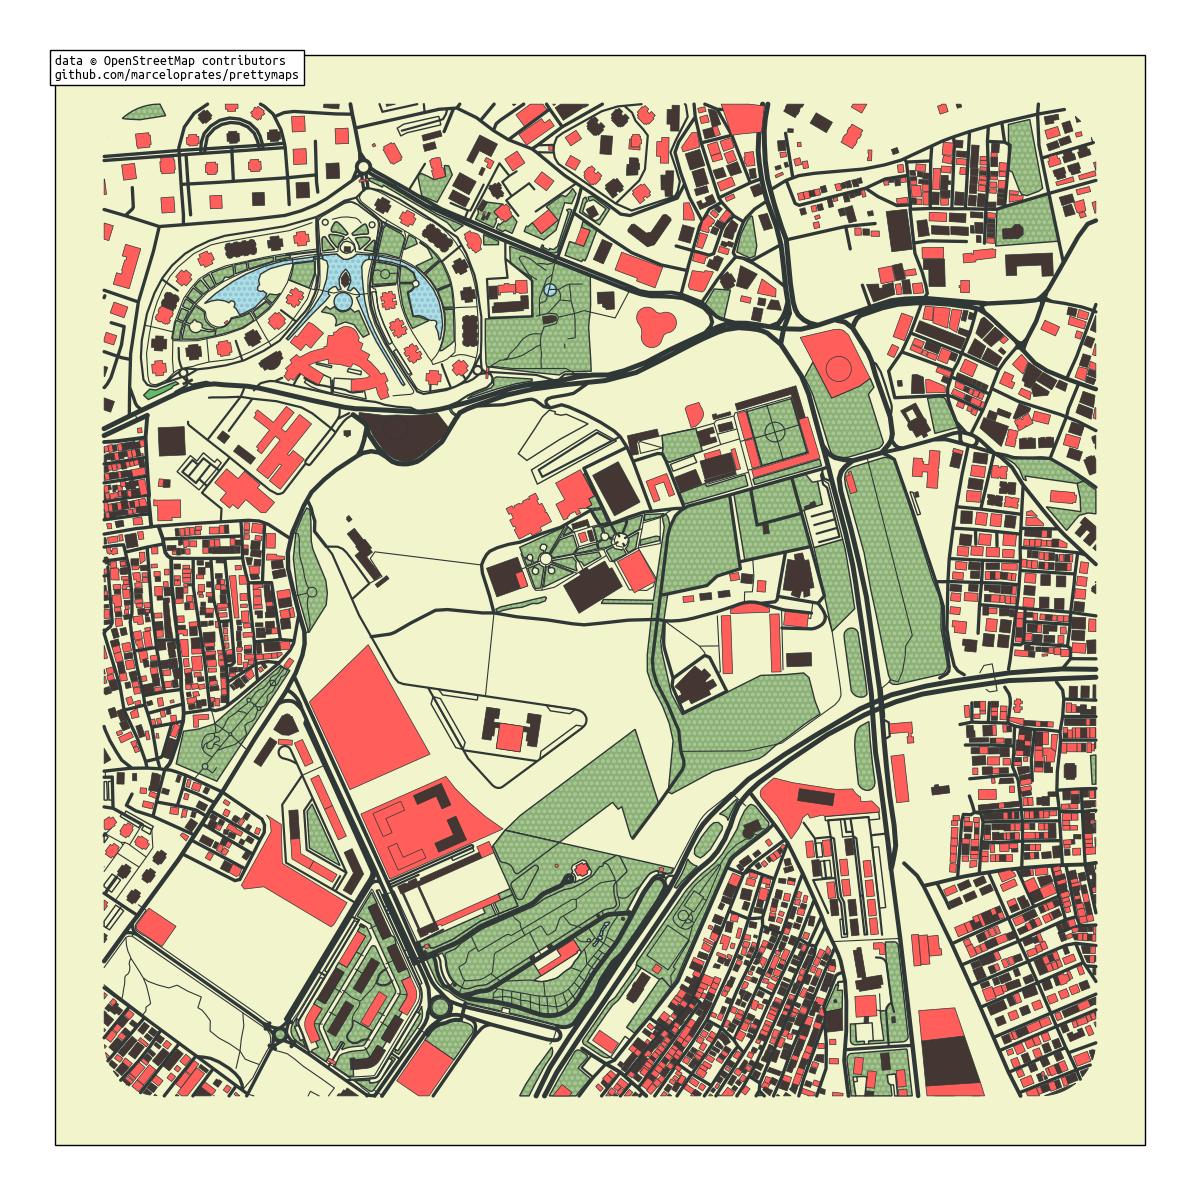
\includegraphics[width=0.5\textwidth]{images/izu.png}
    \caption{Prettymaps IZU.}
    \label{fig:enter-label}
\end{figure}

\newpage

\subsection{Scikeras - Keras HP Tuning}
\begin{lstlisting}[language=Python]
import tensorflow as tf
from scikeras.wrappers import KerasClassifier
from sklearn.model_selection import GridSearchCV

def create_model(units=16, lr_rate=0.1):
    model = tf.keras.Sequential()
    model.add(tf.keras.layers.Dense(units, activation='relu'))
    model.add(tf.keras.layers.Dense(num_classes, activation='softmax'))
    model.compile(optimizer=tf.keras.optimizers.Adam(learning_rate=lr_rate),
                  loss='categorical_crossentropy',
                  metrics=['accuracy'])
    return model

units = [16, 32]
lr_rate = [0.1,0.001]
batch_size = [128, 64]

keras_model = KerasClassifier(build_fn=create_model, 
                              units=units, 
                              lr_rate=lr_rate, 
                              epochs=10, 
                              batch_size=batch_size, 
                              callbacks=[EarlyStopping(monitor='val_loss', patience=3)], 
                              verbose=0)

param_grid = dict(units = units, lr_rate = lr_rate, batch_size = batch_size)
grid = GridSearchCV(estimator = keras_model, param_grid = param_grid, cv = 3)
grid_result = grid.fit(train_data, train_labels)
print("The best parameters are:",grid_result.best_params_)
best_params = grid_result.best_params_
\end{lstlisting}

\subsection{pyLDAvis - Topic Modeling with LDA}
\begin{lstlisting}[language=Python]
import gensim
import pyLDAvis.gensim

tokenized = df["Lemmatization"]
tokenized = [token.split(" ") for token in tokenized]
dictionary = corpora.Dictionary(tokenized)
dictionary.filter_extremes(no_below=1, no_above=0.8)
corpus = [dictionary.doc2bow(tokens) for tokens in tokenized]

ldamodel = gensim.models.ldamodel.LdaModel(corpus, num_topics = 8, id2word=dictionary, passes=15)
lda_display = pyLDAvis.gensim.prepare(ldamodel, corpus, dictionary, sort_topics=True)
pyLDAvis.display(lda_display)
\end{lstlisting}

\subsection{visualkeras - 3D Model Visualization}
\begin{lstlisting}[language=Python]
import tensorflow as tf
import visualkeras

model = tf.keras.Sequential()
model.add(tf.keras.layers.Conv2D(32, (3, 3), activation='relu', input_shape=(224, 224, 3)))
model.add(tf.keras.layers.MaxPooling2D((2, 2)))
model.add(tf.keras.layers.Conv2D(64, (3, 3), activation='relu'))
model.add(tf.keras.layers.MaxPooling2D((2, 2)))
model.add(tf.keras.layers.Conv2D(64, (3, 3), activation='relu'))
model.add(tf.keras.layers.Flatten())
model.add(tf.keras.layers.Dense(32, activation='relu'))
model.add(tf.keras.layers.Dense(10, activation='softmax'))
model.compile(optimizer=tf.keras.optimizers.Adam(),
              loss='categorical_crossentropy',
              metrics=['accuracy'])

visualkeras.layered_view(model, to_file="visualkeras.png").show()
\end{lstlisting}

\begin{figure}[ht]
    \centering
    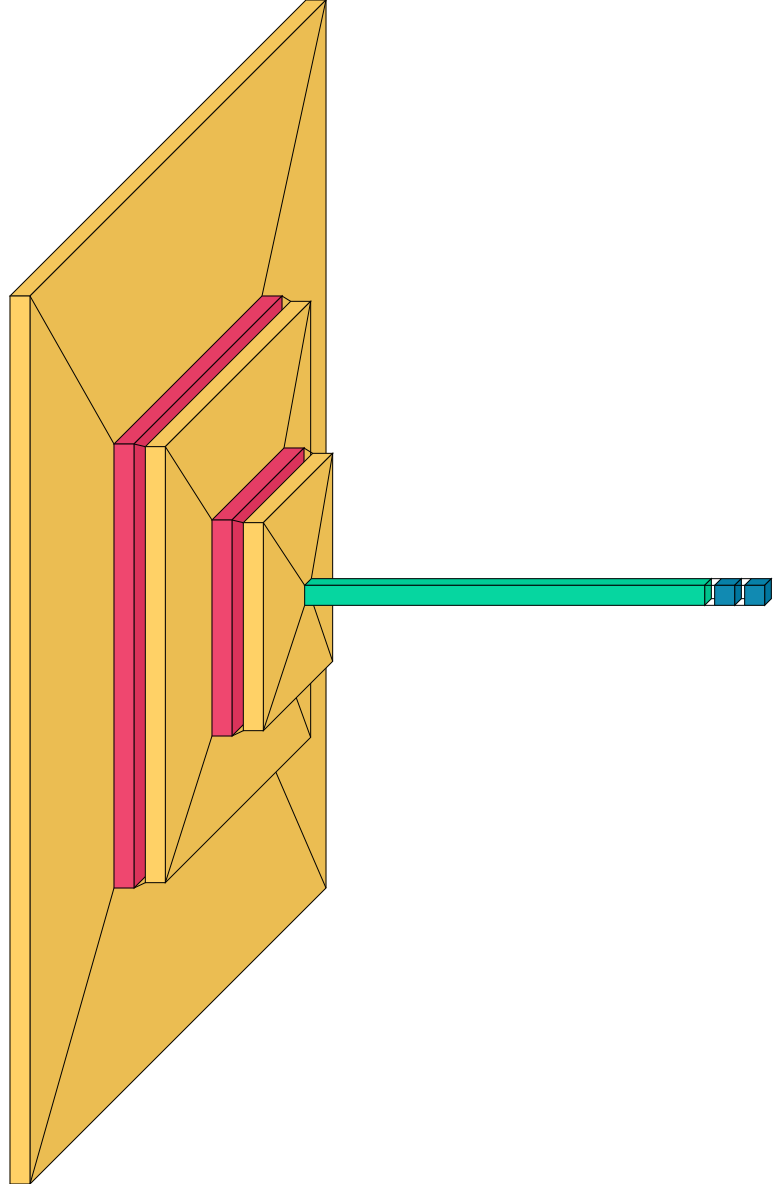
\includegraphics[width=0.25\textwidth]{images/visualkeras.png}
    \caption{visualkeras .}
    \label{fig:enter-label}
\end{figure}

\newpage

\subsection{Plotting N-Grams}
\begin{lstlisting}[language=Python]
def count_ngrams(corpus, ngram, n):
    vec = CountVectorizer(ngram_range=(ngram,ngram)).fit(corpus)
    bag_of_words = vec.transform(corpus)
    sum_words = bag_of_words.sum(axis=0)
    words_freq = [(word, sum_words[0, idx]) for word, idx in vec.vocabulary_.items()]
    words_freq =sorted(words_freq, key = lambda x: x[1], reverse=True)
    return words_freq[:n]
    
def plot_ngrams(ngram_df, ngram_name):
    plt.figure(figsize=(12, 6))
    plt.bar(data=ngram_df, x="Tweets", height="Count")
    plt.xticks(rotation=90)
    plt.xlabel(ngram_name)
    plt.ylabel("Count")
    plt.title(ngram_name)
    plt.show()
    
unigrams = count_ngrams(corpus=df["Lemmatization"], ngram=1, n=30)
top_unigram = pd.DataFrame(unigrams, columns=['Tweets', "Count"])
plot_ngrams(top_unigram, "Unigrams")
\end{lstlisting}

\begin{figure}[ht]
    \centering
    \includegraphics[width=1.0\textwidth]{images/nlp_unigram.png}
    \caption{Unigrams .}
    \label{fig:enter-label}
\end{figure}

\newpage


\section{---------------- MAKİNE ÖĞRENMESİ KISMI ----------------}
\newpage
\section{Analiz Yöntemleri}
\subsection{Cohort Analizi}
Cohort analizi, bir işletmenin müşteri davranışlarını ve performansını daha iyi anlamak için kullanılan bir veri analizi yöntemidir. Bu yöntem, benzer özelliklere sahip müşteri gruplarını (cohort) oluşturarak, bu grupların zaman içindeki davranışlarını izlemeyi sağlar. Cohort analizinin temel amacı, belirli bir dönemde birlikte başlayan ve benzer özelliklere sahip müşteri gruplarını tanımlamak ve bu grupların performansını izlemek için kullanılır. Cohort analizi, özellikle müşteri sadakati, terk oranları ve gelir analizi gibi konularda işletmelere değerli bilgiler sunar.

\begin{lstlisting}[language=Python, caption=Cohort analizi örneği]
import pandas as pd

# Ornek bir veri cercevesi olusturalim
data = {'Tarih': ['2023-01-01', '2023-01-01', '2023-02-01', '2023-02-01'],
        'MusteriID': [1, 2, 3, 4],
        'Gelir': [100, 150, 200, 50]}

df = pd.DataFrame(data)

# Musteri kaydi tarihine gore cohort olusturma
df['Cohort'] = df.groupby('Tarih')['MusteriID'].transform('min')

# Cohort analizi icin gruplama
cohorts = df.groupby(['Cohort', 'Tarih'])['Gelir'].sum().unstack()

# Her cohort'in ilk aydaki performansini hesaplama
cohort_size = cohorts.iloc[:, 0]
cohorts = cohorts.divide(cohort_size, axis=0)

# Sonuclari yazdirma
print(cohorts)
\end{lstlisting}

\subsection{RFM Analizi}
RFM analizi, bir işletmenin müşterilerini segmentlere ayırmak ve müşteri davranışını daha iyi anlamak amacıyla kullanılan bir pazarlama analizi yöntemidir.

\begin{itemize}
    \item \textbf{Recency (Yenilik):} Müşterinin son aktivitesinin (örneğin, son satın alma) ne kadar yakın zamanda gerçekleştiğini belirtir. Genellikle bu süre içindeki geçmiş tarih ile analiz yapılır.
    \item \textbf{Frequency (Sıklık):} Müşterinin belirli bir zaman diliminde (örneğin, son bir yıl) yaptığı toplam işlem veya etkileşim sayısını belirtir. Bu sıklık, müşterinin işletmeye ne kadar sık geri döndüğünü yansıtır.
    \item \textbf{Monetary (Parasal Değeri):} Müşterinin toplam gelir veya harcama miktarını belirtir. Bu, müşterinin işletmeye ne kadar para harcadığıını yansıtır.
\end{itemize}

\begin{lstlisting}[language=Python, caption=RFM analizi örneği]
import pandas as pd

# Ornek bir veri cercevesi olusturalim
data = {'MusteriID': [1, 2, 3, 4, 5],
        'Tarih': ['2023-09-10', '2023-10-15', '2023-08-20', '2023-07-05', '2023-09-25'],
        'Miktar': [100, 150, 200, 50, 300]}

df = pd.DataFrame(data)
df['Tarih'] = pd.to_datetime(df['Tarih'])

# Recency hesaplama
max_date = df['Tarih'].max()
df['Recency'] = (max_date - df['Tarih']).dt.days

# Frequency hesaplama
frequency = df.groupby('MusteriID')['Tarih'].count().reset_index()
frequency.rename(columns={'Tarih': 'Frequency'}, inplace=True)
df = df.merge(frequency, on='MusteriID', how='left')

# Monetary hesaplama
monetary = df.groupby('MusteriID')['Miktar'].sum().reset_index()
monetary.rename(columns={'Miktar': 'Monetary'}, inplace=True)
df = df.merge(monetary, on='MusteriID', how='left')

# RFM puanlarini hesaplama
# Isletmenizin kendi puanlama ve segmentasyon kriterlerini tanimlamalisiniz.

# Ornek: Recency icin, daha dusuk degerler daha iyi oldugunu varsayalim.
df['RecencyScore'] = pd.qcut(df['Recency'], q=5, labels=False)

# Ornek: Frequency ve Monetary icin, daha yuksek degerler daha iyi oldugunu varsayalim.
df['FrequencyScore'] = pd.qcut(df['Frequency'], q=5, labels=False)
df['MonetaryScore'] = pd.qcut(df['Monetary'], q=5, labels=False)

# RFM toplam puanini hesaplama
df['RFMScore'] = df['RecencyScore'] + df['FrequencyScore'] + df['MonetaryScore']

# Sonuclari goruntuleme
print(df)
\end{lstlisting}

\subsection{CRM Analizi}
CRM Analizi (Customer Relationship Management Analysis), müşteri ilişkileri yönetimi süreçlerini incelemek, geliştirmek ve optimize etmek için kullanılan bir veri analizi yöntemidir. CRM Analizi, müşteri ilişkilerini daha iyi anlamak, müşteri memnuniyetini artırmak, satışları artırmak ve işletme karlılığını geliştirmek amacıyla kullanılır.

\begin{lstlisting}
import pandas as pd

# Ornek bir musteri veri cercevesi olusturalim
data = {'Musteri_ID': [1, 2, 3, 4, 5],
        'Musteri_Adi': ['Alice', 'Bob', 'Charlie', 'David', 'Eve'],
        'Satin_Alma_Miktari': [100, 150, 200, 50, 300],
        'Sikayet_Sayisi': [2, 0, 1, 3, 0],
        'Ziyaret_Sikligi': [5, 3, 8, 2, 10]}

df = pd.DataFrame(data)

# Ornek bir CRM analizi yapalim
# Isletmenize ozgu analiz kriterlerinizi ve hedeflerinizi burada belirlemeniz gerekmektedir.

# Ornek: Musteri sadakatini degerlendirmek icin "Satin_Alma_Miktari" ve "Ziyaret_Sikligi" degerlerini kullanalim
df['Sadakat_Skoru'] = (df['Satin_Alma_Miktari'] * 0.6) + (df['Ziyaret_Sikligi'] * 0.4)

# Ornek: Sikayet sayisini inceleyerek hizmet kalitesini degerlendirelim
df['Hizmet_Kalitesi'] = df['Sikayet_Sayisi'].apply(lambda x: 'Kotu' if x > 2 else 'Iyi')

# Sonuclari goruntuleme
print(df)
\end{lstlisting}

\subsection{CLV Analizi}
CLV (Customer Lifetime Value), bir işletmenin müşterilerinin yaşam boyu gelirini tahmin etmek için kullanılan önemli bir metriktir. CLV, bir müşterinin işletmeyle ilişkisi boyunca yarattığı geliri hesaplayarak, işletmelere, müşterilerini daha iyi anlama, pazarlama stratejilerini optimize etme ve müşteri sadakatini artırma konularında yardımcı olur. CLV Formülü:

\[\text{CLV} = \frac{\text{Musterinin Ortalama Satin Alma Degeri * Satin Alma Sikliği * Musterinin Omru}}{\text{İndirim Orani}}\]

Bu formülde:
\begin{itemize}
    \item \textbf{Müşterinin Ortalama Satın Alma Değeri:} Bir müşterinin ortalama bir satın alma işlemi sırasında harcadığı miktar.
    \item \textbf{Satın Alma Sıklığı:} Bir müşterinin belirli bir zaman diliminde (örneğin, bir yıl) ne sıklıkta satın alma işlemi yaptığı.
    \item \textbf{Müşterinin Ömrü:} Bir müşterinin işletme ile ilişkisi boyunca geçirdiği süre (aylar veya yıllar cinsinden).
    \item \textbf{İndirim Oranı:} İşletme tarafından verilen indirimler veya kampanyaların etkisiyle düzeltilen bir faktör. Bazı müşteriler daha fazla indirim alabilir.
\end{itemize}

\begin{lstlisting}[language=Python, caption=CLV analizi örneği.]
import pandas as pd

# Ornek bir musteri veri cercevesi olusturalim
data = {'Musteri_ID': [1, 2, 3, 4, 5],
        'Musteri_Adi': ['Alice', 'Bob', 'Charlie', 'David', 'Eve'],
        'Toplam_Harcama': [1000, 1500, 2000, 500, 3000],
        'Satin_Alma_Sikligi': [5, 3, 8, 2, 10],
        'Musteri_Omru': [24, 36, 60, 12, 48]}

df = pd.DataFrame(data)

# Ortalama satin alma degeri hesaplama
df['Ortalama_Satin_Alma_Degeri'] = df['Toplam_Harcama'] / df['Satin_Alma_Sikligi']

# CLV hesaplama
indirim_orani = 0.1  # Ornek bir indirim orani
df['CLV'] = (df['Ortalama_Satin_Alma_Degeri'] * df['Satin_Alma_Sikligi'] * df['Musteri_Omru']) / (1 + indirim_orani)

# Sonuclari goruntuleme
print(df)
\end{lstlisting}

\newpage
\section{ARD Regression}
ARDRegression (Automatic Relevance Determination Regression), L1 ve L2 regularizasyon yöntemlerini birleştirerek çalışır.

\subsection{Hiperparametreler}

\begin{table}[h]
\centering
{\scriptsize\renewcommand{\arraystretch}{0.1}
{\resizebox*{\linewidth}{0.8\textwidth}{
\begin{tabular}{|p{2cm}|p{1cm}|p{1cm}|p{6cm}|}
\hline
Parametre & Type & Default & Açıklama  \\ \hline
tol & float & 1e-3 & w yakınsadıysa algoritmayı durdurur.  \\ \hline
alpha\_1 & float & 1e-6 & L1 düzenlemesi katsayısıdır. Bu parametre arttıkça L1 düzenlemesi etkisi artar.  \\ \hline
alpha\_2 & float & 1e-6 & L2 düzenlemesi katsayısıdır. Bu parametre arttıkça L2 düzenlemesi etkisi artar.  \\ \hline
lambda\_2 & float & 1e-6    & Intercept (kesme noktası) için L2 düzenlemesi katsayısıdır. \\ \hline
compute\_score & bool & False & True ise modelin her adımında amaç fonksiyonunu hesaplar.  \\ \hline
threshold\_lamda & float & 10000 & Yüksek hassasiyete sahip ağırlıkların hesaplamadan çıkarılması (budanması) için eşik.  \\ \hline
fit\_intercept & bool  & True & Kesişimin (intercept) uydurulup uydurulmayacağı.  \\ \hline
copy\_X & bool & True & Eğer True ise modeli eğitirken X değeri fonksiyonda kullanılacak ve eğitimden sonra da aynı olacaktır. False olduğunda ise X fonksiyona girdikten sonra ilk hali ile aynı olmayabilir. \\ \hline
verbose & bool  & False   & True ise çıktı gösterir.  \\ \hline
\end{tabular}
}}}
\end{table}

\newpage
\section{Adaptive Boosting}
Zayıf öğrenicileri bir araya getirerek güçlü bir öğrenici oluşturmak için kullanılan bir toplu öğrenme yöntemidir.

\subsection{Çalışma Adımları}
\begin{enumerate}
    \item Her bit örnek başlangıçta 1/N ağırlığına sahiptir. N, toplam örnek sayısı.
    \item Bir zayıf öğrenici eğitilir.
    \item Zayıf öğrenicinin doğruluğu hesaplanır.
    \item Doğruluğu düşük olan örneklerin ağırlığı arttırılır. Bu, yanlış sınıflandırılan örneklerin daha fazla dikkate alınmasını sağlar. Modelin bu örnekleri daha iyi sınıflandırması beklenir.
    \item Ağırlıklandırılmış eğitim veri seti, bir sonraki zayıf öğreniciyi eğitmek için kullanılır. Bu süreç, belli bir iterasyon (boosting round) için tekrarlanır.
    \item Her bir zayıf öğrenici, tahminlerin gücüne göre bir ağırlıkla birleştirilir. Bu ağırlıklandırma işlemi, her bir öğreticinin doğruluğuna göre belirlenir. Daha doğru tahminler, daha büyük ağırlığa sahip olur.
    \item Zayıf öğrenicilerin bir araya getirilmesiyle güçlü bir öğrenici elde edilir.
\end{enumerate}

\subsection{Hiperparametreler}

\begin{table}[h]
\centering
{\scriptsize\renewcommand{\arraystretch}{0.4}
{\resizebox*{\linewidth}{0.3\textwidth}{
\begin{tabular}{|p{2cm}|p{1cm}|p{1cm}|p{6cm}|}
\hline
Parametre & Type & Default & Açıklama \\ \hline
estimator & object & None & Kullanılacak zayıf öğrenici türü. \\ \hline
n\_estimators & float & 1e-6 & Kullanılacak zayıf öğrenici sayısı. Fazla olması karmaşıklığı ve overfit'i artırabilir.  \\ \hline
learning\_rate & float & 1e-6 & Her bir zayıf öğrenicinin katkısını artırmak veya azaltmak için kullanılan parametre.  \\ \hline
loss & float & 1e-6 & Kayıp fonksiyonu.  \\ \hline
random\_state & bool & False & Rastgelelik kontrolü. \\ \hline
\end{tabular}
}}}
\end{table}

\newpage
\section{Bayesian Ridge}
Bayes teoremini ve bayes istatistik prensiplerine dayanarak lineer regresyon temelli bir modeldir. Bayes teoremi kullanarak olasılık dağılmını güncelleyerek parametreleri belirler.

\subsection{Çalışma Adımları}
\begin{enumerate}
    \item Bir önceki dağılım (prior distribution) belirlenir. Bu, parametrelerin olası değerleri hakkında bir öngörü sağlar.
    \item Problemi bir olasılık dağılımı olarak ele alır.
    \item Veri dağılımına bağlı olarak bir olasılık fonksiyonu (likelihood function) belirlenir. Bu fonksiyon, modelin parametrelerinin belirli bir değere sahip olma olasılığını tanımlar.
    \item Model, veriye dayalı olarak bayes teoremini kullanarak önceki dağılımları günceller.
    \item Güncellenmiş dağılımlar modelin parametreleri için bir sonraki dağılımı (posterior distribution) oluşturur.
    \item Model bu dağılımı kullanarak tahmin yapar.
\end{enumerate}

\begin{table}[ht]
\centering
{\scriptsize\renewcommand{\arraystretch}{0.4}
{\resizebox*{\linewidth}{0.4\textwidth}{
\begin{tabular}{|p{2cm}|p{1cm}|p{1cm}|p{6cm}|}
\hline
Parametre & Type & Default & Açıklama \\ \hline
alpha\_1 & float & 1e-6 & Prior distribution için L2 regularizasyon hassasiyeti.  \\ \hline
alpha\_2 & float & 1e-6 & Likelihood function için L2 regularizasyon hassasiyeti.  \\ \hline
lambda\_1 & float & 1e-6 & Prior distribution için L1 regularizasyon hassasiyeti.  \\ \hline
lambda\_2 & float & 1e-6 & Likelihood function için L1 regularizasyon hassasiyeti. \\ \hline
tol & float & 1e-3 & Optimizasyon algoritmasının toleransı. \\ \hline
\end{tabular}
}}}
\end{table}

\newpage
\section{Kalibrasyon Metodları}
Kalibrasyon, modelin çıktılarını gerçek olasılıklara daha yakın hale getirmeyi amaçlar.
\begin{enumerate}
    \item Platt Scaling (Sigmoid Fitting)
    \item Isotonic Regression
    \item Beta Calibration
    \item Platt's Method Extension
    \item Venn-ABERS Method
\end{enumerate}

\begin{figure}[h]
    \centering
    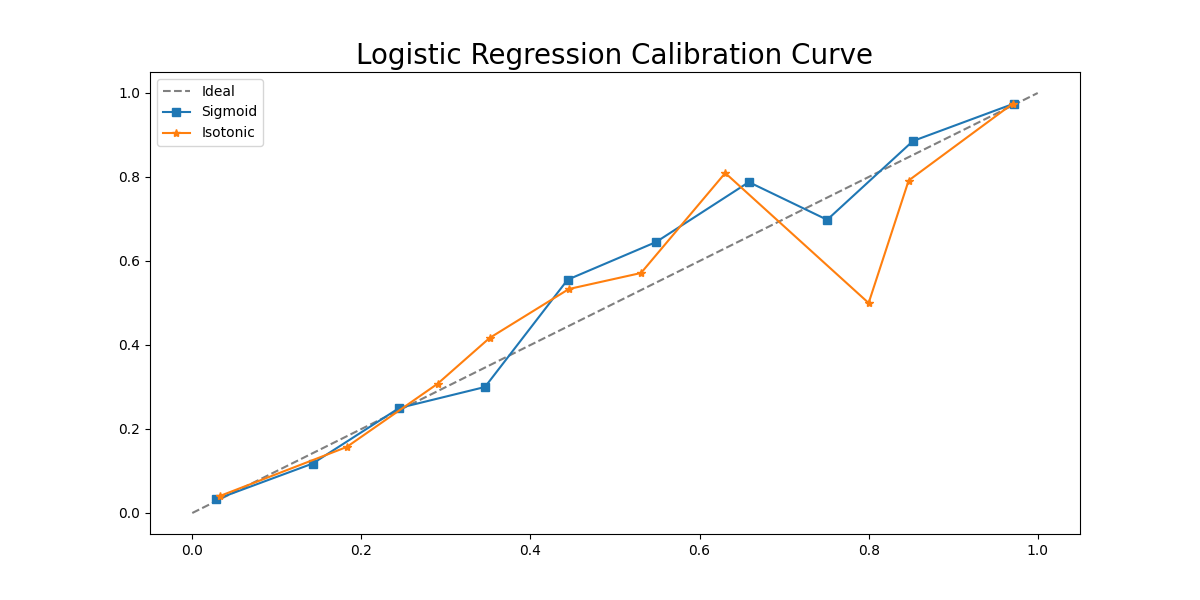
\includegraphics[width=1\textwidth]{images/calibration.png}
    \caption{Isotonic-Sigmoid kalibrasyon metodları.}
    \label{fig:enter-label}
\end{figure}

\subsection{Platt Scaling (Sigmoid Fitting)}
Adını John Platt'ten alır. Genellikle sigmoid fonksiyonu ile gerçekleştirilir. İlk olarak sınıflandırıcı çıktıları log-odds'a dönüştürülür. Ardından, log-odds değerleri sigmoid fonksiyonuna geçirilir. Bu olasılıkları [0, 1] aralığına yeniden ölçekler. Temel fikir modelin tahmin edilen sınıf olasılıklarına bir lojistik regresyon modeli uydurmaktır. Lojistik regresyon modeli, tahmin edilen olasılıklara dayalı olarak gerçek sınıf etiketlerini tahmin etmek üzere eğitilir ve modelin katsayıları tahmin edilen olasılıkları kalibre edilmiş olasılıklara dönüştürmek için kullanılır.

\[\text{platt\_cal} = \frac{1}{(1 + \exp(-z))}\]
\[\text{z} = \log(\frac{p}{1 - p})\]

\begin{lstlisting}[language=Python, caption=Scikit-learn'de Platt scaling örneği.]
from sklearn.calibration import CalibratedClassifierCV

svm = SVC(probability=True, random_state=42)
svm.fit(X_train, y_train)

calibrated_svm = CalibratedClassifierCV(svm, method='sigmoid', cv='prefit')
calibrated_svm.fit(X_train, y_train)

probabilities_before = svm.predict_proba(X_test)[:, 1]
probabilities_after = calibrated_svm.predict_proba(X_test)[:, 1]
\end{lstlisting}

\subsection{Isotonic Regression}
Olasılık tahminlerini düzgünleştirmek için monoton artan bir fonksiyonla uyumlu hale getirir. İlk olarak, modelin olasılık tahminleri sıralanır. Monoton artan bir fonksiyon olan isotonic regression kullanılır. Bu regresyon, sıralı tahminler arasında bir düzgünleştirme yaparak olasılık tahminlerini yeniden ölçekler. İzotonik, olasılıkların sırasını korur.

\begin{lstlisting}[language=Python, caption=Scikit-learn'de Isotonic Regression örneği.]
from sklearn.calibration import CalibratedClassifierCV
from sklearn.isotonic import IsotonicRegression

svm = SVC(probability=True, random_state=42)
svm.fit(X_train, y_train)

calibrated_svm = CalibratedClassifierCV(svm, method='sigmoid', cv='prefit')
calibrated_svm.fit(X_train, y_train)

probabilities_after = calibrated_svm.predict_proba(X_test)[:, 1]

isotonic_regressor = IsotonicRegression(out_of_bounds='clip')
isotonic_regressor.fit(probabilities_after, y_test)

probabilities_isotonic = isotonic_regressor.transform(probabilities_after)
\end{lstlisting}

\subsection{Beta Calibration}
Olasılık tahminlerini uygun bir şekilde düzgünleştirmek için beta dağılımını kullanır. İlk olarak, modelin olasılık tahminleri log-odds'a dönüştürülür. Ardından log-odds değerleri beta dağılımına uydurulur. Beta dağılımı [0, 1] aralığındaki değerleri modellere uygulayarak olasılık tahminlerini yeniden ölçekler.

\begin{lstlisting}[language=Python, caption=Scikit-learn'de Beta Calibration örneği.]
from sklearn.calibration import CalibratedClassifierCV
from sklearn.calibration import calibration_curve

svm = SVC(probability=True, random_state=42)
svm.fit(X_train, y_train)

calibrated_svm = CalibratedClassifierCV(svm, method='sigmoid', cv='prefit')
calibrated_svm.fit(X_train, y_train)

probabilities_after = calibrated_svm.predict_proba(X_test)[:, 1]

def beta_calibration(probabilities):
    sorted_probs = np.sort(probabilities)
    beta_values = np.linspace(0.5, len(sorted_probs) - 0.5, len(sorted_probs)) / len(sorted_probs)
    calibrated_probs = np.clip(np.interp(probabilities, sorted_probs, beta_values), 0, 1)
    return calibrated_probs

probabilities_beta = beta_calibration(probabilities_after)
\end{lstlisting}

\subsection{Platt's Method Extension}
Sigmoid dönüşümü yerine, daha genel bir logit dönüşümünü kullanır. İlk olarak modelin olasılık tahminleri logit dönüşümüne tabi tutulur. Elde edilen değerler üzerinde doğrusal bir regresyon modeli kurulur. Bu model, olasılık tahminlerini ölçeklemek için kullanılır.

\begin{lstlisting}[language=Python, caption=Scikit-learn'de Platt's Method örneği.]
from sklearn.calibration import CalibratedClassifierCV

svm = SVC(probability=True, random_state=42)
svm.fit(X_train, y_train)

calibrated_svm = CalibratedClassifierCV(svm, method='sigmoid', cv='prefit')
calibrated_svm.fit(X_train, y_train)

logit_transformed_probs = calibrated_svm.predict_proba(X_test)[:, 1] 

lr = LogisticRegression()
lr.fit(logit_transformed_probs.reshape(-1, 1), y_test)

scaled_probs = lr.predict_proba(logit_transformed_probs.reshape(-1, 1))[:, 1]
\end{lstlisting}

\subsection{Venn-ABERS}
Modelin tahminleri, modelin tahmin ettiği sınıfların gerçekte hangi oranda gerçekleştiğini gösteren bir referans dağılım ile karşılaştırılır. Karşılaştırma sonucunda, modelin tahminlerinin gerçek tahminlerden ne kadar saptığı hesaplanır. Bu sapmalar modelin tahminlerini düzeltmek için kullanılır. Dengesiz veri setlerinde etkilidir.

\begin{lstlisting}[language=Python, caption=venn\_abers kütüphanesi ile örnek.]
from venn_abers import VennAbersCalibrator
from xgboost import XGBClassifier
xgb = XGBClassifier().fit(X_train, y_train)
p_test = xgb.predict_proba(X_test)
p_cal = xgb.predict_proba(X_calib)
vac = VennAbersCalibrator()
# Inductive
ivap = vac.predict_proba(p_cal=p_cal, y_cal=y_calib, p_test=p_test)[:, 1]
# Cross
vac_c = VennAbersCalibrator(estimator=xgb, inductive=False, n_splits=10).fit(X_train, y_train)
cvap = vac_c.predict_proba(X_test)[:, 1]
\end{lstlisting}

\subsection{Metrikler}
\begin{itemize}
    \item \textbf{Brier Score:} Gerçek sınıf etiketleri ile tahmin edilen olasılıklar arasındaki farkların karesinin ortalamasıdır. Düşük brier skoru, daha iyi kalibre edilmiş bir modeli gösterir.
    \begin{equation*}
    \text{Brier Skoru} = \frac{1}{N} \sum_{i=1}^{N} (f_i - o_i)^2
    \end{equation*}
    
    Burada:
    \begin{itemize}
        \item $f_i$, $i$'inci örneğin tahmin edilen olasılığı,
        \item $o_i$, $i$'inci örneğin gerçek olasılığıdır.
    \end{itemize}
    \item \textbf{Reliability Diagram:} Gerçek sınıf olasılıkları ve modelin tahmin ettiği olasılıklar arasındaki ilişkiyi gösterir.
    \item \textbf{Calibration Curve:} Gerçek ve tahmin edilen olasılıklar arasındaki ilişkiyi görselleştiren bir eğridir. İdeal olarak eğri doğrusal olmalıdır.
\end{itemize}

\newpage
\section{CatBoost}
Yandex tarafından geliştirilmiştir. 2017 yılında Prokhorenkova ve diğerleri tarafından 'CatBoost: unbiased boosting with categorical features' isimli makalede tanılmıştır. Adını 'Category' ve 'Boosting' kelimelerinin birleşiminden alır. CatBoost, ağaç tabanlı bir modeldir ve gradient boosting yöntemini kullanır. Kategorik değerleri otomatik olarak kodlayabilir, boş değerler ve aykırı değerler ile başa çıkarak ön işleme adımını hızlandırır. GPU desteği bulunur. CatBoost, simetrik ağaçlar kurarak çok derin ağaçlar oluşturmadan başarılı sonuçlar elde eder ve aşırı öğrenme sorununun üstesinden gelir.

\subsection{Çalışma Adımları}
\begin{enumerate}
	\item İlk olarak başlangıç tahminleri (initial prediction) yapılır. İlk tahminler, hedef değişkenin ortalaması veya bir sabit değerle yapılır.  Bu, daha sonra modelin hatalarını azaltmak için kullanılır.
	\item Ardışık ağaçlar oluşturarak boosting süreci uygulanır. Her ağaç, hedef değişkenin tahminini iyileştirmek için oluşturulur.
	\item Her ağacı oluştururken rastgele özellik seçimi yaparak her ağacın farklı bir alt kümeyi kullanmasını sağlar.
	\item Ağaçlar oluşturulduktan sonra, hata fonksiyonunu minimize etmek için optimize edilir.
	\item Her iterasyonda mevcut modelin hatalarını azaltacak yeni bir ağaç ekler.
\end{enumerate}

\subsection{Hiperparametreler}
\begin{table}[h]
\centering
{\scriptsize\renewcommand{\arraystretch}{0.4}
{\resizebox*{\linewidth}{0.4\textwidth}{
\begin{tabular}{|p{3cm}|p{1cm}|p{1cm}|p{6cm}|}
\hline
Parametre & Type & Default & Açıklama \\ \hline
learning\_rate & float & 1e-3 & Öğrenme oranı. \\ \hline
iterations & float & 1e-6 & Boosting aşamasındaki ağaç sayısı. \\ \hline
depth & float & 1e-6 & Her bir ağacın derinliği. \\ \hline
l2\_leaf\_reg & float & 1e-6 & L2 düzenleme. \\ \hline
bagging\_temperature & bool & False & Seed. Boosting örneklemesi sırasında kullanılır. \\ \hline
border\_count & float & 10000 & Sayısal özelliklerin kuantize edilmesi. \\ \hline
random\_strength & bool & True & Rastgele örneklemleme sırasında özelliklerin güçlendirilmesi için kullanılan güçlendirme katsayısı. \\ \hline
leaf\_estimation\_method & bool & True & Ağaç yapraklarının tahmin yöntemi. \\ \hline
grow\_policy & bool & False & Ağaç büyüme stratejisi. \\ \hline
\end{tabular}
}}}
\end{table}

\newpage
\section{Causal Interpretation}
Modelin verilerden neden-sonuç ifadelerini çıkarabilmesidir. Nedensel ilişkilerin anlaşılması, sadece belirli bir olayın diğerini takip ettiği zamansal sıra veya ilişkisel korelasyonlardan daha fazlasını içerir. Bu, bir değişkenin başka bir değişkeni doğrudan etkileyebileceği ve bu etkinin nedensel olduğu anlamına gelir.

\newpage

\subsection{CATE (Conditional Average Treatment Effect)}
CATE, belirli bir müdahalenin veri üzerinde ortalama olarak ne tür bir etkiye sahip olduğunu gösterir. Bu etki diğer özelliklere bağlı olarak değişebilir. Nedensel etkileri incelemek için kullanılır. Teknikler:

\begin{enumerate}
    \item Double Machine Learning
    \item Doubly Robust
    \item Meta-Learner
    \item Orthogonal Random Forest
\end{enumerate}

\newpage

\subsection{Double Machine Learning}
Çift model yaklaşımını kullanır. İki farklı model ile tahminler yapar ve bu tahminler arasındaki farkı analiz eder. İki model genellikle bir denklem ve bir tahminci model olarak adlandırılır.

\begin{enumerate}
    \item \textbf{Denklem modeli:} Bağımsız değişkenler ve sonucun tahmin edilmesi için kullanılır.
    \item \textbf{Tahminci model:} Bağımsız değişkenlerin sonucunu tahmin etmek için kullanılır. Denklem modelininin yanıltıcı bir şekilde etkilenmemesi sağlanmalıdır.
\end{enumerate}

\subsubsection{Python Kodu}

\begin{lstlisting}[language=Python, caption=ecoml'de DML örneği.]
from econml.dml import DML
from econml.sklearn_extensions.linear_model import StatsModelsLinearRegression
from sklearn.ensemble import RandomForestRegressor, RandomForestClassifier

est = DML(
	model_y=RandomForestRegressor(),
	model_t=RandomForestClassifier(),
	model_final=StatsModelLinearRegression()
)
est.fit(y, T, X=X, W=None)
\end{lstlisting}

\newpage

\subsection{Double Robust}
Çift model yaklaşımını kullanır. Kısmi modelden gelen tahminler kullanılarak doğrudan bir tahmin yapılır. Tahmin modelinden gelen tahminler kullanılarak müdahalenin etkisi tahmin edilir. Bu iki tahmin arasındaki fark, müdahalenin gerçek etkisini belirlemek için kullanılır.

\begin{enumerate}
    \item \textbf{Partial Model:} Kovaryanslar ve diğer değişkenler ile bağımlı değişken arasındaki ilişkiyi belirler.
    \item \textbf{Tahmin Modeli:} Müdahalenin etkisini tahmin etmek için kullanılır.
\end{enumerate}

\subsubsection{Python Kodu}

\begin{lstlisting}[language=Python, caption=econml'de Double Robust örneği.]
from eeconml.dr import LinearDRLearner

est = LinearDRLearner()
est.fit(y, T, X=X, W=None)
\end{lstlisting}

\newpage

\subsection{Meta-Learners}
Birincil bir modelin çıktısını kullanarak ikincil bir modeli eğiten modeldir. Bu sayede birincil modelin performansını iyileştirir ve onun çıktılarını daha iyi bir şekilde kullanır.

\subsubsection{Python Kodu}

\begin{lstlisting}[language=Python, caption=econml'de Meta-Learner örneği.]
from econml.metalearners import XLearner
from sklearn.linear_model import LinearRegression

est = XLearner(models=LinearRegression())
est.fit(y, T, X=X)
\end{lstlisting}

\newpage

\subsection{Orthogonal Random Forest}
ORF, RF algoritmasına çıkarımlar için uygun hale getirmek bir düzeltme yapar. Bu düzeltme, karar ağaçlarının gözlemlenen veriler üzerinden değil, önceki çalışmalardan elde edilen tahminler üzerinde eğitilmesini sağlar. Bu tahminler, müdahalenin etkisini doğrudan tahmin etmek için kullanılır.

\newpage
\section{Kümeleme Metodları} 
\begin{enumerate}
    \item AffinityPropagation
    \item AgglomerativeClustering
    \item Birch
    \item DBSCAN
    \item FeatureAgglomeration
    \item KMeans
    \item MeanShift
    \item MiniBatchKMeans
    \item OPTICS
    \item SpectralClustering
\end{enumerate}

\newpage

\subsection{AffinityPropagation}
Affinity Propagation, özellikle verinin kendi içinde mesajlaşma (iletişim) yeteneğine dayalıdır. Her veri noktasının diğer tüm veri noktalarıyla iletişim kurduğu bir "mesajlaşma" tabanlı bir yaklaşım kullanır. Affinity Propagation, küme merkezlerini otomatik olarak belirler, bu nedenle küme sayısını önceden belirlemeniz gerekmez.

\subsubsection{Çalışma Adımları}
\begin{enumerate}
    \item Veri noktaları arasındaki benzerlikleri ölçmek ve bir benzerlik matrisi oluşturulur. Benzerlik matrisi, her bir veri noktasının diğer tüm veri noktalarına olan benzerlik derecesini içerir.
    \item Her veri noktası, diğer veri noktalarına ne kadar "mesaj göndermeli" ve ne kadar "mesaj almalı" gerektiğini hesaplar. Bu hesaplamalar, iletişim matrisi (responsibility matrix) ve sorumluluk matrisi (availability matrix) olarak adlandırılan iki matris içinde yapılır.
    \item Veri noktaları arasında mesajlaşma sürekli olarak gerçekleşir. Mesajlaşma sonucunda iletişim matrisi ve sorumluluk matrisi güncellenir.
    \item İletişim matrisi ve sorumluluk matrisi kullanarak, her veri noktasının bir küme merkezi olup olmadığını belirler.
    \item Her veri noktasını bir küme merkezine atar ve verileri bu merkezlere göre kümelendirir.
\end{enumerate}

\subsubsection{Hiperparametreler}

\begin{table}[h]
\centering
{\scriptsize\renewcommand{\arraystretch}{0.4}
{\resizebox*{\linewidth}{0.5\textwidth}{
\begin{tabular}{|p{3cm}|p{1cm}|p{1cm}|p{6cm}|}
\hline
Parametre & Type & Default & Açıklama \\ \hline
damping & float & 0.5 & Algoritmanın güncelleme adımlarında kullanılan bir sönümleme faktörüdür. Bu faktör, matris güncellemelerinin istikrarlı hale gelmesine yardımcı olur. Genellikle {[}0.5, 1{]} arasında bir değer alır. \\ \hline
convergence\_iter & int & 15 & Algoritmanın dönüşüm kriterini belirlemek için kullanılır. Belli bir iterasyon sayısına veya sonuçların değişimine dayalı olarak algoritmanın sonlandırılmasını kontrol eder. \\ \hline
preference & array & None & İlk küme merkezi tahminleri üzerinde etkilidir. Özellikle önceden belirlenmiş bir küme sayısı kullanılmadığında, veri noktalarının küme merkezi olma olasılığını ayarlamak için kullanılır. \\ \hline
max\_iter & int & 200 & Maksimum iterasyon sayısı. \\ \hline

\end{tabular}
}}}
\end{table}

\subsubsection{Python Kodu}

\begin{lstlisting}[language=Python, caption=Scikit-learn'de AffinityPropagation örneği.]
from sklearn.cluster import AffinityPropagation
from sklearn.datasets import make_blobs

# Veri olusturma
data, _ = make_blobs(n_samples=300, centers=4, cluster_std=1.0, random_state=42)

# Affinity Propagation modeli olusturma
model = AffinityPropagation()

# Veriyi modele uydurma
model.fit(data)

# Kume merkezlerini ve etiketleri al
cluster_centers_indices = model.cluster_centers_indices_
labels = model.labels_

# Kume merkezlerini ve etiketleri yazdir
print("Kume Merkezleri:")
print(data[cluster_centers_indices])
print("Kume Etiketleri:")
print(labels)
\end{lstlisting}

\newpage

\subsection{Agglomerative Clustering}
Agglomerative Clustering, veri noktalarını başlangıçta ayrı ayrı kümelere yerleştirir ve ardından bu kümeleri birleştirerek hiyerarşik bir yapı oluşturur. Etiketlenmemiş verilerle çalışmak için uygundur.

\subsubsection{Çalışma Adımları}
\begin{enumerate}
    \item Başlangıçta, her veri noktası ayrı bir küme olarak kabul edilir. Yani, N veri noktası için N küme oluşturulur.
    \item Belirli bir kriteri (örneğin, mesafe veya benzerlik) kullanarak en yakın iki küme birleştirilir.
    \item Adımlar tekrar edilir ve tüm veri noktaları tek bir büyük küme haline gelene kadar devam eder.
\end{enumerate}

\subsubsection{Python Kodu}

\begin{lstlisting}[language=Python, caption=Scikit-learn'de AgglomerativeClustering.]
from sklearn.cluster import AgglomerativeClustering
from sklearn.datasets import make_blobs
import matplotlib.pyplot as plt

# Veri olusturma
data, _ = make_blobs(n_samples=300, centers=3, cluster_std=1.0, random_state=42)

# Agglomerative Clustering modeli olusturma
model = AgglomerativeClustering(n_clusters=3)  # Kume sayisini belirtin

# Veriyi modele uydurma
labels = model.fit_predict(data)

# Sonuclari gorsellestirme
plt.scatter(data[:, 0], data[:, 1], c=labels, cmap='viridis')
plt.show()
\end{lstlisting}

\newpage

\subsection{Birch}
BIRCH (Balanced Iterative Reducing and Clustering Using Hierarchies), veri kümeleme için kullanılan bir hiyerarşik kümeleme algoritmasıdır. BIRCH, büyük veri kümeleri üzerinde etkili bir şekilde çalışabilen bir öğrenme yöntemidir. BIRCH, veriyi kümelemek için özel bir veri yapısı olan bir "CF-Tree" (Clustering Feature Tree) kullanır. İlk olarak, her veri noktası birer "giriş" olarak CF-Tree'ye eklenir. CF-Tree, girişlerin yoğunluğu, merkezi ve varyansı gibi özellikleri temsil eden küçük bir CF (Clustering Feature) vektörü içerir.

\subsubsection{Hiperparametreler}

\begin{table}[h]
\centering
{\scriptsize\renewcommand{\arraystretch}{0.4}
{\resizebox*{\linewidth}{0.4\textwidth}{
\begin{tabular}{|p{3cm}|p{1cm}|p{1cm}|p{6cm}|}
\hline
Parametre & Type & Default & Açıklama \\ \hline
threshold & float & 0.5 & CF-Tree'ye giriş eklerken kullanılan eşik değeridir. Bu değer, her düğümde kaç girişin saklanacağını ve bir düğümün alt düğümlere bölünüp bölünmeyeceğini belirler. Eşik değeri büyüdükçe ağaç daha yüzeysel olur, bu da daha fazla düğümün alt düğümlere bölünmesi anlamına gelir. Bu değeri ayarlayarak kümeleme sonuçları üzerinde büyük bir etkiye sahip olabilirsiniz. \\ \hline
branching\_factor & int & 50 & BIRCH ağacının her düğümünde kaç alt düğümün olacağını belirler. Düğüm sayısını etkiler ve yine ağacın derinliği ve genişliği üzerinde etkilidir. \\ \hline
n\_clusters & int & 3 & Küme sayısını önceden belirlemeniz gereken bir hiperparametredir. \\ \hline

\end{tabular}
}}}
\end{table}

\subsubsection{Python Kodu}

\begin{lstlisting}[language=Python, caption=Scikit-learn'de BIRCH.]
from sklearn.cluster import Birch
from sklearn.datasets import make_blobs
import matplotlib.pyplot as plt

# Veri olusturma
data, _ = make_blobs(n_samples=300, centers=3, cluster_std=1.0, random_state=42)

# BIRCH modeli olusturma
model = Birch(threshold=0.5, n_clusters=3)  # threshold degeri ve kume sayisini belirtin

# Veriyi modele uydurma
labels = model.fit_predict(data)

# Sonuclari gorsellestirme
plt.scatter(data[:, 0], data[:, 1], c=labels, cmap='viridis')
plt.show()
\end{lstlisting}

\newpage

\subsection{DBSCAN}
DBSCAN (Density-Based Spatial Clustering of Applications with Noise), yoğunluğa dayalı bir kümeleme yöntemi olarak çalışır ve noise (gürültü) noktalarını tanıyabilir. Küme sayısını önceden belirlemek gerekmez, bu nedenle veriyi esnek bir şekilde kümeleyebilir. DBSCAN, veri noktalarını üç farklı kategoriye ayırır:
\begin{enumerate}
    \item \textbf{Çekirdek Noktalar (Core Points):} Veri noktası, epsilon yarıçapı içinde en az "MinPts" komşusu varsa bir çekirdek noktasıdır.
    \item \textbf{Sınırlayıcı Noktalar (Border Points):} Veri noktası, epsilon yarıçapı içinde daha az "MinPts" komşusu olmasına rağmen bir çekirdek noktasının içindedir.
    \item \textbf{Gürültü Noktaları (Noise Points):} Veri noktası, epsilon yarıçapı içinde MinPts komşusu olmayan bir noktadır.
\end{enumerate}

Bir çekirdek noktadan başlar ve o noktanın epsilon yarıçapı içindeki tüm noktaları ziyaret eder. Eğer bu noktaların sayısı MinPts'ten büyükse, bir yeni küme başlatılır ve bu noktalar o kümeye atanır. Bu işlem tekrarlanarak tüm çekirdek noktalar ziyaret edilir. Sınırlayıcı noktalar, bir çekirdek noktasının içinde yer alır ve ilgili çekirdek noktanın kümesine atanır. Gürültü noktaları hiçbir kümeyle ilişkilendirilmez ve genellikle kümeleme sonuçlarından çıkarılır.

\subsubsection{Hiperparametreler}

\begin{table}[h]
\centering
{\scriptsize\renewcommand{\arraystretch}{0.4}
{\resizebox*{\linewidth}{0.5\textwidth}{
\begin{tabular}{|p{3cm}|p{1cm}|p{1cm}|p{6cm}|}
\hline
Parametre & Type & Default & Açıklama \\ \hline
eps & float & 0.5 & DBSCAN'da bir veri noktasının komşuluk yarıçapını belirler. Bu parametre, bir veri noktasının epsilon yarıçapı içindeki diğer noktaları incelediği alandır. Doğru epsilon değeri seçmek, kümeleme sonuçlarını etkileyebilir. İyi bir epsilon değeri, verinin yoğunluğuna ve dağılımına bağlıdır. \\ \hline
min\_samples & int & 5 & Bir veri noktasının bir çekirdek nokta olabilmesi için en az kaç komşusu olması gerektiğini belirler. Bu parametre, bir kümenin minimum boyutunu tanımlar. MinPts değerini seçerken, verinin yoğunluğunu dikkate almalısınız. Düşük MinPts değerleri daha fazla küme oluşturabilirken, yüksek MinPts değerleri daha büyük kümeler oluşturur. \\ \hline
n\_clusters & int & 3 & Küme sayısını önceden belirlemeniz gereken bir hiperparametredir. \\ \hline

\end{tabular}
}}}
\end{table}

\subsubsection{Python Kodu}

\begin{lstlisting}[language=Python, caption=Scikit-learn'de DBSCAN.]
from sklearn.cluster import DBSCAN
from sklearn.datasets import make_moons
import matplotlib.pyplot as plt

# Veri olusturma
data, _ = make_moons(n_samples=200, noise=0.05, random_state=42)

# DBSCAN modeli olusturma
model = DBSCAN(eps=0.3, min_samples=5)

# Veriyi modele uydurma
labels = model.fit_predict(data)

# Sonuclari gorsellestirme
plt.scatter(data[:, 0], data[:, 1], c=labels, cmap='viridis')
plt.show()
\end{lstlisting}

\newpage

\subsection{Feature Agglomeration}
Feature Agglomeration, özellik (feature) seviyesinde kümeleme (clustering) yapmak için kullanılan bir kümeleme algoritmasıdır. Bu algoritma, veri setindeki özellikleri benzerliklerine göre gruplandırarak boyut azaltma ve özellik seçimi amaçlar. Feature Agglomeration, özellik benzerlik matrisi (feature similarity matrix) oluşturur. Bu matris, her bir özelliğin diğer özelliklere göre benzerliğini ölçer. Benzerlik matrisi kullanılarak kümeleme algoritması, özellikleri gruplar. Benzer özellikler aynı kümede yer alır.

\subsubsection{Hiperparametreler}

\begin{table}[h]
\centering
{\scriptsize\renewcommand{\arraystretch}{0.4}
{\resizebox*{\linewidth}{0.3\textwidth}{
\begin{tabular}{|p{1cm}|p{2cm}|p{1cm}|p{6cm}|}
\hline
Parametre & Type & Default & Açıklama \\ \hline
n\_clusters & float & 2 & Küme sayısını belirleyen bir hiperparametredir. Kaç küme oluşturulacağını kontrol eder. Küme sayısını belirlerken, verinin doğasını ve amacınızı dikkate almalısınız. \\ \hline
metric & "euclidean", "l1", "l2", "manhattan", "cosine", "precomputed" & None & Benzerlik matrisini hesaplarken kullanılacak benzerlik ölçüsünü belirler. Özellikler arasındaki benzerliği ölçmek için Pearson korelasyonu, kosinüs benzerliği veya başka bir benzerlik metriği seçebilirsiniz. \\ \hline
\end{tabular}
}}}
\end{table}

\subsubsection{Python Kodu}

\begin{lstlisting}[language=Python, caption=Scikit-learn'de FeatureAgglomeration örneği.]
from sklearn.cluster import FeatureAgglomeration
from sklearn.datasets import load_iris

# Veri yuklemesi
data = load_iris().data

# Feature Agglomeration modeli olusturma
model = FeatureAgglomeration(n_clusters=2)  # Kume sayisini belirtin

# Veriyi modele uydurma
transformed_data = model.fit_transform(data)

# Sonuclari goruntuleme
print("Ozgun veri sekli:", data.shape)
print("Donusturulmus veri sekli:", transformed_data.shape)
\end{lstlisting}

\newpage

\subsection{KMeans}
K-Means, veri noktalarını belirli bir sayıda kümeye ayırmak için kullanılır ve her bir kümenin merkezini hesaplar. Küme sayısı kullanıcı tarafından belirlenir.

\subsubsection{Çalışma Adımları}
\begin{itemize}
    \item Başlangıçta, veri noktaları rastgele seçilen "k" küme merkezi ile ilişkilendirilir.
    \item Her veri noktası, öklidyen uzaklık gibi bir yöntemle hesaplanarak en yakın küme merkezine atanır. 
    \item Yeni merkezler, O kümeye ait veri noktalarının ortalaması ile yeni merkezler belirlenir..
    \item Veri noktalarının küme değiştirmemesi ve merkezlerin değişmeyene kadar işlem devam eder.
    \item Son olarak, veri noktaları "k" küme arasında bölünür ve her bir küme kendi merkezine sahip olur.
\end{itemize}

\subsubsection{Hiperparametreler}

\begin{table}[h]
\centering
{\scriptsize\renewcommand{\arraystretch}{0.4}
{\resizebox*{\linewidth}{0.4\textwidth}{
\begin{tabular}{|p{3cm}|p{1cm}|p{1cm}|p{6cm}|}
\hline
Parametre & Type & Default & Açıklama \\ \hline
n\_clusters & int & 8 & K-Means algoritmasıyla oluşturulacak küme sayısını belirler. Bu, kullanıcının belirlemesi gereken bir hiperparametredir. \\ \hline
init & "k-means++", "random" & None & Başlangıç küme merkezlerinin nasıl belirleneceğini kontrol eder. \\ \hline
max\_iter & int & 300 & Atama ve güncelleme adımlarının kaç kez tekrarlanacağını belirler. Algoritmanın konverjansa ulaşana kadar maksimum kaç iterasyon yapacağını kontrol eder. \\ \hline
n\_init & "auto", int & 10 & Başlangıç merkezlerinin farklı başlangıç noktalarıyla çalıştırılacak deneme sayısını belirler. Bu, en iyi sonuçları bulma olasılığını artırır. \\ \hline

\end{tabular}
}}}
\end{table}

\newpage

\subsubsection{Matematik}

$k = 2$ için aşağıdaki belgeleri kmeans ile kümeleyelim.

\begin{table}[h]
    \centering
    {\scriptsize\renewcommand{\arraystretch}{0.3}
    {\resizebox*{\linewidth}{0.3\textwidth}{
    \begin{tabular}{|p{2cm}|p{1cm}|p{1cm}|}
    \hline
    Belge & X & Y \\ \hline
    Belge 1 & 5 & 3 \\ \hline
    Belge 2 & 7 & 5 \\ \hline
    Belge 3 & 6 & 2 \\ \hline
    Belge 4 & 11 & 7 \\ \hline
    Belge 5 & 12 & 9 \\ \hline
    \end{tabular}
    }}}
\end{table}

Başlangıç adımında kümelerin rastgele atanarak:
\begin{itemize}
    \item $K_1$ = Belge 1, Belge 2, Belge 4
    \item $K_2$ = Belge 3, Belge 5, olduğunu varsayalım.
\end{itemize}

Buradan elemanları kullanarak her bir küme için merkezi hesaplayalım. Önce her bir küme içerisindeki X değerleri toplanıp o küme içerisindeki eleman sayısını bölünür. Daha sonra aynı işlem Y değerleri için yapılır.

\begin{itemize}
    \item $K_1 = [\frac{5 + 7 + 11}{3} = 7.67, \frac{3 + 5 + 7}{3} = 5]$
    \item $K_2 = [\frac{6 + 12}{2} = 9, \frac{2 + 9}{2} = 5.5]$, başlangıç için küme merkezlerimiz bunlardır.
\end{itemize}

Şimdi bu işlemleri bir iterasyon boyunca devam ettirerek k-means'i kümelemesini yapalım. Uzaklık hesaplaması için "Euclidean Distance (Öklid Mesafesi)" kullanacağız. Öklid mesafesinin formülü;

\[ \sqrt{(x - M_x)^2 + (y - M_y)^2} \]

Burada:
\begin{itemize}
    \item $x$: Mevcut veri noktasının x değeri.
    \item $y$: Mevcut veri noktasının y değeri.
    \item $M_x$: Küme merkezi noktasının x değeri.
    \item $M_y$: Küme merkezi noktasının y değeri.
\end{itemize}

\newpage

MAX\_ITER = 0 için (Bir nokta için M1 ve M2 mesafelerinden hangisi küçükse nokta o kümeye atanır.);

\begin{figure}[h]
    \centering
    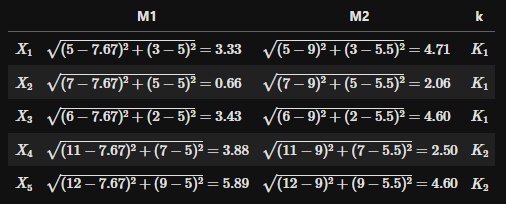
\includegraphics[width=1.0\textwidth]{images/kmeans_step_1.png}
    \caption{MAX\_ITER = 0}
    \label{fig:enter-label}
\end{figure}

Başlangıç adımında $K_1$ kümemiz Belge 1, Belge 2, Belge 4 belgelerinden; $K_2$ kümemiz Belge 3, Belge 5 belgelerinden oluşuyordu. Fakat ilk iterasyondan sonra görünüyorki Belge 3 $K_1$ kümesine, Belge 4 ise $K_2$ kümesine daha yakın. Dolayısıyla yeni kümelerimiz artık;

\begin{itemize}
    \item $K_1$ = Belge 1, Belge 2, Belge 3
    \item $K_2$ = Belge 4, Belge 5 olmuş oldu.
\end{itemize}

Şimdi yeni küme merkezlerimizi hesaplayalım.

\begin{itemize}
    \item $K_1 = [\frac{5 + 7 + 6}{3} = 6, \frac{3 + 5 + 2}{3} = 3.33]$
    \item $K_2 = [\frac{11 + 12}{2} = 11.5, \frac{7 + 9}{2} = 8]$, yeni küme merkezlerimiz bunlardır.
\end{itemize}

\begin{figure}[h]
    \centering
    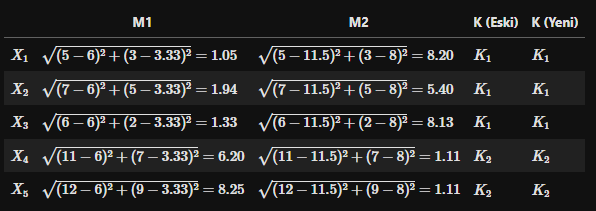
\includegraphics[width=1.0\textwidth]{images/kmeans_step_2.png}
    \caption{MAX\_ITER = 1}
    \label{fig:enter-label}
\end{figure}


Son adımdan da görüneceği gibi K (Eski) ve K (Yeni) sütunları birbirinin aynısı oldu. Yani nihai sonucu elde ettik. Bundan sonra iterasyon yapmamıza gerek yok. 


\subsubsection{Python Kodu}

\begin{lstlisting}[language=Python, caption=Scikit-learn'de KMeans örneği.]
import numpy as np
import pandas as pd
import random

class KMeans:
    def __init__(self, n_clusters=2, max_iter=300):
        # Olusturulacak kume sayisi (k)
        self.n_clusters = n_clusters
        # Maksimum iterasyon sayisi
        self.max_iter = max_iter
        # Kume merkezleri
        self.centroids = None

    def initialize_centroids(self, X):
        # Ilk olarak merkez rastgele secilir.
        centroids = [random.choice(X)]

        # "Euclidean Distance (Oklid mesafesi)" ile diger merkezler uzakliklara gore secilir. (K-Means++)
        for _ in range(1, self.n_clusters):
            # Her bir noktanin mevcut merkezlere olan minimum uzakligi hesaplanir.
            distances = np.min(np.linalg.norm(X - np.array(centroids)[:, np.newaxis], axis=2), axis=0)
            # Olasiliklar normalize edilir.
            distances /= np.sum(distances)

            # Uzaklik olasiliklarina gore yeni merkez secilir.
            next_centroid = X[np.random.choice(len(X), p=distances)]
            centroids.append(next_centroid)

        return np.array(centroids).astype("float32")

    def assign_clusters(self, X):
        # Her nokta en yakin merkeze atanir.
        distances = np.linalg.norm(X[:, np.newaxis] - self.centroids, axis=2).astype("float32")
        return np.argmin(distances, axis=1)

    def update_centroids(self, X, labels):
        # Her kumenin yeni merkezini hesaplanir.
        new_centroids = np.array([X[labels == i].mean(axis=0) if len(X[labels == i]) > 0 else self.centroids[i]
                                    for i in range(self.n_clusters)]).astype("float32")
        return new_centroids

    def fit(self, X):
        # Merkezler baslatilir.
        self.centroids = self.initialize_centroids(X)

        for _ in range(self.max_iter):
            # Her nokta en yakin merkeze atanir.
            labels = self.assign_clusters(X)

            # Yeni merkezler hesaplanir.
            new_centroids = self.update_centroids(X, labels)

            # Merkezler degismediyse islem tamamlanmistir.
            if np.allclose(self.centroids, new_centroids):
                break

            # Merkezler degistiyse yeni merkezler mevcut merkezlerin yerine atanir.
            self.centroids = new_centroids

    def predict(self, X):
        # Her veri noktasi icin en yakin merkezin indeksi alinir.
        labels = self.assign_clusters(X)
        # En yakin merkezin koordinatlari dondurulur.
        labels_coords = np.array([self.centroids[label] for label in labels]).astype("float32")
        return labels_coords, labels
\end{lstlisting}

\newpage

\subsection{MeanShift}
Mean Shift, veri noktalarını veri yoğunluğu temelinde kümelemek için kullanılır. Algoritma, veri noktalarını yoğunluk merkezlerine kaydırarak kümelemeyi gerçekleştirir. Mean Shift, veri yoğunluğuna dayalı olarak doğal kümeleri bulur.

\subsubsection{Çalışma Adımları}
\begin{itemize}
    \item Her veri noktası, başlangıçta kendisinin bir merkez olarak kabul edildiği bir yoğunluk merkezine atanır.
    \item Her bir veri noktası için yoğunluk merkezi hesaplanır. Yoğunluk merkezi, veri noktalarının yoğunluğunun maksimum olduğu noktadır.
    \item Her veri noktası, hesaplanan yoğunluk merkezi pozisyonuna kaydırılır.
    \item 2. ve 3. adımlar tekrar edilir, veri noktaları yoğunluk merkezlerine yaklaştıkça, yoğunluk merkezleri daha da hassaslaşır.
    \item Veri noktaları yoğunluk merkezlerine yaklaşmayı bıraktığında sonlanır. Her bir veri noktası son yoğunluk merkezi ile ilişkilendirilir.
\end{itemize}

\subsubsection{Hiperparametreler}

\begin{table}[h]
\centering
{\scriptsize\renewcommand{\arraystretch}{0.4}
{\resizebox*{\linewidth}{0.3\textwidth}{
\begin{tabular}{|p{3cm}|p{1cm}|p{1cm}|p{6cm}|}
\hline
Parametre & Type & Default & Açıklama \\ \hline
bandwidth & float & None & Bandwidth, yoğunluk merkezlerini hesaplamak için kullanılan pencerenin boyutunu belirler. Büyük bir bant genişliği, daha geniş yoğunluk merkezleri üretebilirken, küçük bir bant genişliği daha küçük ve hassas yoğunluk merkezleri üretebilir. Bandwidth, Mean Shift algoritmasının en önemli hiperparametrelerinden biridir ve doğru bir şekilde ayarlanmalıdır. \\ \hline


\end{tabular}
}}}
\end{table}

\subsubsection{Python Kodu}

\begin{lstlisting}[language=Python, caption=Scikit-learn'de MeanShift örneği.]
from sklearn.cluster import MeanShift
from sklearn.datasets import make_blobs
import matplotlib.pyplot as plt

# Veri olusturma
data, _ = make_blobs(n_samples=300, centers=4, cluster_std=1.0, random_state=42)

# Mean Shift modeli olusturma
model = MeanShift()  # Hiperparametreler belirtilmezse varsayilan degerler kullanilir

# Veriyi modele uydurma
labels = model.fit_predict(data)

# Sonuclari gorsellestirme
plt.scatter(data[:, 0], data[:, 1], c=labels, cmap='viridis')
plt.show()
\end{lstlisting}

\newpage

\subsection{MiniBatchKMeans}
MiniBatchKMeans, geleneksel K-Means kümeleme algoritması ile benzer bir yaklaşımı temel alır, ancak büyük veri kümeleri üzerinde daha hızlı çalışmak için bir örnekleme (mini-batch) tabanlı bir yaklaşım kullanır. Bu, büyük veri setlerini hızlı bir şekilde kümelemek için kullanışlıdır.

\subsection{Çalışma Adımları}
\begin{itemize}
    \item MiniBatchKMeans, rastgele seçilen bir alt örneklemi (mini-batch) kullanır.
    \item Mini-batch üzerinde K-Means algoritmasının adımları uygulanır.
    \item Mini-batch'ler sırayla kullanılır ve her bir mini-batch işlendikten sonra küme merkezleri güncellenir.
    \item İterasyonlar belirli bir duruma ulaştığında veya belirli bir iterasyon sayısına ulaştığında algoritma sonlanır.
\end{itemize}

\subsubsection{Hiperparametreler}

\begin{table}[h]
\centering
{\scriptsize\renewcommand{\arraystretch}{0.4}
{\resizebox*{\linewidth}{0.4\textwidth}{
\begin{tabular}{|p{3cm}|p{1cm}|p{1cm}|p{6cm}|}
\hline
Parametre & Type & Default & Açıklama \\ \hline
n\_clusters & int & 8 & Kümelerin sayısını belirler. Bu, kullanıcı tarafından belirlenen bir hiperparametredir. \\ \hline
batch\_size & int & 1024 & Her mini-batch'in boyutunu belirler. Daha büyük bir batch\_size, daha yüksek hesaplama maliyeti demektir. Mini-batch boyutunu seçerken bellek ve hesaplama gücü sınırlamalarını göz önünde bulundurmalısınız. \\ \hline
max\_iter & int & 100 & İterasyonların maksimum sayısını belirler. Algoritmanın ne kadar süre çalışacağını kontrol eder. \\ \hline
init & "k-means++", "random" & "k-means++" & Başlangıç merkezlerini seçme yöntemini belirler. \\ \hline

\end{tabular}
}}}
\end{table}

\subsubsection{Python Kodu}

\begin{lstlisting}[language=Python, caption=Scikit-learn'de MiniBatchKMeans.]
from sklearn.cluster import MiniBatchKMeans
from sklearn.datasets import make_blobs
import matplotlib.pyplot as plt

# Veri olusturma
data, _ = make_blobs(n_samples=300, centers=4, cluster_std=1.0, random_state=42)

# MiniBatchKMeans modeli olusturma
model = MiniBatchKMeans(n_clusters=4)  # Kume sayisini belirtin

# Veriyi modele uydurma
labels = model.fit_predict(data)

# Sonuclari gorsellestirme
plt.scatter(data[:, 0], data[:, 1], c=labels, cmap='viridis')
plt.show()
\end{lstlisting}

\newpage

\subsection{OPTICS}
OPTICS (Ordering Points To Identify the Clustering Structure), yoğunluk temelli kümeleme problemlerinde etkilidir. OPTICS, veri noktalarını sıralayarak kümeleme yapar ve doğal kümeleri ve yoğunluk tabanlı yapısını belirler.

\subsubsection{Hiperparametreler}

\begin{table}[h]
\centering
{\scriptsize\renewcommand{\arraystretch}{0.4}
{\resizebox*{\linewidth}{0.4\textwidth}{
\begin{tabular}{|p{3cm}|p{1cm}|p{1cm}|p{6cm}|}
\hline
Parametre & Type & Default & Açıklama \\ \hline
eps & float & None & Veri noktalarının bir yoğunluk merkezine erişilebilir kabul edilebilecek maksimum uzaklığı belirler. Bu eşik değeri, kümeleme sonuçlarını etkiler. \\ \hline
min\_samples & int & 5 & Bir yoğunluk merkezi olarak kabul edilebilecek minimum veri noktası sayısını belirler. Bu, bir yoğunluk merkezi olarak kabul edilmesi için veri noktalarının çevresinde en az kaç veri noktasının bulunması gerektiğini kontrol eder. \\ \hline

\end{tabular}
}}}
\end{table}

\subsubsection{Python Kodu}

\begin{lstlisting}[language=Python, caption=Scikit-learn'de OPTICS örneği.]
from sklearn.cluster import OPTICS
from sklearn.datasets import make_blobs
import matplotlib.pyplot as plt

# Veri olusturma
data, _ = make_blobs(n_samples=300, centers=4, cluster_std=1.0, random_state=42)

# OPTICS modeli olusturma
model = OPTICS()  # Hiperparametreler belirtilmezse varsayilan degerler kullanilir.

# Veriyi modele uydurma
model.fit(data)

# Sonuclari gorsellestirme
plt.scatter(data[:, 0], data[:, 1], c=model.labels_, cmap='viridis')
plt.show()
\end{lstlisting}

\newpage

\subsection{SpectralClustering}
Spectral Clustering, veri noktalarının benzerlik grafiği üzerinden kümeleme yapma yeteneğine sahiptir. Bu algoritma, veri noktalarının benzerlik matrisini kullanarak bir graf oluşturur ve bu grafiği kullanarak veri kümelemesi yapar.

\subsubsection{Çalışma Adımları}
\begin{itemize}
    \item Veri noktaları arasındaki benzerliği ölçen benzerlik matrisi oluşturulur. Benzerlik matrisi, bir grafı temsil eder. Her bir veri noktası bir düğüm ve benzerlikler arasındaki değerler ise kenarlar olarak düşünülür.
    \item Graf üzerinde Laplace matrisi hesaplanır. Laplace matrisi, grafın yapısını ve veri noktalarının bağlantılarını yakalar.
    \item Laplace matrisinin özdeğer ayrışımı (eigendecomposition) yapılır ve özdeğerler kullanılarak veri noktaları spektral uzayda temsil edilir.
    \item Elde edilen spektral uzayda k-means veya diğer kümeleme yöntemleri kullanılarak veri noktaları kümelere ayrılır.
\end{itemize}

\subsubsection{Hiperparametreler}

\begin{table}[h]
\centering
{\scriptsize\renewcommand{\arraystretch}{0.4}
{\resizebox*{\linewidth}{0.4\textwidth}{
\begin{tabular}{|p{3cm}|p{1cm}|p{1cm}|p{6cm}|}
\hline
Parametre & Type & Default & Açıklama \\ \hline
n\_clusters & int & 8 & Küme sayısını belirler. Hangi sayıyı seçeceğinizi veri yapısına ve analiz amacınıza bağlı olarak belirlemelisiniz. \\ \hline
affinity & str & "rbf" & Benzerlik matrisi hesaplama yöntemini belirler. Öklidyen uzaklık veya kosinüs benzerliği gibi farklı metrikler kullanılabilir. \\ \hline
n\_neighbors & int & 10 & Grafiği oluştururken her veri noktasının en yakın kaç komşusunu kullanacağınızı belirler. Bu, grafın yoğunluğunu ve bağlantılarını etkiler. \\ \hline
eigen\_solver & "arpack", "lobpcg", "amg" & "k-means++" & Özdeğer ayrışımını yaparken kullanılacak algoritmayı belirler. \\ \hline
\end{tabular}
}}}
\end{table}

\subsubsection{Python Kodu}

\begin{lstlisting}[language=Python, caption=Scikit-learn'de SpectralClustering örneği.]
from sklearn.cluster import SpectralClustering
from sklearn.datasets import make_blobs
import matplotlib.pyplot as plt

# Veri olusturma
data, _ = make_blobs(n_samples=300, centers=4, cluster_std=1.0, random_state=42)

# SpectralClustering modeli olusturma
model = SpectralClustering(n_clusters=4)  # Kume sayisini belirtin

# Veriyi modele uydurma
labels = model.fit_predict(data)

# Sonuclari gorsellestirme
plt.scatter(data[:, 0], data[:, 1], c=labels, cmap='viridis')
plt.show()
\end{lstlisting}

\newpage
\section{Cold Start}
Cold start, yeni bir öğe, kullanıcı veya durumla ilgili veri eksikliği veya sınırlı veri durumunda ortaya çıkar. Sistemlerin doğruluğunu ve etkinliğini olumsuz etkiler. Özellikle öneri sistemleri için kullanıcı deneyimini azaltabilir.

\begin{enumerate}
    \item \textbf{Cold User Start:} Yeni bir kullanıcı hakkında çok az veya hiç veri bulunmaması durumudur.
    \item \textbf{Cold Item Start:} Yeni bir öğe hakkında yeterince veri olmaması durumudur. Önlemek için "Content-based filtering" kullanılır.
\end{enumerate}

\newpage
\section{Conformal Prediction}
Belirsizlik tahmini yapmak için uyumluluk tahmini prensiplerini kullanan bir yaklaşımdır. Bir modelin tahminlerinin güvenirliliğini değerlendirmek ve belirsizlikleri hesaba katmak için kullanılır. Model eğitim verilerini kullanarak bir uyumluluk bölgesi oluşturur. Bu bölge, modelin eğitim verilerinde yakaladığı örüntüleri gösterir. Sınama verileri için bu uyumluluk bölgesine dayanarak bir tahmin yapılır. Böylece belirli bir güven düzeyinde tahminler yapılır.

\subsubsection{Inductive Conformal Predictors}
\begin{enumerate}
    \item Bir modelin eğitim verilerine dayanarak belirli bir güven düzeyinde uyumluluk tahmini yapar.
    \item Model, eğitim verilerindeki benzer örneklerin dağılımına dayanarak bir güven aralığı hesaplar.
    \item Her bir tahmin için güven aralığı belirlenir.
\end{enumerate}

\subsubsection{Aggregated Conformal Predictors}
\begin{enumerate}
    \item Birden fazla modelin çıktılarını bir araya getirerek daha güvenilir tahminler elde etmeyi amaçlar.
    \item Her bir modelin tahminleri, uyumluluk tahminine göre bir araya getirilir. Böylece toplu bir güven aralığı sağlanır.
\end{enumerate}

\subsubsection{Transductive Conformal Prediction}
\begin{enumerate}
    \item Her bir test örneği için, modelin oluşturduğu uyumluluk bölgesine dayanarak bir tahmin yapılır. Bu tahmin için test örneği yanında diğer eğitim örneklerini de kullanır.
\end{enumerate}

\newpage
\section{Cross Validation Methods}
Çapraz doğrulama, bir modelin performansını değerlendirmek için veri setini farklı parçalara böler ve her bir parça üzerinde modelin performansını değerlendirir. Bu yöntem, modelin gerçek dünya verilerine nasıl genelleme yapabileceğini daha güvenilir bir şekilde belirlemek için kullanılır. Çapraz doğrulama, aşırı uyum (overfitting) problemini önlemeye yardımcı olur ve modelin gerçek performansını daha doğru bir şekilde yansıtır.

\begin{enumerate}
    \item KFold
    \item Stratified KFold
    \item Repeated KFold
    \item Repeated Stratified KFold
    \item Leave One-Out
    \item Leave P-Out
    \item Time Series Split
\end{enumerate}

\newpage

\subsection{KFold}
Veriyi rastgele parçalara böler ve modeli eğitmek ve test etmek için bu parçaları kullanır. Veri setini daha iyi kullanarak eğitim yapılmasını sağlar. Yavaş olabilir.

\subsubsection{Çalışma Adımları}
\begin{enumerate}
    \item Veri kümesi K parçaya bölünür.
    \item K parçanın her biri sırasıyla test seti olarak kullanır. Diğer k-1 parçayı eğitim seti olarak kullanır. 
    \item Model K kez eğitilir ve test edilir.
    \item Her bir eğitim-test işlemi sonucunda elde edilen performans ölçümleri ortalanır.
\end{enumerate}

\begin{figure}[h]
    \centering
    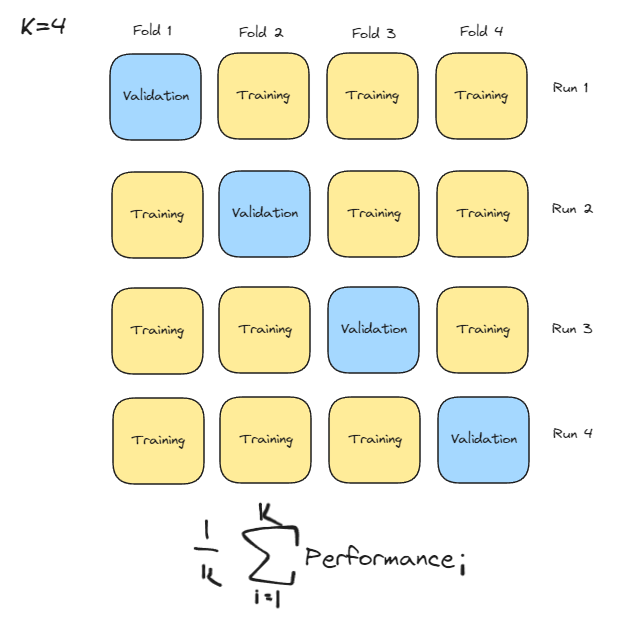
\includegraphics[width=0.8\textwidth]{images/kfold_structure.png}
    \caption{KFold.}
    \label{fig:enter-label}
\end{figure}

\subsubsection{Python Kodu}

\begin{lstlisting}[language=Python, caption=Scikit-learn'de KFold örneği.]
from sklearn.model_selection import KFold
from sklearn.linear_model import LinearRegression
import numpy as np

X = np.array([[1, 2], [3, 4], [5, 6], [7, 8]])
y = np.array([11, 12, 13, 14])

kf = KFold(n_splits=2)

for train_index, test_index in kf.split(X):
    X_train, X_test = X[train_index], X[test_index]
    y_train, y_test = y[train_index], y[test_index]
    
    model = LinearRegression()
    model.fit(X_train, y_train)
    
    score = model.score(X_test, y_test)
    print("Test seti skoru:", score)
\end{lstlisting}

\newpage

\subsection{Stratified KFold}
KFold gibi çalışır fakat her katmanın sınıf dağılımını korumak için sınıfları dengeli bir şekilde böler. Sınıf dengesizliği durumunda daha güvenilir sonuçlar sağlar. Sınıf dağılımını koruyarak her katmanda her sınıfın temsil edilmesini sağlar. Stratifikasyon her zaman mümkün olmayabilir.

\subsubsection{Çalışma Adımları}
\begin{enumerate}
    \item Veri kümesi k parçaya bölünür.
    \item Her bir parçanın sınıf dağılımını KFold gibi böler.
    \item Her parça, orijinal veri setindeki sınıf oranlarını yansıtacak şekilde oluşturulur.
    \item Model K kez eğitilir ve test edilir, her seferinde farklı bir parça test seti olarak seçilir.
\end{enumerate}

\begin{figure}[h]
    \centering
    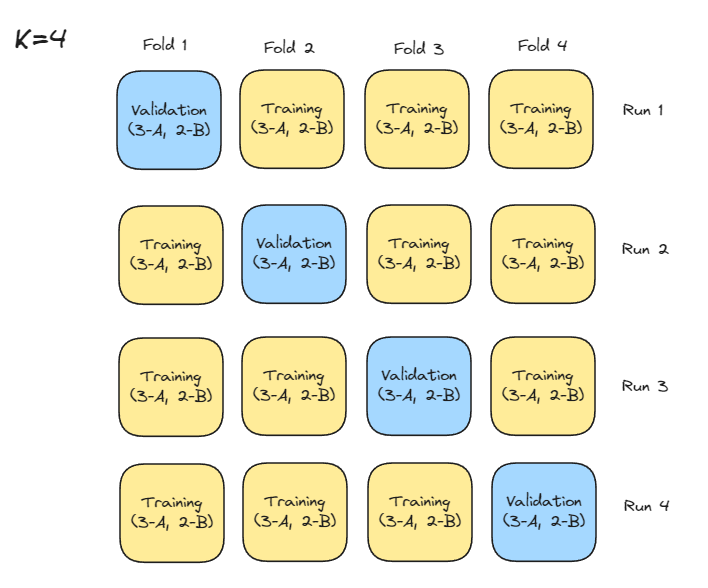
\includegraphics[width=0.8\textwidth]{images/stratified_kfold_structure.png}
    \caption{Stratified KFold.}
    \label{fig:enter-label}
\end{figure}

\subsubsection{Python Kodu}

\begin{lstlisting}[language=Python, caption=Scikit-learn'de Stratified KFold örneği.]
from sklearn.model_selection import StratifiedKFold
from sklearn.datasets import make_classification
from sklearn.linear_model import LogisticRegression

X, y = make_classification(n_samples=100, n_features=4, n_informative=2, n_redundant=0, random_state=42, n_classes=2)

skf = StratifiedKFold(n_splits=3)

for train_index, test_index in skf.split(X, y):
    X_train, X_test = X[train_index], X[test_index]
    y_train, y_test = y[train_index], y[test_index]
    
    model = LogisticRegression()
    model.fit(X_train, y_train)
    
    score = model.score(X_test, y_test)
    print("Test seti skoru:", score)
\end{lstlisting}

\newpage

\subsection{Repeated KFold}
Veri kümesini KFold yöntemiyle bölmenin tekrarlanabilir bir versiyonudur. Bir KFold çapraz doğrulama işlemini belirli bir sayıda tekrarlayarak daha güvenilir bir performans tahmini elde etmeyi amaçlar. Veri kümesi dengeli ise gereksiz olabilir.

\subsubsection{Çalışma Adımları}
\begin{enumerate}
    \item Veri kümesi k parçaya bölünür.
    \item Bu K parçayı kullanarak model eğitilir ve test edilir.
    \item İşlem belirli bir sayıda tekrarlanır.
    \item Her tekrarda farklı rastgele parçalar seçilir.
\end{enumerate}

\subsubsection{Python Kodu}

\begin{lstlisting}[language=Python, caption=Scikit-learn'de Repeated KFold örneği.]
from sklearn.model_selection import RepeatedKFold
from sklearn.datasets import make_regression
from sklearn.linear_model import LinearRegression

X, y = make_regression(n_samples=100, n_features=2, noise=0.1, random_state=42)

rkf = RepeatedKFold(n_splits=3, n_repeats=2)

for train_index, test_index in rkf.split(X):
    X_train, X_test = X[train_index], X[test_index]
    y_train, y_test = y[train_index], y[test_index]
    
    model = LinearRegression()
    model.fit(X_train, y_train)
    
    score = model.score(X_test, y_test)
    print("Test seti skoru:", score)
\end{lstlisting}

\newpage

\subsection{Repeated Stratified KFold}
StratifiedKFold'un tekrarlanabilir bir versiyonudur. Sınıflandırma problemlerinde kullanılan ve sınıf dengesini koruyarak veri setini tekrarlayan bir çapraz doğrulama tekniğidir.

\subsubsection{Çalışma Adımları}
\begin{enumerate}
    \item Veri kümesi StratifiedKFold gibi sınıf dengesini koruyarak K parçaya bölünür.
    \item Bu K parçayı kullanarak modeli eğitir ve test eder.
    \item İşlem belirli bir sayıda tekrarlanır.
    \item Her tekrarda farklı rastgele parçalar seçilir.
\end{enumerate}

\subsubsection{Python Kodu}

\begin{lstlisting}[language=Python, caption=Scikit-learn'de Repeated Stratified KFold örneği.]
from sklearn.model_selection import RepeatedStratifiedKFold
from sklearn.datasets import make_classification
from sklearn.ensemble import RandomForestClassifier

X, y = make_classification(n_samples=100, n_features=4, n_informative=2, n_redundant=0, random_state=42, n_classes=2)

rskf = RepeatedStratifiedKFold(n_splits=3, n_repeats=2, random_state=42)

for train_index, test_index in rskf.split(X, y):
    X_train, X_test = X[train_index], X[test_index]
    y_train, y_test = y[train_index], y[test_index]
    
    model = RandomForestClassifier()
    model.fit(X_train, y_train)
    
    score = model.score(X_test, y_test)
    print("Test seti skoru:", score)
\end{lstlisting}

\newpage

\subsection{Leave One-Out}
Veri setinin her bir örneğini sadece bir kez test seti olarak kullanarak gerçekleştirilir. Her bir veri noktası sırasıyla test edilirken geri kalanı eğitim seti olarak kullanılır.

\subsubsection{Çalışma Adımları}
\begin{enumerate}
    \item Veri kümesi içindeki her bir örnek sırayla test seti olarak seçilir.
    \item Seçilen örnek dışındaki tüm veri eğitim seti olarak kullanılır.
    \item Model, seçilen örneği test etmek ve performansını ölçmek için eğitilir.
    \item Bu işlem tüm veri noktaları için tekrarlanır.
\end{enumerate}

\begin{figure}[h]
    \centering
    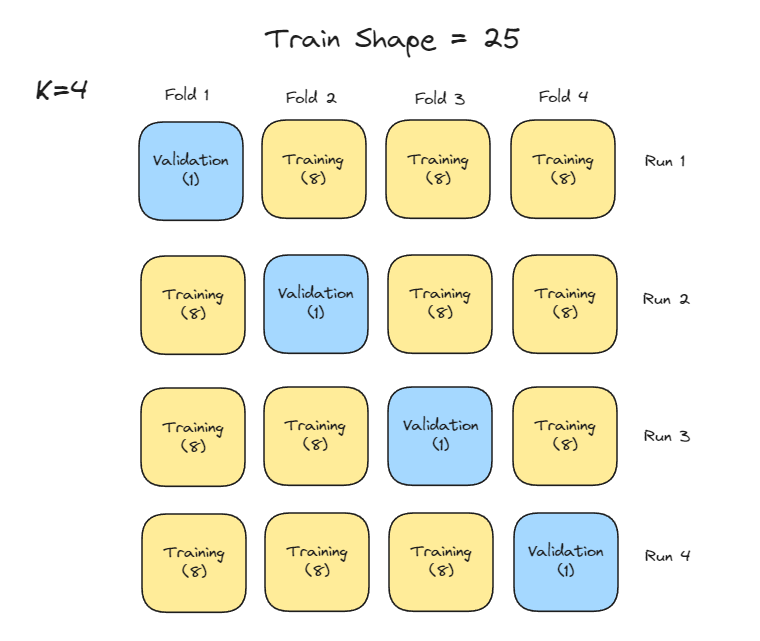
\includegraphics[width=0.8\textwidth]{images/leave_one_out_structure.png}
    \caption{Leave One-Out.}
    \label{fig:enter-label}
\end{figure}

\subsubsection{Python Kodu}

\begin{lstlisting}[language=Python, caption=Scikit-learn'de Leave One-Out örneği.]
from sklearn.model_selection import LeaveOneOut
from sklearn.datasets import load_iris
from sklearn.neighbors import KNeighborsClassifier

iris = load_iris()
X = iris.data
y = iris.target

loo = LeaveOneOut()

accuracies = []
for train_index, test_index in loo.split(X):
    X_train, X_test = X[train_index], X[test_index]
    y_train, y_test = y[train_index], y[test_index]
    
    model = KNeighborsClassifier()
    model.fit(X_train, y_train)
    
    accuracy = model.score(X_test, y_test)
    accuracies.append(accuracy)

mean_accuracy = sum(accuracies) / len(accuracies)
print("Ortalama dogruluk:", mean_accuracy)
\end{lstlisting}

\newpage

\subsection{Leave P-Out}
Her bir iterasyonda P öğeyi test seti olarak kullanarak gerçekleştirilir. LOO (Leave One-Out) ve KFold'un genelleştirilmiş bir versiyonudur. LOO, P=1 olduğunda Leave P-Out'a eşittir.

\subsubsection{Çalışma Adımları}
\begin{enumerate}
    \item Veri kümesinde P öğeyi test seti olarak bırakır, geri kalanını eğitim seti olarak kullanır.
    \item Model, test setindeki öğeleri tahmin etmek ve performansını ölçmek için eğitilir.
    \item Bu işlem veri kümesindeki her bir P öğesi için tekrarlanır.
\end{enumerate}

\begin{figure}[h]
    \centering
    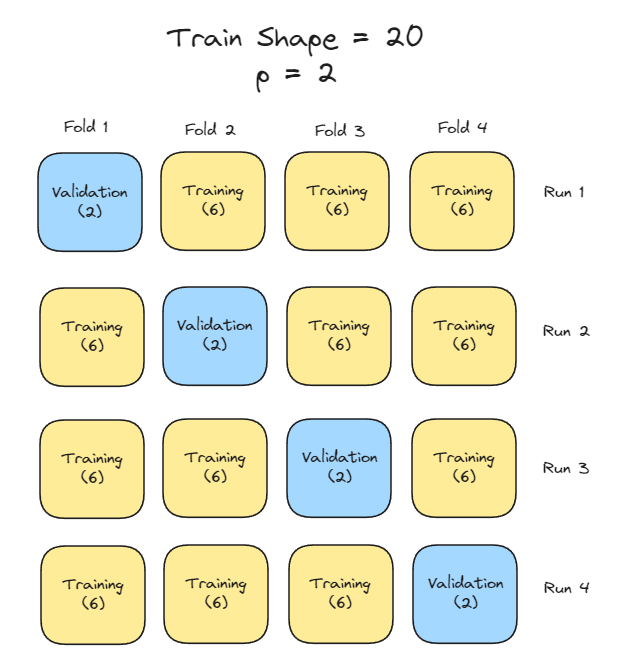
\includegraphics[width=0.8\textwidth]{images/leave_p_out_structure.png}
    \caption{Leave P-Out.}
    \label{fig:enter-label}
\end{figure}

\subsubsection{Python Kodu}

\begin{lstlisting}[language=Python, caption=Scikit-learn'de Leave P-Out örneği.]
from sklearn.model_selection import LeavePOut
from sklearn.datasets import load_iris
from sklearn.neighbors import KNeighborsClassifier

iris = load_iris()
X = iris.data
y = iris.target

lpout = LeavePOut(p=2)

accuracies = []
for train_index, test_index in lpout.split(X):
    X_train, X_test = X[train_index], X[test_index]
    y_train, y_test = y[train_index], y[test_index]
    
    model = KNeighborsClassifier()
    model.fit(X_train, y_train)
    
    accuracy = model.score(X_test, y_test)
    accuracies.append(accuracy)

mean_accuracy = sum(accuracies) / len(accuracies)
print("Ortalama dogruluk:", mean_accuracy)
\end{lstlisting}

\newpage

\subsection{Time Series Split}
Zaman serisi veri setlerinde kullanılan çapraz doğrulama yöntemlerinden biridir. Zaman serileri için veriyi bölme ve çapraz doğrulama yapma işlemidir.

\subsubsection{Çalışma Adımları}
\begin{enumerate}
    \item Veri, kronolojik sıraya göre (zaman bileşeni) parçalara bölünür.
    \item Her bir bölüm, eğitim ve test setleri olarak kullanılır.
    \item Örneğin, ilk k-1 bölüm eğitim seti, k. bölüm test seti olarak kullanılabilir.
    \item Bu işlem bir döngü içinde tekrarlanarak farklı eğitim ve test setleri elde edilir.
\end{enumerate}

\begin{figure}[h]
    \centering
    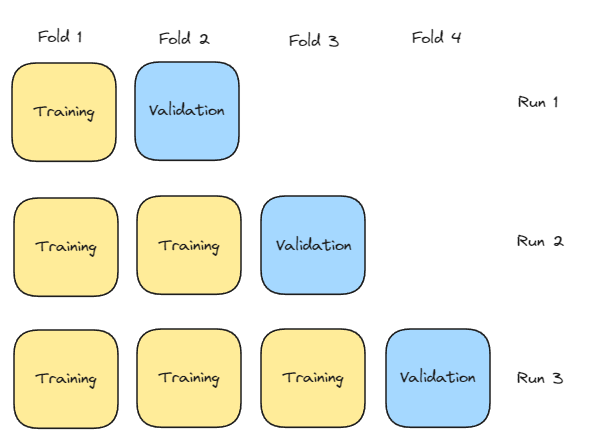
\includegraphics[width=0.8\textwidth]{images/time_series_split_structure.png}
    \caption{Time Series Split.}
    \label{fig:enter-label}
\end{figure}

\subsubsection{Python Kodu}

\begin{lstlisting}[language=Python, caption=Scikit-learn'de Time Series Split örneği.]
from sklearn.model_selection import TimeSeriesSplit
import numpy as np

time_series = np.array([1, 2, 3, 4, 5, 6, 7, 8, 9, 10])

tscv = TimeSeriesSplit(n_splits=3)

for train_index, test_index in tscv.split(time_series):
    train_data, test_data = time_series[train_index], time_series[test_index]
    
    print("Egitim seti:", train_data)
    print("Test seti:", test_data)
    print("------")
\end{lstlisting}

\newpage
\section{Data Leakage}
Veri sızıntısı, bir makine öğrenimi modelinin eğitim sürecinde yanıltıcı bilgilerle karşılaşmasına ve bu nedenle gerçek dünya verilerinde beklenmedik hatalı sonuçlar üretmesine neden olur. Bu durum, modelin genellikle eğitim seti içinde olmayan bilgilere dayalı kararlar almasına yol açabilir. Veri sızıntısı, modelin yanıltıcı şekillerde yüksek doğruluk oranlarına ulaşmasına veya yanlış sonuçlar üretmesine neden olabilir. Modelin öğrenmemesi gereken bir şeyi öğrenmesidir. Aşağıdaki durumlar örnektir;

\begin{enumerate}
    \item Eksik verilerin veri setinin tümünü kullanarak (train-test ayırmadan) mean/mode/median ile doldurulması.
    \begin{lstlisting}[language=Python]
    df['col1'].fillna(df['col1'].mean(), inplace=True)
    \end{lstlisting}
    \item Scale ederken veri setinin tümünün kullanılması.
    \begin{lstlisting}[language=Python]
    X_scaled = StandardScaler().fit_transform(X)
    \end{lstlisting}
    \item Bazı metodların amacı dışında kullanımı.
    \begin{lstlisting}
    # LabelEncoder sadece hedef degisken icin kullanilmalidir. Train setinde bunun yerine OrdinalEncoder kullanilmalidir.
    le = LabelEncoder()
    X_train['col1] = le.fit_transform(X_train['col1']

    # OrdinalEncoder train-test ayrimi sonrasi kullanilmalidir.
    ord = OrdinalEncoder(encoded_missing_value=-1)
    X_train['col1] = ord.fit_transform(X_train['col1']
    \end{lstlisting}
    \item Over/Under Sampling işlemlerinde veri setinin tümünün kullanılması (train-test ayırmadan)
    \begin{lstlisting}[language=Python]
    X_resampled, y_resampled = smote.fit_resample(X, y)
    \end{lstlisting}
\end{enumerate}

\newpage

\section{Decision Tree}
Karar ağacı, bir veri setini, bir dizi karar uygulayarak daha küçük kümelere bölmek için kullanılan bir yapıdır. Karar ağacında ilk bölünmenin başladığı yere kök, dalların uzaması ile gelişen kısımlara düğüm, alt uçlara ise yaprak denir. Karar ağaçları, en iyi bölünmeyi seçmek için farklı kriterler kullanır. Daha uzun ağaçlar yerine daha kısa ağaçlar tercih edilir.  Düğümler:
\begin{enumerate}
    \item \textbf{Internal Node:} Özelliğin adı
    \item \textbf{Branch:} Bir üstteki özelliğin değeri
    \item \textbf{Leaf Node:} Tahmin Sınıfı
\end{enumerate}

\begin{figure}[h]
    \centering
    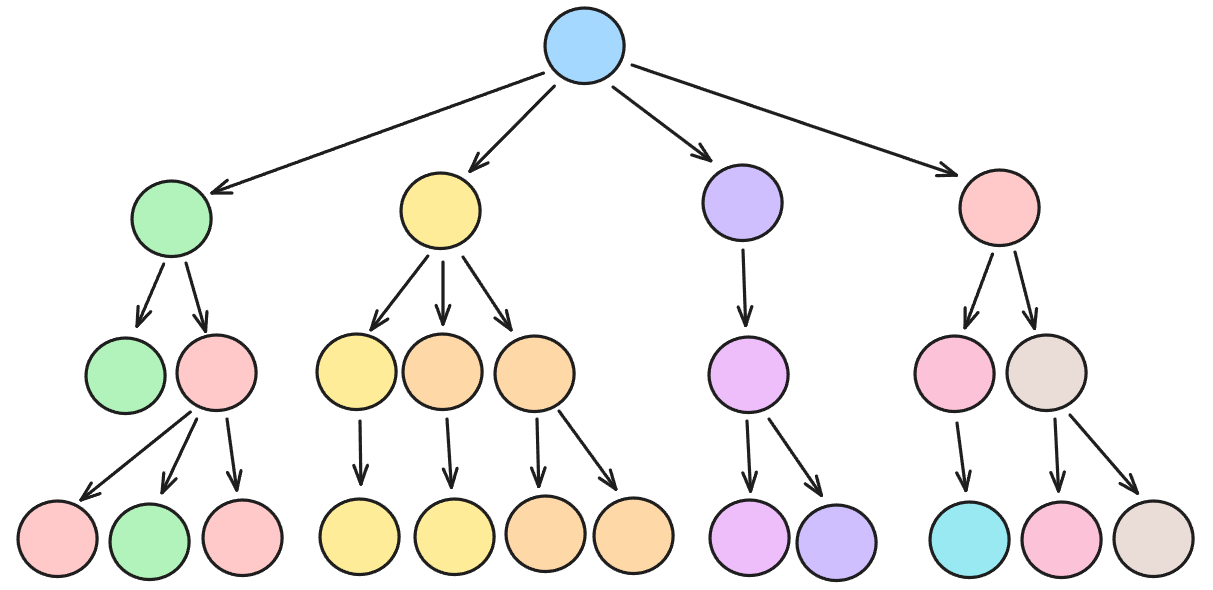
\includegraphics[width=1\textwidth]{images/decision_tree_structure.png}
    \caption{Karar ağacı.}
    \label{fig:enter-label}
\end{figure}

En yaygın olarak kullanılan algoritmalar.
\begin{enumerate}
    \item \textbf{Bilgi Kazancı (Information Gain):} Bir düğümün bölünmesinin ne kadar bilgi kazandıracağını ölçer. Bilgi kazancı, her alt düğümün belirli bir özellikle ne kadar homojen olduğunu gösteren bir metriktir. Bilgi kazancı, bir özellikle yapılan bölünmenin önceki duruma göre ne kadar daha az belirsizlik (bilgi eksikliği) getirdiğini ölçer. Bu, ağacın daha homojen alt gruplara bölünmesine ve iyi tahminler yapmasına yardımcı olur. Sırasıyla şu adımlar izlenir:
    \item \textbf{Entropi (Entropy):} Bir veri kümesinin ne kadar homojen veya heterojen olduğunu ölçen bir kavramdır. Daha yüksek entropi, daha fazla belirsizlik veya bilgi eksiliği anlamına gelir. Entropi şu formülle hesaplanır: E(S) = -p1 * log2(p1) - p2 * log2(p2) - ... - pk * log2(pk), burada p1, p2, ..., pk, S'deki her sınıfın olasılıklarıdır.
    \item \textbf{Dallanma (Split):} Bir özellik seçilir ve veri kümesi bu özelliğe göre alt gruplara bölünür. Her alt grup için entropi hesaplanır ve bu alt grupların ağırlıklı ortalaması (weighted average) alınır. Çok sayıda farklı kategorik değer alabilen özelliklerde Information Gain yöntemi etkili olmaz.
    \item \textbf{Jini Indeksi (Gini Index):} Bir düğümün homojenliğini ölçer. Daha küçük bir jini indeksi, daha homojen bir düğümü temsil eder.
\end{enumerate}

Pruning (Budama): Karar ağacında tahmine yeterince katkı yapmayan dallarda tahmin edici değişkenlerin modelden çıkarılması işlemidir. Post ve Pre olarak ikiye ayrılır. Prepruning, tahmin edici değişkenleri teker teker ele alarak modelin tahmin gücü için hangisinin etkili olacağı kararlaştırılarak adım adım dallanmaların ilerletilmesidir. Postpruning, tamamlanmış bir karar ağacından modele katkı yapmayan dalların tespit edilip modelden çıkarılmasıdır.

\subsection{Çalışma Adımları}
\begin{enumerate}
    \item Özellikler ve hedef değişken belirlenir.
    \item Ağacın kök düğümü seçilir ve veriler bu düğümde belirli bir özelliğe göre bölünür. Ardından, her alt düğüm için aynı adım tekrarlanır.
    \item Düğümler, en iyi bölünme kriterine göre alt düğümlere bölünür. Bölünme kriterleri genellikle bilgi kazancı, gini indeksi veya ortalama hata gibi metrikler kullanılarak belirlenir.
    \item Ağaç gereğinden fazla dallanma yapabilir. Bu nedenle gereksiz dallar kaldırılmaldır. (pruning)
    \item Yeni veriler için tahminler yapılır.
\end{enumerate}

\subsection{Avantajları}
\begin{enumerate}
    \item Yorumlaması kolaydır.
    \item Kullanılan ağaçlar görselleştirilebilir (sklearn.tree.plot\_tree()).
    \item Değişken seçimi yapabilir.
    \item Maaliyeti kullanılan veri boyutu ile logaritmiktir.
\end{enumerate}

\subsection{Dezavantajları}
\begin{enumerate}
    \item Overfitting sorunu. Budama işlemi ile önlenebilir.
    \item Heterojen veri üzerinde iyi performans göstermez.
    \item Yalnızca tek bir özellikle ilişkilendirilen ikinci sıra bağımlılıkları yakalayamaz.
\end{enumerate}

\newpage

\subsection{Hiperparametreler}
\begin{table}[h]
\centering
{\scriptsize\renewcommand{\arraystretch}{0.5}
{\resizebox*{\linewidth}{0.5\textwidth}{
\begin{tabular}{|p{3cm}|p{1cm}|p{1cm}|p{6cm}|}
\hline
Parametre & Type & Default & Açıklama \\ \hline
criterion & "gini", "entropy", "log\_loss" & "gini" & Ağaç oluşturma yöntemidir. \\ \hline
max\_depth & int & None & Ağacın maksimum derinliğini temsil eder. Değer verilmezse limitsiz olur. Overfitting'i önlemek için küçük bir değer girilmelidir. \\ \hline
min\_samples\_split & int/float & 2 & Bir düğümün bölünmeden önceki sahip olması gereken minimum örnek sayısıdır. \\ \hline
min\_samples\_leaf & int/float & 1 & Bir yaprağın sahip olması gereken minimum örnek sayısıdır. \\ \hline
min\_weight\_fraction\_leaf & float & 0 & Ağırlıklı örneklerin, toplam örnekler içerisindeki oranını temsil eder. \\ \hline
max\_leaf\_nodes & int & None & Maksimum yaprak sayısıdır. Overfitting'i engellemek için kullanılır. \\ \hline
max\_features & int/float, "auto", "sqrt", "log2" & None & En iyi bölünme için aranacak feature sayısıdır. \\ \hline

\end{tabular}
}}}
\end{table}

\newpage
\section{Discretization}

\subsection{Equal Width Discretization}
Veri değerlerini belirli genişlik alanlarına bölen bir veri ön işleme tekniğidir. Sürekli bir veri kümesini belirli bir sayıda aralığa (bin) bölerken değerlerin minimum ve maksimum değerleri kullanarak her aralığın genişliğini sabit tutar. Veride çok sayıda farklı değer varsa, bilgi kaybına neden olabilir.

\begin{lstlisting}[language=Python, caption=Scikit-learn ve feature\_engine örneği.]
# scikit
ewd = KBinsDiscretizer(n_bins=10, encode='ordinal', strategy='uniform')
ewd.fit(X_train[['column_name']])

# feature_engine
ewd = EqualWidthDiscretiser(bins=10, variables = ['column_name'])
ewd.fit(X_train)
\end{lstlisting}

\subsection{Equal Frequency Discretization}
Veri değerlerini belirli bir frekansta eşit sayıda öğe içeren gruplara bölen bir veri ön işleme tekniğidir. Veri değerleri sıralanır ve belirlenen grup sayısına göre her bir grup eşit sayıda veri öğesini içerecek şekilde oluşturulur.

\begin{lstlisting}[language=Python, caption=Scikit-learn ve feature\_engine örneği.]
pd.cut(x = X_train['column_name'], bins=intervals)
# scikit
efd = KBinsDiscretizer(n_bins=10, encode='ordinal', strategy='quantile')
efd.fit(X_train[['column_name']])

# feature_engine
efd = EqualFrequencyDiscretiser(q=10, variables = ['column_name'])
efd.fit(X_train)
\end{lstlisting}

\subsection{Arbitrary Interval Discretization}
Kullanıcı tarafından belirlenen özel aralıklar veya gruplar ile veri değerlerini gruplara ayırır. Yanlış sınır değerleri sonuçları etkileyebilir.

\subsection{K-Means Discretization}
K-Means kullanarak veri kümesini gruplara ayırır. K-Means veri noktalarını belirli bir sayıda küme merkezi etrafında kümelemek için kullanılır.

\begin{lstlisting}[language=Python, caption=Scikit-learn örneği.]
# scikit
kbins = KBinsDiscretizer(n_bins=10, encode='ordinal', strategy='kmeans')
kbins.fit(X_train[['column_name']])
\end{lstlisting}

\newpage
\section{Dummy}
Bir benchmark olarak veya başlangıç noktası olarak karmaşık modellerle karşılaştırma yapmak için bir referans olarak kullanılır. Girdi özelliklerini göz ardı ederek tahminler yapar.

\subsection{Hiperparametreler}
\begin{table}[h]
\centering
{\scriptsize\renewcommand{\arraystretch}{0.4}
{\resizebox*{\linewidth}{0.25\textwidth}{
\begin{tabular}{|p{3cm}|p{1cm}|p{1cm}|p{6cm}|}
\hline
Parametre & Type & Default & Açıklama \\ \hline
strategy & "gini", "entropy", "log\_loss" & "prior" & "most\_frequent": Her zaman en sık görülen sınıf etiketini döndürür. \\ \hline
random\_state & int & None & "uniform" her sınıf için eşit olarak tahminler üretir. \\ \hline
constant & int & None & "constant" sabit bit etiket tahmin eder. \\ \hline

\end{tabular}
}}}
\end{table}

\newpage

\section{ElasticNet}
L1 (Lasso) ve L2 (Ridge) düzenlemesinin bir kombinasyonunu kullanır. L1 ve L2 düzenleme terimlerini kontrol etmek için "alpha" parametresini kullanır. Alpha = 0 ise L2 uygulanır, böylece ElasticNet, Ridge regresyonuna dönüşür. Alpha = 1 ise L1 uygulanır, böylece ElasticNet, Lasso regresyonuna dönüşür.

\begin{table}[h]
\centering
{\scriptsize\renewcommand{\arraystretch}{0.1}
{\resizebox*{\linewidth}{0.2\textwidth}{
\begin{tabular}{|p{3cm}|p{1cm}|p{1cm}|p{6cm}|}
\hline
Parametre & Type & Default & Açıklama \\ \hline
alpha & float & 1.0 & L1 ve L2 regularizasyon birleşimini kontrol eder. \\ \hline
l1\_ratio & float & 0.5 & L1'in dağılımı. \\ \hline
max\_iter & int & 1000 & Optimizasyon algoritmasının maksimum iterasyon sayısı. \\ \hline
tol & float & 1e-4 & Optimizasyon algoritmasının toleransı. \\ \hline

\end{tabular}
}}}
\end{table}

\newpage
\section{Encoding}

\subsection{One Hot Encoding}
Kategorik verileri sayısal verilere dönüştürmek için kullanılan bir kodlama tekniğidir. Her bir kategorik değer, ayrı bir sütun olarak temsil edilir ve bu sütunlardaki değerler 1 veya 0 olarak kodlanır. Genellikle kategorik değişkenlerin sınırlı sayıda ve sıralı olmayan durumlarda tercih edilir. Çok sayıda benzersiz değer içeren veya yüksek kardinaliteye (yüksek sayıda farklı değer) içeren kategorik değişkenlerde uygulanırsa ortaya çıkacak olan çok fazla sütun veri setinin boyutunu artırabilir ve modelin karmaşıklığını artırabilir.

\begin{lstlisting}[language=Python, caption=Scikit-learn'de OneHotEncoding örneği.]
pd.get_dummies(X_train[cat_cols], drop_first=True)

# scikit
encoder = OneHotEncoder(categories='auto', drop='first', sparse=False)
encoder.fit(X_train[cat_cols])

# feature_engine
enc = OneHotCategoricalEncoder(top_categories=None, drop_last=True)
ohe_enc.fit(X_train)
\end{lstlisting}

\subsection{Ordinal Encoding}
Kategorik değerleri sıralı veya derecelendirilebilir olarak kabul eder ve bu sıralamayı temsil etmek üzere sayısal değerlerle kodlar. Veri setinin boyutunu artırmaz. Kategorik değişkenlerin sırasını korur. Kategorik değişkenler arasındaki eşit aralıklar olduğu varsayımına dayanır fakat bu her zaman doğru olmayabilir.

\begin{lstlisting}[language=Python, caption=Scikit-learn'de OrdinalEncoding örneği.]
ordinal_mapping = {k: i for i, k in enumerate(X_train['column_name'].unique(), 0)}
X_train['column_name'] = X_train['column_name'].map(ordinal_mapping)

# scikit
ord_encoder = OrdinalEncoder()
ord_encoder.fit(X_train[cat_cols])

# feature_engine
ord_encoder = OrdinalCategoricalEncoder(encoding_method='arbitrary', variables=cat_cols)
ord_encoder.fit(X_train)
\end{lstlisting}

\subsection{Count Encoding}
Her bir kategorik değer, o değerim verinde kaç kez tekrarlandığına bağlı olarak bir sayı ile kodlanır. Kategorik değişkenlerin sıklığına dayalı bilgiyi korur ve sıklıkla tekrarlanan değerlere daha yüksek sayısal değerler atar. Ancak veri setindeki bir değer çok fazla tekrarlanmıyorsa veya nadirse, bu yöntem o değeri temsil eden sayıyı düşük bir sayıda atayabilir. Bu durumda, nadir sınıflar için modelin performansını düşürebilir.

\begin{lstlisting}[language=Python, caption=Scikit-learn'de CountEncoding örneği.]
f_map = (X_train['column_name'].value_counts() / len(X_train) ).to_dict()
X_train['column_name'] = X_train['column_name'].map(f_map)

# feature_engine
count_encoder = CountFrequencyCategoricalEncoder(encoding_method='count', variables=None)
count_encoder.fit(X_train)
\end{lstlisting}

\subsection{Label Encoding}
Hedef kategorik değişkenin sayısal değerlere dönüştürülmesidir.

\begin{lstlisting}[language=Python, caption=Scikit-learn'de LabelEncoding örneği.]
le = LabelEncoder()
le.fit(X_train)
\end{lstlisting}

\subsection{Weights of Evidence Encoding (WOE)}
Her bir kategorik değeri, o kategoriye ait olasılığı hedef değişkenin iki farklı durumu arasındaki olasılık oranına dönüştürür. Bu oran, hedef değişkenin o kategoriye ait olduğu durumun olasılığını o kategorinin olmadığı durumun olasılığına böler. Hedef değişkenin binary olması gerekir. Kategoriler arasında çok az sayıda veri noktası olduğunda iyi sonuç vermez.

\begin{lstlisting}[language=Python, caption=Scikit-learn'de WOE örneği.]
# feature_engine
woe_encoder = WoERatioCategoricalEncoder(encoding_method='woe', variables=['column_name'])
woe_encoder.fit(X_train, y_train)
\end{lstlisting}

\subsection{Dummy Encoding}
One Hot Encoding'e benzer fakat OHE'de n farklı sınıf için n sütun varken Dummy Encoding'de n farklı sütun için n-1 adet sütun bulunur. Sütunlardan biri rastgele düşürülür. Örneğin 4 sınıftan oluşan bir sütuna OHE işlemi yaptığımızı düşünelim. OHE'de sınıfı temsil etmek için her satırda mutlaka "1" değeri bulunur. Dummy Encoding'de ise bir sütun tamamen sıfırlarla ifade edilir.

\begin{lstlisting}
# One Hot Encoding
ohe_arr = [
    [1, 0, 0, 0], # A class
    [0, 1, 0, 0], # B class
    [0, 0, 1, 0], # C class
    [0, 0, 0, 1]  # D class
]

# Dummy Encoding
de_arr = [
    [1, 0, 0], # A class
    [0, 1, 0], # B class
    [0, 0, 1], # C class
    [0, 0, 0]  # D class
]
\end{lstlisting}

\subsection{Effect Encoding}
Dummy Encoding'e benzer fakat bir sütun tamamen "0" yerine "-1" ile temsil edilir.

\begin{lstlisting}
# Dummy Encoding
de_arr = [
    [1, 0, 0], # A class
    [0, 1, 0], # B class
    [0, 0, 1], # C class
    [0, 0, 0]  # D class
]

# Effect Encoding
ee_arr = [
    [1, 0, 0],    # A class
    [0, 1, 0],    # B class
    [0, 0, 1],    # C class
    [-1, -1, -1]  # D class
]
\end{lstlisting}

\newpage
\section{Extra Trees}
Extremely Randomized Trees, ağaçların oluşturulması sırasında rastgelelik kullanarak bir dizi karar ağacı oluşturur ve bu ağaçların tahminlerini bir araya getirerek sonuçları üretir. Diğer ağaç tabanlı yöntemlerden farkı, ağaçların oluşturulması ve eğitim sürecindeki rastgelelik derecesinin daha yüksek olmasıdır.

\subsection{Çalışma Adımları}
\begin{itemize}
    \item Her bir ağaç oluşturulurken, özelliklerden rastgele bir alt küme seçilir.
    \item Her özellik için rastgele bir eşik değeri seçilir.
    \item Rastgele özellik ve eşik değerleri kullanılarak karar ağaçları oluşturulur. Maksimum derinliğe ulaşana kadar büyütülür.
    \item Bootstrap ile her ağacın farklı bir eğitim veri setiyle eğitilmesi sağlanır.
    \item Tüm ağaçlar üzerinde tahminler yapılır ve bu tahminler bir araya getirilerek modelin tahminleri üretilir. Sınıflandırma için en sık görülen tahmin alınır. Regresyon için tahminlerin ortalaması alınır.
\end{itemize}

\subsection{Hiperparametreler}
\begin{table}[h]
\centering
{\scriptsize\renewcommand{\arraystretch}{0.4}
{\resizebox*{\linewidth}{0.4\textwidth}{
\begin{tabular}{|p{3cm}|p{1cm}|p{1cm}|p{6cm}|}
\hline
Parametre & Type & Default & Açıklama \\ \hline
n\_estimators & int & 100 & Oluşturulacak ağaç sayısı. \\ \hline
max\_depth & int & None & Oluşturulacak ağaçların maksimum derinliği. Fazla olması modelin karmaşıklığını ve aşırı uyumu artırabilir. \\ \hline
min\_samples\_split & int & 2 & Bir iç düğümün ikiye bölünmeden önce kaç örneğe sahip olması gerektiği. \\ \hline
min\_samples\_leaf & int & 1 & Bir yaprak düğümünün en az kaç örneğe sahip olması gerektiği. \\ \hline
max\_features & "sqrt", "log2", float & "sqrt" & Her bir ağaçta kullanılacak maksimum özellik sayısı.  sqrt, len(n\_features). log2, log2(n\_features) \\ \hline
bootstrap & bool & None & Bootstrap örneklemlerinin kullanılıp kullanılmayacağını belirler. \\ \hline

\end{tabular}
}}}
\end{table}

\newpage
\section{Sampling Metodları}
Veri analizi ve makine öğrenimi projelerinde, dengesiz veri setleri sıkça karşılaşılan bir sorundur. Özellikle sınıflandırma problemlerinde, nadir sınıfların fazla sınıflara göre daha az örneklenmiş olması, modelin yanlış sonuçlar üretmesine neden olabilir. İşte bu durumda, oversampling ve undersampling gibi teknikler devreye girer.

Oversampling, nadir sınıflara ait örnekleri çoğaltarak veya yeniden örnekleme yaparak veri setinin dengesini sağlama işlemidir. Bu yöntem, nadir sınıfların temsil edilme oranını artırarak modelin daha dengeli bir şekilde eğitilmesini sağlar. Undersampling, fazla sınıflara ait örnekleri azaltarak veya örnekleri rastgele seçerek veri setinin dengesini sağlama işlemidir. Bu yöntem, fazla sınıfların temsil edilme oranını azaltarak veri setini daha dengeli hale getirir. Undersampling, modelin dengeli bir şekilde eğitilmesini sağlayabilir, ancak nadir sınıfların temsil edilme oranını azaltma riski taşır.

\begin{itemize}
    \item Dengesiz sınıf dağılımı düşük tespit oranına (recall score) yol açar.
    \item Örneklem arttırma (oversampling), örneklem azaltma (undersampling)
    \item Çoğunluk (majority), azınlık (minority)
\end{itemize}

Under Sampling Metodları
\begin{enumerate}
    \item Dönüştürülmüş Veri Seti Üzerinden Örneklem Seçen Metodlar
    \begin{enumerate}
        \item \textbf{Near Miss Undersampling:} Çoğunluk sınıfın azınlık sınıflara uzaklığına göre bu örneklemleri seçen bir örneklem azaltma metodudur.
        \item \textbf{Condensed Nearest Neighbors Rule:} CNN, KNN algoritmasının memory ihtiyacını azaltması için üretildi.
    \end{enumerate}
    \item Silinecek Örnekleri Seçen Metodlar
    \begin{enumerate}
        \item \textbf{Tomek Links:} Her bir sınıftan en yakın Öklid uzaklığına sahip birer tane örnek ile pair (çift) duruma gelmesini kural olarak koyar ve bu sınıflar arası oluşan çiftler Tomek linkler olarak adlandırılır.
        \item \textbf{Edited Nearest Neighbors Rule:} Kısa adı ENN. Veri setindeki belirsiz, gürültülü örnekleri ortadan kaldırmak için kullanılır. Veriden mümkün olduğunda az bilgi kaybına yol açarak yoğunluk sınıfını azaltması sağladığı en büyük faydadır.
    \end{enumerate}
    \item Hibrit Metodlar
    \begin{enumerate}
        \item \textbf{One Sided Selection:} Kısa adı OSS. Tomek Link ve CNN rule metodlarını kombinleyen bir metoddur. Tomek linklerinin sınırda ve gürültülü tüm veri örneklerini kaldırmasıyla oluşturduğu alt kümenin ardından CNN karar sınıfından uzaktaki çoğunluk sınıfı örneklerini veri setinden kaldırır.
        \item \textbf{Neighborhood Cleaning Rule:} CNN ve ENN metodlarını kombinleyen bir metoddur.
    \end{enumerate}
\end{enumerate}

Over Sampling Metodları

\begin{enumerate}
    \item Rastgele Oversampling
    \begin{enumerate}
        \item \textbf{Rastgele Tekrarlı Örnekleme (Random Oversampling):} Azınlık sınıftaki örnekleri rastgele seçerek artırır.
        \item \textbf{Rastgele SMOTE (Random SMOTE):} SMOTE yöntemini temel alır ve sentetik örnekler oluşturur, ancak bu işlemde rastgele seçilen örnekler kullanılır.
    \end{enumerate}
    \item Sentetik Oversampling
    \begin{enumerate}
        \item \textbf{SMOTE:} Azınlık sınıfındaki örnekleri kullanarak sentetik örnekler oluşturur.
        \item \textbf{ADASYN (Adaptive Synthetic Sampling):} Örneklerin yoğunluğuna göre sentetik örnekler üretir, özellikle azınlık sınıfındaki zor örnekler üzerinde odaklanır.
        \item \textbf{Borderline-SMOTE:} Sınıf sınırında yer alan örnekler üzerine odaklanır ve sentetik örnekler bu sınıflarda oluşturulur.
    \end{enumerate}
\end{enumerate}

\newpage

\subsection{SMOTE (Synthetic Minority Over-Sampling Technique)}
Azınlık sınıfındaki her bir örneğe rastgele seçilen komşuları arasında bir veya birkaç benzer örnek oluşturur. Bu benzer örnekler arasında yeni sentetik örnekler oluşturulur. Bu, azınlık sınıfın örneklerini birbirine bağlar ve böylece sınıfın veri dağılımını artırır. Veri setini değiştirmez sadece yeni örnekler ekler. Overfitting riskini azaltır. Eğer orjinal veri setindeki örnekler birbirine çok benzeyen verilerse, sentetik verilerin de bu özellikleri yansıtması overfitting riskini artırabilir.

\subsubsection{Çalışma Adımları}

\[ \text{Sample} = x_i + \lambda \times (x_j - x_i) \]

Burada; $x_i$ azınlık sınıfına ait rastgele seçilmiş bir veri noktasını, $x_j$ k-en yakın komşularından birini, $\lambda$ ise 0 ile 1 arasında rastgele bir sayıyı temsil eder.

\begin{enumerate}
    \item İlk olarak veri kümesindeki azınlık sınıfı belirlenir. Bu sınıf, toplam veri kümsinde daha az gözlemi olan sınıftır.
    \item SMOTE, yeni veri noktalarını oluşturmak için azınlık sınıfındaki örneklerin komşuları arasında sentetik örnekler üretir. Bunun için, her bir azınlık sınıfındaki veri noktası için k-en yakın komşu algoritması kullanılarak komşu azınlık sınıfı örnekleri bulunur.
    \item Rastgele seçilen bir azınlık sınıfı veri noktası ile k-en yakın komşularından biri arasında bir çizgi çekilir. Bu çizgi üzerindeki bir rastgele noktayı (veri uzayında) seçerek yeni bir sentetik veri noktası oluşturulur. 
    \item SMOTE, ne kadar sentetik veri üretileceğini kullanıcı tarafından belirlenen bir orana göre yapar.
    \item Sentetik olarak üretilen azınlık sınıfı örnekleri veri kümesine eklenir ve dengeli hale getirilen bu veri kümesi, makine öğrenmesi modelini eğitmek için kullanılır.
\end{enumerate}

\subsubsection{Python Kod Implementasyonu}

\begin{lstlisting}[language=Python]
class SMOTE:
    def __init__(self, k_neighbors=3):
        self.k_neighbors = k_neighbors

    def fit_resample(self, X, y):
        classes, class_counts = np.unique(y, return_counts=True)

        max_class_size = np.max(class_counts)
        
        X_resampled = []
        y_resampled = []

        synthetic_samples = []
        synthetic_labels = []
        
        for class_label in classes:
            class_samples = X[y == class_label]
            n_class_samples = class_samples.shape[0]

            if n_class_samples < max_class_size:
                n_to_generate = max_class_size - n_class_samples

                nn = NearestNeighbors(n_neighbors=self.k_neighbors).fit(class_samples)
                neighbors = nn.kneighbors(class_samples, return_distance=False)
                
                for _ in range(n_to_generate):
                    sample_idx = np.random.randint(0, n_class_samples)
                    neighbor_idx = np.random.choice(neighbors[sample_idx][1:])
        
                    sample = class_samples[sample_idx]
                    neighbor = class_samples[neighbor_idx]
        
                    diff = neighbor - sample
                    gap = np.random.rand()
                    synthetic_samples.append(sample + gap * diff)
                    synthetic_labels.append(class_label)

        X_resampled = np.vstack((X, synthetic_samples))
        y_resampled = np.hstack((y, synthetic_labels))
        return X_resampled, y_resampled
\end{lstlisting}

\begin{figure}[h]
    \centering
    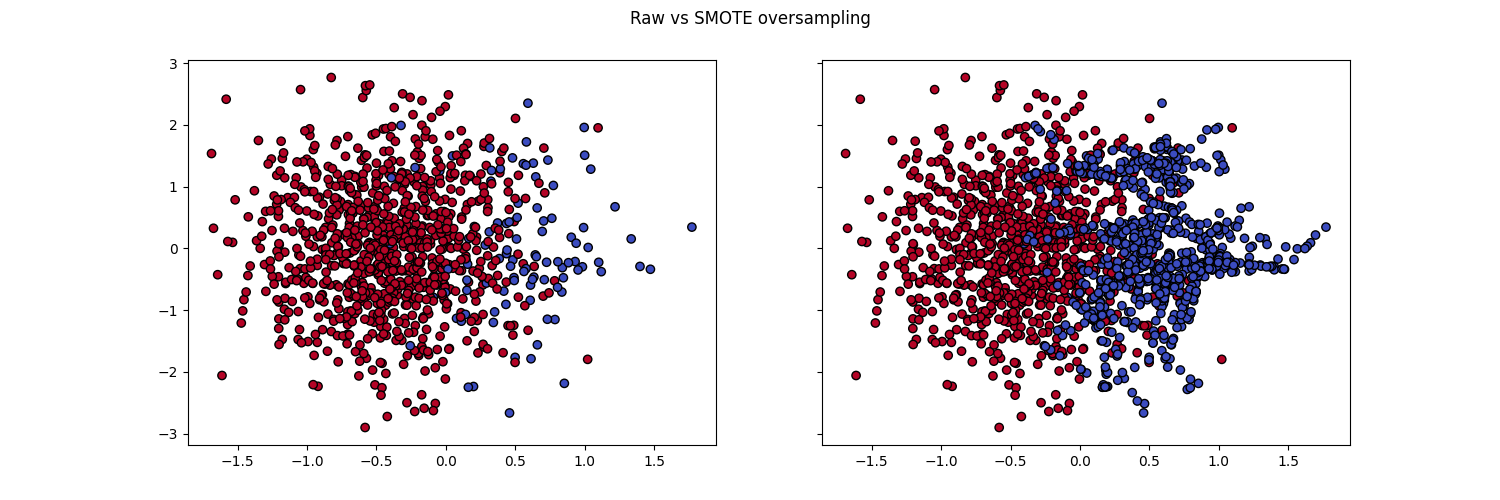
\includegraphics[width=0.8\textwidth]{images/Raw vs SMOTE oversampling.png}
    \caption{SMOTE örneği.}
    \label{fig:enter-label}
\end{figure}

\newpage

\subsection{ADASYN (Adaptive Synthetic Sampling)}
Azınlık sınıfındaki her örneğin etrafındaki hedeflenen komşuluk yoğunluğunu ölçer. Daha az temsil edilen örneklerin etrafında daha fazla sentetik örnek oluşturur. Bu azınlık sınıfındaki daha az temsil edilen bölgelerin daha fazla ağırlığı sahip olmasını sağlar. Sentetik örneklerin daha adaptif bir şekilde oluşturulması, daha az temsil edilen bölgelerde daha fazla vurgu yapılmasına olanak tanır.

\subsubsection{Çalışma Adımları}

\[ r_i = \frac{\text{KNN içindeki çoğunluk sınıfı komşularının sayısı}}{k} \]

Burada, $r_i$ azınlık sınıfına ait $x_i$ gözleminin zorluk derecesini temsil eder.

\[ G_i = r_i \times G \]

Burada, $G_i$ her bir azınlık sınıfı örneği için üretilecek sentetik veri miktarını, $r_i$ azınlık sınıfı örneğinin zorluk derecesini, $G$ toplamda üretilmesi gereken sentetik örnek sayısını temsil eder.

\[ \text{Yeni ornek} = x_i + \lambda \times (x_j - x_i) \]

Burada, $x_i$ azınlık sınıfına ait rastgele bir veri noktasını, $x_j$, $x_i$'nin en yakın komşularından birini, $\lambda$ 0 ile 1 arasında rastgele seçilen bir sayıyı temsil eder.

\begin{enumerate}
    \item İlk adımda, veri kümesindeki azınlık ve çoğunluk sınıfları belirlenir.
    \item ADASYN, her bir azınlık sınıfı gözlemi için çoğunluk sınıfına ait k-en yakın komşuları bulur.
    \item ADASYN, her bir azınlık sınıfı örneğinin zorluk derecesini hesaplar. Zorluk derecesi, bu azınlık örneğinin etrafındaki çoğunluk sınıfı örneklerinin sayısına bağlıdır. Eğer bir azınlık örneği çevresinde çoğunluk sınıfına ait çok fazla komşu varsa, bu örneğin sınıf sınırında olduğu ve sınıflandırılmasının daha zor olduğu anlamına gelir. Zorluk derecesi yüksek olan gözlemler, sınıf sınırında olup sınıflandırılması daha zor olan örneklerdir. ADASYN, bu örneklerin etrafında daha fazla sentetik veri üretmeye odaklanır.
    \item Azınlık sınıfına ait her bir veri noktası için zorluk derecelerini topladıktan sonra, her bir örnek için üretilecek sentetik veri miktarı hesaplar. Zorluk derecesi yüksek olan gözlemlere daha fazla sentetik örnek üretilirken, kolay sınıflandırılabilir gözlemler için daha az sentetik örnek üretilir.
    \item ADASYN, zorluk ağırlıklarına göre sentetik verileri üretir. Bu sentetik örnekler, azınlık sınıfındaki bir veri noktası ile onun en yakın komşuları arasındaki doğrusal interpolasyon kullanılarak üretilir.
\end{enumerate}

\subsubsection{Python Kod Implementasyonu}

\begin{lstlisting}[language=Python]
class ADASYN:
    def __init__(self, k_neighbors=3):
        self.k_neighbors = k_neighbors

    def fit_resample(self, X, y):
        class_counts = Counter(y)
        majority_class_count = max(class_counts.values())

        X_resampled = X
        y_resampled = y

        for class_label, count in class_counts.items():
            if count < majority_class_count:
                n_to_generate = majority_class_count - count
                X_class = X[y == class_label]

                nn = NearestNeighbors(n_neighbors=self.k_neighbors).fit(X_class)
                neighbors = nn.kneighbors(X_class, return_distance=False)

                synthetic_samples = np.zeros((n_to_generate, X.shape[1]))

                for i in range(n_to_generate):
                    sample_idx = np.random.randint(0, X_class.shape[0])
                    neighbor_idx = np.random.choice(neighbors[sample_idx][1:])

                    sample = X_class[sample_idx]
                    neighbor = X_class[neighbor_idx]

                    diff = neighbor - sample
                    gap = np.random.rand()
                    synthetic_samples[i] = sample + gap * diff

                X_resampled = np.vstack((X_resampled, synthetic_samples))
                y_resampled = np.hstack((y_resampled, np.full(n_to_generate, class_label)))

        return X_resampled, y_resampled
\end{lstlisting}

\newpage

\begin{figure}[h]
    \centering
    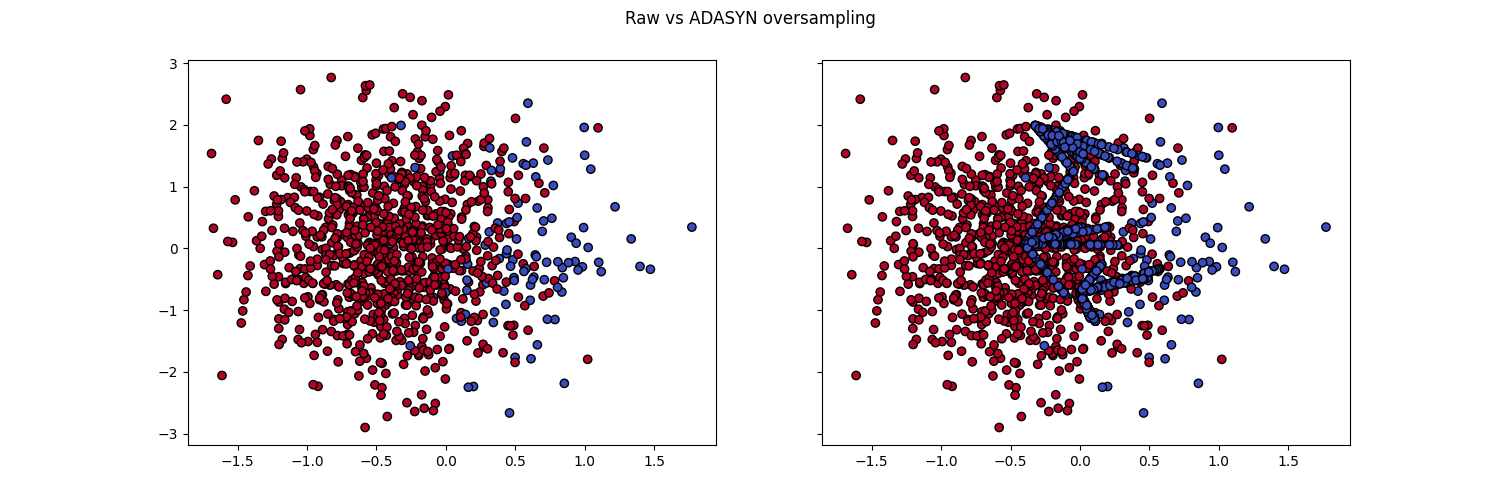
\includegraphics[width=1\textwidth]{images/Raw vs ADASYN oversampling.png}
    \caption{ADASYN örneği.}
    \label{fig:enter-label}
\end{figure}

\newpage

\subsection{Borderline-SMOTE}
Azınlık sınıfındaki örnekler arasında, sınıf sınırlarına yakın olanları belirler. Bu örnekler, genellikle çoğunluk sınıfına daha yakın olup karar sınırlarında yer alan veri noktalarıdır. Sınıf sınırındaki bu örnekler üzerinde sentetik örnekler oluşturarak azınlık sınıfının veri dağılımını artırır. Sentetik örnekler, gerçek verilere benzemesi için bu sınırlardaki veri noktalarının arasında oluşturulur.

\subsubsection{Çalışma Adımları}

\[ \text{Yeni ornek} = x_i + \lambda \times (x_j - x_i) \]

Burada, $x_i$ azınlık sınıfına ait rastgele bir veri noktasını, $x_j$, $x_i$'nin en yakın komşularından birini, $\lambda$ 0 ile 1 arasında rastgele seçilen bir sayıyı temsil eder.

\begin{enumerate}
    \item Öncelikle veri kümesindeki azınlık ve çoğunluk sınıfları belirlenir.
    \item Her bir azınlık sınıfı için k-en yakın komşular algoritması kullanılarak komşular belirlenir. Bu adım, azınlık sınıfı örneklerinin çoğunluk sınıfına ne kadar yakın olduğunu analiz etmek için kullanılır.
    \item Azınlık sınıfındaki her bir örneğin, çoğunluk sınıfı komşularıyla olan etkileşimi değerlendirilir ve bu örnekler üç gruba ayrılır:
    \begin{itemize}
        \item \textbf{Tehlikeli (Borderline) Örnekler}: Çoğunlukla çoğunluk sınıfı ile karışan ve sınıf sınırında bulunan azınlık sınıfı örnekleridir. Bu örnekler, sınıflandırma için kritik öneme sahiptir çünkü bu bölgede doğru bir sınıflandırma yapılmazsa model hatalı sınıflandırmalar yapabilir. Tehlikeli (borderline) örnekler, çoğunluk sınıfına yakın olduklarından dolayı modelin bu bölgedeki sınıf ayrımını güçlendirmek için sentetik veri üretiminin odak noktası olur.
        \item \textbf{Güvenli Örnekler}: Çoğunlukla diğer azınlık sınıfı komşularına sahip, sınıf sınırından uzakta olan güvenli örneklerdir.
        \item \textbf{Gürültü Örnekler}: Azınlık sınıfı olmasına rağmen çoğunluk sınıfı komşuları arasında izole olmuş ve çoğunluk sınıfına yakın yerlerde bulunan örneklerdir. Gürültü örnekler genellikle oversampling sürecine dahil edilmez.
    \end{itemize}
    \item Sadece sınıf sınırında, tehlikeli bölgede bulunan azınlık sınıfı örnekleri için sentetik veri üretimi yapılır. Borderline-SMOTE bu örneklerin en yakın azınlık sınıfı komşularıyla doğrusal interpolasyon yaparak sentetik veri üretir. Ancak, sadece sınıf sınırında bulunan tehlikeli örnekler üzerinden sentetik veri oluşturulur. Bu doğrusal interpolasyon yöntemi, sentetik verilerin, sınıf sınırlarında bulunan azınlık sınıfı örnekleri etrafında üretilmesini sağlar.
\end{enumerate}

\subsubsection{Python Kod Implementasyonu}

\begin{lstlisting}[language=Python]
class BorderlineSMOTE:
    def __init__(self, k_neighbors=5, m_neighbors=10):
        self.k_neighbors = k_neighbors
        self.m_neighbors = m_neighbors

    def fit_resample(self, X, y):
        classes, class_counts = np.unique(y, return_counts=True)
        majority_class = classes[np.argmax(class_counts)]
        minority_class = classes[np.argmin(class_counts)]

        minority_samples = X[y == minority_class]
        majority_samples = X[y == majority_class]

        n_minority_samples = minority_samples.shape[0]
        n_majority_samples = majority_samples.shape[0]
        n_to_generate = n_majority_samples - n_minority_samples

        if n_to_generate <= 0:
            return X, y

        nn_m = NearestNeighbors(n_neighbors=self.m_neighbors).fit(X)
        neighbors_m = nn_m.kneighbors(minority_samples, return_distance=False)

        danger_indices = []
        for i in range(n_minority_samples):
            majority_neighbors = sum(y[neighbors_m[i][1:]] == majority_class)
            if majority_neighbors > (self.m_neighbors / 2):
                danger_indices.append(i)
        
        danger_samples = minority_samples[danger_indices]
        if len(danger_samples) == 0:
            return X, y

        nn_k = NearestNeighbors(n_neighbors=self.k_neighbors).fit(minority_samples)
        neighbors_k = nn_k.kneighbors(danger_samples, return_distance=False)

        synthetic_samples = np.zeros((n_to_generate, X.shape[1]))

        for i in range(n_to_generate):
            sample_idx = np.random.randint(0, len(danger_samples))
            neighbor_idx = np.random.choice(neighbors_k[sample_idx][1:])
            
            sample = danger_samples[sample_idx]
            neighbor = minority_samples[neighbor_idx]
            
            diff = neighbor - sample
            gap = np.random.rand()
            synthetic_samples[i] = sample + gap * diff

        X_resampled = np.vstack((X, synthetic_samples))
        y_resampled = np.hstack((y, np.full(n_to_generate, minority_class)))
        return X_resampled, y_resampled
\end{lstlisting}

\begin{figure}[h]
    \centering
    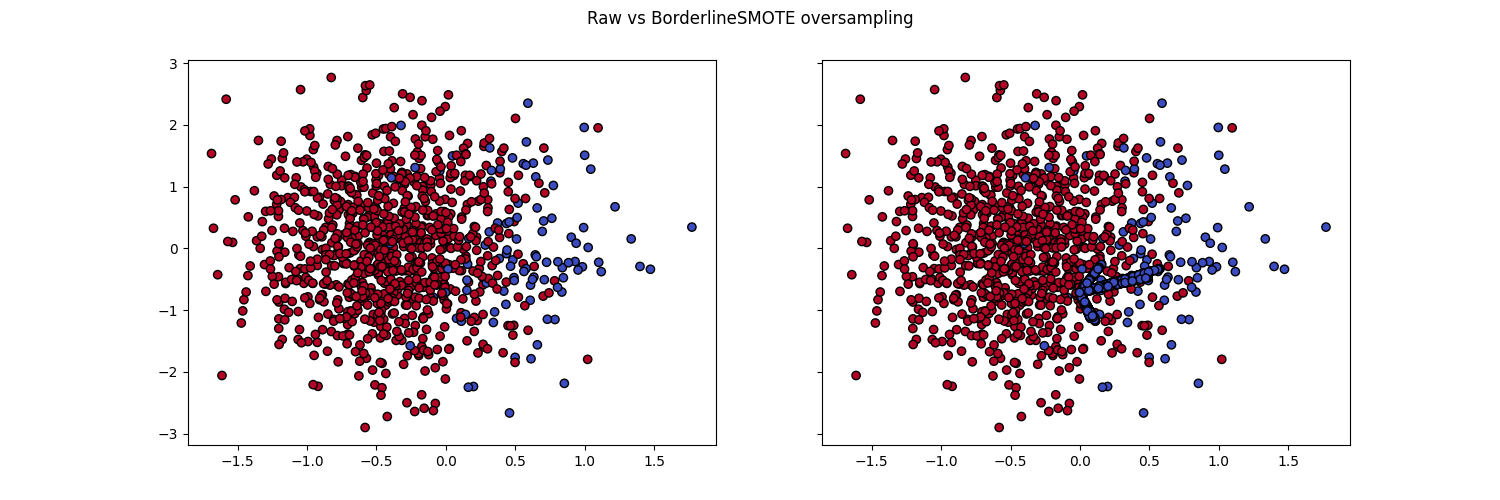
\includegraphics[width=1\textwidth]{images/Raw vs BorderlineSMOTE oversampling.png}
    \caption{Borderline-SMOTE örneği.}
    \label{fig:enter-label}
\end{figure}

\newpage

\subsection{Random Over Sampling}
Azınlık sınıfındaki örneklerin sayısına eşit olacak şekilde, çoğunluk sınıfındaki örnekler rastgele seçilerek artırılır. Bu seçilen örnekler, azınlık sınıfındaki mevcut örneklerle birleştirilerek dengeli bir veri seti oluşturulur. Mevcut veri setini değiştirmez sadece örneklerin tekrarlanmasını kullanır.

\subsubsection{Çalışma Adımları}

\begin{enumerate}
    \item Veri setindeki sınıf dengesizliğini anlamak için önce azınlık ve çoğunluk sınıfları belirlenir.
    \item Çoğunluk sınıfının veri kümesinde kaç gözleme sahip olduğu tespit edilir. Bu adım, azınlık sınıfına ne kadar fazla sentetik örnek ekleneceğini belirler. RandomOverSampler, azınlık sınıfının gözlem sayısını çoğunluk sınıfının gözlem sayısına eşitlemeye çalışır.
    \item Azınlık sınıfı gözlemlerinden rastgele seçim yapılır. RandomOverSampler, azınlık sınıfından rastgele gözlemleri tekrar tekrar seçerek çoğunluk sınıfıyla aynı sayıda gözlem elde edinceye kadar süreci devam ettirir. Seçilen gözlemler mevcut veri setindeki gözlemlerin birebir kopyasıdır; yeni veri noktaları oluşturulmaz, sadece mevcut örnekler çoğaltılır. Bu aşamada rastgele seçim tamamen olasılıksaldır, yani örnekler veri kümesindeki herhangi bir örnekten bağımsız olarak eşit olasılıkla seçilir.
    \item Rastgele seçilen azınlık sınıfı gözlemleri veri setine eklenir. Bu, çoğunluk sınıfının boyutuna kadar devam eder. Her seçilen gözlem, veri setine bir kopyası olarak eklenir, böylece azınlık sınıfının boyutu, çoğunluk sınıfıyla eşit hale gelir.
\end{enumerate}

\subsubsection{Python Kod Implementasyonu}

\begin{lstlisting}[language=Python]
class RandomOverSampler:
    def __init__(self):
        pass

    def fit_resample(self, X, y):
        class_counts = Counter(y)
        max_class_count = max(class_counts.values())

        X_resampled = []
        y_resampled = []

        for class_label, count in class_counts.items():
            X_class = X[y == class_label]

            if count < max_class_count:
                n_to_generate = max_class_count - count
                random_indices = np.random.randint(0, X_class.shape[0], size=n_to_generate)
                X_oversampled = X_class[random_indices]
                X_resampled.append(np.vstack((X_class, X_oversampled)))
                y_resampled.append(np.hstack((np.full(count, class_label), 
                                              np.full(n_to_generate, class_label))))
            else:
                X_resampled.append(X_class)
                y_resampled.append(np.full(X_class.shape[0], class_label))

        X_resampled = np.vstack(X_resampled)
        y_resampled = np.hstack(y_resampled)
        return X_resampled, y_resampled
\end{lstlisting}

\begin{figure}[h]
    \centering
    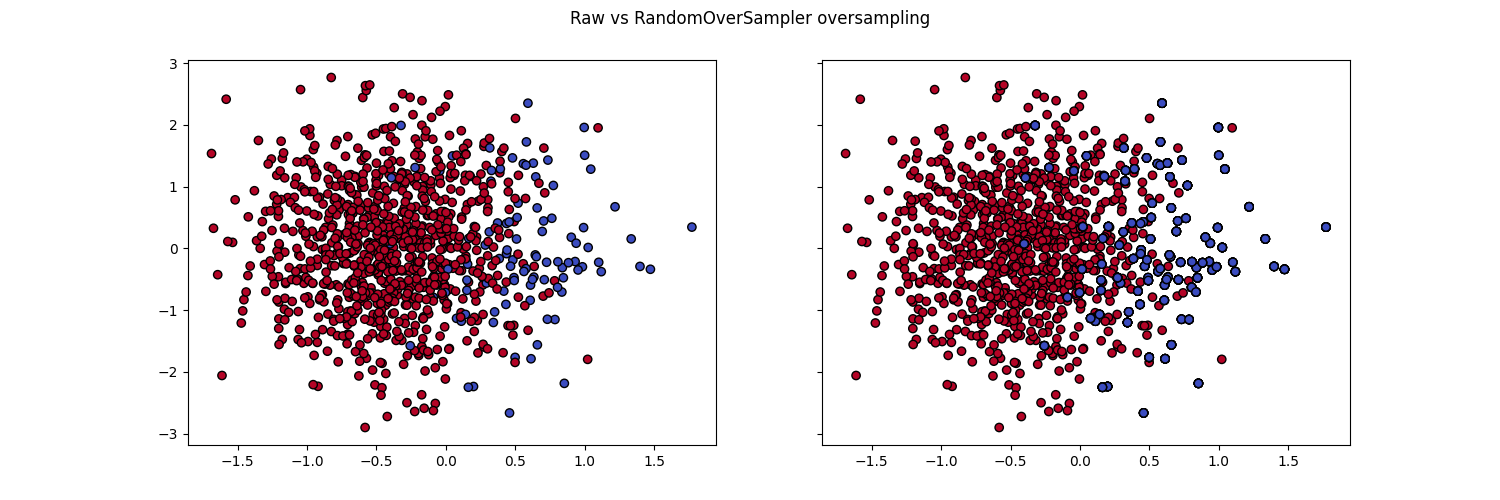
\includegraphics[width=1\textwidth]{images/Raw vs RandomOverSampler oversampling.png}
    \caption{RandomOverSampler örneği.}
    \label{fig:enter-label}
\end{figure}

\newpage

\subsection{Cluster Centroids}
Azınlık sınıfındaki veri noktalarının küme merkezlerini hesaplar. Bu küme merkezleri, çoğunluk sınıfındaki veri noktalarıyla değiştirilir. Bu, azınlık sınıfını temsil etmek için yeni bir alt örneklem oluşturur.

\subsubsection{Çalışma Adımları}

\begin{enumerate}
    \item Veri setindeki sınıf dağılımı incelenir ve azınlık ve çoğunluk sınıfları belirlenir.
    \item ClusterCentroids yönteminin temelinde, çoğunluk sınıfındaki gözlemlerin merkezlerini (centroid) bulmak için k-means kümeleme algoritması kullanılır. K-means, veri kümesini k adet kümeye ayırarak her küme için bir merkez belirler. ClusterCentroids, bu merkez noktalarını seçerek çoğunluk sınıfını azaltır. Bu aşamada, çoğunluk sınıfındaki gözlemler birkaç küme (cluster) oluşturacak şekilde gruplanır ve her küme için bir centroid (merkez noktası) hesaplanır. Bu centroid, küme içindeki tüm gözlemlerin ortalama pozisyonunu temsil eder. K-means algoritması, kümeleri oluştururken her gözlemi en yakın merkeze atar ve bu şekilde kümeleri optimize eder.
    \item K-means algoritması tarafından çoğunluk sınıfındaki gözlemler için oluşturulan her bir kümenin merkezi (centroid), çoğunluk sınıfını temsil eden yeni gözlem olarak seçilir. Bu merkez noktaları, her kümenin genelleştirilmiş bir özetidir ve çoğunluk sınıfındaki gözlemleri daha dengeli ve temsili bir şekilde azaltır. Bu merkezler, çoğunluk sınıfının veri setindeki genel dağılımını en iyi şekilde temsil etmeyi hedefler. Seçilen bu centroidler, çoğunluk sınıfının sayısını düşürerek azınlık sınıfıyla dengelenmesini sağlar.
    \item Centroidler belirlendikten sonra, veri setindeki çoğunluk sınıfı gözlemleri bu merkezlerle değiştirilir. Yani çoğunluk sınıfındaki orijinal gözlemler veri setinden çıkarılır ve yerlerine bu merkezler eklenir. Bu sayede çoğunluk sınıfının sayısı azaltılarak azınlık sınıfı ile dengelenir.
\end{enumerate}

\subsubsection{Python Kod Implementasyonu}

\begin{lstlisting}[language=Python]
class ClusterCentroids:
    def __init__(self, n_clusters=None):
        self.n_clusters = n_clusters

    def fit_resample(self, X, y):
        class_counts = Counter(y)
        minority_class_count = min(class_counts.values())

        X_resampled = []
        y_resampled = []

        for class_label, count in class_counts.items():
            X_class = X[y == class_label]

            if count > minority_class_count:
                kmeans = KMeans(n_clusters=minority_class_count)
                kmeans.fit(X_class)
                centroids = kmeans.cluster_centers_
                X_resampled.append(centroids)
                y_resampled.append(np.full(minority_class_count, class_label))
            else:
                X_resampled.append(X_class)
                y_resampled.append(np.full(X_class.shape[0], class_label))

        X_resampled = np.vstack(X_resampled)
        y_resampled = np.hstack(y_resampled)
        return X_resampled, y_resampled
\end{lstlisting}

\begin{figure}[h]
    \centering
    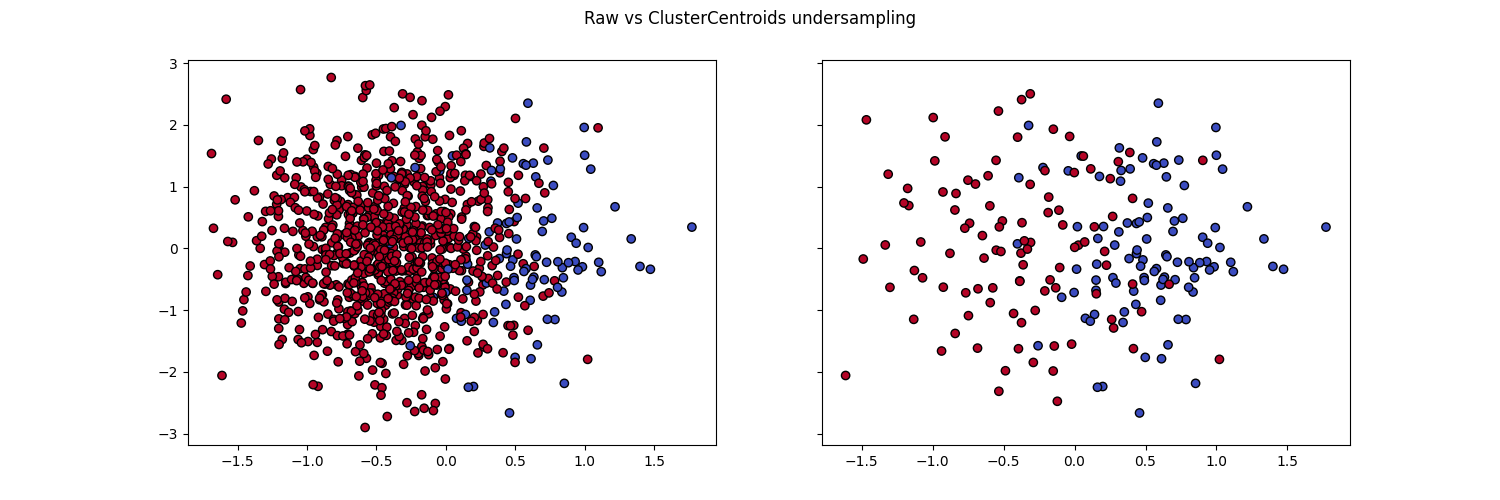
\includegraphics[width=1\textwidth]{images/Raw vs ClusterCentroids undersampling.png}
    \caption{ClusterCentroids örneği.}
    \label{fig:enter-label}
\end{figure}

\newpage

\subsection{Random Under Sampling}
Çoğunluk sınıfından rastgele örnekler seçerek, azınlık sınıfındaki örnek sayısıyla aynı sayıya düşürür. Bu seçilen örnekler, çoğunluk sınıfındaki veri sayısını azaltarak daha dengeli bir veri seti oluşturur.

\subsubsection{Çalışma Adımları}

\begin{enumerate}
    \item İlk adımda, veri setindeki her sınıfın gözlem sayıları hesaplanır ve hangi sınıfın azınlık (minority), hangi sınıfın çoğunluk (majority) sınıf olduğu belirlenir.
    \item RandomUnderSampler, çoğunluk sınıfındaki gözlemlerden rastgele örnekler seçer. Bu rastgele seçilen örnekler, veri setinden çıkarılarak çoğunluk sınıfının boyutunu azaltır. Burada dikkat edilmesi gereken nokta, azınlık sınıfına dokunulmaması ve yalnızca çoğunluk sınıfındaki gözlemlerin azaltılmasıdır.
    \item RandomUnderSampler yönteminde, veri bilimci çoğunluk ve azınlık sınıflarının nasıl dengeleneceğine karar verebilir. Bu dengeleme, "sampling\_strategy" adı verilen bir parametre ile kontrol edilir. Eğer "sampling\_strategy" parametresi belirtilmezse, varsayılan olarak çoğunluk sınıfı azınlık sınıfıyla eşitlenir. Bu parametre ile aşağıdaki senaryolardan biri seçilebilir:
    \begin{itemize}
        \item \textbf{Azınlık sınıfına eşitleme}: Çoğunluk sınıfı, azınlık sınıfıyla aynı sayıya indirgenir. Bu, en yaygın kullanılan stratejidir ve sınıf dengesizliğini tamamen giderir.
        \item \textbf{Belirli bir oran}: Çoğunluk sınıfını, azınlık sınıfından daha büyük ama belirli bir oranla daha küçük hale getirmek mümkündür. Örneğin, çoğunluk sınıfının azınlık sınıfının iki katı kadar olmasını sağlayabilirsiniz.
    \end{itemize}
\end{enumerate}

\subsubsection{Python Kod Implementasyonu}

\begin{lstlisting}[language=Python]
class RandomUnderSampler:
    def __init__(self):
        pass

    def fit_resample(self, X, y):
        classes, class_counts = np.unique(y, return_counts=True)

        min_class_size = np.min(class_counts)

        X_resampled = []
        y_resampled = []

        for class_label in classes:
            class_samples = X[y == class_label]
            n_class_samples = class_samples.shape[0]

            if n_class_samples > min_class_size:
                selected_indices = np.random.choice(class_samples.shape[0], 
                                                    min_class_size, replace=False)
                selected_samples_resampled = class_samples[selected_indices]
            else:
                selected_samples_resampled = class_samples
            
            X_resampled.append(selected_samples_resampled)
            y_resampled.append(np.full(min_class_size, class_label))
            
        X_resampled = np.vstack(X_resampled)
        y_resampled = np.hstack(y_resampled)
        return X_resampled, y_resampled
\end{lstlisting}

\begin{figure}[h]
    \centering
    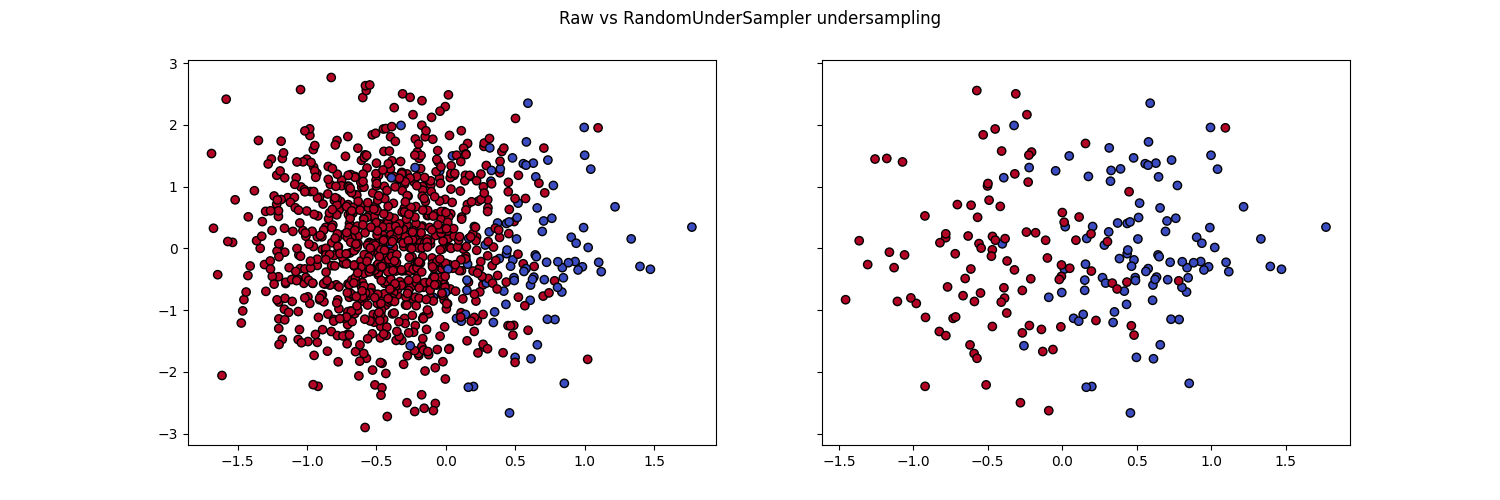
\includegraphics[width=1\textwidth]{images/Raw vs RandomUnderSampler undersampling.png}
    \caption{RandomUnderSampler örneği.}
    \label{fig:enter-label}
\end{figure}

\newpage

\subsection{Near Miss}
Azınlık sınıfına daha yakın olan çoğunluk sınıfı örneklerini belirlemek için bir kriter kullanır. Bu kriter, belirli bir eşik değeri veya uzaklık ölçüsüne dayanır. Seçilen çoğunluk sınıfı örnekleri, azınlık sınıfı ile aralarındaki uzaklık veya farklılık kriterini en iyi şekilde karşılayan örneklerdir. Bu örnekler seçilerek alt örnekleme işlemi gerçekleştirilir.

\subsubsection{Çalışma Adımları}

\begin{enumerate}
    \item İlk adım olarak, veri setinde hangi sınıfın azınlık (minority) ve hangi sınıfın çoğunluk (majority) olduğuna karar verilir.
    \item NearMiss yöntemi, gözlemler arasındaki mesafeleri kullanarak çoğunluk sınıfından seçilecek örnekleri belirler.
    \item NearMiss yönteminin üç farklı versiyonu vardır: NearMiss-1, NearMiss-2, ve NearMiss-3. Bu üç yaklaşım da farklı stratejilerle çoğunluk sınıfından örnek seçimi yapar. Her biri, azınlık sınıfı etrafındaki çoğunluk sınıfı gözlemlerini seçerek, sınıf sınırlarını daha net hale getirmeye çalışır.
    \begin{itemize}
        \item \textbf{NearMiss-1}: Azınlık sınıfındaki her bir gözlem için, ona en yakın olan belirli sayıda çoğunluk sınıfı gözlemini seçer. Yani, azınlık sınıfındaki her gözleme en yakın çoğunluk sınıfı gözlemleri belirlenir ve sadece bu gözlemler veri setinde tutulur. Azınlık sınıfındaki her örnek için çoğunluk sınıfındaki gözlemlerle olan mesafeler hesaplanır. En küçük mesafeye sahip k tane çoğunluk sınıfı gözlemi seçilir. Seçilen çoğunluk sınıfı örnekleri korunur, diğerleri çıkarılır.
        \item \textbf{NearMiss-2}: Her bir çoğunluk sınıfı gözlemi, en uzak azınlık sınıfı gözlemlerine göre seçilir. Bu sayede, çoğunluk sınıfındaki gözlemler arasındaki çeşitlilik artar. Çoğunluk sınıfındaki her örnek için, azınlık sınıfı gözlemleriyle olan mesafeler hesaplanır. Çoğunluk sınıfı gözlemleri arasından, azınlık sınıfına en uzak olan k tane çoğunluk sınıfı gözlemi seçilir ve veri setinde tutulur. Diğer çoğunluk sınıfı gözlemleri çıkarılır.
        \item \textbf{NearMiss-3}: NearMiss-1 ve NearMiss-2'nin bir kombinasyonudur. Bu yöntem, her azınlık sınıfı gözlemi için en yakın çoğunluk sınıfı gözlemlerini seçmek yerine, her çoğunluk sınıfı gözlemi için en yakın azınlık sınıfı gözlemlerini kullanır. Böylece her çoğunluk sınıfı örneği, en yakın azınlık sınıfı gözlemleriyle temsil edilir. Çoğunluk sınıfındaki her gözlem için, en yakın k tane azınlık sınıfı gözlemi belirlenir. Çoğunluk sınıfından en yakın azınlık sınıfına sahip gözlemler veri setinde tutulur. Diğer çoğunluk sınıfı gözlemleri çıkarılır.
    \end{itemize}
    \item NearMiss algoritmasının varyasyonlarından birinin uygulanması sonucunda, veri setinde azınlık ve çoğunluk sınıflarındaki gözlem sayıları daha dengeli hale getirilir
\end{enumerate}

\subsubsection{Python Kod Implementasyonu}

\begin{lstlisting}[language=Python]
class NearMiss:
    def __init__(self, n_neighbors=3):
        self.n_neighbors = n_neighbors

    def fit_resample(self, X, y):
        classes, class_counts = np.unique(y, return_counts=True)
        
        min_class_size = np.min(class_counts)
        
        X_resampled = []
        y_resampled = []
        
        for class_label in classes:
            class_samples = X[y == class_label]
            n_class_samples = class_samples.shape[0]
            
            if n_class_samples > min_class_size:
                nn = NearestNeighbors(n_neighbors=self.n_neighbors)
                nn.fit(class_samples)
                
                distances, _ = nn.kneighbors(class_samples)
                
                sorted_idx = np.argsort(distances.mean(axis=1))
                
                selected_samples = class_samples[sorted_idx[:min_class_size]]
            else:
                selected_samples = class_samples
            
            X_resampled.append(selected_samples)
            y_resampled.append(np.full(min_class_size, class_label))
        
        X_resampled = np.vstack(X_resampled)
        y_resampled = np.hstack(y_resampled)
        return X_resampled, y_resampled
\end{lstlisting}

\newpage

\begin{figure}[h]
    \centering
    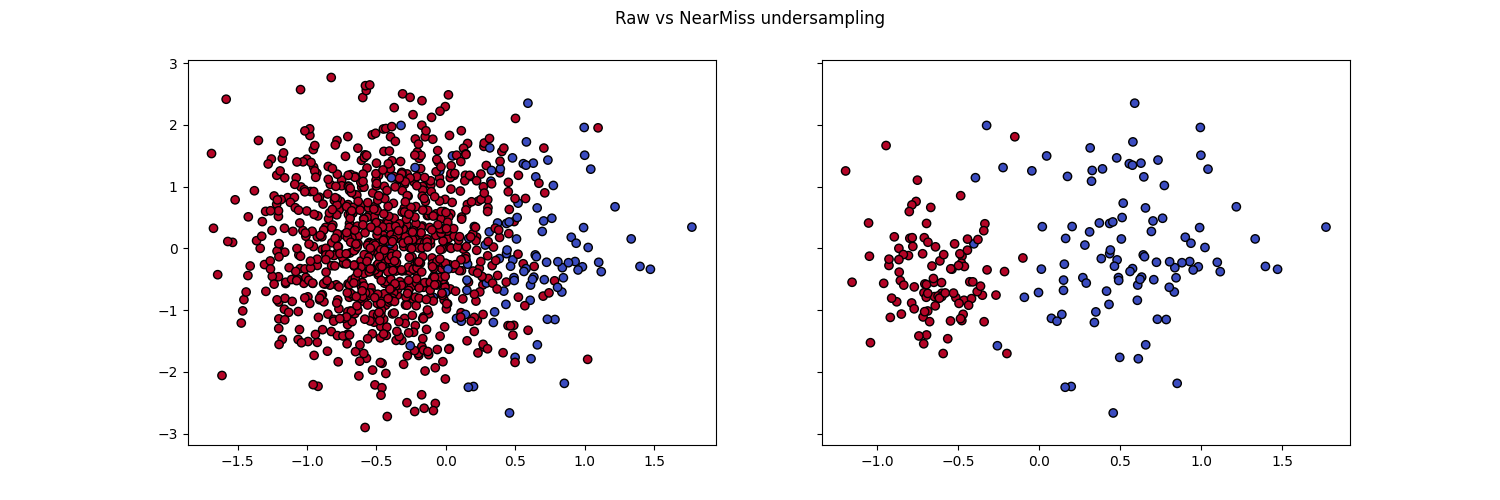
\includegraphics[width=0.8\textwidth]{images/Raw vs NearMiss undersampling.png}
    \caption{NearMiss örneği.}
    \label{fig:enter-label}
\end{figure}

\newpage

\subsection{Tomek Links}
Veri setindeki her bir veri noktası için o veri noktasına en yakın komşusunu bulur. Eğer iki veri noktası birbirlerinin en yakın komşusuysa ve aynı sınıfa ait değillerse, bu iki veri noktası arasındaki ilişkiyi (tomek link) belirler. Bu tomek linke sahip olan veri noktalarından çoğunluk sınıfına ait olan çıkararak veri dengesizliğini azaltır.

\subsubsection{Çalışma Adımları}

\begin{enumerate}
    \item İlk adım olarak, veri setinde hangi sınıfın azınlık (minority) ve hangi sınıfın çoğunluk (majority) olduğuna bakılır.
    \item Tomek Links’in merkezinde, iki farklı sınıfa ait gözlemlerden oluşan komşu çiftlerinin tespiti vardır. Tomek Links algoritması şu adımları izler:
    \begin{itemize}
        \item Tüm veri setindeki örnekler arasında mesafe hesaplanır. Genellikle Euclidean mesafesi kullanılır. Mesafe hesaplandıktan sonra, her örneğin en yakın komşusu bulunur.
        \item Eğer bir örneğin en yakın komşusu, farklı bir sınıfa aitse bu iki örnek bir Tomek Link çifti olarak tanımlanır. Bu durumda, azınlık sınıfına ait bir örneğin en yakın komşusu çoğunluk sınıfına ait olmalıdır ve bu iki örnek birbirine çok yakın mesafede olmalıdır.
        \item Tomek Link çiftleri, genellikle sınıf sınırlarında bulunur. Bu sınırlar, modelin hangi sınıfa ait olduğunu öğrenmekte zorlandığı yerlerdir. Bu nedenle, Tomek Links bu sınırları temizleyerek sınıflar arasındaki farkı daha net hale getirmeyi amaçlar.
    \end{itemize}
    \item Tomek Link çiftleri belirlendikten sonra, çoğunluk sınıfına ait gözlemler bu çiftlerden çıkarılır. Bunun nedeni, bu gözlemlerin sınıf sınırlarında yer alarak modelin öğrenme sürecinde karışıklık yaratmasıdır. Tomek Links, yalnızca çoğunluk sınıfına ait olan gözlemleri kaldırarak azınlık sınıfı örneklerine dokunmaz. Böylece, veri setindeki azınlık sınıfının korunması sağlanır.
\end{enumerate}

\subsubsection{Python Kod Implementasyonu}

\begin{lstlisting}[language=Python]
class TomekLinks:
    def __init__(self):
        pass

    def fit_resample(self, X, y):
        nn = NearestNeighbors(n_neighbors=2)
        nn.fit(X)
        
        distances, indices = nn.kneighbors(X)
        
        tomek_links = []
        
        for i in range(len(X)):
            neighbor_idx = indices[i][1]
            
            if y[i] != y[neighbor_idx]:
                tomek_links.append((i, neighbor_idx))
        
        indices_to_remove = set()
        for i, j in tomek_links:
            if y[i] > y[j]:
                indices_to_remove.add(i)
            else:
                indices_to_remove.add(j)
        
        mask = np.ones(len(X), dtype=bool)
        mask[list(indices_to_remove)] = False
        
        X_resampled = X[mask]
        y_resampled = y[mask]

        class_counts = Counter(y_resampled)
        min_class_count = min(class_counts.values())

        X_balanced = []
        y_balanced = []

        for class_label in class_counts.keys():
            class_indices = np.where(y == class_label)[0]
            selected_indices = np.random.choice(class_indices, 
                                                min_class_count, 
                                                replace=False)
            X_balanced.append(X[selected_indices])
            y_balanced.append(y[selected_indices])

        X_balanced = np.vstack(X_balanced)
        y_balanced = np.hstack(y_balanced)
        
        return X_balanced, y_balanced
\end{lstlisting}

\newpage

\begin{figure}[h]
    \centering
    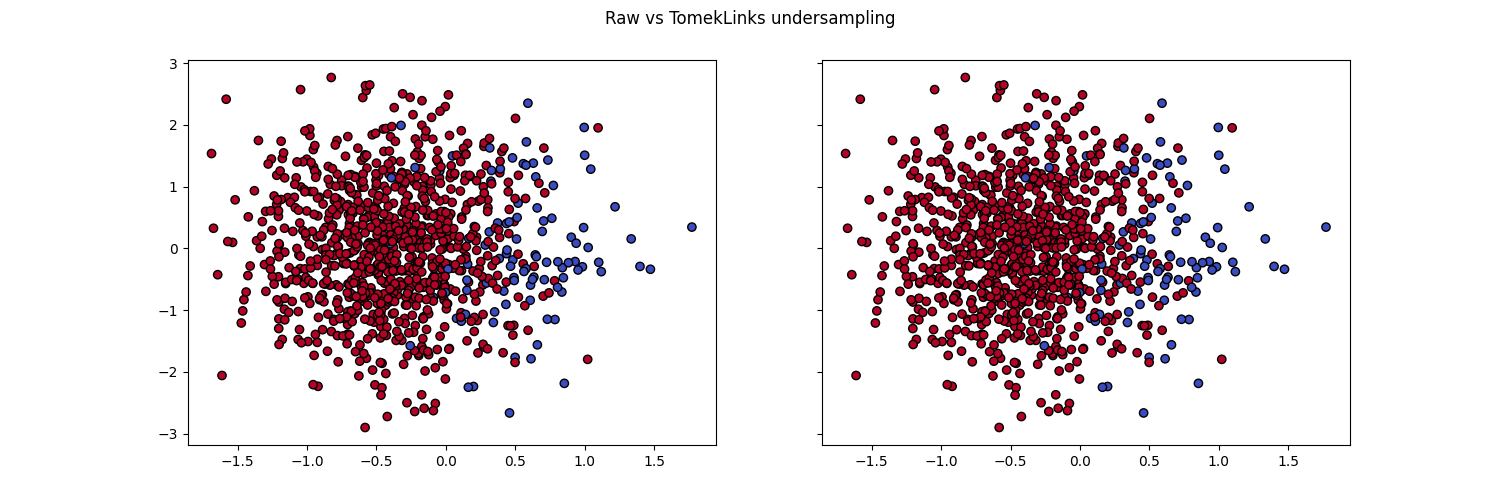
\includegraphics[width=0.8\textwidth]{images/Raw vs TomekLinks undersampling.png}
    \caption{TomekLinks örneği.}
    \label{fig:enter-label}
\end{figure}

\newpage

\subsection{Condensed Nearest Neighbour}
Veri setindeki bir örnek seçilir. Seçilen bu örnek aynı sınıfa ait komşuları ile karşılaştırılır. Eğer bu örnek, aynı sınıfa ait komşularından farklı bir sınıfa aitse, bu örnek korunur ve yeni alt örnekleme setine eklenir. Diğer tüm örnekler bu kriterlere göre kontrol edilir ve veri setinden aynı bilgiyi koruyarak daha küçük bir alt örnekleme seti oluşturulur.

\subsubsection{Çalışma Adımları}

\begin{enumerate}
    \item İlk olarak veri setini iki sınıfa ayırır: azınlık ve çoğunluk sınıfı.
    \item CNN algoritması, azınlık sınıfı gözlemlerinin tamamını ve çoğunluk sınıfından rastgele seçilen bir veya birkaç örneği alarak bir başlangıç kümesi oluşturur. Bu küme, daha sonra büyütülerek çoğunluk sınıfındaki diğer örnekleri temsil edecek şekilde genişletilir.
    \item Başlangıç kümesi oluşturulduktan sonra, kalan çoğunluk sınıfı gözlemleri, başlangıç kümesine eklenip eklenmeyeceğine karar vermek için en yakın komşu (nearest neighbor) sınıflandırmasına tabi tutulur. 
    \begin{itemize}
        \item Kalan çoğunluk sınıfındaki her bir gözlem için, başlangıç kümesindeki gözlemlere olan mesafeler hesaplanır. 
        \item Eğer çoğunluk sınıfındaki bir gözlem, başlangıç kümesine yanlış sınıflandırılmışsa (yani, yanlış sınıf ile tahmin edilmişse), bu gözlem başlangıç kümesine eklenir. 
        \item Eğer çoğunluk sınıfındaki gözlem doğru sınıflandırılmışsa, bu gözlem veri setinden çıkarılır ve alt örnekleme yapılmış veri setine dahil edilmez.
    \end{itemize}
    \item Başlangıç kümesine, yanlış sınıflandırılan çoğunluk sınıfı gözlemleri eklendikçe, bu küme genişler. Hedef, sınıf sınırlarını doğru bir şekilde temsil edebilen bir veri kümesi oluşturmaktır. Bu süreç, tüm gözlemler doğru sınıflanana kadar devam eder. Her iterasyonda, doğru sınıflandırılamayan yeni çoğunluk sınıfı örnekleri kümeye eklenir. Küme genişledikçe, daha az sayıda gözlem eklenmeye başlar çünkü çoğu örnek doğru sınıflandırılır hale gelir. Sonunda, gereksiz gözlemler çıkarılmış olur ve daha küçük bir eğitim veri kümesi elde edilir.
    \item CNN algoritması, tüm çoğunluk sınıfı gözlemleri doğru sınıflandırılana kadar iterasyonlarla devam eder. Bu noktada, eklemeye gerek duyulan yeni gözlem kalmaz ve algoritma durur. Elde edilen alt küme, veri setinin daha kompakt ve daha dengeli bir temsilidir. Algoritma, tüm gözlemler doğru sınıflandırıldığında durur. Alt küme, azınlık sınıfı örnekleri ve doğru sınıflandırılamayan çoğunluk sınıfı örneklerinden oluşur.
\end{enumerate}

\subsubsection{Python Kod Implementasyonu}

\begin{lstlisting}[language=Python]
class CondensedNearestNeighbors:
    def __init__(self, k_neighbors=1):
        self.k_neighbors = k_neighbors

    def fit_resample(self, X, y):
        class_counts = Counter(y)
        min_class_size = min(class_counts.values())
        classes = np.unique(y)

        X_resampled = []
        y_resampled = []

        for class_label in classes:
            X_class = X[y == class_label]
            y_class = y[y == class_label]

            idx_selected = [0]
            knn = KNeighborsClassifier(n_neighbors=self.k_neighbors)

            while len(idx_selected) < min_class_size:
                X_selected = X_class[idx_selected]
                y_selected = y_class[idx_selected]

                knn.fit(X_selected, y_selected)

                for i in range(len(X_class)):
                    if i not in idx_selected:
                        y_pred = knn.predict([X_class[i]])
                        if y_pred != y_class[i]:
                            idx_selected.append(i)

                if len(idx_selected) > min_class_size:
                    idx_selected = np.random.choice(idx_selected, 
                                                    min_class_size,
                                                    replace=False)

            X_resampled.append(X_class[idx_selected])
            y_resampled.append(y_class[idx_selected])

        X_resampled = np.vstack(X_resampled)
        y_resampled = np.hstack(y_resampled)
        return X_resampled, y_resampled
\end{lstlisting}

\newpage

\begin{figure}[h]
    \centering
    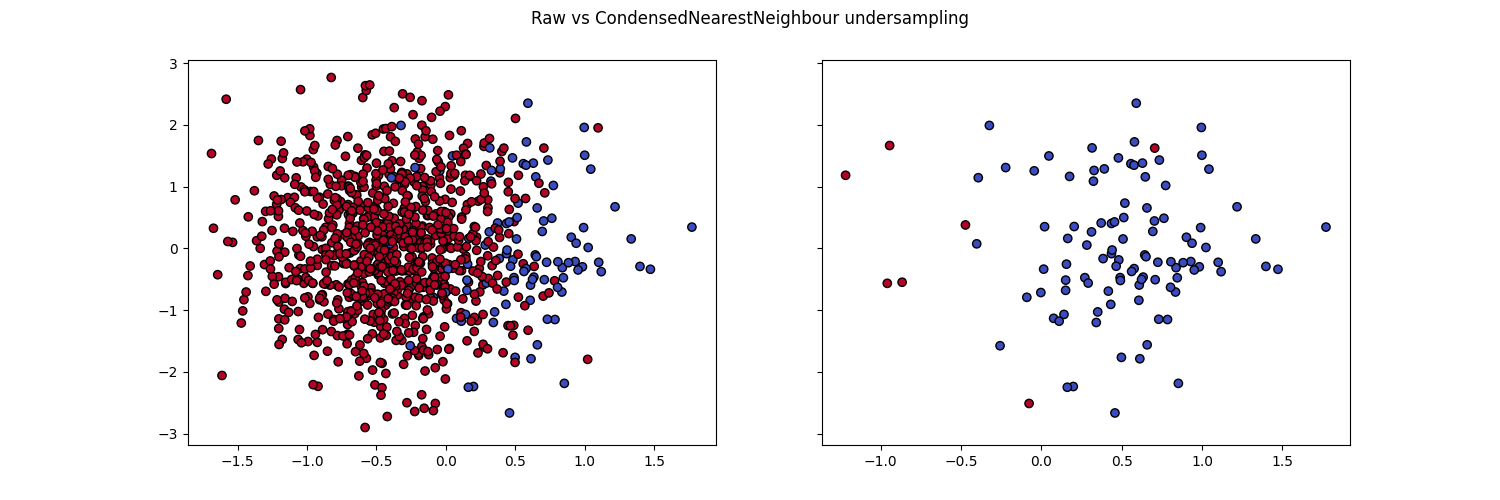
\includegraphics[width=0.8\textwidth]{images/Raw vs CondensedNearestNeighbour undersampling.png}
    \caption{CondensedNearestNeighbour örneği.}
    \label{fig:enter-label}
\end{figure}

\newpage

\subsection{One Sided Selection}
Azınlık sınıfından rastgele bir örnek seçilir. Seçilen bu örnek, çoğunluk sınıfındaki komşuları ile karşılaştırılır. Eğer bu örnek, çoğunluk sınıfındaki örneklerin etkileşimli olduğu bir bölgede bulunmuyorsa ve azınlık sınıfına aitse, bu örnek korunur ve yeni alt örnekleme setine eklenir. Diğer azınlık sınıfı örnekleri de bu şekilde kontrol edilir ve belirli bir kriteri sağlayan örnekler korunarak daha dengeli bir alt örnekleme seti oluşturulur.

\subsubsection{Çalışma Adımları}

\begin{enumerate}
    \item Öncelikle veri seti çoğunluk ve azınlık sınıfı gözlemlerine ayrılır.
    \item Veri setindeki tüm azınlık sınıfı örnekleri başlangıç kümesine eklenir. Çoğunluk sınıfı örnekleri OSS algoritması ile incelenmeye başlanır.
    \item İlk adımda, veri setindeki gürültülü ve yanlış sınıflandırılabilecek çoğunluk sınıfı örnekleri belirlenir ve veri setinden çıkarılır. Bunun için k-en yakın komşu (k-NN) algoritması kullanılır. Çoğunluk sınıfındaki örnekler, k-NN ile tekrar tekrar sınıflandırılır ve yanlış sınıflandırılanlar gürültü olarak kabul edilip kaldırılır.
    \item Gürültü temizlendikten sonra, Tomek Links yöntemi kullanılarak sınırda yer alan gözlemler temizlenir. Tomek Links, iki farklı sınıfa ait örneklerin birbirine en yakın komşular olduğu çiftlerdir. Bu gözlemler sınırda yer aldıkları için, sınıflandırmayı zorlaştırabilir. OSS, bu çiftleri bulur ve çoğunluk sınıfındaki gözlemleri temizler.
    \item Noise Removal ve Tomek Links adımlarından sonra, veri setindeki gereksiz veya yanlış sınıflandırılabilir çoğunluk sınıfı örnekleri kaldırılmış olur. Sonuçta, daha küçük ve daha dengeli bir veri seti elde edilir.
\end{enumerate}

\subsubsection{Python Kod Implementasyonu}

\begin{lstlisting}[language=Python]
class OneSidedSelection:
    def __init__(self, k_neighbors=1):
        self.k_neighbors = k_neighbors

    def fit_resample(self, X, y):
        class_counts = Counter(y)
        minority_class = min(class_counts, key=class_counts.get)
        minority_class_size = class_counts[minority_class]

        X_resampled = []
        y_resampled = []

        for class_label, count in class_counts.items():
            X_class = X[y == class_label]

            if class_label != minority_class:
                knn = KNeighborsClassifier(n_neighbors=self.k_neighbors)
                knn.fit(X_class, np.full(X_class.shape[0], class_label))

                selected_samples = []
                for sample in X_class:
                    neighbors = knn.kneighbors([sample], 
                                        return_distance=False).flatten()
                    if np.all(y[neighbors] == class_label):
                        selected_samples.append(sample)

                selected_samples = np.array(selected_samples)
                if len(selected_samples) > minority_class_size:
                    selected_samples = selected_samples[
                        np.random.choice(len(selected_samples), 
                        minority_class_size, 
                        replace=False)]

                X_resampled.append(selected_samples)
                y_resampled.append(np.full(minority_class_size, class_label))
            else:
                X_resampled.append(X_class)
                y_resampled.append(np.full(X_class.shape[0], class_label))

        X_resampled = np.vstack(X_resampled)
        y_resampled = np.hstack(y_resampled)

        return X_resampled, y_resampled
\end{lstlisting}

\begin{figure}[h]
    \centering
    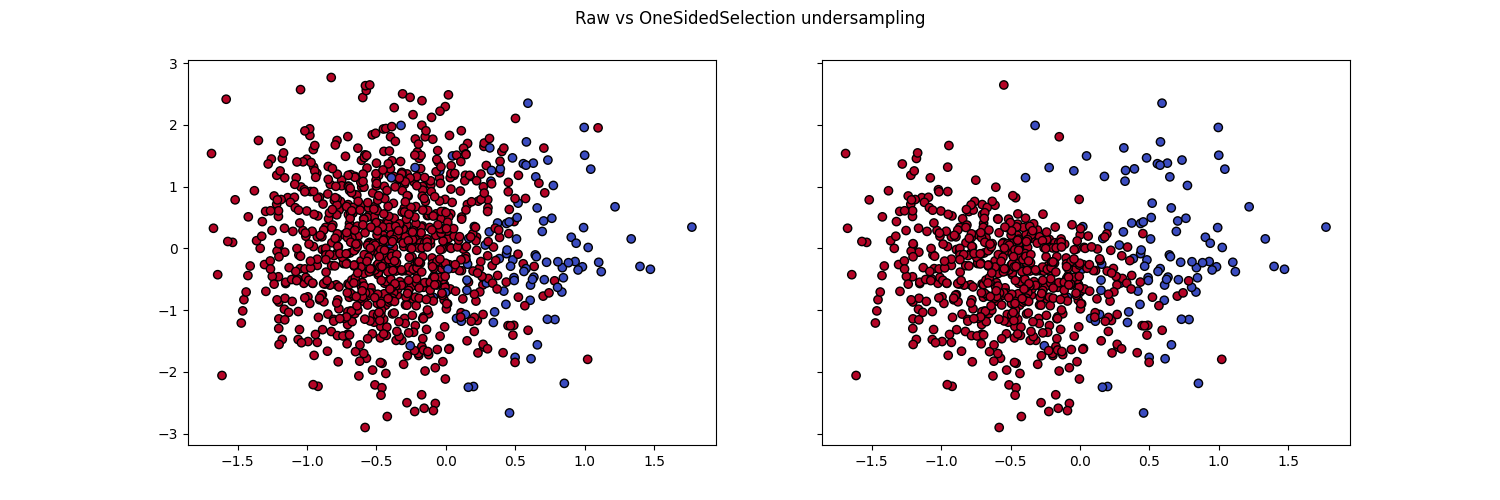
\includegraphics[width=0.8\textwidth]{images/Raw vs OneSidedSelection undersampling.png}
    \caption{OneSidedSelection örneği.}
    \label{fig:enter-label}
\end{figure}

\newpage

\subsection{Neighbourhood Cleaning Rule}
Azınlık sınıfındaki bir örnek seçilir. Seçilen bu örnek, çoğunluk ve azınlık sınıflarının sınırlarındaki bölgelerdeki örnekleri inceler. Eğer bir örnek, kendi sınıfına ait değilse veya farklı bir sınıfa ait komşuları varsa, bu örnek kaldırılır. Diğer örnekler de aynı şekilde incelenerek belirli bir kriteri sağlamayan örnekler kaldırılır ve daha dengeli bir alt örnekleme seti oluşturulur.

\subsubsection{Çalışma Adımları}

\begin{enumerate}
    \item İlk olarak, veri setindeki tüm gözlemler (çoğunluk ve azınlık sınıfı) ayrılır.
    \item Bu adımda, her bir örnek için komşuları değerlendirilir. Burada k-NN (k-En Yakın Komşu) algoritması kullanılarak her veri noktasının k komşusu belirlenir. Amaç, her örneğin komşuları tarafından doğru şekilde sınıflandırılıp sınıflandırılmadığını anlamaktır. Eğer bir örnek, çoğunlukla hatalı bir sınıf ile sınıflandırılmışsa bu örnek, veri setinden çıkarılır.
    \item NCR, azınlık sınıfı gözlemlerini de inceler. Azınlık sınıfındaki bir veri noktası, k komşusu arasında çoğunluk sınıfıyla yanlış sınıflandırılıyorsa, bu azınlık sınıfı örneği de veri setinden çıkarılır. Bu adım, hatalı sınıflandırmaya neden olabilecek sınırda yer alan azınlık sınıfı örneklerini de temizlemeyi amaçlar.
    \item NCR, çoğunluk sınıfındaki gereksiz örnekleri temizlemek için sınıf sınırlarına odaklanır. Tomek Links gibi tekniklerle sınıf sınırındaki gereksiz gözlemler belirlenir ve veri setinden çıkarılır. Özellikle çoğunluk sınıfının gereksiz bir şekilde sınırda yer aldığı durumlar, modelin hatalı sınıflandırmalara yol açabileceği durumlar arasında sayılır.
    \item Yukarıdaki adımlar sonucunda, gereksiz, hatalı veya sınırda yer alan çoğunluk ve azınlık sınıfı örnekleri veri setinden temizlenir. Sonuç olarak, sınıf sınırlarını daha iyi temsil eden ve hatalı sınıflandırma riskini azaltan bir veri seti elde edilir.
\end{enumerate}

\subsubsection{Python Kod Implementasyonu}

\begin{lstlisting}[language=Python]
class NeighbourhoodCleaningRule:
    def __init__(self, k_neighbors=3):
        self.k_neighbors = k_neighbors

    def fit_resample(self, X, y):
        class_counts = Counter(y)
        min_class_size = min(class_counts.values())
        classes = np.unique(y)

        X_resampled = []
        y_resampled = []

        for class_label in classes:
            X_class = X[y == class_label]
            y_class = y[y == class_label]

            knn = KNeighborsClassifier(n_neighbors=self.k_neighbors)
            knn.fit(X, y)

            indices_to_keep = []
            for i in range(len(X_class)):
                neighbors = knn.kneighbors([X_class[i]], return_distance=False)[0]
                y_neighbors = y[neighbors]

                if np.bincount(y_neighbors).argmax() == class_label:
                    indices_to_keep.append(i)

            X_class_cleaned = X_class[indices_to_keep]
            y_class_cleaned = y_class[indices_to_keep]

            if len(X_class_cleaned) > min_class_size:
                indices_to_sample = np.random.choice(len(X_class_cleaned), min_class_size, replace=False)
                X_class_cleaned = X_class_cleaned[indices_to_keep]
                y_class_cleaned = y_class_cleaned[indices_to_keep]

            X_resampled.append(X_class_cleaned)
            y_resampled.append(y_class_cleaned)

        X_resampled = np.vstack(X_resampled)
        y_resampled = np.hstack(y_resampled)
        return X_resampled, y_resampled
\end{lstlisting}

\begin{figure}[h]
    \centering
    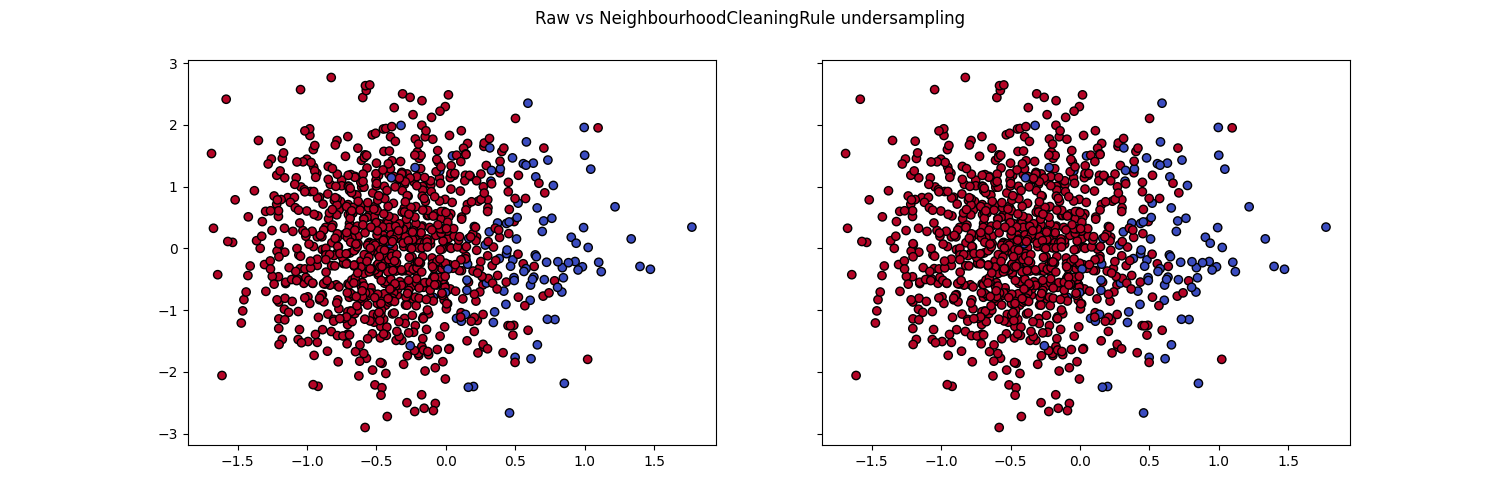
\includegraphics[width=0.6\textwidth]{images/Raw vs NeighbourhoodCleaningRule undersampling.png}
    \caption{NeighbourhoodCleaningRule örneği.}
    \label{fig:enter-label}
\end{figure}

\newpage

\subsection{Edited Nearest Neighbours (ENN)}
Başlangıçta, veri setindeki her bir örneğin sınıf etiketleri kontrol edilir. Her bir örnek için, bu örneğin sınıf etiketi ile k-NN (k en yakın komşu) algoritması kullanılarak belirlenen komşuların sınıf etiketleri karşılaştırılır. Eğer bir örnek, en azından biriyle komşu olmak üzere çoğunluk sınıfı etiketine sahip bir komşusu varsa ve kendisi azınlık sınıfına aitse, bu örnek veri setinden çıkarılır. Diğer örnekler de aynı şekilde incelenerek belirli bir kriteri sağlamayan örnekler kaldırılır ve daha dengeli bir alt örnekleme seti oluşturulur.

\subsubsection{Çalışma Adımları}

\begin{enumerate}
    \item İlk olarak, elimizdeki dengesiz veri seti hazırlanır. Bu veri seti hem çoğunluk sınıfı hem de azınlık sınıfı örneklerini içerir.
    \item ENN, her bir veri noktasının etrafındaki komşuları analiz eder. Bu işlem, k-NN algoritması ile yapılır. Amaç, her bir veri noktasının kendi sınıfında mı yoksa farklı bir sınıfta mı olduğunu anlamaktır.
    \item Her bir veri noktası, komşularıyla olan ilişkisine göre sınıflandırılır. Eğer bir veri noktası, komşularının çoğunluğu tarafından farklı bir sınıfa atanıyorsa, bu noktada bir sınıf karışıklığı yaşandığı kabul edilir.
    \item Eğer bir veri noktası, komşularının çoğu tarafından yanlış sınıflandırılıyorsa (örneğin, çoğunluk sınıfı bir örnek azınlık sınıfı gibi görünüyorsa), bu veri noktası veri setinden çıkarılır. Bu adım, özellikle çoğunluk sınıfı örneklerinin, azınlık sınıfı ile sınıf sınırlarında karışıklık yaratmasını engellemeye yöneliktir.
    \item ENN, yalnızca çoğunluk sınıfı değil, aynı zamanda azınlık sınıfı örnekleri üzerinde de çalışır. Eğer azınlık sınıfına ait bir veri noktası, k komşusunun çoğunluğu tarafından yanlış sınıflandırılıyorsa, bu nokta da veri setinden çıkarılabilir.
    \item Yukarıdaki adımlar sonucunda, yanlış sınıflandırılan veya gereksiz veri noktaları çıkarılarak veri seti yeniden oluşturulur.
\end{enumerate}

\subsubsection{Python Kod Implementasyonu}

\begin{lstlisting}[language=Python]
class EditedNearestNeighbors:
    def __init__(self, k_neighbors=3):
        self.k_neighbors = k_neighbors

    def fit_resample(self, X, y):
        class_counts = Counter(y)
        min_class_size = min(class_counts.values())
        classes = np.unique(y)
        
        X_resampled = []
        y_resampled = []

        for class_label in classes:
            X_class = X[y == class_label]
            
            knn = KNeighborsClassifier(n_neighbors=self.k_neighbors)
            knn.fit(X, y)
            
            neighbors = knn.kneighbors(X_class, return_distance=False)
            to_remove = []
            for i, idx in enumerate(neighbors):
                neighbor_labels = y[idx]
                if np.sum(neighbor_labels == class_label) <= (self.k_neighbors // 2):
                    to_remove.append(i)

            X_cleaned = np.delete(X_class, to_remove, axis=0)
            
            if X_cleaned.shape[0] > min_class_size:
                idx_to_keep = np.random.choice(X_cleaned.shape[0], min_class_size, replace=False)
                X_cleaned = X_cleaned[idx_to_keep]

            X_resampled.append(X_cleaned)
            y_resampled.append(np.full(X_cleaned.shape[0], class_label))

        X_resampled = np.vstack(X_resampled)
        y_resampled = np.hstack(y_resampled)

        return X_resampled, y_resampled
\end{lstlisting}

\begin{figure}[h]
    \centering
    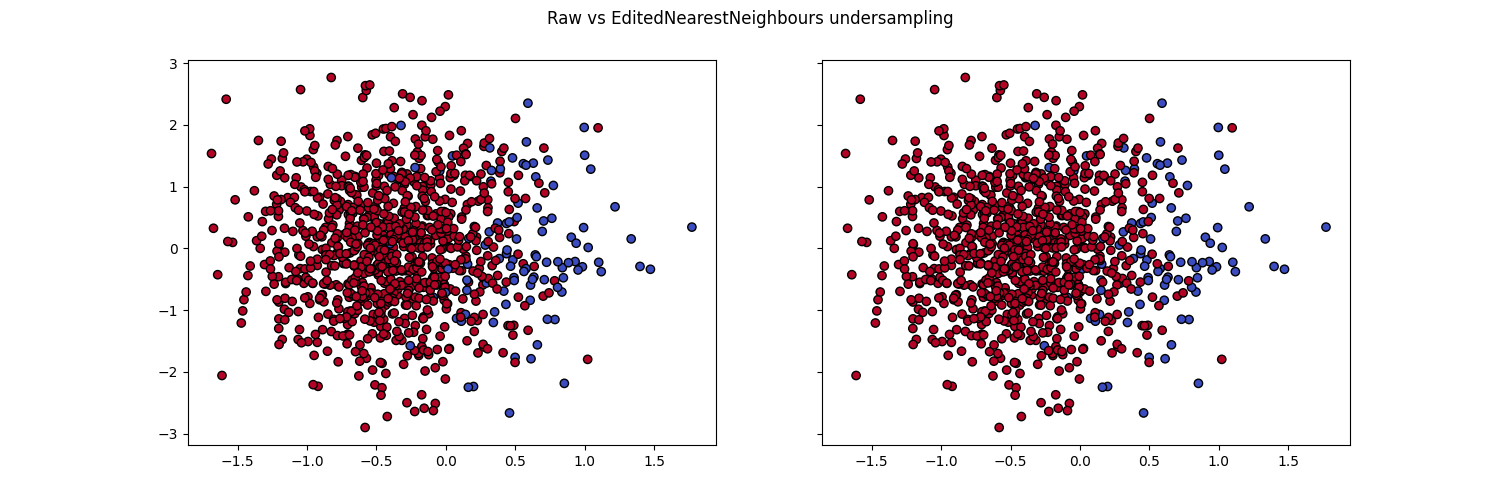
\includegraphics[width=0.6\textwidth]{images/Raw vs EditedNearestNeighbours undersampling.png}
    \caption{EditedNearestNeighbours örneği.}
    \label{fig:enter-label}
\end{figure}

\newpage

\subsection{Repeated Edited Nearest Neighbours (RENN)}
Başlangıçta, veri setindeki her bir örneğin sınıf etiketleri kontrol edilir. Her bir örnek için, bu örneğin sınıf etiketi ile k-NN (k en yakın komşu) algoritması kullanılarak belirlenen komşuların sınıf etiketleri karşılaştırılır. Eğer bir örnek, en azından biriyle komşu olmak üzere çoğunluk sınıfı etiketine sahip bir komşusu varsa ve kendisi azınlık sınıfına aitse, bu örnek veri setinden çıkarılır. Ardışık iterasyonlarla bu işlem tekrarlanarak, alt örnekleme seti güncellenir.

\subsubsection{Çalışma Adımları}

\begin{enumerate}
    \item Öncelikle elimizdeki dengesiz veri seti hazırlanır. Bu veri seti hem çoğunluk sınıfı hem de azınlık sınıfı örneklerini içerir.
    \item İlk adımda her bir veri noktası için en yakın k komşusu belirlenir. 
    \item Her bir veri noktası, komşularıyla karşılaştırılır. Eğer bir veri noktası komşularının çoğunluğu ile aynı sınıfta değilse, bu noktada bir sınıf sınırı karışıklığı olduğu kabul edilir.
    \item Eğer bir veri noktası komşularının çoğunluğu tarafından yanlış sınıflandırılıyorsa (örneğin, çoğunluk sınıfı bir örnek azınlık sınıfına ait gibi görünüyorsa), bu veri noktası veri setinden çıkarılır.
    \item RENN, bu temizleme işlemini yalnızca bir kez yapmaz. İlk temizlikten sonra, elde edilen yeni veri seti tekrar gözden geçirilir. Yeniden oluşturulan veri setinde, her bir veri noktası yeniden komşularıyla karşılaştırılır ve yanlış sınıflandırılan noktalar tekrar temizlenir. Bu süreç, veri setinde artık çıkarılacak veri kalmayana veya bir önceki temizleme adımı ile yeni adım arasında bir fark kalmayana kadar devam eder. Her döngüde yeni yanlış sınıflandırmalar tespit edilirse, bu noktalar çıkarılır. RENN bu tekrarlı temizleme sayesinde, daha temiz ve dengeli bir veri seti oluşturur.
    \item Temizlik işlemi birkaç iterasyondan sonra sona erer. İki ardışık temizleme işlemi arasında veri seti artık değişmediğinde, yani çıkarılacak yeni veri noktası kalmadığında algoritma durur.
\end{enumerate}

\subsubsection{Python Kod Implementasyonu}

\begin{lstlisting}[language=Python]
class RepeatedEditedNearestNeighbors:
    def __init__(self, k_neighbors=3):
        self.k_neighbors = k_neighbors

    def fit_resample(self, X, y):
        class_counts = Counter(y)
        min_class_size = min(class_counts.values())
        classes = np.unique(y)

        X_resampled = []
        y_resampled = []

        for class_label in classes:
            X_class = X[y == class_label]
            y_class = y[y == class_label]

            knn = KNeighborsClassifier(n_neighbors=self.k_neighbors)
            removed = True

            while removed:
                removed = False
                knn.fit(X_class, y_class)

                indices_to_keep = []
                for i in range(len(X_class)):
                    neighbors = knn.kneighbors([X_class[i]], return_distance=False)[0]
                    neighbors = neighbors[neighbors != i]
                    y_neighbors = y_class[neighbors]

                    if np.bincount(y_neighbors).argmax() == y_class[i]:
                        indices_to_keep.append(i)
                    else:
                        removed = True
                        
                X_class = X_class[indices_to_keep]
                y_class = y_class[indices_to_keep]

            if len(X_class) > min_class_size:
                indices_to_sample = np.random.choice(len(X_class), min_class_size, replace=False)
                X_class = X_class[indices_to_sample]
                y_class = y_class[indices_to_sample]

            X_resampled.append(X_class)
            y_resampled.append(y_class)

        X_resampled = np.vstack(X_resampled)
        y_resampled = np.hstack(y_resampled)

        return X_resampled, y_resampled
\end{lstlisting}

\newpage

\begin{figure}[h]
    \centering
    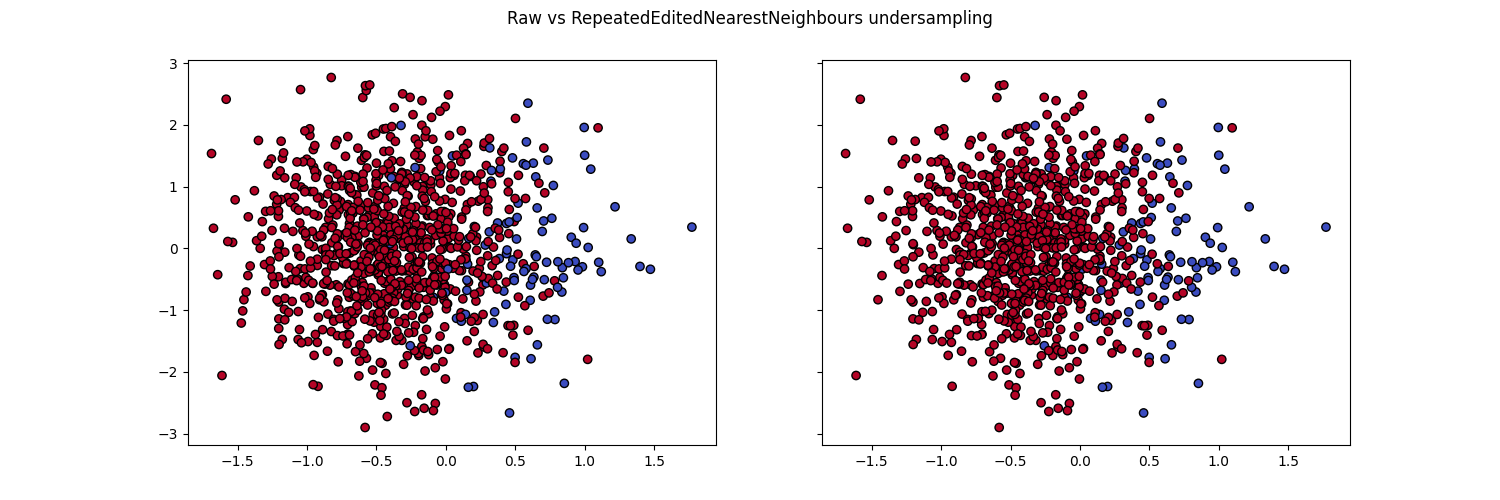
\includegraphics[width=0.6\textwidth]{images/Raw vs RepeatedEditedNearestNeighbours undersampling.png}
    \caption{RepeatedEditedNearestNeighbours örneği.}
    \label{fig:enter-label}
\end{figure}

\newpage

\subsection{AllKNN}
Veri setindeki her bir örnek için, k-NN algoritması kullanılarak örneğin etrafındaki komşular bulunur. Eğer bir örnek, en az k kadar komşusundan çoğunluk sınıfına aitse, bu örnek korunur. Eğer değilse, azınlık sınıfına aitse ve k değerinden az sayıda komşusu çoğunluk sınıfına aitse bu örnek veri setinden çıkarılır. Tüm örnekler bu şekilde kontrol edilerek, sınıf dengesizliği azaltmak için uygun olanlar belirlenir ve veri seti güncellenir.

\subsubsection{Çalışma Adımları}

\begin{enumerate}
    \item Veri setindeki her sınıfın gözlem sayıları hesaplanır ve hangi sınıfın azınlık (minority) ve hangi sınıfın çoğunluk (majority) olduğu belirlenir.
    \item AllKNN, veri setindeki her gözlem için KNN algoritmasını kullanarak bir komşuluk ilişkisi oluşturur. Bu yöntem, her gözlem için en yakın k komşusunu bulur.
    \item AllKNN’in ana amacı, sınıf sınırında veya komşuluk ilişkisine uymayan çoğunluk sınıfına ait örnekleri tespit etmektir. Bu örnekler:
    \begin{itemize}
        \item Eğer bir çoğunluk sınıfına ait örnek, komşularının büyük çoğunluğu azınlık sınıfına aitse, bu örnek sınıf sınırlarında bulunuyor olabilir ve modelin performansını kötü etkileyebilir. Bu tür gözlemler gereksiz olarak işaretlenir.
        \item Çok yakınında farklı sınıflara ait komşuları olan gözlemler, sınıf sınırlarında karışıklık yaratabilir ve bu da modelin tahmin performansını düşürebilir. Bu gözlemler çıkarılır.
    \end{itemize}
    \item KNN algoritmasıyla tespit edilen gereksiz çoğunluk sınıfı gözlemleri, veri setinden çıkarılır. Bu işlem, veri setinin dengesini sağlayarak azınlık sınıfının daha iyi temsil edilmesini sağlar. Veri setindeki gözlemler çıkarılırken gözlemlerin komşularına göre sınıf sınırında yer alıp almadıkları dikkate alınır. Çoğunluk sınıfındaki gözlemlerin sayısı, azınlık sınıfına göre belirli bir seviyeye indirgenir. Ancak azınlık sınıfı gözlemlerine dokunulmaz.
\end{enumerate}

\subsubsection{Python Kod Implementasyonu}

\begin{lstlisting}[language=Python]
class AllKNN:
    def __init__(self, k=3):
        self.k = k

    def fit_resample(self, X, y):
        nn = NearestNeighbors(n_neighbors=self.k + 1)
        nn.fit(X)

        distances, indices = nn.kneighbors(X)

        indices_to_remove = []

        for i in range(len(X)):
            neighbors = indices[i][1:]

            neighbor_labels = y[neighbors]
            if Counter(neighbor_labels).most_common(1)[0][0] != y[i]:
                indices_to_remove.append(i)

        mask = np.ones(len(X), dtype=bool)
        mask[indices_to_remove] = False
        X_resampled = X[mask]
        y_resampled = y[mask]

        class_counts = Counter(y_resampled)
        min_class_count = min(class_counts.values())

        X_balanced = []
        y_balanced = []

        for class_label in class_counts.keys():
            class_indices = np.where(y == class_label)[0]
            selected_indices = np.random.choice(
                class_indices, min_class_count, replace=False)
            X_balanced.append(X[selected_indices])
            y_balanced.append(y[selected_indices])

        X_balanced = np.vstack(X_balanced)
        y_balanced = np.hstack(y_balanced)
        return X_balanced, y_balanced
\end{lstlisting}

\begin{figure}[h]
    \centering
    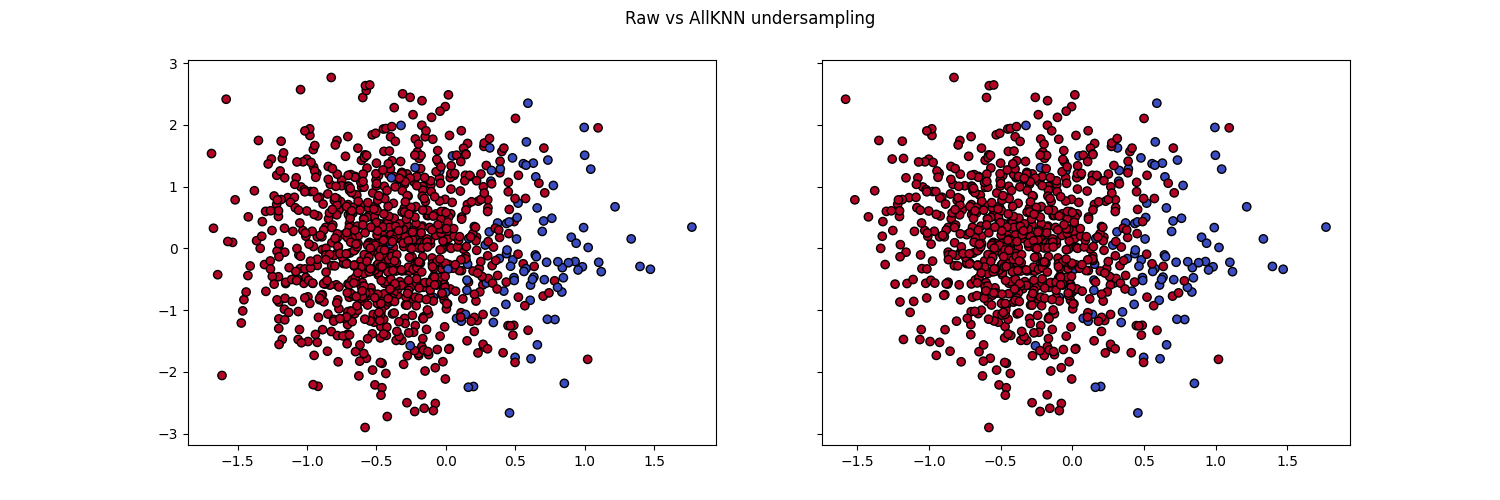
\includegraphics[width=1\textwidth]{images/Raw vs AllKNN undersampling.png}
    \caption{AllKNN örneği.}
    \label{fig:enter-label}
\end{figure}

\newpage

\subsection{Instance Hardness Threshold}
Her bir örnek için, bir sınıflandırma modeli (genellikle k-NN veya bir karar ağacı kullanılır) kullanılarak örneklerin zorluk seviyesi belirlenir. Bu, örneğin yanlış sınıflandırılma olasılığı veya belirsizlik derecesi gibi faktörlere dayanabilir. Bir eşik değeri belirlenir. Bu eşik değeri, seçilecek veya kaldırılacak örneklerin zorluk seviyesini belirler. Örnekler, belirlenen eşik değerine göre değerlendirilir. Eşik değerini geçen örnekler, model için zor olan veya belirsiz olan örnekler olarak kabul edilir ve kaldırılabilir veya azaltılabilir.

\subsubsection{Çalışma Adımları}

\begin{enumerate}
    \item İlk olarak, veri seti azınlık ve çoğunluk sınıflarını içerir.
    \item IHT, örneklerin zorluk seviyelerini belirlemek için bir sınıflandırma modeli kullanır. Genellikle bu amaçla lojistik regresyon, karar ağaçları veya destek vektör makineleri (SVM) gibi modeller tercih edilir. Veri setindeki her örnek için model eğitilir ve tahmin yapılır. Bu model, veri setindeki her bir örnek için hardness score (zorluk puanı) hesaplamak üzere kullanılır. Bu puan, modelin o örneği doğru sınıflandırıp sınıflandıramadığını gösterir.
    \item Zorluk puanı, her veri noktasının sınıflandırma modeline göre ne kadar zor sınıflandırıldığına dair bir ölçüdür. Bir örneğin zorluk puanı, modelin o örneği yanlış sınıflandırma olasılığına dayalıdır. Eğer model bir veri noktasını sınıflandırmakta zorlanıyorsa, o noktaya yüksek bir zorluk puanı atanır. Bu puanlar genellikle 0 ile 1 arasında bir değer alır:
    \begin{itemize}
        \item \textbf{1}: Örnek yanlış sınıflandırılmıştır ve zor bir örnektir.
        \item \textbf{0}: Örnek doğru sınıflandırılmıştır ve kolay bir örnektir.
    \end{itemize}
    \item Zorluk puanları hesaplandıktan sonra, hangi örneklerin veri setinden çıkarılacağına karar vermek için bir eşik değeri (threshold) belirlenir. Bu eşik değeri, zorluk puanı eşikten yüksek olan örneklerin çıkarılmasını sağlar. Eşik değeri ne kadar düşükse, daha fazla örnek çıkarılır. Çoğunluk sınıfından, zorluk puanı belirlenen eşiği aşan örnekler, veri setinden çıkarılır.
    \item Zorluk puanı belirlenen eşiğin üzerinde olan çoğunluk sınıfına ait örnekler, veri setinden çıkarılır. Bu işlem, veri setindeki gürültülü ve yanlış sınıflandırılmış örnekleri temizlemeyi hedefler. Böylece modelin yanlış öğrendiği veriler çıkarılmış olur. Zor örnekler genellikle sınıf sınırlarında yer alan, birbirine çok yakın ya da yanlış etiketlenmiş veriler olabilir.
    \item Çoğunluk sınıfından zor örnekler çıkarıldığında, veri seti daha dengeli hale gelir. Temizlenen veri seti, azınlık sınıfının daha iyi temsil edilmesini sağlar.
\end{enumerate}

\subsubsection{Python Kod Implementasyonu}

\begin{lstlisting}[language=Python]
from imblearn.under_sampling import InstanceHardnessThreshold
from sklearn.linear_model import LogisticRegression

iht = InstanceHardnessThreshold(random_state=0, sampling_strategy="auto", estimator=LogisticRegression())
X_resampled, y_resampled = iht.fit_resample(X_train, y_train)
\end{lstlisting}

\begin{figure}[h]
    \centering
    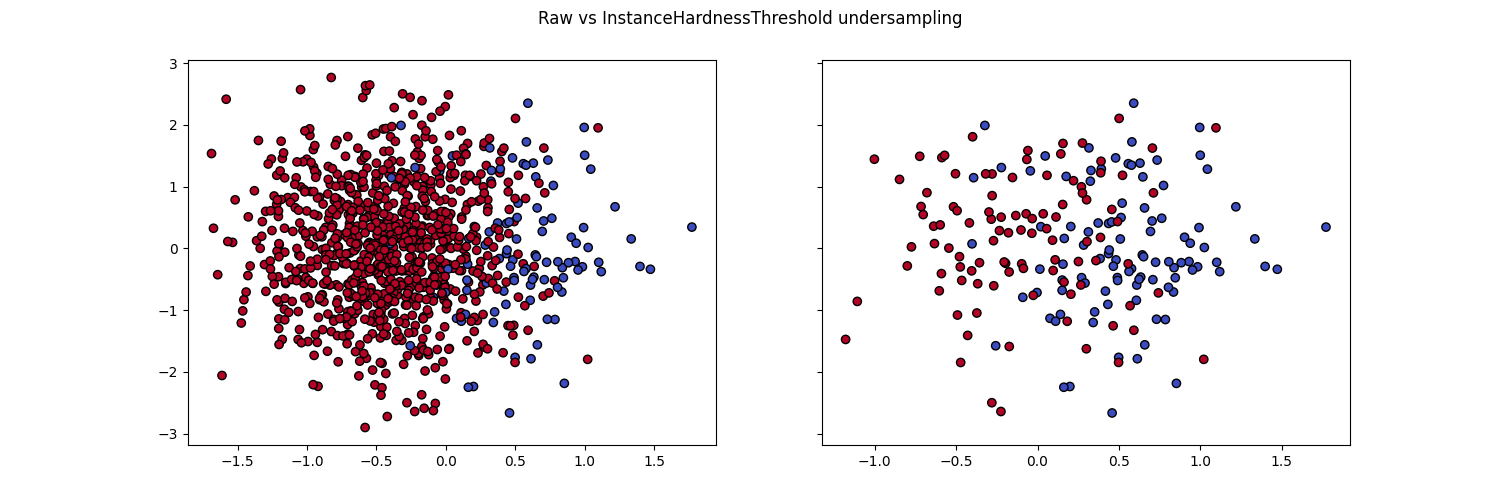
\includegraphics[width=1\textwidth]{images/Raw vs InstanceHardnessThreshold undersampling.png}
    \caption{InstanceHardnessThreshold örneği.}
    \label{fig:enter-label}
\end{figure}

\newpage
\section{Feature Selection}
Özellik seçimi, veri setindeki en önemli özellikleri belirleyerek, modelin daha iyi performans göstermesini sağlayan bir süreçtir. Bu süreçte, gereksiz veya düşük önemli özelliklerin filtrelenmesi ve modelin daha iyi genelleme yapabilmesini sağlayacak şekilde veri setinin basitleştirilmesi amaçlanır. Doğru özelliklerin seçilmesi, modelin doğruluğunu artırabilir ve gereksiz hesaplama maliyetlerini azaltabilir.

\begin{figure}[h]
    \centering
    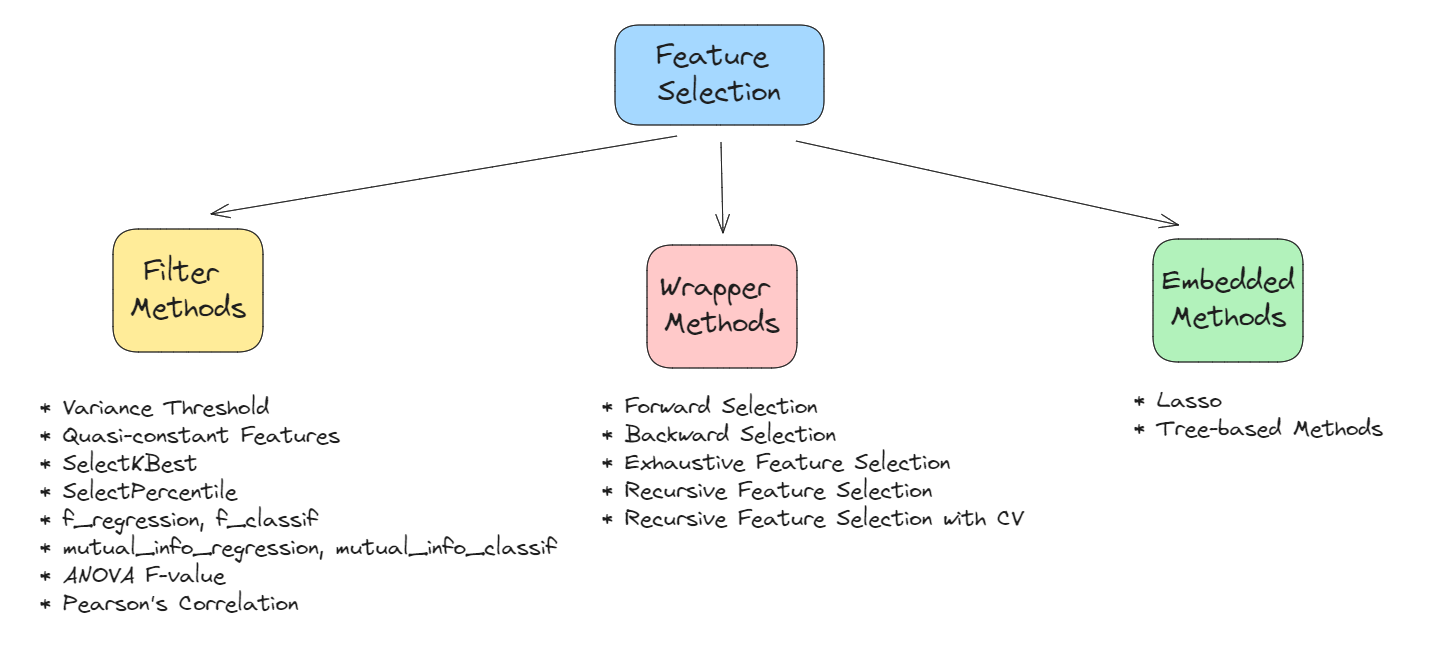
\includegraphics[width=1\textwidth]{images/feature_selection_methods.png}
    \caption{Özellik seçimi metodları.}
    \label{fig:enter-label}
\end{figure}

\subsection{Filter Methods (Filtre Yöntemleri)}
Filtre yöntemleri bir ön işleme adımı olarak kullanılır. Özelliklerin seçimi herhangi bir makine öğrenimi algoritmasından bağımsızdır. Bunun yerine, özellikler, sonuç değişkeniyle olan korelasyonlarına yönelik çeşitli istatistiksel testlerdeki puanlarına göre seçilir. Wrapper Methods (Sarmalayıcı Yöntemler)'den daha düşük tahmin performansı verirler. Hızlı bir tarama ve alakasız özelliklerin çıkarılması için çok uygundurlar.

\textbf{Variance Threshold (Varyans Eşiği):} Varyansı belirli bir eşiği karşılamayan tüm özellikleri kaldırır. Default olarak tüm sıfır varyanslı özellikleri kaldırır.

\begin{lstlisting}[language=Python]
from sklearn.feature_selection import VarianceThreshold
vt = VarianceThreshold(threshold=0).fit(X_train)

vt.get_support()
\end{lstlisting}

\textbf{Quasi-constant Features (Yarı sabit özellikler):} Yarı sabit özellikler, veri kümesindeki gözlemlerin büyük çoğunluğu için aynı değeri gösteren özelliklerdir. Bu özellikler, bir makine öğrenimi modelinin bir hedefi ayırt etmesine veya tahmin etmesine olanak tanıyan çok az bilgi sağlar. Ancak istisnalar da olabilir.

\begin{lstlisting}[language=Python]
from sklearn.feature_selection import VarianceThreshold
vt = VarianceThreshold(threshold=0.01).fit(X_train)

vt.get_support()
\end{lstlisting}

\textbf{SelectKBest:} Özellikleri en yüksek k puana göre seçer. Beraber Chi-square testi yapılabilir.

\begin{lstlisting}[language=Python]
from sklearn.feature_selection import SelectKBest, chi2
X_new = SelectKBest(chi2, k=3).fit_transform(X, y)
X_new.shape
\end{lstlisting}

\textbf{SelectPercentile:} En yüksek puanların yüzdelik dilimine göre özellikleri seçer.

\begin{lstlisting}[language=Python]
from sklearn.feature_selection import SelectPercentile, chi2
X_new = SelectPercentile(chi2, percentile=5).fit_transform(X, y)
X_new.shape
\end{lstlisting}

Regresyon problemleri için: f\_regression, mutual\_info\_regression
\begin{lstlisting}[language=Python]
f_value = f_regression(X_train, y_train)

for feature in zip(X_train.columns, f_value[0]):
	print(feature)

mi_score = mutual_info_regression(X_train, y_train)
for feature in zip(X_train.columns, mi_score):
	print(feature)
\end{lstlisting}

Sınıflandırma problemleri için: chi2, f\_classif, mutual\_info\_classif
\begin{lstlisting}[language=Python]
f_value = f_classif(X_train, y_train)

for feature in zip(X_train.columns, f_value[0]):
	print(feature)

mi_score = mutual_info_classif(X_train, y_train)
for feature in zip(X_train.columns, mi_score):
	print(feature)
\end{lstlisting}

F-testine dayalı yöntemler iki rastgele değişken arasındaki doğrusal bağımlılık derecesini tahmin eder. Karşılıklı bilgi yöntemleri (mutual\_ ile başlayanlar) her türlü istatistiksel bağımlılığı yakalayabilir ancak parametrik olmadıkları için doğru tahmin için daha fazla örneğe ihtiyaç duyarlar.

\begin{enumerate}
    \item \textbf{Information Gain (Karşılıklı Bilgi):} Bir özelliğin varlığının/yokluğunun hedef hakkında doğru tahminde bulunmaya ne kadar katkıda bulunduğunu ölçer. Bu değişkenlerden birini bilmenin diğer hakkıdaki belirsizliği ne kadar azalttığını ölçer. Örneğin X-Y bağımsızsa birini bilmenin diğeri hakkında bilgi vermez. Böylece information gain = 0'dır.
    \item \textbf{Fisher Score:} Negatif olmayan her özellik ve sınıf arasındaki ki-kare istatistiklerini hesaplar. Özellikler kategorik ise chi2 kullanılır.
    \item \textbf{ANOVA F-value:} Özellikler nicel ise her bir özellik ile hedef arasındaki ANOVA F-değeri hesaplanır. F-değeri, sayısal özelliği hedefe göre gruplandırdığımızda, her bir grubun ortalamalarının önemli ölçüde farklı olup olmadığını hesaplar.
    \item \textbf{Pearson Correlation:} Korelasyon, 2 veya daha fazla değişkenin doğrusal ilişkisinin bir ölçüsüdür. Korelasyon sayesinde bir değişkeni diğerinden tahmin edebiliriz. İyi değişkenler hedef değişkenle yüksek oranda ilişkilidir. Değişkenler hedef değişkenle ilişkili olmalı fakat kendi aralarında ilişkisiz olmalıdır. Eğer öyleyse, korelasyonlu olanlardan sadece birini tutmamız ve diğerlerini bırakmamız gerekir.
\end{enumerate}

\subsection{Wrapper Methods (Sarmalayıcı Yöntemler)}
Sarmalayıcı yöntemlerde, özelliklerin bir alt kümesini kullanmaya ve bunları kullanarak bir model eğitmeye çalışılır. Önceki modelden çıkardığımız çıkarımlara dayanarak, alt kümeye özellik eklemeye veya çıkarmaya karar verilir.

\textbf{Forward Selection:} Modelde hiçbir özellik olmadan başlanan iteratif bir yöntemdir. Her bir iterasyonda, yeni bir değişken eklenmesi modelin performansını iyileştirmeyene kadar modeli en iyi iyileştiren özelliği eklemeye devam eder.

\begin{lstlisting}[language=Python]
from mlxtend.feature_selection import SequentialFeatureSelector

sfs = SequentialFeatureSelector(RandomForestRegressor(), 
								   k_features=10, 
								   forward=True, 
								   floating=False, 
								   verbose=2,
								   scoring='r2',
								   cv=5)

sfs = sfs.fit(np.array(X_train), y_train)
sfs.k_feature_idx_
\end{lstlisting}

\textbf{Backward Selection:} Tüm özelliklerle başlanır ve her iterasyonda modelin performansını artıran en az anlamlı özellik kaldırılır. Bu işlem, özelliklerin kaldırılmasında herhangi bir iyileşme gözlenmeyene kadar tekrarlanır.

\begin{lstlisting}[language=Python]
from mlxtend.feature_selection import SequentialFeatureSelector

sfs = SequentialFeatureSelector(RandomForestRegressor(), 
								   k_features=10, 
								   forward=False, 
								   floating=False, 
								   verbose=2,
								   scoring='r2',
								   cv=5)

sfs = sfs.fit(np.array(X_train), y_train)
sfs.k_feature_idx_
\end{lstlisting}

\textbf{Exhaustive Feature Selection:} Bir algoritma için belirli bir performans metriğini optimize ederek tüm olası özellik alt kümeleri arasından en iyi özellik alt kümesi seçilir.\newline
\textbf{Recursive Feature Elimination:} En iyi performans gösteren özellik alt kümesini bulmayı amaçlayan açgözlü bir optimizasyon algoritmasıdır. Tekrar tekrar modeller oluşturur ve her iterasyonda en iyi veya en kötü performans gösteren özelliği bir kenarda tutar. Tüm özellikler tükenene kadar kalan özelliklerle bir sonraki modeli oluşturur. Daha sonra özellikleri eleme sırasına göre sıralar.\newline
\textbf{Recursive Feature Elimination with CV (RFECV):} 0 ile N özelliği yinelemeli olarak kaldırarak tahmin edici için en iyi özellik alt kümesini seçer.

\subsection{Embedded Methods (Gömülü Yöntemler)}
Lasso Regression: Lasso regresyonu, katsayıların büyüklüğünün mutlak değerlerine eşdeğer bir ceza ekleyen bir L1 düzenlemesi gerçekleştirir. L1, bazı katsayıları sıfıra kadar küçültebilen bir özelliğe sahiptir. Bu nedenle, bu özellik modelden çıkarılabilir.

\begin{lstlisting}[language=Python]
from sklearn.feature_selection import SelectFromModel
sel_ = SelectFromModel(Lasso(alpha=100))
sel_.fit(scaler.transform(X_train), y_train)
sel_.get_support()
\end{lstlisting}

Tree-based Methods: Ağaç modellerinin içerisindeki "feature\_importances\_" özelliği ile yapılır.
\begin{lstlisting}[language=Python]
rf = RandomForestClassifier().fit(X_train, y_train)
rf.feature_importances_
\end{lstlisting}

\newpage

\subsection{MAPIE (Model Agnostic Parameter Importance Estimation)}
Modelin türünden bağımsızdır.

\newpage
\section{Forecasting}
Zaman serisi analizi, zaman içinde gözlenen verileri incelemek ve bu verilerin gelecekteki değerlerini tahmin etmek amacıyla istatistiksel ve veri madenciliği tekniklerinin uygulanmasıdır. Zaman serisi verileri, belirli bir zaman diliminde toplanan verileri temsil eder ve genellikle düzenli zaman aralıklarıyla gözlenir.

Zaman Serisi Modelleri: ARIMA (Oto-Regressif Entegre Hareketli Ortalama), GARCH (Genelleştirilmiş Oto-Regressif Koşullu Heteroskedastiklik), Exponential Smoothing (Üssel Düzleştirme)

\subsection{Trend}
Trend, zaman içinde sürekli bir artış, azalış veya istikrarlı bir eğilimi ifade eder. Bu, bir zaman serisinin orta veya uzun vadeli değişimini temsil eder.

Hareketli Ortalama (Moving Average): Zaman serisindeki gürültüyü azaltmak ve trendi yakalamak için hareketli ortalama yöntemi kullanılabilir. Basit bir hareketli ortalama veya ağırlıklı hareketli ortalama kullanılabilir.
\begin{lstlisting}[language=Python]
# Basit bir hareketli ortalama hesaplama
rolling_mean = time_series.rolling(window=10).mean()
\end{lstlisting}

Lowess Düzleştirmesi: Lowess (Locally Weighted Scatterplot Smoothing) düzleştirmesi, veriyi yumuşatarak ve yerel eğilimleri yakalayarak trendi belirlemek için kullanılır.
\begin{lstlisting}[language=Python]
from statsmodels.nonparametric.smoothers_lowess import lowess

# Lowess duzlestirmesi ile trendi hesaplayin
smoothed = lowess(time_series, np.arange(len(time_series)), frac=0.2)

# Lowess duzlestirmesi sonuclarini gorsellestirin
plt.figure(figsize=(12, 6))
plt.plot(time_series, label="Zaman Serisi")
plt.plot(smoothed[:, 0], label="Trend (Lowess Duzlestirmesi)", linestyle="--")
plt.xlabel("Zaman")
plt.ylabel("Deger")
plt.legend()
plt.grid(True)
plt.show()
\end{lstlisting}

\newpage

\begin{figure}[h]
    \centering
    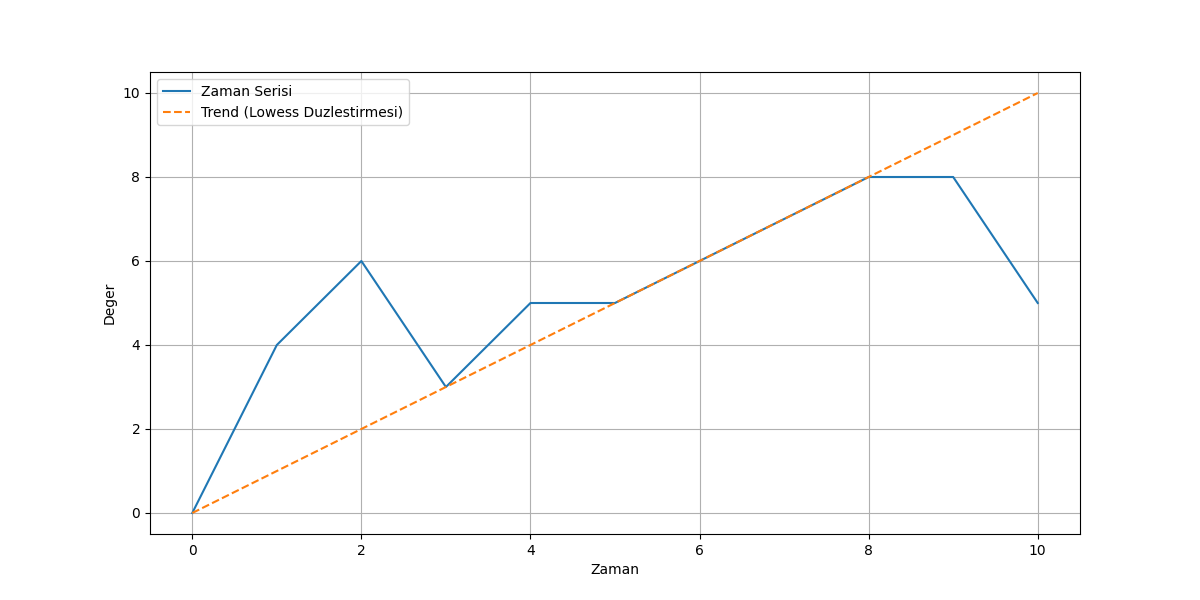
\includegraphics[width=0.8\textwidth]{images/lowess.png}
    \caption{Lowess düzleştirmesi örneği.}
    \label{fig:enter-label}
\end{figure}

\subsection{Durağanlık (Stationary)}
Durağanlık, bir zaman serisinin istatistiksel özelliklerinin zaman içinde sabit olduğu veya dalgalanmadığı bir durumu ifade eder. Durağan bir zaman serisi, ortalama, varyans ve otokorelasyon gibi özellikler açısından zaman içinde tutarlıdır. \textbf{Augmented Dickey-Fuller (ADF) Testi:} Bir test, bir zaman serisinin birim kök (unit root) varlığını veya yokluğunu belirlemeye yardımcı olur. Birim kök, zaman serisinin durağanlık özelliği olmadığını ifade eder. ADF testi, null hipotezi H0 ve alternatif hipotezi H1; H0 = Zaman serisi birim kök içerir ve durağan değildir. H1 = Zaman serisi birim kök içermez ve durağandır.

\begin{lstlisting}[language=Python]
import pandas as pd
from statsmodels.tsa.stattools import adfuller

# Ornek bir zaman serisi verisi olusturun
data = [10, 20, 30, 40, 50, 60, 70, 80, 90]

# Pandas Serisi olusturun
ts = pd.Series(data)

# ADF testini uygulayin
result = adfuller(ts)

# ADF test sonuclarini yazdirin
print('ADF Istatistigi:', result[0])
print('p-degeri:', result[1])
print('Kritik degerler:', result[4])

# Sonuclari yorumlayin
if result[1] <= 0.05:
    print('Zaman serisi duragan.')
else:
    print('Zaman serisi duragan degil.')
\end{lstlisting}

\textbf{Kwiatkowski-Philips-Schmidt-Shin (KPSS Testi):} H0: Zaman serisi, düzgün (trend-stationary) durağanlık gösterir. H1: Zaman serisi, düzgün durağanlık göstermez (durağanlık göstermeyen birim kök içerir.). KPSS testi, genellikle iki farklı sürümde uygulanır: düzgün durağanlık testi (Level Stationary Test) ve trend durağanlık testi (Trend Stationary Test).

\begin{enumerate}
    \item Düzgün Durağanlık Testi (Level Stationary Test): H0: Zaman serisi düzgün durağanlık gösterir. H1: Zaman serisi düzgün durağanlık göstermez.
    \item Trend Durağanlık Testi (Trend Stationary Test): H0: Zaman serisi eğimli durağanlık gösterir. H1: Zaman serisi eğimli durağanlık göstermez.
\end{enumerate}

\begin{lstlisting}[language=Python]
from statsmodels.tsa.stattools import kpss

# Ornek bir zaman serisi verisi olusturun
data = [10, 20, 30, 40, 50, 60, 70, 80, 90]

# Pandas Serisi olusturun
ts = pd.Series(data)

# Duzgun duraganlik testini uygulayin
kpss_stat_level, p_value_level, lags_level, critical_values_level = kpss(ts, regression='c')

# Trend duraganlik testini uygulayin
kpss_stat_trend, p_value_trend, lags_trend, critical_values_trend = kpss(ts, regression='ct')

# Duzgun duraganlik test sonuclarini yazdiri
print('Duzgun Duraganlik Test Istatistigi:', kpss_stat_level)
print('Duzgun Duraganlik Test p-degeri:', p_value_level)

# Trend duraganlik test sonuclarini yazdirin
print('Trend Duraganlik Test Istatistigi:', kpss_stat_trend)
print('Trend Duraganlik Test p-degeri:', p_value_trend)

# Sonuclari yorumlayin
if p_value_level <= 0.05:
    print('Zaman serisi duzgun duragan degil.')
else:
    print('Zaman serisi duzgun duragan.')

if p_value_trend <= 0.05:
    print('Zaman serisi trend duragan degil.')
else:
    print('Zaman serisi trend duragan.')
\end{lstlisting}

\textbf{Philips-Perron Testi:} Zaman serisinin eğilimsiz (trend-stationary) durağanlık özelliğini değerlendirmek için kullanılır. H0: Zaman serisi eğilimsiz durağanlık gösterir. H1: Zaman serisi eğilimsiz durağanlık göstermez.

\begin{lstlisting}[language=Python]
from statsmodels.tsa.stattools import adfuller

# Ornek bir zaman serisi verisi olusturun
data = [10, 20, 30, 40, 50, 60, 70, 80, 90]

# Pandas Serisi olusturun
ts = pd.Series(data)

# PP testini uygulayin
result = adfuller(ts, regression='ct')

# PP test sonuclarini yazdirin
print('PP Istatistigi:', result[0])
print('p-degeri:', result[1])
print('Kritik degerler:', result[4])

# Sonuclari yorumlayin
if result[1] <= 0.05:
    print('Zaman serisi egilimsiz duragan.')
else:
    print('Zaman serisi egilimsiz duragan degil.')
\end{lstlisting}

\textbf{Ljung-Box Testi:} Zaman serisinin otokorelasyonunu (kendi içindeki özbenzerliğini) test etmek için kullanılan bir istatistiksel testtir. Bu test, bir zaman serisinin rastgele gürültü içerip içeermediğini değerlendirmek amacıyla yaygın olarak kullanılır. Otokorelasyon, zaman serisinin kendisi ile belirli gecikmeler arasında pozitif veya negatif bir ilişki gösterip göstermediğini ölçer. H0: Zaman serisinin otokorelasyonu yoktur, yani zaman serisi bağımsızdır. H1: Zaman serisinde otokorelasyon vardır. Ljung-Box testi, belirli bir gecikme (lag) sayısı için bir test istatistiği hesaplar ve bu istatistiği karşılaştırılabilir bir eleştirel değerle karşılaştırır.

\begin{lstlisting}[language=Python]
from statsmodels.stats.diagnostic import acorr_ljungbox

# Ornek bir zaman serisi verisi olusturun
data = [10, 20, 30, 40, 50, 60, 70, 80, 90]

# Pandas Serisi olusturun
ts = pd.Series(data)

# Ljung-Box testini uygulayin
lags = 5  # Test edilecek gecikme sayisi
lb_stat, p_value = acorr_ljungbox(ts, lags=lags)

# Ljung-Box test sonuclarini yazdirin
print('Ljung-Box Istatistigi:', lb_stat)
print('p-degeri:', p_value)

# Sonuclari yorumlayin
if any(p_value <= 0.05):
    print('Zaman serisinde otokorelasyon vardir.')
else:
    print('Zaman serisinde otokorelasyon yoktur.')
\end{lstlisting}

\subsection{Mevsimsel (Seasonal) Değişkenler}
Mevsimsel değişkenler, belirli bir dönemde, düzenli aralıklarla tekrar eden belirli bir deseni ifade eder. Mevsimsel değişkenler, zaman serisinin mevsimsel etkilerini veya desenlerini yakalamak için kullanılır.\\
\textbf{Aralık Tablosu (Seasonal Decomposition of Time Series - STL):} Bu yöntem, zaman serisini trend, mevsimsel ve rastgele bileşenlere ayırmak için kullanılır.

\begin{lstlisting}[language=Python]
from statsmodels.tsa.seasonal import seasonal_decompose

# Zaman serisinin mevsimsel bilesenlerini cikartin
result = seasonal_decompose(time_series, model='additive')

# Mevsimsel bilesenleri gorsellestirin
result.seasonal.plot()
\end{lstlisting}

\textbf{ACF (Autocorrelation Function) ve PACF (Partial Autocorrelation Function):}

\begin{lstlisting}[language=Python]
from statsmodels.graphics.tsaplots import plot_acf, plot_pacf

# ACF grafigini cizdirin
plot_acf(time_series, lags=50)

# PACF grafigini cizdirin
plot_pacf(time_series, lags=50)
\end{lstlisting}

\textbf{Differencing (Fark Alma):} Zaman serisinde mevsimsel değişkenler varsa, veriyi fark alma (differencing) yöntemi kullanarak mevsimsel desenlerden arındırabilirsiniz. İlk fark, bir mevsimsel periyot boyunca (örneğin, bir yıl) yapılan farkı ifade eder. İkinci fark, ilk farkı fark alarak mevsimsel etkileri daha da azaltır.

\begin{lstlisting}[language=Python]
# Birinci fark
first_difference = time_series - time_series.shift(1)

# Ikinci fark
second_difference = first_difference - first_difference.shift(1)
\end{lstlisting}

\textbf{Exponential Smoothing (Üstel Düzleştirme):} Üstel düzleştirme yöntemleri (örneğin, Holt-Winters) mevsimsel değişkenleri modellemek için kullanılabilir. Bu yöntemler, verinin mevsimsel bileşenlerini ve mevsimsel desenlerini tahmin etmeye yardımcı olur.

\begin{lstlisting}[language=Python]
from statsmodels.tsa.holtwinters import ExponentialSmoothing

# Holt-Winters ustel duzlestirme modelini kullanarak mevsimsel degiskenleri tahmin edin
model = ExponentialSmoothing(time_series, seasonal='add', seasonal_periods=12)
result = model.fit()

# Mevsimsel tahminleri alin
seasonal_forecast = result.forecast(steps)
\end{lstlisting}

\textbf{Fourier Dönüşümleri:} Fourier dönüşümleri, mevsimsel desenleri modellendirmek için kullanılabilir. Bu yöntem, karmaşık mevsimsel desenleri yakalamak için sinüs ve kosinüs fonksiyonlarını kullanır.

\begin{lstlisting}[language=Python]
import numpy as np
import matplotlib.pyplot as plt
from scipy.fftpack import fft

# Ornek bir mevsimsel zaman serisi olusturun
t = np.linspace(0, 10, 1000) # Zaman araligi: 0-10 frequency = 0.2 # Mekanizmanin frekansi amplitude = 5 # Amplitud seasonal_component = amplitude * np.sin(2 * np.pi * frequency * t) # Mevsimsel bilesen
# Zaman serisini olusturun
time_series = np.random.randn(1000) + seasonal_component

# Zaman serisinin Fourier donusumunu alin
fourier_transform = fft(time_series)

# Fourier donusumunun buyuklugunu alin
magnitude = np.abs(fourier_transform)

# Mevsimsel frekansi bulun
seasonal_frequency = np.argmax(magnitude[1:]) / t[-1]  # Ilk eleman haric en buyuk magnitude'in indeksi

print(f"Mevsimsel frekans: {seasonal_frequency:.2f} periyot biriminde")

# Mevsimsel bileseni ayirin
seasonal_component = amplitude * np.sin(2 * np.pi * seasonal_frequency * t)

# Mevsimsel bilesen disindaki zaman serisini elde edin
non_seasonal_component = time_series - seasonal_component

# Mevsimsel bilesen ve geriye kalan zaman serisini gorsellestirin
plt.figure(figsize=(12, 6))
plt.plot(t, time_series, label="Mevsimsel Zaman Serisi")
plt.plot(t, seasonal_component, label="Mevsimsel Bilesen", linestyle="--")
plt.plot(t, non_seasonal_component, label="Mevsimsel Disi Bilesen", linestyle="--")
plt.xlabel("Zaman")
plt.ylabel("Deger")
plt.legend()
plt.grid(True)
plt.show()
\end{lstlisting}

\begin{figure}[h]
    \centering
    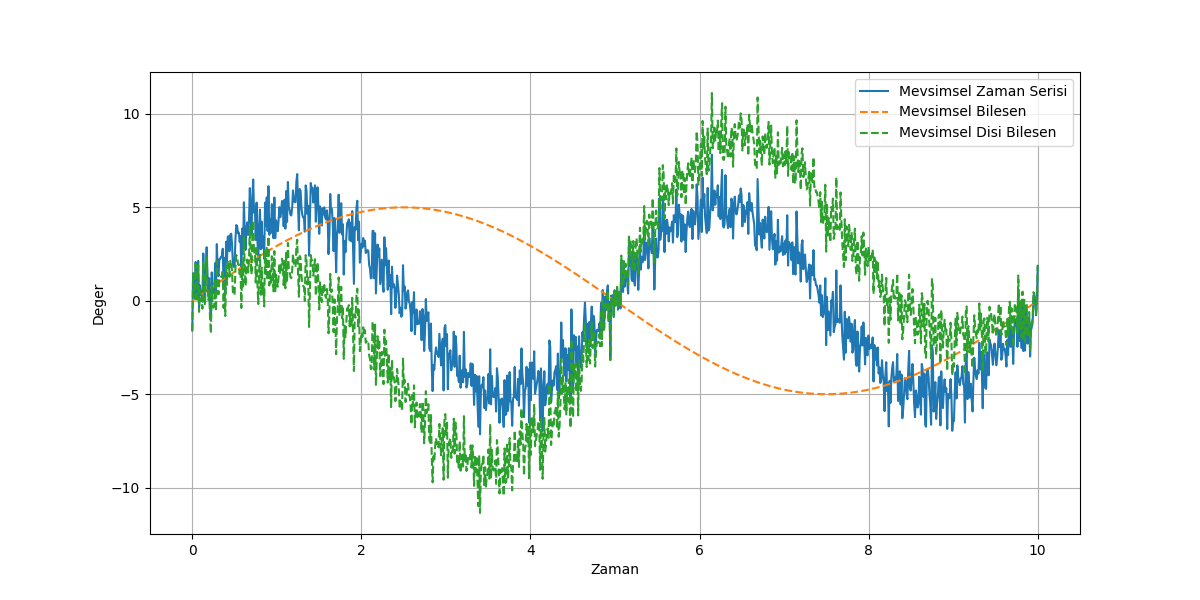
\includegraphics[width=0.7\textwidth]{images/fourier.png}
    \caption{Fourier dönüşümü örneği.}
    \label{fig:enter-label}
\end{figure}

\subsection{Rastgele Gürültü (Noise)}
Rastgele gürültü, zaman serisindeki tahmin edilemeyen, rastgele veya stokastik dalgalanmalardır. Genellikle, trend ve mevsimsel desenlerin dışında kalan değişkenliklerin neden olduğu dalgalanmalar olarak düşünülür. Rastgele gürültü, zaman serisindeki diğer bileşenlerin modelleme ve tahmininde dikkate alınmaz.

\newpage
\section{Gradient Boosting}
Toplu öğrenme yöntemidir. Modelin performansını geliştirmek için hatalara odaklanır.

\subsection{Çalışma Adımları}
\begin{enumerate}
    \item Temel bir model seçilir.
    \item Tüm veri seti için bir başlangıç tahmini yapılır. Regresyon için veri setinin ortalaması olabilir. Sınıflandırma için veri setindeki sınıfların oranı olabilir.
    \item Başlangıç tahmininden sonra, gerçek değerler ile başlangıç tahmin arasındaki hatalar hesaplanır. Bu hatalar, modelin daha fazla odaklanması gereken alanları gösterir.
    \item Hataların eğimi (gradient) hesaplanır. Eğim, her bir örnek için hata fonksiyonunun, tahmin edilen değerlere göre ne kadar değiştiğini gösterir.
    \item Bu hataları tahmin etmek için temel bir model oluşturur.
    \item Temel model, bir öğrenme oranı ile ağırlanır ve hata tahminine katılır. Öğrenme oranı, her temel modelin katkısını düzenler ve modelin aşırı uyumunu kontrol eder.
    \item Yeni temel modelin tahminleri, önceki tahminlere eklenir ve güncellenmiş bir tahmin elde edilir.
    \item İterasyon sayısına kadar 3 ve 7 arası tekrarlanır.
\end{enumerate}

\subsection{Hiperparametreler}
\begin{table}[h]
\centering
{\scriptsize\renewcommand{\arraystretch}{0.4}
{\resizebox*{\linewidth}{0.4\textwidth}{
\begin{tabular}{|p{3cm}|p{1cm}|p{1cm}|p{6cm}|}
\hline
Parametre & Type & Default & Açıklama \\ \hline
n\_estimators & int & 100 & Oluşturulacak temel modellerin sayısı. \\ \hline
learning\_rate & float & 0.1 & Her bir temel modelin katkısının ölçeği. \\ \hline
max\_depth & int & 3 & Oluşturulacak karar ağaçlarının maksimum derinliği. \\ \hline
min\_samples\_split & int & 2 & Bir iç düğümün ikiye bölünmeden önce kaç örneğe sahip olması gerektiği. \\ \hline
min\_samples\_leaf & int & 1 & Bir yaprak düğümünün en az kaç örneğe sahip olması gerektiği. \\ \hline
subsample & float & 1 & Her bir temel modelin eğitiminde kullanılacak örneklerin oranı. SGD'ye benzer bir etkiye sahiptir. \\ \hline

\end{tabular}
}}}
\end{table}

\newpage
\section{Grafik Türleri}
Veri bilimi, karmaşık veri setlerinden anlamlı bilgiler çıkarmak için çeşitli teknikler ve araçlar kullanır. Bu tekniklerden biri de grafiklerdir. Grafikler, verileri görsel olarak temsil ederek, desenleri ortaya çıkarır, ilişkileri gösterir ve bilgileri daha anlaşılır hale getirir.

\begin{figure}[h]
    \centering
    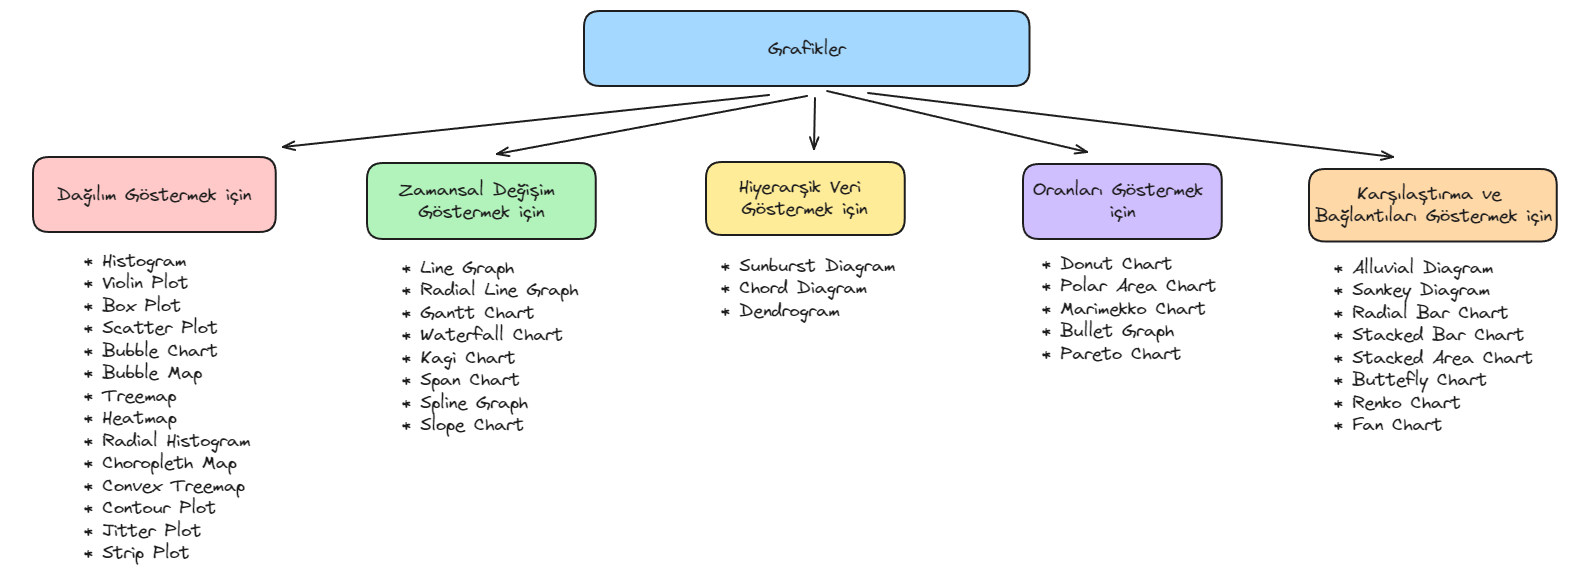
\includegraphics[width=1\textwidth]{images/graph_types.png}
    \caption{Grafik türleri.}
    \label{fig:enter-label}
\end{figure}

\newpage

\subsection{Alluvial Diagram}
Zamanla değişen kategorik değişkenler arasındaki ilişkileri göstermek için tercih edilirler. Değişkenler paralel olarak dikey eksene atanır. Değerler her eksende bloklarla gösterilir. Blok yüksekliği küme boyutunu, aradaki bağlantı yolu ise her iki blokta yer alan bileşenlerin boyutunu gösterir.

\begin{lstlisting}[language=Python]
import plotly.graph_objects as go

fig = go.Figure(data=[go.Sankey(
    node = dict(
      pad = 10,
      thickness = 25,
      line = dict(color = "black", width = 0.2),
      label = ["Satis", "Muhendislik", "Pazarlama"],
      color = "blue"
    ),
    link = dict(
      source = [2020, 2021, 2022],
      target = [1, 2, 3],
      value = [100, 120, 150],
  ))])

fig.update_layout(title_text="Sankey Diagram", font_size=10)
fig.show()
\end{lstlisting}

\begin{figure}[h]
    \centering
    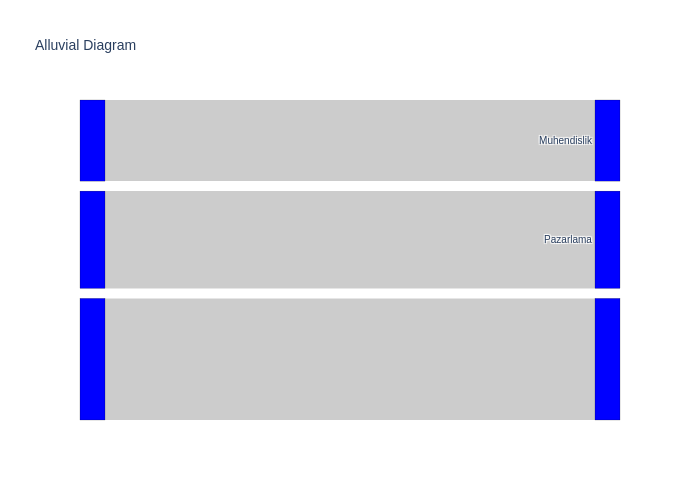
\includegraphics[width=0.8\textwidth]{images/alluvial_diagram.png}
    \caption{Alluvial diagram örneği.}
    \label{fig:enter-label}
\end{figure}

\newpage

\subsection{Sankey Diagram}
Akışları, ilişkileri ve kitleleri göstermek için kullanılır. Örneğin enerji akışları, bütçe dağılımları, materyal akışları, proses ilişkileri, kaynak dağılımı, bir sistemdeki akışlar vb. Okların kalınlığı akış miktarın, işlemler arasındaki ilişkiyi veya kaynakların dağılımı gösterir. Okların yönü, akışın hangi yönde olduğunu gösterir.

\begin{lstlisting}[language=Python]
import matplotlib.pyplot as plt
from matplotlib.sankey import Sankey

flows = [120, 80, 200, -180, -30, -70, -50]
labels = ['Giris', 'Islem 1', 'Islem 2', 'Islem 3', 'Islem 4', 'Islem 5', 'Cikis']

sankey = Sankey()
sankey.add(flows=flows, labels=labels, orientations=[0, 1, 1, -1, -1, -1, 0])
sankey.finish()

plt.title('Ornek Sankey Diagram')
plt.show()
\end{lstlisting}

\begin{figure}[h]
    \centering
    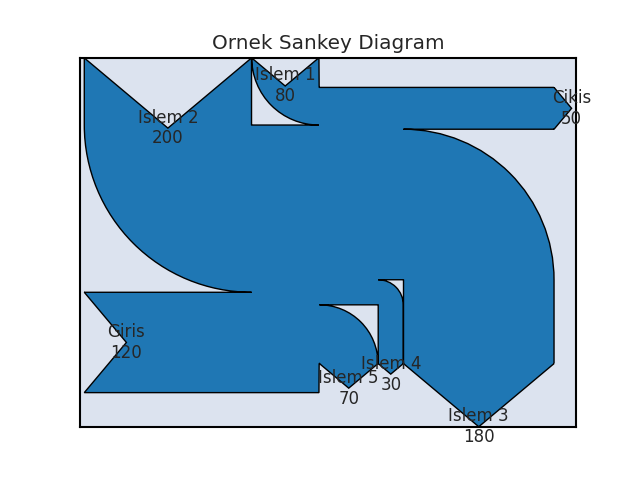
\includegraphics[width=0.7\textwidth]{images/sankey_diagram.png}
    \caption{Sankey diagram örneği.}
    \label{fig:enter-label}
\end{figure}

\newpage

\subsection{Donut Chart}
Pie chart'a benzer fakat ortası boştur. Kategorik bir bütünün parçalarının oransal dağılımını gösterir. Dilimi büyük olanın oransal dağılımı fazladır.

\begin{lstlisting}[language=Python]
import matplotlib.pyplot as plt

labels = ['A', 'B', 'C', 'D']
sizes = [25, 30, 20, 25]

fig, ax = plt.subplots()
ax.pie(sizes, labels=labels, autopct='%1.1f%%', startangle=90, wedgeprops=dict(width=0.3))
ax.axis('equal')

plt.title('Ornek Donut Chart')
plt.show()
\end{lstlisting}

\begin{figure}[h]
    \centering
    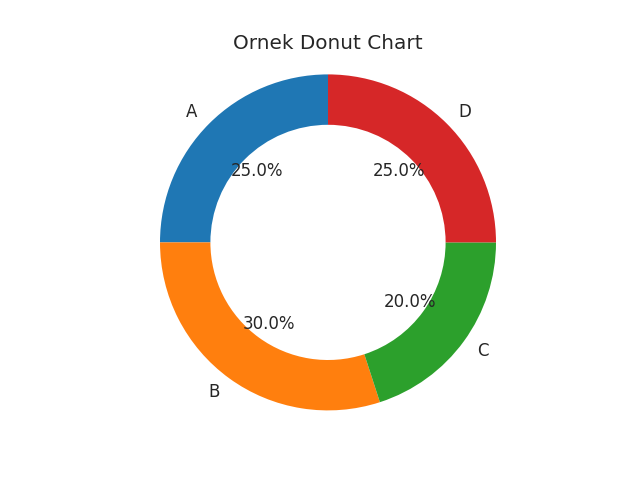
\includegraphics[width=0.7\textwidth]{images/donut_chart.png}
    \caption{Donut chart örneği.}
    \label{fig:enter-label}
\end{figure}

\newpage

\subsection{Line Graph}
Sürekli bir değişkenin belirli aralıklarla ölçülen veya zamanla değişen değerlerini göstermek için kullanılır.

\begin{lstlisting}[language=Python]
import matplotlib.pyplot as plt

x = [1, 2, 3, 4, 5]
y = [10, 15, 13, 18, 20]

plt.plot(x, y, marker='o', linestyle='-')

plt.title('Ornek Line Graph')
plt.xlabel('X Ekseni')
plt.ylabel('Y Ekseni')
plt.grid(True)
plt.show()

\end{lstlisting}

\begin{figure}[h]
    \centering
    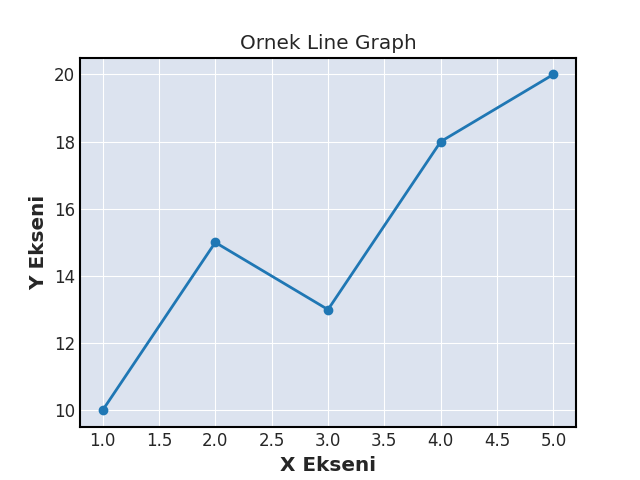
\includegraphics[width=0.7\textwidth]{images/line_graph.png}
    \caption{Line graph örneği.}
    \label{fig:enter-label}
\end{figure}

\newpage

\subsection{Radial Bar Chart}
Birbirine bağlı veya ilişkili kategorik verileri karşılaştırmak için kullanılır.

\begin{lstlisting}[language=Python]
import matplotlib.pyplot as plt
import numpy as np

categories = ['A', 'B', 'C', 'D']
values = [20, 35, 30, 25]

angles = np.linspace(0, 2 * np.pi, len(categories), endpoint=False).tolist()

fig, ax = plt.subplots(figsize=(6, 6), subplot_kw=dict(polar=True))
bars = ax.bar(angles, values, width=0.5, color='skyblue', edgecolor='black')

ax.set_xticks(angles)
ax.set_xticklabels(categories)

plt.title('Ornek Radial Bar Chart')
plt.show()
\end{lstlisting}

\begin{figure}[h]
    \centering
    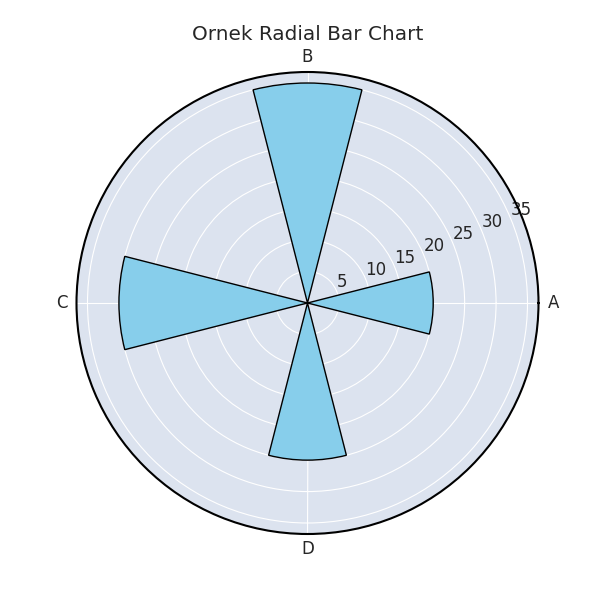
\includegraphics[width=0.7\textwidth]{images/radial_bar_chart.png}
    \caption{Radial bar chart örneği.}
    \label{fig:enter-label}
\end{figure}

\newpage

\subsection{Polar Area Chart}
Verilerin oransal dağılımını göstermek için kullanılır.

\begin{lstlisting}[language=Python]
import matplotlib.pyplot as plt

categories = ['A', 'B', 'C', 'D']
values = [20, 35, 30, 25]

fig, ax = plt.subplots(figsize=(6, 6), subplot_kw=dict(polar=True))
bars = ax.bar(categories, values, width=0.5, color='skyblue')

plt.title('Ornek Polar Area Chart')
plt.show()
\end{lstlisting}

\begin{figure}[h]
    \centering
    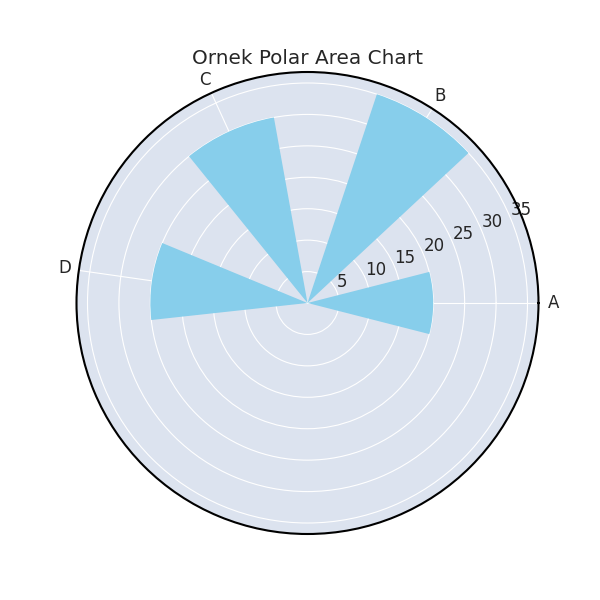
\includegraphics[width=0.7\textwidth]{images/polar_area_chart.png}
    \caption{Polar area örneği.}
    \label{fig:enter-label}
\end{figure}

\newpage

\subsection{Bar Chart}
Kategorik verilerin sayısal değerlerini göstermek için kullanılır.

\begin{lstlisting}[language=Python]
import matplotlib.pyplot as plt

categories = ['A', 'B', 'C', 'D']
values = [20, 35, 30, 25]

plt.figure(figsize=(8, 6))
plt.bar(categories, values, color='skyblue')

plt.title('Ornek Bar Chart')
plt.xlabel('Kategoriler')
plt.ylabel('Degerler')
plt.show()
\end{lstlisting}

\begin{figure}[h]
    \centering
    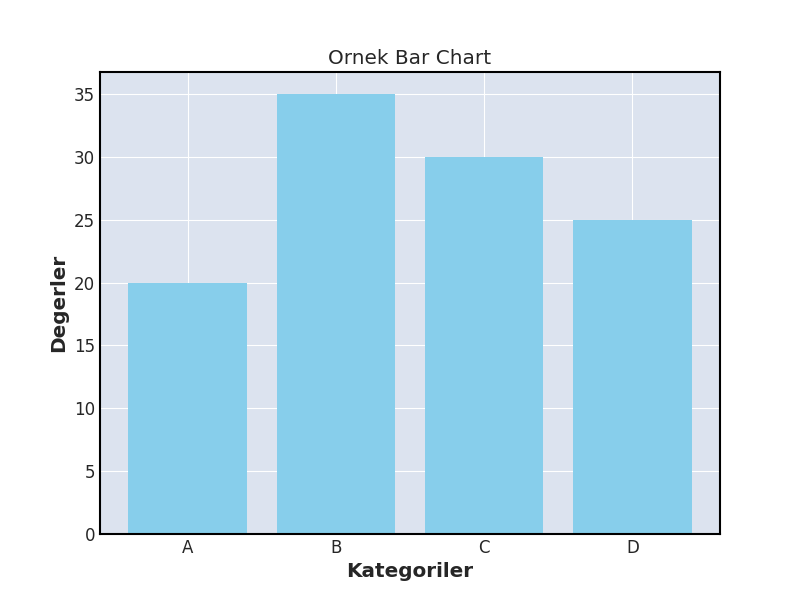
\includegraphics[width=0.7\textwidth]{images/bar_chart.png}
    \caption{Bar chart örneği.}
    \label{fig:enter-label}
\end{figure}

\newpage

\subsection{Radial Histogram}
Özellikle dairesel veya halka şeklindeki veri yapısını vurgulamak ve veri setinin yoğunluk veya dağılımını görsel olarak göstermek için kullanılır.

\begin{lstlisting}[language=Python]
import matplotlib.pyplot as plt
import numpy as np

np.random.seed(0)
r = np.random.normal(0, 1, 1000)
theta = 2 * np.pi * np.random.rand(1000)

plt.figure(figsize=(6, 6))
plt.hist(theta, bins=30, color='skyblue')

plt.title('Ornek Radial Histogram')
plt.show()
\end{lstlisting}

\begin{figure}[h]
    \centering
    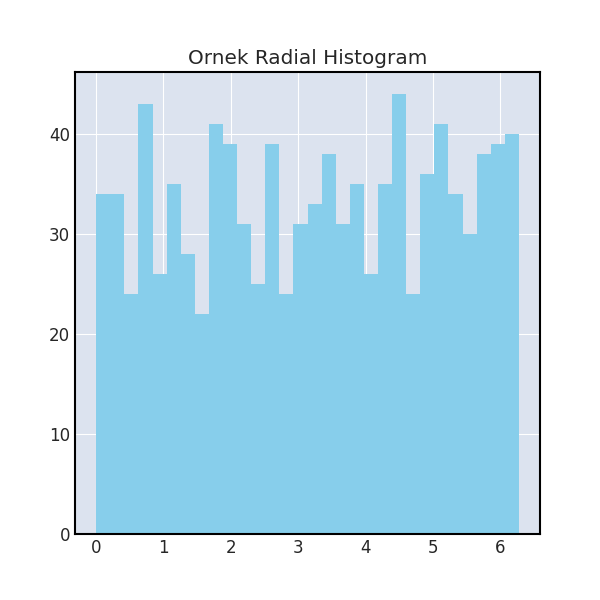
\includegraphics[width=0.7\textwidth]{images/radial_histogram.png}
    \caption{Radial histogram örneği.}
    \label{fig:enter-label}
\end{figure}

\newpage

\subsection{Sunburst Diagram}
Bir bütün parçalarını ve parçaların hiyerarşik yapılarını göstermek için kullanılır. Kategorik verilerin alt kategorilerle ilişkisini ve her bir kategorinin toplam içindeki oransal büyüklüğünü vurgulamak için tercih edilir.

\begin{lstlisting}[language=Python]
import plotly.graph_objects as go

fig = go.Figure(go.Sunburst(
    labels=["A", "B", "C", "D", "E", "F"],
    parents=["", "A", "B", "B", "C", "C"],
    values=[10, 15, 8, 7, 12, 5],
))

fig.update_layout(title='Ornek Sunburst Diagram')
fig.show()
\end{lstlisting}

\begin{figure}[h]
    \centering
    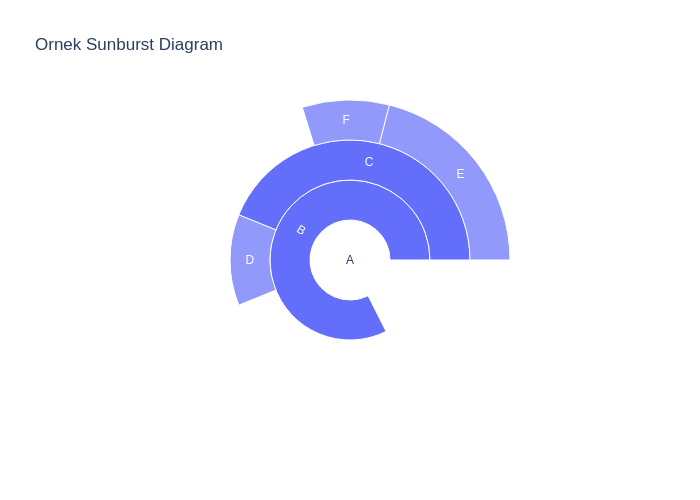
\includegraphics[width=0.7\textwidth]{images/sunburst_diagram.png}
    \caption{Sunburst diagram örneği.}
    \label{fig:enter-label}
\end{figure}

\newpage

\subsection{Treemap}
Hiyerarşik verileri dikdörtgen kutuların alanları olarak görselleştiren bir grafik türüdür. Bir bütünün parçalarını ve parçaların hiyerarşik yapılarını göstermek için kullanılır.

\begin{lstlisting}[language=Python]
import matplotlib.pyplot as plt
import squarify

sizes = [25, 30, 20, 15, 10]

squarify.plot(sizes=sizes, label=["A", "B", "C", "D", "E"], alpha=0.7)

plt.title('Ornek Treemap')
plt.axis('off')
plt.show()
\end{lstlisting}

\begin{figure}[h]
    \centering
    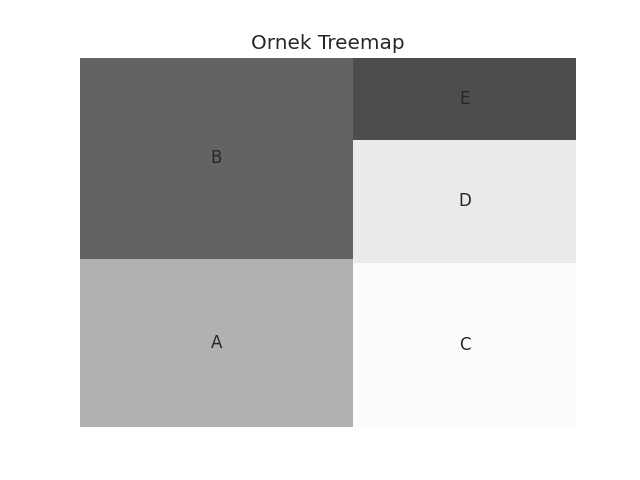
\includegraphics[width=0.7\textwidth]{images/treemap.png}
    \caption{Treemap örneği.}
    \label{fig:enter-label}
\end{figure}

\newpage

\subsection{Heatmap}
Sayısal verilerin yoğunluğu veya ilişkilerini renklerle göstermek için kullanılır. Her bir hücre, veri setindeki bir iki değişken arasındaki ilişki değerini temsil eder.

\begin{lstlisting}[language=Python]
import seaborn as sns
import numpy as np

data = np.random.rand(10, 10)

sns.heatmap(data, cmap='YlGnBu')

plt.title('Ornek Heatmap')
plt.show()
\end{lstlisting}

\begin{figure}[h]
    \centering
    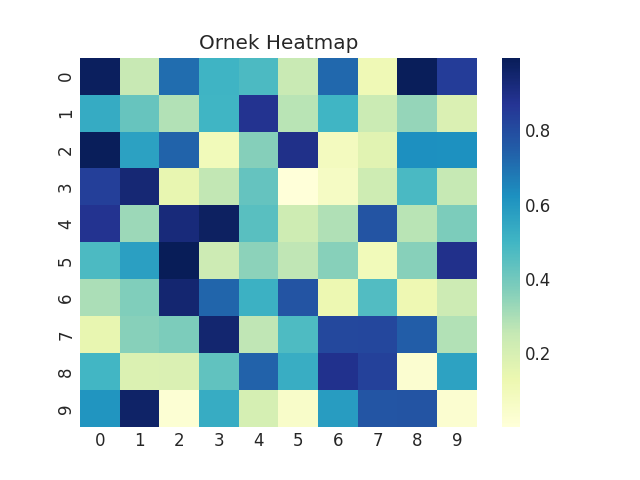
\includegraphics[width=0.7\textwidth]{images/heatmap.png}
    \caption{Heatmap örneği.}
    \label{fig:enter-label}
\end{figure}

\newpage

\subsection{Stacked Bar Chart}
Kategorik verilerin karşılaştırılması için kullanılır. Farklı kategoriler içindeki alt kategorilerin değerlerini karşılaştırmak için kullanılır.

\begin{lstlisting}[language=Python]
import matplotlib.pyplot as plt

categories = ['A', 'B', 'C', 'D']
values1 = [20, 35, 30, 25]
values2 = [15, 25, 20, 15]

plt.figure(figsize=(8, 6))
plt.bar(categories, values1, color='skyblue', label='Grup 1')
plt.bar(categories, values2, bottom=values1, color='orange', label='Grup 2')

plt.title('Ornek Stacked Bar Chart')
plt.xlabel('Kategoriler')
plt.ylabel('Degerler')
plt.legend()
plt.show()
\end{lstlisting}

\begin{figure}[h]
    \centering
    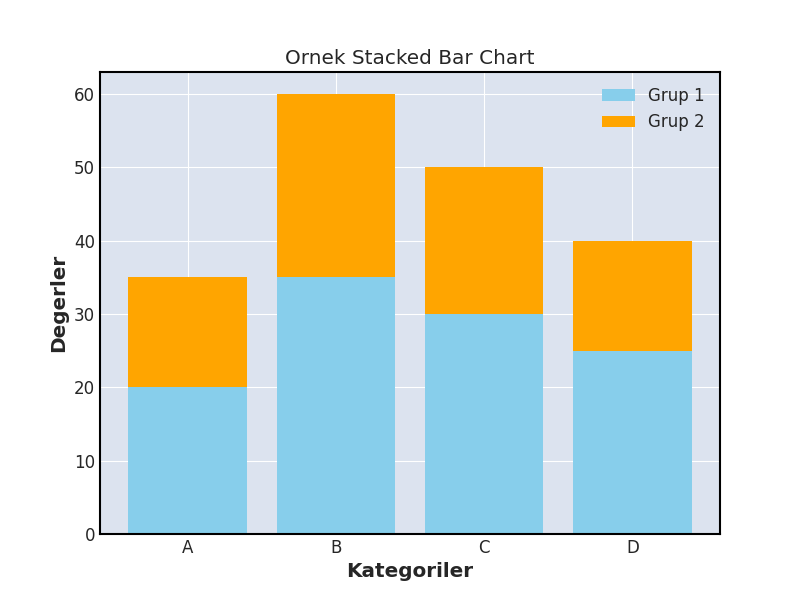
\includegraphics[width=0.7\textwidth]{images/stacked_bar_chart.png}
    \caption{Stacked bar chart örneği.}
    \label{fig:enter-label}
\end{figure}

\newpage

\subsection{Chord Diagram}
İlişkisel verileri ve bu veriler arasındaki bağlantıları daire içindeki yaylarla gösterir.

\begin{lstlisting}[language=Python]
import matplotlib.pyplot as plt
from matplotlib.sankey import Sankey

links = {
    ("A", "B"): 20,
    ("A", "C"): 15,
    ("B", "C"): 25,
    ("B", "D"): 10,
    ("C", "D"): 30
}

fig, ax = plt.subplots(figsize=(8, 8))
sankey = Sankey(ax=ax)
for link, weight in links.items():
    sankey.add(flows=[weight, -weight], labels=list(link))
sankey.finish()

plt.title('Ornek Chord Diagram')
plt.show() 
\end{lstlisting}

\begin{figure}[h]
    \centering
    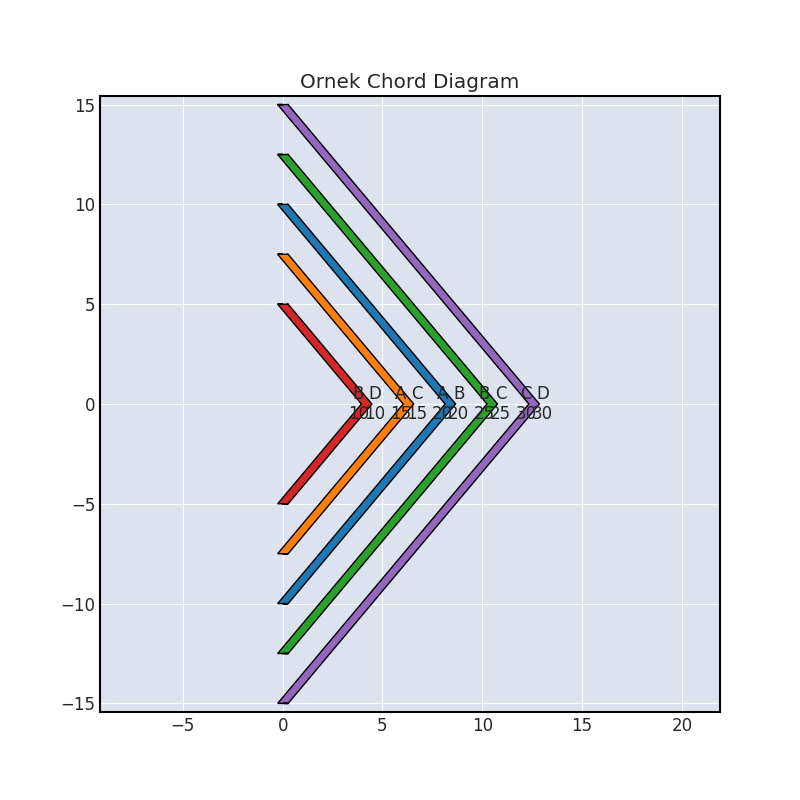
\includegraphics[width=0.6\textwidth]{images/chord_diagram.png}
    \caption{Chord diagram örneği.}
    \label{fig:enter-label}
\end{figure}

\newpage

\subsection{Choropleth Map}
Belirli bir coğrafi alandaki veri desenlerini, dağılımları veya farklılıkları görsel olarak anlamak için kullanılır.

\begin{lstlisting}[language=Python]
import geopandas as gpd
import random
import matplotlib.pyplot as plt

world = gpd.read_file(gpd.datasets.get_path('naturalearth_lowres'))

data = {country: random.randint(1, 10) for country in world['name']}
world['data'] = world['name'].map(data)

world.plot(column='data', cmap='YlOrRd', legend=True, figsize=(15, 10))
plt.title('Ornek Choropleth Harita')
plt.show() 
\end{lstlisting}

\begin{figure}[h]
    \centering
    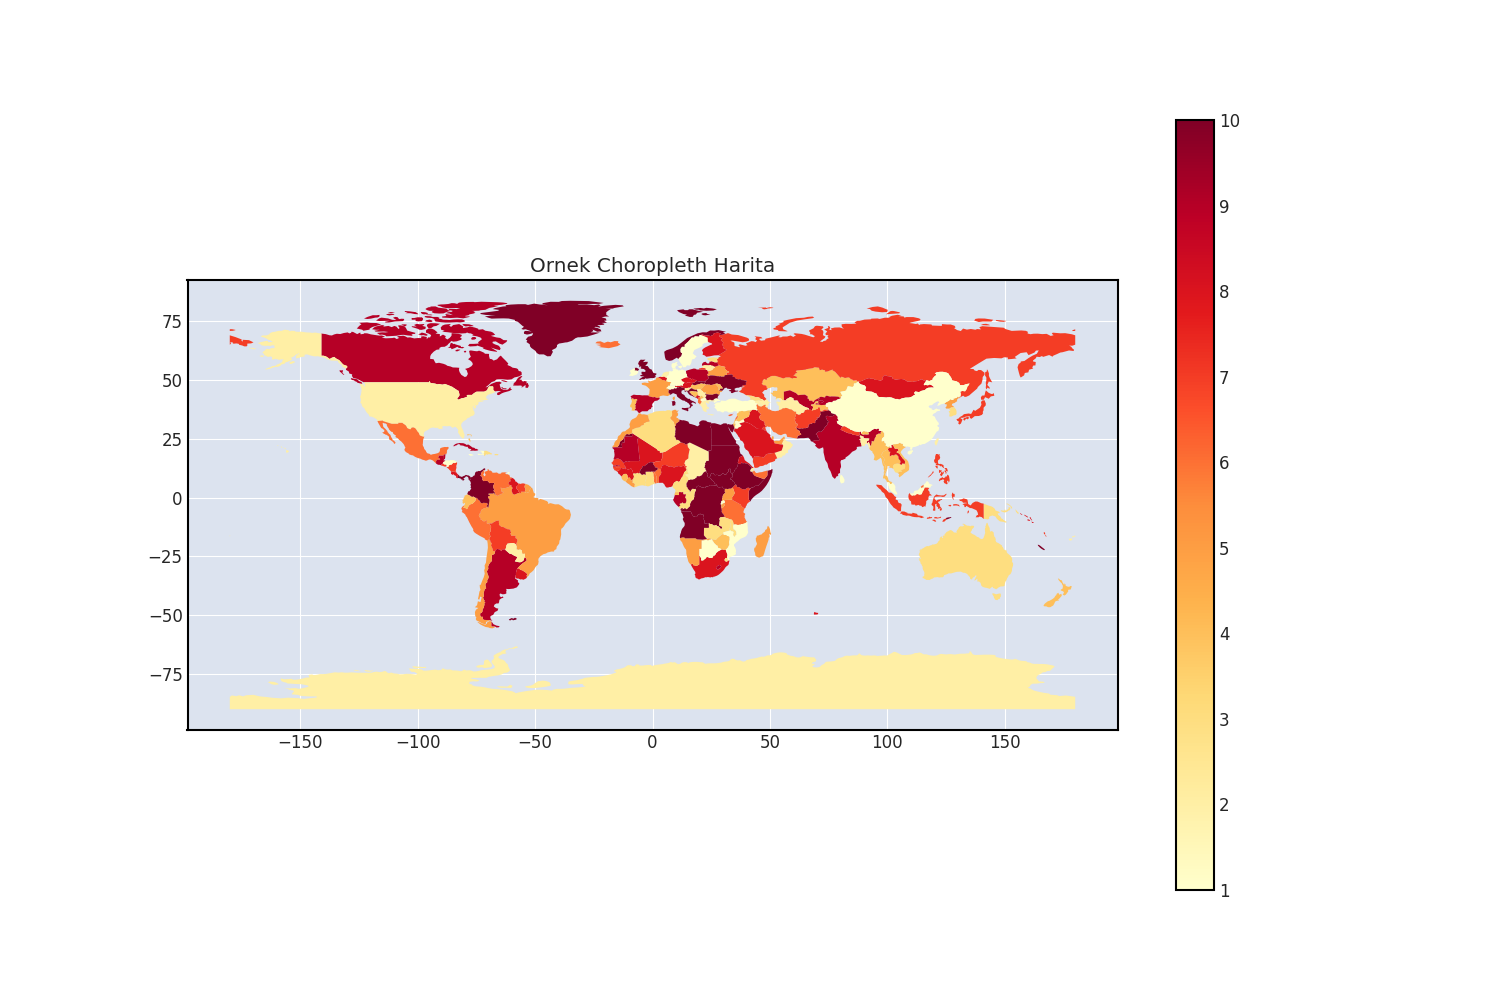
\includegraphics[width=0.7\textwidth]{images/choropleth_map.png}
    \caption{Choropleth map örneği.}
    \label{fig:enter-label}
\end{figure}

\newpage

\subsection{Radial Line Graph}
Genellikle zaman içinde değişen veya belirli bir dönemde farklı bir kategoriler arasındaki ilişkiyi göstermek için kullanılır. Her bir çizgi, bir kategori veya değişkeni, çizgilerin uzunlukları veri değerlerini temsil eder.

\begin{lstlisting}[language=Python]
import matplotlib.pyplot as plt
import numpy as np

categories = ['A', 'B', 'C', 'D']
values = [10, 20, 15, 25]

fig, ax = plt.subplots(subplot_kw=dict(polar=True))

theta = np.linspace(0, 2 * np.pi, len(categories), endpoint=False)
values += values[:1]
theta += theta[:1]

ax.plot(theta, values, marker='o')

ax.set_theta_offset(np.pi / 2)
ax.set_theta_direction(-1)

plt.title('Ornek Radial Line Graph')
plt.show()
\end{lstlisting}

\begin{figure}[h]
    \centering
    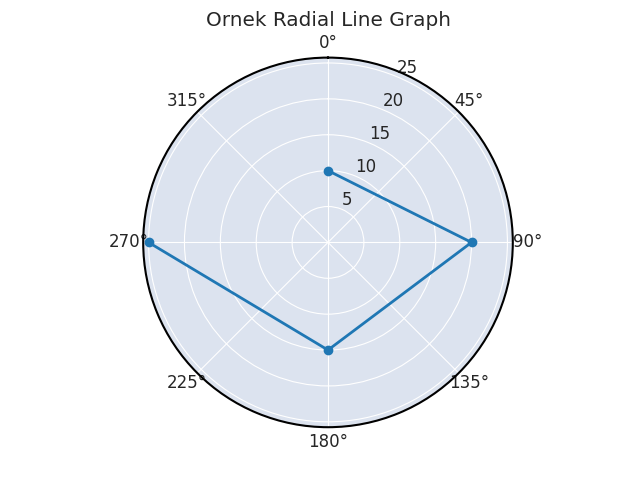
\includegraphics[width=0.7\textwidth]{images/radial_line_graph.png}
    \caption{Radial line örneği.}
    \label{fig:enter-label}
\end{figure}

\newpage

\subsection{Bubble Map}
Coğrafi bölgelerin veya noktaların harita üzerinde farklı büyüklükte veya renklerde dairelerle temsil edildiği bir harita türüdür.

\begin{lstlisting}[language=Python]
import plotly.express as px

data = dict(
    lat=[40.7128, 34.0522, 41.8781],
    lon=[-74.0060, -118.2437, -87.6298],
    text=['New York', 'Los Angeles', 'Chicago'],
    size=[20, 50, 30],
    color=[10, 20, 30]
)

fig = px.scatter_geo(data, lat='lat', lon='lon', text='text', size='size', color='color')
fig.update_geos(projection_type="natural earth")

fig.update_layout(title='Ornek Bubble Map')
fig.show()
\end{lstlisting}

\begin{figure}[h]
    \centering
    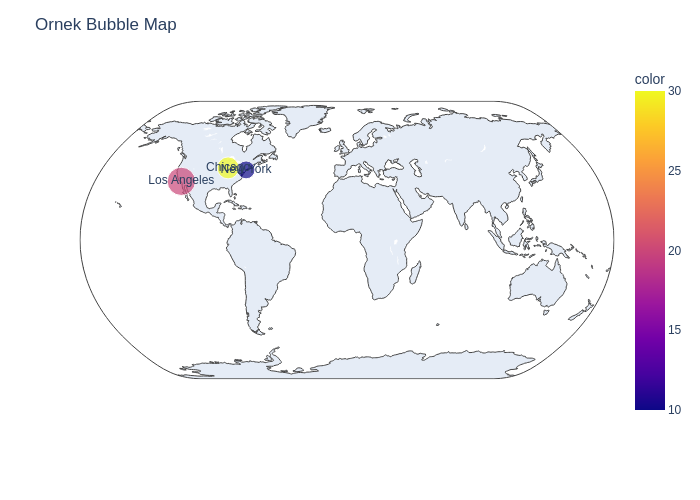
\includegraphics[width=0.7\textwidth]{images/bubble_map.png}
    \caption{Bubble map örneği.}
    \label{fig:enter-label}
\end{figure}

\newpage

\subsection{Bubble Chart}
İki değişken arasındaki ilişkiyi gösteren bir scatter plot ile birlikte üçüncü bir değişkenin büyüklüğünü veya yoğunluğunu da gösterir. Her bir nokta bir veri noktasını temsil ederken, noktanın büyüklüğü veya renk tonu üçünü değişkeni gösterir.

\begin{lstlisting}[language=Python]
import matplotlib.pyplot as plt

x = [1, 2, 3, 4, 5]
y = [10, 15, 20, 25, 30]
sizes = [40, 80, 120, 160, 200]

plt.scatter(x, y, s=sizes, alpha=0.5)

plt.title('Ornek Bubble Chart')
plt.xlabel('X Degiskeni')
plt.ylabel('Y Degiskeni')
plt.show()
\end{lstlisting}

\begin{figure}[h]
    \centering
    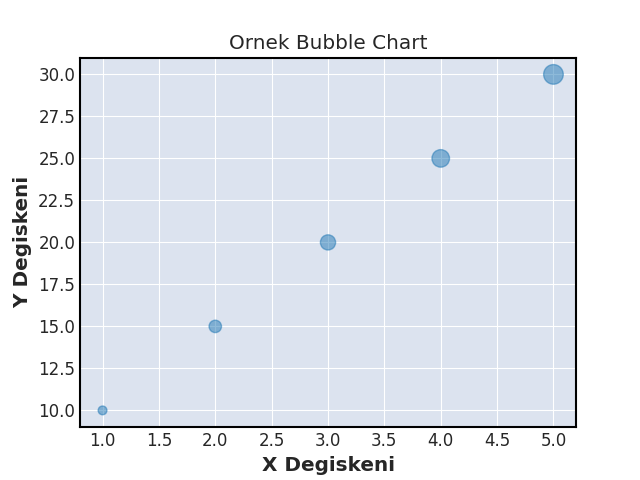
\includegraphics[width=0.7\textwidth]{images/bubble_chart.png}
    \caption{Bubble chart örneği.}
    \label{fig:enter-label}
\end{figure}

\newpage

\subsection{Violin Plot}
Box plot dağılım özelliklerini daha ayrıntılı bir şekilde gösterir. Her bir violin plot, verinin yoğunluk dağılımını gösteren bir çizgi plot ile birlikte simetriği bozulmuş bir kutu grafikten oluşur. Genellikle sayısal veri setlerindeki dağılımları veya gruplar arasındaki farklılıkları görselleştirmek için kullanılır. Özellikle veri dağılımının genel yapısal özellikleri, merkezi eğilim, değişkenlik ve simetriği hakkında bilgi verir. Daha geniş bölgelerde daha fazla veri bulunur. İçindeki kutu grafik, verinin dört çeyreği ve medyanı temsil eder. Gruplar arasındaki veri dağılımını ve merkezi eğilim farklarını hızlıca karşılaştırmak için kullanılır.

\begin{lstlisting}[language=Python]
import seaborn as sns
import matplotlib.pyplot as plt

tips = sns.load_dataset("tips")

sns.violinplot(x="day", y="total_bill", data=tips)

plt.title('Ornek Violin Plot')
plt.xlabel('Gun')
plt.ylabel('Toplam Fatura')
plt.show()
\end{lstlisting}

\begin{figure}[h]
    \centering
    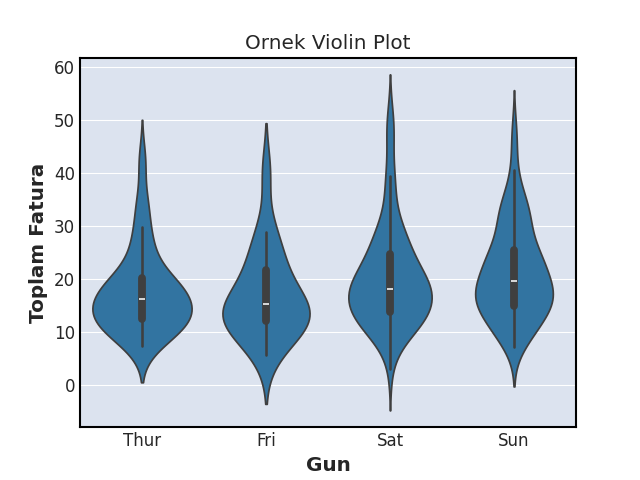
\includegraphics[width=0.7\textwidth]{images/violin_plot.png}
    \caption{Violin plot örneği.}
    \label{fig:enter-label}
\end{figure}

\newpage

\subsection{Box Plot}
Sayısal veri setlerinin dağılımını, merkezi eğilimini ve değişkenliğini görselleştirmek için kullanılan bir grafik türüdür. Veri setinin beş numaralı özeti (five number summary: minimum, birinci çeyrek, medyan, üçüncü çeyrek, maksimum) üzerine odaklanır. Gruplar arasındaki farklılıkları karşılaştırmak veya aykırı değerleri belirlemek için kullanılır. Kutunun alt sınırı birinci çeyrek (Q1), üst sınırı üçüncü çeyrek (Q3), ortadaki çizgi medyanı temsil eder. Kutunun uzunluğu verinin çeyrekler arası genişliğini (verinin yayılımını) gösterir. Aykırı değerler, alt veya üst sınırın dışında yer alan noktalar olarak gösterilir.

\begin{lstlisting}[language=Python]
import seaborn as sns
import matplotlib.pyplot as plt

tips = sns.load_dataset("tips")

sns.boxplot(x="day", y="total_bill", data=tips)
plt.title('Ornek Box Plot')
plt.xlabel('Gun')
plt.ylabel('Toplam Fatura')
plt.show()
\end{lstlisting}

\begin{figure}[h]
    \centering
    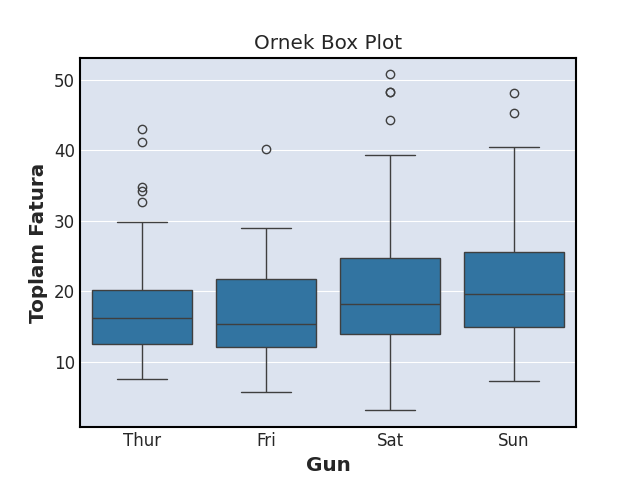
\includegraphics[width=0.7\textwidth]{images/box_plot.png}
    \caption{Box plot örneği.}
    \label{fig:enter-label}
\end{figure}

\newpage

\subsection{Stacked Area Chart}
Zamanla değişen kategorik verilerin toplamını veya oransal dağılımını görselleştirmek için kullanılır. Grafiğin üst kısmındaki toplam alan, tüm kategorilerin toplam değerini gösterir.

\begin{lstlisting}[language=Python]
import matplotlib.pyplot as plt

categories = ['Kategori 1', 'Kategori 2', 'Kategori 3']
values1 = [20, 30, 25]
values2 = [15, 25, 30]
values3 = [25, 20, 10]

plt.stackplot(categories, values1, values2, values3, labels=['Grup 1', 'Grup 2', 'Grup 3'])
plt.legend(loc='upper left')
plt.title('Ornek Stacked Area Chart')
plt.xlabel('Kategoriler')
plt.ylabel('Degerler')
plt.show()
\end{lstlisting}

\begin{figure}[h]
    \centering
    \includegraphics[width=0.7\textwidth]{images/stacked_area_chart.png}
    \caption{Stacked area chart örneği.}
    \label{fig:enter-label}
\end{figure}

\newpage

\subsection{Gantt Chart}
İş akışı sürecindeki görevlerin, aktivitelerin veya işlerin zaman içindeki ilerleyişini ve zamanlamasını temsil eder. Her bir çubuğun uzunluğu görevin ne kadar sürede tamamlanacağını gösterir. Çubukların başlangıç ve bitiş zamanları, ilgili görevlerin zamanlamasını gösterir.

\begin{lstlisting}[language=Python]
import plotly.figure_factory as ff

data = [
    dict(Task="Gorev 1", Start='2023-01-01', Finish='2023-01-31'),
    dict(Task="Gorev 2", Start='2023-02-01', Finish='2023-03-15'),
    dict(Task="Gorev 3", Start='2023-02-15', Finish='2023-04-10'),
]

fig = ff.create_gantt(data)
fig.show()
\end{lstlisting}

\begin{figure}[h]
    \centering
    \includegraphics[width=0.7\textwidth]{images/gantt_chart.png}
    \caption{Gantt chart örneği.}
    \label{fig:enter-label}
\end{figure}

\newpage

\subsection{Dot Plot}
Her bir veri noktasını temsil etmek için noktalar kullanılır. Kategorik veya sayısal verilerin frekanslarını veya değerlerini görselleştirmek için kullanılır. Noktaların yoğun olduğu bölgeler, o değerin veri setinde daha sık veya yoğun olduğunu gösterir. Veri setinin dağılımını anlamak için kullanılır.

\begin{lstlisting}[language=Python]
import seaborn as sns
import matplotlib.pyplot as plt

data = [5, 7, 8, 7, 2, 17, 2, 9, 4, 11, 12, 9, 6]

sns.stripplot(data, jitter=True, marker='o', alpha=0.5)

plt.title('Ornek Dot Plot')
plt.xlabel('Degerler')
plt.show()
\end{lstlisting}

\begin{figure}[h]
    \centering
    \includegraphics[width=0.7\textwidth]{images/dot_plot.png}
    \caption{Dot plot örneği.}
    \label{fig:enter-label}
\end{figure}

\newpage

\subsection{Scatter Plot}
İki sayısal değişken arasındaki ilişkiyi görselleştirmek için kullanılır. Veri noktalarının dağılımını, korelasyonu veya ilişkiyi görsel olarak göstermek için kullanılır. Eğer noktalar bir doğru veya belirli bir modele yakınsa, bu iki değişken arasında pozitif veya negatif bir korelasyon olduğunu gösterebilir. Eğer noktalar rastgele ve yayılmışsa, iki değişken arasında belirgin bir ilişki olmayabilir.

\begin{lstlisting}[language=Python]
import matplotlib.pyplot as plt

x = [5, 7, 8, 7, 2, 17, 2, 9, 4, 11, 12, 9, 6]
y = [99, 86, 87, 88, 111, 86, 103, 87, 94, 78, 77, 85, 86]

plt.scatter(x, y)

plt.title('Ornek Scatter Plot')
plt.xlabel('X Degeri')
plt.ylabel('Y Degeri')
plt.show()
\end{lstlisting}

\begin{figure}[h]
    \centering
    \includegraphics[width=0.7\textwidth]{images/scatter_plot.png}
    \caption{Scatter plot örneği.}
    \label{fig:enter-label}
\end{figure}

\newpage

\subsection{Histogram}
Bir veri setinin dağılımını göstermek için kullanılır. Özellikle sayısal verilerin frekans dağılımını incelemek için kullanılır. Veri setinin değerlerini belirli aralıklara böler ve her aralıktaki gözlem sayısını gösterir. Her bir sütun, belirli bir değer aralığındaki gözlem sayısını ifade eder.

\begin{lstlisting}[language=Python]
import matplotlib.pyplot as plt
import numpy as np

data = np.random.randn(1000)

plt.hist(data, bins=30, edgecolor='black')
plt.title('Ornek Histogram')
plt.xlabel('Degerler')
plt.ylabel('Frekans')
plt.show()
\end{lstlisting}

\begin{figure}[h]
    \centering
    \includegraphics[width=0.7\textwidth]{images/histogram.png}
    \caption{Histogram örneği.}
    \label{fig:enter-label}
\end{figure}

\newpage

\subsection{Waterfall Chart}
Bir başlangıç noktasından başlayarak ardışık artışları veya azalışları görsel olarak temsil etmek için kullanılır. Her bir çubuk önceki değerin üzerine eklenir veya azalır ve toplam sonuca ulaşır. Pozitif değerler artışları, negatif değerler ise azalışları gösterir.

\begin{lstlisting}[language=Python]
import matplotlib.pyplot as plt

categories = ['Baslangic', 'Katki 1', 'Katki 2', 'Katki 3', 'Katki 4', 'Toplam']
values = [100, 50, 30, -20, -40, 120]

plt.bar(categories, values, color='b')
plt.title('Ornek Waterfall Chart')
plt.xlabel('Kategoriler')
plt.ylabel('Degerler')
plt.show()  
\end{lstlisting}

\begin{figure}[h]
    \centering
    \includegraphics[width=0.7\textwidth]{images/waterfall_chart.png}
    \caption{Waterfall chart örneği.}
    \label{fig:enter-label}
\end{figure}

\newpage

\subsection{Convex Treemap}
Verileri hiyerarşik bir yapıda görselleştirmek için kullanılır.

\begin{lstlisting}[language=Python]
import matplotlib.pyplot as plt
import squarify

sizes = [25, 40, 15, 20]

squarify.plot(sizes, label=["Kategori 1", "Kategori 2", "Kategori 3", "Kategori 4"])
plt.axis('off')
plt.title('Treemap Ornegi')
plt.show()
\end{lstlisting}

\begin{figure}[h]
    \centering
    \includegraphics[width=0.7\textwidth]{images/convex_treemap.png}
    \caption{Convex treemap örneği.}
    \label{fig:enter-label}
\end{figure}

\newpage

\subsection{Bullet Graph}
Genellikle karşılaştırmalar yapmak için kullanılır. Özellikle hedeflerle gerçekleşen değerler arasındaki ilişkiyi göstermek için tercih edilir. İlgili değeri, hedefi ve gereken minimum-maksimum değer aralığını gösteren bir çizgi grafiği ve bir bar grafiğinden oluşur.

\begin{lstlisting}[language=Python]
import matplotlib.pyplot as plt
import numpy as np

categories = ['Kategori 1']
values = [80]
ranges = [(70, 90)]
targets = [85]

fig, ax = plt.subplots()
ax.set_title('Ornek Bullet Graph')

ax.set_ylim(0, 100)
ax.set_xlim(0, 1)

for i, val in enumerate(values):
    ax.barh(i, val, color='blue', height=0.3)

for i, (low, high) in enumerate(ranges):
    ax.plot([low, high], [i, i], color='black')

for i, target in enumerate(targets):
    ax.axvline(x=target, color='red', linewidth=2)

ax.set_yticks(np.arange(len(categories)))
ax.set_yticklabels(categories)

plt.show()
\end{lstlisting}

\begin{figure}[h]
    \centering
    \includegraphics[width=0.4\textwidth]{images/bullet_graph.png}
    \caption{Bullet graph örneği.}
    \label{fig:enter-label}
\end{figure}

\newpage

\subsection{Pareto Chart}
Veri setindeki farklı kategorilerin katkısını ve önemini belirlemek için kullanılır. Pareto prensibi, belirli bir grubun toplamda katkısının genellikle tüm sonucun büyük bir kısmını oluşturduğunu öne sürer. Pareto chart, bu prensibi görselleştirir.

\begin{lstlisting}[language=Python]
import matplotlib.pyplot as plt

categories = ['Kategori A', 'Kategori B', 'Kategori C', 'Kategori D', 'Kategori E']
values = [50, 30, 20, 40, 60]

sorted_values, sorted_categories = zip(*sorted(zip(values, categories), reverse=True))

total = sum(values)

fig, ax1 = plt.subplots()

ax1.bar(sorted_categories, sorted_values, color='b')
ax1.set_ylabel('Degerler', color='b')
ax2 = ax1.twinx()
ax2.plot(sorted_categories, [100 * sum(sorted_values[:i+1])/total for i in range(len(sorted_values))], color='r', marker='o')
ax2.set_ylabel('Kumulatif Yuzde', color='r')
plt.title('Pareto Chart')
plt.xticks(rotation=45)
plt.show()
\end{lstlisting}

\begin{figure}[h]
    \centering
    \includegraphics[width=0.7\textwidth]{images/pareto_chart.png}
    \caption{Pareto chart örneği.}
    \label{fig:enter-label}
\end{figure}

\newpage

\subsection{Candlestick Chart}
Finansal piyasalardaki fiyat hareketlerini görselleştirmek için kullanılır. Her bir mum, belirli bir zaman aralığındaki açılış, kapanış, en yüksek ve en düşük fiyatları gösterir. Her bir mumum gövdesi, açılış ve kapanış fiyatlarını, üst ve alt fitiller ise en yüksek ve en düşük fiyatları temsil eder. Mumların rengi kapanış fiyatlarının açılış fiyatından yüksek veya düşük olmasına göre değişir

\begin{lstlisting}[language=Python]
import mplfinance as mpf
import pandas as pd

data = {
    'Date': ['2023-01-01', '2023-01-02', '2023-01-03', '2023-01-04', '2023-01-05'],
    'Open': [100, 110, 105, 115, 120],
    'High': [120, 115, 125, 118, 130],
    'Low': [95, 105, 100, 110, 115],
    'Close': [115, 107, 122, 112, 125]
}

df = pd.DataFrame(data)
df['Date'] = pd.to_datetime(df['Date'])
df.set_index('Date', inplace=True)

mpf.plot(df, type='candle', style='yahoo', title='Ornek Candlestick Chart')
\end{lstlisting}

\begin{figure}[h]
    \centering
    \includegraphics[width=0.7\textwidth]{images/candlestick_chart.png}
    \caption{Candlestick chart örneği.}
    \label{fig:enter-label}
\end{figure}

\newpage

\subsection{Contour Plot}
Üçüncü bir boyuttaki veri setlerini görselleştirmek için kullanılır. x ve y eksenlerindeki değerlerle ilişkilendirilmiş bir z-değeri ile temsil edilir. Bu grafik, eşit z değerlerinin eşit yükseklikte olduğu hatları gösterir. Böylece bir yüzeyin eşit yükseklikteki noktalarının bir haritasını sunar. Kontur çizgileri aynı z değerine sahip noktaları birleştirir. Çizgilerin yoğunlaştığı bölgelerde, yüzeyin o noktasında z değerlerinin daha yüksek veya düşük olduğu anlaşılır.

\begin{lstlisting}[language=Python]
import numpy as np
import matplotlib.pyplot as plt

x = np.linspace(-2, 2, 100)
y = np.linspace(-2, 2, 100)
X, Y = np.meshgrid(x, y)
Z = np.sin(np.sqrt(X**2 + Y**2))

plt.contour(X, Y, Z, levels=20)
plt.title('Contour Plot Ornegi')
plt.xlabel('X ekseni')
plt.ylabel('Y ekseni')
plt.colorbar(label='Z degerleri')
plt.show() 
\end{lstlisting}

\begin{figure}[h]
    \centering
    \includegraphics[width=0.7\textwidth]{images/contour_plot.png}
    \caption{Contour plot örneği.}
    \label{fig:enter-label}
\end{figure}

\newpage

\subsection{Kagi Chart}
Finansal piyasalarda fiyat hareketlerini temsil etmek için kullanılır. Zaman aralıklarındaki fiyat değişimlerini gösterirken, trendleri vurgulamak için kullanılır. Diğer finansal grafik türlerinden farklı olarak, zaman yerine fiyat değişimlerine dayalı olarak oluşturulur. Yüksek ve düşük fiyatlar arasındaki değişimler, trendin yönünü ve gücünü göstermek için belirli kurallara göre çizgi grafiklerle temsil edilir.

\begin{lstlisting}[language=Python]
import plotly.graph_objects as go

dates = ['2023-01-01', '2023-01-02', '2023-01-03', '2023-01-04', '2023-01-05']
prices = [100, 110, 105, 115, 120]

fig = go.Figure(go.Scatter(x=dates, y=prices, mode='lines', line=dict(width=1)))

fig.update_layout(
    title='Ornek Kagi Chart',
    xaxis=dict(title='Tarih'),
    yaxis=dict(title='Fiyat'),
)

fig.show()
\end{lstlisting}

\begin{figure}[h]
    \centering
    \includegraphics[width=0.7\textwidth]{images/kagi_chart.png}
    \caption{Kagi chart örneği.}
    \label{fig:enter-label}
\end{figure}

\newpage

\subsection{RainCloud Plot}
Box Plot, Strip Plot ve KDE Plot'u tek bir grafikte gösterir.

\begin{lstlisting}[language=Python]
import ptitprince as pt

pt.RainCloud(df, x="money", y="item")
\end{lstlisting}

\newpage

\subsection{Span Chart}
Verilerin zaman göre değişimini gösterme için kullanılır. Bir zaman aralığındaki değerlerin üst ve alt sınırlarını belirtirken, ortalamasını da gösterir.

\begin{lstlisting}[language=Python]
import matplotlib.pyplot as plt
import numpy as np

np.random.seed(42)
time = np.arange(1, 21)
values = np.random.normal(0, 1, 20)
mean = np.mean(values)
std_dev = np.std(values)

plt.plot(time, values, marker='o', linestyle='-', color='blue', label='Degerler')
plt.axhline(mean, color='green', linestyle='--', label='Ortalama')
plt.fill_between(time, mean - std_dev, mean + std_dev, color='yellow', alpha=0.3, label='Standart Sapma')
plt.title('Ornek Span Chart')
plt.xlabel('Zaman')
plt.ylabel('Degerler')
plt.legend()
plt.grid(True)
plt.show()
\end{lstlisting}

\begin{figure}[h]
    \centering
    \includegraphics[width=0.7\textwidth]{images/span_chart.png}
    \caption{Span chart örneği.}
    \label{fig:enter-label}
\end{figure}

\newpage

\subsection{Spline Graph}
Eğri veya kavisli hatlarla verileri görselleştirir. Veri noktaları arasında yumuşak bir geçiş oluşturarak veri setindeki genel trendi gösterir.

\begin{lstlisting}[language=Python]
import matplotlib.pyplot as plt
import numpy as np

x = np.linspace(0, 10, 100)
y = np.sin(x)

plt.plot(x, y, label='Veri', color='blue')
plt.plot(x, y, label='Spline', color='red', linestyle='-', marker='o')
plt.title('Ornek Spline Chart')
plt.xlabel('X ekseni')
plt.ylabel('Y ekseni')
plt.legend()
plt.grid(True)
plt.show()
\end{lstlisting}

\begin{figure}[h]
    \centering
    \includegraphics[width=0.7\textwidth]{images/spline_graph.png}
    \caption{spline graph örneği.}
    \label{fig:enter-label}
\end{figure}

\newpage

\subsection{Slope Chart}
İki farklı zaman veya kategori noktası arasındaki bağlantıları ve değişiklikleri göstermek için kullanılır.

\begin{lstlisting}[language=Python]
import matplotlib.pyplot as plt

categories = ['2019', '2020', '2021']
values_A = [20, 35, 50]
values_B = [30, 45, 55]

plt.plot(categories, values_A, marker='o', label='Kategori A')
plt.plot(categories, values_B, marker='o', label='Kategori B')

for i in range(len(categories)):
    plt.plot([categories[i], categories[i]], [values_A[i], values_B[i]], linestyle='--', color='gray')

plt.title('Ornek Slope Chart')
plt.xlabel('Zaman')
plt.ylabel('Degerler')
plt.legend()
plt.grid(True)
plt.show()
\end{lstlisting}

\begin{figure}[h]
    \centering
    \includegraphics[width=0.7\textwidth]{images/slope_chart.png}
    \caption{Slope chart örneği.}
    \label{fig:enter-label}
\end{figure}

\newpage

\subsection{Butterfly Chart}
Bir ana kategorinin alt kategorilerinin performansını gösterirken her alt kategorinin iki yönlü (olumlu ve olumsuz) etkilerini vurgular.

\begin{lstlisting}[language=Python]
import matplotlib.pyplot as plt

categories = ['Kategori A', 'Kategori B', 'Kategori C', 'Kategori D']
positive_values = [10, 15, 12, 18]
negative_values = [-8, -10, -5, -12]

fig, ax = plt.subplots()
ax.barh(categories, positive_values, color='green', label='Pozitif')
ax.barh(categories, negative_values, color='red', label='Negatif')
ax.axvline(x=0, color='black', linewidth=0.8)
plt.title('Ornek Butterfly Chart')
plt.xlabel('Degerler')
plt.legend()
plt.grid(axis='x')
plt.show()
\end{lstlisting}

\begin{figure}[h]
    \centering
    \includegraphics[width=0.7\textwidth]{images/butterfly_chart.png}
    \caption{Butterfly Chart örneği.}
    \label{fig:enter-label}
\end{figure}

\newpage

\subsection{Renko Chart}
Fiyat hareketlerini görselleştirmek için kullanılır. Zamanı dikkate almaz ve sadece fiyat hareketlerine dayanarak bloklar oluşturur. Her bir blok, fiyatın belirli bir miktar veya eşik değerinde değiştiği durumları temsil eder.

\begin{lstlisting}[language=Python]
import pandas as pd
import mplfinance as mpf

data = {
    'Date': ['2023-01-01', '2023-01-02', '2023-01-03', '2023-01-04', '2023-01-05'],
    'Open': [100, 110, 105, 115, 120],
    'High': [120, 115, 125, 118, 130],
    'Low': [95, 105, 100, 110, 115],
    'Close': [115, 107, 122, 112, 125]
}

df = pd.DataFrame(data)
df['Date'] = pd.to_datetime(df['Date'])
df.set_index('Date', inplace=True)

mpf.plot(df, type='renko', title='Ornek Renko Chart')
\end{lstlisting}

\newpage

\subsection{Marimekko Chart}
Kategorik verilerin hem yüzde dağılımlarını hem de toplam büyüklüklerini göstermek için kullanılır. Blokların genişliği temsil edilen kategorilerin yüzde dağılımlarını, blokların yüksekliği toplam büyüklükleri gösterir.

\begin{lstlisting}[language=Python]
import plotly.graph_objects as go

categories = ['Kategori A', 'Kategori B', 'Kategori C', 'Kategori D']
values = [25, 40, 15, 20]
totals = [100, 150, 80, 120]

percentages = [val / total * 100 for val, total in zip(values, totals)]

fig = go.Figure(go.Bar(
    x=percentages,
    y=categories,
    orientation='h',
    text=values,
    textposition='inside',
    texttemplate='%{text}',
    marker=dict(color='skyblue'),
    width=[val / total for val, total in zip(values, totals)]
))

fig.update_layout(
    title='Ornek Marimekko Chart',
    xaxis=dict(title='Yuzde (%)'),
    yaxis=dict(title='Kategoriler'),
    bargap=0.2 
)

fig.show()
\end{lstlisting}

\begin{figure}[h]
    \centering
    \includegraphics[width=0.4\textwidth]{images/marimekko_chart.png}
    \caption{Marimekko Chart örneği.}
    \label{fig:enter-label}
\end{figure}

\newpage

\subsection{3D Scatter Plot}
Üç boyutlu uzayda verilerin dağılımlarını görselleştirir. Üç farklı değişkenin birbirine göre ilişkisini göstermek için kullanılır. Her bir nokta, üç farklı değişkenin belirli bir kombinasyonunu temsil eder.

\begin{lstlisting}[language=Python]
import matplotlib.pyplot as plt
from mpl_toolkits.mplot3d import Axes3D
import numpy as np

np.random.seed(0)
x = np.random.rand(100)
y = np.random.rand(100)
z = np.random.rand(100)

fig = plt.figure()
ax = fig.add_subplot(111, projection='3d')
ax.scatter(x, y, z, c='blue', marker='o')
ax.set_xlabel('X ekseni')
ax.set_ylabel('Y ekseni')
ax.set_zlabel('Z ekseni')
plt.title('Ornek 3D Scatter Plot')
plt.show()
\end{lstlisting}

\begin{figure}[h]
    \centering
    \includegraphics[width=0.7\textwidth]{images/3d_scatter_plot.png}
    \caption{3D scatter plot örneği.}
    \label{fig:enter-label}
\end{figure}

\newpage

\subsection{Fan Chart}
Gelecekteki belirsizliği ve değişkenliği göstermek için kullanılır. Tahminlerin olası farklı senaryolarını göstermek için kullanılır. Zaman serileri üzerinde kullanılır ve belirli bir zaman aralığındaki muhtemel değerlerin aralığını vurgular. Çizgi grafiği ile gösterilen belirsizlik aralığı, gelecekteki muhtemel değerlerin aralığını vurgular.

\begin{lstlisting}[language=Python]
import matplotlib.pyplot as plt
import numpy as np

np.random.seed(0)
time = np.arange(0, 10, 1)
values = np.random.normal(0, 1, 10)
uncertainty = 0.2

plt.plot(time, values, color='blue', label='Degerler')
plt.fill_between(time, values - uncertainty, values + uncertainty, color='blue', alpha=0.2, label='Belirsizlik Araligi')
plt.title('Ornek Fan Chart')
plt.xlabel('Zaman')
plt.ylabel('Degerler')
plt.legend()
plt.grid(True)
plt.show()
\end{lstlisting}

\begin{figure}[h]
    \centering
    \includegraphics[width=0.7\textwidth]{images/fan_chart.png}
    \caption{Fan chart örneği.}
    \label{fig:enter-label}
\end{figure}

\newpage

\subsection{Dendrogram}
Hiyerarşik kümeleme analizlerinde kullanılır. Benzer özelliklere sahip veri noktalarını veya gözlemleri gruplar. Yatay çizgi ne kadar uzunsa, o gözlemler arasındaki benzerlik o kadar düşüktür. Veri setindeki farklı düzeylerdeki grupların birbiriyle nasıl ilişkilendiğini veya nasıl birbirinden ayrıldığını gösterir.

\begin{lstlisting}[language=Python]
from scipy.cluster import hierarchy
import matplotlib.pyplot as plt
import numpy as np

np.random.seed(123)
data = np.random.rand(10, 2)

dendrogram = hierarchy.linkage(data, method='single')

plt.figure(figsize=(8, 5))
plt.title('Ornek Dendrogram')
plt.xlabel('Gozlem Birimleri')
plt.ylabel('Uzaklik')
hierarchy.dendrogram(dendrogram)
plt.show()
\end{lstlisting}

\begin{figure}[h]
    \centering
    \includegraphics[width=0.7\textwidth]{images/dendrogram.png}
    \caption{Dendrogram örneği.}
    \label{fig:enter-label}
\end{figure}

\newpage

\subsection{Jitter Plot}
Veri noktalarının yoğun olduğu alanlarda, özellikle kategorik verilerle çalışırken noktaların üst üste gelmesini önlemek ve dağılımı daha iyi görselleştirmek için kullanılır. Her bir nokta, kategorik bir değişkenin değeriyle ilişkilendirilen sürekli bir değişkenin değerini temsil eder.

\begin{lstlisting}[language=Python]
import seaborn as sns
import matplotlib.pyplot as plt
import pandas as pd
import numpy as np

np.random.seed(0)
categories = ['A', 'B', 'C', 'D']
values = np.random.rand(100)
categories = np.random.choice(categories, 100)

data = pd.DataFrame({'Category': categories, 'Value': values})

plt.figure(figsize=(8, 6))
sns.stripplot(x='Category', y='Value', data=data, jitter=True, alpha=0.7)
plt.title('Ornek Jitter Plot')
plt.xlabel('Kategoriler')
plt.ylabel('Degerler')
plt.show()
\end{lstlisting}

\begin{figure}[h]
    \centering
    \includegraphics[width=0.7\textwidth]{images/jitter_plot.png}
    \caption{Jitter plot örneği.}
    \label{fig:enter-label}
\end{figure}

\newpage

\subsection{Strip Plot}
Kategorik bir değerle ilişkilendirilmiş sürekli bir değişkenin dağılımını göstermek için kullanılır. Her bir veri noktasını yatay bir eksen boyunca düzenler ve kategorik değişkenin değerlerine göre dağılımı görselleştirir.

\begin{lstlisting}[language=Python]
import seaborn as sns
import matplotlib.pyplot as plt
import pandas as pd
import numpy as np

np.random.seed(0)
categories = ['A', 'B', 'C', 'D']
values = np.random.rand(100)
categories = np.random.choice(categories, 100)

data = pd.DataFrame({'Category': categories, 'Value': values})

plt.figure(figsize=(8, 6))
sns.stripplot(x='Category', y='Value', data=data, alpha=0.7)
plt.title('Ornek Strip Plot')
plt.xlabel('Kategoriler')
plt.ylabel('Degerler')
plt.show()
\end{lstlisting}

\newpage

\subsection{QQ Plot}
Bir veri setinin normal dağılımından gelip gelmediğini belirmek için kantilleri kullanan grafik türüdür. Öncelikle veriler küçükten büyüğe doğru sıralanır. Daha sonra sıralanan veriler ile standart normal dağılımın tablo değerleri koordinat sisteminde gösterilir. Eğer veriler doğrusal bir çizgi üzerinde yayılım gösteriyorsa verilerin normal dağılıma sahip olduğu söylenir.

\begin{lstlisting}[language=Python]
import numpy as np
import matplotlib.pyplot as plt
import statsmodels.api as sm

# Ornek veri olusturma
np.random.seed(42)
normal_data = np.random.normal(loc=0, scale=1, size=1000)

# QQ Plot olusturma
sm.qqplot(normal_data, line ='45')
plt.title('QQ Plot - Normal Dagilim')
plt.savefig('qq_plot')
plt.show()
\end{lstlisting}

\begin{figure}[h]
    \centering
    \includegraphics[width=0.6\textwidth]{images/qq_plot.png}
    \caption{QQ Plot örneği.}
    \label{fig:enter-label}
\end{figure}

\newpage

\subsection{KS Plot}
KS (Kolmogorov-Smirnov) plot, veri setinin belirli bir teorik dağılıma uyumunu görselleştirmek için kullanılan bir grafik analiz aracıdır. KS plot, kümülatif dağılım fonksiyonunun (CDF) gerçek ve teorik dağılımlar arasındaki farkı gösterir. Bu fark, genellikle bir çizgi veya çizgi grafiği şeklinde gösterilir. KS plot, ayrıca "empirik dağılım fonksiyonu" (ECDF) ile "teorik dağılım fonksiyonu" arasındaki farkı da görselleştirir. ECDF, gözlemlenen veri setinin dağılımını temsil ederken, teorik dağılım fonksiyonu ise belirli bir teorik dağılımın beklenen dağılımını temsil eder. KS plot'un eğrisi, gerçek ve teorik CDF'ler arasındaki farkı gösterir. Eğer bu fark beklenenin dışındaysa, yani eğri belirli bir mesafeden uzaklaşıyorsa, bu veri setinin teorik dağılıma iyi uyum sağlamadığı anlamına gelir. Eğri, iki CDF arasındaki farkın büyüklüğüne göre değerlendirilebilir.

\begin{lstlisting}[language=Python]
import numpy as np
import matplotlib.pyplot as plt
import statsmodels.api as sm

# Ornek veri seti olusturma
np.random.seed(42)
normal_data = np.random.normal(loc=0, scale=1, size=1000)

# Teorik dagilim
theoretical_distribution = np.random.normal(loc=0, scale=1, size=1000)

# KS plot olusturma
sm.qqplot_2samples(normal_data, theoretical_distribution, line ='45')
plt.title('KS Plot - Normal Dagilim')
plt.savefig('ks_plot')
plt.show()
\end{lstlisting}

\begin{figure}[h]
    \centering
    \includegraphics[width=0.5\textwidth]{images/ks_plot.png}
    \caption{KS Plot örneği.}
    \label{fig:enter-label}
\end{figure}

\newpage 
\section{Huber}
Regresyon problemlerinde kullanılan bir kayıp fonksiyonudur. Aykırı değerlere karşı dirençlidir. L1 ve L2 düzenlemelerini birlikte kullanır. Mutlak hata ve kare hata arasında bir geçiş bölgesi içerir. Bu hata değeri küçük olduğunda L2 (kare hata), büyük olduğunda L1 (mutlak hata) kullanılır.

\newpage
\section{Hyperparameter Tuning}
\subsection{Grid Search}
Grid Search, bir makine öğrenme modelinin hiperparametrelerini ayarlamak için kullanılan bir hiperparametre tuning yöntemidir. Bu yöntem, belirli bir hiperparametre uzayında tüm olası kombinasyonları deneyerek en iyi hiperparametre setini bulmayı amaçlar. Grid Search, parametrelerin bir ızgara gibi düzenlendiği ve her hiperparametre kombinasyonunun denendiği bir arama sürecini içerir.

\begin{figure}[h]
    \centering
    \includegraphics[width=0.5\textwidth]{images/Grid_Search.png}
    \caption{Izgara araması.}
    \label{fig:enter-label}
\end{figure}

\subsubsection{Avantajları}
\begin{enumerate}
    \item Tüm hiperparametre kombinasyonlarını denediği için en iyi sonuçları elde etme olasılığı yüksektir.
    \item Basit ve anlaşılır bir yaklaşım, hiperparametrelerin aralığını ve adım büyüklüğünü belirlemek kolaydır.
    \item Özellikle küçük veri setleri için etkili olabilir.
\end{enumerate}

\subsubsection{Dezavantajları}
\begin{enumerate}
    \item Hesaplama maliyeti yüksektir, çünkü tüm kombinasyonlar denendiğinden, büyük veri setlerinde veya çok sayıda hiperparametrele sahip modellerde kullanmak zaman alabilir.
    \item İzgara araması, hiperparametreler arasındaki etkileşimleri dikkate almaz.
    \item Optimum hiperparametrelerin belirlenmesi için birçok deneme gerekebilir.
\end{enumerate}

\begin{lstlisting}[language=Python]
from sklearn.model_selection import GridSearchCV
from sklearn.svm import SVC

# Hiperparametreler ve deger araliklari
param_grid = {'C': [0.1, 1, 10], 'kernel': ['linear', 'rbf']}

# Model
svm_model = SVC()

# Grid Search
grid_search = GridSearchCV(estimator=svm_model, param_grid=param_grid, cv=5, scoring='accuracy')
grid_search.fit(X_train, y_train)

# En iyi hiperparametre kombinasyonu ve sonuc
best_params = grid_search.best_params_
best_score = grid_search.best_score_

print("En iyi hiperparametreler:", best_params)
print("En iyi dogruluk:", best_score)
\end{lstlisting}

\newpage

\subsection{Random Search}
Random Search, hiperparametre tuning yöntemlerinden biridir ve makine öğrenme modellerinin hiperparametrelerini ayarlamak için kullanılır. Random Search, Grid Search gibi tüm hiperparametre kombinasyonlarını denemek yerine rastgele seçilen hiperparametre kombinasyonlarını kullanarak modelin performansını değerlendirir. Bu yöntem daha verimli olabilir ve daha iyi sonuçlar elde etme olasılığı yüksektir.

\begin{figure}[h]
    \centering
    \includegraphics[width=0.5\textwidth]{images/Random_Search.png}
    \caption{Rastgele arama.}
    \label{fig:enter-label}
\end{figure}

\subsubsection{Avantajları}
\begin{enumerate}
    \item Hesaplama maliyeti, Grid Search'e göre genellikle daha düşüktür, çünkü rastgele kombinasyonlar denendiğinden daha az model eğitilir.
    \item Optimum hiperparametreleri belirleme olasılığı Grid Search'e göre daha hızlıdır, özellikle büyük hiperparametre uzaylarında.
\end{enumerate}

\subsubsection{Dezavantajları}
\begin{enumerate}
    \item En iyi sonuçları elde etmek için daha fazla denemeye ihtiyaç duyabilir, çünkü rastgele kombinasyonlar şansa bağlıdır.
    \item Hiperparametreler arasındaki etkileşimleri yakalamak zor olabilir, çünkü rastgele seçilen kombinasyonlar arasında bu etkileşimler olmayabilir.
\end{enumerate}

\begin{lstlisting}[language=Python]
from sklearn.model_selection import RandomizedSearchCV
from sklearn.svm import SVC
from scipy.stats import uniform, randint

# Hiperparametreler ve deger araliklari
param_dist = {
    'C': uniform(loc=0.1, scale=9.9),
    'kernel': ['linear', 'rbf']
}

# Model
svm_model = SVC()

# Random Search
random_search = RandomizedSearchCV(estimator=svm_model, param_distributions=param_dist, n_iter=10, cv=5, scoring='accuracy')
random_search.fit(X_train, y_train)

# En iyi hiperparametre kombinasyonu ve sonuc
best_params = random_search.best_params_
best_score = random_search.best_score_

print("En iyi hiperparametreler:", best_params)
print("En iyi dogruluk:", best_score)
\end{lstlisting}

\subsection{Particle Swarm Optimization (PSO)}
PSO (Particle Swarm Optimization), kuş sürülerinin ve bal arılarının davranışlarından esinlenen bir evrimsel optimizasyon algoritmasıdır.
PSO, birçok olası çözüm noktasını temsil eden parçacıkların birbirleriyle etkileşimde bulunarak, bir hedef işlevi en iyilemek için bir araya gelmesini simüle eder.

\subsection{Genetic Algorithm (GA)}
Genetik Algoritma (Genetic Algorithm - GA), biyolojik evrim süreçlerinden esinlenen bir evrimsel optimizasyon tekniğidir. 
Genetik algoritma, çözüm uzayında potansiyel çözümleri genetik operatörler (çaprazlama, mutasyon, seçilim) kullanarak geliştirir 
ve bu operatörler yoluyla en iyi çözümü bulmaya çalışır. 

\subsection{Optuna}
Optuna, en iyi parametre setini bulmak için parametrelerin rastgele kombinasyonlarını deneyen bir yöntemdir. GridSearch'e ve RandomSearch'e göre daha hızlı çalışabilir. Ayrıca, parametreler arasındaki ilişkileri dikkate alarak daha iyi parametre kombinasyonları bulur. Bayesian Optimization yöntemi kullanılarak gerçekleştirilir.

\begin{lstlisting}[language=Python]
import optuna
from sklearn.datasets import load_iris
from sklearn.model_selection import train_test_split
from sklearn.tree import DecisionTreeClassifier

# Veriyi yukle
data = load_iris()
X, y = data.data, data.target

# Egitim ve test veri setlerini olustur
X_train, X_test, y_train, y_test = train_test_split(X, y, test_size=0.2, random_state=42)

# Optuna ile optimize edilecek hiperparametreleri tanimla
def objective(trial):
    # Hiperparametreler
    max_depth = trial.suggest_int("max_depth", 1, 32)
    min_samples_split = trial.suggest_float("min_samples_split", 0.1, 1.0)
    min_samples_leaf = trial.suggest_float("min_samples_leaf", 0.1, 0.5)

    # Karar agaci modelini olustur
    model = DecisionTreeClassifier(
        max_depth=max_depth,
        min_samples_split=min_samples_split,
        min_samples_leaf=min_samples_leaf,
    )

    # Modeli egit ve dogruluk skoru hesapla
    model.fit(X_train, y_train)
    accuracy = model.score(X_test, y_test)
    return accuracy

# Optuna calistir
study = optuna.create_study(direction="maximize")  # Maksimize edilen metrik (dogruluk)
study.optimize(objective, n_trials=100)  # 100 farkli deneme yap

# En iyi hiperparametreleri ve sonucu al
best_params = study.best_params
best_accuracy = study.best_value

print("En iyi hiperparametreler:", best_params)
print("En iyi dogruluk:", best_accuracy)
\end{lstlisting}

\newpage
\section{ID3}
1986 yılında Ross Quinlan tarafından oluşturulmuştur. Veri setindeki öznitelikleri kullanarak bir karar ağacı oluşturur ve bu ağaç ile sınıflandırma yapar. ID3, kategorik değerlerle çalışabilir fakat sayısal değerleri doğrudan işleyemez.

\subsection{Çalışma Adımları}
\begin{enumerate}
    \item Öznitelikler arasından en bilgilendirici olanları bulmak için bilgi kazancı (information gain) kullanır.
    \item Seçilen en bilgilendirici öznitelik, bir karar ağacının bir düğümü olarak kullanılır. Her düğüm, bu özniteliğin farklı değerlerine göre alt düğümlere bölünür.
    \item ID3, özniteliklerin dallanma noktalarını ve karar ağacındaki düğümleri oluşturur. Her bir düğüm, bir öznitelik ve bu özniteliğin değerlerine göre alt düğümlere bölünür.
    \item ID3, bu işlemi her alt düğüm için tekrarlar. Her bir alt düğüm, bir veri kümesinin daha homojen alt kümelerine bölünmesini sağlar.
    \item ID3, bu işlemi veri seti tamamen sınıflandırıldığında durdurur ve bir karar ağacı elde eder.
\end{enumerate}

\begin{lstlisting}[language=Python]
from id3 import Id3Estimator

classifier = Id3Estimator()
classifier.fit(X_train, y_train)
\end{lstlisting}

\newpage

\section{KNN}
KNN, veri noktalarının komşularına dayalı olarak sınıflandırılmasını veya tahmin edilmesini sağlayan bir algoritmadır. Temel fikir, bir veri noktasının sınıfını veya değerini belirlemek için, bu noktanın en yakın komşularının sınıfını veya değerlerini kullanmaktır.

\begin{figure}[h]
    \centering
    \includegraphics[width=0.7\textwidth]{images/knn.png}
    \caption{K-En yakın komşu.}
    \label{fig:enter-label}
\end{figure}

\subsection{Çalışma Adımları}
Tahmin yapılacak yeni veri noktası ile eğitim verilerindeki diğer noktalar arasındaki uzaklığı hesaplanır. Genellikle kullanılan uzaklık ölçüleri;
\begin{itemize}
    \item \textbf{Euclidean (Öklidyen):} İki nokta arasındaki doğru mesafeyi ölçer.
    \item \textbf{Manhattan:} İki nokta arasındaki yolların toplam uzunluğunu ölçer.
    \item \textbf{Chebyshev:} Vektörler arasındaki mutlak farkın maksimumunu alır. Daha sonra en yakın "k" komşusu seçilir. k, bir hiperparametredir ve kullanıcı tarafından belirlenmelidir.
    \item \textbf{Sınıflandırma Problemi:} Eğer KNN sınıflandırma amaçlı kullanılıyorsa, en yakın k komşunun sınıfları incelenir ve yeni veri noktasının sınıfı, bu k komşunun sınıfının çoğunluğu (modu) olarak tahmin edilir. Örneğin, eğer 3 en yakın komşu sınıfları "A", "A", ve "B" ise, yeni veri noktasının tahmini sınıfı "A" olur.
    \item \textbf{Regresyon Problemi:} Eğer KNN regresyon amaçlı kullanılıyorsa, en yakın k komşunun hedef değerleri kullanılarak yeni veri noktasının hedef değeri tahmin edilir. Genellikle bu değerlerin ortalaması veya ağırlıklı ortalaması kullanılır.
\end{itemize}

\subsection{Avantajlar}
\begin{itemize}
    \item Hızlı eğitim süresi
    \item Hem sınıflandırma hem regresyon problemlerinde kullanılabilir.
\end{itemize}

\subsection{Dezavantajlar}
\begin{itemize}
    \item Yüksek boyutlu verilerde sorun yaşayabilir çünkü uzaklık hesaplamaları artar.
    \item "k" sayısı yanlış seçilirse sonuçlar değişebilir.
    \item Eşit uzaklığa sahip birden fazla komşu olması durumunda sınıflandırma sonuçları belirsiz olabilir.
\end{itemize}

\subsection{Hiperparametreler}
\begin{table}[h]
\centering
{\scriptsize\renewcommand{\arraystretch}{0.4}
{\resizebox*{\linewidth}{0.4\textwidth}{
\begin{tabular}{|p{3cm}|p{1cm}|p{1cm}|p{6cm}|}
\hline
Parametre & Type & Default & Açıklama \\ \hline
n\_neighbors & int & 100 & Komşu sayısını belirtir. Çok büyük k overfit'e çok küçük k underfit'e sebep olabilir. \\ \hline
weights & float & 0.1 & Komşuların etkisinin hesaplanma yöntemini belirtir. "uniform", tüm komşular eşit ağırlığa sahiptir. "distance" komşuların uzaklıklarına göre ağırlık verilir. \\ \hline
p & int & 3 & Uzaklık ölçümüü için kullanılacak metriği seçer. P=1 Manhattan uzaklık, P=2 Euclidean uzaklık olarak kullanılır. \\ \hline

\end{tabular}
}}}
\end{table}

\newpage
\section{Kernel Ridge}
Doğrusal olmayan regresyon problemlerini çözmek için kullanılır. Temelde, Ridge fonksiyonu ile aynıdır. Sadece düzenleme (regularization) işleminden önce doğrusal olmayan ilişkileri modellemek için özellik vektörlerini doğrusal olmayan bir şekilde dönüştürür. Bu dönüşüm işlemi için çekirdek fonksiyonlarını kullanır.

\subsection{Hiperparametreler}
\begin{table}[h]
\centering
{\scriptsize\renewcommand{\arraystretch}{0.4}
{\resizebox*{\linewidth}{0.4\textwidth}{
\begin{tabular}{|p{3cm}|p{1cm}|p{1cm}|p{6cm}|}
\hline
Parametre & Type & Default & Açıklama \\ \hline
alpha & float & 1 & Ridge regresyonundaki düzenleme parametresi. \\ \hline
kernel & str & "linear" & Kullanılacak olan çekirdek fonksiyonu. \\ \hline
gamma & float & None & RBF ve Polinom çekirdeklerinde kullanılan çekirdek parametresidir. Çekirdek fonksiyonunun esnekliğini belirler. \\ \hline
degree & float & 3 & Polinom çekirdeklerinde kullanılır. Polinomun derecesini belirler. \\ \hline

\end{tabular}
}}}
\end{table}

\newpage
\section{Kurtosis}
Veri dağılımının sivrilik derecesini ölçen bir istatistiksel terimdir. Kurtosis, veri dağılımının kuyrukluluğunu ve ağırlıklı olarak merkezi değerlerin etrafında ne kadar veri noktası yoğunlaştığını ifade eder. Pozitif kurtosis değerleri, veri dağılımının sivrilen bir zirveye sahip olduğunu ve kuyrukların daha ağırlıklı olduğunu gösterirken, negatif kurtosis değerleri, veri dağılımının daha düz bir zirveye sahip olduğunu ve kuyrukların daha hafif olduğunu gösterir. 3 türdedir:

\begin{figure}[h]
    \centering
    \includegraphics[width=1\textwidth]{images/kurtosis.png}
    \caption{Basıklık türleri.}
    \label{fig:enter-label}
\end{figure}

\begin{itemize}
    \item \textbf{Mesokurtik (Normal Kurtosis):} Normal dağılımdır. Kurtosis = 0.
    \item \textbf{Leptokurtik (Pozitif Kurtosis):} Normal dağılımdan daha sivri ve dar bir zirveye sahiptir. Kurtosis > 0.
    \item \textbf{Playtkurtik (Negatif Kurtosis):} Normal dağılıma göre daha düz bir zirveye sahiptir. Kurtosis < 0.
\end{itemize}

\newpage
\section{LGBM}
LGBM, Microsoft tarafından 2017 yılında geliştirilmiştir. Modelin tanıtıldığı "LightGBM: A Highly Efficient Gradient Boosting Decision Tree" makalesinde diğer modellere göre 20 kat daha hızlı çalıştığı yazmaktadır. Diğer makine öğrenmesi modellerinden farklı olarak paralel öğrenme ve GPU kullanımını destekler. Light Gradient Boosting Machine, histogram tabanlıdır.  Kategorik değişkenler içn histogramı sıralar ve en iyi bölünmeyi seçer. Gradient boosting yöntemini kullanır. Ağaçları düşey olarak büyütür. Bu, her ağacın yalnızca veri kümesinin belirli bir alt kümesinde odaklanmasını sağlar böylece hesaplama süresi azalır.  Genelde karar ağacı algoritmaları seviye odaklı (level-wise - BFS) büyüme stratejisi kullanırken LGBM yaprak odaklı (leaf-wise - DFS) büyüme stratejisi kullanır. Yaprak odaklı büyümede bölme işlemi kaybı azalan yapraklardan devam eder. Böylece model daha az hata oranı ile daha hızlı öğrenir.

\begin{figure}[h]
    \centering
    \includegraphics[width=1\textwidth]{images/grow_strategies.png}
    \caption{Büyüme stratejileri.}
    \label{fig:enter-label}
\end{figure}

Eğitim aşamasında 2 farklı yöntem barındırır.
\begin{itemize}
    \item \textbf{Gradient-based One-Side Sampling (GOSS):} Eğitim sürecinde kullanılan bir örnekleme tekniğidir. GOSS, büyük gradyanlara sahip örnekleri korurken, küçük gradyanlara sahip örnekleri filtreleyerek veri setinin boyutunu azaltır. Böylece gradient boost algoritması daha hızlı çalışır.
    \item \textbf{Exclusive Feature Bundling (EFB):} Özellik mühendisliği sırasında kullanılan bir tekniktir. EFB, benzer davranış gösteren özellikleri gruplayarak bellek kullanımını azaltır ve modelin karmaşıklığını azaltır. Yani seyrek özellikleri birleştirip daha yoğun özellikler oluşturur. Bu sayede, eğitim süresi kısaltılır ve modelin genelleştirme yeteneği artar.
\end{itemize}

\subsection{Hiperparametreler}
\begin{table}[h]
\centering
{\scriptsize\renewcommand{\arraystretch}{0.4}
{\resizebox*{\linewidth}{0.4\textwidth}{
\begin{tabular}{|p{3cm}|p{1cm}|p{1cm}|p{6cm}|}
\hline
Parametre & Type & Default & Açıklama \\ \hline
num\_leaves & int & 31 & Bir ağaçtaki her seviyedeki maksimum yaprak sayısı. Overfitting olmaması için $2^\text{max\_depth}$ den küçük olmalıdır.\\ \hline
max\_depth & int & -1 & Bir ağacın maksimum derinliği. \\ \hline
learning\_rate & int & 0.1 & Gradient güncellemeleri sırasında kullanılan öğrenme oranı. \\ \hline
n\_estimators & int & 100 & Oluşturulacak ağaç sayısı. \\ \hline
min\_child\_samples & int & 20 & Bir yaprağın altındaki minimum örnek sayısı. \\ \hline
subsample & int & 1 & Her ağaç için kullanılacak alt örnekleme oranı. \\ \hline
colsample\_bytree & int & 1 & Her ağaç için kullanılan özelliklerin yüzdesi. \\ \hline
reg\_alpha & int & 0 & L1 düzenleme. \\ \hline
reg\_lambda & int & 0 & L2 düzenleme. \\ \hline

\end{tabular}
}}}
\end{table}

\newpage
\section{Lasso}
Lasso (Least Absolute Shrinkage and Selection Operator), model karmaşıklığını kontrol etmek için L1 düzenlemesini kullanır. Lineer regresyonun bir türevidir ve L1 düzenlemesi (penalty) ekleyerek modeldeki katsayıları sıfıra yaklaştırarak özellik seçimi yapar. Model, katsayıların sıfıra yaklaşmasını sağlayarak önemsiz özellikleri elemeye çalışır. İlgiz değişkenlerin katsayılarını sıfıra eşitler.

\subsection{Hiperparametreler}
\begin{table}[h]
\centering
{\scriptsize\renewcommand{\arraystretch}{0.4}
{\resizebox*{\linewidth}{0.6\textwidth}{
\begin{tabular}{|p{2cm}|p{1cm}|p{1cm}|p{6cm}|}
\hline
Parametre & Type & Default & Açıklama \\ \hline
alpha & float & 1.0 & L1 düzenlemesi katsayısıdır. Negatif olmamalıdır. alpha 0 olduğunda doğrusal regresyon gibi sonuç döner. \\ \hline
fit\_intercept & bool & True & Kesişimin (intercept) uydurulup uydurulmayacağı. \\ \hline
copy\_X & bool & True & Eğer True ise modeli eğitirken X değeri fonksiyonda kullanılacak ve eğitimden sonra da aynı olacaktır. False olduğunda ise X fonksiyona girdikten sonra ilk hali ile aynı olmayabilir. \\ \hline
precompute & bool & False & Hesaplamaları hızlandırmak için önceden hesaplanmış bir Gram matrisi olup olmayacağı. \\ \hline
max\_iter & int & 1000 & Maksimum iterasyon sayısı. \\ \hline
tol & float & 1e-4 & Optimizasyon toleransı. \\ \hline
warm\_start & bool & False & True ise önceki fit çözümünü başlangıç olarak kullanır. \\ \hline
positive & bool & False & True ise katsayıları pozitif olmaya zorlar. \\ \hline
selection & string & "cyclic" & "random" olduğu zaman her iterasyonda rastgele bir katsayı güncellenir. Tol 1e-4'den yüksek olduğunda daha hızlı yakınsamaya yol açar. \\ \hline

\end{tabular}
}}}
\end{table}

\newpage
\section{Linear Regression}
Linear Regression, bağımlı ve bağımsız değişkenler arasındaki ilişkiyi temsil eden doğrusal bir denklem oluşturarak tahmin etmeye çalışır. Bu model, verilerdeki ilişkiyi en iyi şekilde temsil eden doğruyu bulmaya çalışır. Özellik sayımız bir ise "Simple Linear Regression", birden fazla ise "Multiple Linear Regression" kullanılır.

\subsection{Hiperparametreler}
\begin{table}[h]
\centering
{\scriptsize\renewcommand{\arraystretch}{0.4}
{\resizebox*{\linewidth}{0.4\textwidth}{
\begin{tabular}{|p{3cm}|p{1cm}|p{1cm}|p{6cm}|}
\hline
Parametre & Type & Default & Açıklama \\ \hline
fit\_intercept & bool & True & Model için kesişiminin (intercept) hesaplanıp hesaplanmayacağını belirler. \\ \hline
copy\_X & bool & True & Eğer True ise modeli eğitirken X değeri fonksiyonda kullanılacak ve eğitimden sonra da aynı olacaktır. False olduğunda ise X fonksiyona girdikten sonra ilk hali ile aynı olmayabilir. \\ \hline
n\_jobs & int & None & Hesaplama için kullanılacak iş sayısı. Büyük problemlerde işe yarar, hızlanma sağlar. \\ \hline
positive & bool & False & Katsayıyı (coefficient) pozitif olmaya zorlar. \\ \hline
\end{tabular}
}}}
\end{table}

\newpage
\section{Logistic Regression}
İsmini matematikteki, lojistik (sigmoid) fonksiyondan alır. Bir bağımlı değişkenin (genellikle kategorik) olasılığını tahmin etmek veya sınıflandırmak için kullanılan bir istatistiksel modeldir. Temel amacı, bir girdi örneğini belirli bir sınıfa ait olma olasılığını tahmin etmektir. Lineer regresyon ile arasındaki fark, Lineer regreson optimum çizgiyi çizmek için "En Küçük Kareler Yöntemi (Least Squares)", lojistik regreson "Maksimum Olabilirlik (Maksimum Likelihood)" kullanır. Sigmoid Fonksiyonu, verileri 0 ile 1 arasında sıkıştırmak için kullanılan fonksiyondur.

\subsection{Avantajları}
\begin{itemize}
    \item Basit ve hızlıdır.
    \item Kolay yorumlanabilir.
    \item Olasılık tahminleri sunar.
\end{itemize}

\subsection{Dezavantajları}
\begin{itemize}
    \item Sadece doğrusal ilişkileri modelleyebilir.
    \item Overfitting riski vardır.
    \item Sadece sınıflandırma problemlerinde kullanılır.
\end{itemize}

\newpage
\section{MLP}
Yapay sinir ağları (ANN) ailesine ait bir modeldir. MLP, en az bir gizli katman içeren bir yapay sinir ağıdır ve en az bir giriş ve bir çıkış katmanı bulunur. Her katmandaki düğümler bir önceki katmandaki tüm düğümlerle bağlanır ve ağında içindeki bilgi akışını sağlar.

\begin{figure}[h]
    \centering
    \includegraphics[width=1\textwidth]{images/mlp.png}
    \caption{Multi-layer perceptron.}
    \label{fig:enter-label}
\end{figure}

\subsection{Çalışma Adımları}
\begin{itemize}
    \item MLP modeli oluşturulur.
    \item Başlangıç ağırlıkları rastgele atanır.
    \item Giriş verisi her bir gizli katmandaki düğümler arasından çıkış katmanına doğru ilerler (forward propagation). Bu işlem, her bir katmandaki düğümlerde aktivasyon fonksiyonunun uygulanmasıyla gerçekleşir.
    \item İleri yayılma işleminden sonra tahmin edilen çıktılar ile gerçek değerler arasındaki hata hesaplanır.
    \item Hata hesaplamasından sonra geri yayılma (backward propagation) işlemi gerçekleştirilir. Geri yayılma, ağın içindeki hata miktarını geriye doğru hesaplar ve her bir ağırlığın bu hataya katkısını belirler.
    \item Gradyan iniş (gardient descent) ile geri yayılma işleminden elde edilen hata miktarına dayanarak, ağdaki ağırlıklar güncellenir.
    \item Belirli bir iterasyona kadar bu işlem tekrarlanır.
\end{itemize}

\subsection{Hiperparametreler}
\begin{table}[h]
\centering
{\scriptsize\renewcommand{\arraystretch}{0.4}
{\resizebox*{\linewidth}{0.4\textwidth}{
\begin{tabular}{|p{3cm}|p{2cm}|p{1cm}|p{5cm}|}
\hline
Parametre & Type & Default & Açıklama \\ \hline
hidden\_layer\_sizes & array-like & (100,) & Gizli katman sayısı. \\ \hline
activation & "identity", "logistic", "tanh", "relu" & "relu" & Aktivasyon fonksiyonu. \\ \hline
solver & "lbfgs", "sgd", "adam" & "adam" & Ağırlıkları güncellemek için kullanılan optimizasyon algoritması. \\ \hline
learning\_rate & "constant", "invscaling", "adaptive" & "constant" & Öğrenme oranı. \\ \hline
alpha & float & 0.0001 & Ağırlık düzenlemesi için kullanılır. \\ \hline
batch\_size & int & "auto" & Ağırlık güncellemesi sırasında kullanılan mini-batch sayısını belirler. \\ \hline
max\_iter & int & 20 & İterasyon sayısı. \\ \hline
\end{tabular}
}}}
\end{table}

\newpage
\section{Missing Value Imputation}

\subsection{Removing}

\begin{lstlisting}[language=Python]
data.dropna(inplace=True)
data['column_name'].dropna(inplace=True)
\end{lstlisting}

\subsection{Fill}

\begin{lstlisting}[language=Python]
data['column_name'].fillna('?')
\end{lstlisting}

\subsection{Mean/Median/Mode Imputation}

\begin{itemize}
    \item \textbf{Mean:} Eğer veri numerikse ve çarpık (not skewed) değilse. Veri normal dağılımlıysa ve aykırı değerlerin etkisi minimize edilmek isteniyorsa kullanılır. Fakat, aykırı değerler varsa ortalama, bu aykırı değerlerden etkilenebilir.
    \item \textbf{Medyan:} Eğer veri numerikse ve çarpık (skewed) ise. Veri setinde aykırı değerler varsa veya dağılım çarpık ise (asimetrik dağılım) kullanılır. Medyan sıralı değerlerin ortasındaki değeri alır, bu da aykırı değerlerin etkisini azaltabilir.
    \item \textbf{Mode:} Eğer veri kategorikse veya numerikse. Özellikle sık tekrar eden değerleri yerine koymak için uygundur. Ancak mod, veri setinde birden fazla değer için eşit sıklıkta tekrar eden bir durumda ise (örneğin bir veri setindeki x sutununda 3 adet A, 4 adet B, 3 adet C olursa mod hem a hem c eşit oluyor.) veya veri mod ile doldurulduğunda veri seti çeşitliliğini kaybediyorsa bu durumda mod tercih edilmeyebilir.
\end{itemize}

\begin{lstlisting}[language=Python]
# scikit
imputer = SimpleImputer(strategy='median')
X_train = imputer.fit_transform(X_train)
X_test = imputer.transform(X_test)
\end{lstlisting}

\subsection{Frequent Category Imputation}
Eksik kategorik verilerin yerine en sık görülen değeri (mod) yerleştirerek tamamlama tekniğidir.

\begin{lstlisting}[language=Python]
# scikit-learn
imputer = SimpleImputer(strategy='most_frequent')

# feature_engine
cv_imputer = CategoricalVariableImputer(variables=['A4', 'A5', 'A6', 'A7'], imputation_method='frequent')
cv_imputer.fit(X_train)
\end{lstlisting}

\subsection{Arbitrary Number Impute (ANİ)}
Eksik verileri doldurmak için önceden belirlenmiş bir sabit sayıyla (örn -999, 999 gibi) doldurulur. Önceden belirlenmiş sayı, verinin gerçek dağılımını bozmayacak şekilde seçilmelidir.

\begin{lstlisting}[language=Python]
X_train[var].fillna(99, inplace=True)

# scikit
imputer = SimpleImputer(strategy='constant', fill_value=99)

# feature_engine
imputer = ArbitraryNumberImputer(arbitrary_number=99, variables=['column_name'])
\end{lstlisting}

\subsection{Bespoke Category}
Özel veya birleştirilmiş bir kategori oluşturmayı ifade eder. Mevuct olmayan veya diğer kategorilere uymayan veriler için özel bir kategori oluşturmak gerekebilir.

\begin{lstlisting}[language=Python]
# scikit
imputer = SimpleImputer(strategy='constant', fill_value='missing')

# feature_engine
imputer = CategoricalVariableImputer(variables=['column_name'])
\end{lstlisting}

\subsection{End Tail Imputation}
Bir değişkenin uç noktalarında bulunan değerleri (örneğin en küçük veay en büyük) kullanarak eksik verileri doldurmayı ifade eder. Aykırı değerlere odaklanan ve bu değerleri kullanarak eksik verileri tahmin etmeye çalışan bir yaklaşımdır.

\begin{lstlisting}[language=Python]
# scikit
IQR = X_train[var].quantile(0.75) - X_train[var].quantile(0.25)
value = X_train[var].quantile(0.75) + 1.5 * IQR

X_train[var] = X_train[var].fillna(value)
X_test[var] = X_test[var].fillna(value)

# feature_engine
EndTailImputer(distribution='skewed', tail='right', variables=['column'])
\end{lstlisting}

\subsection{Random Sample Imputation}
Eksik değerler, mevcut veri setinden rastgele seçilen diğer gözlemlerin değerleriyle doldurulur. Veri setinin yapısına ve eksikliklerinin dağılımına bağlı olarak, bu yöntemin doğruluğu ve etkililiği değişebilir. Veri seti dengesizse doğru sonuçlar vermeyebilir. Eksik verilerin oranı yüksekse, verilerin orjinal dağılımı bozulabilir.

\begin{itemize}
    \item \textbf{Variable Specific:} Eksik değerler, sadece aynı değişkenin mevcut değerlerinden seçilen değerlerle doldurulur.
    \item \textbf{Dataset-wide:} Eksik değerler, tüm veri setindeki mevcut değerlerden seçilen değerlerle doldurulur.
    \item \textbf{K-nearest neighbor:} Eksik değerler, kendisine en yakın olan k mevcut değerden seçilen değerlerle doldurulur.
\end{itemize}

\begin{lstlisting}[language=Python]
# scikit
random_sample_train = X_train['column_name'].dropna().sample(X_train['column_name'].isnull().sum(), random_state=0)
random_sample_train.index = X_train[X_train['column_name'].isnull()].index
X_train.loc[X_train['column_name'].isnull(), 'column_name'] = random_sample_train

# feature_engine
imputer = RandomSampleImputer()
imputer.fit(X_train)
\end{lstlisting}

\subsection{Missing Indicator}
Eksik verilerin varlığını göstermek amacıyla yeni bir değişken oluşturma yöntemidir. Bu yaklaşım, bir değişkenin eksik olup olmadığını göstermek için yeni bir ikincil değişken veya gösterge oluşturmayı içerir. Eksik verilerin oluşturduğu bilgi kaybını azaltmak ve eksik verilerin veri analizi süreçlerinde dikkate alınmasını sağlamak, değişkeni eksik verilerin belirli bir deseni veya yapısal bir özellik taşıyıp taşımadığını anlamak için kullanılabilir.

\begin{lstlisting}[language=Python]
# scikit
indicator = MissingIndicator(error_on_new=True, features='missing-only')
\end{lstlisting}

\subsection{Multiple Imputation by Chained Equations (MICE)}
Eksik verileri tahmin etmek ve doldurmak için bir dizi modelleme süreci kullanır. Verilerin orjinal dağılımını korumaya yardımcı olur. Eksik verilerin her bir değişkeni için ayrı ayrı tahmin edilmesini içerir. Eksik verileri doldurmak için esnek ve kapsamlı bir yöntemdir ve regresyon, lojistik regresyon, karar ağaçları gibi farklı modellerin bir araya getirilmesiyle kullanılabilir. Çoklu imputasyon yöntemlerinden biridir.

\begin{itemize}
    \item \textbf{Simple MICE:}Her değişken için ayrı bir model oluşturulur.
    \item \textbf{Full conditional specification (FCS) MICE:} Her bir değişkenin diğer tüm değişkenler göz önünde bulundurularak tahmin edildiği bir model oluşturur.
    \item \textbf{Joint modeling MICE:} Tüm değişkenler için birlikte bir model oluşturulur.
\end{itemize}

\begin{lstlisting}[language=Python]
knn_imputer = IterativeImputer(estimator=KNeighborsRegressor(n_neighbors=5), max_iter=10, random_state=0)
bayes_imputer = IterativeImputer(estimator=BayesianRidge(), max_iter=10, random_state=0)
\end{lstlisting}

\subsection{Forward and Backward Fill}
Eksik veriyi kendinden bir önceki (bfill) veya kendinden bir sonraki (ffill) veri ile doldurur.

\begin{lstlisting}[language=Python]
data = df.fillna(method='ffill')
data = df.fillna(method='bfill')
\end{lstlisting}

\subsection{MissForest}
MissForest algoritması rassal orman yöntemini ele alır ve eksik değerlerin tahmin edilmesi için çoklu ağaçları birleştir. 

\begin{lstlisting}[language=Python]
 from missforest.missforest import MissForest
 mf = MissForest()
mf.fit(X=train, categorical=["sex", "smoker", "region"])
train_imputed = mf.transform(X=train)
test_imputed = mf.transform(X=test)
\end{lstlisting}

\newpage
\section{İlişkilendirme Kuralları}
\textbf{İlişkilendirme kuralları}; bir niteliğin varlığını harekette bulunan başka niteliklerin varlıklarına dayanarak öngörme. Temel amaç, D hareket kümesinden kurallar oluşturmaktır. Kuralların destek değeri, belirlenen en küçük destek (minsup) değerinden büyük yada eşit olmalıdır. Kuralların güven değeri, belirlenen en küçük güven (minconf) değerinden büyük yada eşit olmalıdır. \textbf{Nitelikler kümesi}; bir veya daha çok nitelikten oluşan küme. \textbf{Destek sayısı}; Bir nitelikler kümesinin veri kümesinde görülme sıklığı. \textbf{Destek}; Bir nitelikler kümesinin içinde bulunduğu hareketlerin toplam hareketlere oranı. \textbf{Yaygın nitelikler}; Destek değeri minsup eşik değerinden daha büyük yada eşit olan nitelikler kümesi. d adet nitelik için $2^d-1$ adet yaygın nitelik oluşabilir. Kural içinse $2^k-2$ adet ilişkilendirme kuralı oluşturulabilir. Yaygın nitelik oluşturma yöntemleri; Yaygın nitelik aday sayısını azaltma (apriori), hareket sayısını azaltma ve veri kümesini tarama sayısını azaltma (hash tree).

\begin{itemize}
    \item \textbf{Destek (support - s)}: XUY nitelikler kümesinin bulunduğu hareket sayısının toplam hareket sayısına oranı. \\ \[support(X \rightarrow Y) = \frac{X \cup Y}{N} \]
    \item \textbf{Güven (confidence - c)}: XUY nitelikler kümesinin bulunduğu hareket sayısının X nitelikler kümesi bulunan hareket sayısına oranı. \\ \[confidence(X \rightarrow Y) = \frac{X \cup Y}{X} \]
\end{itemize}

\newpage

\subsubsection{Apriori Algoritması}
Bir nitelikler kümesinin destek değeri altkümesinin destek değerinden büyük olamaz. Bu özelliğe anti-monoton özellik denilmektedir. \textbf{minsup} değeri büyük belirlenirse veri kümesinde az bulunan veya önemli bilgi taşıyan örüntüler elde edilmeyebilir. \textbf{minsup} değeri küçük belirlenirse yöntem karmaşıklaşır veya çok fazla sayıda nitelikler kümesi elde edilir. \\ \\
\textbf{Tarafsız Ölçüt}: Örüntüler veri kümesinden elde edilen istatistiklere göre sıralanır. \\
\textbf{Taraflı Ölçüt}: Örüntüler kullanıcının değerlendirmesine göre sıralanır. \\

\newpage

\subsubsection{Hash Ağacı}
Her yaygın nitelik adayının destek değerinin belirlenmesi için veri kümesi taranır. Yaygın nitelik sayısı çok büyük olabilir. Karşılaştırma sayısını azaltmak için yayın nitelik adayları hash ağacında saklanır. Her hareket bütün yaygın niteliklerle karşılaştırılmak yerine hash ağacının ilgili bölümündeki yaygın nitelikler adayları ile karşılaştırılır. Karmaşıklığı etkileyen faktörler;
\begin{itemize}
    \item Veri kümesindeki boyut sayısı
    \item Veri kümesinin büyüklüğü
    \item Hareketlerin ortalama büyüklüğü
    \item En küçük destek değerini belirleme
\end{itemize}

\newpage

\subsubsection{FP-Tree Algoritması}
Hareketlerden oluşan bir veri kümesinden destek değeri, kullanıcının belirlediği destek değerine eşit ya da daha büyük olan tüm yaygın örüntülerin bulunması. En büyük avantajı veritabanını sadece 2 kez taraması. Yaygın nitelikleri bulmak için gerekli tüm bilgiyi barındırır. Yaygın olmayan nitelikler ağaçta bulunmaz. Destek sayısı büyük olan nitelikler köke daha yakındır.

\newpage
\section{Metin Madenciliği}
\textbf{Ters dizin}; belgelerden oluan veri kümesinde her sözcüğün hangi belgelerde görüldüğü işaretlenir. Büyük veri kümeleri için etkilidir. \textbf{Terim}; sözcükler veya ifadeler. \textbf{Sözcük dağarcığı}; terimlerden oluşan küme. Zincir sıkıştırma, terimlerin yazıldığı zincirlerin boyutlarının küçültme işlemi. Her terim için zincir DID'ye göre sıralanır. DID'ler arasındaki fark saklanır. Küçük sayılar kodlanarak bellekte daha az yer kaplarlar. \textbf{Vectorizer} metin verilerini doğrudan vektörlere dönüştürürken, \textbf{Transformer} ise halihazırda vektörlermiş metin verileri üzerinde işlem uygular.

\begin{itemize}
    \item Tokenization
    \item Stemming
    \item Lemmatizing
    \item Stopwords
    \item Part-of-speech (POS) Tagging
    \item Named-entity-recognition (NER)
\end{itemize}

\subsection{Analiz Yöntemleri}
\begin{itemize}
    \item \textbf{Morfolojik Analiz:} Bir dildeki kelimelerin yapısal ve biçimsel özelliklerinin incelenmesidir. Bu analiz, kelimenin kökü, ekler ve diğer dilbilgisel özellikleri gibi unsurları tanımlamayı amaçlar. Morfolojik analiz, kelimeyi kök ve eklerine ayırarak, kelimenin anlamını ve işlevini anlamak için kullanılır.
    \item \textbf{Sentaks Analiz:} Bir dildeki cümlelerin yapılarının ve bunların içerisindeki kelime gruplarının rollerinin belirlenmesidir. Bu analiz, bir cümlenin dilbilgisel yapısını inceleyerek, kelime gruplarının nasıl bir araya geldiğini ve cümlenin nasıl yapılandırıldığını anlamayı amaçlar.
    \item \textbf{Anlamsal Analiz:} Bir metnin anlamını anlamak ve ve çıkarmak hedeflenir. Kelime seviyesinden cümle seviyesine kadar değişen düzeylerde gerçekleştirilir. Bir metnin içerdiği anlamlı ilişkileri, kavramları ve bağlamları anlamayı amaçlar.
    \item \textbf{Pragmatik Analiz:} Bir metindeki dilin gerçek dünyadaki kullanımına odaklanır. Metin içindeki cümlelerin ve ifadelerin anlamlarını belirlerken, onların kullanıldığı bağlamı, niyeti, sosyal etkileşimi ve dilin gerçek dünyadaki işlevini dikkate alır.
\end{itemize}

\subsection{Metin Ön İşleme}
\begin{itemize}
    \item Metin içindeki terimleri ayıklama
    \item HTML etiketlerinden arındırma
    \item Kök bulma
    \item Sık geçen sözcükleri ayıklama: Bağlaçlar, edatlar.
\end{itemize}

\subsection{Tokenization}
Metinlerin kelimelerine, sembollerine veya cümlelerine ayrılmasını sağlar. Bu işlem, metin verilerini daha işlenebilir hale getirir ve makine öğrenimi veya dil işleme modelleri için daha uygun bir formata dönüştürür.

\begin{lstlisting}[language=Python]
from nltk.tokenize import word_tokenize

cumle = 'Merhaba dunya! NLP harika bir alandir.'
kelimeler = word_tokenize(cumle)
print(kelimeler)

# Output:
# ['Merhaba', 'dunya', '!', 'NLP', 'harika', 'bir', 'alandir', '.']
\end{lstlisting}

\subsection{Stemming}
Kelime köklerini bulmayı amaçlar. Kelime kökleri, bir kelimenin çekim ekleri veya ek bilgileri atılarak elde edilen temel kelime formudur. Bu işlem, bir kelimenin farklı varyasyonlarını aynı köke indirgeyerek metinlerdeki veri tutarsızlığını azaltmaya yardımcı olur.

\begin{lstlisting}[language=Python]
from nltk.stem import PorterStemmer

stemmer = PorterStemmer()

words = ['running', 'ran', 'run']

for word in words:
	stemmed = stemmer.stem(word)
	print(f'{word} -> {stemmed}')

# Output:
# running -> run
# ran -> ran
# run -> run
\end{lstlisting}

\subsection{Lemmatization}
Bir kelimeyi gerçek anlamıyla karşılayan ve dilbilgisi kurallarına uygun olan temel veya kök formuna dönüştürmeyi hedefler.

\begin{lstlisting}[language=Python]
from nltk.stem import WordNetLemmatizer

lemmatizer = WordNetLemmatizer()

words = ['running', 'ran', 'run']

for word in words:
	stemmed = lemmatizer.lemmatize(word)
	print(f'{word} -> {stemmed}')

# Output:
# running -> running
# ran -> ran
# run -> run
\end{lstlisting}

\subsection{Stopwords}
Pek anlam taşımayan veya çok sık kullanılan keliemelerdir. Bu kelimeler genellikle dilin yapı taşları olsa da, genel anlam taşımadıkları veya metnin anlamını çok fazla etkilemedikleri için çıkarılabilirler.

\begin{lstlisting}[language=Python]
from nltk.corpus import stopwords
from nltk.tokenize import word_tokenize

cumle = "Bu ornek cumlede, analiz icin gereksiz kelimeler bulunmaktadir."
kelimeler = word_tokenize(cumle)
stop_words = set(stopwords.words('turkish'))
temiz_kelimeler = [kelime for kelime in kelimeler if kelime.lower() not in stop_words]
print(temiz_kelimeler)

# Output:
# ['ornek', 'cumlede', ',', 'analiz', 'gereksiz', 'kelimeler', 'bulunmaktadir', '.']
\end{lstlisting}

\subsection{Part-of-Speech (POS) Tagging}
Bir cümledeki her kelimenin dilbilgisel kategorisini (isim, sıfat, fiil, zarf) belirleme işlemidir.

\begin{lstlisting}[language=Python]
import nltk
from nltk.tokenize import word_tokenize

cumle = "the cat jumped out of the tree."
kelimeler = word_tokenize(cumle)
pos_tags = nltk.pos_tag(kelimeler)
print(pos_tags)

# Output:
# [('the', 'DT'),
# ('cat', 'NN'),
# ('jumped', 'VBD'),
# ('out', 'IN'),
# ('of', 'IN'),
# ('the', 'DT'),
# ('tree', 'NN'),
# ('.', '.')]
\end{lstlisting}

\newpage

\subsubsection{POSTagging Etiketleri}
\begin{table}[h]
\centering
{\scriptsize\renewcommand{\arraystretch}{0.4}
{\resizebox*{\linewidth}{0.8\textwidth}{
\begin{tabular}{|p{3cm}|p{5cm}|}
\hline
Noun (NN) & İsim. \\ \hline
Noun Location (NST) & Yer ismi. \\ \hline
Proper Noun (NNP) & Özel isim. \\ \hline
Pronoun (PRP) & Zamir. \\ \hline
Compound Words (XC) & Bileşik kelime. \\ \hline
Demonstration (DEM) & İşaret sıfatı. \\ \hline
Post Position (PSP) & İlgeç. \\ \hline
Conjunets (CC) & Bağlaç. \\ \hline
Verb (VM) & Fiil. \\ \hline
Adverb (RB) & Zarf. \\ \hline
Particles (RP) & Edat. \\ \hline
Adjectives (JJ) & Sıfat. \\ \hline
Auxiliary Verb (VAUX) & Yardımcı fiil. \\ \hline
Negation (NEG) & Olumsuzluk işareti. \\ \hline
Quantifiers (QF) & Nicelik belirtme sıfatı. \\ \hline
Cardinal (QC) & Sayı sıfatı. \\ \hline
Ordinal (QO) & Sıra sıfatı. \\ \hline
Question Words (WQ) & Soru kelimesi. \\ \hline
Intensifiers (INTF) & Kuvvetlendirici. \\ \hline
Interjection (INJ) & Ünlem. \\ \hline
Reduplication (RDP) & Yinelem. \\ \hline
Unknown Words (UNK) & Bilinmeyen kelime. \\ \hline
Symbol (SYM) & Sembol. \\ \hline
\end{tabular}
}}}
\end{table}

\subsection{Named Entity Recognition (NER)}
Metindeki önemli bilgi parçalarını (ad, yer, tarih) tanımlamak için kullanılır.

\begin{lstlisting}[language=Python]
import nltk

cumle = "Bill Gates founded Microsoft and lives in Seattle."
tokens = nltk.word_tokenize(cumle)
pos_tags = nltk.pos_tag(tokens)
ner_tags = nltk.ne_chunk(pos_tags)
print(ner_tags)

# Output:
# (S
#  (PERSON Bill/NNP)
#  (PERSON Gates/NNP)
#  founded/VBD
#  (PERSON Microsoft/NNP)
#  and/CC
#  lives/VBZ
#  in/IN
#  (GPE Seattle/NNP)
#  ./.)
\end{lstlisting}

\newpage

\subsubsection{NER Etiketleri}
\begin{table}[h]
\centering
{\scriptsize\renewcommand{\arraystretch}{0.4}
{\resizebox*{\linewidth}{0.8\textwidth}{
\begin{tabular}{|p{2cm}|p{4cm}|}
\hline
Etiket & Açıklama \\ \hline
PERSON & İnsan \\ \hline
NORP & Milliyet, dini veya politik grup \\ \hline
FAC & Bina, köprü, havaalanı, yol \\ \hline
ORG & Şirket, kurum \\ \hline
GPE & Ülke, şehir. \\ \hline
LOC & Konum, yer \\ \hline
PRODUCT & Obje, araç, yiyecek. \\ \hline
EVENT & Savaş, spor veya doğa olayı. \\ \hline
WORK\_OF\_ART & Kitap, şarkı. \\ \hline
LAW & Yasalar \\ \hline
LANGUAGE & Dil \\ \hline
DATE & Tarih, dönem. \\ \hline
TIME & Bir günden küçük zaman. \\ \hline
PERCENT & Yüzde. \\ \hline
MONEY & Para birimi. \\ \hline
QUANTITY & Ağırlık, mesafe. \\ \hline
ORDINAL & Sıra belirten sözcükler. \\ \hline
CARDINAL & Diğer türlere uymayan sayılar. \\ \hline
\end{tabular}
}}}
\end{table}


\subsection{TF-IDF (Terim Sıkığı - Devrik Belge Sıklığı)}
Metin verilerini sayısal vektörlere dönüştürmek için kullanılır. Yüksek boyutlu metin verilerini işlemek için etkili bir araçtır. Nadir görülen terimlerin, özellikle küçük veri setlerinde, model performansına etkisi az olabilir. Stop-word gibi yaygın kelimelerin etkisini azaltır. Metin verilerindeki kelime önemini dikkate alarak vektörler oluşturur. Vektörün boyutunun büyüklüğüne bağlı olarak bellek kullanımı artar.

\begin{itemize}
    \item \textbf{Term Frequency (Terim Frekansı - TF):} Bir belgedeki bir terimin kaç kez geçtiğini ölçer. Yüksek TF, bir terimin belgedeki önemini gösterir.
    \item \textbf{Inverse Document Frequency (Ters Belge Frekansı - IDF):} Bir terimin tüm belgelerde ne kadar yaygın olduğun ölçer. Yaygın terimlerin genel anlamda daha az önemli olduğunu gösterir.
\end{itemize}

\[\text{TF}(t, d) = \frac{\text{Terim } t \text{ 'nin belge } d \text{ içindeki frekansı}}{\text{Belge } d \text{ içindeki toplam terim sayısı}}\]

\[\text{IDF}(t, D) = \log\left(\frac{N}{|\{d \in D : t \in d\}|}\right) \]

\begin{lstlisting}[language=Python, caption="Scikit-learn'de TF-IDF kullanımı."]
from sklearn.feature_extraction.text import TfidfVectorizer

vectorizer = TfidfVectorizer()
X_train = vectorizer.fit_transform(X_train)
X_test = vectorizer.transform(X_test)
\end{lstlisting}

\subsection{DictVectorizer}
Sözlük yapılarından özellik matrisleri oluşturmak için kullanılır. Sözlük yapısındaki her öğeyi bir özellik olarak düşünür. He özellik için benzersiz değerler toplar ve bunları bir özellik matrisini dönüştürür. Özelliklerin her bir değeri için 0 veya 1 gibi ikili bir temsil kullanarak özellik matrisini oluşturur.

\begin{lstlisting}[language=Python, caption="Scikit-learn'de DictVectorizer kullanımı."]
from sklearn.feature_extraction import DictVectorizer

dv = DictVectorizer(sparse=False)
test_dict = [{'foo': 1, 'bar': 2}, {'foo': 3, 'baz': 1}]
X = dv.fit_transform(test_dict)
\end{lstlisting}

\subsection{CountVectorizer}
Metindeki her bir kelimenin belirli bir belgedeki frekansını içerir. Önişleme adımları uygulanan metindeki her bir kelimenin metindeki frekansı hesaplanır. Bu frekanslar, her bir kelimenin birer özellik olduğu ve metin belgesinin bir vektör olarak temsil edildiği bir matrise dönüştürülür.

\begin{lstlisting}[language=Python, caption="Scikit-learn'de CountVectorizer kullanımı."]
from sklearn.feature_extraction.text import CountVectorizer

vectorizer = CountVectorizer()
X_train = vectorizer.fit_transform(X_train)
X_test = vectorizer.transform(X_test)
\end{lstlisting}

\subsection{HashingVectorizer}
Bir hash fonksiyonu kullanarak metin verilerini sayısal vektörlere dönüştürür. Bu sayede, sabit boyutta bir vektör elde edilir. Her bir kelimenin bir hash fonksiyonuyla belirli bir boyuttaki bir vektör içindeki konumun belirler. Kelimelerin belirlenen boyuttaki vektördeki konumlarına göre vektör oluşturulur. Hash fonksiyonları çakışma (collision) problemine neden olabilir yani farklı kelimeler aynı hash değerine sahip olabilir. Kullanılan hash fonksiyonu geri dönüşümlü olmadığı için vektörden kelimeye dönüş yapmak zordur.

\begin{lstlisting}
from sklearn.feature_extraction.text import HashingVectorizer

vectorizer = HashingVectorizer()
X_train = vectorizer.fit_transform(X_train)
X_test = vectorizer.transform(X_test)
\end{lstlisting}

\newpage
\section{NLTK}

\subsection{ARLStem}
Arapça metinler için kullanılır. Kullanılması için tüm metinlerin unicode olarak kodlanması gerekir.

\begin{lstlisting}[language=Python]
from nltk.stem.arlstem import ARLSTem
\end{lstlisting}

\subsection{ISRIStemmer}
Arapça metinler için kullanılır.

\begin{lstlisting}[language=Python]
from nltk.stem.isri import ISRIStemmer
\end{lstlisting}

\subsection{LancasterStemmer}
İngilizce metinler için kullanılır.

\begin{lstlisting}[language=Python]
from nltk.stem.lancaster import LancasterStemmer
\end{lstlisting}

\subsection{PorterStemmer}
İngilizce metinler için kullanılır. PorterStemmer, daha basit bir kural tabanlı yaklaşım kullanır. Bu nedenle, daha hızlı ve verimli bir şekilde çalışır. İstisnaları yakalamada başarısız olabilir.

\begin{lstlisting}[language=Python]
from nltk.stem.porter import PorterStemmer
\end{lstlisting}

\subsection{RSLPStemmer}
Portekizce metinler için kullanılır.

\begin{lstlisting}[language=Python]
from nltk.stem.rslp import RSLPStemmer
\end{lstlisting}

\subsection{RegexpStemmer}
Belirli bir regex ile eşleşen kelimelerin köklerini bulmak için kullanılır.

\begin{lstlisting}[language=Python]
from nltk.stem.regexp import RegexpStemmer
\end{lstlisting}

\subsection{SnowballStemmer}
Çeşitli diller için farklı stemmer versiyonları içerir.

\begin{lstlisting}[language=Python]
from nltk.stem.snowball import SnowballStemmer
\end{lstlisting}

\subsection{WordNetLemmatizer}
WordNetLemmatizer, WordNet adlı bir dil işleme veritabanını kullanarak çalışır. WordNet, sözcüklerin gruplandırıldığı ve anlamsal ilişkilerin bulunduğu bir veritabanıdır. Lemmatizer, kelimenin WordNet'teki eş anlamlı gruplarına bakarak kelimenin kökünü bulur. Anlamsal olarak doğru kökleri bulma konusunda oldukça etkilidir. Sözcüklerin gerçek dildeki anlamını korumaya çalışır. Yavaştır.

\begin{lstlisting}[language=Python]
from nltk.stem.wordnet import WordNetLemmatizer
\end{lstlisting}

\newpage
\section{Naive Bayes}
Naive Bayes algoritması, olasılık teorisine dayalı bir makine öğrenimi ve istatistiksel sınıflandırma algoritmasıdır. Temel olarak, bir nesnenin belirli bir sınıfa ait olma olasılığını tahmin etmek için kullanılır. Bu sınıflandırma algoritması, Bayes Teoremi'ne dayanır ve "naif" (ingenuous) olarak adlandırılır, çünkü sınıf tahminindeki özellikler arasındaki bağımsızlık varsayımı yapar, yani her özelliğin sınıfı etkileme olasılığı birbirinden bağımsızdır.

\begin{figure}[h]
    \centering
    \includegraphics[width=1\textwidth]{images/naive_bayes.png}
    \caption{Naif bayes sınıflandırıcı.}
    \label{fig:enter-label}
\end{figure}

\subsection{Bayes Türleri}
\begin{itemize}
    \item \textbf{Gaussian Naive Bayes:} Özellikler sürekli değer (continuous value) ise bu değerlerin bir gauss dağılımı veya diğer bir değişle normal dağılımdan örneklendiğini varsayar.
    \item \textbf{Multinominal Naive Bayes:} Çok sınıflı kategorileri sınıflandırmak için kullanılır.
    \item \textbf{Bernoulli Naive Bayes:} Multinominal Naive Bayes’e benzer şekilde sınıflandırma yapar. Ancak tahminler sadece ikili şekildedir.
\end{itemize}

\newpage
\section{Online Learning}
Online Learning, modelin sürekli olarak yeni veri üzerinde güncellendiği veya eğitildiği bir öğrenme yöntemidir. Bu öğrenme yöntemi sayesinde modelin zaman içinde değişen ve gelişen bir çevreyle başa çıkabilmesi sağlanır. İki kategoriye ayrılır
\begin{itemize}
    \item Continual Learning (Sürekli Öğrenme)
    \item Incremental Learning (Artımlı Öğrenme)
\end{itemize}

\begin{figure}[h]
    \centering
    \includegraphics[width=1\textwidth]{images/online_vs_offline_learning.png}
    \caption{Online Learning ve Offline Learning..}
    \label{fig:enter-label}
\end{figure}

\subsection{Offline Learning}
Model bir veri seti üzerinde eğitilir ve eğitildikten sonra sabit kalır. Yeni veri geldiğinde, model güncellenmez ve bu nedenle yeni bilgileri öğrenme yeteneği sınırlıdır.

\subsection{Continual Learning (Sürekli Öğrenme)}
Bir modelin zaman içinde gelen yeni veri ile sürekli olarak güncellenerek öğrenmeye devam ettiği bir yöntemdir. Model başlangıçta öğrendiği bilgileri sürekli olarak genişletir ve günceller. Model, yeni veriyi öğrenirken önceki bilgileri unutma eğilimindedir. Bu bilgi çakışmasına (catastrophic forgetting) neden olabilir. Bunu önlemek için ağ yeniden kullanılır (network reuse). Önceki eğitilmiş ağ, yeni veri üzerinde eğitim yapmak için kullanılır.

\subsection{Incremental Learning (Artımlı Öğrenme)}
Bir modelin önceki eğitimin genişletmek veya yeni sınıflar ekleyerek güncellenmesine dayanır.

\subsection{Modeller}
Parametreler: fit\_partial, warm\_start, init\_model \\
'fit\_partial' parametresi ile eğitilenler:
\begin{itemize}
    \item MultinomialNB
    \item BernoulliNB
    \item Perceptron
    \item SGDClassifier
    \item PassiveAggressiveClassifier
    \item SGDRegressor
    \item PassiveAggressiveRegressor
    \item MiniBatchKMeans
\end{itemize}

'init\_model' parametresi ile eğitilenler:
\begin{itemize}
    \item LGBMClassifier
    \item XGBClassifier
    \item CatBoostClassifier
    \item LGBMRegressor
    \item XGBRegressor
    \item CatBoostRegressor
\end{itemize}

\newpage
\section{Aykırı Değer Yöntemleri}

\subsection{Tukey's IQR Method}
IQR (Interquartile Range) methodu, veri dağılımının merkezi eğilimini ve dağılımın yayılmasını analiz etmek için kullanılan bir istatistiksel yöntemdir. Bu yöntem, aykırı değerleri tanımlamak ve ele almak için sıkça kullanılır. IQR, verinin üçüncü çeyrek (Q3) ile birinci çeyrek (Q1) arasındaki farkı temsil eder. IQR, veri dağılımının merkezi eğilimini ve dağılımın yayılmasını belirlemeye yardımcı olur. Birinci çeyrek (Q1), verinin alt yarısının (25. persentil) merkezi değeri. Üçüncü çeyrek (Q3), verinin üst yarısının (75. persentil) merkezi değeri. Eğer veri setinde bu alt sınırın altındaki değerler veya üst sınırın üstündeki değerler bulunuyorsa, bu değerler aykırı değerler olarak kabul edilir.

\[ \text{IQR} = Q_3 - Q_1 \]

Burada $Q_1$ veri setinin alt çeyreğini (25. yüzdelik) ve $Q_3$ üst çeyreğini (75. yüzdelik) temsil eder. $Q_3$ ve $Q_1$ sırasıyla veri setinin üst ve alt çeyrekleridir.

\subsubsection{Python Kodu}

\begin{lstlisting}[language=Python]
import numpy as np

data = np.array([15, 18, 19, 20, 21, 22, 24, 28, 29, 30, 35, 40, 200])

q1 = np.percentile(data, 25)
q3 = np.percentile(data, 75)
iqr = q3 - q1

lower_bound = q1 - 1.5 * iqr
upper_bound = q3 + 1.5 * iqr

outliers = data[(data < lower_bound) | (data > upper_bound)]

print("IQR:", iqr) # IQR: 10.0
print("Alt Sinir:", lower_bound) # Alt Sinir: 5.0
print("Ust Sinir:", upper_bound) # Ust Sinir: 45.0
print("Aykiri Degerler:", outliers) # Aykiri Degerler: [200]
\end{lstlisting}

\newpage

\subsection{Standard Deviation Method}
Standart sapma (standard deviation) veya z-skor metodu olarak bilinir. Bu mtot, veri noktalarının ortalama değerine göre ne kadar sapma gösterdiğini analiz eder ve bu sapmaları kullanarak aykırı değerleri tanımlar. Standart sapma, veri noktalarının ortalama etrafındaki dağılımı ölçer. Yüksek bir standart sapma, veri noktalarının ortalama etrafında daha fazla yayıldığını gösterir.

\subsubsection{Python Kodu}

\begin{lstlisting}[language=Python]
import numpy as np

data = np.array([15, 18, 19, 20, 21, 22, 24, 28, 29, 30, 35, 40, 200])

mean = np.mean(data)
std_dev = np.std(data)

lower_bound = mean - 2 * std_dev
upper_bound = mean + 2 * std_dev

outliers = data[(data < lower_bound) | (data > upper_bound)]

print("Ortalama:", mean) # Ortalama: 38.53
print("Standart Sapma:", std_dev) # Standart Sapma: 47.11
print("Alt Sinir:", lower_bound) # Alt Sinir: -55.68
print("Ust Sinir:", upper_bound) # Ust Sinir: 132.76
print("Aykiri Degerler:", outliers) # Aykiri Degerler: [200]
\end{lstlisting}

\newpage

\subsection{Z-Score Method}
Z-skor metodu, aykırı değerleri tespit etmek ve değerlerin ortalama etrafındaki sapmalarını ölçmek için kullanılan bir istatistiksel yöntemdir. Bu yöntem, bir veri noktasının, ortalama etrafındaki sapmasını standart sapma birimleri cinsinden ifade eder. Bir veri noktasının z-skoru, o noktanın veri setinin noktalama değerinden ne kadar sapma gösterdiğini standart sapma birimleri cinsinden ifade eder. Z-skor, genellikle bir normal dağılıma (ortalama=0, standart sapma=1) dönüştürülür. Dolayısıyla, Z-skorları kullanarak bir veri noktasının hangi yüzde dilimine veya persentile ait olduğu belirlenebilir.

\subsubsection{Python Kodu}

\begin{lstlisting}[language=Python]
import numpy as np
from scipy import stats

data = np.array([15, 18, 19, 20, 21, 22, 24, 28, 29, 30, 35, 40, 200])

mean = np.mean(data)
std_dev = np.std(data)

z_scores = (data - mean) / std_dev

threshold = 2
outliers = data[np.abs(z_scores) > threshold]

print("Ortalama:", mean) # Ortalama: 38.53
print("Standart Sapma:", std_dev) # Standart Sapma: 47.11
print("Aykiri Degerler:", outliers) # Aykiri Degerler: [200]
\end{lstlisting}

\newpage

\subsection{Modified Z-Score Method}
Modified Z-score metodu, Z-skor yöntemine benzer bir aykırı değer tespit yöntemidir; ancak veri setinin normal dağılımını varsayımını zorlamaz. Bu yöntem, Z-skorlara benzer bir hesaplama kullanırken, medyanı ve medyan kesintiye dayalı olarak aykırı değerleri tanımlar. Modified Z-score, veri setindeki standard sapmayı ölçer ve bu sapma değerlerini aykırı değerleri tanımlamak için kullanır. Modified Z-score hesaplandığında, tipik olarak bir eşik değeri belirlenir (örneğin, 3.5 veya 2.0 gibi). Bu eşik değerini aşan veya altına inen Modified Z-skorları, aykırı değerler olarak kabul edilir.

\subsubsection{Python Kodu}

\begin{lstlisting}[language=Python]
import numpy as np

data = np.array([15, 18, 19, 20, 21, 22, 24, 28, 29, 30, 35, 40, 200])

median = np.median(data)

mad = np.median(np.abs(data - median))

threshold = 3.5
modified_z_scores = 0.6745 * (data - median) / mad

outliers = data[np.abs(modified_z_scores) > threshold]

print("Medyan:", median) # Medyan: 24.0
print("MAD (Median Absolute Deviation):", mad) # MAD (Median Absolute Deviation): 5.0
print("Aykiri Degerler:", outliers) # Aykiri Degerler: [200]
\end{lstlisting}

\newpage

\subsection{Isolation Forest}
Isolation Forest, aykırı değerleri tespit etmek için kullanılan bir makine öğrenimi algoritmasıdır. Bu algoritma, veri noktalarını izole ederek aykırı değerleri tanımlar. Isolation Forest, verilerin normal gözlemlerden daha hızlı ve kolay bir şekilde izole edilmesini sağlar. Bu nedenle büyük veri setleri üzerinde etkili bir şekilde çalışabilir. Isolation Forest, bir ağaç yapısı kullanarak veri noktalarını izole eder. Bu ağaç, rastgele veri noktalarını bölen ve böldüğü kısmın büyüklüğüne göre aykırı değerlerin izolasyon derecesini ölçen bir yapıdır. Aykırı değerler, daha az bölünmüş veya yüksek bir izolasyon derecesine sahip olan yapraklada bulunma eğilimindedirler.

\subsubsection{Python Kodu}

\begin{lstlisting}[language=Python]
from sklearn.ensemble import IsolationForest

data = [
    [15], [18], [19], [20],
    [21], [22], [24], [28],
    [29], [30], [35], [40],
    [200]
]

clf = IsolationForest(contamination=0.05)
clf.fit(data)

outliers = clf.predict(data)

outlier_indices = [i for i, prediction in enumerate(outliers) if prediction == -1]
print("Aykiri Degerlerin Indeksleri:", outlier_indices) # Aykiri Degerlerin Indeksleri: [12]
\end{lstlisting}

\newpage

\subsection{DBSCAN}
DBSCAN (Density-Based Spatial Clustering of Applications with Noise), veri madenciliği ve kümeleme problemleri için kullanılan bir kümeleme algoritmasıdır. DBSCAN, yoğunluk temelli bir yaklaşımı benimser ve aykırı değerleri tespit etmek için kullanılabilir. Algoritma, veri noktalarının yoğun bölgelerini ve bu bölgelerden uzakta kalan noktaları tanımlar. Aykırı değerler, yoğun bölgelerin dışında kalan noktalar olarak kabul edilir. DBSCAN, veri noktalarını iki temel parametre kullanarak sınıflandırır: epsilon ve minimum nokta sayısı (MinPts). Bu iki parametre, DBSCAN'in aykırı değerleri belirleme yeteneğini belirler. Aykırı değerler, yoğunluk tabanlı bir yaklaşım kullanılarak tespit edilir. DBSCAN algoritması, bir veri noktasının "çekirdek nokta" olup olmadığını belirlemek için kullanılır. Bir noktanın çekirdek nokta olabilmesi için, epsilon mesafesi içinde en az MinPts sayısında diğer noktaları içermesi gerekir. Aykırı değerler, bu kriteri karşılayamayan noktalar olarak kabul edilir.

\subsubsection{Python Kodu}

\begin{lstlisting}[language=Python]
from sklearn.cluster import DBSCAN
import numpy as np

data = np.array([[1, 2], [2, 2], [2, 3], [8, 7], [8, 8], [25, 25]])

dbscan = DBSCAN(eps=3, min_samples=2)
dbscan.fit(data)

outlier_indices = np.where(dbscan.labels_ == -1)
print("Aykiri Degerlerin Indeksleri:", outlier_indices)
\end{lstlisting}

\newpage

\subsection{Local Outlier Factor (LOF)}
LOF, aykırı değerleri tespit etmek için kullanılan bir yoğunluk tabanlı algoritmadır. LOF, bir veri noktasının lokal yoğunluğunu hesaplar ve bu lokal yoğunluğun, çevresindeki diğer noktalardan ne kadar farklı olduğunu ölçer. Aykırı değerler, diğer noktalardan belirgin bir şekilde yoğunluklara sahip olan noktalar olarak kabul edilir. LOF, bu nedenle, veri noktalarını çevresel yoğunluklarına göre sıralar ve aykırı değerleri tanımlar. LOF, bir veri noktasının çevresel yoğunluğunu KNN algoritması kullanarak hesaplar. Daha sonra bu çevresel yoğunluğu, diğer noktalardan sapma ile karşılaştırır ve aykırı değer olarak tanımlar.

\subsubsection{Python Kodu}

\begin{lstlisting}[language=Python]
from sklearn.neighbors import LocalOutlierFactor
import numpy as np

data = np.array([[1, 2], [2, 2], [2, 3], [8, 7], [8, 8], [25, 25]])

lof = LocalOutlierFactor(n_neighbors=3)

outliers = lof.fit_predict(data)

outlier_indices = np.where(outliers == -1)
print("Aykiri Degerlerin Indeksleri:", outlier_indices)
\end{lstlisting}

\newpage

\subsection{Winsorization Method}
Winsorization, aykırı değerleri ele almak ve sınırlandırmak için kullanılan bir yöntemdir. Bu yöntemde, belirli bir yüzdelik dilimi temsil eden alt ve üst sınırlar belirlenir ve bu sınırlar dışındaki değerler, sınırların kendisi ile değiştirilir. Winsorization, veri setinin uç değerlerini sınırlandırarak aykırı değerlerin etkisini azaltmayı amaçlar. Winsorization, aykırı değerleri tespit etmek yerine sınırlamak amacıyla kullanılır. Alt ve üst sınırlar belirlenir ve bu sınırlar dışındaki değerler, sınırların kendisi ile değiştirilir. Bu, veri setinin uç değerlerinin etkisini azaltmaya yardımcı olabilir. Winsorization için kesme noktaları (alt ve üst sınırlar) belirlenir ve bu sınırlar dışındaki değerler, sınırların kendisi ile değiştirilir.

\subsubsection{Python Kodu}

\begin{lstlisting}[language=Python]
import numpy as np

data = np.array([15, 18, 19, 20, 21, 22, 24, 28, 29, 30, 35, 40, 200])

k = 1.5
q1 = np.percentile(data, 25)
q3 = np.percentile(data, 75)
iqr = q3 - q1
lower_bound = q1 - k * iqr
upper_bound = q3 + k * iqr

data[data < lower_bound] = lower_bound
data[data > upper_bound] = upper_bound

print("Alt Sinir:", lower_bound)
print("Ust Sinir:", upper_bound)
print("Winsorized Veri:", data)
\end{lstlisting}

\newpage

\subsection{Pandas - Rank Function}
pandas kütüphanesindeki rank fonksiyonu, bir veri serisindeki değerleri sıralamak ve sıralama bilgilerini döndürmek için kullanılır. Bu sıralama bilgilerini kullanarak aykırı değerleri belirlemek veya sıralamaya dayalı analizler yapmak mümkün olur. Özellikle veri serilerinin sıralama sırasında hangi pozisyonda olduğunu anlamak için faydalıdır.

\subsubsection{Python Kodu}

\begin{lstlisting}[language=Python]
import pandas as pd

data = pd.Series([15, 18, 19, 20, 21, 22, 24, 28, 29, 30, 35, 40, 200])

ranked_data = data.rank()

q1 = data.quantile(0.25)
q3 = data.quantile(0.75)
iqr = q3 - q1

lower_bound = q1 - 1.5 * iqr
upper_bound = q3 + 1.5 * iqr

outliers = data[(ranked_data < 2) | (ranked_data > len(data) - 1)]
print("Alt Sinir:", lower_bound)
print("Ust Sinir:", upper_bound)
print("Aykiri Degerler:", outliers)
\end{lstlisting}

\newpage

\subsection{Mahalanobis Distance}
Mahalanobis Uzaklığı (Mahalanobis Distance), aykırı değerleri tespit etmek ve çok boyutlu veri setlerinde veri noktalarının bir merkeze olan uzaklığını ölçmek için kullanılan bir istatistiksel yöntemdir. Bu yöntem, veri noktalarının dağılımının ve kovaryans matrisinin bilgisini kullanır. Mahalanobis Uzaklığı, aykırı değerleri tespit etmek için kullanıldığında, veri noktalarının merkeze olan uzaklığını standart sapma birimleri ile ölçer.

\subsubsection{Python Kodu}

\begin{lstlisting}[language=Python]
import numpy as np
from scipy.spatial import distance

data = np.array([[1, 2, 3],
                 [4, 5, 6],
                 [7, 8, 9],
                 [10, 11, 12],
                 [13, 14, 15]])

mean_vector = np.mean(data, axis=0)

covariance_matrix = np.cov(data, rowvar=False)

target_point = np.array([8, 9, 10])

mahalanobis_distance = distance.mahalanobis(target_point, mean_vector, np.linalg.inv(covariance_matrix))
print("Mahalanobis Uzakligi:", mahalanobis_distance)
\end{lstlisting}

\newpage

\subsection{One-Class SVM}
One-Class SVM (One-Class Support Vector Machine), aykırı değer tespiti için kullanılan bir makine öğrenimi algoritmasıdır. Bu yöntem, bir veri kümesinin çoğunluğundan farklı olan ve nadiren bulunan aykırı değerleri tanımlamak amacıyla kullanılır. One-Class SVM, veri kümesinin normal bölgesini yakalamak ve bu bölge dışında kalan noktaları aykırı değer olarak tanımlamak için bir sınıflandırma yaklaşımı kullanır. One-Class SVM, normal gözlemleri temsil eden bir hiper-düzlem (SVM düzlemi) oluşturur. Bu düzlem, veri noktalarının çoğunluğunu içerir ve aykırı değerler bu düzlemin dışında kalır. One-Class SVM, bu denklemin çözülmesi yoluyla hiper-düzlemi tanımlar ve aykırı değerleri tanımlamak için bu düzlemin dışındaki gözlemleri tespit eder.

\subsubsection{Python Kodu}

\begin{lstlisting}[language=Python]
from sklearn.svm import OneClassSVM
import numpy as np

data = np.array([1, 2, 2, 3, 3, 3, 4, 4, 5, 10, 12, 12, 13])

nu = 0.1
svm = OneClassSVM(kernel="rbf", nu=nu)

svm.fit(data.reshape(-1, 1))

outliers = data[svm.predict(data.reshape(-1, 1)) == -1]
print("Aykiri Degerler:", outliers)
\end{lstlisting}

\newpage

\subsection{Robust Principal Component Analysis (PCA)}
Robust Principal Component Analysis (RPCA), aykırı değerleri tespit etmek ve veri setini bileşenlere ayırırken aykırı değerlerden etkilenmemek için kullanılan bir tekniktir. RPCA, özellikle çok boyutlu veri setlerinde aykırı değerleri tespit etmek için etkilidir ve bileşen analizi ile aykırı değerleri ayırmak için kullanılır. RPCA, veri matrisini düşük rütbeli ve aykırı bileşenlere ayırır. RPCA, veri matrisini düşük rütbeli bileşenler (L) ve aykırı değerler (S) olarak iki farklı bileşenlere böler. Bu işlem, veri matrisindeki aykırı değerlerin diğer bileşenlerden izole edilmesini sağlar.

\subsubsection{Python Kodu}

\begin{lstlisting}[language=Python]
import numpy as np
from sklearn.decomposition import PCA
from sklearn.preprocessing import StandardScaler
from sklearn.datasets import make_multilabel_classification

data, _ = make_multilabel_classification(n_samples=100, n_features=5, n_classes=2, n_labels=2, n_clusters_per_class=1, random_state=42)

scaler = StandardScaler()
data = scaler.fit_transform(data)

pca = PCA(n_components=2)
pca.fit(data)

outliers = data[pca.explained_variance_ratio_ < 0.01]
print("Aykiri Degerler:", outliers)
\end{lstlisting}

\newpage
\section{Paradigms}

\begin{itemize}
    \item \textbf{Instance-Based Learning:} Temelinde benzerlik ölçütüne dayalı olarak örnekler arasındaki benzerliklerin belirlenmesi ve bu benzerliklere dayalı tahminlerin yapılması vardır. Model öğrenme sürecinde örnek verileri doğrudan kullanır. Yani model, eğitim verilerindeki her bir örneği hatırlar ve bu örnekleri kullanarak yeni veri noktalarını tahmin eder. Örneğin KNN.
    \item \textbf{Model-Based Learning:} Bir modelin belirli bir görevi öğrenmek için bir eğitim süreci üzerinden genelleme yeteneğini kullanmasına dayanır. Örneğin lineer regresyon, destek vektör makineleri, karar ağaçları.
    \item \textbf{Interpretable Machine Learning:} Modellerin içerdikleri bilgi ve karar süreçlerinin insanlar tarafından anlaşılabilir ve yorumlanabilir olması anlamına gelir.
    \item \textbf{Applied Conformal Prediction:} Güvenilir tahminler yapma. Modelin öğrenme sürecindeki belirsizleri değerlendirmek ve bu belirsizlikleri tahmin sonuçlarına entegre etmek amacıyla tasarlanmıştır. Bu, modelin yaptığı tahminin güven aralığı ile birlikte sunulmasını sağlar. Model, yeni bir örneği tahmin ettiğinde, aynı örneği tekrar tekrar öğrenerek ve her seferinde farklı bir eğitim alt kümesini kullanarak bir güven aralığı oluşturur.
\end{itemize}

\newpage
\section{Partial Dependence Plot (PDP)}
Değişkenlerin öngörüler üzerindeki etkilerini görselleştirmektir. Belirli bir bağımsız değişkenin diğer değişkenlere göre bağımlığını gösterir. PDP tüm değişkenleri bağımsız sayar. Bir değişkenin diğer değişkenlerle etkileşimlerini gösterir.

\subsection{Adımlar}
\begin{itemize}
    \item Değişken Seçimi: İlgilenilen bağımsız değişken seçilir.
    \item Değişkenin Değer Aralığının Belirlenmesi: Seçilen değişkenin olası değer aralığı belirlenir.
    \item Diğer Değişkenlerin Değerleri Sabit Tutma: Diğer bağımsız değişkenlerin değerleri sabit tutularak, seçilen değişkenin etkisi incelenir.
    \item Modelin Tahminlerinin Alınması: Değişkenin değeri değiştirilerek, model üzerinden tahminler alınır.
    \item Sonuçların Görselleştirilmesi
\end{itemize}

\begin{lstlisting}[language=Python]
import numpy as np
import matplotlib.pyplot as plt
from sklearn.datasets import load_boston
from sklearn.inspection import plot_partial_dependence
from sklearn.ensemble import GradientBoostingRegressor

boston = load_boston()
X, y = boston.data, boston.target

model = GradientBoostingRegressor(n_estimators=50, max_depth=6, learning_rate=0.1, loss='huber', random_state=4242)

model.fit(X, y)

features = [5]
plot_partial_dependence(model, X, features, grid_resolution=50, feature_names=boston.feature_names)

plt.show()
\end{lstlisting}

\newpage
\section{Poisson}
Poisson regresyonu, bağımlı değişkenin sayısal bir değer olduğu ve bağımsız değişkenlerin bu sayıyı etkilediği durumlarda kullanılır. Genellikle pozitif değerler alan ve sayısal olmayan verileri modellemek için kullanılır. Poisson dağılımına dayalıdır. Poisson dağılımı, nadir olayların sayısını modellemek için kullanılan bir olasılık dağılımıdır. Bağımlı değişkenin Poisson dağılımına uyduğu varsayımıyla çalışır ve bağımsız değişkenlerin bu dağılım üzerindeki etkilerini modellemeye çalışır.

\newpage
\section{Privacy Preservation}
\subsection{k-Anonymity}
Latanya Seeney tarafından 1998 yılında önerilmiştir. Temel amaç, bir bireyin kimlik bilgilerinin başka bireylerin kimlik bilgileriyle birleştirildiğinde ayrıştırılamayacak hale getirilmesidir. Veri setindeki her bir kaydın en k-1 diğer kayıtla aynı olacak şekilde gruplandırılmasını sağlar. Bu sayede verinin tanımlanabilirlik riski azalır. Kırmak için;

\begin{itemize}
    \item Köşe noktaları tanımlama
    \item İstatistiksel saldırılar: Örneğin grupların ortalama değerlerini kullanarak tahmin etme.
    \item Yeniden tanımlama: Diğer kaynaklardan elde edilen verileri kullanarak anonimliği çözmek.
\end{itemize}

\subsection{L-Diversity}
Veri setindeki verilerin tek tipleştirilmesini sağlar. Her grup içindeki hassas veri örnekleri farklılık göstererek tanımlanabilirliği azaltır. L-diversity, çeşitliliği arttırmak için gürültü ekleme, yapay veri oluşturma gibi yöntemler kullanır. K-anonymity'de tek bir sütun kullanılarak çeşitlilik yapılırken l-diversity'de birden fazla sütunda çeşitlilik yapılır. Kırmak için;

\begin{itemize}
    \item Kombinasyon saldırıları
    \item Köşe noktaları belirleme
    \item İstatistiksel saldırılar
\end{itemize}

\subsection{t-Closeness}
Veri setindeki her bir grup içindeki kayıtların hassas özellikler bakımından yeterli bir yakınlık kriteri sağlatır. Bu kriter, grup içindeki verilerin dağılımı ile bir referans dağılım arasındaki farkın 't' eşik değerine yakın olmasını gerektirir. Bu sayede verilerin tanımlanabilirliği azalır.

\subsection{Differential Privacy}
Veri kümesinin herhangi iki benzer veri kümesi arasında, farklı bir sonuç elde etme olasılığını sınırlayarak çalışır. Veri kümesine gürültü eklenir. Modelin doğruluğunu etkileyebilir.

\newpage
\section{Quantile}
Temel amacı, belirli yüzdelik dilimlerdeki (quantile) hedef değişkenlerin tahminini yapmaktır. Bu, verinin farklı yüzdeliklerde nasıl dağıldığını dikkate alarak regresyon yapmayı sağlar. Özellikle medyanın veya diğer yüzdelik değerlerinin tahmin edilmesinde kullanılır. Veri dağılımının herhangi bir yerindeki değerlerin tahmin edilmesini sağlar.

\newpage
\section{Random Forests}
Rassal orman (Random Forest), bir ensemble (bir araya getirme) algoritmasıdır. Hiper parametre seçimi yapmadan da iyi sonuçlar vermesinden dolayı popülerdir. Birden fazla alt ağaçlar oluşturarak overfitting'in önüne geçer. Her bir dal için Gini değişkeni hesaplanır. Alt daldaki Gini değişkeni, bir üst daldaki gini değişkeninden az ise o dal başarılıdır demektir. Yani en üstten en alta doğru gini değişkeni azalır. Hem sınıflandırma hem de regresyon problemlerini çözmek için kullanılabilir. Gözlemler bootstrap yöntemi ile , değişkenler Random subspace yöntemini kullanır. Random subspace tekniği, P adet değişkeni olan bir veri setinde, P'den daha az sayıda bir rastgele değişken seçerek her bir ağaç için, dallanmaların bu değişkenler üzerinden yapılması sağlanır. Böylece rastgelelik elde edilmiş olur. Bootstrap, benzer örnek oluşturmak için tek bir veri setini yeniden örnekleyen istatistiksel bir prosedürdür. Rastgele olacak şekilde asıl veri setinin 2/3'ü seçilir. Bootstrap veri setinde olmayan 1/3'lük kısıma "Out-of-Bag Dataset" denir. Random Forest, ensemble tekniğini kullanır. Ensemble, bir grup zayıf öğrenicinin güçlü bir öğrenici oluşturmak için bir araya gelmesidir. Ensemble, temelinde 2 yaklaşım vardır:

\begin{itemize}
    \item \textbf{Bagging:} Birçok zayıf öğrenme modelini bağımsız olarak eğitip birleştirir. Ana fikir, veri kümesinin rastgele alt küme (bootstrap) kullanılarak farklı modellerin eğitilmesi ve bu modellerin sonuçlarının birleştirilmesidir. Temel amacı varyansı azaltmaktır.
    \item \textbf{Boosting:} Zayıf öğrenme modellerini ardışık olarak eğitir ve her bir model, önceki modelin hatalarına odaklanır. Yani, hatalı sınıflandırılan örnekler üzerinde daha fazla vurgu yaparak performansı artrır. Boosting'in temel amacı bias'ı azalmaktır.
\end{itemize}

\begin{figure}[h]
    \centering
    \includegraphics[width=0.7\textwidth]{images/bagging_vs_boosting.png}
    \caption{Bagging ve Boosting yöntemi.}
    \label{fig:enter-label}
\end{figure}

\subsection{Çalışma Adımları}
\begin{itemize}
    \item \textbf{Veri Toplama:} Özellikler ve hedef değişken belirlenir.
    \item \textbf{Ağaç Oluşturma (Decision Trees):} Birden fazla karar ağacı oluşturur. Her ağaç, rastgele seçilen alt örneklem verileri üzerinde kurulur. Aynı zamanda her düğümde rastgele seçilen bir alt küme özellik kullanılır. Bu, her ağacın farklı olduğu ve çeşitliliği artırdığı anlamına gelir.
    \item \textbf{Ağaçlar Arası Bağımsızlık:} Her ağac bağımsız olarak kurulur ve tahmin yapar. Bu, tek bir ağaç hatalı tahminlerde bulunursa, diğer ağaçlar da bu hatayı dengeleyebilir.
    \item \textbf{Tahmin Yapma:} Her ağacın verilen bir örnekleme için tahmin yapar. Sınıflandırma problemlerinde en çok oy alan sınıfı seçer. Regresyon problemlerinde tüm ağaçların tahminin ortalaması alınır.
    \item \textbf{Sonuç Değerlendirme:} Metrikler ile alınan sonuç değerlendirilir.
\end{itemize}

\begin{figure}[h]
    \centering
    \includegraphics[width=0.7\textwidth]{images/random_forest.png}
    \caption{Rassal orman.}
    \label{fig:enter-label}
\end{figure}

\subsection{Avantajlar}
\begin{itemize}
    \item Çok kararlı bir algoritmadır.
    \item Sınıflandırma problemlerinde iyidir.
    \item Ağaçları oluşturmada veri setinin 2/3'ü kullanılır. Kalan veri performans testi ve değişken önemi için kullanılır.
    \item Her düğüm noktasında rastgele değişken seçimi yapılır. (Regression: p/3, Classification: square(p))
    \item Her bir ağaca daha önce hesaplanan hata oranları göz önüna alınarak ağırlık verilir. Çok başarısız olan ağaçların tahmini önemsenmez. Bu özellik Random Forests'i, Bagging'ten ayıran en büyük özelliktir.
    \item Eksik değerlerle başa çıkabilir. Medyan değeri kullanma ve eksik değerlerin yakınlık ağırlıklı ortalamasını hesaplama.
\end{itemize}

\subsection{Dezavantajlar}
\begin{itemize}
    \item Yorumlaması zor.
    \item Regresyon problemlerinde, sınıflandırma problemlerindeki kadar iyi bir sonuç vermez.
    \item Karmaşıklık.
    \item Tahmin üretmede yavaştır. Çünkü tahmin için tüm ağaçların aynı veri için tahmin yapıp olması gerekir.
\end{itemize}

\subsection{Hiperparametreler}
\begin{table}[h]
\centering
{\scriptsize\renewcommand{\arraystretch}{0.4}
{\resizebox*{\linewidth}{0.5\textwidth}{
\begin{tabular}{|p{3cm}|p{1cm}|p{1cm}|p{6cm}|}
\hline
Parametre & Type & Default & Açıklama \\ \hline
n\_estimators & int & 100 & Ağaç sayısını belirler. Daha fazla ağaç daha iyi performans verebilir. \\ \hline
max\_depth & int & None & Bir ağacın maksimum derinliğini belirler. Çok derin olursa overfitting'e yol açabilir. \\ \hline
min\_samples\_split & int/float & 2 & Bir düğümün bölünmeden önce kaç örnek içermesi gerektiğini belirler. Büyük olması, modelin daha basit ve daha az karmaşık olmasına neden olabilir. \\ \hline
min\_samples\_leaf & int/float & 1 & Bir yaprağın minimum örnek sayısını belirler. Yaprak düğümlerinin boyutunu kontrol eder. Küçük değer overfitting'e yol açabilir. \\ \hline
max\_features & "sqrt", "log2", None, int/float & "sqrt" & Her düğümdeki en iyi bölme özelliği seçilirken seçilen özellik sayısını sınırlar. Bu, rastgelelik ekleyerek modelin çeşitliliğini artırabilir ve aşırı uydurmayı engelleyebilir. \\ \hline
boostrap & bool & True & Veri örnekleme işleminin kullanılıp kullanılmayacağını kontrol eder. Her ağacın rastgele bir örneklemle eğitilmesini sağlar. \\ \hline

\end{tabular}
}}}
\end{table}

\newpage
\section{Recommendation Systems (Öneri Sistemleri)}
Öneri sistemleri (recommendation systems), kullanıcılara ürünler, içerik veya hizmetler hakkında kişiselleştirilmiş öneriler sunan bir tür yapay zeka uygulamasıdır. Bu sistemler, genellikle büyük veri kümelerini analiz ederek ve kullanıcıların geçmiş etkileşimleri veya tercihleri gibi bilgileri kullanarak, kullanıcıların ilgisini çekebilecek öğeleri tahmin etmeye çalışırlar. Öneri sistemleri, e-ticaret siteleri, video akış platformları, müzik akış servisleri, haber siteleri ve daha pek çok alanda kullanılır. ikiye ayrılır:

\begin{itemize}
    \item İçerik Tabanlı (Content-Based) Öneri Sistemleri
    \item İşbirliği Tabanlı (Collaborative) Öneri Sistemleri
\end{itemize}

\begin{figure}[h]
    \centering
    \includegraphics[width=1\textwidth]{images/filtering_types.png}
    \caption{Öneri sistemleri türleri.}
    \label{fig:enter-label}
\end{figure}

\subsection{Content-Based Filtering}
İçerik tabanlı öneri sistemleri, kullanıcılara belirli öğeleri veya içerikleri kişiselleştirilmiş önerilerle sunan bir tür yapay zeka uygulamasıdır. Bu sistemler, kullanıcıların veya öğelerin içerik özelliklerini analiz ederek çalışırlar. İçerik tabanlı öneri sistemleri, bir kullanıcının geçmiş tercihleri ve incelemeleri gibi verileri kullanarak, bu kullanıcının ilgisini çekebilecek benzer içerikleri önerir.Content-based öneri sistemlerinde kullanılan benzerlik hesaplama yöntemleri, kullanıcı profili ile içerik özellikleri arasındaki benzerliği değerlendirmek için kullanılır.\\

\textbf{Kosinüs Benzerliği (Cosine Similarity):} Vektörler arasındaki açıyı ölçerek benzerliği hesaplar. Kullanıcı profil vektörü ile her öğe arasındaki kosinüs benzerliği hesaplanır.

\begin{lstlisting}[language=Python]
import numpy as np
from sklearn.metrics.pairwise import cosine_similarity

# Ozellik vektorleri: Her bir satir bir filmi temsil eder.
# Her bir sutun bir turu temsil eder. Ornegin, 1. sutun "Aksiyon", 2. sutun "Komedi" vb.
# Ornek ozellik vektorleri sadece temsil amaclidir.
features = np.array([
    [1, 0, 1, 0, 1],  # Film 1: Aksiyon ve Bilim Kurgu
    [0, 1, 0, 1, 0],  # Film 2: Komedi
    [1, 0, 0, 0, 1],  # Film 3: Aksiyon ve Korku
    [0, 0, 0, 1, 1]   # Film 4: Korku
])

# Kullanici profil vektoru: Kullanicinin tur tercihlerini temsil eder.
user_profile = np.array([1, 1, 0, 0, 0])  # Kullanici Aksiyon ve Komedi filmlerini sever.

# Cosine similarity hesaplama
similarities = cosine_similarity([user_profile], features)

# Benzerlik skorlari ve onerilen filmler
similarities = similarities[0]  # Tek bir kullanicinin benzerlik skorlari
recommended_movies = np.argsort(similarities)[::-1]  # Benzerlik sirasina gore filmleri sirala

print("Benzerlik Skorlari: ", similarities) # Benzerlik Skorlari:  [0.40824829, 0.5, 0.5, 0.]
print("Onerilen Filmler (Sirasiyla): ", recommended_movies) # Onerilen Filmler (Sirasiyla):  [2 1 0 3]
# Film 3, Film 2, Film 1, Film 4
\end{lstlisting}

\textbf{Jaccard Benzerliği (Jaccard Similarity):} İki kümenin kesişimini birleşimine bölen bir oranı ifade eder. Özelliklerin varlığı veya yokluğuyla ilgili olduğu için sıklıkla kategorik veriler üzerinde kullanılır.

\begin{lstlisting}[language=Python]
import numpy as np

# Film turlerini temsil eden ozellik vektorleri (ornek veri)
# Her satir bir filmi temsil eder, her sutun bir turu temsil eder.
# Ornegin, 1. sutun "Aksiyon", 2. sutun "Komedi" vb.
features = np.array([
    [1, 0, 1, 0, 0],  # Film 1: Aksiyon ve Bilim Kurgu
    [0, 1, 0, 1, 0],  # Film 2: Komedi ve Romantik
    [1, 0, 0, 0, 1],  # Film 3: Aksiyon ve Korku
    [0, 0, 0, 1, 1]   # Film 4: Korku
])

# Kullanicinin tur tercihlerini temsil eden ozellik vektoru
user_profile = np.array([1, 1, 0, 0, 0])  # Kullanici Aksiyon ve Komedi filmlerini sever.

def jaccard_similarity(a, b):
    intersection = np.logical_and(a, b)
    union = np.logical_or(a, b)
    return np.sum(intersection) / np.sum(union)

# Jaccard benzerligi hesaplama
similarities = [jaccard_similarity(user_profile, film_features) for film_features in features]

# Benzerlik skorlari ve onerilen filmler
recommended_movies = np.argsort(similarities)[::-1]  # Benzerlik sirasina gore filmleri sirala

print("Benzerlik Skorlari: ", similarities) # [0.33, 0.33, 0.33, 0.0]
print("Onerilen Filmler (Sirasiyla): ", recommended_movies) # Onerilen Filmler (Sirasiyla):  [2 1 0 3]
\end{lstlisting}

\textbf{Öklidyen Uzaklığı (Euclidean Distance):} İki nokta arasındaki doğrusal uzaklığı hesaplar.

\begin{lstlisting}[language=Python]
import numpy as np

# Ozellik vektorleri: Her bir satir bir filmi temsil eder.
# Her bir sutun bir ozelligi temsil eder.
features = np.array([
    [2.5, 1.0, 3.0],  # Film 1
    [1.5, 2.5, 0.5],  # Film 2
    [2.0, 3.5, 2.5],  # Film 3
    [0.5, 1.5, 3.0]   # Film 4
])

# Kullanici profil vektoru: Kullanicinin tercih ettigi ozelliklerin agirliklarini icerir.
user_profile = np.array([3.0, 1.5, 2.0])

def euclidean_distance(a, b):
    return np.linalg.norm(a - b)

# Oklidyen mesafe hesaplama
distances = [euclidean_distance(user_profile, film_features) for film_features in features]

# Uzaklik skorlari ve onerilen filmler
recommended_movies = np.argsort(distances)  # Uzaklik sirasina gore filmleri sirala

print("Uzaklik Skorlari: ", distances) # Uzaklik Skorlari:  [1.22, 2.34, 2.29, 2.69]
print("Onerilen Filmler (Sirasiyla): ", recommended_movies) # Onerilen Filmler (Sirasiyla):  [0 2 1 3]
\end{lstlisting}

\subsection{Collaborative Filtering}
Collaborative Filtering (İşbirlikçi Filtreleme), kullanıcıların veya öğelerin geçmiş etkileşimlerini temel alarak kişiselleştirilmiş öneriler sunan bir öneri sistemlerinin bir türüdür. Bu yöntem, kullanıcıların benzer tercihleri olan diğer kullanıcıları veya öğeleri bulur ve bu benzerliklere dayanarak önerilerde bulunur.

\begin{itemize}
    \item \textbf{Benzer Kullanıcılar (User-Based Collaborative Filtering):} Bu yöntem, kullanıcıların benzer tercihlere sahip olan diğer kullanıcıları bulur. Örneğin, kullanıcı A ve kullanıcı B benzer filmleri beğeniyorsa, kullanıcı A'nın beğendiği ancak kullanıcı B'nin görmediği bir filmi kullanıcı B'ye önerir. Benzer kullanıcıları bulmak için yaygın olarak kullanılan ölçümler arasında kosinüs benzerliği veya Pearson korelasyon katsayısı bulunur.
    \item \textbf{Benzer Öğeler (Item-Based Collaborative Filtering):} Bu yöntem, benzer özelliklere sahip olan öğeleri bulur ve kullanıcıların geçmiş etkileşimleri temel alarak benzer öğeleri önerir. Örneğin, bir kullanıcı film A'nın benzer türdeki film B'yi beğendiyse, film B'yi kullanıcıya önerir. Benzer öğeleri bulmak için kullanılan ölçümler arasında cosine similarity veya Jaccard similarity gibi metrikler bulunur.
\end{itemize}

İşbirlikçi Filtreleme yöntemleri, genellikle "user-item matrix" olarak adlandırılan bir veri matrisini kullanır. Bu matris, kullanıcıların öğelerle olan etkileşimlerini veya derecelendirmelerini içerir. Boş değerler, kullanıcının belirli bir öğe ile etkileşimde bulunmadığını veya öğeyi derecelendirmediğini gösterir.

\newpage
\section{Regresyon, Sınıflandırma ve Kümeleme Hata Metrikleri}

\subsection{Sınıflandırma Metrikleri}

\textbf{Karmaşıklık Matrisi (Confusion Matrix):} Sınıflandırma performasını ölçmek için kullanılır. Sütunlar gerçek verileri, satırlar ise tahmin edilen verileri gösterir. \\

\textbf{True Positive (TP):} Hasta olduğunu düşündünüz ve gerçekten hastasınız. True Negative (TN): Hasta olmadığını düşündünüz ve hasta değilsiniz. False Positive (FP): Hasta olduğunu düşündünüz fakat hasta değilsiniz. False Negative (FN): Hasta olmadığınızı düşündünüz fakat hastasınız. \\

\textbf{False Positive Rate (FPR):} 

\[\text{False Positive Rate (FPR)} = \frac{\text{False Positives}}{\text{False Positives} + \text{True Negatives}}\]

\textbf{True Positive Rate (TPR):}

\[\text{True Positive Rate (TPR)} = \frac{\text{True Positives}}{\text{True Positives} + \text{False Negatives}}\]

\textbf{Duyarlılık Skoru (Recall Score):} Duyarlılık, modelinizin pozitif olan verilerin ne kadarını pozitif olarak tahmin ettiğini gösterir. FN tahminlemenin maliyetinin yüksek olduğu durumlarda önemlidir. Duyarlılık yüksekse, model daha fazla gerçek pozitifi tespit edebiliyor demektir.

\[\text{Recall} = \frac{\text{True Positives}}{\text{True Positives} + \text{False Negatives}}\]

\textbf{Kesinlik Skoru (Precision / Sensitivity Score):} Kesinlik, modelizin pozitif olarak tahmin ettiği verilerin gerçekte ne kadarının pozitif olduğudur. FP tahminlemenin maliyetinin yüksek olduğu durumlarda önemlidir. Precision ile Recall ters orantılıdır ve ikisinin arasında bir denge sağlamak gerekir (precision recall trade-off). Kesinlik yüksekse, modelin pozitif tahminleri genellikle doğru demektir.

\[\text{Precision} = \frac{\text{True Positives}}{\text{True Positives} + \text{False Positives}}\]

\textbf{Precision-Recall Trade-off:} Modelin kesinlik ve duyarlılık arasındaki dengeyi nasıl ayarladığını gösterir. İdeal bir model, hem yüksek kesinlik hem de yüksek duyarlılık sağlar. Birçok sınıflandırma algoritması, bu dengeyi kurmak için eşik değeri sunar. Eşik değeri değiştikçe, modelin kesinlik ve duyarlılık değerleri değişir. Örneğin eşik değeri yükseltildiğinde kesinlik artar ancak doğruluk düşer. Tam tersi, eşik değeri düşürüldüğünde duyarlılık artar ancak kesinlik düşer. Bir uygulamada, kesinlik ve duyarlılık arasındaki tradeof, problem bağlamına ve hedeflere bağlı olarak ayarlanır. Örneğin, tıbbi bir teşhis uygulamasında daha yüksek bir duyarlılık kritik olabilirken, spam e-posta filtrelemesi gibi bir uygulamada daha yüksek kesinlik öncelikli olabilir.

\textbf{Doğruluk Skoru (Accuracy Score):} Doğruluk, modelinizin doğru tahmin ettiği verilerin toplam veri kümesine oranını gösterir.

\[\text{Accuracy} = \frac{\text{TP} + \text{TN}}{\text{TP} + \text{TN} + \text{FP} + \text{FN}}\]

\textbf{F1 Skoru (F1 Score):} F1, kesinlik ve duyarlılık skorlarının harmonik ortalamasını gösterir. Harmonik olmasının sebebi; eğer basit bir ortalama hesaplansaydı Precision Değeri 1 ve Recall Değeri 0 olan bir modelin skoru 0.5 olacaktır ve bu bizi yanıltacaktır. Eşit dağılmayan veri kümelerinde (imbalanced) hatalı bir model seçimi yapmamak için accuracy yerine f1 değerine bakılır.

\[\text{F1} = 2 * \frac{\text{Precision} * \text{Recall}}{\text{Precision} + \text{Recall}}\]

\textbf{F2 Skoru (F2 Score):} F2, hassasiyetin (precision) önemini azaltır ve duyarlılığın (recall) önemini artırır. Yanlış negatifleri (FN) en aza indirmeye odaklanır.

\[\text{F2} = \frac{\text{TP}}{\text{TP} + 0.2 * \text{FP} + 0.8 * \text{FN}}\]

\textbf{F3 Soru (F3 Score):}

\[\text{F3} = \frac{\text{TP}}{\text{TP} + 0.1 * \text{FP} + 0.9 * \text{FN}}\]

\textbf{F-beta}: Beta parametresi ile precision ve recall arasındaki denge ağırlıklandırılır. Beta 0 iken yalnızca kesinliği (recall) dikkate alınır, +inf iken yalnızca hassasiyet (precision) dikkate alınır.

\[\text{F-}\beta = \frac{1 + \beta^2}{\frac{\beta^2}{\text{Recall}} + \frac{1}{\text{Precision}}}\]

\textbf{ROC-AUC Eğrisi (ROC-AUC Curve):} ROC modelin TPR ile FPR cinsinden ne kadar iyi ayrım yapabildiğini açıklar. AUC, ROC eğrisinin altında kalan alanı verir, 0-1 arasındadır. 0'ise bütün tahminler yanlıştır. 1'e yaklaştıkça modelin performansı iyileşir. ROC-AUC 0.5 ise, modelin performansı rastgele tahmin etmekle (yazı-tura tahmini \%50-\%50) aynıdır. \\

\textbf{Balanced Accuracy Score:} Dengesiz veri kümelerinde kullanılır. Her sınıfın doğruluk oranını dengeler ve ardından tüm sınıfların doğruluk oranlarının ortalamasını alır. Her bir sınıfın veri dağılımındaki etkisini eşit şekilde değerlendirir.

\[\text{Balanced Accuracy} = \frac{1}{\text{N}} * \sum{\frac{\text{TP}}{\text{P}}}\]

\textbf{Top K Accuracy Score:} Modelin en yüksek olasılığı sahip olan k tahmininin doğru sınıfı içerip içermediğini kontrol eder. Genelde çoklu sınıflı sınıflandırma problemlerinde kullanılır.

\[\text{Top K Accuracy Score} = \frac{\text{Number of correct predictions in top K}}{\text{Total number of samples}}\]

\textbf{Average Precision Score:} Dengesiz veri kümelerinde ve precision-recall analizlerinde kullanılır. Modelin gerçek pozitiflerini doğru bir şekilde saptama yeteneği ve yanlış pozitifler oluşturma konusundaki hassasiyetini gösterir. Precision-Recall eğrisi altında kalan alanı ifade eder. Precision-Recall eğrisi farklı kesme noktalarındaki precision ve recall değerlerini gösterir. Average precision, bu eğrinin altındaki alanın ortalamasını alarak hesaplanır. 1'e ne kadar yakınsa model o kadar iyi performans göstermiştir.

\[\text{Average Precision Score} = \frac{1}{n} \sum_{k=1}^{n} P(k) \times \Delta r(k)\]

\textbf{Log Loss:} Sınıflandırma modellerinin tahminlerinin olasılık dağılımıyla uyumunu ölçen bir metriktir. Gerçek etiketlerin olasılık dağılımı ve modelin ürettiği olasılık dağılımı arasındaki farkı ölçerek modelin kalitesini değerlendirir. Ne kadar düşükse o kadar iyidir. Modelin tahminleri gerçek etiketlere daha yakınsa, log\_loss değeri daha düşük olur. Model ne kadar belirsiz tahminler yapıyorsa log\_loss o kadar yüksek olur.\\

\textbf{Jaccard Score:} İkili sınıflandırma problemleri için kullanılır. Modelin gerçek pozitif ve negatif sınıfları ne kadar iyi tahmin ettiğini ölçer. Gerçek ve tahmin edilen sınıfların kesişimini gerçek ve tahmin edilen sınıfların birleşimine böler. 1'e ne kadar yakınsa o kadar iyidir.

\[\text{Jaccard Score} = \frac{\text{TP}}{\text{TP + FP + FN}}\]

\textbf{Spherical Payoff}: İki vektör arasındaki açısal farkı ölçerek, bu vektörlerin birbirine ne kadar yakın olduğunu değerlendirir. Bu metrik, genellikle doğruluk veya benzerlik ölçüsü olarak kullanılır ve bu sayede modelin performansını değerlendirir. İki vektör arasındaki kosinüs benzerliği hesaplanır. Değer 1'e yaklaştıkça tahmin edilen vektör ile gerçek vektör arasında yüksek bir benzerlik vardır.

\[ \text{Spherical Payoff} = \frac{\mathbf{y} \cdot \mathbf{\hat{y}}}{\|\mathbf{y}\| \|\mathbf{\hat{y}}\|} \]

\textbf{McFadden's Pseudo R2}: MacFadden's Pseudo R2, maksimum olasılık tahmini (maximum likelihood estimation, MLE) yöntemine dayalı bir uyum metriğidir. Klasik R2, toplam varyansın ne kadarının model tarafından açıklandığını ölçerken, McFadden's Pseudo R2, lojistik regresyon gibi olasılık modellerinde, bağımsız değişkenlerin modelin açıklama gücüne ne kadar katkıda bulunduğunu değerlendirmeyi amaçlar. LL(0), sadece sabit terim içeren modelin log-loss değeri. LL(M), bağımsız değişkenlerinde dahil edildiği tam modelin log-loss değeri.

\[ \text{McFadden's Pseudo R2} = 1 - \frac{\text{LL}(M)}{\text{LL}(0)} \]

\subsection{Regresyon Metrikleri}

\textbf{AIC (Akaike Information Criterion)}: bir modelin uyum kalitesini ve karmaşıklığının dikkate alarak model seçimi yapar. AIC değeri ne kadar düşükse model o kadar iyidir.

\[ \text{AIC} = 2k - 2\ln(L) \]

\textbf{BIC (Bayesian Information Criterion)}: modelin uyumunu ve karmaşıklığını değerlendirir. Model karmaşıklığını cezalandırmada daha güçlüdür. BIC değeri ne kadar düşükse model o kadar iyidir.

\[ \text{BIC} = k \ln(n) - 2\ln(L) \]

\textbf{R-Squared (R-Kare)}: R2, bağımlı değişkenin varyansının bağımsız değişkenler tarafından ne kadar açıklandığını gösterir. 0 ile 1 arasında değer alır. En iyi R2 değeri 1'dir. Daha yüksek R2 değerleri modelin veriyi daha iyi açıkladığını gösterir. R2 eksi değer alırsa, modelin underfit edildiğini gösterir. Multivariate Regression'da R2 yerine adjusted-r2 değerine bakılır.

\[R^2 = 1 - \frac{\sum_{i=1}^{n} (y_i - \hat{y}_i)^2}{\sum_{i=1}^{n} (y_i - \bar{y})^2}\]

\textbf{Mean Squared Error (MSE):} MSE, bir regresyon modelinin tahminlerinin gerçek değerlerden ne kadar sapma gösterdiğini ölçer. Her bir gözlem için hata karelerinin ortalaması alınır. Daha yüksek MSE değerleri, daha büyük hata anlamına gelir. MSE değeri ne kadar düşükse, modelin tahminlerinin gerçek değerlere o kadar yakın olduğunu gösterir. MSE sıfıra yaklaştıkça model daha iyi performans gösterir.

\[\text{MSE} = \frac{1}{n} \sum_{i=1}^{n} (y_i - \hat{y}_i)^2\]

\textbf{Mean Absolute Error (MAE):} MAE, bir regresyon modelinin tahminlerinin gerçek değerlerden ortalama mutlak sapma gösterdiğini ölçer. Her bir gözlem için mutlak hataların ortalaması alınır. Düşük MAE değeri, modelin tahminlerinin gerçek değerlere yakın olduğunu gösterir. MAE sıfıra yaklaştıkça model daha iyi performans gösterir.

\[\text{MAE} = \frac{1}{n} \sum_{i=1}^{n} |y_i - \hat{y}_i|\]

\textbf{Root Mean Squared Error (RMSE):} RMSE, MSE'nin kareköküdür. MSE'den farkı, hataların karelerinin büyüklüklerini daha iyi ifade etmesidir. RMSE değeri ne kadar düşükse, modelin tahminlerinin gerçek değerlere o kadar yakın olduğunu gösterir. RMSE sıfıra yaklaştıkça model daha iyi performans gösterir.

\[\text{RMSE} = \sqrt{\frac{1}{n} \sum_{i=1}^{n} (y_i - \hat{y}_i)^2}\]

\textbf{Mean Percentage Error (MPE):} MPE, tahmin hatalarının gerçek değerlere göre yüzde olarak ne kadar sapma gösterdiğini ölçer. Pozitif ve negatif hataların etkisi birbirini sıfırlayabilir. MPE değeri ne kadar düşükse, modelin tahminlerinin gerçek değerlere ne kadar yakın olduğunu gösterir. MPE sıfıra yaklaştıkça model daha iyi performans gösterir.

\[\text{Mean Percentage Error (MPE)} = \frac{1}{n} \sum_{i=1}^{n} \left( \frac{y_i - \hat{y}_i}{y_i} \right) \times 100\%\]

\textbf{Explained Variance Score:} Modelin verideki değişkenliğin ne kadarını açıkladığını ölçer. 1' ne kadar yakınsa o kadar iyidir. Eğer 0 ise model verideki değişkenliği açıklayamıyor demektir. Eğer negatif ise model basit bir ortalama kullanmaktan daha kötü performans gösteriyor demektir. Modelin gerçek değerler üzerinde ne kadar başarılı tahminler yaptığını ve bu tahminlerin gerçek verideki değişkenliği ne kadar açıkladığını anlamak için kullanılır.

\[\text{Explained Variance Score} = 1 - \frac{\text{Var}(y - \hat{y})}{\text{Var}(y)}\]

\textbf{Max Error:} Modelin gerçek ve tahmin edilen değerler arasındaki en büyük farkı ölçer. Gerçek ve tahmin edilen değerler arasındaki maksimum mutlak farkı ifade eder.

\[\text{Explained Variance Score} = 1 - \frac{\text{Var}(y - \hat{y})}{\text{Var}(y)}\]

\textbf{Winkler Interval Score:} Modelin tahminlerinin gerçek değer dağılımına ne kadar yakın olduğunu gösterir. Modelin ürettiği tahminler gerçek değerler dağılımına göre bir aralık ile sınırlandırılır. Aralıktaki tahminlerin oranı hesaplanır. 0-1 arasında değer alır. 1'e ne kadar yakınsa o kadar iyidir.

\[\text{Winkler Interval Score} = \alpha \times (d - \Delta) \quad \text{if } d \leq \Delta, \quad \text{else} \quad \beta \times (d - \Delta) + \Delta\]

\subsection{Kümeleme Metrikleri}

\textbf{Mutual Info Score:} Gerçek sınıf metrikleri ile kümele sonuçları arasındaki ilişkiyi ölçer. Yüksek MIS değeri, kümeleme sonuçlarının gerçek sınıf etiketleriyle güçlü bir şekilde ilişkili olduğunu ve algoritmanın veri yapısını doğru bir şekilde kavradığını gösterir. Düşük MIS değeri, kümeleme sonuçlarının gerçek sınıf etiketlerine göre zayıf bir ilişki içinde olduğunu ve algoritmanın iyileştirilmesi gerektiğini gösterir.

\[\text{Mutual Info Score} = \frac{I(X;Y)}{\sqrt{H(X) \cdot H(Y)}}\]

\textbf{Rand Score:}

\[\text{Rand Index} = \frac{a + b}{\binom{n}{2}}\]

\textbf{Completeness Score:}

\[\text{Completeness Score} = \frac{1}{n} \sum_{i=1}^{n} \max_j (\text{Homogeneity}_{ij})\]

\textbf{Homogenity Score:}

\[\text{Homogeneity Score} = 1 - \frac{H(C|K)}{H(C)}\]

\textbf{V-Measure Score:}

\[\text{V-Measure Score} = \frac{2 \times \text{Homogeneity} \times \text{Completeness}}{\text{Homogeneity} + \text{Completeness}}\]

\newpage
\section{Regularized Greedy Forest}
Normal RF'den hızlıdır. Daha fazla parametreye sahiptir. İki temel bileşenden oluşur:

\begin{itemize}
    \item \textbf{Regularization (Düzenleme):} Her bir karar ağacının büyüklüğünü ve karmaşıklığını kontrol etmek için bir düzenleme yöntemi kullanır. Bu düzenleme, her bir ağacın büyüklüğünü sınırlayarak overfittingi önler.
    \item \textbf{Greedy Learning:} Her bir ağaç, bir özellik seçerek ve bu özelliğe göre bir bölme yaparak oluşturulur. Her bir bölme için en iyi özelliği seçmek için bir düzgünleştirme işlemi uygular. Bu da daha iyi genelleme sağlar.
\end{itemize}

\begin{lstlisting}[language=Python]
from rgf import RGFClassifier

model = RGFClassifier(max_leaf=150, algorithm='RGF_Sib', test_interval=100)
model.fit(X_train, y_train)
\end{lstlisting}

\subsection{Hiperparametreler}
\begin{table}[h]
\centering
{\scriptsize\renewcommand{\arraystretch}{0.4}
{\resizebox*{\linewidth}{0.2\textwidth}{
\begin{tabular}{|p{2cm}|p{2cm}|p{1cm}|p{5cm}|}
\hline
Parametre & Type & Default & Açıklama \\ \hline
algorithm & "RGF", "RGF\_Opt", "RGF\_Sib" & "RGF" & "RGF", "l2" düzenlileştirme, "RGF\_Opt" min-penalty, "RGF\_Sib" min-penalty + sum-to-zero sibling. \\ \hline
loss & "LS", "Expo", "Log" & "LS" & LS square loss, Expo exponential loss, Log logistic loss. \\ \hline

\end{tabular}
}}}
\end{table}

\newpage
\section{Ridge}
Çok değişkenli regresyon verilerini analiz etmek için kullanılır. Lineer regresyonun bir türevidir ve genellikle aşırı uydurma (overfitting) problemini çözmek için kullanılır. Model, lineer regresyonun temel yapısını korurken, katsayıları sınırlamak için L2 düzenlemesi (penalty) ekler. Bu düzenleme, kaysayıların büyüklüğünü sınırlayarak modeli daha da genelleştirilmiş hale getirir. Tüm değişkenler ile modeli oluşturur, ilgisiz değişkenleri çıkarmaz fakat katsayılarını sıfıra yaklaştırır.

\subsection{Hiperparametreler}
\begin{table}[h]
\centering
{\scriptsize\renewcommand{\arraystretch}{0.4}
{\resizebox*{\linewidth}{0.4\textwidth}{
\begin{tabular}{|p{3cm}|p{1cm}|p{1cm}|p{6cm}|}
\hline
Parametre & Type & Default & Açıklama \\ \hline
alpha & float & 1.0 & L2 düzenlemesi katsayısıdır. Bu parametre arttıkça katsayıların büyüklüğüne daha fazla düzenleme uygulanır. \\ \hline
fit\_intercept & bool & True & Kesişimin (intercept) uydurulup uydurulmayacağı. \\ \hline
copy\_X & bool & True & Eğer True ise modeli eğitirken X değeri fonksiyonda kullanılacak ve eğitimden sonra da aynı olacaktır. False olduğunda ise X fonksiyona girdikten sonra ilk hali ile aynı olmayabilir. \\ \hline
max\_iter & int & None & Gradyan çözücüsü için maximum iterasyon sayısı. \\ \hline
tol & float & 1e-4 & Katsayı hassasiyeti (coef) \\ \hline
solver & tol & 1e-4 & Hesaplamada kullanılacak çözücü. \\ \hline
positive & string & "auto" & True ise katsayıları pozitif olmaya zorlar. \\ \hline
random\_state & bool & False & Seed \\ \hline
\end{tabular}
}}}
\end{table}

\newpage
\section{SGD}
Stochastic Gradient Descent (SGD), her bir veri noktası için gradyan iniş algoritmasını kullanarak ağırlıklarını günceller ve böylece regresyon yoluyla öğrenir.

\subsection{Çalışma Adımları}
\begin{enumerate}
    \item Eğitim verilerindeki örneklerden rastgele başlangıç parametreleriyle başlar.
    \item Rastgele seçilen örnekler üzerinden gradyan (türev) hesaplar. Bu gradyan, kayıp fonksiyonunun optimuma doğru yönelik bir tahmini sağlar.
    \item Hesaplanan gradyan kullanılarak parametreler güncellenir. SGD, her adımda gradyanın ters yönünde bir adım atarak parametrelerin güncellenmesini sağlar. Bu adım öğrenme oranıdır.
    \item Parametreler güncellendikçe kayıp fonksiyonunun değeri azalır.
    \item SGD belirli bir iterasyon sayısına uğraşana kadar adımları tekrarlar.
\end{enumerate}

\subsection{Hiperparametreler}
\begin{table}[h]
\centering
{\scriptsize\renewcommand{\arraystretch}{0.4}
{\resizebox*{\linewidth}{0.4\textwidth}{
\begin{tabular}{|p{2cm}|p{2cm}|p{2cm}|p{4cm}|}
\hline
Parametre & Type & Default & Açıklama \\ \hline
alpha & float & 0.0001 & Düzenlemeyi kontrol eder. \\ \hline
loss & str, "squared\_error", "huber", "epsilon" & "squared\_error" & Kayıp fonksiyonu. \\ \hline
penalty & "l1", "l2", "elasticnet", None & "l2" & Düzenleme fonksiyonu. \\ \hline
learning\_rate & str, "constant", "optimal", "invscaling" & "invscaling" & Öğrenme oranı. \\ \hline

\end{tabular}
}}}
\end{table}

\newpage
\section{SVM}
Temel amacı, verileri bir hiperdüzlem üzerinde sınıflandırmak veya regresyon analizi yapmaktır.

\begin{figure}[h]
    \centering
    \includegraphics[width=1\textwidth]{images/svm.png}
    \caption{Destek vektör makineleri.}
    \label{fig:enter-label}
\end{figure}

\subsection{Çalışma Adımları}
SVM, bu hiperdüzlemi oluştururken, sınıflar arasındaki en büyük marjı (boşluk) bulmaya çalışır. Marj, hiperdüzleme en yakın veri noktalarından uzaklık olarak tanımlanır ve bu noktalara "destek vektörleri" denir. Hiperdüzlem, bu destek vektörleri arasında yer alır ve iki sınıf arasındaki boşluğu maksimize eder. SVM'nin çalışma prensibi matematiksel olarak iki sınıf için aşağıdaki şekilde ifade edilir:\\

Veri noktası: (x,y) Hiperdüzlem: w . x + b = 0
\begin{itemize}
    \item w: Hiperdüzlemi belirleyen normal vektör (ağırlıklar).
    \item x: Veri noktasının özellik vektörü.
    \item b: Bias terimi.
\end{itemize}

Sınıf tahminlemesi yapmak için, veri noktasını hiperdüzlem formülüne yerleştiririz:

\begin{itemize}
    \item Eğer w * x+b>0 ise, veri noktası sınıf +1'e aittir.
    \item Eğer w * x+b<0 ise, veri noktası sınıf -1'e aittir.
\end{itemize}

\subsection{Avantajları}
\begin{itemize}
    \item Etkili performans
    \item Hem sınıflandırma hem regresyon problemlerinde kullanılır.
\end{itemize}

\subsection{Dezavantajları}
\begin{itemize}
    \item Büyük veri kümelerinde eğitim süresi uzun olabilir.
    \item Çoklu sınıf, çoklu özellik sorunlarına karşı performansı düşebilir.
\end{itemize}

\subsection{Hiperparametreler}
\begin{table}[h]
\centering
{\scriptsize\renewcommand{\arraystretch}{0.4}
{\resizebox*{\linewidth}{0.5\textwidth}{
\begin{tabular}{|p{2cm}|p{1cm}|p{1cm}|p{7cm}|}
\hline
Parametre & Type & Default & Açıklama \\ \hline
C & float & 1 & C, SVM'nin bir hiperdüzlemi oluştururken ne kadar hata kabul edeceğinizi kontrol eden bir hiperparametredir. Küçük bir C değeri, daha geniş bir marj ve daha fazla eğim sağlar, ancak bazı veri noktalarının hatalı sınıflandırılmasına neden olabilir. Büyük bir C değeri, daha dar bir marj ve daha az hata kabul eder. C'nin değeri modelin aşırı uyuma (overfitting) karşı hassasiyetini etkiler. C değeri ne kadar büyükse, aşırı uyuma o kadar eğilimli olabilir. \\ \hline
kernel & "linear", "poly", "rbf", "sigmoid" & "rbf" & Çekirdek \\ \hline
gamma & "scale" ,"auto" & "scale" & Gamma, bir veri noktasının diğer veri noktalarına ne kadar etki etmesini kontrol eder. Küçük bir gamma değeri, uzak noktaların etkisinin büyük olmasını sağlar. Büyük bir gamma değeri ise yakın noktaların etkisinin büyük olmasını sağlar. \\ \hline
degree & int & 3 & Polinum çekirdek derecesi. Sadece kernel "poly" ise kullanılır. \\ \hline

\end{tabular}
}}}
\end{table}

\newpage
\section{Scaling}

\subsection{Standardization}
Veri kümesindeki değerleri belirli bir ölçüde dönüştürerek ortalamayı 0 yapma ve standart sapmayı 1 yapma işlemidir. Veri setindeki her özellik veya değişken için,o özellik için ortalama değeri çıkararak ve standart sapmaya bölerek dönüştürür. Böylece her özellik aynı ölçekte ve aynı varyansa sahip olur.

\[\text{z} = \frac{\text{x} - \text{x\_mean}}{\text{std}}\]

\subsection{Normalization}
Veri değerlerini belirli bir aralık veya dağılım içinde ölçeklendirir ve farklı özellikler arasındaki büyüklük farklarını azaltır. Veri dağılımı değişmez yalnızca ölçeklendirir.

\subsection{Mean Normalization}

\[\text{X\_normalized} = \frac{\text{x} - \text{x\_mean}}{\text{x\_max} - \text{x\_min}}\]

\begin{lstlisting}[language=Python]
# scikit
ss = StandardScaler(with_mean=True, with_std=False)
\end{lstlisting}

\subsection{Min Max Normalization}

\[\text{X\_scaled} = \frac{\text{x} - \text{x\_min}}{\text{x\_max} - \text{x\_min}}\]

\begin{lstlisting}[language=Python]
# scikit
scaler = MinMaxScaler()
scaler.fit(X_train)
\end{lstlisting}

\subsection{Maximum Absolute Scaling}

\[\text{X\_scaled} = \frac{\text{x}}{\text{x\_max}}\]

\begin{lstlisting}[language=Python]
# scikit
scaler = MaxAbsScaler()
scaler.fit(X_train)
\end{lstlisting}

\subsection{Robust Scaling}

\[\text{X\_scaled} = \frac{\text{x} - \text{x\_median}}{\text{x.quantile(0.75)} - \text{x.quantile(0.25)}}\]

\begin{lstlisting}[language=Python]
# scikit
scaler = RobustScaler()
scaler.fit(X_train)
\end{lstlisting}

\newpage
\section{Skewness}
Veri dağılımının simetrisini ve asimetrisini ölçen bir istatistiksel terimdir.. Üç tür çarpıklık vardır:

\begin{itemize}
    \item \textbf{Negatif (sol) çarpıklık:} Sola doğru çarpık, kuyruk sağ tarafta daha uzundur. Veri setindeki büyük değerler daha sık görülürken küçük değerler daha az sıklıkta görülür. Mean < Median < Mode.
    \item \textbf{Pozitif (sağ) çarpıklık:} Sağa doğru çarpık, kuyruk sol tarafta daha uzundur. Veri setindeki küçük değerler daha sık görülürken büyük değerler daha az sıklıkta görülür. Mode < Median < Mean.
    \item \textbf{Simetrik dağılım:} Çarpıklık yok. Veri setindeki büyük ve küçük değerlerin görülme sıklığı eşittir.
\end{itemize}

\begin{figure}[h]
    \centering
    \includegraphics[width=1\textwidth]{images/skewness_types.png}
    \caption{Çarpıklık türleri.}
    \label{fig:enter-label}
\end{figure}

Skewness, veri setindeki örneklem gözlemlerinin üçüncü merkezi momentine dayanır. Veri setindeki her bir özellik için skewness hesaplamak için genellikle şu formül kullanılır:

\[\text{Skewness} = \frac{\sum_{i=1}^{n} (x_i - \bar{x})^3}{n \cdot s^3}\]

\subsection{Box-Cox Dönüşümü}
Veri setindeki çarpıklığı azaltmak veya veriyi normal dağılıma yakın bir hale getirmek için kullanılır. lambda parametresi belirlenerek gerçekleştirilir.

\[y(\lambda) = \begin{cases} \frac{{y^\lambda - 1}}{{\lambda}}, & \text{if } \lambda \neq 0, \\ \log(y), & \text{if } \lambda = 0. \end{cases}\]

\subsubsection{Python Kodu}

\begin{lstlisting}[language=Python]
from scipy.stats import boxcox

train, test = train_test_split(df, test_size=0.2)
train, fitted_lambda = boxcox(train)
test = boxcox(test, fitted_lambda)
\end{lstlisting}

\newpage
\section{Transformation}

\subsection{Logaritmic Transformation}
Bir değişkenin değerlerini logaritmik bir ölçekte ifade etmeyi ifade eder. Veri dağılımını düzeltmek, değişkenin dağılımını normalleştirmek veya bir değişkenin etkisini dengelemek için kullanılır. Logaritmik dönüşümün kullanılması, özellikle bir değişkenin dağılımı çarpık veya normal dağılıma yakın değilse, normal dağılıma daha yakın bir dağılım elde etmek için tercih edilir. Verilerin ölçeğini küçültür ve daha yönetilebilir hale getirir. Dağılımı normalleştirir ve asimetriyi (çarpıklığı) azaltır. Sıfır değerlerini işleyemez. Verilerin orijinal dağılımı değiştirir. Pozitif değerli verilerin analizini kolaylaştırır.

\subsubsection{Python Kodu}

\begin{lstlisting}[language=Python]
data[['column_name']] = np.log(data[['column_name']])

# scikit
transformer = FunctionTransformer(np.log, validate=True)

# feature_engine
lt = LogTransformer(variables=['column_name'])
lt.fit(df)
\end{lstlisting}

\subsection{Reciprocal Transformation}
Bir değişkenin tersini alarak yeni bir değişken oluşturma işlemidir. Veri setindeki çarpık dağılımları düzeltebilmek veya değişkenler arasındaki ilişkileri değiştirebilmek amacıyla kullanılır. Verilerin ölçeğini küçülterek daha yönetilebilir hale getirir. Dağılımı düzleştirerek asimetriyi azaltır. Sıfır değerlerini işleyemez.

\subsubsection{Python Kodu}

\begin{lstlisting}[language=Python]
df[['column_name']] = np.reciprocal(df[['column_name']])

# scikit
transformer = FunctionTransformer(np.reciprocal, validate=True)

# feature_engine
rt = ReciprocalTransformer(variables = ['column_name'])
rt.fit(df)
\end{lstlisting}

\subsection{Power Transformation}

\subsubsection{Python Kodu}

\begin{lstlisting}[language=Python]
df[['column_name']] = np.power(df[['column_name']], 0.3)

# scikit
transformer = FunctionTransformer(lambda x: np.power(x, 0.3), validate=True)

# feature_engine
pt = PowerTransformer(variables = ['column_name'], exp=0.3)
pt.fit(df)
\end{lstlisting}

\subsection{Square/Cube Root Transformation}

\subsubsection{Python Kodu}

\begin{lstlisting}[language=Python]
df[['column_name']] = np.sqrt(df[['column_name']])
df[['column_name']] = np.cbrt(df[['column_name']])

# scikit
transformer = FunctionTransformer(np.sqrt, validate=True)
transformer = FunctionTransformer(np.cbrt, validate=True)

# feature_engine
pt = PowerTransformer(variables = ['column_name'], exp=1/2)
pt.fit(df)

pt = PowerTransformer(variables = ['column_name'], exp=1/3)
pt.fit(df)
\end{lstlisting}

\subsection{Box-Cox Transformation}
Değişkenlerin dönüşümünde kullanılan parametrik bir yöntemdir. Verinin normal dağılıma daha yakın hale getirilmesini amaçlar. Lambda parametresinin optimal değeri, maksimum olabilirlik tahmini veya aykırı bilgi ölçütlerine göre belirlenir. Dağılımın normalleştirerek asimetriyi azaltır.

\subsubsection{Python Kodu}

\begin{lstlisting}[language=Python]
# scikit
transformer = PowerTransformer(method='box-cox', standardize=False)

# scipy
df['column_name'], lambda_ = stats.boxcox(df['column_name'])

# feature_engine
bct = BoxCoxTransformer(variables = ['column_name'])
bct.fit(data)
\end{lstlisting}

\subsection{Yeo-Johnson Transformation}
Pozitif veya negatif değerler içeren verilerin ölçeğini küçültmek ve dağılımını normalleştirmek için kullanılan bir matematiksel işlemdir. Bu dönüşüm, Box-Cox dönüşümüne benzerdir, ancak negatif değerleri de işlemek için modifiye edilmiştir.

\[y(\lambda) = 
\begin{cases} 
((y + 1)^\lambda - 1) / \lambda, & \text{if } \lambda \neq 0 \text{ and } y \geq 0, \\ 
\log(y + 1), & \text{if } \lambda = 0 \text{ and } y \geq 0, \\ 
-((-\lambda + 1)^{-\lambda} - 1), & \text{if } \lambda \neq 0 \text{ and } y < 0, \\ 
\log(-y + 1), & \text{if } \lambda = 0 \text{ and } y < 0. 
\end{cases}\]

\subsubsection{Python Kodu}

\begin{lstlisting}[language=Python]
# scikit
transformer = PowerTransformer(method='yeo-johnson', standardize=False)

# scipy
df['column_name'], lambda_ = stats.yeojohnson(df['column_name'])

# feature_engine
yjt = YeoJohnsonTransformer(variables = ['column_name'])
\end{lstlisting}

\subsection{Quantile Transformation}
Verinin dağılımını dönüştürerek normal dağılıma yakın bir dağılım elde etmeyi veya belirli bir olasılık dağılımına uygun hale getirmeyi hedefler. Verilerin dağılımını istenen bir dağılıma dönüştürerek analiz ve modellemeyi kolaylaştırır. Asimetri ve uzun kuyruk gibi sorunları gidererek outlier'ların etkisini azaltır.

\subsubsection{Python Kodu}

\begin{lstlisting}[language=Python]
# scikit
quantile_transformer = preprocessing.QuantileTransformer(output_distribution='normal', random_state=0)
X_trans = quantile_transformer.fit_transform(X)
quantile_transformer.quantiles_
\end{lstlisting}

\subsection{Binarize}
Bir veri setindeki sayısal değerleri belirli bir eşik değeriyle karşılaştırarak iki farklı kategoriye ayırmak veya dönüştürmek anlamına gelir. Bu işlem, sayısal verileri iki kategoriye bölmek için kullanılır: belirlenen eşik değerinin altında olan değerler bir kategoriye, eşik değerinin üstünde olan değerler ise diğer kategoriye atanır.

\subsubsection{Python Kodu}

\begin{lstlisting}[language=Python]
from sklearn.preprocessing import Binarizer
trf = ColumnTransformer([
    ('bin',Binarizer(copy=False),['family'])
],remainder='passthrough')
\end{lstlisting}

\subsection{Spline Transformation}
Verileri, her biri farklı bir eğri ile temsil edilen bir dizi parçaya böler. Veriler, spline'ların uç noktalarını belirlemek için kullanılır. Bu, veri setinin minimum ve maksimum değerlerini bulmak veya eşit aralıklarla bölünmesini sağlayarak yapılabilir. Spline'lar, uç noktalara ve diğer kısıtlamalara göre oluşturulur. Bu, lineer, polinom veya diğer eğriler olabilir. Her veri noktası, en yakın spline'a atanır. Dönüştürülmüş veri seti, her veri noktasının atanmış spline'ın değeridir.

\subsubsection{Python Kodu}

\begin{lstlisting}[language=Python]
X = np.arange(10).reshape(10, 1)
spline = preprocessing.SplineTransformer(degree=2, n_knots=5)
spline.fit_transform(X)
\end{lstlisting}

\newpage
\section{XGB}

2016 yılında Tianqi Chen ve Carlos Guestrin'in yayınladığı ``XGBoost: A Scalable Tree Boosting System'' adlı makalede tanıtılmıştır. Extreme Gradient Boosting, ağaç tabanlı bir algoritmadır. Gradient Boosting yöntemini kullanır. XGBoost, gradient boosting'in bazı düzenlileştirme terimleri ile optimize edilmiş yüksek performans gösterebilen bir halidir. XGBoost boş değerle çalışabilir. Modeli eğitirken bu boş değerleri farklı dallara yerleştirerek en yüksek kazanç skorunu bulmaya amaçlar. Böylece boş değerlerin etkisini en aza indirir. XGBoost, histogram yöntemini de kullanılır. Fakat histogram yöntemindeki sıralama işleminden dolayı oluşan yavaşlığı çözmek için ''Sketches'' adlı yöntemi kullanır. Ağırlıkları hesaplayarak veri setini parçalara böler.

\subsection{Çalışma Adımları}
\begin{enumerate}
	\item İlk olarak başlangıç tahminleri (initial prediction) yapılır. İlk tahminler, hedef değişkenin ortalaması veya bir sabit değerle yapılır. 	Bu tahminler varsayılan olarak 0.5'tir.  Bu, daha sonra modelin hatalarını azaltmak için kullanılır.
	\item Belirli bir kayıp fonksiyonuna göre gradyanlar ve Hess matrisleri hesaplanarak her bir gözlem içi kayıp belirlenir.
	\item Yapılan tahminlere dayanarak bir karar ağacı oluşturulur. Bu ağaç, belirli bir hedef değişkenin tahminini iyileştirmek için özellikleri bölerek veri kümesini böler.
	\item Ağaçların kayıp fonksiyonunu minimize etmek için ağaçların yapısı ve düğümlerindeki bölünmeleri ayarlanarak ağaçlar optimize edilir.
	\item Her ağaç eklemesinden önce, regülarizasyon teknikleri uygulanır ve tahminlerin bir kısmı alınarak (shrinkage) modelin dengesi sağlanır.
	\item Önceki tahminlerden yola çıkarak yeni bir ağaç oluşturulur.
	\item Belirli bir iterasyon veya tolerans değerine kadar bu işlemler tekrarlanır.
	\item En iyi model seçilir.
\end{enumerate}

\newpage

\subsection{General Parameters}
\begin{table}[h]
\centering
{\scriptsize\renewcommand{\arraystretch}{0.4}
{\resizebox*{\linewidth}{0.4\textwidth}{
\begin{tabular}{|p{3cm}|p{1cm}|p{1cm}|p{6cm}|}
\hline
Parametre & Type & Default & Açıklama \\ \hline
booster & gbtree - dart - gblinear & gbtree & Her iterasyonda çalışıtırılcak model türü. Gbtree ve dart tree-based, gblinear linear yapıdadır. \\ \hline
verbosity & 0 (silent), 1 (warning), 2 (info), 3 (debug) & 1 & Çıktı \\ \hline
nthread & integer & mevcut maksimum iş parçacığı sayısı & Kullanılan iş parçacığı sayısıdır. Bu paralel işleme için kullanılır ve sistemdeki çekirdek sayısı girilmelidir. Eğer tüm çekirdeklerde çalıılmak istenirse değer girilmez, algoritma otomatik olarak ayarlar. \\ \hline

\end{tabular}
}}}
\end{table}

\newpage

\subsection{Booster Parameters}
\begin{table}[h]
\centering
{\scriptsize\renewcommand{\arraystretch}{0.4}
{\resizebox*{\linewidth}{1\textwidth}{
\begin{tabular}{|p{3cm}|p{1cm}|p{1cm}|p{6cm}|}
\hline
Parametre & Type & Default & Açıklama \\ \hline
eta / learning\_rate & {[}0-1{]} & 0.3 & Overfittingi önlemek için kullanılan adım boyutu küçültmesidir. Genelde 0.01-0.2 arasında bir değer verilir. \\ \hline
gamma / min\_split\_loss & {[}0, inf{]} & 1 & Kayıp fonksiyonunda pozitif bir azaltma sağlandığında bölünür. \\ \hline
max\_depth & {[}0, inf{]} & mevcut maksimum iş parçacığı sayısı & Overfittingi önlemek için kullanılır. Yüksek derinlik, modeli daha karmaşık hale getirerek overfittingi arttıracaktır. Derinlik arttıkça bellek kullanımı artar. CV kullanarak ayarlanmalıdır. Genelde 3-10 arasında değer verilir. \\ \hline
min\_child\_weight & {[}0, inf{]} & 3 & Overfittingi önlemek için kullanılır. Yüksek değerler, modelin örneğe özgü olabilecek belirli özellikleri öğrenmesini engelleyebilir. Çok yüksek değerler underfittinge yol açabilir. CV kullanarak ayarlanmalıdır. \\ \hline
max\_delta\_step & {[}0, inf{]} & 1e-4 & Rastgele örneklenecek gözlemlerin oranını belirtir. 0.5 olarak ayarlanırsa, eğitim verilerinin yarısını örnekleyeceği anlamına gelir, bu da overfittingi önler. Düşük olması overfittingi önler, çok küçük olması underfittinge yol açabilir. Gnenelde 0.5-1 arasında değer verilir. \\ \hline
colsample\_bytree, colsample\_by\_level, colsample\_by\_node & (0, 1{]} & 1e-4 & Sütunların alt örnekleme oranı. \\ \hline
lambda / reg\_lambda & (0, 1{]} & "auto" & L2 regülasyon düzenlemesi. \\ \hline
alpha / reg\_alpha & int & 1 & L1 regülasyon düzenlemesi \\ \hline
tree\_method & auto, exact, approx, hist, gpu\_hist & auto, exact, approx, hist, gpu\_hist & Ağaç oluşturma algoritması. auto'da kullanılması önerilir. Küçük-orta veri setlerinde "exact", büyük veri setlerinde "approx". hist, optimize edilmiş algoritma. \\ \hline
scale\_pos\_weight & int & 1 & Pozitif-negatif ağırlık dengesi. Dengesiz sınıflarda kullanışlıdır. toplam(negatif) / toplam(pozitif) kullanılmalı. \\ \hline
max\_leaves & int & 0 & Eklenecek maksimum düğüm sayısı. \\ \hline

\end{tabular}
}}}
\end{table}

\newpage

\subsection{Learning Task Parameters}
\begin{table}[h]
\centering
{\scriptsize\renewcommand{\arraystretch}{0.4}
{\resizebox*{\linewidth}{0.4\textwidth}{
\begin{tabular}{|p{2cm}|p{4cm}|p{2cm}|p{3cm}|}
\hline
Parametre & Type & Default & Açıklama \\ \hline
objective & reg:squarederror, reg:squaredlogerror, reg:logistic, binary:logistic, binary:hinge, multi:softmax, multi:softprob & reg:squarederror & Minimize edilecek kayıp fonksiyonu \\ \hline
eval\_metric & rmse, mae, logloss, error, merror, mlogloss, auc, aucpr & regression için rmse, classification için error, ranking için mae & Doğrulama verileri için kullanılacak metrik. \\ \hline
seed & int & 0 & Random seed \\ \hline

\end{tabular}
}}}
\end{table}

\newpage

\section{---------------- DERİN ÖĞRENME KISMI ----------------}
\newpage
\section{Aktivasyon Fonksiyonları}
Derin öğrenme modellerinin temel yapı taşlarından biri olan aktivasyon fonksiyonları, sinir ağlarının çıktılarını belirlemek için kullanılan matematiksel işlevlerdir. Aktivasyon fonksiyonları, sinir ağlarının her bir katmanındaki nöronların çıktılarını belirlemek için kullanılan matematiksel işlevlerdir. Bu fonksiyonlar, nöronların gelen sinyalleri nasıl ileteceğini ve etkinleştireceğini kontrol eder.

\begin{itemize}
    \item Step Function - Basamak Fonksiyonu
    \item Linear Function - Doğrusal Fonksiyon
    \item Sigmoid Function
    \item Tanh Function - Hiperbolik Tanjant Fonksiyonu
    \item ReLU (Rectified Linear Unit) Function
    \item Leaky ReLU Function - Sızıntılı ReLU Fonksiyonu
    \item Parameterized ReLU Function
    \item Exponential ReLU Function
    \item Softmax Function
    \item Swish (A Self-Gated) Function - Kendinden Geçitli Fonksiyon
    \item Exponential Linear Unit (ELU) Function
\end{itemize}

\newpage

\subsection{Step Function}
Step fonksiyonu, basit ve kesikli bir aktivasyon fonksiyonudur. Belirli bir eşiği aşan girişlere 1, aşmayanlara ise 0 değerini verir. İkili sınıflandırma (binary classification) problemleri üzerinde kullanılır. Özellikle basit ve lineer ayrılabilir veri kümeleri için kullanılır. Genellikle çıkış katmanlarında (output layer) kullanılır. Türevi 0 olduğu için geri yayılım sırasında parametreler güncellenmez yani öğrenme süreci gerçekleşmez. Bundan dolayı gizli katmanlarda (hidden layer) tercih edilmez.

\begin{figure}[h]
    \centering
    \includegraphics[width=0.6\textwidth]{images/step_function.png}
    \caption{Basamak fonksiyonu.}
    \label{fig:enter-label}
\end{figure}

\[u(x) = \begin{cases} 
0, & \text{if } x < 0, \\ 
1, & \text{if } x \geq 0. 
\end{cases}\]

\subsubsection{Avantajlar}
\begin{itemize}
    \item Basit ve yüksek kesinlikle belirli sınıf sınırları oluşturur.
    \item Kesikli doğası sayesinde yüksek hızda hesaplamalar yapabilir. 
\end{itemize}

\subsubsection{Dezavantajlar}
\begin{itemize}
    \item Kesikli doğası nedeniyle, gradyan tabanlı eğitim algoritmaları (geri yayılım vb.) ile kullanılması zordur.
    \item Sıfır gradyanı nedeniyle, step fonksiyonunun türevi sıfırdır ve eğitim süreci sorunlu hale gelir. Bu, öğrenme sürecinin durmasına yol açar.
    \item Doğrusal olmayan ilişkileri modellemekte yetersiz kalır.
    \item Çoklu sınıflandırma problemlerinde kullanılamaz çünkü sadece iki çıkış sınıfı (0 ve 1) üretir.
\end{itemize}

\subsubsection{Python Kodu}

\begin{lstlisting}[language=Python]
def step(x):
    if x < 0:
        return 0
    else:
        return 1
\end{lstlisting}

\newpage

\subsection{Linear Function}
Linear fonksiyon, girişin herhangi bir dönüşüm olmadan çıkışa aktarıldığı bir doğrusal ilişki oluşturur. Girişi doğrudan çıkış olarak iletir. Türevi sabit bir değere eşit olduğu için öğrenme süreci gerçekleşmez. Genellikle regresyon problemlerinde kullanılır.

\[f(x) = x\]

\begin{figure}[h]
    \centering
    \includegraphics[width=0.6\textwidth]{images/linear_function.png}
    \caption{Doğrusal fonksiyon.}
    \label{fig:enter-label}
\end{figure}

\subsubsection{Avantajlar}
\begin{itemize}
    \item Basittir.
    \item Doğrusal problemler için uygundur. Giriş ve çıkış arasındaki doğrusal ilişkileri ifade eder.
\end{itemize}

\subsubsection{Dezavantajlar}
\begin{itemize}
    \item Sadece doğrusal ilişkileri modelleyebilirler.
    \item Sınırlı işlemsel yeteneğe (sadece girişi iletmek) sahip oldukları için karmaşık problemlerde yetersiz kalırlar.
\end{itemize}

\subsubsection{Python Kodu}

\begin{lstlisting}[language=Python]
def linear(x):
    return x
\end{lstlisting}

\newpage

\subsection{Sigmoid Function}
Sigmoid (Logistic) fonksiyonu, giriş verisini 0 ile 1 arasında bir çıkışa döndüren bir S-şeklinde eğri oluşturur. Giriş verilerini bir olasılık dağılımına dönüştürmek için yaygın olarak kullanılır. İkili sınıflandırma problemlerinde kullanılır. Doğrusal olmayan (non-linear) bir fonksiyondur. Karar vermeye yönelik olasılıksal bir yaklaşımdır.

\[\sigma(x) = \frac{1}{1 + e^{-x}}\]

\begin{figure}[h]
    \centering
    \includegraphics[width=0.6\textwidth]{images/sigmoid_function.png}
    \caption{Sigmoid fonksiyonu.}
    \label{fig:enter-label}
\end{figure}

\subsubsection{Avantajlar}
\begin{itemize}
    \item Sürekli ve türevlenebilirdir. Böylece gradyan tabanlı öğrenme algoritmalarıyla kullanılması kolaylaşır.
\end{itemize}

\subsubsection{Dezavantajlar}
\begin{itemize}
    \item Sigmoid fonksiyonunun eğrisi, girişler büyük veya küçük olduğunda gradyanların kaybolmasına neden olabilir. Bu, derin sinir ağlarında eğitim sırasında sorunlara yol açabilir ve "gradyan kaybı (vanishing gradient)" problemine neden olabilir.
    \item Sıfır merkezli değildir. Sigmoid fonksiyonunun orta noktası 0 değil, 0.5'tir. Bu, girişlerin çok büyük veya çok küçük olduğunda gradyanın hızla azalmasına yol açabilir.
    \item Sigmoid fonksiyonu, özellikle çok büyük ağırlıklar veya girişlerle, yavaş yakınsayan bir eğime sahiptir. Bu, öğrenme sürecini yavaşlatabilir.
\end{itemize}

\subsubsection{Python Kodu}

\begin{lstlisting}[language=Python]
import math

def sigmoid(x):
    return 1 / (1 + math.exp(-x))
\end{lstlisting}

\newpage

\subsection{Tanh Function}
Tanh fonksiyonu, giriş verilerini -1 ile 1 arasında bir çıkışa döndüren bir S-şeklinde eğri oluşturur. İkili sınıflandırma ve çoklu sınıf sınıflandırma problemlerinde kullanılabilir. Daha büyük ve karmaşık veri kümeleri için sigmoid fonksiyonuna göre daha güçlüdür.

\[\tanh(x) = \frac{e^{x} - e^{-x}}{e^{x} + e^{-x}}\]

\begin{figure}[h]
    \centering
    \includegraphics[width=0.6\textwidth]{images/tanh_function.png}
    \caption{Hiperbolik tanjnt fonksiyonu.}
    \label{fig:enter-label}
\end{figure}

\subsubsection{Avantajlar}
\begin{itemize}
    \item Sıfır merkezlidir. Bu, girişler çok büyük veya çok küçük olduğunda gradyan kaybı (vanishing gradient) sorununu azaltır.
    \item Sürekli ve türevlenebilirdir.
\end{itemize}

\subsubsection{Dezavantajlar}
\begin{itemize}
    \item Gradyan kaybolması (gradyan vanishing) sorununa sahip.
    \item 0 merkezli olmasından dolayı ağırlıkların ve çıkışların değişken işaretlerde olmasına neden olabilir. Bu da eğitim sürecini karmaşıklaştırabilir.
\end{itemize}

\subsubsection{Python Kodu}

\begin{lstlisting}[language=Python]
import math

def tanh(x):
    return (math.exp(x) - math.exp(-x)) / (math.exp(x) + math.exp(-x))
\end{lstlisting}

\newpage

\subsection{ReLU Function}
ReLU fonksiyonu, girişin pozitif olduğu durumlarda doğrusal bir çıkış üretir ve negatif olduğu durumlarda sıfır çıkış verir. Genellikle binary classification, multiclass classification, regresyon ve diğer çeşitli problemlerde etkili sonuçlar verir. ReLU fonksiyonunun avantajı aynı anda tüm nöronları aktive etmemesidir.

\[f(x) = \max(0, x)\]

\begin{figure}[h]
    \centering
    \includegraphics[width=0.6\textwidth]{images/relu_function.png}
    \caption{ReLU fonksiyonu.}
    \label{fig:enter-label}
\end{figure}

\subsubsection{Avantajları}
\begin{itemize}
    \item Basittir.
    \item Pozitif girişleri olduğu gibi bıraktığı için hesaplamaları hızlandırır.
    \item ReLU'nun türevi her yerde tanımlıdır (giriş negatifken 0, pozitifken 1), bu da gradyan kaybı sorununu azaltır ve derin sinir ağlarının daha iyi eğitilmesini sağlar.
    \item Doğrusal olmayanlığı ekler ve ağın karmaşıklığını artırır.
\end{itemize}

\subsubsection{Dezavantajları}
\begin{itemize}
    \item Giriş negatif olduğunda sıfır çıkış verir, bu da bazı nöronların eğitim sırasında "ölmesine" yol açabilir. Yani, bu nöronlar artık güncellenmez ve hiçbir katkıda bulunmaz.
    \item Bazı problemlerde doğrusal olmayanlık sınırlarını zorlayamaz ve bu nedenle tüm problemler için uygun değildir.
\end{itemize}

\subsubsection{Python Kodu}

\begin{lstlisting}[language=Python]
def relu(x):
    return max(0, x)
\end{lstlisting}

\newpage

\subsection{Parameterized ReLU Function}
PReLU, giriş verilerini işlerken, negatif değerler için bir hiperparametre kullanır, bu da fonksiyonun giriş verisine bağlı olarak negatif değerler için farklı eğriler oluşturmasına izin verir. PReLU, özellikle derin öğrenme modellerinde "ölme" sorununu hafifletmeye yardımcı olur.

\[f(x) = \begin{cases} 
\alpha x, & \text{if } x < 0, \\
x, & \text{if } x \geq 0. \\
\end{cases}
\]

\subsubsection{Avantajları}
\begin{itemize}
    \item PReLU, negatif girişler için eğim belirleyen alpha hiperparametresi kullanarak "ölme" sorununu hafifletir. Bu, negatif girişler için gradyanların sıfır olmasını engeller ve modelin daha iyi eğitilmesini sağlar.
    \item PReLU, giriş pozitif olduğunda doğrusal bir davranış sergilerken, giriş negatif olduğunda doğrusal olmayan davranış sergiler. Bu, daha karmaşık veri yapılarını ve ilişkilerini modellemek için kullanışlıdır.
    \item PReLU'nun eğimi öğrenilebilir bir parametre olduğu için, modelin eğimini veriye uyum sağlaması ve daha iyi sonuçlar elde etmesi sağlanır.
\end{itemize}

\subsubsection{Dezavantajları}
\begin{itemize}
    \item PReLU'nun eğimi öğrenilebilir olduğu için, hesaplama maliyeti biraz daha yüksektir.
    \item Alpha hiperparametresi belirlenmelidir ve bu, modelin performansını etkileyebilir. Alpha'nın uygun bir değerini bulmak, deneme yanılma gerektirebilir.
\end{itemize}

\subsubsection{Python Kodu}

\begin{lstlisting}[language=Python]
def parameterized_relu(x, alpha=0.01):
    if x < 0:
        return alpha * x
    else:
        return x
\end{lstlisting}

\newpage

\subsection{Exponential ReLU Function}
Giriş verilerini işlerken negatif değerler için bir hiperparametre kullanır ve giriş verisine bağlı olarak negatif değerler için farklı bir eğri oluşturur. EReLU, ReLU'nun bazı dezavantajlarını hafifletmek amacıyla tasarlanmıştır.

\[f(x) = \begin{cases} 
\alpha(e^x - 1), & \text{if } x < 0, \\
x, & \text{if } x \geq 0. \\
\end{cases}\]

\subsubsection{Avantajları}
\begin{itemize}
    \item EReLU, negatif girişler için eğim belirleyen alpha hiperparametresi kullanarak "ölme" sorununu hafifletir. Bu, negatif girişler için gradyanların sıfır olmasını engeller ve modelin daha iyi eğitilmesini sağlar.
    \item EReLU, giriş pozitif olduğunda doğrusal bir davranış sergilerken, giriş negatif olduğunda doğrusal olmayan davranış sergiler. Bu, daha karmaşık veri yapılarını ve ilişkilerini modellemek için kullanışlıdır.
    \item EReLU'nun eğimi öğrenilebilir bir parametre olduğu için, modelin eğimini veriye uyum sağlaması ve daha iyi sonuçlar elde etmesi sağlanır.
\end{itemize}

\subsubsection{Dezavantajları}
\begin{itemize}
    \item EReLU'nun eğimi öğrenilebilir olduğu için, hesaplama maliyeti biraz daha yüksektir.
    \item Alpha hiperparametresi belirlenmelidir ve bu, modelin performansını etkileyebilir. Alpha'nın uygun bir değerini bulmak, deneme yanılmaya ihtiyaç duyabilir.
\end{itemize}

\subsubsection{Python Kodu}

\begin{lstlisting}[language=Python]
import numpy as np

def exponential_relu(x, alpha):
    if x < 0:
        return alpha * (np.exp(x) - 1)
    else:
        return x
\end{lstlisting}

\newpage

\subsection{Leaky ReLU Function}
Leaky ReLU fonksiyonu, girişin pozitif olduğu durumlarda doğrusal bir çıkış üretirken, giriş negatif olduğunda sıfır yerine küçük bir negatif değer döndürür. Bu, ReLU'nun (Rectified Linear Unit) "ölme" sorununu hafifletmeyi amaçlar. Leaky ReLU'nun performansı, alpha hiperparametresinin iyi bir şekilde ayarlanmasına bağlıdır.

\[f(x) = \begin{cases} 
\alpha x, & \text{if } x < 0, \\
x, & \text{if } x \geq 0. \\
\end{cases}
\]

\begin{figure}[h]
    \centering
    \includegraphics[width=0.6\textwidth]{images/leaky_relu_function.png}
    \caption{Sızıntılı ReLU fonksiyonu.}
    \label{fig:enter-label}
\end{figure}

\subsubsection{Avantajları}
\begin{itemize}
    \item Negatif girişler için küçük bir negatif gradyan eklediği için, "ölme" sorununu hafifletir ve ağın daha iyi eğitilmesini sağlar.
    \item Türevlenebilir olduğu için gradyan tabanlı öğrenme algoritmalarıyla kullanılabilir.
    \item Girişlerin çok büyük veya çok küçük olduğunda gradyan sorunlarına karşı daha dirençlidir.
\end{itemize}

\subsubsection{Python Kodu}

\begin{lstlisting}[language=Python]
def leaky_relu(x, alpha=0.1):
    return max(x, alpha * x)
\end{lstlisting}

\newpage

\subsection{Softmax Function}
Softmax fonksiyonu, çoklu sınıf sınıflandırma problemlerinde kullanılan bir aktivasyon fonksiyonudur. Giriş verilerini sınıflar arasında olasılık dağılımına dönüştürür. Softmax fonksiyonu, her sınıfın olasılığını tahmin etmek için kullanılır.

\[\text{softmax}(x_i) = \frac{e^{x_i}}{\sum_{j=1}^{N} e^{x_j}}\]

\subsubsection{Avantajları}
\begin{itemize}
    \item Sınıflar arasında olasılık dağılımı üretir, bu nedenle çoklu sınıf sınıflandırma problemleri için uygundur.
    \item Giriş verilerini normalize eder, yani her bir sınıfın olasılığını 0 ile 1 arasında bir değere dönüştürür ve tüm sınıfların toplamı 1 olur.
    \item Gradyan tabanlı eğitim algoritmalarıyla uyumlu ve türevlenebilirdir.
\end{itemize}

\subsubsection{Dezavantajları}
\begin{itemize}
    \item İkili sınıflandırma problemleri için çok fazla karmaşıklık ekler ve diğer aktivasyon fonksiyonları daha uygun olabilir.
    \item Modelin görmediği sınıf etiketlerini kabul etmeye meyilli olabilir ve bu, modelin yanıltıcı sonuçlar üretmesine yol açabilir.
\end{itemize}

\subsubsection{Python Kodu}

\begin{lstlisting}[language=Python]
import numpy as np

def softmax(x):
    e_x = np.exp(x - np.max(x))
    return e_x / np.sum(e_x, axis=0)
\end{lstlisting}

\newpage

\subsection{Swish Function}
Swish fonksiyonu, giriş verilerini bir doğrusal fonksiyon ve sigmoid fonksiyonun birleşimi ile işler. Swish fonksiyonu, özellikle derin öğrenme modellerinde ve özyinelemeli sinir ağları (RNN) gibi bazı uygulamalarda kullanılır. Swish fonksiyonu, SiLU (Sigmoid Weighted Linear Unit) olarak da bilinir.

\[\text{Swish}(x) = \frac{x}{1 + e^{-x}}\]

\begin{figure}[h]
    \centering
    \includegraphics[width=0.6\textwidth]{images/swish_function.png}
    \caption{Swish fonksiyonu.}
    \label{fig:enter-label}
\end{figure}

\subsubsection{Avantajları}
\begin{itemize}
    \item Swish fonksiyonu, giriş pozitif olduğunda doğrusal bir davranış sergilerken, giriş negatif olduğunda doğrusal olmayan davranış sergiler. Bu, daha karmaşık veri yapılarını ve ilişkilerini modellemek için kullanışlıdır.
    \item Swish, ReLU gibi kesikli türevlere sahip değildir, bu nedenle gradyan tabanlı eğitimde daha pürüzsüz bir davranış sergiler.
\end{itemize}

\subsubsection{Dezavantajları}
\begin{itemize}
    \item Hesaplama maliyeti yüksektir.
    \item Swish fonksiyonunda bir hiperparametre olmadığı için, hiperparametre ayarıyla ilgili daha az esnekliğe sahiptir.
\end{itemize}

\subsubsection{Python Kodu}

\begin{lstlisting}[language=Python]
import math

def sigmoid(x):
    return 1 / (1 + math.exp(-x))

def swish(x, b=1):
    return x * sigmoid(b * x)
\end{lstlisting}

\newpage

\subsection{Exponential Linear Unit (ELU) Function}

ELU, negatif girdiler için negatif değerler üretir. Bu sayede ReLU'de görülen "Ölen ReLU (Dying ReLU)" problemine de çözüm sağlar. Ölen ReLU, aktivasyon fonksiyonunun negatif değerlerin tümü için 0 sonucu vermesidir.

\[ \text{ELU}(x) = 
\begin{cases} 
x & \text{eğer } x > 0 \\
\alpha \cdot (\exp(x) - 1) & \text{eğer } x \leq 0
\end{cases}
\]

\subsubsection{Avantajları}
\begin{itemize}
    \item ReLU'nun dezavantajı olan "Ölen ReLU (Dying ReLU)" problemine karşı bir çözüm sunar.
\end{itemize}

\subsubsection{Dezavantajları}
\begin{itemize}
    \item Hesaplama maliyeti yüksektir.
    \item $\alpha$ parametresinin doğru seçilmesi gerekir.
\end{itemize}

\subsubsection{Python Kodu}

\begin{lstlisting}[language=Python]
import numpy as np

def elu(z, alpha=0.01):
    return max(alpha * (np.exp(z) - 1), z)
\end{lstlisting}

\newpage
\section{AlexNet}
2012'de ImageNet ILSVRC (Büyük Ölçekli Görsel Tanıma Yarışması)'de sunuldu. Alex Krizhevsky, Ilya Sutskever ve Geoffrey Hinton tarafından geliştirilmiştir. 5 convolutional ve 3 tane fully-connected katmandan oluşur. Aktivasyon olarak ReLU kullanır. İki paralel ağ şeklinde çalışır. AlexNet'in önceki CNN türlerinden farkı;

\begin{itemize}
    \item ReLU, önceki modellerde kullanılan tanh fonksiyonundan daha hızlı olduğundan eğitim süresini azaltmak için kullanılmıştır. Ayrıca ReLU etkinliğini sınırlamak için Local Response Normalization kullanılmıştır.
    \item Ezberlemeyi önlemek için seyreltme teknikleri uygulanmıştır.
    \item Eğitim setine “augmentation” işlemi uygulanmıştır. RGB kanallarının yoğunluklarını değiştirmek için PCA uygulamışlardır
\end{itemize}

\begin{figure}[h]
    \centering
    \includegraphics[width=1\textwidth]{images/alexnet.png}
    \caption{AlexNet mimarisi.}
    \label{fig:enter-label}
\end{figure}

\subsection{Python Kodu}

\begin{lstlisting}[language=Python]
model = Sequential([
	# (227-11) / 4 + 1 = 55 -> 55x55x96
	Conv2D(96, kernel_size=(11, 11), strides=4, padding="valid", activation="relu", input_shape=input_shape),
	# (55-3) / 2 + 1 = 27
	MaxPooling2D(pool_size=(3, 3), strides=(2, 2), padding="valid", data_format=None)

	# (27 + 2 * 2 - 5) / 1 + 1 = 27
	Conv2D(256, kernel_size=(5, 5), strides=1, padding="same", activation="relu", kernel_initializer="he_normal")
	# (27 - 3) / 2 + 1 = 13
	MaxPooling2D(pool_size=(3, 3), strides=(2, 2), padding="valid", data_format=None)

	# (13 + 2 * 1 - 3) / 1 + 1 = 13
	Conv2D(384, kernel_size=(3, 3), strides=1, padding="same", activation="relu", kernel_initializer="he_normal")
	# (13 + 2 * 1 - 3) / 1 + 1 = 13
	Conv2D(384, kernel_size=(3, 3), strides=1, padding="same", activation="relu", kernel_initializer="he_normal")
	# (13 + 2 * 1 - 3) / 1 + 1 = 13
	Conv2D(256, kernel_size=(3, 3), strides=1, padding="same", activation="relu", kernel_initializer="he_normal")

	# (13 - 3) / 2 + 1 = 6
	MaxPooling2D(pool_size=(3, 3), strides=(2, 2), padding="valid", data_format=None)

	# 4096
	Flatten(),

	Dense(4096, activation="relu")
	Dense(4096, activation="relu")
	Dense(1000, activation="relu")
	Dense(num_classes, activation="softmax")
])
\end{lstlisting}

\newpage
\section{Bidirectional}
Giriş verilini hem ileri hem de geri yönde işleyen iki ayrı sarmal katmanı içerir ve bunların çıktılarını birleştirir. Bu sayede, giriş verilerinin her iki yönden de işlenmesini ve modelin daha iyi öğrenme performansını elde etmesini sağlanır.

\newpage
\section{CNN}
Evrişimli Sinir Ağları (CNN veya ConvNet), özellikle görüntü işleme görevlerinde başarılı olan bir derin öğrenme mimarisidir. 2012'de AlexNet'in ImageNet yarışmasında çığır açmasıyla birlikte popülerlik kazanmıştır. CNN'ler, verinin özelliklerini belirlemek için evrişim (convolution) ve havuzlama (pooling) katmanlarını kullanır. Bir görüntüden çıkarılan özellikler şunlardır;

\subsection{Özellikler}
\begin{itemize}
    \item \textbf{Low Level:} Kenarlar, köşeler, renkler, dokular.
    \item \textbf{Mid Level:} Şekiller, nesne parçaları.
    \item \textbf{High Level:} Nesne kategorileri, özel nesneler.
\end{itemize}

Bir CNN içerisinde şunlar bulunur:

\begin{itemize}
    \item \textbf{Konvolüsyon Katmanı (Convolutional Layer):} Özellik çıkarmak için kullanılır. Bu katmanda filtreler yer alır. Çekirdekteki değerler görüntü üzerinde kaydırılır ve değerler görüntünün değerleriyle çarpılır. Elde edilen değerler toplanır. Örneğin, 6x6’lik bir görüntüye 2x2 lik bir filter uygulandığında yeni görüntü 4x4 lük olur. Bu işlem tüm görsele uygulanır.
    \item \textbf{Aktivasyon Fonksiyonu (Activation Function):} Her konvolüsyon katmanından sonra aktivasyon işlemi uygulanır. Genellikle ReLU gibi doğrusal olmayan aktivasyon işlevleri kullanılır. Bu, ağın daha karmaşık ve genel özellikler öğrenmesine yardımcı olur.
    \item \textbf{Havuzlama Katmanı (Pooling Layer):} Özellik haritalarının boyutunu küçültmek ve ağı daha da hızlandırmak için kullanılır.
    \item \textbf{Düzleştirme Katmanı (Flattening Layer):} Veriyi 1x1 haline getirir. Böylece veri FC katmanının girişine hazırlanmış olur.
    \item \textbf{Tam Bağlı Katman (Fully-Connected Layer):} Çıktılar sınıflandırılmak üzere bu katmandan geçirilir. Bu katmanlar, özellik haritalarını düzleştirir ve "softmax" gibi bir aktivasyon işlemi ile sınıflandırma sonuçlarını üretir.
    \item \textbf{Filtreler ve Özellik Haritaları (Filters and Feature Maps):} Filtre belirli desenleri tarar ve ortaya çıkan çıktılar özellik haritasıdır.
\end{itemize}

CNN'in avantajları;
\begin{itemize}
	\item Otomatik Özellik Çıkarma: Özelliklerin hiyerarşik temsillerini doğrudan ham verilerden otomatik olarak öğrenme yeteneği.
	\item Görüntü tabanlı problemlerde etkili: CNN'ler parametre paylaşımı ve havuzlama işlemlerinden yararlanarak onları hesaplama açısından verimli ve aşırı uyum sağlamaya daha az eğilimli hale getirir, böylece büyük ölçekli veri kümelerine ölçeklenebilirliklerini kolaylaştırır.
	\item Transfer Learning: CNN'ler, görüntü sınıflandırma, nesne algılama, anlamsal segmentasyon ve daha fazlası dahil olmak üzere çeşitli bilgisayarla görme görevlerinde en gelişmiş performansı elde etmiştir.
	\item Girdi çevirisine karşı değişmezlik: Giriş görüntüsündeki konumlarından bağımsız olarak desenleri tanıyabilirler.
\end{itemize}

CNN'in dezavantajları;
\begin{itemize}
	\item Hesaplama yoğunluğu
	\item Veri Bağımlılığı
	\item Overfitting
	\item Hiperparametre Ayarlama
\end{itemize}

\subsection{Python Kodu}

\begin{lstlisting}[language=Python]
inputs = torch.FloatTensor([[0, 1, 2, 4],
    [4, 5, 6, 7],
    [8, 9, 10, 11]])
kernel = torch.FloatTensor([[0, 1],
    [2, 3]])

height, width = kernel.shape
output = torch.zeros((inputs.shape[0] - height + 1, inputs.shape[1] - width + 1))

for row in range(output.shape[0]):
for col in range(output.shape[1]):
output[row, col] = (inputs[row:row+height, col:col+width]).sum()

print(output)
# tensor([[10., 14., 19.],
#         [26., 30., 34.]])
\end{lstlisting}

\subsection{R-CNN}
Region-Based CNN, görüntü nesnelerinin algılanması ve sınıflandırılması için kullanılan bir tekniktir. R-CNN, Convolutional Neural Networks (CNN) ve nesne algılama tekniklerini bir araya getirerek nesneleri tanımak ve çerçevelemek için kullanılır. R-CNN, aşağıdaki temel adımları içerir:

\begin{itemize}
    \item \textbf{Bölge Önerileri (Region Proposals):} İlk adımda, görüntü üzerinde potansiyel nesne bölgelerini belirlemek için seçici arama (Selective Search) gibi bir yöntem kullanılır. Bu adım, görüntüyü bölgelere böler ve her bir bölgenin içerisinde muhtemel bir nesne bulunduğu düşünülen bölgeleri seçer.
    \item \textbf{Özellik Çıkarma (Feature Extraction):} Her bölge, bir CNN kullanılarak özellik vektörlerine dönüştürülür. Bu özellik vektörleri, belirli nesne bölgelerini temsil eden özellikleri içerir.
    \item \textbf{Sınıflandırma:} Özellik vektörleri, bir sınıflandırma algoritması ile sınıflandırılır. Bu adım, her bölgenin hangi sınıfa ait olduğunu belirler.
    \item \textbf{Birleştirme (Bounding Box Regression):} Bölge önerileri, nesnelerin sınırlayıcı kutularını belirlemek için bir regresyon modeli kullanılarak düzeltilir. Bu, nesne sınırlayıcı kutularının daha iyi hizalanmasına yardımcı olur.
\end{itemize}
R-CNN, nesne algılamada oldukça etkili olsa da, işlemci ve bellek açısından oldukça maliyetlidir, çünkü her bölge önerisi ayrı ayrı işlenir. Bu nedenle daha sonraki çalışmalar, R-CNN'nin hızını artırmak ve daha efektif hale getirmek için farklı türevler geliştirdi.

\subsection{Fast R-CNN}
Fast R-CNN (Fast Region-based Convolutional Neural Network), nesne algılama alanında etkili bir yöntemdir ve özellikle Convolutional Neural Networks (CNN) tabanlı nesne algılama modellerini hızlandırmak için tasarlanmıştır. Fast R-CNN, girdi görüntüsündeki nesneleri algılamak ve çerçevelemek için bir bölge tabanlı yaklaşım kullanır, ancak önceki versiyonlara göre daha hızlıdır. Fast R-CNN, aşağıdaki temel bileşenlerden oluşur:

\begin{itemize}
    \item \textbf{Bölge Önerileri (Region Proposals):} Fast R-CNN, görüntüdeki olası nesne bölgelerini belirlemek için önceden eğitilmiş bir seçici arama (Selective Search) veya benzeri bir yöntem kullanır. Bu adım, muhtemel nesne bölgelerini tanımlar ve sınıflandırır.
    \item \textbf{Özellik Haritası Oluşturma (Feature Map Generation):} Görüntü, bir evrişim ağı (CNN) kullanılarak özellik haritasına dönüştürülür. Bu, her bölge önerisi için özellik vektörlerini elde etmek için kullanılır.
    \item \textbf{Özellik Vektörlerini Düzleştirme (Flatten Feature Vectors):} Özellik haritaları, her bir bölge önerisi için tek bir özellik vektörüne dönüştürülür.
    \item \textbf{Sınıflandırma ve Sınırlayıcı Kutu Regresyonu (Classification and Bounding Box Regression):} Özellik vektörleri, bir sınıflandırma ağı ve bir sınırlayıcı kutu regresyon ağı kullanılarak aynı anda sınıflandırılır ve sınırlayıcı kutuları (bounding box) belirlenir. Bu, her bölge önerisinin hangi sınıfa ait olduğunu ve nesnenin sınırlayıcı kutusunun nasıl olması gerektiğini belirler.
\end{itemize}

Fast R-CNN, özellikle önceki R-CNN versiyonlarına (Region-CNN) göre daha hızlıdır, çünkü tüm işlemleri tek bir CNN modelinde gerçekleştirir.

\subsection{Mask R-CNN}
Mask R-CNN (Mask Region-based Convolutional Neural Network), nesne algılama ve nesne segmentasyonu (maskelenmiş nesne bölgelerini belirleme) görevlerini gerçekleştirmek için kullanılan gelişmiş bir derin öğrenme modelidir. Mask R-CNN, özellikle nesne algılamanın yanı sıra nesne bölgelerinin kesin piksel düzeyinde tanımlanması gereken görevlerde etkilidir. Mask R-CNN, aşağıdaki temel özelliklere sahiptir:

\begin{itemize}
    \item \textbf{Bölge Önerileri (Region Proposals):} Mask R-CNN, görüntüdeki potansiyel nesne bölgelerini belirlemek için bir bölge önerisi ağı (Region Proposal Network, RPN) kullanır. RPN, olası nesne bölgelerini önerir ve bu bölgeler daha sonra detaylı işlem için kullanılır.
    \item \textbf{Özellik Çıkarma (Feature Extraction):} Görüntü, bir evrişim ağı (CNN) kullanılarak özellik haritasına dönüştürülür. Bu özellik haritası, her bölge için ayrı ayrı özellik vektörleri üretmek için kullanılır.
    \item \textbf{Sınıflandırma:} Mask R-CNN, her bölge için nesne türünü (sınıfı) belirlemek için bir sınıflandırma ağı kullanır. Bu, nesnelerin ne olduğunu sınıflandırır.
    \item \textbf{Sınırlayıcı Kutu Regresyonu (Bounding Box Regression):} Nesne sınırlayıcı kutuları, bölge önerilerini düzeltmek ve daha iyi hizalamak için bir regresyon modeli kullanılarak hesaplanır.
    \item \textbf{Maske Tahmini:} Mask R-CNN, her bölge için maske tahmini yapmak için bir maske ağı kullanır. Bu, nesnenin her pikselinin nesneye ait olma olasılığını tahmin eder, böylece nesne bölgeleri kesin olarak belirlenir.
\end{itemize}

Mask R-CNN, özellikle medikal görüntüleme, otonom sürüş, nesne izleme ve insan tanıma gibi birçok uygulama alanında kullanılır. Mask R-CNN, nesneleri algılamanın yanı sıra, bu nesnelerin piksel düzeyinde kesin segmentasyonunu sağladığı için oldukça hassas ve ayrıntılı sonuçlar üretebilir.

\newpage
\section{State-of-the-art DL Mimarileri}
State-of-art modeller, derin öğrenmede çeşitli görevler üzerinde en iyi performansı elde eden en gelişmiş sinir ağı mimarilerini ifade eder. Avantajları:
\begin{itemize}
	\item \textbf{Yüksek Performans}
	\item \textbf{Ölçeklenebilirlik}
	\item \textbf{Verimlilik}
	\item \textbf{Yenilikçilik}
	\item \textbf{Esneklik}
\end{itemize}

\subsection{InceptionV3}
2016 yılında Szgedy ve diğerleri tarafından tanıtılmıştır. InceptionV1'in geliştirilmiş versiyonudur. 47 katmandan oluşur. ImageNet veri setinde hata oranı \%3.46'dır. Yaklaşık 24 milyon eğitilebilir parametreye sahiptir.

\subsection{VGG16 (Visual Geometry Group - 16)}
Simonyan ve Zisserman tarafından tanıtılmıştır. 2014 yılında ImageNet yarışmasında hata oranı \%7.3'dir. 16 katmandan oluşur. Yaklaşım 130 milyon parametreye sahiptir. 13 adet 3x3 Conv, 2x2 MaxPool oluşur. 

\subsection{VGG19 (Visual Geometry Group - 19)}
VGG16'ya 3 tane ek Conv katmanı eklenmiş halidir. Yani toplamda 16 dönüşüm katmanı vardır. Yaklaşım 130 milyon parametreye sahiptir.

\subsection{ResNet50}
Kaybolan gradyanlar problemini çözmek için üretilmiştir. Bağlantı atlama adı verilen bir teknik kullanarak ağın birkaç eğitim katmanını atlayarak doğrudan çıkışa bağlanmasını sağlar.
48 conv, 1 MaxPool, 1 AvgPool olmak üzere toplam 50 adet katmandan oluşur. 26 milyon parametreye sahiptir. ImageNet yarışmasında hata oranı \%5.1'dir. 

\subsection{Xception}
2017 yılında Chollet tarafından tanıtılmıştır. Inception modelinden ilham alır. 71 Conv katmanı vardır. ImageNet yarışmasında hata oranı \%5.6'dır.

\newpage
\section{Callbacks}

\subsection{Model Checkpoint}
Eğitim sırasında modelin belirli aralıklarla kaydedilmesini sağlar.

\subsubsection{Python Kodu}

\begin{lstlisting}[language=Python]
from keras.callbacks import ModelCheckpoint

checkpoint = ModelCheckpoint(filepath='best_model.h5',
							monitor='val_accuracy',
							verbose=1,
							save_best_only=True,
							mode='max')
\end{lstlisting}

\subsubsection{Hiperparametreler}
\begin{table}[h]
\centering
{\scriptsize\renewcommand{\arraystretch}{0.4}
{\resizebox*{\linewidth}{0.4\textwidth}{
\begin{tabular}{|p{2cm}|p{6cm}|}
\hline
Parametre & Açıklama \\ \hline
filepath & Kaydedilecek dosyanın yolu. \\ \hline
monitor & İzlenecek metriğin adı. \\ \hline
verbose & Çıktı durumu. \\ \hline
save\_best\_only & Sadece en iyi performans gösterdiği durumları kaydet. \\ \hline
mode & Monitor metriğinin neye göre değerlendirileceği. "max" veya "min". \\ \hline
period & Kaydetme aralığı. \\ \hline

\end{tabular}
}}}
\end{table}

\newpage

\subsection{BackupAndRestore}
Eğitim sırasında modelin yedeklerini alarak ve geri yükleyerek eğitim sırasında oluşabilecek herhangi bir kesintiden sonra eğitimin devam etmesini sağlar.

\subsubsection{Python Kodu}

\begin{lstlisting}[language=Python]
from keras.callbacks import BackupAndRestore

backup = BackupAndRestore(backup_dir,
						 save_freq="epoch")
\end{lstlisting}

\subsubsection{Hiperparametreler}
\begin{table}[h]
\centering
{\scriptsize\renewcommand{\arraystretch}{0.4}
{\resizebox*{\linewidth}{0.1\textwidth}{
\begin{tabular}{|p{2cm}|p{6cm}|}
\hline
Parametre & Açıklama \\ \hline
backup\_dir & Yedekleme dizini. \\ \hline
frequency & Yedekleme sıklığı. \\ \hline

\end{tabular}
}}}
\end{table}

\newpage

\subsection{TensorBoard}
Tensorflow'un görselleştirme aracıdır ve modelin performansını izlemek, hata analizi yapmak ve eğitim sürecini anlamak için kullanılır.

\subsubsection{Python Kodu}

\begin{lstlisting}[language=Python]
from keras.callbacks import Tensorboard

tensorboard_callback = TensorBoard(log_dir='./logs')
\end{lstlisting}

\subsubsection{Hiperparametreler}
\begin{table}[h]
\centering
{\scriptsize\renewcommand{\arraystretch}{0.4}
{\resizebox*{\linewidth}{0.2\textwidth}{
\begin{tabular}{|p{2cm}|p{6cm}|}
\hline
Parametre & Açıklama \\ \hline
log\_dir & Log kaydedileceği dizin. \\ \hline
histogram\_freq & Histogram güncelleme sıklığı. \\ \hline
write\_graph & Model grafiğinin tensorboard'da gösterilmesi \\ \hline
write\_images & Modelin görsel tanımının tensorboard'da gösterilmesi. \\ \hline

\end{tabular}
}}}
\end{table}

\newpage

\subsection{EarlyStopping}
Belirli bir metriği izleyerek iyileşmediği durumlarda eğitimi durdurur. Bu, overfitting durumlarında eğitimi sonlandırmak için kullanılır.

\subsubsection{Python Kodu}

\begin{lstlisting}[language=Python]
from keras.callbacks import EarlyStopping

early_stopping = EarlyStopping(monitor='val_loss', patience=5)
\end{lstlisting}

\subsubsection{Hiperparametreler}
\begin{table}[h]
\centering
{\scriptsize\renewcommand{\arraystretch}{0.4}
{\resizebox*{\linewidth}{0.2\textwidth}{
\begin{tabular}{|p{2cm}|p{6cm}|}
\hline
Parametre & Açıklama \\ \hline
monitor & Takip edilen metrik. \\ \hline
patience & İzlenecek epoch sayısı. \\ \hline
mode & Değerlendirme türü "min" veya "max". \\ \hline
baseline & Eğitimin durdurulması için belirli bir referans değeri. \\ \hline
restore\_best\_weights & En iyi modelin ağırlıklarını geri yükleme. \\ \hline

\end{tabular}
}}}
\end{table}

\newpage

\subsection{LearningRateScheduler}
Belirli bir metriği izleyerek iyileşmediği durumlarda eğitimi durdurur. Bu, overfitting durumlarında eğitimi sonlandırmak için kullanılır.

\subsubsection{Python Kodu}

\begin{lstlisting}[language=Python]
from keras.callbacks import LearningRateScheduler

def lr_schedule(epoch, lr): 
	if epoch < 10:
		return lr
	else:
		return lr * np.exp(-0.5)

lr_scheduler = LearningRateScheduler(schedule=lr_scheduler)
\end{lstlisting}

\newpage

\subsection{ReduceLROnPlateau}
Eğitim sırasında belirli bir metriği iyileşmediği durumlarda öğrenme oranını düşürmek için kullanılır.

\subsubsection{Python Kodu}

\begin{lstlisting}[language=Python]
from keras.callbacks import ReduceLROnPlateau

lr_plat = ReduceLROnPlateua(monitor='val_loss', patience=3, factor=0.2)
\end{lstlisting}

\subsubsection{Hiperparametreler}
\begin{table}[h]
\centering
{\scriptsize\renewcommand{\arraystretch}{0.4}
{\resizebox*{\linewidth}{0.2\textwidth}{
\begin{tabular}{|p{2cm}|p{6cm}|}
\hline
Parametre & Açıklama \\ \hline
monitor & Takip edilecek metrik adı. \\ \hline
factor & Öğrenme oranını azaltmak için çarpan. \\ \hline
patience & İzlenecek epoch sayısı. \\ \hline
mode & Değerlendirme türü. \\ \hline
cooldown & Öğrenme oranını azalttıktan sonra bekleyeceği epoch sayısı. \\ \hline

\end{tabular}
}}}
\end{table}

\newpage

\subsection{CSVLogger}
Eğitim sırasında modelin metriklerini bir CSV dosyasına kaydeder.

\subsubsection{Python Kodu}

\begin{lstlisting}[language=Python]
from keras.callbacks import CSVLogger

csv_log = CSVLogger(filename='file.csv', seperator=',')
\end{lstlisting}

\newpage
\section{ConvTranspose}
Conv1DTranspose: 1 boyutlu transpoz konvolüsyon işlemi uygulamak için kullanılır. Giriş verileri üzerinde belirli bir pencere boyutunda kaydırılan bir filtre uygular. Conv1D katmanı giriş verisinin boyutunu azaltmak için kullanılırken, Conv1DTranspose katmanı giriş verisinin boyutunu artırmak için kullanılır.

\begin{figure}[h]
    \centering
    \includegraphics[width=0.7\textwidth]{images/conv_transpose_layer.png}
    \caption{De-Konvolüsyon katmanı.}
    \label{fig:enter-label}
\end{figure}

\subsubsection{Hiperparametreler}
\begin{table}[h]
\centering
{\scriptsize\renewcommand{\arraystretch}{0.4}
{\resizebox*{\linewidth}{0.2\textwidth}{
\begin{tabular}{|p{2cm}|p{6cm}|}
\hline
Parametre & Açıklama \\ \hline
filters & Çıkış uzayının boyutu. \\ \hline
kernel\_size & Filtre boyutu. \\ \hline
stride & Kaydırma adımı \\ \hline
padding & Giriş boyutunu ayarlamak için kullanılcak yöntem. \\ \hline
activation & Aktivasyon fonksiyonu. \\ \hline

\end{tabular}
}}}
\end{table}

\newpage
\section{Dense}
Tam bağlı olarak da adlandırılır, çünkü her bir giriş düğümünün her bir çıkış düğümüyle bağlantılı olduğu bir katmandır. Dense katmanının çıkışı, giriş verileri (x) ve ağırlıkları (W) ile bias (b) terimlerinin matris çarpımının sonucu olarak hesaplanır ve ardından bir aktivasyon fonksiyonuna geçirilir.

\begin{figure}[h]
    \centering
    \includegraphics[width=1\textwidth]{images/dense_layer.png}
    \caption{Dense katmanı.}
    \label{fig:enter-label}
\end{figure}

\[\text{AktivasyonFonksiyonu(W * x + b)}\]
x = Giriş \\
b = Bias \\
W = Ağırlık \\

\subsubsection{Çalışma Adımları}
\begin{enumerate}
    \item Önce giriş verileri ile ağırlıklar çarpılır.
    \item Elde edilen sonuca bias eklenir.
    \item Sonuç bir aktivasyon fonksiyonundan geçirilir ve çıkış üretilir.
\end{enumerate}

\subsubsection{Hiperparametreler}
\begin{table}[h]
\centering
{\scriptsize\renewcommand{\arraystretch}{0.4}
{\resizebox*{\linewidth}{0.5\textwidth}{
\begin{tabular}{|p{3cm}|p{6cm}|}
\hline
Parametre & Açıklama \\ \hline
units & Katmandaki gizli nöron sayısıdır yani çıkış boyutunu belirtir. Ağın karmaşıklığını belirler. Daha fazla nöron, öğrenme yeteneğini artırabilir fakat overfitting riskini de artırabilir. \\ \hline
activation & Kullanılacak aktivasyon fonksiyonu. Eğer herhangi bir şey belirtilmezse aktivasyon uygulanmaz. \\ \hline
use\_bias & Bias kullanıp kullanmayacağını belirtir. \\ \hline
kernel\_initializer & Ağırlıkların başlangıç değerlerini belirtir. \\ \hline
bias\_initializer & Bias'ın başlangıç değerini belirtir. \\ \hline
activity\_regularizer & Çıktı üzerindeki düzenleyici. \\ \hline
kernel\_constraint & Ağırlıklar üzerinde uygulanacak sınırlayıcı. \\ \hline
bias\_constraint & Bias üzerinde uygulanacak sınırlayıcı. \\ \hline
bias\_regularizer & Bias üzerindeki düzenleyici. \\ \hline
kernel\_regularized & Kernel üzerindeki düzenleyici. \\ \hline

\end{tabular}
}}}
\end{table}

\newpage
\section{DenseNet}
DenseNet (Densely Connected Convolutional Networks), 2016 yılında Gao Huang, Zhuang Liu, ve Kilian Q. Weinberger tarafından tanıtmıştır. DenseNet, her katmandaki çıkışın, bir önceki katmandaki çıkışlarla birleştirildiği yoğun bağlantılar kurar. Yani, her katmandaki nöronlar, kendilerinden önceki katmandaki nöronların çıktılarına erişebilir. Bu yoğun bağlantılar, ağın daha önceki katmanlardan gelen bilgiyi daha iyi kullanmasına ve gradyanın daha etkili bir şekilde akmasına sağlar. Ayrıca, bu yapı ağın daha derin olmasını ve daha fazla parametreye sahip olmasını mümkün kılar. DenseNet, genellikle çok sayıda katman içerir ve daha fazla derinlik eklemek, daha karmaşık desenleri ve özellikleri tanımayı sağlar. Yoğun bağlantılar, daha fazla parametre eklemeye rağmen, hesaplama verimliliğini artırır ve daha az eğitim verisi gerektirir. Ağın derinliğini artırırken boyutu azaltmak için özel azaltma katmanları kullanılır.

\newpage
\section{Dropout}
Overfitting'i azaltmak için kullanılan bir düzenleme tekniğidir. Ağın öğrenme sürecinde rastgele seçilen nöronları devre dışı bırakarak ağın genelleme yeteneğini artırır. Bu, ağın farklı altkümelerini kullanarak birden fazla model öğrenmesini simüle eder. Bu süreç boyunca, her bir nöronun çıktısına "dropout" olasığı uygulanır. Bu olasılık nöronun eğitim sırasında geçerli iterasyonda kullanılmama olasılığını belirler. Genelde tam bağlı katmanlardan sonra kullanılarak bağlar koparılır. Böylece düğümler birbirleri hakkında daha az bilgiye sahip olur, birbirleri arasındaki ağırlık değişimlerinden daha az etkilenirler. Dropout, modelin tek bir nörona veya küçük bir nöron grubuna aşırı bağımlı olmasını engeller ve modelin daha geniş bir şekilde öğrenmesini sağlar. Eğitim sırasında nöronlar rastgele devre dışı bırakılır, ancak bu işlem test sırasında yapılmaz. Eğitim sırasında her bir nöronun kapatılma olasılığı $p$, aktif kalma olasılığı $1 - p$'dir. Test sırasında ağırlıklar $(1 - p)$'ye göre ölçeklendirilir.

\begin{figure}[h]
    \centering
    \includegraphics[width=0.6\textwidth]{images/dropout_layer.png}
    \caption{Dropout katmanı.}
    \label{fig:enter-label}
\end{figure}

\subsection{Spatial Dropout}

Spatial Dropout'un klasik Dropout'tan farkı, tüm filtreyi aynı anda devre dışı bırakmasıdır, yani konvolüsyon katmanlarında bir nöron yerine tüm kanalı devre dışı bırakır. Konvolüsyonel katmanlarda, her kanal  tek bir varlık olarak kabul edilir. Spatial Dropout bu kanallardan bazılarını rastgele devre dışı bırakır. Eğitim sırasında, belirli bir oranla tüm bir filtre veya kanal sıfırlanır ve bu kanalın etkisi o geçişte tamamen sıfırlanmış olur. Spatial Dropout, pikselleri yerel ilişkileriyle birlikte (yani tüm kanalı) devre dışı bıraktığı için konvolüsyonel katmanların uzaysal bilgilerini korur ve daha etkili bir regularization yöntemi sunar.

\subsection{Gaussian Dropout}

Normal Dropout, belirli bir nöronun tamamen sıfırlanmasına neden olurken, Gaussian Dropout her bir nöronun çıkışına bir gauss dağılımından (normal dağılım) gelen küçük rastgele bir gürültü ekler. Gaussian Dropout'ta, her bir nöronun çıkışına rastgele bir normal dağılım ile örneklenen bir değer eklenir. Normal Dropout'un aksine, Gaussian Dropout her nöronu tamamen kapatmaz, bunun yerine nöronun etkisini azaltan veya artıran küçük bir varyasyon uygular.

\subsection{Alpha Dropout}

Alpha Dropout, Self-Normalizing Neural Networks (SNN) gibi modellerde kullanılan bir dropout türüdür. SELU (Scaled Exponential Linear Units) aktivasyon fonksiyonlarıyla birlikte çalışmak üzere tasarlanmıştır. SELU aktivasyon fonksiyonları, ağın kendi kendine normalleşmesini sağlar, yani her katmandan gelen aktivasyonlar belirli bir ortalama ve varyansa sahip olur. Bu, modelin her katmandaki sinyali normalize etmesini ve eğitim sırasında istikrarı artırmasını sağlar. Alpha Dropout, Dropout uygularken SELU'nun bu normalleştirici etkisini bozmaz. Kapattığı nöronların aktivasyon değerlerini uygun şekilde ölçeklendirir ve modelin normalizasyon sürecini korur.

\newpage
\section{EfficientNet}
EfficientNet, Google AI tarafından 2019 yılında geliştirilmiştir. Bu model, verimlilikve performans arasındaki dengeyi en iyi sağlamak için tasarlanmıştır. Genellikle daha küçük ağırlıklar ve daha az hesaplama maliyeti ile daha iyi performans sunar. EfficientNet, ağın ölçeklenebilirliğine odaklanır. Bu, ağın farklı boyutlardaki verileri işleyebilmesi anlamına gelir. Ağırlıkların ve derinliğin ölçeklendirilmesi, daha fazla veriye ve daha karmaşık görevlere uyum sağlamayı mümkün kılar. EfficientNet, dört ana bileşen üzerine inşa edilir: Genişlik (width), Derinlik (depth), Çözünürlük (resolution), ve Ölçeklendirme (scale). Bu bileşenler, ağın yapılandırılmasını ve öğrenme kapasitesini ayarlamak için kullanılır. Modelin çeşitli boyutlarını (genişlik, derinlik, çözünürlük) düzenlemek için bir "bileşik ölçekleme" yöntemi kullanır. Bu, ağın farklı boyutlarını optimize etmek için kullanılan bir dizi katsayının birleşimini ifade eder. EfficientNet, öğrenilmiş bilgiyi aktarır ve bir önceki modelden ağırlıkları aktararak eğitim süresini kısaltır. Bu, daha az veriye ihtiyaç duyarak daha hızlı eğitim ve daha iyi genelleme sağlar.

\newpage
\section{Embedding}
Bir sözcüğü veya bir kategorik değişkeni vektör temsilinde kodlar. Önceden belirlenmiş bir boyuta sahip bir vektörü, giriş olarak alınan değerlerin gömülmesi için kullanılır. Bu işlem, girdi olarak alınan değişkeni bir vektör uzayında temsil eder.

\subsection{Hiperparametreler}
\begin{table}[h]
\centering
{\scriptsize\renewcommand{\arraystretch}{0.4}
{\resizebox*{\linewidth}{0.3\textwidth}{
\begin{tabular}{|p{3cm}|p{6cm}|}
\hline
Parametre & Açıklama \\ \hline
units & Kelime dağarcığının boyutu. \\ \hline
output\_dim & Embedding vektörlerinin boyutu. Genellikle 50-300 (glove.6B.300d, glove.6B.100d gibi) boyutları arasında tercih edilir. Daha büyük boyutlar daha fazla bilgi taşıyabilir fakat hesaplama maaliyetini artırır. \\ \hline
input\_length & Girdi dizileri sabit bir uzunluğa sahipse kullanılır. \\ \hline

\end{tabular}
}}}
\end{table}

\newpage

\section{Exploding Gradients (Patlayan Gradyanlar Problemi)}
Eğitim sırasında, gradyanlar belirli bir eşiğin üzerine çıkar ve bu da ağın aşırı derecede büyük güncellemeler yapmasına neden olabilir. 

\begin{figure}[h]
    \centering
    \includegraphics[width=1\textwidth]{images/gradient_problems.png}
    \caption{Gradyan problemleri.}
    \label{fig:enter-label}
\end{figure}

\subsubsection{Ortaya Çıkışı}
\begin{itemize}
    \item Ağın öğrenme oranı çok yüksekse, gradyanlar hızla büyüyebilir ve kontrol edilemeyen güncellemelere neden olabilir.
    \item Derin sinir ağları genellikle birçok katmandan oluşur ve bu katmanlar arasında geriye doğru gradyanlar aktarılır. Bu süreçte, gradyanlar katmanlardan katmanlara geçerken büyüyebilir ve patlayabilir.
\end{itemize}

\subsubsection{Engelleme Yöntemleri}
\begin{itemize}
    \item Gradyanları belirli bir eşiğin altında veya üstünde tutmak için kısıtlama işlemi uygulanabilir. Bu, gradyanların patlamasını önler ve modelin daha istikrarlı bir şekilde eğitilmesini sağlar.
    \item Öğrenme oranı, gradyanların büyümesini kontrol etmek için düşürülebilir. Daha düşük bir öğrenme oranı, daha yavaş ve istikrarlı bir eğitim süreci sağlar.
\end{itemize}

\newpage
\section{Flatten}
Giriş verilerini tek boyutlu bir vektöre dönüştürür. Convolution ve Pooling katmanlarından gelen matrisleri tek boyutlu diziye çevirir. Böylece veriyi tam bağımlı katmana hazırlar.

\begin{figure}[h]
    \centering
    \includegraphics[width=1\textwidth]{images/flatten_layer.png}
    \caption{Flatten katmanı.}
    \label{fig:enter-label}
\end{figure}

\newpage
\section{GRU}
LSTM'e benzerdir. Daha az tensör işlemine sahiptir bu yüzden LSTM'den daha hızlı çalışır. LSTM'den farklı olarak bilgi aktarmak için gizli katmanları kullanır. İki kapıdan oluşur.

\begin{itemize}
    \item \textbf{Update Gate:} Bilgilerin unutulup unutulmayacağına karar verir.
    \item \textbf{Reset Gate:} Ne kadar bilginin unutulacağına karar verir.
\end{itemize}

\begin{figure}[h]
    \centering
    \includegraphics[width=1\textwidth]{images/gru_layer.png}
    \caption{GRU katmanı.}
    \label{fig:enter-label}
\end{figure}

\newpage
\section{GoogleLeNet}
2014'de ImageNet ILSVRC (Büyük Ölçekli Görsel Tanıma Yarışması)'de sunuldu. Google YZ biriminden Szegedy ve ekibi tarafından geliştirilmiştir. GoogLeNet, ağdaki parametreleri önemli derecede azaltan "inception" modülü kullanır. FC katmanları yerin "Average Pooling" kullanarak gereksiz parametrelerin ortadan kaldırılmasını sağlamıştır.

\subsection{Python Kodu}

TensorFlow ile implementasyonu aşağıda verilmiştir.

\begin{lstlisting}[language=Python]
def inception_module(x, filters):
    conv1x1 = Conv2D(filters[0], (1, 1), padding='same', activation='relu')(x)
    
    conv3x3_reduce = Conv2D(filters[1], (1, 1), padding='same', activation='relu')(x)
    conv3x3 = Conv2D(filters[2], (3, 3), padding='same', activation='relu')(conv3x3_reduce)
    
    conv5x5_reduce = Conv2D(filters[3], (1, 1), padding='same', activation='relu')(x)
    conv5x5 = Conv2D(filters[4], (5, 5), padding='same', activation='relu')(conv5x5_reduce)
    
    maxpool = MaxPooling2D((3, 3), strides=(1, 1), padding='same')(x)
    maxpool_conv = Conv2D(filters[5], (1, 1), padding='same', activation='relu')(maxpool)
    
    output = Concatenate(axis=-1)([conv1x1, conv3x3, conv5x5, maxpool_conv])
    
    return output

input_layer = Input(shape=(224, 224, 3))

x = Conv2D(64, (7, 7), strides=(2, 2), padding='same', activation='relu')(input_layer)
x = MaxPooling2D((3, 3), strides=(2, 2), padding='same')(x)

x = Conv2D(64, (1, 1), activation='relu')(x)
x = Conv2D(192, (3, 3), padding='same', activation='relu')(x)
x = MaxPooling2D((3, 3), strides=(2, 2), padding='same')(x)

x = inception_module(x, [64, 96, 128, 16, 32, 32])
x = inception_module(x, [128, 128, 192, 32, 96, 64])
x = MaxPooling2D((3, 3), strides=(2, 2), padding='same')(x)

x = inception_module(x, [192, 96, 208, 16, 48, 64])

x = AveragePooling2D((7, 7))(x)
x = Flatten()(x)
x = Dense(1000, activation='softmax')(x) 

model = Model(input_layer, x)
\end{lstlisting}

\newpage
\section{Input}
Modelin girdi verilerini belirtmek için kullanılır. Modelin başlangıç noktasını oluşturur.

\newpage
\section{LSTM}
LSTM (Uzun Kısa Süreli Bellek), önceki zaman adımlarından gelen bilgileri hatırlama ve uzun vadeli bağımlılıkları modelleme yeteneğine sahiptir. LSTM, RNN'in kısa vadeli bellek problemini çözmek için oluşturulmuştur. LSTM Cell State, Forget Gate, Input Gate ve Output Gate'den oluşur. Cell State, bilgileri hücreler boyunca taşıyan bir iletim hattıdır. Taşınması gereken bilgiler kapılar ile belirlenir. Kapılarda, sigmoid fonksiyonunu kullanarak 0 olan bilgileri unutur ve 1 olan bilgiler ilerlemeye devam eder.

\begin{itemize}
    \item \textbf{Forget Gate:} Bilgilerin unutulup unutulmayacağına karar veren kapıdır. Bilgiler sigmoid fonksiyonuna sokulur. 0 olan bilgiler unutulur. 1 olanlar taşınmaya devam eder.
    \item \textbf{Input Gate:} Cell State'i günceller. Sigmoid fonksiyonu ile 0 olan bilgiler önemsiz 1 olan bilgiler önemli olarak kabul edilir. Düzenleme işlemi için tanh kullanılır. Daha sonra sigmoid ve tanh sonuçları çarpılır ve bilginin güncellenip güncellenmeyeceğine karar verilir.
    \item \textbf{Output Gate:} Bir sonraki hücrenin girişini belirler. Tahmin yapmak için kullanılır.
\end{itemize}

\begin{figure}[h]
    \centering
    \includegraphics[width=1\textwidth]{images/LSTM_layer.png}
    \caption{LSTM katmanı.}
    \label{fig:enter-label}
\end{figure}

\newpage
\section{Lambda}
Kullanıcı tarafından özelleştirilebilir bir işlevi alır ve bu işlevi modelde bir katman olarak kullanır.

\newpage
\section{LeNet}
İlk olarak 1996 yılında Yann LeCun tarafından CNN bir makale şeklinde yayınlandı. 1998 yılında ilk uygulaması yine Yann LeCun ve ekibi tarafından posta numaraları, banka çekleri üzerindeki sayıların okunması için geliştirildi. Yann Lecun, ağın ismine "LeNet" adını vermiştir. MNIST veri seti üzerinde kullanılmıştır. Bu modelde boyut azaltma adımlarında max pooling yerine average pooling işlemi yapılmaktadır. Aktivasyon fonksiyonu olarak sigmoid ve hiperbolik tanjant kullanılmaktadır. Çıkışında softmax bulunmaktadır.

\begin{figure}[h]
    \centering
    \includegraphics[width=1\textwidth]{images/lenet.png}
    \caption{LeNet mimarisi.}
    \label{fig:enter-label}
\end{figure}

\begin{lstlisting}[language=Python]
model = Sequential(
	# 32 - 5 / 1 + 1 = 28 -> 28x28x6
	Conv2D(6, 5, activation='tanh', input_shape=(28, 28, 1)),
	# (28x28x1) / (2x2) = (14x14x6)
	AveragePooling2D(2)),
	# 14 - 5 / 1 + 1 = 10 -> 10x10x16
	Conv2D(16, 5, activation='tanh')),
	# (10x10x16) / (2x2) = (5x5x16)
	AveragePooling2D(2)),

	# 120
	Flatten(),

	Dense(120, 5, activation='tanh')),
	Dense(84, activation='tanh')),
	Dense(10, activation='softmax'))
)
\end{lstlisting}

\newpage
\section{MobileNet}
MobileNet, Google tarafından geliştirilen ve özellikle hafif ve düşük maliyetli cihazlarda kullanılmak üzere tasarlanmış bir derin öğrenme modelidir.  MobileNet, daha az parametre ve hesaplama maliyetine sahiptir. Bu, özellikle kaynak sınırlı cihazlar için idealdir, çünkü hafif bir model olmasına rağmen iyi bir performans sunar. MobileNet, özellikle Android ve iOS gibi mobil platformlarda ve gömülü sistemlerde kullanılmak üzere tasarlanmıştır. MobileNet, tipik evrişim katmanlarının yerine daha hafif evrişim katmanları kullanır. Bu, modelin daha düşük hesaplama maliyeti ve daha az parametre gerektirmesini sağlar. MobileNet, daha fazla çıktı kanalı olan katmanları daha az çıktı kanalına sahip katmanlar izler. Bu, hesaplama maliyetini düşürür ve ağırlıkları azaltır. MobileNet, ağın genişliğini (width) ve çözünürlüğünü (resolution) ayarlamak için "width multiplier" ve "resolution multiplier" gibi hiperparametreleri kullanır. Bu, modelin farklı cihazlarda optimize edilmesini sağlar.

\newpage
\section{Optimizers}

\begin{itemize}
	\item SGD (Stochastic Gradient Descent)
	\item Batch Gradient Descent
	\item Mini Batch Gradient Descent
	\item RMSprop (Root Mean Square Propagation)
	\item Adam (Adaptive Moment Estimation)
	\item AdamW
	\item Adadelta
	\item Adagrad
	\item Adafactor
	\item Adamax
	\item FTRL (Follow-The-Regularized-Leader)
	\item Lion (Layer-wise Adaptive Inertia Optimizer)
	\item Nadam (Nesterov-accelerated Adaptive Moment Estimation)
	\item Loss Scaling
	\item Sparse Adam
	\item L-BFGS (Limited-memory Broyden-Fletcher-Goldfarb-Shanno)
	\item RAdam (Rectified Adam)
	\item Averaged Stochastic Gradient Descent (Averaged SGD)
	\item Rprop (Resilient Propagation)
\end{itemize}

\subsection{SGD (Stochastic Gradient Descent)}
Gradyan azalmada tüm veri seti kullanılırken stokastik gradyan azalmada tek bir örneklem kullanılır. Her bir adımda bir örnek seçer ve bu örneğe göre gradyanı hesaplar. Bu yüzden "stokastik" olarak adlandırılır. Küçük veri kümelerinde kullanışlıdır. Tek örnek ile işlem yapıldığı için global minimuma doğru kararlı bir şekilde ilerleme görülmez. Minimaya ulaşmak için daha fazla iterasyon sayısına ihtiyaç duyar.

\begin{figure}[h]
    \centering
    \includegraphics[width=0.7\textwidth]{images/sgd_optimizer.png}
    \caption{SGD optimizasyon algoritması.}
    \label{fig:enter-label}
\end{figure}


\[\theta_{t+1} = \theta_{t} - \alpha \nabla f(\theta_{t})\]
\begin{itemize}
	\item $\theta_(t)$: t zamandaki parametre vektörü
	\item $\alpha$: öğrenme oranı,
	\item $\nabla f(\theta_{t})$: fonksiyonun t zamanındaki gradyanı.
\end{itemize}

\newpage

\subsection{Batch Gradient Descent}

Tüm eğitim örneklerini bir arada kullanarak her bir iterasyonda gradyanı hesaplayar ve parametreleri günceller. Veri setinin tamamını kullanarak güncellemeler yapmak daha kararlı ve doğru sonuçlar elde etmeyi sağlar fakat büyük veri setleri için hesaplama maliyeti yüksek olabilir. Tüm veri seti kullanılarak tek bir gradyan hesaplanır. Parametreler, tüm veri setinin gradyanı hesaplandıktan sonra bir kez güncellenir.

\[\theta = \theta - \alpha \nabla J(\theta)\]

\begin{itemize}
	\item $\theta$: optimize edilen parametrelerin vektörü,
	\item $\alpha$: öğrenme oranı,
	\item $J(\theta)$: maliyet fonksiyonunun gradyanı.
\end{itemize}

\newpage

\subsection{Mini Batch Gradient Descent}

Her bir iterasyonda tüm veri setini değil, belirli bir alt küme (mini batch) üzerinde işlem yapar. Bu, batch gradient descent'in hesaplama maliyetini azaltır ve stochastic gradient descent'in rastgele dalgalanmaları azaltmasını sağlar. Mini batch içerisindeki örnekler için gradyanlar hesaplanır. Belirli bir mini batch üzerinde gradyan hesaplandığı için güncelleme sıklığı batch gradient descent'e göre daha sık, stochastic gradient descent'e göre daha düzenlidir.

\[\theta = \theta - \alpha \cdot \frac{1}{|\text{mini batch}|} \sum_{i=1}^{|\text{mini batch}|} \nabla J(\theta;x^{(i)},y^{(i)})\]

\begin{itemize}
	\item $\theta$: optimize edilen parametrelerin vektörü,
	\item $\alpha$: öğrenme oranı,
	\item ${|\text{mini batch}|}$: mini batch'deki örneklerin sayısı,
	\item $J(\theta;x^{(i)},y^{(i)})$: maliyet fonksiyonu,
	\item $x^{i}$ ve $y^{i}$: eğitim veri setindeki i'inci örnek.
\end{itemize}

\newpage

\subsection{RMSprop (Root Mean Square Propagation)}
Gradyanlara bağlı olarak öğrenme oranını (learning rate) ayarlar. Her parametreyi ayrı ayrı günceller. Eğer bir boyutta gradyanlar büyük ise RMSprop tarafından hesaplanan güncelleme oranı düşer; küçük ise güncelleme oranı artar. Daha az varyans gösteren parametreler daha fazla güncellenir; daha fazla varyans gösteren parametreler daha az güncellenir. Büyük veri setlerinde iyi çalışır.

\begin{figure}[h]
    \centering
    \includegraphics[width=0.7\textwidth]{images/rmsprop_optimizer.png}
    \caption{RMSprop optimizasyon algoritması.}
    \label{fig:enter-label}
\end{figure}

\begin{align*}
E[g^2]_t & = \rho E[g^2]_{t-1} + (1 - \rho) (\nabla f(\theta_t))^2 \\
\theta_{t+1} & = \theta_t - \frac{\alpha}{\sqrt{E[g^2]_t + \epsilon}} \nabla f(\theta_t)
\end{align*}

\begin{itemize}
	\item $\theta_(t)$: t zamanındaki parametre vektörü,
	\item $\nabla f(\theta_{t})$: fonksiyonun t zamanıdaki gradyanı,
	\item $E[g^2]_t$: gradyanların karesinin üstel hareketli ortalaması,
	\item $\rho$: gradyan karesinin üstel azaltma oranı,
	\item $\alpha$: öğrenme oranı,
	\item $\epsilon$: düzeltme terimi.
\end{itemize}

\newpage

\subsection{Adam (Adaptive Moment Estimation)}
Momentum ve RMSprop yöntemlerinin birleşimidir. Birinci ve ikinci momentlerin (hareketli ortalama) eksponensiyel bir şekilde azalan ortalama değerlerini korur ve bu sayede gradyanları güvenilir bir şekilde tahmin eder. Gürültülü veri setleri için uygundur.

\begin{align*}
m_{t+1} & = \beta_{1}m_{t} + (1 - \beta_{1})\nabla f(\theta_{t}) \\
v_{t+1} & = \beta_{2}v_{t} + (1 - \beta_{2})(\nabla f(\theta_{t}))^2 \\
\hat{m}_{t+1} & = \frac{m_{t+1}}{1 - \beta_{1}^{t+1}} \\
\hat{v}_{t+1} & = \frac{v_{t+1}}{1 - \beta_{2}^{t+1}} \\
\theta_{t+1} & = \theta_{t} - \frac{\alpha}{\sqrt{\hat{v}_{t+1}} + \epsilon} \hat{m}_{t+1}
\end{align*}

\begin{itemize}
	\item $\theta_(t)$: t zamanındaki parametre vektörü,
	\item $\nabla f(\theta_{t})$: fonksiyonun t zamanıdaki gradyanı,
	\item $m_{t}$ ve $v_(t)$: t zamanıdaki birinci ve ikinci moment tahminleri,
	\item $\beta_{1}$ ve $\beta_{2}$: momentlerin üstel azalma oranları,
	\item $\hat{m}_{t+1}$ ve $\hat{v}_{t+1}$: düzeltmiş moment tahminleri,
	\item $\alpha$: öğrenme oranı,
	\item $\epsilon$: düzeltme terimi.
\end{itemize}

\newpage

\subsection{AdamW}
Adam yöntemine ağırlık çarpımı (weight decay) eklenmiş bir versiyonudur. Ağırlık çarpımı, modelin karmaşıklığını kontrol etmek ve aşırı uydurmaya karşı koymak için kullanılan bir tekniktir.

\begin{align*}
m_{t+1} & = \beta_{1}m_{t} + (1 - \beta_{1})\nabla f(\theta_{t}) \\
v_{t+1} & = \beta_{2}v_{t} + (1 - \beta_{2})(\nabla f(\theta_{t}))^2 \\
\hat{m}_{t+1} & = \frac{m_{t+1}}{1 - \beta_{1}^{t+1}} \\
\hat{v}_{t+1} & = \frac{v_{t+1}}{1 - \beta_{2}^{t+1}} \\
\theta_{t+1} & = \theta_{t} - \frac{\alpha}{\sqrt{\hat{v}_{t+1}} + \epsilon} \hat{m}_{t+1} - \lambda \theta_{t}
\end{align*}

\begin{itemize}
	\item $\theta_(t)$: t zamanındaki parametre vektörü,
	\item $\nabla f(\theta_{t})$: fonksiyonun t zamanıdaki gradyanı,
	\item $m_{t}$ ve $v_(t)$: t zamanıdaki birinci ve ikinci moment tahminleri,
	\item $\beta_{1}$ ve $\beta_{2}$: momentlerin üstel azalma oranları,
	\item $\hat{m}_{t+1}$ ve $\hat{v}_{t+1}$: düzeltmiş moment tahminleri,
	\item $\alpha$: öğrenme oranı,
	\item $\epsilon$: düzeltme terimi,
	\item $\lambda$: ağırlık bozulma (weight decay) parametresi.
\end{itemize}

\newpage

\subsection{Adadelta}
Parametrelerin güncellenmesi için her adımda değişen bir öğrenme oranı kullanır. Bu oran, parametrelerin hareketli ortalaması ile gradyanın hareketli ortalamasının oranına bağlı olarak hesaplanır. Böylece, büyük gradyanlara küçük, küçük gradyanlarda büyük güncellemeler yapılır.

\begin{align*}
E[g^2]_t & = \rho E[g^2]_{t-1} + (1 - \rho) (\nabla f(\theta_t))^2 \\
\Delta x_t & = - \frac{\sqrt{\Delta \theta_{t-1} + \epsilon}}{\sqrt{E[g^2]_t + \epsilon}} \nabla f(\theta_t) \\
\Delta \theta_t & = \rho \Delta \theta_{t-1} + (1 - \rho) \Delta x_t^2 \\
\theta_{t+1} & = \theta_t + \Delta x_t
\end{align*}

\begin{itemize}
	\item $\theta_(t)$: t zamanındaki parametre vektörü,
	\item $\nabla f(\theta_{t})$: fonksiyonun t zamanıdaki gradyanı,
	\item $E[g^2]_t$: gradyanların karesinin üstel hareketli ortalaması,
	\item $\nabla f(\theta_t)$: parametrelerin karesinin üstel hareketli ortalaması,
	\item $\nabla f(x_t)$: parametre güncellemesi,
	\item $\rho$: gradyan karesinin üstel azaltma oranı,
	\item $\epsilon$: düzeltme terimi.
\end{itemize}

\newpage

\subsection{Adagrad}
Her parametreyi ayrı ayrı güncellerken, daha önceki gradyanların karelerinin toplamını kullanarak öğrenme oranını adapte eder. Daha sık rastlanan gradyan bileşenlerine daha küçük, daha nadir rastlanan gradyan bileşenlerine daha büyük bir öğrenme oranı verilmesini sağlar. Böylece öğrenme oranının manuel olarak ayarlama ihtiyacını kaldırır. Eğitim ilerledikçe, gradyanların karelerinin kümülatif toplamı büyüdükçe, öğrenme oranı küçülür. Bu da eğitim ilerledikçe öğrenme oranının çok hızlı bir şekilde azalmasına neden olabilir.

\begin{align*}
G_{t} & = G_{t-1} + (\nabla f(\theta_t))^2 \\
\theta_{t+1} & = \theta_t - \frac{\alpha}{\sqrt{G_{t} + \epsilon}} \nabla f(\theta_t)
\end{align*}

\begin{itemize}
	\item $\theta_(t)$: t zamanındaki parametre vektörü,
	\item $\nabla f(\theta_{t})$: fonksiyonun t zamanıdaki gradyanı,
	\item $G_{t}$: gradyanların kareleri toplamı,
	\item $\alpha$: öğrenme oranı,
	\item $\epsilon$: düzeltme terimi.
\end{itemize}

\newpage

\section{Padding}
Padding, konvolüsyon sırasında giriş verisinin kenarlarına eklenen ek veri miktarını ifade eder. Bu, çıktı boyutunu kontrol etmek veya giriş verisindeki bilginin kaybolmasını önlemek için kullanılır. İki yaygın tür:

\begin{itemize}
    \item \textbf{Valid Padding:} Kenarlara ek veri eklenmez dolayısıyla çıktı boyutu giriş boyutundan daha küçüktür. Kenar bilgilerinin korunmaya ihtiyaç olmadığı durumlarda ve özellik haritasının boyutunu küçültmek istendiğinde kullanılır.
    \item \textbf{Same Padding:} Giriş verisinin kenarlarına ek veri eklenir böylece çıktı ile giriş aynı boyutta olur. Kenar bilgilerinin korunmaya ihtiyaç olmadığı durumlarda kullanılır.
\end{itemize}

\begin{figure}[h]
    \centering
    \includegraphics[width=0.7\textwidth]{images/padding_layer.png}
    \caption{Padding katmanı.}
    \label{fig:enter-label}
\end{figure}

\newpage
\section{Pooling}
\textbf{MaxPooling1D:} 1 boyutlu veriler üzerinde maksimum havuzlama işlemi uygulamak için kullanılır. Giriş verilerinin boyutunu küçültmek ve önemli özellikleri vurgulamak için kullanılır. Belirli bir pencere boyutunda giriş verileri üzerinde kaydırılan bir pencereyi kullanarak maksimum havuzlama işlemi uygular. Bu işlem, her pencere üzerindeki en büyük değeri alarak giriş verisinin boyutunu küçültür.\\
\textbf{AveragePooling1D:} 1 boyutlu verileri üzerinde ortalama havuzlama işlemi uygulamak için kullanılır. Belirli bir pencere boyutunda giriş verileri üzerinde kaydırılan bir pencereyi kullanarak ortalama havuzlama işlemi uygular. Her pencere üzerindeki değerlerin ortalamasını alarak giriş verisinin boyutunu küçültür.\\
\textbf{GlobalMaxPooling1D:} 1 boyutlu veriler üzerinde global maksimum havuzlama işlemi uygulamak için kullanılır. Bu katman, giriş verilerinin tüm zaman adımları boyunca maksimum değerini alarak giriş verisinin boyutunu azaltır ve önemli özellikleri vurgular.\\
\textbf{GlobalAveragePooling1D:} 1 boyutlu veriler üzerinde global ortalama havuzlama işlemi uygulamak için kullanılır. Bu katman, giriş verilerinin tüm zaman adımları boyunca ortalama değerini alarak giriş verisinin boyutunu azaltır ve önemli özellikleri vurgular.

\begin{figure}[h]
    \centering
    \includegraphics[width=0.7\textwidth]{images/pooling_layer.png}
    \caption{Pooling katmanı.}
    \label{fig:enter-label}
\end{figure}

\newpage
\section{RNN}
Tekrarlayan sinir ağı (RNN) veri dizilerini işlemek için tasarlanmış bir yapay sinir ağı türüdür. Geleneksel ileri beslemeli sinir ağlarının aksine, RNN'lerin yönlendirilmiş döngüler oluşturan bağlantıları vardır, bu da dizideki önceki girdiler hakkında bilgi yakalayan gizli bir durumu korumalarına izin verir. Bu, RNN'leri sıralı veya zamana bağlı verileri içeren görevler için çok uygun hale getirir. Geçmiş girdilerden gelen bilgileri ezberleme yeteneği. RNN hafızaya yapısına sahip bir yapıdır. Girdiler birbirleri ile ilişkilidir. Uzun girdileri işlemekte zorlanır, başarılı sonuçlar veremeyebilir. Kaybolan gradyanlar ve patlayan gradyanlar sorununa sahiptir. Temel bileşenleri;
\begin{itemize}
	\item \textbf{Sıralı İşleme:} RNN'ler, öğelerin sırasının önemli olduğu veri dizilerini işlemek için tasarlanmıştır. Bu, bir cümledeki sözcük dizisi, zaman serisi verileri veya başka herhangi bir sıralı bilgi biçimi olabilir.
	\item \textbf{Gizli Durum:} RNN'ler, geçmiş girdilerin bir hafızası veya temsili olarak hizmet eden gizli bir durum vektörü tutar. Gizli durum her zaman adımında mevcut girdiye ve önceki gizli duruma göre güncellenir.
	\item \textbf{Zaman Adımları:} Represent individual steps in the sequential data. RNNs process inputs one time step at a time, allowing them to model dependencies over sequences.
	\item \textbf{Kaybolan Gradyanlar:} RNN'lerin eğitiminde bir zorluk teşkil eder. Zaman içinde geriye yayılma sırasında gradyanlar çok küçük hale gelebilir ve bu da uzun vadeli bağımlılıkların öğrenilmesini engeller. Bu sorunu çözmek için Uzun Kısa Süreli Bellek (LSTM) ve Geçitli Tekrarlayan Birim (GRU) gibi teknikler tanıtılmıştır.
\end{itemize}

RNN'lerin avantajları;
\begin{itemize}
	\item Sıralı veri işleme
	\item Bellek ve bağlam
	\item Giriş/Çıkış Uzunluğunda Esneklik
	\item Zamansal Dinamik Modelleme
\end{itemize}

RNN'lerin dezavantajları;
\begin{itemize}
	\item Kaybolan ve patlayan gradyan problemleri
	\item Sınırlı kısa süreli hafıza
	\item Hesaplama açısından yoğun
	\item Uzun vadeli bağımlılıkları yakalamanın zorluğu
\end{itemize}

\newpage
\section{ResNet}
2015'de ImageNet ILSVRC (Büyük Ölçekli Görsel Tanıma Yarışması)'de sunuldu. Microsoft YZ biriminden Kaiming He ve ekibi tarafından geliştirilmiştir. Ağda, özel atlama bağlantıları ve toplu normalleştirme işlemi yapılmıştır. Derinlik arttırılıp, parametreler azaltılarak başarısı artırılmıştır. Bu ağda Skip Connection tekniği kullanılmıştır. Bu teknik, bazı katmanları atlar ve doğrudan çıktıya bağlanarak gradyan patlaması ve gradyan kaybolması sorununun önüne geçmiştir. Artık değerlerin (residual value) sonraki katmanlara besleyen blokların (residual block) modele eklenmesiyle oluşmaktadır. Residual Block, girdi verisinin orijinal sinyalini (identity mapping) ve katmanın öğrenilen çıktısını toplar. Bu yapı, bir "artık bağlantı" veya "artık" olarak adlandırılır. Katmanın öğrenilmesi gereken işlevi sadece orijinal girdi ile giriş verilerini karşılaştırmak ve farkı almak olduğu için, ağın eğitimi daha istikrarlı hale gelir.

\newpage
\section{VGGNet}
2014'de ImageNet ILSVRC (Büyük Ölçekli Görsel Tanıma Yarışması)'de sunuldu. Yarışmayı, GoogleLeNet modelinden sonra tamamlayarak ikinci oldu. VGG Group (Oxford) tarafından sunulmuştur. Ağın derinliğinin önemi üzerinde durulmuştur. Farklı sürümleri de bulunur. AlexNet mimarisinde kullanılan yüksek kernel boyutları azaltılmıştır. Sadece 3x3 filtre ve 2x2 lik havuz boyutları kullanılarak ağa basit kazandırılmış ve derinlik korunmuştur.

\begin{figure}[h]
    \centering
    \includegraphics[width=1\textwidth]{images/vgg16.png}
    \caption{VGG16 mimarisi.}
    \label{fig:enter-label}
\end{figure}

\begin{lstlisting}[language=Python]
# VGG-16
model = Sequential([
	Conv2D(filters=64, kernel_size=(3,3), padding="same", activation="relu"),
	Conv2D(filters=64, kernel_size=(3,3), padding="same", activation="relu"),
	MaxPooling2D((2, 2)),
	
	Conv2D(filters=128, kernel_size=(3,3), padding="same", activation="relu"),
	Conv2D(filters=128, kernel_size=(3,3), padding="same", activation="relu"),
	MaxPooling2D((2, 2)),
	
	Conv2D(filters=256, kernel_size=(3,3), padding="same", activation="relu"),
	Conv2D(filters=256, kernel_size=(3,3), padding="same", activation="relu"),
	Conv2D(filters=256, kernel_size=(3,3), padding="same", activation="relu"),
	MaxPooling2D((2, 2)),
	
	Conv2D(filters=512, kernel_size=(3,3), padding="same", activation="relu"),
	Conv2D(filters=512, kernel_size=(3,3), padding="same", activation="relu"),
	Conv2D(filters=512, kernel_size=(3,3), padding="same", activation="relu"),
	MaxPooling2D((2, 2)),
	
	Conv2D(filters=512, kernel_size=(3,3), padding="same", activation="relu"),
	Conv2D(filters=512, kernel_size=(3,3), padding="same", activation="relu"),
	Conv2D(filters=512, kernel_size=(3,3), padding="same", activation="relu"),
	MaxPooling2D((2, 2)),
	
	Flatten(),
	Dense(4096, activation="relu"),
	Dense(4096, activation="relu"),
	Dense(1000, activation="softmax")					
])
\end{lstlisting}

\newpage
\section{Vanishing Gradients (Kaybolan Gradyanlar Problemi)}
Kaybolan gradyanlar, derin öğrenme modellerinin eğitimi sırasında gradyanların giderek küçülmesi veya kaybolması durumunu ifade eder. Bu durumda, geriye doğru gradyanlar, modelin daha alt katmanlarına doğru ilerlerken zamanla çok küçük hale gelirler. Sonuç olarak, alt katmanlar yeterince güncellenemez ve eğitim süreci etkilenir.

\begin{figure}[h]
    \centering
    \includegraphics[width=1\textwidth]{images/gradient_problems.png}
    \caption{Gradyan problemleri.}
    \label{fig:enter-label}
\end{figure}

\subsection{Ortaya Çıkışı}
\begin{itemize}
    \item Sigmoid veya tanh gibi bazı aktivasyon fonksiyonları belirli aralılarda gradyanları küçültme eğilimindedir. Bu, geriye doğru gradyanların zamanla çok küçülmesine neden olabilir.
    \item Derin sinir ağları, birçok katmandan oluşur ve gradyanlar bu katmanlar arasında geriye doğru aktarılırken küçülebilir.
\end{itemize}

\subsection{Engelleme Yöntemleri}
\begin{itemize}
    \item ReLU, negatif girdiler için gradyanları sıfıra dönüştürmez, bu da gradyanların kaybolma riskini azaltır.
    \item Gradyanların belirli bir eşiğin altında veya üstünde tutulması, kaybolma riskini azaltabilir. Bu, gradyanların büyümesini kontrol eder ve daha dengeli bir eğitim süreci sağlar.
\end{itemize}

\newpage
\section{Xception}
2017 ImageNet yarışmasında birinci sırayı kazanmıştır. Xception (eXtreme Inception) Google tarafından geliştirilmiştir. Bu model, Inception mimarisinin daha gelişmiş bir versiyonu olarak düşünülebilir.Xception, geleneksel tam evrişim yerine daha hafif bir evrişim türü olan derinlik ayırma konvolüsyonunu kullanır. Bu, hesaplama maliyetini azaltırken ağın öğrenme yeteneğini artırır.. Inception'dan farklı olarak, Xception ağı, evrişim işlemlerinde daha fazla bağımsızlık ve daha fazla hesaplama verimliliği elde etmek için "derinlik ayırma" (depthwise separable convolution) işlemini benimser. Derinlik ayırma ile hesaplama maliyetini azaltan Xception, daha hızlı eğitim ve tahmin süreleri sağlar.

\newpage
\section{ZFNet}
2013'de ImageNet ILSVRC (Büyük Ölçekli Görsel Tanıma Yarışması)'de sunuldu. Matthew Zeiler ve Rob Fergus tarafından geliştirilmiştir. ZF Net'te, AlexNet'e göre ilk katmandaki filtre boyutu ve adım sayısı küçültülmüş ve orta evrişim katmanları büyütülmüştür. ZF Net'te, öğrenilen bilgiyi görselleştiren ağın her katmanındaki görüntü piksellerine geri beslenen zıt evrişim işlemi (deconvnet) eklenmiştir. Böylece zengin özellikler gözetimsiz olarak çıkarılabilmektedir.

\begin{lstlisting}[language=Python]
model = Sequential()
model.add(Conv2D(96, (7, 7), strides=(2, 2), input_shape=(224, 224, 3), activation='relu'))
model.add(MaxPooling2D((3, 3), strides=(2, 2)))
model.add(Conv2D(256, (5, 5), activation='relu'))
model.add(MaxPooling2D((3, 3), strides=(2, 2)))
model.add(Conv2D(384, (3, 3), activation='relu'))
model.add(Conv2D(384, (3, 3), activation='relu'))
model.add(Conv2D(256, (3, 3), activation='relu'))
model.add(MaxPooling2D((3, 3), strides=(2, 2))
model.add(Flatten())
model.add(Dense(4096, activation='relu'))
model.add(Dropout(0.5))
model.add(Dense(4096, activation='relu'))
model.add(Dropout(0.5))
model.add(Dense(1000, activation='softmax'))
\end{lstlisting}

\newpage
\section{Auto-encoders}
Bir veri setindeki gizli yapıyı öğrenmek ve ardından veriyi bu gizli yapıyı kullanarak yeniden oluşturmak için kullanılır. Bu işlem, veri sıkıştırma ve ardından sıkıştırılmış veriden orijinal veriyi geri oluşturma olarak düşünülebilir. Bir autoencoder, genellikle iki bölümden oluşur:
\begin{enumerate}
    \item \textbf{Encoder (Kodlayıcı):} Giriş verisini daha düşük boyutlu bir temsile dönüştüren kısmıdır.
    \item \textbf{Decoder (Çözücü):} Kodlayıcı tarafından oluşturulan kodu alır ve orijinal giriş verisini yeniden oluşturmak için kullanır. 
\end{enumerate}

\begin{figure}[h]
    \centering
    \includegraphics[width=1\textwidth]{images/autoencoder_architecture.png}
    \caption{Auto-encoder mimarisi.}
    \label{fig:enter-label}
\end{figure}

\subsection{Çalışma Adımları}
Giriş veri bir vektör olarak temsil edilir. Encoder ağı, bu giriş veriyi alan ve daha düşük boyutlu bir kod temsilini dönüştüren bir dizi katmandan oluşur. Her katman, giriş verisini daha soyut ve düşük boyutlu bir şekilde temsil eden özellikler çıkarır. Encoder ve Decoder ağları arasında bir Bottleneck (darboğaz) katmanı bulunur. Bottleneck katmanı, elde edilecek kodun büyüklüğünü (ne kadar sıkıştırma yapılacağını) belirler. Bottleneck katmanının çıktısı, kod veya latent vector olarak adlandırılan daha küçük boyutlu bir vektördür. Bu kod, giriş verisinin temsilidir. Decoder ağı, kodu alır ve orijinal giriş verisini yeniden oluşturmak için kullanılır. Decoder, kodu daha yüksek boyutlu bir vektöre dönüştürür ve orijinal giriş verisinin yapılandırılmasını sağlar. Autoencoder'in eğitimi, yeniden yapılandırılan çıktının orijinal girişe ne kadar yakın olduğunu ölçen bir kayıp fonksiyonunu minimize etmeye dayanır. 

\subsection{Sıkıştırma Türleri}
\begin{itemize}
    \item \textbf{Kayıplı Sıkıştırma (Lossy Compression):} Kayıplı sıkıştırma, veri boyutunu azaltırken orijinal verinin tam olarak yeniden elde edilememesi anlamına gelir. Bu, sıkıştırma esnasında bazı bilgilerin kaybolacağı anlamına gelir. Autoencoder'lar kayıplı sıkıştırmayı kullanır. Veriyi en az kayıpla sıkıştıracak şekilde eğitilir. Veriyi kayıpsız olarak sıkıştırma teorik olarak mümkün olsa da bu hep kullanım amacına aykırıdır hem de verimliliğinin azalmasına ve overfitting problemlerine neden olur. 
    \item \textbf{Kayıpsız Sıkıştırma (Lossless Compression):} Kayıpsız sıkılaştırma, veri boyutunu azaltırken orijinal veriyi tam olarak yeniden elde edebilme yeteneği sağlar. Bu, sıkıştırma esnasından hiçbir bilginin kaybolmayacağı anlamına gelir.
\end{itemize}

\subsection{Kullanım Alanları}
\begin{itemize}
    \item \textbf{Feature Extraction (Özellik Çıkarma)} Autoencoder'lar verideki en önemli noktaları tuttukları için özellik çıkarımında kullanılabilirler.
    \item \textbf{Dimension Reduction (Boyut Azaltma)}
    \item \textbf{Denoising (Gürültü Azaltma)}
    \item \textbf{Anomali Tespiti}
    \item \textbf{Yeni Veri Üretme}
    \item \textbf{Resim Tamamlama veya Renklendirme}
\end{itemize}

\subsection{Türleri}
\begin{itemize}
    \item \textbf{Vanilla Autoencoder:} Temel ve basit formdaki autoencoder türüdür. "Vanilla", temel anlamına gelir. Bu basit mimari genellikle tam bağlı (fully connected) katmanlardan oluşur.
    \item \textbf{Denoising Autoencoder:} Veri setindeki gürültüyü temizlemek için kullanılır. Gürültülü bir giriş verisi alır ve bu gürültülü veriyi gürültüsüz orijinal veriye daha yakın bir temsil ile yeniden oluşturmayı amaçlar. 
    \item \textbf{Convolutional Autoencoder:} CNN mimarisinden esinlenerek tasarlanıştır. Encoder, convolutional katmanlar kullanarak giriş verisini işler. Convolutional Encoder, üretilen özellik haritalarını düzleştirerek ve daha sonra tam bağlantılı katmanlar kullanarak bir kod temsili oluşturur. Convolutional Decoder, tam bağlantılı katmanlar ve ters konvolüsyonel (deconv) katmanmları kullanarak kodu daha yüksek boyutlu bir vektöre dönüştürür ve orijinal giriş verisini yeniden yapılandırır.
    \item \textbf{Variational Autoencoder:} İstatistiksel ve generative bir autoencoder türüdür. VAE, diğer autoencoder türlerinden farklı olarak, verinin latent uzayında bir olasılık dağılımını öğrenir ve bu dağılımdan örnekler çıkararak yeni veri örnekleri üretme yeteneğine sahiptir. VAE'de encoder çıktısı bir kod değil giriş verisini temsil eden bir ortalama vektörü ve varyans vektörüdür. Encoder, bu vektörleri ürettikten sonra bu dağılıma göre bir nokta seçmek için bir örnekleme işlemi gerçekleştirilir. Decoder, örnekleme işleminden elde edilen noktayı alır ve orijinal giriş verisini yeniden oluşturmak için kullanılır. VAE'nin kayıp fonksiyonu Kullback-Leibler (KL) Divergence içerir. KL Divergence, iki olasılık dağılımı arasındaki farkı ölçer. Model tarafından öğrenilen olasılık dağılımının gerçek veri dağılımına ne kadar yakın olduğunu değerlendirmek için kullanılır.
    \item \textbf{Recurrent Autoencoder:} Zaman serisi veri setleriyle kullanılır. Giriş verisinin zaman bağlamını koruyarak sıkıştırma ve yeniden yapılandırma işlemlerini gerçekleştirir. 
    \item \textbf{Sparse Autoencoder:} Giriş verisindeki özelliklerin daha az sayıda nöron tarafından temsil edilmesini sağlar. Giriş verisindeki özelliklerin özünü daha etkin bir şekilde temsil etmesini ve gereksiz özelliklerin bastırılmasını amaçlar. Sparse regularizasyon içerir.
    \item \textbf{Contractive Autoencoder:} Giriş verisini daha küçük boyutlu bir kod temsiline sıkıştırırken, veri uzayındaki konumları birleştirir ve bu sayede modelin giriş verisinin çeşitli varyasyonlarına karşı daha dirençli hale gelmesini sağlar. Contractive regularizasyon içerir.
    \item \textbf{Fully Connected Autoencoder:} Giriş verisini düzleştirerek ve tam bağlantılı katmanlar aracılığıyla sıkıştırma ve yeniden yapılandırma işlemlerini gerçekleştirir. Diğer autoencoder türlerinden farkı, özellikle görüntü verileri gibi yapısal verilerle çalışırken, zaman serileri veya metin verileri gibi veri yapılarını işlemek için tekrarlayan katmanlar gibi özel yapıları içermez.
\end{itemize}

\newpage
\section{Genetic Algorithms}
1975 yılında Michigan Üniversitesi'nden, psikolog ve bilgisayar bilimleri uzmanı J. H. Holland tarafından ortaya atılmıştır. Genetik algoritmalar, en iyinin korunması ve doğal seçilim ilkesinden esinlerek tasarlanmış bir optimizasyon ve arama yöntemidir. Rastlantısal olarak seçilen belli bir büyüklükte popülasyon oluşturulur. Popülasyondaki her birey kaynak için rekabet eder ve çiftleşir. Başarılı olanların (daha iyi uyum sağlayan) daha fazla yavru yapmak için çiftleşir. Başarılı olanlardan gelen genler nesilleri boyunca aktarılır. 

\begin{figure}[h]
    \centering
    \includegraphics[width=1\textwidth]{images/genetic_algorithm.png}
    \caption{Genetik algoritma.}
    \label{fig:enter-label}
\end{figure}

\subsection{Çalışma Adımları}
\begin{enumerate}
    \item \textbf{Başlangıç Popülasyonunun Oluşturulması:} İlk olarak, rastgele veya belirli bir kriterlere göre oluşturulan bir popülasyon (bireylerin kümesi) seçilir.
    \item \textbf{Uygunluk Değerlerinin Hesaplanması:} Her birey için uygunluk değeri (fitness value) belirlenir. Bu değer, bireyin çözümünün ne kadar iyi olduğunu ölçer. Uygunluk değerleri, çözümün amacına bağlı olarak farklı şekillerde tanımlanabilir.
    \item \textbf{Seçim (Selection):} Yüksek uygunluk değerlerine sahip bireyler, gelecek nesle taşınacak olan ebeveynler olarak seçilir. Seçim süreci, bireylerin uygunluk değerlerine göre olasılıkla gerçekleştirilir.
    \item \textbf{Çaprazlama (Crossover):} Seçilen ebeveyn bireyler, genetik bilgi değişimi için çaprazlama işlemine tabi tutulur. Bu işlem, ebeveynlerin genetik materyallerini birleştirerek yeni bireyler (çocuklar) oluşturur.
    \item \textbf{Mutasyon (Mutation):} Yeni oluşturulan bireyler, belirli bir olasılıkla mutasyona uğratılır. Mutasyon, bireylerin genetik materyallerinde rasgele değişiklikler yaparak çeşitliliği arttırır.
    \item \textbf{Yeni Popülasyonun Oluşturulması:} Çaprazlama ve mutasyon sonucunda elde edilen yeni bireyler, eski popülasyonun yerini almak üzere bir sonraki nesil popülasyonunu oluşturur.
    \item \textbf{Durdurma Kriterlerinin Kontrol Edilmesi:} Belirli bir durma kriteri sağlanana kadar 2-6. adımlar arasındaki işlemler tekrarlanır. Durdurma kriteri, önceden belirlenmiş bir iterasyon sayısı, maksimum uygunluk değeri veya başka bir kriter olabilir.
\end{enumerate}

\subsection{Operatörler}
\begin{itemize}
    \item \textbf{Seçim (Selection):} Seçim operatörü, bir popülasyon içinden uygun bireyleri belirlemek için kullanılır. Bu operatör, bireylerin uygunluk değerlerine göre seçim yapar. Yüksek uygunluk değerlerine sahip bireylerin seçilme olasılığı daha yüksektir.
    \item \textbf{Çaprazlama (Crossover):} Çaprazlama operatörü, seçilen ebeveyn bireylerin genetik materyallerini birleştirerek yeni bireyler (çocuklar) oluşturur. Bu operatör, genetik çeşitliliği artırmak ve yeni çözümler üretmek için kullanılır.
    \item \textbf{Mutasyon (Mutation):} Mutasyon operatörü, çaprazlama sonucu oluşturulan yeni bireylerin genetik materyallerinde rasgele değişiklikler yapar. Bu değişiklikler, çeşitliliği artırır ve yeni çözümler üretmek için kullanılır.
\end{itemize}

\newpage
\section{Black Box}
İç çalışma mekanizmaları tam olarak anlaşılamayan veya açıkça tanımlanamayan karmaşık modellerdir. Girdi ve çıktı arasındaki ilişkiyi öğrenirken, içerisindeki karar süreçleri insan tarafından yorumlanamayan bir şekilde gerçekleştirirler. İç çalışma mekanizmaları anlaşılmazı zor olduğu için modelin kararlarına güvenmek zor olabilir. Açıklanabilirlikleri düşüktür. 

\newpage 
\section{Turing Testi}
İngiliz matematikçi ve bilgisayar bilimcisi Alan Turing tarafından 1950 yılında ortaya atılmıştır. Turing testi, yapay zekanın insan zekasına benzer bir seviyeye ulaşıp ulaşmadığını değerlendirmek için kullanılan bir testtir. Bilgisayarın insan dili kadar anlamlı yanıtlar vermesinin mümkün olup olmadığını araştırır. Bir tür sohbet testidir. Savcı, İnsan ve Bilgisayar olmak üzere 3 oyuncudan oluşur. Turing testinde bilgisayarın "düşünen" bir programla donatıldığı varsayılmaktadır. Temel amacı savcının, bilgisayar ve insanın vereceği cevapların kimden geldiğini tespit edebilmesidir. Eğer savcı insanı bilgisayardan ayırabilirse insan kazanmış olur. Fakat bir bilgisayar verilen sorulardaki anahtar kelimeleri bulup programdan o soruların cevaplarını getirdiği için burda bir "anlama" söz konusu değildi. Turing'in bu testte amacı, zekanın modellenmesinin mümkünlüğünü tartışmaktı.

\begin{figure}[h]
    \centering
    \includegraphics[width=0.8\textwidth]{images/turing_test.png}
    \caption{Turing testi.}
    \label{fig:enter-label}
\end{figure}

\newpage
\section{Çin Odası Testi}
1980'lerde Amerikalı felsefeci John Searle tarafından ortaya atılmıştır. Turing Testini geçebilen bir makinenin hiçbir şekilde düşünüp anlama yeteneğine sahip olmayacağını savunmuştur. Bunun için Çin Odası Paradoksunu önermekteydi. Çin Odası Paradoksu senaryosunda, Çince bilmeyen bir kişi Çin Odası adında kapalı bir odada bulunmaktadır. Odanın içinde üzerinde Çince yazılar yazılmış tabelalar ve bu tabelaları açıklayan bir kural kitabı bulunur. Kural kitabı, Çince'yi tamamen söz dizimlerine göre açıklamaktadır. Bunlara yanıt olarak odadaki kişinin uygun tabelayı dışarı vermesi beklenir.  Dışarıdaki gözlemciye göre, bu kişi Çince bilmekteymiş gibi görünmektedir, çünkü dışarıdaki gözlemci, kişinin verdiği cevapları Çince karakterlerle yazılmış metne uygun olduğunu doğrular. Searle, bu senaryo üzerinden yapay zekanın bilinçli bir zekaya sahip olup olmadığı konusunda bir argüman geliştirir. Ona göre, bu kişi Çince karakterlerle yazılan metni işlerken, gerçekte anlamını anlamamaktadır. O sadece talimatları izleyerek sembolik bir işlem yürütmektedir. Bu nedenle, Searle'a göre, bu tür sembolik işlemleri yapan bir makine de gerçek bir zeka veya bilinç sahibi olamaz.

\begin{figure}[h]
    \centering
    \includegraphics[width=1\textwidth]{images/chinese_room_test.png}
    \caption{Çin odası testi.}
    \label{fig:enter-label}
\end{figure}

\newpage

\section{Sibernetik}
1948 senesinde Normen Wiener tarafından "insanlar ve hayvanlar arasındaki iletişim ve kontrol bilimi" olarak ortaya atılmıştır. Fizik, felsefe, matematik, bilgisayar, psikoloji, sosyoloji gibi birçok alanı kapsar. Wiener, bu alanların birbirleri ile ortak özelliklerinin olduğunu düşünmüştür. Sibernetik, canlı ve cansız sistemler arasındaki farkı önemsemez. İnsan beyninin işleyişini anlamaya önem vermektedir.

\newpage
\section{Zero-Shot}
Zero-shot classification, geleneksel sınıflandırma yöntemlerinden farklı olarak, eğitim aşamasında önceden belirlenmiş bir sınıf kümesi olmadan veri türlerini otomatik olarak tanımlamak için kullanılır. Bu, modelin, eğitim verilerindeki sınıfların herhangi biriyle etkileşime girmeden yeni ve görülmemiş sınıfları tanımlama yeteneğine dayanır. Zero-shot classification, belirli bir veri noktasını veya örneği belirli bir sınıfa atamak için bir özelik vektörü kullanır. Bu özellik vektörü, ilgili verinin temsilini sağlar ve bu temsil, modelin belirli sınıflar arasında benzerlikleri ve farklılıkları belirlemesine olanak tanır.

\begin{enumerate}
    \item \textbf{Görülen (Seen) Sınıflar:} Eğitim aşamasındaki verilerin etiketleridir.
    \item \textbf{Görülmeyen (Unseen) Sınıflar:} Eğitim aşamasında verilerde bulunmayan etiketlerdir.
\end{enumerate}

\subsection{Öğrenme Türleri}
\begin{enumerate}
    \item \textbf{Inductive Zero-Shot:} Sınıflandırma modelinin eğitim aşamasında kullanılan sınıf etiketleri ile ilgili sınıf bilgileri dışında yeni sınıfları tahmin ederken kullanılan özelliklerdir. Model, eğitim aşamasında belirli bir sınıf kümesi ile önceden eğitilir ancak bu sınıflar dışında sınıflar için belirli bir bilgiye sahip değildir.
    \item \textbf{Transductive Zero-Shot:} Modelin eğitim aşamasındaki sınıf etiketlerine ile ilgili sınıf bilgilerinin yanına yeni ve görüşmemiş sınıfların özelliklerini içeren ek bilgileri kullanır. Daha sonra tahmin yaparken yeni sınıfların özelliklerine dayanarak bu ek bilgileri kullanarak tahminlerde bulunabilir.
\end{enumerate}

\subsection{Öğrenme Metodları}

\begin{enumerate}
    \item \textbf{Gömme Tabanlı Yöntemler:} Önceden belirlenmiş sınıflar arasındaki ilişkileri temsil etmek için sınıfların özellik gömümlerini kullanır. Her sınıf, bir vektör uzayında benzersiz bir konumu temsil eden bir gömme vektörüne sahiptir. Bu gömme vektörleri, sınıfların özelliklerini ve aralarındaki ilişkileri yansıtır. Yeni bir sınıf belirlendiğinde, bu sınıfın özellik gömümleri, mevcut sınıf gömme vektörleri arasında yer alacak şekilde tahmin edilir. Gömme tabanlı yöntemlerin dezavantajı bias ve alan kayması sorunudur. Model, daha önceden eğitilmiş sınıfların etiketleri tahmin etmeye yönelik bir yanlılık gösterir. Model, tahmin edilecek verinin özellik gömümlerini doğru olarak eşleyebilmeyi garanti etmez.
    \item \textbf{Üretken Model Tabanlı Yöntemler:} Önceden eğitilmiş bir model kullanır. Yeni bir sınıf belirlendiğinde, bu sınıfın özelliklerini tahmin etmek için önceden eğitilmiş modelin yetenekleri kullanır. Önceden eğitilmiş model, yeni sınıfları tanımlamak için kullanılmadan önce, sınıflar arasındaki ilişkileri öğrenmek için önceden eğitilmiş bir veri seti üzerinde fine-tuning işleminden geçirilir.
\end{enumerate}

\begin{lstlisting}[language=Python]
from transformers import pipeline

classifier = pipeline("zero-shot-classification")

# Ornek metin ve siniflar
text = "Bircok renkli balon gokyuzune uctu."
candidate_labels = ["spor", "sanat", "bilim", "yemek"]

# Siniflandirma
result = classifier(text, candidate_labels)

# Sonuclari yazdirma
print("Metin:", text)
print("Tahmin edilen sinif:", result['labels'][0])
print("Sinifin olasiligi:", result['scores'][0])
\end{lstlisting}

\newpage
\section{Perceptron}
1950'lerde F. Rozenblat tarafından önerilmiştir. Yapay sinir ağlarının ilk modellerindendir. Perceptronların öğrenme algoritması, gelişmiş öğrenme algoritmalarının temelini oluşturmuştur. Perceptron, bir veya daha fazla nörona sahip tek bir katmandan oluşan en basit sinir ağı modelidir. Perceptron, birçok girişten oluşan bir vektörü alır ve bu girişlerin her birini belirli bir ağırlıkla çarparak bir çıktı üretir. Bu çıktı daha sonra bir eşik değeriyle karşılaştırılır ve bir aktivasyon fonksiyonu kullanılarak sonuç belirlenir. Ağırlıklar, başlangıçta rastgele atanmış bir diziyle başlar. Eğitim sürecinde, ağırlıkları güncellemek için geri yayılım algoritması kullanılır. Perceptron'un MLP'den farkı, Perceptron tek katmandan oluşur. MLP'ler ise birbirine bağı birçok perceptron katmanı içerir. Percetron'lar sadece ikili sınıflandırma problemlerinde kullanılırken MLP'ler ise birden fazla sınıflı sınıflandırma problemlerinde de kullanılır. Perceptron kullanılarak OR, AND gibi tek karar düzeyi gerektiren problemler çözülebilir.

\newpage
\section{Generative Adversarial Networks}
GAN (Generative Adversarial Networks), Ian Goodfellow ve Montreal Üniversitesi'nden diğer araştırmacılar tarafından 2014 yılında tanıtılmıştır. Üretken yapay zeka kümesine ait bir sinir ağıdır. İki sinir ağından oluşmaktadır. Generator (Üretici) ve Discriminator (Ayırıcı). Birbirlerine karşı yerleştirilirler. Generator, yeni örnekleri oluşturur. Discriminator, oluşturulan örneklerin gerçekliğini değerlendirir. Generator tarafından üretilen verileri gerçek ve sahte olarak sınıflandıran ikili bir sınıflandırıcıdır. Eğitim verileri buraya yüklenir. 

GAN'ın avantajları;
\begin{itemize}
	\item Gerçekçi Veri Üretimi
	\item Çeşitli Veri Üretimi
	\item Denetimsiz Öğrenme
	\item Görüntüden Görüntüye Çeviri
	\item Yaratıcı Uygulamalar
\end{itemize}

GAN'ın dezavantajları;
\begin{itemize}
	\item Eğitim İstikrarsızlığı
	\item Mod Daraltma
	\item Değerlendirme Metrikleri
	\item Hiperparametre Hassasiyeti
	\item Hesaplamalı Kaynaklar
\end{itemize}

Bazı GAN türleri:

\begin{enumerate}
    \item DCGAN (Deep Convolutional GAN)
    \item WGAN (Wasserstein GAN)
    \item SRGAN (Super Resolution GAN)
    \item pix2pix (Image to Image)
    \item CycleGAN (Cycle Generative)
    \item StackGAN (Stacked GAN)
    \item ProGAN (Progressive Growing)
    \item StyleGAN (Style-Based GAN)
    \item VQGAN (Vector Quantized)
    \item SGAN
    \item SAGAN
    \item AC-GAN
    \item GauGAN
    \item GFP-GAN
\end{enumerate}

\subsection{Çalışma Adımları}
Üretici rastgele gürültüden gelen bir girişi kullanarak veri setine benzeyen yeni örnekler üretir. Ayırıcı, bu örnekleri gerçek veya sahte olarak sınıflandırır. İki ağ da birbirine karşıdır. Üretici, ayırıcının sahte veri örneklerini gerçek olarak sınıflandırmasını engellemeye çalışırken, ayırıcı gerçek ve sahte örnekleri daha doğru bir şekilde ayırt etmeye çalışır. Bu sürekli rekabet ve geri besleme döngüsü sonucunda, hem üretici ağ daha gerçekçi veri örnekleri üretmeyi öğrenirken hem de ayırt edici ağ daha hassas bir şekilde gerçek ve sahte örnekleri ayırt etmeyi öğrenir.

Eğitim sırasında üretici ve ayırt edici ağ arasında bir denge sağlanmalıdır. Eğer üretici ağ çok iyi olursa ve ayırt edici ağ sahte verilerle gerçek verileri ayırt edemez hale gelirse model başarısız olabilir. 

\begin{figure}[h]
    \centering
    \includegraphics[width=1\textwidth]{images/gan_architecture.png}
    \caption{GAN mimarisi.}
    \label{fig:enter-label}
\end{figure}

\newpage

\subsection{Deep Convolutional GAN (DCGAN)}
2015 yılında Radford ve diğerleri tarafından yayınlanmıştır. GAN'dan farkı FC (tam bağlantılı) katmanlar yerine CNN kullanır. DCGAN, özellikle resimlerin üretilmesi üzerine odaklanmış olduğu için CNN mimarisini kullanır. CNN'ler genelde görüntüde korelasyon ararlar bu da DCGAN'ın resim ve videolar için daha uygun olduğu anlamına gelir. Kayıp fonksiyonu olarak "Binary Cross-entropy" kullanır.

\newpage

\subsection{Wasserstein GAN (WGAN)}
2017 yılında Arjovsky ve diğerleri tarafından tanıtılmıştır. Eğitimin kararlılığını artırmak için Wasserstein Distance (Wasserstein Mesafesi) kullanır. Bu daha kararlı ve düzgün bir gradyan akışı sağlar.  Wasserstein mesafesi, iki dağılım arasındaki en küçük taşıma maliyetini ölçer. Bu, bir dağılımı diğerine dönüştürmek için gereken minimum ortalama maliyeti ifade eder. Taşıma maliyeti, her bir parçacığın bir noktadan diğerine taşınması için gereken ortalama maliyettir. Wasserstein mesafesi, üretilen görüntülerin gerçek veri dağılımına ne kadar yakın olduğunu ölçer. Mode Collapse (mod çakışması) ve vanishing gradients (kaybolan gradyanlar) problemini çözmüştür. Mod çakışması, generator modelin çıktısının gerçek veri dağılımının yalnızca belirli bir alt kümesini yansıtmasıdır. Generator ağın her yinelemesinde discriminator ağın belirli bir alt kümeye aşırı uyum sağlaması sonucu oluşur. Kaybolan gradyanlarda ise Discriminator ağ, generator modelin ürettiği örnekleri kolayca ayırt edebilirse, generator model daha güvenli örnekler üretmeyi tercih edebilir. Bu da çeşitlilik eksikliğine neden olur.

\newpage

\subsubsection{Lipschitz Constraint}
WGAN formülasyonunda, modelin üretimindeki kararlılığın artırılması için discriminator ağın Lipschitz sürekli olduğunu garanti eden bir kısıtlama getirilmiştir. Lipschitz sürekliliği bir fonksiyonunun davranışının istikrarlı ve tahmin edilebilir olmasını sağlar. Bir fonksiyon, Lipschitz sürekliliğini sağlıyorsa, bu fonksiyonun davranışı belirli bir ölçüde "düzenli" olarak kabul edilir. Ancak, WGAN'da bu kısıtlamanın uygulaması zor olabilir. Hiperparametre "C" doğru ayarlanmadığında model düşük kaliteli görüntüler üretebilir.

\newpage

\subsection{Wasserstein GAN with Gradient Penalty (WGAN-GP)}
Gulrajani ve arkadaşları tarafından tanıtılmıştır. Eğitim sırasında Lipschitz kısıtlamasını elde etmek için Gradient Penalty (Gradyan Cezası) yöntemini kullanmasıdır. Gradient Penalty, discriminator ağı eğitiminde Lipschitz sürekliliğini zorlamak için ek bir terim olarak kullanılır. Gradient Penalty, discriminator ağın gradientlerinin normunu cezalandırarak çalışır. Bu, discriminator ağın gradyanlarının belirli bir sınıra yakın olmasını ve böylece Lipschitz sürekliliğini sağlamasını sağlar.

\newpage

\subsection{Conditional GAN (cGAN)}
Generator modelin belirli bir koşula göre (bir sınıf etiketi) öğrenilmesini sağlar. cGAN'da discriminator ağ, gerçek ve üretilen görüntü arasındaki farkı belirlerken bir koşul vektörünü ele alır ve bu vektörü göz önünde bulundurarak sınıflandırma yapar. Normal bir GAN modelinde gizli vektör eşlemesinin görüntünün gerçek özellikleriyle nasıl ilişkili olduğunu bilmiyoruz, bu nedenle bir "kara kutu" gibidir. Belirli sonuçlar elde etmek için bu özellikleri manipüle edemeyiz. Görüntü rastgele bir gürültüden oluşur. cGAN bu sorunu giderir.

\newpage

\subsection{Pix-to-Pix}
cGAN'ın bir türevidir. Bir görüntüden diğerine çeviri yapmak için kullanılır. Bir giriş görüntüsü alır ve bu giriş görüntüsünü belirli bir çıktı formatına çevirir. 

\newpage

\subsection{Cycle-Consistent GAN (CycleGAN)}
Bi görüntüden diğerine çeviri yapmak için kullanılır. Pix-to-pix gibi doğrudan eşleştirilmiş eğitim verilerine ihtiyaç duymaz. Bunun yerine "unsupervised learning (denetimsiz öğrenme)" prensibini kullanır. Cycle Consistency Loss, dönüşüm yapılırken orijinal görüntünün yeniden oluşturulmasını zorunlu kılar. Yani bir görüntü bir dönüşüme uğradıktan sonra tekrar orijinal hale geldiğinde, başlangıç ve sonuç arasında bir tutarlılık sağlar. Pix-to-pix'e kıyasla daha maliyetli ve zaman alıcı bir eğitim sunar. Renk ve doku değişikliklerini içeren çeviri görevlerinde yöntem genellikle başarılıdır. Örneğin at-zebra, elma-portakal dönüşümü.

\newpage

\subsection{Super Resolution GAN (SRGAN)}
2017 yılında Ledig ve diğerleri tarafından yayınlanmıştır. Düşük çözünürlüklü (Low-Resolution - LR) giriş görüntülerini yüksek çözünürlüklü (High-Resolution - HR) görüntülere dönüştürmeyi amaçlar. Generator, düşük çözünürlüklü giriş görüntüsünü alır ve bunu yüksek çözünürlüklü bir çıktıya dönüştürmeye çalışır. Sub-pixel convolution kullanır. Sub-pixel convolution, giriş görüntüsünü daha yüksek boyuta genişletmek yerine, gizli katmanlarda işlenirken yüksek boyutlu bir tensör oluşturur. Daha sonra bu tensör, bir kanal grubunu, pikselleri birleştirerek daha büyük bir tensör oluşturmak için yeniden boyutlandırır.

\newpage

\subsection{Enhanched Super Resolution GAN (ESRGAN)}
2018 yılında X. Wang ve diğerleri tarafından tanıtılmıştır. SRGAN'ın geliştirilmiş bir versiyonudur. ESRGAN'da, perceptual loss, content loss gibi özel kayıp fonksiyonları kullanılabilir. Bu kayıp fonksiyonları, üretilen görüntülerin daha fazla detay ve daha gerçekçi olmasını sağlamak için kullanılır. ESRGAN, transfer learning kullanarak önceden eğitilmiş bir VGG19 modelinin özelliklerini kullanabilir. Bu, generator ağın daha iyi sonuçlar elde etmek için daha fazla bilgiye erişmesini sağlar.

\newpage

\subsection{Progressive Growing of GAN (ProGAN)}
2017 yılında NVIDIA tarafından tanıtılmıştır. GAN'ların eğitimini aşamalı olarak gerçekleştiren ve daha yüksek çözünürlüklü görüntülerin üretimesini sağlayan bir modeldir. Düşük çözünürlüklü görüntülerden başlayarak yavaş yavaş daha yüksek çözünürlüklü görüntülere geçiş yapar. İlk olarak, generator ağ düşük çözünürlüklü görüntüleri üretmek için eğitilir. Her aşamada, generator ve discriminator ağ daha fazla katman ekler. Transfer learning yöntemlerini kullanarak önceki aşamalarda öğrenilen bilgileri daha sonraki aşamalara aktarır.

\newpage

\subsection{StyleGAN}
2018 yılında NVIDIA tarafından tanıtılmıştır. Yüksek kaliteli ve yüksek çözünürlüklü insan yüzü ve diğer görsel içeriklerin üretilmesi için kullanılır.

\newpage

\subsection{Vector Quantized GAN (VQGAN)}
Görsel verilerin temsillerini kodlamak ve yeniden oluşturmak için kullanılır. Giriş olarak verilen görsel veri üzerinde CNN kullanarak özellik çıkarımı yapılır. Elde edilen özellikler vektör kuantizasyonundan geçilir. Vektör kuantizasyonu, özellik vektörünü sabit bir sayıda semantik olarak anlamlı kümelerden birine atar. Bu, özellik vektörünün boyutunu azaltır ve daha basit bir temsil elde edilmesini sağlar. Kuantize edilmiş vektör, bir kodlayıcı kullanılarak daha düşük boyutlu bir vektöre kodlanır. Bu, görüntünün daha düşük boyutlu bir temsilini oluşturur. Kodlanmış vektör, bir dekoder kullanılarak yeniden oluşturulur. Bu, orijinal görüntünün yeniden oluşturulmasını sağlar. 

\newpage

\subsection{GauGAN}
NVIDIA tarafından geliştirilmiştir. Görüntülerin segmentasyonunu ve sentezini geliştirmek için kullanılır. Temel fikri, basit bir çizimle başlayarak karmaşık ve gerçekçi görüntüler oluşturmaktır. Kullanıcı, bir çizim arayüzü üzerinden basit bir çizim oluşturur. Çizim, farklı renklerle ve şekillerle temsil edilen nesneleri içerir. GauGAN, kullanıcının çizimini alır ve farklı nesneleri otomatik olarak tanımlar ve segmente eder. Bu, çizimin her bölgesinin hangi nesneye ait olduğunu belirlemek için bir segmentasyon aşamasını içerir. GauGAN, her bir nesne için bir özellik haritası oluşturur. Bu özellik haritaları, her bir nesnenin geometrik şeklini, renklerini ve diğer özelliklerini temsil eder. Her bir özellik haritası, o nesnenin piksel düzeyinde ayrıntılı bir temsilini içerir. GauGAN, özellik haritalarını birleştirir ve gerçekçi bir görüntü oluşturur.

\newpage

\subsection{Generative Face Completion (GFP-GAN)}
Yüz görüntülerinin tamamlanması ve restore edilmesi için kullanılır. Yarı eksik veya bozulmuş bir yüz görüntüsünü alır. Eksik yüz görüntüsünü bir latent uzayda kodlamak için bir kodlayıcı kullanır. Bu, eksik görüntünün temsilini elde etmek ve işlemek için bir vektör oluşturur. Kodlanmış eksik görüntü vektörü bir dekoder kullanarak tamamlanır. 

\newpage

\subsection{Auxiliary Classifier GAN (ACGAN)}
Standart GAN mimarisine ek olarak 1 adet sınıflandırıcı eklenmiştir. Bu sınıflandırıcı, üretilen verinin hangi sınıfa ait olduğunu tahmin etmeye çalışır. Böylece, üretilen verinin hem gerçekçi olması hem de belli bir sınıfa ait olması sağlanır.

\begin{itemize}
    \item \textbf{Adversarial Loss}: Üretilen örneğin gerçek mi sahte mi olduğunu ölçer.
    \item \textbf{Auxiliary Loss}: Üretilen örneğin hangi sınıfa ait olduğunu ölçer.
\end{itemize}

\newpage

\subsection{Boundary Equilibrium GAN (BEGAN)}

BEGAN, bir denge noktası (equilibrium point) ile generator ve discriminator arasındaki dengeyi kurar. Böylece, modelin overfitting ve mode collapse gibi sorunlarla karşılaşma olasılığı azalır. 

\subsubsection{Çalışma Adımları}

\begin{enumerate}
    \item Eğitime başlarken, denge parametresi küçük bir değere ayarlanır. 
    \item Ayırıcının yaptığı hata kullanılarak, denge parametresi güncellenir. Eğer ayırt edici çok fazla hata yapıyorsa, denge parametresi artıralarak üreticiye daha fazla özgürlük verir. Eğer ayırt edici çok az hata yapıyorsa, denge parametresi azaltılarak üretici daha kısıtlanır.
\end{enumerate}

\newpage

\subsection{Boundary-Seeking GAN (BSGAN)}

BSGAN'ın temel farkı, Discriminator'un kararlarının olasılık dağılımının sınırlarında toplanmasını sağlamasıdır. Bu, eğitim sırasında üretilen verinin kalitesini artırmakta ve daha stabil bir eğitim süreci sunmaktadır.

\subsubsection{Çalışma Adımları}

\begin{enumerate}
    \item Rastgele gürültüden görüntüler üretilir.
    \item Ayırıcı, üretilen örneklerin gerçek olup olmadığını belirlerken aynı zamanda bu örneklerin veri dağılımındaki konumunu da değerlendirir.
    \item Ayırıcı, üretilen örneklerin veri dağılımının sınırlarına daha yakın olduğunu tespit ederse, üretiyici bu yönde teşvik eder.
    \item Üretici ve ayırt edici arasındaki bu etkileşim, bir denge içinde sürdürülür.
\end{enumerate}

\newpage

\subsection{Cluster GAN (Clustering-aware GAN)}

Kümeleme ve jeneratif modellemeyi birleştirir. Cluster GAN, hem gerçek verilerin dağılımını öğrenmek hem de veriyi kümelere ayırmak amacıyla tasarlanmıştır. Gerçek verilerin altında yatan gizli yapıları öğrenirken, üretilen veriyi bu yapılara göre kategorize ederek yüksek kalitede örnekler oluşturmayı hedefler. İçerisinde Generator ve Discriminator'a ek olarka bir adet Encoder bulunur. Bu encoder, gerçek veriyi gizli uzaya kodlayarak, bu verilerin nasıl dağıldığını öğrenir.

\subsubsection{Çalışma Adımları}

\begin{enumerate}
    \item Rastgele gürültüden görüntüler üretilir.
    \item Kümeleme modülü, üretilen örnekleri belirli sayıda kümeye ayırır.
    \item Kümeleme sonuçları, hem üreticiye hem de ayırt ediciye geri beslenir. Üretici, örneklerini daha iyi tanımlanmış kümelere üretmeye çalışırken, ayırt edici de bu kümeleri ayırt etmeye çalışır.
\end{enumerate}

\newpage

\subsection{Context-Conditional GAN (CCGAN)}

Modelin veri üretim sürecinde belirli bir bağlamı (context) dikkate almasını sağlar. Bu model, belirli bir koşula göre veri üretebilir. Bağlam, modelin veri üretiminde dikkat etmesi gereken koşullu bilgiyi sağlar. Bu, metin, sınıf etiketi, görüntü özelliği gibi herhangi bir bağlamsal bilgi olabilir. Üretici, girdiye yalnızca rastgele bir gürültü vektörü değil, aynı zamanda belirli bir bağlamda koşullu bilgi de alır. Üretici, bu bilgiyi dikkate alarak koşula uygun veri üretir. 

\newpage

\subsection{Context-Encoder GAN (CEGAN)}

Eksik veya kısmı verileri tamamlama (inpainting) problemlerinde kullanılan bir GAN çeşididir. Eksik bir girdiyi kullanarak bu eksikliği doldurmak ve orijinal tam veri ile uyumlu bir çıktı üretmek üzere tasarlanmıştır. Özellikle gürültü tamamlama, ses veya diğer veri türlerinin eksik kısımlarının yeniden oluşturulmasında etkilidir. Bağlamsal bilgiyi dikkate alarak eksik veriyi tahmin etmeye çalışır.

\newpage

\subsection{Coupled GAN (CoGAN)}

İki farklı ama ilgili veri dağılımını öğrenmek ve bu iki dağılımı eşleştirmek amacıyla kullanılan bir GAN türüdür. CoGAN, iki farklı veri kümesinden benzer yapılsal özelliklere sahip veriler üretmek için tasarlanmıştır. Bu yöntem, iki GAN'ın ağırlık paylaşımı yoluyla birbirleriyle senkronize çalışmasıyla, çiftler halinde uyumlu veri üretimi sağlar. Bu GAN'lar birbirinden bağımsız çalışsa da, belirli katmanlar arasında ağırlık paylaşımı yaparak iki veri kümesi arasındaki ortak özellikleri öğrenirler. Bu mimaride, her iki GAN'ın Generator ve Discriminator'ları bulunur, ancak belirli katmanlar ortak kullanılır. 

\newpage

\subsection{Disco GAN}

İki farklı veri kümesi arasındaki ilişkili fakat farklı özellikleri öğrenmeye ve dönüştürmeye odaklanan bir GAN türüdür. İki farklı alan arasında birbiriyle uyumlu veriler üreterek, iki veri kümesi arasında çift yönlü dönüştürme yapmayı hedefler. Örneğin, bir alandaki veriyi diğer alana dönüştürme ve ardından bu dönüşümü tekrar orijinal alana geri döndürme işlemini gerçekleştirir. Disco GAN, çembersel bir kayıp fonksiyonu kullanır. Bu sayede, bir veri önce bir domaine dönüştürülüp sonra tekrar ilk domainine geri döndürüldüğünde, başlangıçtaki veriye mümkün olduğunca yakın bir sonuç elde edilmesi hedeflenir.

\newpage

\subsection{Deep Regret Analytic GAN (DRAGAN)}

Temel amacı, GAN'larda karşılaşılan eğitim dengesizliklerini ve başarısızlıkları engellemektedir. Bu dengesizlikler genellikle ayrıştırıcı ağın çok hızlı bir şekilde güçlenmesi ve üretici ağın iyi öğrenememesi durumlarında ortaya çıkar. DRAGAN, bu sorunu çözmek için ayrıştırıcıya, eğitim sırasında ek regülarizasyon teknikleri uygular.  Gradient Regularization (Gradient Penalty) sayesinde ayrıştırıcının eğitimi sırasında hatalı veya aşırı güçlü öğrenmesi engellenir. Böylece, ayrıştırıcı çok hızlı şekilde öğrenip üreticiyi başarısız kılacak kadar güçlü hale gelmez. 

\newpage

\subsection{DualGAN}

iki yönlü görntü dönüşümleri için kullanılır. Çift yönlü dönüşümler, bir görüntü alanından diğerine ve ardından tekrar geri dönüşümü mümkün kılmayı hedefler. Örneğin siyah-beyaz bir görüntüyü renklendirmek ve ardından bu renklendirilmiş görüntüyü tekrar siyah-beyaz hale getirmek gibi görevlerde kullanılır. Cycle Consistency Loss, iki veri alanı arasındaki dönüşümlerin mantıklı olmasını sağlar. Dönüştürülmüş veri, tekrar orijinal veri alanına geri çevrilir. Örneğin $X \rightarrow Y \rightarrow X$ dönüşümü, başlangıçtaki X görüntüsüne mümkün olduğunca yakın olmalıdır. Bu, "cycle consistency loss" ile ölçülür.

\newpage

\subsection{Energy-based GAN (EBGAN)}

EBGAN, klasik GAN yapısını enerji temelli bir yaklaşımla yeniden formüle eden bir modeldir. Ayrıştırıcıyı bir enerji fonksiyonu olarak ele alır ve bu fonksiyonun çıktısının, bir veri örneğinin gerçek veya sahte olupğ olmadığını belirlediği bir enerji temelli model ortaya koyar. Ayrıştırıcı, bu enerji seviyesini minimize etmeye odaklanır. Gerçek veriler için enerji seviyesini düşürmeye çalışırken, sahte veriler için bu seviyeyi artırır. Ayrıştırıcının çıktısı, bir veri örneğinin "enerjisini" temsil eder. Bu enerji bir reconstruction loss (yeniden yapılandırma hatası) olarak yorumlanır. Gerçek verilerde bu hata daha düşük, sahte verilerde ise daha yüksek olacak şekilde optimize edilir.

\newpage

\subsection{Information Maximizing GAN (InfoGAN)}

Denetimsiz öğrenme ile anlamlı ve yorumlanabilir veri temsilleri elde etmeye odaklanır. InfoGAN, üretilen veriler üzerinde kontrol sahibi olmayı sağlar ve gizli değişkenlerin bazılarını anlamlı hale getirir. Bu, üretilen örneklerdeki belirli faktörlerin manipüle edilmesini mümkün kılar. Ayrıştırıcı, sahte veya gerçek verileri ayırt ederken aynı zamanda üreticinin ürettiği bilgiyi yeniden yapılandırmaya çalışır. Bu yeniden yapılandırma işlemi ile bilgi kaybı (mutual information) minimize edilir. Q ağı, ayrıştırıcı ile birlikte çalışarak bilgi vektörünün geri kazanılmasını sağlar. Verilen sahte örneklere göre bilgi vektörünü tahmin eder. 

\newpage

\subsection{Least Squares GAN (LSGAN)}

LSGAN'da ayrıştırıcıda kullanılan kayıp fonksiyonu binary cross entropy yerine ortalama kare hata (mean squared error) olarak değiştirilmiştir. Gerçek veriler için yüksek değerler, sahte veriler için düşük değerler üretir. LSGAN'da Discriminator'un çıktısı gerçeklik ve sahtelik arasındaki farkı ifade eder ve bu fark ortalama kare ile hesaplanır. Gerçek veriler için hedef değer 1, sahte veriler için hedef değer 0'dır. Ayrıştırıcının kaybı, gerçek ve sahte verilerin tahmin edilen değerleri ile bu hedef değerler arasındaki ortalama kare hatadır. Üreticinin amacı sahte veriler için tahmin ettiği değerlerin 1'e ne kadar yakın olduğunu sağlamak için kaybını minimize eder. Bu, üreticinin ayrıştırıcıyı daha iyi yanıltmasını sağlar.

\newpage

\subsection{Unified GAN for Image-to-Image Translation (UNIT)}

Birden fazla görüntü dönüşüm görevini tek bir modelle gerçekleştirebilen bir modeldir. Encoder, giriş görüntüsünü özellik haritalarına dönüştüren bir ağdır. Decoder, özellik haritalarını hedef alanda uygun bir görüntüye dönüştürür. Domain-Agnostic Encoder, hem kaynak hem de hedef alanlar için ortak bir encoder kullanılır. Bu, modelin genel özellikleri öğrenmesini sağlar. Domain-Specific Encoder, her bir alan için özel decoder kullanılır. Bu, her alanın özgüllüklerini yakalamak için gereklidir. Domain Classifier, üretilen görüntülerin hangi alana ait olduğunu tahmin eden bir bileşendir. Bu, alanlar arasındaki farklılıkları öğrenmeye yardımcı olur. 

\newpage

\subsection{Multimodal Unsupervised Image-to-Image Translation (MUNIT)}

Çok modlu ve denetimsiz görüntü şekil çevirisi için geliştirilmiş bir generatif modeldir. MUNIT, bir görüntünün stilini ve içeriğini ayırarak, çeşitli stiller arasında dönüşüm yapabilen ve çeşitli içeriklerle uyumlu olan bir model sunar. İçerik kodlayıcı (content encoder), girdi görüntüsünün içeriğini çıkarır ve içerik özelliklerini temsil eden bir vektör üretir. Stil kodlayıcı (style encoder), girdi görüntüsünün stil özelliklerini çıkarır ve stil özelliklerini temsil eden bir vektör üretir.

\subsubsection{Çalışma Adımları}

\begin{enumerate}
    \item Girdi görüntüsü, içerik ve stil kodlayıcıları tarafından işlenir. İçerik kodlayıcı görüntünün içeriğini temsil eden bir vektör oluştururken, stil kodlayıcı, stil özelliklerini temsil eden bir vektör oluşturur.
    \item İçerik vektörü ve stil vektörü, dönüşüm ağına (generator) beslenir. Dönüşüm ağı, bu bilgileri birleştirerek hedef stilde dönüştürülmüş bir görüntü üretir.
    \item Üretilen görüntüler, ayrıştırıcı tarafından değerlendirilir. Ayrıştırıcı, görüntülerin gerçekliği ve içerik-stil uyumu hakkında geri bildirim sağlar.
    \item İçerik kaybı, üretilen görüntünün içerik vektörünü kaynak içerik vektörü ile karşılaştırarak hesaplanır. Stil kaybı, üretilen görüntünün stil vektörünü hedef stil vektörü ile karşılaştırarak hesaplanır. Adversarial (gerçek-sahte) kayıp, ayrıştırıcı tarafından hesaplanan görüntülerin gerçekliğini değerlendirir.
    \item Hesaplanan hatalar kullanılarak üretici ve ayrıştırıcı ağları güncellenir.
\end{enumerate}

\newpage

\subsection{Pixel-wise Domain Adaption (PixelDA)}

Bir görüntü setinin başka bir kaynaktan başka bir kaynağa dönüştürülmesi gereken durumlarda kullanılır. Özellik çıkarıcı (feature extractor) ve uyum ağı (adaptation) networkten oluşur. Özellik çıkarıcı (feature extractor), görüntüleri işleyerek anlamlı özellikler çıkarır. Her iki alanda da (kaynak ve hedef) ortak bir temsil öğrenir. Uyum ağı (adaptation network), özellikleri her iki alan arasında uyumlu hale getirmek için çalışır. Bu ağ, kaynak ve hedef alanlardaki özelliklerin uyumlu olmasını sağlar. Bu iki alan arasındaki farklılıkları minimize etmeye çalışır.  Reconstruction Loss (Geri Dönüşüm Kaybı), özelliklerin doğru bir şekilde uyum sağladığını kontrol etmek için kullanılır. Bu kayıp, dönüştürülmüş görüntülerin kaynaktan hedef alana doğru bir şekilde haritalanıp haritalanmadığını kontrol eder. 

\subsubsection{Çalışma Adımları}

\begin{enumerate}
    \item Kaynak ve hedef görüntüler, özellik çıkarıcı tarafından işlenir. Bu, her iki alanda da ortak bir özellik temsilinin elde edilmesini sağlar.
    \item Özellikler, uyum ağı tarafından dönüştürülür. Bu, kaynak ve hedef alanlar arasındaki farklılıkları azaltmak için yapılır. Özelliklerin uyumlu hale gelmesi sağlanır.
    \item Dönüştürülmüş özellikler, kaynak görüntülerin hedef görüntülere dönüşümünü sağlar. Geri dönüşüm kaybı hesaplanır ve uyum ağı bu kaybı minimize etmek için eğitilir.
    \item Özelliklerin doğru şekilde çıkarıldığını ve sınıflandırıldığını kontrol eden bir sınıflandırma ağı kullanılır. Bu, modelin hedef alan üzerinde doğru sınıflandırmalar yapabilmesini sağlar.
    \item Özellik çıkarıcı, uyum ağı ve sınıflandırma ağı, geri dönüşüm ve sınıflandırma kayıplarına göre güncellenir.
\end{enumerate}

\newpage

\subsection{Relativistic GAN}

Relativistic GAN, gerçek ve sahte görüntüleri tek tek değerlendirmek yerine, bunları birbiriyle karşılaştırır. Bu yaklaşım, ayrıştırıcının daha iyi bir göreceli değerlendirme yapmasını sağlar. Relativistic Loss, ayrıştırıcının gerçek ve sahte görüntüler arasındaki göreceli farklı öğrenmesini sağlar.

\newpage

\subsection{Semi-Supervised GAN}

GAN içinde yarı denetimli öğrenmeyi kullanan bir modeldir. Bu model, etiketlenmiş ve etiketlenmemiş verilerle öğrenme sürecini destekler. SSGAN'de Discriminator ağı ayrıca sınıflandırma görevini de yerine getirir. Bu, Discriminator'un her görüntüyü hem gerçek/sahte hem de sınıf bilgisi açısından değerlendirmesini sağlar.

\newpage

\subsection{Softmax GAN}

GAN içinde Softmax fonksiyonunu kullanarak, özellikle sınıflandırma problemlerini çözme ve yüksek kaliteli veri üretme konusunda geliştirilmiş bir modeldir. Softmax GAN, klasik GAN mimarisine ek olarak Softmax fonksiyonunu kullanarak sınıflandırma işlevselliği ekler. Softmax Katmanı, Discriminator ağına entegre edilir ve verilerin farklı sınıflara ait olma olasılıklarını hesaplar. Softmax fonksiyonu, bir dizi olasılığı normalize ederek, her bir sınıf için olasılıkları toplar ve bu olasılıkların toplamı 1 olur. Discriminator ağı, gerçek ve sahte verilerden özellikler çıkarır. Bu özellikler, Softmax katmanı tarafından sınıflandırma yapılacak şekilde işlenir. Generator ve Discriminator ağları, Softmax fonksiyonunun hesapladığı sınıf kaybı ve gerçek/sahte kayıplarına göre güncellenir.

\newpage

\subsection{Star GAN}

Çeşitli veri kümeleri üzerinde çoklu alanlarda (domain) verileri dönüştürmek için kullanılan bir modelidir. StarGAN, tek bir model kullanarak farklı alanlarda veri dönüştürme işlemlerini gerçekleştirebilir. Domain Classifier (Alan Sınıflayıcı), üretici ve Discriminator'den bağımsız olarak çalışır ve verilerin hangi alana ait olduğunu tahmin eder. 

\newpage

\subsection{Adaptive Boosting GAN (AdaGAN)}

Boosting yöntemini kullanan bir GAN türüdür. Temel olarak zayıf generatorlerin ardışık olarak eğitildiği ve bu generatorlerin oluşturduğu zayıf modellerin sonunda güçlü bir model oluşturmak için birleştirildiği bir yapıyı benimser. Ardışık olarak eğitilen birden fazla generator modeli vardır. Her generator, veri kümesinin bir kısmını daha iyi modellemeye odaklanır. Her generatorün oluşturduğu örnekleri değerlendiren ve bu değerlendirmelere göre generatorlerin ağırlıklarını güncelleyen bir ayrıştırıcı ağ bulunur. Generatorler arasındaki adaptif ağırlıklandırma (adaptive weighting) sistemi, her generatorun başarı oranına göre güncellenir. Bu sayede daha kötü performans gösteren generatorler, diğer generatorler tarafından telafi edilir. 

\subsubsection{Çalışma Adımları}

\begin{enumerate}
    \item İlk generator, gerçek veri ve rastgele gürültüden türetilen sahte veri arasında ayrım yapmaya çalışan bir discriminator yardımıyla eğitilir.
    \item İlk generator eğitildikten sonra, generatorün başarısız olduğu örnekler tespit edilir ve bu örneklere daha yüksek ağırlıklar verilir. Bu süreç, boosting'in ana fikri olan hatalı örneklerin ağırlıklarının artırılmasına dayanır.
    \item Yüksek ağırlıklandırılmış örnekler üzerinde daha iyi performans gösterecek şekilde sonraki generatorler eğitilir. Her generator, bir önceki generatorün başarısız olduğu bölgeleri hedef alır.
    \item Eğitilen tüm generatörler, ağırlıklarına göre birleştirilir ve güçlü generator model oluşturulur.
\end{enumerate}

\newpage

\subsection{Balanced Consistency Regularization (bCR)}

GAN için geliştirilmiş bir tutarlılık düzenleme (consistency regularization) tekniğidir. Discriminator'un daha dengeli ve tutarlı geri bildirimler sağlamasını hedefler, böylece Generator'un daha doğru ve gerçekçi örnekler üretmesini teşvik eder. Consistency Regularization Term, Discriminator'un benzer girişler için tutarlı çıktılar üretmesini sağlamak amacıyla kayıp fonksiyonuna eklenir. Bu sayede, Discriminator, aynı veya benzer görüntüler için tutarlı kararlar verir.  

\[ \text{BCR} = \lambda \cdot \mathbb{E}\left[\|f(x) - f(\hat{x})\|_2^2\right] \]

\begin{itemize}
    \item $f(x)$: Modelin x girdi vektörüne verdiği çıkış vektörü.
    \item $f(\hat{x})$: Modelin değiştirilmiş x girdi vektörüne verdiği çıkış vektörü.
    \item $\mathbb{E}\left[\|f(x) - f(\hat{x})\|_2^2\right]$: İki vektör arasındaki L2 normunun, yani Euclidean mesafesinin, karesi.
\end{itemize}

\newpage

\subsection{BigGAN}

Yüksek kaliteli doğal görüntülerin üretilmesi için geliştirilmiş bir modeldir. Sınıf koşullu generator kullanır. Yani, üretilen görüntüler belirli bir sınıfa ait olacak şekilde kontrol edilebilir. Spectral Normalization tekniğini kullanarak ağırlıkları kontrol eder. Spectral Normalizatoin, Discriminator'un spektral normlarını sınırlayarak, ağın kararlılığını sağlar. Böylece overfitting'in görülmesini azaltmaya çalışır.

\newpage

\subsection{ConSinGAN}

Tek bir görüntüden çeşitli ve yüksek çözünürlükte görüntüler üreten bir modeldir. ConSinGAN, yalnızca tek bir örnek görüntüden öğrenme kapasitesine sahiptir. ConSinGAN’in mimarisi, ölçekler arasında ilerleyerek görüntü üretimini sağlayan çok katmanlı bir yapıyı içerir. Bu mimaride, Generator ve Discriminator ağları, farklı çözünürlüklerde görüntüler üretmek ve değerlendirmek için kademeli olarak eğitilir. Bu süreç, çeşitli çözünürlüklerde daha küçük ölçeklerde başlayan ve en sonunda tam çözünürlüklü görüntüler üreten bir yapı ile gerçekleştirilir. Koşullu Yürütme (Conditional Execution) ile Generator, önceki çözünürlükte üretilen görüntüyü giriş olarak alır ve bunu bir sonraki çözünürlüğe genişletir. Bu, Generator'un her aşamada daha karmaşık ve yüksek çözünürlüklü görüntüler üretebilmesini sağlar. Her çözünürlük katmanında eklenen rastgele gürültü, çeşitliliğin artırılmasını ve Generator'un farklı çıktılar üretebilmesini sağlar.

\begin{itemize}
    \item \textbf{Multi-Scale Generator (Çok Ölçekli Generator)}: ConSinGAN, görüntüleri farklı çözünürlüklerde oluşturmak için çok ölçekli bir Generator ağına sahiptir. Her bir ölçek, önceki ölçekten elde edilen çıktıyı kullanarak bir sonraki ölçekli görüntüyü üretir.
    \item \textbf{Multi-Scale Discriminator (Çok Ölçekli Discriminator)}: Discriminator ağı da benzer şekilde çok ölçekli çalışır. Her bir ölçek, o çözünürlükte üretilen görüntüyü gerçek veya sahte olarak değerlendirir.
\end{itemize}

\subsubsection{Çalışma Adımları}

\begin{enumerate}
    \item Tek bir giriş görüntüsü, en küçük çözünürlükten en büyük çözünürlüğe kadar olan bir dizi ölçeğe bölünür. Bir görüntü önce çok küçük bir çözünürlükte işlenir, ardından daha yüksek çözünürlüklere doğru kademeli olarak genişletilir
    \item Eğitim süreci, en küçük çözünürlükteki Generator ve Discriminator çiftini eğitmekle başlar. Bu çift, görüntünün düşük çözünürlüklü bir versiyonunu üretir ve discriminator bu görüntüyü gerçek veya sahte olarak değerlendirir. Bu süreç, her bir ölçek için tekrarlanır ve her adımda Generator bir önceki çözünürlükte üretilen görüntüyü genişleterek daha büyük bir görüntü üretir.
    \item Her bir ölçek için Generator, ek rastgele gürültü alır. Bu gürültü, Generator'un daha çeşitli ve benzersiz görüntüler üretmesini sağlar.
    \item Generator her bir çözünürlükte önceki çözünürlükte üretilen görüntüyü giriş olarak alır. Bu nihai yüksek çözünürlüklü görüntünün oluşturulmasını sağlar.
\end{enumerate}

\newpage

\subsection{EqGAN-SA}

Mekansal farkındalık (spatial awareness) kullanarak GAN'lardaki dengesizlik sorunlarını gidermeyi amaçlamaktadır. Generator, mekansal bilgiyi de dikkata alarak görüntü üretir. Discriminator ise mekansal farkındalığa sahiptir ve bu sayede sadece genel farkları değil, aynı zamanda mekansal özellikleri de değerlendirebilir. Generator ve Discriminator mekansal farkındalık kaybı (spatial awareness loss) kayıp fonksiyonunu optimize ederken mekansal bilgiyi dikkate alır.

\subsubsection{Çalışma Adımları}

\begin{enumerate}
    \item Generator, rastgele gürültüden başlar ve mekansal farkındalık katmanı kullanarak görüntüleri üretir. Aynı zamanda, bu katman, mekansal özellikleri daha iyi yakalayabilmek için Generator'un çıktısını detaylandırır.
    \item Discriminator, mekansal farkındalık katmanından gelen veriyi kullanarak, Generator tarafından üretilen görüntüleri analiz eder.
    \item Dengeleme mekanizması, Generator ve Discriminator arasındaki dengeyi sağlamak için devreye girer. Bu mekanizma, iki ağı da eşit seviyede eğiterek birinin diğerinden çok daha hızlı veya yavaş öğrenmesini engeller.
    \item Generator ve Discriminator, mekansal farkındalık kaybını minimize etmeye çalışır.
    \item Generator, Discriminator'den gelen bilgiyi alır ve bu bilgilere dayanarak görüntüleri iyileştirir. Bu süreç, dengeyi koruyarak tekrarlanır.
\end{enumerate}

\newpage

\subsection{f-GAN}

GAN'ın temel problemlerinden olan divergence ölçümünü ele alır ve bu ölçümü minimize ederek Generator'un daha gerçekçi veriler üretmesini sağlar. f-GAN'da, Discriminator'un amacı yalnızca gerçek veya sahteyi ayırt etmek değildir; aynı zamanda belirli bir divergence minimize edecek şekilde optimize edilir. f-Divergence, iki olasılık dağılımı arasındaki farklılığı ölçen bir fonksiyondur. f-GAN, bu fonksiyonları kullanarak Genreator ve gerçek veri dağılımı arasındaki farklılığı minimize eder. 

\newpage

\subsection{Generative Adversarial Paralellization (GAP)}

GAN'ların eğitim sürecini daha hızlı ve verimli hale getirmek amacıyla paralelleştirme tekniklerini kullanır. GAP, birden fazla paralel Generator'un aynı anda eğitilmesine izin verir. Bu Generator'ler, veri setinin farklı bölümlerinde çalışır ve aynı zamanda farklı türde veriler üretebilirler. GAP, birden fazla paralel Discriminator'ler kullanarak Generator'lerin ürettiği verilerin doğruluğunu test eder. Generator'lerin ürettiği veriler üzerinde farklı kriterler değerlendirme yapabilirler. Paralel Generator'ler ve Discriminator'ler arasındaki koordinasyonu sağlamak için bir kontrol mekanizması kullanılır. Bu mekanizma, Generator'lerin ve Discriminator'lerin senkronize çalışmasını ve verimli bilgi paylaşımını sağlar.

\begin{itemize}
    \item \textbf{Master Generator}: Generator'lerin genel yönünü ve stratejisini belirler. Ana Generator, paralel Generator'lerden gelen geri bildirime göre kendini optimize eder.
    \item \textbf{Sub-Generators}: Veri setinin belirli bölümlerini işlerler. Alt Generator'ler, veri setini farklı perspektiflerden ele alarak daha geniş bir veri çeşitliliği sağlar.
    \item \textbf{Master Discriminator}: Paralel Discriminator'lerden gelen bilgileri bir araya getirir ve Generator'lerin genel performansını değerlendirir.
    \item \textbf{Sub-Discriminator}: Üretilen verileri farklı kriterler üzerinden değerlendirir. Bu Discriminator'ler, Generator'lerin sahte ve gerçek verileri ayırt etmesine yardımcı olur.
    \item \textbf{Coordination Mechanism}: Paralel Generator'ler ve Discriminator'ler arasında veri alışverişini ve senkronizasyonu sağlar.
\end{itemize}

\newpage

\subsection{Geometric GAN (GGAN)}

GAN modellerinin eğitimini geometrik özelliklere dayalı olarak optimize etmeye çalışan bir GAN türüdür. Discriminator'un karar sınırlarını optimize eden geometrik bir düzenleme (geometric measure) kullanır. 

\newpage

\subsection{Laplacian Pyramid GAN (LAPGAN)}

LAPGAN, düşük çözünürlüklü bir görüntüyü kademeli olarak yüksek çözünürlüklü hale getirir. Bu süreç, Laplace piramidi olarak bilinen çok seviyeli bir görüntü temsil yöntemine dayalıdır. Bir görüntü, Laplace piramidi yöntemiyle farklı çözünürlük seviyelerine ayrılır. Her seviye, bir önceki seviyedeki düşük çözünürlüklü görüntüden türetilir ve bu seviyeye ait detayları içerir. LAPGAN, her çözünürlük seviyesinde bir Generator kullanır. Bu Generator'ler, bir önceki seviyede üretilen görüntüyü alır ve bu görüntüyü daha yüksek bir çözünürlükte yeniden üretir. Her Generator, bir önceki çözünürlük seviyesinin detaylarını ekler. Her çözünürlük seviyesi için ayrı bir Discriminator modeli bulunur. Bu Discriminator'ler, Generator'lerin ürettiği görüntülerin gerçek mi yoksa sahte mi olduğunu ayırt etmek için kullanılır. Discriminator'ler, her çözünürlük seviyesinde Generator'leri zorlayarak daha gerçekçi görüntüler üretilmesine yardımcı olur. 

\newpage

\subsection{Margin Adaptation for GAN (MAGAN)}

Generator ve Discriminator arasındaki yarışmayı daha stabil hale getirmek için "marjin adaptasyonu (margin adaptation)" yöntemini kullanır. Marjin adaptasyonu, Discriminator'un karar sınırını (yani marjini), dinamik olarak ayarlayarak Generator'un daha iyi öğrenmesini sağlar. Discriminator, sahte veriler üzerinde eğitildikçe, belirli bir marjin (sınır) içinde bu verileri sınıflandırmaya çalışır. Eğer Generator'un ürettiği veriler Discriminator tarafından kolayca ayırt ediliyorsa, bu marjin daraltılır; eğer Discriminator zorlanıyorsa, marjin genişletilir.

\newpage

\subsection{Mode Regularized GAN (MRGAN)}

MRGAN (Mode Regularized Generative Adversarial Networks), GAN’ların (Generative Adversarial Networks) mod çöküşü (mode collapse) sorununu çözmek için tasarlanmış bir modeldir. Mod çöküşü, Generator'un sınırlı sayıda veri modunu (örneğin, görüntü varyasyonlarını) öğrenmesi ve bu nedenle sadece belirli türde veriler üretmesi durumudur. MRGAN, Generator'un daha geniş bir veri dağılımını öğrenmesini sağlamak amacıyla mod düzenlemesi (mode regularization) mekanizmasını kullanır. Mod Düzenleyici Terim (Mode Regularization Term), Generator'un veri modlarını daha geniş bir şekilde kapsamasını sağlamak amacıyla Generator'un kayıp fonksiyonuna eklenir. 

\newpage

\subsection{Multi-Scale Gradients for GAN (MSGGAN)}

Eğitim sırasında çok ölçekli gradyanlar kullanır. Çok ölçekli gradyanlar, Generator'un her çözünürlük seviyesinde nasıl performans gösterdiğini değerlendiren gradyanlar üretir.

\newpage

\subsection{Relativistic Average GAN (RaGAN)}

Relativistic Discriminator adı verilen bir mekanizmayı kullanır. Relativistic Discriminator, sahte verilerin ne kadar gerçek olduklarını değerlendirmek yerine, gerçek verilerin sahte verilere kıyasla ne kadar gerçek olduğunu değerlendirir.

\newpage

\subsection{Self-Attention GAN (SeAtGAN)}

Self-Attention mekanizmasını kullanarak Generator ve Discriminator'un daha uzun menzilli bağımlılıkları öğrenmesini sağlar. Self-Attention, modelin görüntüdeki uzak pikseller arasındaki ilişkiyi anlamasına ve bu sayede daha tutarlı ve kaliteli sahte veriler üretmesini sağlar. 

\newpage

\subsection{SphereGAN}

Mod çökmesi (mode collapse) gibi sorunları küresel (sphere) bir proje üzeirnde geometrik moment uyumlaması ile çözer. SphereGAN, veri dağılımlarını geometrik momentlerle tanımlayarak, Generator'un bu dağılımları daha doğru bir şekilde öğrenmesini ve modellemesini sağlar. Generator, verileri bir küresel yüzey üzerine projekte eder. Bu, veri dağılımlarının geometrik bir yapıya uygun hale gelmesini sağlar ve mod çökmesini engeller. Discriminator, verilerin geometrik momentlerini hesaplar ve bu momentleri kullanarak Generator'un ürettiği verileri değerlendirir.

\newpage

\subsection{Stacked GAN (SGAN)}

SGAN, birden fazla Generator ve Discriminator katmanını ardışık olarak bir araya getirerek, düşük çözünürlüklü bir görüntüden başlayarak adım adım daha yüksek çözünürlüklü ve detaylı bir görüntü oluşturmayı hedefler. Bu mimari, özellikle karmaşık ve yüksek çözünürlüklü görüntülerin üretimi için kullanışlıdır. İlk Generator (G1) düşük çözünürlüklü bir görüntü üretir. İlk Discriminator (D1) bu görüntüyü gerçek düşük çözünürlüklü görüntülerle karşılaştırır ve gerçek ya da sahte olduğunu belirler. Her ardışık Generator, önceki Generator'un ürettiği görüntüyü alır ve bunu daha yüksek çözünürlüklü bir görüntüye dönüştürmeye çalışır. Her Generator ve Discriminator çifti, bir önceki katmanın çıktısını alır ve üzerine daha fazla detay ekler. Son Generator, en yüksek çözünürlüklü görüntüyü üretir. Bu, başlangıçtaki düşük çözünürlüklü görüntünün aşamalı olarak iyileştirilmesiyle elde edilir. 

\newpage

\subsection{Single-Image GAN (SinGAN)}

SinGAN, herhangi bir eğitim verisi gerektirmeden, sadece bir görüntüden yola çıkarak bu görüntünün çeşitli versiyonlarını, varyasyonlarını ve hatta tamamen yeni görüntüler oluşturabilir. Her Generator, bir önceki ölçekten gelen düşük çözünürlüklü görüntüyü alır ve buna gürültü ekleyerek daha yüksek çözünürlüklü bir görüntü oluşturur. Her Discriminator, kendi Generator'unün ürettiği görüntüyü değerlendirir ve bunun gerçek olup olmadığını belirler.

\newpage

\subsection{StableGAN}

StableGAN'ın içerisindeki Tahmin Ağı (Prediction Network) ile, Generator'un ürettiği sahte verilerin gerçek veriye ne kadar yakın olduğunu tahmin etmeye çalışır ve bu tahminler, Generator'un daha stabil bir şekilde eğitilmesine yardımcı olur. Discriminator, Generator tarafından üretilen sahte veriyi ve gerçek veriyi alır ve bunlar arasında bir ayrım yapmaya çalışır. Tahmin ağı tarafından sağlanan ek bilgiler, Discriminator'un kararlarını daha güvenilir hale getirir.

\newpage

\subsection{TripleGAN}

TripleGAN, klasik GAN yapısına bir sınıflandırıcı ekleyerek çalışır. Bu ek bileşen, modelin hem denetimli (supervised) hem de denetimsiz (unsupervised) öğrenme görevlerinde daha başarılı olmasını sağlar. Sınıflandırıcı, hem gerçek hem de Generator tarafından üretilen verilerin hangi sınıfa ait olduğunu belirlemeye çalışır. Bu bileşen, etiketli verilerden öğrenir ve bu öğrendiklerini etiketlenmemiş veriler üzerinde de uygulayarak modelin genel performansını artırır.

\newpage

\subsection{Unrolled GAN (UGAN)}

GAN'lardaki sorunları önlemek için "unrolling (geri açma)" adı verilen bir teknik kullanır. Bu teknik, Generator'un birkaç adım ötesinde nasıl bir optimizasyon yapacağını simüle ederek Discriminator'un eğitilmesine olanak tanır. Bu, Generator'un daha uzun vadeli bir optimizasyon süreci için nasıl performans göstereceğini daha iyi yansıtır. 

\newpage

\subsection{U-Net GAN}

U-Net GAN, GAN’ların geleneksel mimarisini U-Net yapısını içerecek şekilde geliştirir. U-Net, hem giriş görüntüsünden detaylı özellikler çıkarır hem de bu özellikleri daha büyük ölçekli bir görüntü üretmek için kullanır. U-Net yapısının Discriminator olarak kullanılması, Generator'un ürettiği sahte görüntülerin çok daha detaylı bir şekilde analiz edilmesine olanak tanır.

\newpage
\section{Boltzmann Machines}
Giriş verileri arasındaki karmaşık ilişkileri modellemek için kullanılır. İsmi, istatistik fizikte Boltzmann dağılımından gelir. Giriş verilerinin özelliklerini öğrenir ve bu özellikler arasındaki ilişkileri modellemek için öğrenilen bir ağırlık matrisi kullanır. İki tür katmana sahiptir:

\begin{figure}[h]
    \centering
    \includegraphics[width=1\textwidth]{images/boltzmann_machines.png}
    \caption{Boltzmann makineleri.}
    \label{fig:enter-label}
\end{figure}

\begin{itemize}
    \item \textbf{Görünür Katman (Visible Layer):} Giriş verilerinin bulunduğu katmandır. Bu katmandaki düğümler, dış dünyadan alınan giriş verilerini temsil eder.
    \item \textbf{Gizli Katman (Hidden Layer):} Görünür katmandaki düğümlerle bağlantılı olan ve karmaşık özellikleri ve ilişkileri temsil eden katmandır. Bu katmandaki düğümler, genellikle giriş verilerinin daha yüksek seviyede özelliklerini temsil eder.
\end{itemize}

"Gibbs Örnekleme" tekniği kullanılarak eğitilir. Bu teknik, rastgele başlangıç değerleriyle başlayarak, modelin öğrenmesi gereken ağırlıkları güncellemek için kullanılır. Gibbs Örnekleme, rastgele başlangıç değerlerine dayalı olarak modele rastgele durumlar üretir ve bu durumlar üzerinde modelin ağırlıklarını günceller.

\subsection{Restricted Boltzmann Machines (RBM)}
Kısıtlı Boltzmann makineleri, tam bağlı katmanlardan farklı olarak kısıtlı bir bağlantı yapısına sahiptir. Bu bağlantı yapısı, gizli ve görünür katmanlar arasındaki tam bağlantıların olmamasıdır. Bu yüzden "kısıtlı" adı verilmiştir. Bu kısıtlama, modelin daha hızlı eğitilmesini ve daha etkili bir şekilde özellikleri öğrenmesini sağlar. İki tür düğüm içerir:
\begin{itemize}
    \item \textbf{Gizli Katman (Hidden Layer):} Görünür katmandaki düğümlerle bağlantılı olan ve modelin özellikleri öğrenmesini sağlayan gizli düğümlerdir.
    \item \textbf{Görünür Katman (Visible Layer):} Giriş verilerinin bulunduğu ve gizli katmandaki düğümlerle bağlantılı olan katmandır.
\end{itemize}

\newpage
\section{Bag of Words (BoW)}
BoW (Bag of Words), metindeki kelimelerin frekansına bakarak metinler arasında benzerlik ölçer. Kelime sırasını ve gramer yapılarını dikkate almaz sadece frekansa bakar. Metinlerin uzunluğuna bağlı değildir. BoW, bir metindeki her kelimenin varlığını veya sıklığını temsil eden bir vektör oluşturur. Her kelime, metinde kaç kez geçtiğine veya metinde geçip geçmediğine bağlı olarak bir özellik olarak temsil edilir. Veri setindeki geçen tüm farklı kelimeler için bir sözlük oluşturulur. Her bir metin için, sözlükte her kelimenin sıklığına göre bir vektör oluşturulur.  

\begin{figure}[h]
    \centering
    \includegraphics[width=1\textwidth]{images/bag_of_words.png}
    \caption{Sözlük torbası.}
    \label{fig:enter-label}
\end{figure}

\begin{lstlisting}[language=Python]
from sklearn.feature_extraction.text import CountVectorizer

# Ornek metin veri seti
corpus = [
    # [0 0 0 1 0 0 0 0 0 0 1 0 1 0 1]
    "How was your weekend ?",
    # [0 1 0 0 1 2 1 1 1 1 0 1 0 1 0]
    "Do not you think the weather is lovely lovely today ?",
    # [1 0 1 1 1 0 0 0 0 0 0 0 0 0 1]
    "How is your day going ?"
]

# CountVectorizer kullanarak BoW vektorlerini olusturma
vectorizer = CountVectorizer()
X = vectorizer.fit_transform(corpus)

# Olusturulan BoW matrisini ekrana yazdirma
print("BoW Matrisi:")
print(X.toarray())

# Sozluk (kelimeler) listesini ekrana yazdirma
# ['day', 'do', 'going', 'how', 'is', 'lovely', 'not', 'the', 'think', 'today', 'was', 'weather', 'weekend', 'you', 'your']
print("Sozluk (Kelimeler):")
print(vectorizer.get_feature_names_out())
\end{lstlisting}

\newpage
\section{Contextualized Word Vectors (CoVe)}
Cove (Contextualized Word Vectors), her kelime vektörünün belirli bir bağlam içinde nasıl değiştiğini modeller. CoVe, her kelimenin anlamını ve kullanım bağlamını daha iyi temsil etmek için belirli bir bağlam içinde kelime vektörlerini dönüştürmeye odaklanır. CoVe, her kelimenin belirli bir bağlamda farklı anlamlar kazanabileceğini modellemek için kontekstüel temsiller kullanır. Bu, bir kelimenin belirli bir cümle veya metin içindeki diğer kelimelere bağlı olarak anlamının değişebileceği durumları daha iyi temsil etmesini sağlar.

\newpage
\section{FastText}
FastText, Facebook tarafından geliştirilmiştir. Karakter n-gramlarını dikkate alarak kelime temsilleri oluşturur. Bu, kelime seviyesindeki gömme yöntemlerine kıyasla küçük veri setlerinde daha iyi performans göstermesini sağlar. 

\subsection{Python Kodu}

\begin{lstlisting}[language=Python]
import fasttext

# Ornek metin veri seti
train_data = "train.txt"
test_data = "test.txt"

# Modeli egitme
model = fasttext.train_supervised(input=train_data, lr=0.1, epoch=25, wordNgrams=2)

# Modeli degerlendirme
result = model.test(test_data)
print("Precision:", result[1])
print("Recall:", result[2])
print("F1 Score:", result[3])

# Ornek metin siniflandirma
text = "Bu bir ornek metin."
predicted_label = model.predict(text)
print("Predicted Label:", predicted_label[0][0])
\end{lstlisting}

\newpage
\section{Global Vector for Word Representation (GloVe)}
GloVe (Global Vector for Word Representation), bir kelime gömme yöntemidir.  Her bir kelime için vektörel temsiller oluşturur. Bu temsilleri oluştururken, kelimenin bağlamındaki ortaklıkları ve bağlamdaki sıklığını dikkate alır. Bu nedenle, kelimenin anlamını yakalamak için o kelimenin çevresindeki kelimelerin istatistiksel özelliklerini kullanır. Word2Vec'ten farklı olarak word2vec optimizasyon işlemini her seferinde yapar. Glove ise önce kaç defa geçtiğini hesaplar sonra optimizasyonu yapar yani her seferinde değil en sonda yapıyor.

\[J = \sum_{i,j=1}^{V} f(X_{ij}) \left( w_{i}^{T} \tilde{w_{j}} + b_{i} + \tilde{b_{j}} - \log X_{ij} \right)^2\]

\begin{itemize}
    \item $J$ = maliyet fonksiyonu.
    \item $V$ = kelime dağarcığının boyutu.
    \item $X_{ij}$ = kelime i ve j çiftinin birlikte geçme sayısı
    \item $w_{i}$ ve $w_{j}$ = kelime vektörleri
    \item $b_{i}$ ve $\tilde{b_{j}}$ = bias terimleri
    \item $f$ = ağırlık fonksiyonu
\end{itemize}

\begin{figure}[h]
    \centering
    \includegraphics[width=1\textwidth]{images/glove.png}
    \caption{GloVe}
    \label{fig:enter-label}
\end{figure}

\newpage
\section{Latent Semantic Analysis (LSA)}
Latent Semantic Analysis (LSA), metin belgelerindeki gizli semantik ilişkileri keşfetmek ve belgeler arasındaki benzerlikleri ölçmek için kullanılır. Temeled, metin belgelerini bir matris formatına dönüştürür ve ardından bu matrisi indirger. Bu indirgeme işlemi, metinler arasındaki semantik benzerliklerin keşfedilmesini sağlar. LSA, belgeler arasındaki benzerliklerin yanı sıra belgelerdeki gizli temaları da keşfetme yeteneğine sahiptir.

\subsection{Çalışma Adımları}
\begin{enumerate}
    \item \textbf{Belge Koleksiyonu Hazırlama:} Analiz için bir metin belgesi koleksiyonu hazırlanır. Bu belgeler önceden işlenmiş ve gerektiğinde metin temizleme işlemlerinden geçirilmiş olmalıdır.
    \item \textbf{Terim-Frekans Matrisinin Oluşturulması:} Belge koleksiyonundaki her terimin ve her belgenin terim frekanslarına dayalı bir matris oluşturulur. Bu matris, belge koleksiyonunun boyutlarına ve terimlerin sıklığına bağlı olarak büyük olabilir.
    \item \textbf{TF-IDF Ağırlıklarının Hesaplanması:} Terim-frekans matrisindeki sıklık bilgileri, TF-IDF ağırlıkları kullanılarak dönüştürülebilir. Bu, terimlerin belgeler içindeki önemini vurgulamak için kullanılır. 
    \item \textbf{SVD (Singular Value Decomposition) Uygulanması:} TF-IDF matrisi, SVD gibi bir matris ayrıştırma tekniği uygulanarak düşük boyutlu bir matrise dönüştürülür. Bu, matrisin boyutunu azaltarak ve gizli semantik ilişkileri vurgulayarak yapılır.
    \item \textbf{Konsept Vektörlerinin Oluşturulması:} SVD'den elde edilen düşük boyutlu matris, her bir belge için bir konsept vektörü olarak kullanılır. Bu vektörler, belgeler arasındaki semantik benzerlikleri temsil eder.
    \item \textbf{Benzerlik Ölçüsünün Hesaplanması:} Belirli bir benzerlik metriği (örneğin, kosinüs benzerliği) kullanılarak, belgeler arasındaki benzerlik ölçülür. Bu, belge koleksiyonundaki belgelerin karşılıklı olarak nasıl ilişkili olduğunu anlamak için kullanılır.
\end{enumerate}

\begin{lstlisting}[language=Python]
from gensim import corpora
from gensim.models import LsiModel
from gensim.matutils import corpus2dense
from pprint import pprint

# Ornek metin belgeleri
documents = [
    "Gemini modeli ortaya cikti.",
    "Yapay zeka modeli SORA tanitildi.",
    "Makine ogrenimi guzeldir.",
    "Bu problem icin makine ogrenimi kullanilabilir."
]

# Belge koleksiyonunu bir kelime listesi olarak tokenize edin
text_data = [[word for word in document.lower().split()] for document in documents]

# Bir kelime-sayma modeli olusturun
dictionary = corpora.Dictionary(text_data)

# Belge terim matrisini olusturun (BoW modeli)
corpus = [dictionary.doc2bow(text) for text in text_data]

# LSA modelini egitin
lsi_model = LsiModel(corpus=corpus, id2word=dictionary, num_topics=2)

# LSA modelini kullanarak belgeleri donusturun
lsi_corpus = lsi_model[corpus]

# LSA modelinin ozdegerlerini ve ozvektorlerini alin
lsi_matrix = corpus2dense(lsi_corpus, num_terms=2)

# Sonuclari yazdirin
pprint(lsi_model.print_topics())
print("LSA Matrix:")
print(lsi_matrix)
\end{lstlisting}

\newpage

\section{Markov Modelleri}
Markov modelleri, Markov zinciri adı verilen ve gelecekteki durumun yalnızca mevcut duruma bağlı olduğu bir süreç modellemesi türünü temsil eder. Bu model, geçmiş durumların gelecekteki durumları belirlemede tam olarak yeterli olduğunu varsayar. Bu, bir durumun gelecekteki olasılığını, yalnızca mevcut durumun bilgisine dayanarak tahmin etmek için kullanılır. Markov zincirleri, durumları temsil eden bir durum uzayı ve durumlar arasındaki geçiş olasılıklarını tanımlayan bir geçiş matrisi kullanır. Her bir durum, bir durum uzayının bir noktasını temsil eder ve geçiş matrisi, her bir durumun diğer durumlara geçiş olasılıklarını belirtir. Türleri:
\begin{itemize}
    \item Birinci Dereceden Markov Zinciri
    \item Yüksek Dereceden Markov Zinciri
    \item Gizli Markov Modeli (Hidden Markov Model - HMM)
\end{itemize}

\begin{figure}[h]
    \centering
    \includegraphics[width=1\textwidth]{images/markov_chains.png}
    \caption{Markov zinciri.}
    \label{fig:enter-label}
\end{figure}

\subsection{Birinci Dereceden Markov Zinciri}
Gelecekteki durum, yalnızca mevcut duruma bağlıdır. Bir sonraki durum, yalnızca mevcut durumun bilgisine dayanarak tahmin edilir.

\subsubsection{Çalışma Adımları}
\begin{enumerate}
    \item Modelin kullanılacağı durumlar tanımlanır.
    \item Her bir durumun, bir sonraki duruma geçme olasılığı belirlenir.
    \item Modelin başlangıç durumu (başlangıç noktası) seçilir.
    \item Başlangıç durumundan başlayarak, her bir adımda geçiş olasılıklarına dayanarak bir sonraki durum rastgele seçilir.
    \item Zincir belirlenen adımlar boyunca çalıştırılır ve bir sonraki durum tahmin edilir.
\end{enumerate}

\[P(X_{n+1} = s_j | X_n = s_i) = P_{ij}\]

\begin{itemize}
    \item $P_{ij}$, geçiş olasılığını ifade eden bir olasılık matrisinin elemanıdır.
    \item $P(X_{n+1} = s_j | X_n = s_i)$, durum  $s_{i}$'den durum $s_{j}$'ye geçişin olasığıdır.
\end{itemize}

\subsubsection{Python Kodu}

\begin{lstlisting}[language=Python]
import markovify

# Ornek metin
text = """
This is a sample text. This text will be analysed with a first order Markov chain. 
Markov chains are used to predict the next state based on the past state.
"""

# Markov zinciri modelini olusturma
model = markovify.Text(text, state_size=1)

# Rastgele bir dizi olusturma
generated_sequence = model.make_sentence()

print("Generated Sequence:", generated_sequence)
# Generated Sequence: This is a first order Markov chain.   
\end{lstlisting}

\subsection{Yüksek Dereceden Markov Zinciri}
Yüksek dereceden Markov zinciri, birinci derecede Markov zincirinden farklı olarak, daha önceki birden fazla durumu dikkate alarak bir sonraki durumu tahmin etmek için kullanılır. Geçmişteki birden fazla durumun etkilerini içeren daha karmaşık ilişkileri modelleyebilir. 

\[P(X_{n+1} = s_j | X_n = s_i, X_{n-1} = s_k, ..., X_{n-d} = s_l) = P_{ijkl...l}\]

\subsubsection{Python Kodu}

\begin{lstlisting}[language=Python]
import markovify

# Ornek metin
text = """
This is a sample text. This text will be analysed with a first order Markov chain. 
Markov chains are used to predict the next state based on the past state.
"""

# Markov zinciri modelini olusturma
model = markovify.Text(text, state_size=3)

# Rastgele bir dizi olusturma
generated_sequence = model.make_sentence()

print("Generated Sequence:", generated_sequence)
# Generated Sequence: This is a first order Markov chain.   
\end{lstlisting}

\subsection{Hidden Markov Model (HMM)}
Zamanla değişen gizli durumların gözlemlenebilir durumlar aracılığıyla modellendiği bir olasılıksal modeldir. HMM, bir Markov zincirinin gizli bir durumla eşlenmesiyle oluşturulur ve bu gizli durumlar gözlemlenebilir durumlarla ilişkilendirilir. İki tür durumu içerir:
\begin{itemize}
    \item \textbf{Gizli Durumlar (Hidden States):} Gözlemleyiciler tarafından doğrudan gözlemlenemeyen ve model tarafından tahmin edilmeye çalışılan durumlardır. 
    \item \textbf{Gözlemlenebilir Durumlar (Observable States):} Model tarafından gözlemlenebilen durumlardır. Bu durumlar gizli durumlarla ilişkilendirilir ve belirli bir zaman aralığında gözlenen gerçek verilerdir.
\end{itemize}

\subsubsection{Çalışma Adımları}
\begin{itemize}
    \item Modelin kullanacağı gizli ve gözlemlenebilir durumlar tanımlanır.
    \item Gizli durumlar arasındaki geçiş olasılıkları belirlenir.
    \item Her bir gizli durumun gözlemlenebilir durumlarla ilişkilendirilme olasılıkları belirlenir.
    \item Modelin başlangıç durumu belirlenir.
    \item Model genellikle gözlemlenen veriler kullanılarak eğitilir. Bu, Viterbi algoritması veya Baum-Welch algoritması gibi yöntemler kullanılarak gerçekleştirilebilir.
\end{itemize}

\[P(Y_1=y_1, Y_2=y_2, ..., Y_n=y_n, X_1=x_1, X_2=x_2, ..., X_n=x_n) = P(X_1) \cdot P(Y_1|X_1) \cdot \prod_{t=2}^{n} P(X_t|X_{t-1}) \cdot P(Y_t|X_t)\]
\begin{itemize}
    \item $Y_{n}$, gözlemlenebilir durumları
    \item $X_{n}$, gizli durumları
    \item $P(X_1)$, başlangıç durumunun olasılığını
    \item $P(Y_{t} | X_{t})$, gözlemlenebilir durumların gizli durumlar altında koşulluk olasılıklarını
    \item $P(X_{t} | X_{t-1})$, gizli durumların birbirine geçiş olasılıklarını
\end{itemize}

\subsubsection{Python Kodu}

\begin{lstlisting}[language=Python]
from hmmlearn import hmm
import numpy as np

# Ornek veri
X = np.array([[0], [1], [0], [1], [0], [1], [0], [1]])
lengths = [8]  # Gozlemlenen verinin uzunlugu

# Gizli Markov Modeli olusturma
model = hmm.GaussianHMM(n_components=2, covariance_type="full")

# Modeli egitme
model.fit(X, lengths)

# Gizli durumlari tahmin etme
predicted_states = model.predict(X)

print("Gizli Durumlar:", predicted_states)
\end{lstlisting}

\newpage
\section{Negative Sampling}
Word embedding modelleri gibi yoğun doğrusal olmayan modellerin eğitimi sırasında sıklıkla kullanılan bir öğrenme stratejisidir. Bu strateji, eğitim veri setindeki her örneği tamamen incelemek yerine, yalnızca küçük bir alt kümesini seçerek hesaplama maliyetini azaltır. Negative sampling, özellikle yüksek boyutlu veri setleri üzerinde eğitilen word embedding (kelime gömme) modelleri için önemlidir. Word2vec gibi modellerde kullanılır. Bu tür modeller, milyonlarca kelime vektörünü öğrenmek için büyük veri setlerine ihtiyaç duyarlar ve bu, hesaplama maliyetini artırabilir. Temel fikir, her eğitim örneğinin pozitif örneği ile birlikte rastgele seçilen bir dizi negatif örneğin birleştirilmesidir. Model, doğru kelimeyi doğru tahmin etmek için olumlu örnekler üzerinde eğitilirken, yanlış tahminleri yapabilmek için negatif örnekler üzerinde de eğitilir. Bu, modelin daha genel bir bağlamda daha iyi öğrenmesini sağlar.

\begin{lstlisting}[language=Python]
from gensim.models import Word2Vec
from gensim.models.word2vec import LineSentence
from gensim.models.callbacks import CallbackAny2Vec

# Egitim veri setinin yolu
data_path = "data.txt"

# Egitim veri setini yukleme
sentences = LineSentence(data_path)

model = Word2Vec(
    sentences,
    sg=1,  # Skip-gram modeli kullan
    window=5,  # Ilgili kelimenin baglamini belirlemek icin kullanilacak kelime penceresinin boyutu
    negative=5,  # Negative sampling icin kullanilacak negatif ornek sayisi
    workers=4,  # Paralel islemler icin kullanilacak isci sayisi
)

# Modeli kaydetme
model.save("word2vec_model")
\end{lstlisting}

\newpage

\section{N-Grams}
Ngramlar, bir metin veya serideki ardışık "n" elemanlık gruplardır. Bu gruplar, metindeki belirli bir örüntüyü veya dilbilgisel yapının bir bölümünü temsil eder. N-gram modelinin doğruluğu seçilen n değerine bağlı olarak değişebilir. N-gram olasılıkları kullanılarak bir metin tamamlama yapılabilir. 
\begin{itemize}
    \item \textbf{Uni-gram (1-gram):} Tek bir kelime veya karakteri temsil eder. Her bir kelimenin veya karakterin bağımsız olarak ele alındığı durumlarda faydalıdır.
    \item \textbf{Bi-gram (2-gram):} Ardışık iki kelime veya karakteri temsil eder. Kelimeler arasındaki bağlantıları veya ilişkileri analiz etmek için faydalıdır.
    \item \textbf{Tri-gram (3-gram):} Ardışık üç kelime veya karakteri temsil eder.
\end{itemize}

\[\text{Bir kelimenin başka bir kelimenin ardından gelme olasılığı} = \frac{\text{birlikte geçme sayısı}}{\text{İlk kelimenin geçme sayısı}}\]

\begin{lstlisting}[language=Python]
import nltk
from nltk.util import ngrams
from nltk.tokenize import word_tokenize

# Ornek metin
text = "Bu bir ornek cumle."

# Metni kelimelere ayir
tokens = word_tokenize(text)

# Bi-gramlar
bi_grams = list(ngrams(tokens, 2))
print("Bi-gramlar:", bi_grams)
# Bi-gramlar: [('Bu', 'bir'), ('bir', 'ornek'), ('ornek', 'cumle'), ('cumle', '.')]

# Tri-gramlar
tri_grams = list(ngrams(tokens, 3))
print("Tri-gramlar:", tri_grams)
# Tri-gramlar: [('Bu', 'bir', 'ornek'), ('bir', 'ornek', 'cumle'), ('ornek', 'cumle', '.')]
\end{lstlisting}

\newpage
\section{Non-negative Matrix Factorization (NMF)}
Non-negative Matrix Factorization (NMF), çok değişkenli verilerde kullanılan bir matris faktörizasyon tekniğidir. NMF, bir veri matrisini iki veya daha fazla alt matrise çözer. Bu faktörizasyon, orijinal matrisi daha küçük boyutlu ve daha yorumlanabilir alt matrislere bölerek veri içindeki gizli yapıları keşfetmeyi amaçlar. Temel amacı, veri matrisindeki her bir özelliği temsil eden bazı temel özelliklerin kombinasyonunu bulmaktır.

\subsection{Python Kodu}

\begin{lstlisting}[language=Python]
from sklearn.decomposition import NMF
import numpy as np

# Ornek veri olusturma
X = np.array([[1, 1, 1], [2, 2, 2], [3, 3, 3], [4, 4, 4]])

# NMF modelini tanimlama ve egitme
num_components = 2  # Alt matrislerin sayisi
nmf_model = NMF(n_components=num_components, init='random', random_state=42)
W = nmf_model.fit_transform(X)  # Birinci alt matris
H = nmf_model.components_  # Ikinci alt matris

# Olusturulan alt matrislerin gorsellestirilmesi
print("W matrix:")
print(W)
print("H matrix:")
print(H)
\end{lstlisting}

\newpage
\section{Word2Vec}
Bir kelimeyi vektörlerle temsil etmek için kullanılır. İki farklı yöntemi içerir:

\subsection{Skip-gram}
Orta kelimeyi alarak çevresindeki kelimeleri tahmin etme. Belirli bir kelimenin etrafındaki bağlamı tahmin etmek için kullanılır. Bu yöntemde, bir kelimenin bağlamındaki diğer kelimeler, o kelimenin vektörlerinin güncellenmesinde kullanılır. Pencere büyüklüğü çevreden kaç kelime alınacağını gösterir. Örneğin 2 ise ortadaki kelimenin sağından 2 solundan 2 kelime alınır. CBOW'a göre daha fazla hesaplama gücü gerektirir. 

\[\max \prod_{t=1}^{T} P(w_{t+j} | w_t)\]
\begin{itemize}
    \item $T$, eğitim setindeki toplam kelime çifti sayısı
    \item $j$, kelimenin etrafındaki bağlamın boyutu
    \item $P(w_{t+j} | w_{t})$, $w_{t}$ kelimesinin bağlamındaki $w_{t+j}$ kelimesinin olasılığı
\end{itemize}

\subsection{Continuous Bag of Words (CBOW)}
Çevredeki kelimelerden ortadaki kelimeyi tahmin etme. Belirli bir kelimenin verilen bir bağlamdaki olasılığını tahmin etmek için kullanılır. Bu yöntemde bir kelimenin vektörü o kelimenin bağlamındaki diğer kelimelerin vektörleri kullanılarak tahmin edilir. Skip-gram'a göre daha az hesaplama gücü gerektirir. Küçük veri setleri için uygundur.

\[\max \prod_{w \in C} P(w | w_i)\]
\begin{itemize}
    \item $C$, bağlamdaki kelime kümesi
    \item $P(w | w_{i}$, $w_{i}$ kelimesinin bağlamındaki diğer kelimelerden w kelimesinin olasığı
\end{itemize}

\subsubsection{Python Kodu}

\begin{lstlisting}[language=Python]
from gensim.models import Word2Vec

# Ornek bir metin corpus
corpus = [["bu", "bir", "ornek", "cumle"], ["baska", "bir", "ornek"]]

# GloVe modelini olustur
model = Word2Vec(corpus, vector_size=100, window=5, min_count=1, sg=1)

# Kelime vektorlerini al
word_vectors = model.wv

# Ornek bir kelimenin vektorunu al
vector = word_vectors['ornek']
print("Kelime vektoru:", vector)
\end{lstlisting}

\newpage
\section{Latent Dirichlet Allocation (LDA)}
LDA, metin belgelerindeki gizli temaları ve bu temaların belgeler arasındaki dağılımını modellemek için kullanılan bir olasılık temelli bir modeldir.  Metin belgelerindeki kelimelerin belirli konularla ilişkilendirilmesine dayanır. Her belgenin birden fazla tema tarafından temsil edildiği varsayılır ve LDA, bu gizli temaları ve belgeler arasındaki tema dağılımlarını çıkarır. Bu, belgeleri temsil etmek için daha esnek bir model sunar ve belgelerin içerdiği konuların anlaşılmasına yardımcı olur.

\subsection{Çalışma Adımları}
\begin{enumerate}
    \item Analiz için bir metin belgesi koleksiyonu hazırlanır. Bu belgeler önceden işlenmiş ve gerektiğinde metin temizleme işlemlerinden geçirilmiş olmalıdır.
    \item Metin belgeleri, belirli bir kelime dağarcığına ve sayısal bir temsil yöntemine dönüştürülür.
    \item LDA modeli, belirli bir sayıda temayı ve her bir belgenin bu temalarla ilişkili olma olasılığını belirlemek için eğitilir. 
    \item Model eğitildikten sonra, her bir tema belirlenir. Temalar, en yüksek olasılığa sahip kelimelerin bir araya getirilmesiyle tanımlanır.
    \item Her belge, içerdiği temaların dağılımı ile temsil edilir. Bu dağılım, belgenin hangi temalara ne kadar bağlı olduğunu gösterir.
    \item Son olarak, elde edilen temalar ve belge temsilleri incelenir ve yorumlanır. Bu adım, belirli bir belge koleksiyonundaki temaların ve içeriklerin anlaşılması için yapılır.
\end{enumerate}

\subsection{Python Kodu}

\begin{lstlisting}[language=Python]
import gensim
from gensim import corpora
from pprint import pprint

# Ornek metin belgeleri
documents = [
    "Gemini modeli ortaya cikti.",
    "Yapay zeka modeli SORA tanitildi.",
    "Makine ogrenimi guzeldir.",
    "Bu problem icin makine ogrenimi kullanilabilir."
]

# Belge koleksiyonunu bir kelime listesi olarak tokenize edin
text_data = [[word for word in document.lower().split()] for document in documents]

# Bir kelime-sayma modeli olusturun
dictionary = corpora.Dictionary(text_data)

# Belge terim matrisini olusturun (BoW modeli)
corpus = [dictionary.doc2bow(text) for text in text_data]

# LDA modelini egitin
lda_model = gensim.models.LdaModel(corpus=corpus, id2word=dictionary, num_topics=2, passes=10)

# Sonuclari yazdirin
pprint(lda_model.print_topics())
\end{lstlisting}

\newpage
\section{Sequence-to-Sequence (Seq2Seq)}
Seq2Seq (Sequence to Sequence) ifadesinin kısaltmasıdır. İki temel bileşenden oluşur:
\begin{itemize}
    \item \textbf{Encoder (Kodlayıcı):} Giriş dizisini temsil eden bir vektör üretir. Bir cümlenin her bir kelimesini embedding vektörlerine dönüştürür ve bu vektörleri bir RNN'e besler.
    \item \textbf{Decoder (Kod Çözücü):} Kodlayıcıdan gelen vektörleri alır ve çıkış dizisini oluşturur. Genellikle bir başlangıç belirteci (\#START\#) ile başlayarak, bir sonraki kelimeyi tahmin etmek için bir RNN'e beslenir. Bu tahmin, bir sonraki kelimenin olasılık dağılımını bir yoğun katmana gönderir. En yüksek olasılığa sahip kelime çıkış olarak kabul edilir ve kod çözücüye geri beslenir. Bu işlem, bir sonraki kelimeyi tahmin etmek için tekrarlanır ve çıkış dizisi tamamlanana kadar devam eder.
\end{itemize}

\subsection{Çalışma Adımları}
\begin{enumerate}
    \item Her giriş metni ve çıkış metni, belirli bir maksimum uzunluğa (maxlen) kırpılır veya doldurulur. Metinler, belirli bir kelime dağarcığı ile sınırlandırılır ve kelimeler belirli bir sayıda benzersiz tokenlere dönüştürülür.
    \item  Kodlayıcı, giriş metnini temsil eden "context (bağlam)" adı verilen bir vektör üretir. Bu vektör, giriş metninin anlamını sıkıştırılmış bir biçimde kodlar.
    \item Kod çözücü, kodlayıcıdan gelen vektörü alır ve çıkış metnini oluşturur.
    \item Kodlayıcı ve kod çözücü ağları birleştirilir ve bir Seq2Seq modeli oluşturulur. Model, eğitim verisi üzerinde eğitilir. Bu, giriş metinlerinin kodlayıcının girişine beslenmesi ve çıkış metinlerinin kod çözücünün çıkışından tahmin edilmesiyle yapılır. Modelin çıkışları, gerçek çıkış metinlerine göre değerlendirilir ve bir kayıp fonksiyonu kullanılarak gerçek ve tahmin edilen çıkış arasındaki fark hesaplanır. Model, geriye doğru yayılım algoritması (backpropagation) kullanılarak bu kayıp fonksiyonunu minimize etmek için güncellenir.
\end{enumerate}

\subsection{Attention (Dikkat) Tekniği}
Seq2seq modelinde, kodlayıcı çıktısının uzun cümleleri zorlaştırdığı ve darboğaz yaptığı ortaya çıktı. Bunun için 2014 yılında Bahdanau ve diğerleri tarafından, 2015 yılında Luong ve diğerleri tarafından "Attention (Dikkat)" tekniği önerildi. Attention mekanizması, kod çözücü ağının her adımında, her bir giriş kelimesine odaklanmasına izin vererek çalışır. Yani kod çözücü ağı çıkışın her bir kelimesini oluştururken, giriş dizisindeki her bir kelimenin önemini değerlendirir ve çıkışın o kelimeyi üretirken girişin hangi kısımlarına odaklanması gerektiğin karar verir.

\subsubsection{Çalışma Adımları}
\begin{enumerate}
    \item Kodlayıcı, giriş dizisini temsil eden bir vektörler dizisi üretir. 
    \item Her kod çözücü adımında, kod çözücü, bir hedef kelime üretmek için giriş dizisinin hangi kısımlarına odaklanması gerektiğini belirlemek için "attention skorları" hesaplar. Attention skorları, kod çözücünün mevcut gizli durumu ve kodlayıcı çıktıları arasındaki benzerlikleri ölçer.
    \item Attention skorları, kodlayıcı çıktılarına ağırlık vermek için kullanılır. Yani, kod çözücü, önemli bulduğu giriş kelimesine daha fazla dikkat gösterir. Bu ağırlıklı kodlayıcı çıktıları, kod çözücünün mevcut durumuna (hidden state) eklenir.
    \item Ağırlıklı kodlayıcı çıktıları, kod çözücü ağında bir sonraki gizli durumu hesaplamak için kullanılır. Bu gizli durum, bir sonraki çıkış kelimesini tahmin etmek için yoğun bir katmana (dense layer) beslenir.
\end{enumerate}

Bu şekilde, attention mekanizması, kod çözücünün her adımında giriş dizisinin farklı kısımlarına odaklanmasını sağlar. Bu da Seq2Seq modelinin uzun cümleler gibi zorlu durumlarda daha iyi performans göstermesini sağlar.

\newpage
\section{Transformers}
Doğal Dil İşleme (NLP) alanında son yıllarda yaşanan en heyecan verici gelişmelerden biri Transformers adı verilen bir yapay zeka modeli ve algoritma ailesinin ortaya çıkmasıdır. Transformers, derin öğrenme alanında büyük bir çığır açarak NLP uygulamalarında büyük bir devrim yaratmıştır.

\begin{figure}[ht]
    \centering
    \includegraphics[width=0.5\textwidth]{images/transformer_architecture.png}
    \caption{Transformers mimarisi.}
    \label{fig:enter-label}
\end{figure}

Transformers, derin öğrenme modellerinde kullanılan bir sinir ağı mimarisidir. 2017 yılında Google tarafından geliştirilen ve “Attention is All You Need” başlıklı makalede tanıtılan dönüşümler, özellikle dil modelleri ve çeviri sistemleri gibi doğal dil işleme görevlerinde büyük başarı elde etmiştir. Geleneksel dil işleme modellerinden farklı olarak, Transformers birçok dil işleme görevinde tek bir model kullanarak state-of-the-art sonuçlar elde etmiştir. Seq2Seq modellerinde karşılaşılan bağlam kaybı problemlerine etkili bir çözüm sunar. Bu problemi aşmak için Attention (Dikkat) Mekanizmasını kullanır.

Bir Transformers ağında aşağıdaki bileşenler bulunur:
\begin{itemize}
    \item \textbf{Encoder-Decoder Yapısı:} Encoder, girdi verisini içsel temsillere dönüştürür. Decoder, bu içsel temsilleri çıktıya dönüştürür.
    \item \textbf{Attention Mekanizması:} Modelin belirli bir kelimenin işlenmesi sırasında diğer kelimelere odaklanmasını sağlar. Bu sayede, modelin girdi verisindeki uzak bağlantıları da dikkate alması mümkün olur.
    \item \textbf{Layer Normalization ve Residual Connections}
    \item \textbf{Positional Encoding:} Girdi verisindeki kelime sıralamasını koruyabilmek için bir pozisyon kodlaması kullanır.
\end{itemize}

\subsection{Attention Mekanizması}
Attention mekanizması, kod çözücü ağının her adımında, her bir giriş kelimesine odaklanmasına izin vererek çalışır. Yani kod çözücü ağı çıkışın her bir kelimesini oluştururken, giriş dizisindeki her bir kelimenin önemini değerlendirir ve çıkışın o kelimeyi üretirken girişin hangi kısımlarına odaklanması gerektiğin karar verir.

\subsection{Encoder}
Encoder, girdi verisini içsel temsillere dönüştürür. Bunu gerçekleştirmek için encoder bloğu, word embedding, positional encoding, multi-head attention, normalizasyon ve bir dizi lineer katman kullanır.

\subsection{Word Embedding}
Kelimelerin anlamsal benzerliklerini yansıtacak şekilde gömümlere dönüştürülmesidir. Bu sayede kelimeler anlamsal benzerliklerini koruyarak modelin işleyebileceği sayısal verilere dönüştürülür.

\subsection{Positional Encoding}
Positional encoding, kelimelerin sıra bilgisini koruyarak sayısal vektörlere dönüştürülmesidir. Bu sayede model kelimeler arası ilişkileri daha iyi anlayabilir. Word embedding işleminden çıkan gömümler ile positional encoding işleminden çıkan vektörler toplanır. Böylece, girdi içerisinde hem anlam bilgisi hem sıra bilgisi barındırılır.

\[\text{PositionalEncoding}(pos, i) = \begin{cases}
    \sin\left(\frac{pos}{10000^{2i/d_{\text{model}}}}\right) & \text{if } i \text{ is even} \\
    \cos\left(\frac{pos}{10000^{2i/d_{\text{model}}}}\right) & \text{if } i \text{ is odd}
\end{cases}\]

\subsection{Multi-Head Attention}
Positional encoding katmanından gelen girdi verisi key, value ve query olmak üzere üç farklı kanaldan iletilir ve daha sonra her bir kanalda lineer katmanlardan geçer. 
\begin{itemize}
    \item \textbf{Key:} Key kanalı, dikkat odaklamasının hangi kelimelerin dikkate alınacağını belirlemek için kullanılır. Her bir kelimenin içsel temsili, key kanalı tarafından temsil edilir ve dikkat ağırlıklarının hesaplanmasında kullanılır
    \item \textbf{Query:} Query kanalı, dikkat odaklamasının hangi kelimelere odaklanacağını belirlemek için kullanılır. Her bir kelimenin içsel temsili, query kanalı tarafından temsil edilir ve dikkat ağırlıklarının hesaplanmasında kullanılır.
    \item \textbf{Value:} Value kanalı, dikkat ağırlıklarının hesaplanmasından sonra kullanılarak dikkat odaklamasının sonucu olarak elde edilen temsilin oluşturulmasında kullanılır. Dikkat ağırlıkları ile ağırlıklı olarak çarpılan her bir kelimenin içsel temsili, value kanalı tarafından temsil edilir.
\end{itemize}
Multi-head attention denmesinin sebebi, positional encoding katmanından gelen veriler birden fazla bloktan geçer ve çıktıları birleştirilir. Son temsili elde etmek için doğrusal olarak dönüştürülür.

\subsection{Residual Connections}
Residual connections, modelin daha derin hale getirilmesini sağlar ve aşırı öğrenmeyi önler. Bu bağlantılar, bir katmanın girdi verisini alır ve o katmandan çıkan çıktıyı girdi verisi ile toplar. Bu sayede, katmanların doğrudan öğrenmesi gereken bir araç vardır ve gradientlerin daha iyi akması sağlanır.

\subsection{Layer Normalization}
Layer normalization, her bir katmanın çıktılarını normalize ederek modelin daha kararlı ve tutarlı bir şekilde eğitilmesini sağlar. Bu, her bir katmanın çıktılarının ortalamasını sıfıra merkezlemek ve birim varyans ile ölçeklemek suretiyle gerçekleştirilir.

\subsection{Decoder}
İlk olarak, başlangıç tokeni decoder'a girdi olarak verilir. Bu başlangıç tokeni, decoder'a çevirilecek cümlenin başlangıcını belirtir. Başlangıç tokeni, self-attention mekanizması kullanılarak işlenir. Bu adımda, başlangıç tokeninin içsel temsili hesaplanır ve diğer kelimelere dikkat edilerek daha karmaşık bir temsil elde edilir. Self-attention adımından sonra, decoder bloğu, encoder bloğundan gelen çıktıları dikkate alır. Bu adımda, encoder-decoder attention mekanizması kullanılarak encoder bloğunun çıktılarına dikkat edilir. Her bir attention adımından sonra, decoder bloğunda layer normalization ve residual bağlantılar kullanılır. Bu teknikler, modelin daha kararlı bir şekilde eğitilmesine ve aşırı öğrenmeyi önlemesine yardımcı olur. Son olarak, her bir attention adımından sonra, decoder bloğunda bir ileri beslemeli sinir ağı (feed-forward neural network) bulunur. Bu ağ, içsel temsilleri daha karmaşık ve yüksek seviyeli bir şekilde işlemek için kullanılır. İleri beslemeli sinir ağı adımından sonra, sonlandırma tokeni decoder'a girdi olarak verilir. Bu sonlandırma tokeni, decoder'ın çıktı oluşturma işlemini sonlandırır ve decoder'ın çıktı dizisini tamamlar.

\newpage
\section{Large Language Models (LLM)}
Büyük miktarda metin verisiyle eğitilir. Bir dilin yapısal ve istatistiksel özelliklerini öğrenir ve dilin bir sonraki kelimesini veya dizisini tahmin etmek için kullanılır.

\begin{itemize}
    \item \textbf{Pretraining (Ön Eğitim):} Pretraining aşamasında, dil modeli büyük miktarda genel dil verisiyle eğitilir. Bu genel dil verisi, dil modelinin dilin genel yapısal ve istatistiksel özelliklerini öğrenmesine olanak tanır. Bu aşama, modelin dil örüntülerini ve ilişkilerini genel olarak öğrenmesini sağlar ve daha spesifik görevler için özelleştirilmiş eğitim verisiyle fine-tuning aşamasına geçilir.
    \item \textbf{Fine-tuning (İnce Ayar):} Fine-tuning aşamasında, pretraining aşamasında eğitilmiş olan dil modeli, daha spesifik bir görev veya veri kümesi üzerinde daha fazla eğitilir. Örneğin, metin sınıflandırma, dil çevirisi veya metin üretimi gibi belirli bir NLP görevi için dil modeli, bu görev için özelleştirilmiş eğitim verisiyle fine-tuning yapılır. Bu aşamada, model daha spesifik dil örüntülerini ve ilişkilerini öğrenir ve belirli bir görevde daha iyi performans göstermesini sağlar.
\end{itemize}

\subsection{Fine-tuning}
\begin{itemize}
    \item \textbf{Tam Katmanları Eğitmek:} Bu yöntemde, dil modelinin tüm katmanları belirli bir görev için özelleştirilmiş eğitim verisiyle birlikte yeniden eğitilir. Bu, dil modelinin tamamen görev spesifik hale gelmesini sağlar.
    \item \textbf{Özel Katmanları Eğitmek:} Bu yöntemde, dil modelinin belirli bir görev için özelleştirilmiş eğitim verisiyle birlikte sadece bazı katmanları yeniden eğitilir. Bu yaklaşım, daha az eğitim verisi gerektirebilir ve genellikle daha hızlı bir fine-tuning süreci sunar.
    \item \textbf{Transfer Learning (Aktarım Öğrenimi):} Bu yöntemde, dil modeli, pretraining aşamasında genel dil özelliklerini öğrendikten sonra, özelleştirilmiş bir görev için sınırlı miktarda eğitim verisiyle yeniden eğitilir. Transfer learning, genellikle benzer veya ilişkili bir görevden öğrenilen bilgilerin daha spesifik bir görevde kullanılmasını sağlar.
    \item \textbf{Kademeli Unfreeze (Aşamalı Çözülme):} Bu yöntemde, dil modelinin katmanları aşamalı olarak özelleştirilmiş eğitim verisiyle birlikte yeniden eğitilir. Daha sonra, daha düşük seviyeli katmanlar da sırayla açılır ve eğitilir. Bu yaklaşım, önceki katmanların öğrendiği genel dil özelliklerini korurken, daha spesifik bir görev için modelin daha alt seviyeli özellikleri öğrenmesini sağlar.
\end{itemize}

\subsection{Fine-tuning Metodları}
\begin{itemize}
    \item \textbf{PEFT (Parameter-Efficient Fine-tuning):}
    \item \textbf{IGBI (Iterative Gradient-based Instance Reweighting:} Eğitim verisindeki örneklerin ağırlıklarını iteratif olarak ayarlayarak dil modelini belirli bir görev için özelleştiren bir fine-tuning yöntemi.
    \item \textbf{KD (Knowledge Distillation):} Büyük ve karmaşık bir dil modelinden (örneğin, bir öğretmen model) daha küçük bir dil modeline (örneğin, bir öğrenci model) bilgi aktararak fine-tuning yöntemi.
    \item \textbf{PT (Prompt Tuning):} Dil modelini belirli bir görev için özelleştirmek için tasarlanmış özel bir komut dizisi (prompt) kullanarak fine-tuning yöntemi.
    \item \textbf{ALUM (Adaptive Large Batch Update Momentum):} Büyük toplu güncellemeleri (large batch updates) kullanarak dil modelini özelleştiren bir fine-tuning yöntemi.
    \item \textbf{GATE (Guided Attention Training):}Attention mekanizmasını yönlendirmek için bir rehber kullanarak dil modelini özelleştiren bir fine-tuning yöntemi.
\end{itemize}

\subsection{LLM Riskleri}
\begin{enumerate}
    \item \textbf{Bias:} Eğitim seti belirli fikirlere yatkınlık içeriyorsa model de bu şekilde önyargılı sonuçlar üretebilir.
    \item \textbf{Karbon Emisyonu:} Modellerin eğitiminde kullanılan GPU'lar çok miktarda enerji tüketir.
    \item \textbf{Halüsinasyonlar:} Model gerçekdışı ve yanlış bilgiler üretebilir.
    \item \textbf{Güvenlik:} Model kötü amaçlara yardımcı olabilir.
    \item \textbf{Rıza:} Kullanıcıların modele gönderdiği bilgiler açık izinlidir. Yani model bu bilgileri kullanabilir.
\end{enumerate}

\newpage
\section{Hallucination}
Halüsinasyon, büyük dil modellerinin belirli bir konuda gerçek dışı veya yanıltıcı çıktılar üretmesidir. Büyük veri setleri ile eğitilmelerine rağmen bu modeller çıktılarını doğrularla ilişkilendiremezler. Bir dil modelinin amacı, eğitildiği bilgileri kullanarak sorulan soruya anlamlı yanıtlar sağlamaktır. Model amacına ulaşabilmek için bazen doğru bilginin ötesine geçebilir.

\newpage
\section{Retrieval Augmented Generation (RAG)}
Modelin önceden toplanmış bir bilgi havuzundan yararlanarak daha bilgi odaklı çıktılar üretmesini sağlar. RAG, bir dil modeli ve bir bilgi getirme sisteminden oluşur. Bilgi getirme sistemi bir arama motoru veya bilgi tabanıdır ve bu bilgi tabanından ilgili içeriği getirmek için kullanılır. Yeniden model eğitmeye gerek olmadığı için uygun maliyetli bir yaklaşımdır. Kendi içerisinde 4 gruba ayrılmıştır:

\begin{figure}[h]
    \centering
    \includegraphics[width=1\textwidth]{images/rag_architecture.png}
    \caption{RAG adımları.}
    \label{fig:enter-label}
\end{figure}

\subsection{Before Generation}
"LLM-Augmenter" ve "FreshPrompt" bu gruba örnektir. FreshPrompt, LLM'e her seferinde farklı bir komut sağlayarak çalışır. Bu komutlar, LLM'in daha önce ürettiği metinlere dayanarak oluşturulabilir. LLM-Augmenter, LLM'in çıktısını üç farklı modül kullanarak analiz eder.
\begin{itemize}
    \item \textbf{Prompt Motoru:} LLM'e sorulacak komutu oluşturur.
    \item \textbf{Fayda Modülü:} LLM'in ürettiği metnin faydasını ve doğruluğunu değerlendirir.
    \item \textbf{Politika Modülü:} LLM'e ne yapması gerektiğini söyler. Örneğin LLM'den daha fazla bilgi istemesi, farklı bir metin üretmesi gibi.
\end{itemize}

\subsection{During Generation}
"Knowledge Retrieval", "Decompose and Query Framework" ve "Real-time Verification and Rectification" bu gruba örnektir. Knowledge Retrieval, üretilen metni bir bilgi kaynağıyla karşılaştırarak çalışır. Tutarsızlık veya yanlış bilgi tespit edilirse, bu bilgileri düzeltir. Decompose and Query Framework (D\&Q), karmaşık bir komutu daha küçük parçalara ayrıştırır. Her parça, ayrı ayrı bir bilgi kaynağında sorgulanır. Her parçadan gelen cevaplar birleştirilerek tek bir cevap oluşturulur. EVER, üretilen metni bir bilgi kaynağı ile karşılaştırır. Tutarsızlık varsa sistem bir hata mesajı üretir. Sistem, hataları otomatik olarak düzeltmeye çalışır veya kullanıcıdan düzeltme için geri bildirim ister.

\subsection{After Generation}
"Retrofit Attribution using Research and Revision" bu gruba örnektir. Retrofit Attribution using Research and Revision üretilen metni bir bilgi kaynağı ile karşılaştırır. Her bilgi parçası için uygun kaynak bulunur. Kaynaklar metne atıf olarak eklenir. Kullanıcı tutarsızlıkları düzeltir.

\subsection{End-to-End RAG}
Önceden eğitilmiş bir Seq2Seq transformer'in Dense Passage Retriever (DPR) üzerinden erişilen Wikipedia'nın vektör dizini ile entegrasyonunu içerir. Bu entegrasyon modelin çıktı üretimini hem girdi sorgusu hem de DPR tarafından sağlanan gizli belgeler üzerinden koşullandırılmasını sağlar.

\newpage
\section{Prompt Engineering}
Prompt, "istemde bulunmak" anlamına gelir. Belirli bir amaç için bir dil modeline gönderilen komut dizisini ifade eder. Prompt Engineering, Dil modelini belirli bir görev için optimize ederken özel bir komut dizisi kullanma sürecidir.

\subsection{Teknikler}
\begin{itemize}
    \item \textbf{Role Prompting:} Belirli bir rol veya işlevi yerine getirmesi için yönlendirmek için kullanılan bir tekniktir. Modelin belirli bir görevi yerine getirirken belirli bir rolü veya karakteri taklit etmesini sağlar. Çözülmek istenen problem için bir rol veya gerçek veya kurgusal bir karakter tanımlayın. Çözülmek istenen problem ile ilgili bir senaryo kurun. Modelin rolünü tarif e din.
    \item \textbf{Few Shot Prompting:} Modelin daha önceden verilmemiş veya belirli bir görev için eğitilmemiş metinleri hızlı bir şekilde öğrenmesini sağlamak için kullanılan bir tekniktir. Modelin sınırlı sayıda örnekten öğrenme yeteneğini kullanarak yeni görevleri hızla öğrenmesini sağlar. Verilen örnekler görev ile alakalı olmalıdır. Genelde 2-10 arasında örnek verilir.
    \item \textbf{Chain-of-Thought Prompting:} Modelin bir metindeki fikirleri veya düşünceleri izleyerek o metindeki bağlamsal akışı anlamasını sağlamak için kullanılan bir tekniktir. 
    \item \textbf{Zero Shot Prompting:} Modelin daha önceden verilmemiş bir konuyu ele almasını sağlamak için kullanılan bir tekniktir. Modelin konunun doğası hakkında önceden bir eğitim almadan yeni konulara hızlı bir şekilde uyum sağlamasını sağlar.
    \item \textbf{Least to Most Prompting:} Modelin başlangıçta daha az karmaşık veya genel promptlarla eğitilerek, daha sonra karmaşık veya özel promptlar ile eğitilmesini sağlayan bir tekniktir. Bu teknik, modelin temel yeteneklerini geliştirmek için basit promptlarla başlayarak, daha sonra daha karmaşık veya spesifik görevler için eğitilmesini sağlar.
    \item \textbf{Dual Prompting:} İki veya daha fazla promptu birleştirerek kullanılan bir tekniktir. 
    \item \textbf{Self-Consistency:} Modelin verilen bir görev doğrultusunda ürettiği çıktıların tutarlı olmasını sağlamak için kullanılan bir tekniktir. Modelin ürettiği metinlerin içerik ve mantık açısından tutarlı olmasını sağlayarak daha kaliteli sonuçlar elde etmeyi amaçlar.
    \item \textbf{Generated Knowledge Prompting:} Modelin daha geniş bir bilgi havuzundan yararlanarak daha kaliteli ve çeşitli çıktılar üretmesini sağlamak için kullanılan bir  tekniktir. Bu teknik, modelin daha önce öğrenilmiş bilgileri kullanarak yeni ve çeşitli çıktılar oluşturmasını sağlar.
    \item \textbf{Tree of Thoughts:} Modelin bir metindeki fikirleri, konuları ve alt konuları takip ederek derinlemesine anlamasını sağlamak için kullanılan bir tekniktir. Bu teknik, modelin bir metindeki fikirler arasındaki ilişkileri ve hiyerarşiyi anlamasına yardımcı olur.
    \item \textbf{Intentional Summarization:} Modelin bir metni özetlemesi için belirli bir amaca yönelik olarak yönlendirilmesini sağlayan bir tekniktir. Bu teknik, modelin bir metni belirli bir amaca göre özetlemesini sağlar ve özgünlüğünü korur.
    \item \textbf{Extractive Summarization:} Modelin bir metni özetlemesi için metinden doğrudan alıntılar yapmasını sağlayan bir tekniktir. Bu teknik, modelin metindeki önemli cümleleri veya paragrafları belirleyerek özet oluşturmasını sağlar.
    \item \textbf{Sentiment Analysis:} Metinden duygu analizi yapmasını sağlar.
    \item \textbf{Entity and Keyword Detection:} Metinden öğe çıkarımı yapmasını sağlar.
    \item \textbf{Inferring Specifications:} Unsur belirleme.
    \item \textbf{Intent Detection:} Niyet tespiti.
\end{itemize}

\subsection{Prompt Güvenliği}
\begin{itemize}
    \item \textbf{Constitutional Prompting:} Modelin belirli bir konu veya metin türüne uygun olarak anlamlı ve uygun çıktılar üretmesi için önceden tanımlanmış bir kurallar kümesi veya çerçeve kullanma yaklaşımıdır. Bu teknik, modelin verilen görevi yerine getirirken belirli kuralları takip etmesini sağlar ve istenmeyen çıktıları önlemeye yardımcı olur.
    \item \textbf{Prompt Jailbreaking:} Modellerin daha geniş bir kullanım alanına sahip olması için geleneksel sınırlamaları aşmak veya kısıtlamaları ortadan kaldırmak için kullanılan bir terimdir. Genellikle, yapay zeka modelleri belirli bir amaca yönelik olarak eğitilir ve belirli bir kullanım durumu veya görev için optimize edilirler. Ancak, bazı durumlarda bu sınırlamalar kullanıcıların veya araştırmacıların istedikleri sonuçları elde etmelerini engelleyebilir veya kısıtlayabilir. Bu nedenle, "prompt jailbreaking" terimi, bu sınırlamaları aşmak veya modelin daha geniş bir kullanım alanına sahip olmasını sağlamak için kullanılan stratejileri ifade etmek için kullanılır.
\end{itemize}

\newpage

\section{Char-CNN}
Karakter tabanlı bir CNN'dir. Dilin anlamsal veya sözdizimsel yapısına güvenmeden metni sınıflandırabilirler. Kelimelerin anlamsal ilişkilerini daha iyi temsil eder.

\newpage
\section{Very Deep CNN (VDCNN)}
Very Deep CNN, 29 katmandan oluşur. CNN'den temel farkı, daha fazla katmana sahip olmasıdır. Bu sayede daha karmaşık desenleri ve yüksek seviyeli özellikleri öğrenebilir. 

\newpage
\section{BERT}
BERT (Bidirectional Encoder Representations from Transformers), 2018 yılında Google tarafından geliştirilmiştir. BERT Base modeli 12 katmana, 786 hidden, 12 self-attention head ve 110M parametreye sahiptir. BERT Large modeli 24 katmana, 1024 hidden, 16 self-attention head ve 340M parametreye sahiptir. "Uncased" modeller hepsi "lower" yani küçük harf metinler ile eğitilmiştir. "Cased" modeller "büyük-küçük" harf korunarak eğitilmiştir. Cümleleri hem soldan sağa hem de sağdan sola olmak üzere çift yönlü olarak değerlendirir. Bu sayede kelimelerin birbirleriyle olan ilişkilerini daha iyi öğreniyor. BERT'in eğitimi için "Masked Language Model (MLM)" ve "Next Sentence Prediction (NSP)" olmak üzere 2 teknik kullanılır.

\begin{figure}[h]
    \centering
    \includegraphics[width=1\textwidth]{images/bert_architecture.png}
    \caption{BERT mimarisi.}
    \label{fig:enter-label}
\end{figure}

\subsection{Masked Language Model (MLM)}
MLM'de, metin içinden \%15'lık kısım rastgele maskelenir. Seçilen kelimelerin \%80'i [MASK] tokeni ile, \%10'u rastgele kelimeler ile kalan \%10 ise değiştirilmeden bırakılıyor. Model maskelenmiş kelimeleri doğru şekilde tahmin etmeye çalışır. Bu, modelin kelimelerin anlamsal ilişkilerini öğrenmesini sağlar. 

\subsection{Next Sentence Prediction (NSP)}
Model rastgele seçilen 2 cümlenin ardışık olup olmadığını tahmin etmeye çalışır. İkili olarak gelen cümlelerin \%50'sinin ikinci cümlesi rastgele değiştirilir. İkili olarak verilen cümlenin ikinci cümlenin ilk cümlenin devamı olup olmadığı tahmin edilir. Bu, metinler arasındaki mantıksal akışı ve bağlantıları anlamasını sağlar. 

\subsection{BERT Tabanlı Modeller}

\subsubsection{RoBERTa (Robustly optimized BERT approach)}
Facebook AI tarafından 2019 yılında geliştirilmiştir. Eğitim verisinde BERT'e göre daha fazla veri kullanılmış ve daha uzun süre eğitilmiştir. Tam maskeleme (full masking) tekniğini kullanmaz. Bunun yerine, her eğitim adımında kelimenin \%15'i gizlenir. Bu, modelin hem bir kelimenin hem de çevresindeki kelimelerin anlamını daha iyi öğrenmesini sağlar. RoBERTa'da BERT'ten farklı olarak NSP (Next Sentence Prediction) kullanılmaz. Araştırmacılar, NSP'den elde edilen faydanın sınırlı olduğunu ve modelin performansını olumsuz etkileyebileceğini düşünmektedir.

\subsubsection{ALBERT (A Lite BERT)}
Amacı BERT'in performansını korurken modelin boyutunu ve hesaplama maliyetini azaltmaktır. BERT'ten daha az parametreye sahiptir. ALBERT, BERT'ten farklı olarak parametrelerin paylaşılmasını kullanır. Bu, modelin daha etkin bir şekilde öğrenmesini sağlar. Parametre paylaşımı, modelin daha az hafıza ve hesaplama kaynağı kullanmasına olanak tanır. Cross-layer parameter sharing, farklı katmanlardaki parametrelerin birbirleriyle paylaşılmasını sağlar. Bu, modelin daha az parametre kullanmasını ve dolayısıyla daha hafif olmasını sağlar. Ayrıca, bu paylaşım modelin daha etkili bir şekilde öğrenmesini sağlayabilir çünkü belirli bir öznitelik türü için kullanılan parametrelerin farklı katmanlarda birbirleriyle paylaşılması, modelin daha kapsamlı bir şekilde bu öznitelikleri öğrenmesine yardımcı olabilir.  All-Shared, dahil olmak üzere kodlayıcı katmanının tüm parametreleri, BERT modelinin tüm kodlayıcı katmanları arasında paylaşılır. Feed Forward, BERT modelinin diğer tüm kodlayıcı katmanları boyunca yalnızca ileri besleme katmanı parametreleri ileri besleme alt katmanlarıyla paylaşılır. Shared Attention, BERT modelinin tüm kodlayıcı katmanlarında yalnızca dikkat kafası katmanı parametreleri dikkat kafası alt katmanlarıyla paylaşılır.  Factorized embedding layer parameterization (Ayrıştırılmış Gömme Katmanı Parametreleştirme), dil modellerinde gömme matrisinin boyutunu azaltmak için kullanılan bir tekniktir. Bu teknik, modelin boyutunu küçültürken hala yeterli bilgi kodlamasını sağlar. Gömme matrisi, bir dil modelindeki kelime dağarcığının boyutu ile birlikte geleneksel olarak büyük olabilir. Örneğin, BERT gibi büyük dil modellerinde, kelime dağarcığı genellikle milyonlarca kelimeyi içerir ve her bir kelime için bir gömme vektörü saklanır. Bu, modelin bellek kullanımını artırır ve hesaplama maliyetini yükseltir. Factorized embedding layer parameterization tekniği, bu gömme matrisinin boyutunu azaltırken hala yeterli bilgi kodlamasını sağlar. Bu teknik, gömme matrisini daha küçük alt matrislere (faktörler) böler. Bu faktörler, orijinal gömme matrisinin daha düşük boyutlu bir yaklaşımıdır.

\subsubsection{DistilBERT}
DistilBERT, BERT'ten daha küçüktür ve daha az parametreye sahiptir. Bu, modelin daha az bellek ve hesaplama gücü gerektirmesini sağlar. DistilBERT, bu boyut azaltmasını başarmak için BERT'in öğrenme sırasında katmanların ve parametrelerin sıkıştırılması tekniğini kullanır. DistilBERT, BERT'ten farklı olarak öğrenme sırasında sıkıştırma (compression) adı verilen bir teknik kullanır. Bu, örneğin, BERT'in çıktılarının daha küçük boyutlu bir görselleştiriciye beslenerek, öğrenci modelin bu çıktıları taklit etmesini sağlar. Bu şekilde, daha az parametre kullanarak aynı performansı elde etmek mümkün olabilir. DistilBERT, öğrenme sırasında bir öğretmen modelin çıktılarından yararlanır. BERT'ten farklı olarak, DistilBERT eğitiminde öğretmen modeli olarak BERT kullanılabilir. Öğrenci model (DistilBERT), öğretmen modelin çıktılarına daha az doğrulukla ulaşarak öğrenir.

\subsubsection{ELECTRA (Efficiently Learning an Encoder that Classifies Token Replacements Accurately)}
ELECTRA (Efficiently Learning an Encoder that Classifies Token Replacements Accurately), Google tarafından geliştirilen bir dil modelidir ve BERT'in (Bidirectional Encoder Representations from Transformers) alternatif bir versiyonudur. ELECTRA'nın temel fikri, BERT'in maskelenmiş dil modellemesi (MLM) yaklaşımına alternatif olarak "tersine maskelenmiş dil modellemesi"ni (Replaced Token Detection, RTD) kullanmasıdır. BERT, eğitim sırasında giriş metinlerindeki bazı kelimeleri rasgele olarak "MASK" işaretiyle değiştirir ve modelin bu maskelenmiş kelimeleri tahmin etmesini ister. ELECTRA ise, giriş metinlerindeki bazı kelimeleri gerçekten değiştirir ve modelin bu değiştirilmiş kelimeleri tespit etmesini ister. Bu, ELECTRA'nın daha az bilgi kaybıyla daha etkili bir şekilde öğrenmesini sağlar. BERT, maskelenmiş dil modellemesi (MLM) yaklaşımı kullanarak jeneratif bir modeldir. Yani, model, maskelenmiş kelimelerin doğru tahminlerini üretmek için olası tüm kelimelerin olasılıklarını hesaplar. ELECTRA ise diskriminatif bir modeldir; yani, model, değiştirilmiş kelimelerin gerçekten değiştirilip değiştirilmediğini belirlemek için bir sınıflandırma görevini gerçekleştirir.

\subsubsection{XLNET}
XLNet, Google tarafından geliştirilen bir dil modelidir ve BERT'in (Bidirectional Encoder Representations from Transformers) bir genişletmesidir. XLNet, transformer mimarisine dayanır ve kendiliğinden doldurma (autoregressive) bir dil modellemesi yaklaşımını benimser. Bu model, daha önceki dil modellerinden farklı olarak çift yönlü bağlamı korurken her kelimenin olası tüm bağlamlarını dikkate alır. BERT, maskelenmiş dil modellemesi (MLM) yaklaşımını kullanırken, XLNet kendiliğinden doldurma modellemesi kullanır. Bu, her kelimenin bağlamını tahmin etmek için önceki ve sonraki kelimelerin kullanıldığı anlamına gelir. Bu, modelin her kelimenin herhangi bir bağlamdaki etkisini daha iyi yakalamasını sağlar. XLNet, permutasyonel dil modellemesi adı verilen bir eğitim görevi kullanır. Bu görevde, giriş metinindeki kelimeler rastgele bir sırayla yeniden düzenlenir ve model, orijinal sırayı tahmin etmek için eğitilir. Bu yaklaşım, modelin bağımsız değişken sıralarının tüm kombinasyonlarını dikkate almasını sağlar, böylece her kelimenin herhangi bir bağlamda etkisinin doğru bir şekilde modellemesine olanak tanır. BERT, çift yönlü bağlamı kodlayan bir dil modeli olarak tanınır, ancak maskelenmiş dil modellemesi (MLM) kullanırken kelimelerin sırasını kaybeder. XLNet, her kelimenin tüm bağlamlarını göz önünde bulundurarak çift yönlü bağlamı korur. Bu, her kelimenin önceki ve sonraki kelimelerle ilişkisini dikkate alırken aynı zamanda tüm belgeyi göz önünde bulundurmasını sağlar. XLNet, hem ileri hem de geri dönüşlü dikkat mekanizmasını kullanarak bağımsız değişken sıralarının tüm kombinasyonlarını dikkate alır. Bu, her bir kelimenin çift yönlü bağlamını daha iyi yakalamasını sağlar.
 
\newpage
\section{U-Net}
2015 yılında Olaf Ronneberger ve arkadaşları tarafından "U-Net: Convolutional Networks for Biomedical Image Segmentation" makalesinde duyurulmuştur. İsmindeki "U" harfi mimarisi U harfine benzemesinden gelmektedir. Az miktarda veri ile eğitilebilir. Contracting Path (Daraltıcı Yol) ve Expansive Path (Genişletici Yol) olmak üzere iki bölümden oluşur.

\begin{figure}[ht]
    \centering
    \includegraphics[width=0.8\textwidth]{images/unet_architecture.png}
    \caption{U-Net mimarisi.}
    \label{fig:enter-label}
\end{figure}

\begin{itemize}
    \item \textbf{Contracting Path (Daraltıcı Yol):} Giriş görüntüsünün boyutunu azaltan ve özellik haritaları oluşturan bir dizi konvolüsyon katmanı içerir. Her konvolüsyon katmanı ReLU aktivasyon fonksiyonu ve bir max pooling katmanı ile birleştirilir. Böylece görüntünün büyük ölçekli öznitelikleri daha küçük bir boyuta sıkıştırılır.
    \item \textbf{Expansive Path (Genişletici Yol):} Daraltıcı yolun çıktısını orijinal boyutlara geri dönüştüren bir dizi konvolüsyon ve upsampling (yukarı örnekleme) katmanı içerir. Her adımda, bir upsampling katmanı ve bir veya birden fazla konvolüsyon katmanı bulunur. Böylece, küçültülmüş özellik haritaları görüntünün orijinal boyutlarına genişletilir.
\end{itemize}

Encoder, görüntüyü daha küçük boyutlara ve daha fazla sayıda kanala dönüştürür. Decoder, kodlayıcı tarafından üretilen küçük boyutlu görüntüyü, orijnal görüntü boyutuna geri döndürür. U-Net asimetrik bir yapıya sahiptir. Encoder aşağı örnekleme (downsampling) katmanları eklerken, decoder yukarı örnekleme (upsampling) katmanları ekler. U-Net skip connections adındaki encoder katmanlarından decoder katmanlarına direkt bağlantılar ekleyen bir mimarı kullanır. Bu, daha yüksek seviyeli özelliklerin daha düşük seviyeli özelliklerle birleştirilmesini sağlar, böylece modelin hem lokal hem de global özellikleri öğrenmesini sağlar. 

\subsection{Python Kodu}

\begin{lstlisting}[language=Python]
import tensorflow as tf
from tensorflow.keras.layers import Conv2D, MaxPooling2D, Conv2DTranspose, Concatenate
from tensorflow.keras.models import Sequential

def conv_block(filters, kernel_size=(3, 3), activation='relu', padding='same'):
    return Sequential([
        Conv2D(filters, kernel_size, activation=activation, padding=padding),
        Conv2D(filters, kernel_size, activation=activation, padding=padding)
    ])

def unet_model(input_size=(256, 256, 3)):
    model = Sequential()
    
    # Encoder
    model.add(conv_block(64, input_shape=input_size))
    model.add(MaxPooling2D(pool_size=(2, 2)))
    
    model.add(conv_block(128))
    model.add(MaxPooling2D(pool_size=(2, 2)))
    
    model.add(conv_block(256))
    model.add(MaxPooling2D(pool_size=(2, 2)))
    
    model.add(conv_block(512))
    model.add(MaxPooling2D(pool_size=(2, 2)))
    
    # Middle
    model.add(conv_block(1024))
    
    # Decoder
    model.add(Conv2DTranspose(512, (2, 2), strides=(2, 2), padding='same'))
    model.add(Concatenate())
    model.add(conv_block(512))
    
    model.add(Conv2DTranspose(256, (2, 2), strides=(2, 2), padding='same'))
    model.add(Concatenate())
    model.add(conv_block(256))
    
    model.add(Conv2DTranspose(128, (2, 2), strides=(2, 2), padding='same'))
    model.add(Concatenate())
    model.add(conv_block(128))
    
    model.add(Conv2DTranspose(64, (2, 2), strides=(2, 2), padding='same'))
    model.add(Concatenate())
    model.add(conv_block(64))
    
    # Output
    model.add(Conv2D(1, (1, 1), activation='sigmoid'))
    
    return model

model = unet_model()
model.summary()
\end{lstlisting}

\subsection{Varyasyonları}
\begin{itemize}
    \item \textbf{V-Net:} U-Net'in 3D versiyonudur. Hacim verileri üzerinde segmentasyon yaparken daha fazla derinlik ve boyutluluğa izin verir.
    \item \textbf{Attention U-Net:} Attention mekanizması, U-Net'in her katmanına eklenir ve daha az önemil özellik haritalarının göz ardı edilmesini sağlar. Böylece daha önemli özellikler vurgulanır.
    \item \textbf{Residual U-Net:} U-Net'e skip connection'ların eklenmesiye daha fazla derinlik ve öğrenme kapasitesi kazandırmak için Residual Block'ları kullanır.
    \item \textbf{U-Net++:} U-Net'in kodlayıcı ve kod çözücü katmanlarına atlama bağlantıları ekleyen bir varyasyondur. Bu sayede, farklı seviyelerdeki özelliklerin daha iyi bir şekilde entegre edilmesi sağlanır.
    \item \textbf{ResUNet:} Kalıntı ağları (ResNet) ile U-Net mimarisini birleştiren bir varyasyondur.
\end{itemize}

\newpage
\section{Stable Diffusion}
Latent Diffusion adı verilen özel bir modele dayanmaktadır. Model başlangıçta LAION-5B veriseti ile 512x512 boyutunda görüntüler ile eğitilmiştir. Metin tabanlı istemlerden yüksek kaliteli görüntüler üreten bir modeldir. Text Encoder, U-Net ve VAE'den oluşur. 
\begin{enumerate}
    \item CLIP modeli ile prompt kodlanır.
    \item Rastgele bir gürültü oluşturulur.
    \item U-Net ile gürültü ve kodlanmış metni girdi olarak kullanılır. Burdaki çıktı görüntünün gizli temsilidir.
    \item VAE ile görüntünün gizli temsili çözülerek görüntü orijinal boyuta döndürülür.
\end{enumerate}

\begin{figure}[ht]
    \centering
    \includegraphics[width=0.9\textwidth]{images/stable_diffusion_architecture.png}
    \caption{Stable Diffusion mimarisi.}
    \label{fig:enter-label}
\end{figure}

\subsection{CLIP}
OpenAI tarafından geliştirilmiştir. CLIP (Contrastive Language-Image Pre-training) hem görüntüler hem de metinler için bir gömülü uzayda eğitilmiş, görsel ve metin veriler arasındaki ilişkileri keşfetmek için kullanılır. Metinlerin belirli bir uzayda gömülmesini sağlra ve görsel verilerle karşılaştırılabilir bir şekilde temsil edilmesini sağlar. Stable Diffusion'da CLIP tarafından üretilen vektörler modelin Attention katmanlarından bir çok kez geçer. Bu attention layer'lar cross-attention prensibiyle çalışır. 

\subsection{Cross-Attention}
Cross-Attention, bir veri kümesindeki her bir elemanın, başka bir veri kümesindeki tüm elemanlara olan dikkatini ölçer. Bu, bir veri kümesindeki her bir elemanın, diğer veri kümesindeki en uygun karşılıkları veya ilişkili elemanları belirlemesine yardımcı olur. Stable Diffusion'da bir resmin belirli bir metin açıklaması ile ilişkilendirilmek için kullanılır.

\subsection{U-Net}
Görüntü oluşturma aşamasında kullanılır. Gürültüden yola çıkarak gerçekçi bir görüntü oluşturur. 

\subsection{VAE}
Encoder, 512x512 boyutundaki görüntü 64x64 boyutuna düşürülerek U-Net modeline girdi olarak gönderilir. Decoder, gizli temsili tekrar görüntüye dönüştürür. Reverse Diffusion sonrası üretilen gürültüden arındırılmış temsilleri görüntüye dönüştürür.

\newpage
\section{Tensor}
Tensör genelleştirilmiştir bir matristir. Çeşitli ayrı boyutlar boyunca indekslenen sayısal değerlerin sonlu tablosudur. Tensörler, işlenecek sinyali, iç durumları, modelin parametrelerini kodlamak için kullanılır. Bileşik veri yapıları daha çeşitli veri türlerini temsil edebilir. Verilerin bu kısıtlı yapı aracılığıyla işlenmesi, CPU'ların ve GPU'ların neredeyse en yüksek performansta kullanılmasına olanak tanır.
\begin{itemize}
    \item 0d tensörü bir skalerdir.
    \item 1d tensör bir vektördür
    \item 2d tensör bir matristir
    \item Bir 3 boyutlu tensör, aynı boyutlu matrisin bir vektörü olarak görülebilir
    \item Bir 4d tensör, aynı boyutlu matrislerden oluşan bir matris veya bir 3 boyutlu tensör dizisi olarak görülebilir.
\end{itemize}

\newpage
\section{Artificial Neural Network (ANN)}
Yapay sinir ağları, biyolojik sinir ağlarından esinlenerek oluşturulan matematiksel algoritmaları ifade eder. Bu algoritmalar, insan beyninin nöronlarının karmaşık bir şekilde birbirleriyle etkileşim içinde çalışmasını taklit eder. Girdi verilerini işleyerek öğrenme süreciyle desenleri tanımlar ve sonuçları tahmin etmek için kullanılır.

Yapay sinir ağları, birbirine bağlı bir dizi katman içeren bir yapıya sahiptir. Her bir katman, yapay sinir hücreleri veya nöronlar tarafından temsil edilir. Her bir nöron, girdi verilerini alır, ağırlıklarla çarpılır, bir aktivasyon fonksiyonuna uygulanır ve çıktıyı üretir. Bu işlem, ağın her katmanında tekrarlanır ve sonuç olarak bir çıktı üretilir.

\begin{figure}[ht]
    \centering
    \includegraphics[width=0.7\textwidth]{images/ann_architecture.png}
    \caption{ANN mimarisi.}
    \label{fig:enter-label}
\end{figure}

Bir sinir ağı içerisindeki şunlar bulunur:

\begin{itemize}
	\item \textbf{Katmanlar:} Sinir ağları katmanlar halinde organize edilir. Girdi katmanı, gizli katman ve çıktı katmanı olmak üzere üç katman türü bulunur.
	\item \textbf{Nöronlar:} Nöronlar bir sinir ağındaki temel işlem birimleridir. Girdileri alırlar, ağırlıkları uygularlar ve bir aktivasyon fonksiyonuna göre aktive olarak bir çıktı üretirler.
	\item \textbf{Ağırlıklar:} Bağlı nöronlar arasındaki etkinin gücünü ve yönünü belirlerler ve eğitim sırasında ayarlanırlar.
	\item \textbf{Bias:} Bias, tüm girdiler sıfır olduğunda bile nöronların etkinleşmesine izin vererek onlara esneklik sağlar. Bir katmandaki her nöronun tipik olarak ilişkili bir bias terimi vardır.
	\item \textbf{Aktivasyon Fonksiyonları:} Aktivasyon fonksiyonları nöronların çıkışına doğrusal olmayan bir özellik katar.
\end{itemize}

Bir ANN tipik olarak 3 katmandan oluşur:

\begin{itemize}
    \item \textbf{Input Layer (Girdi Katmanı):} Girişin ağa beslendiği yerdir. Giriş katmanındaki nöronların sayısı, ağa beslenen girişlerin sayısıdır. Her bir girdinin çıktının tahmin edilmesi üzerinde etkisi vardır. Giriş katmanında hiçbir hesaplama yapılmaz; sadece dış dünyadan ağa bilgi aktarmak için kullanılır.
    \item \textbf{Hidden Layer (Gizli Katman):} Girdi ve çıktı katmanları arasındaki katmanlar gizli katman olarak adlandırılır. Girdi ve çıktı arasındaki ilişkiler burda oluşturulur. Veri kümesindeki modeli tanımlar. Verinin öğrenilmesinden ve özelliklerin çıkarılmasından sorumludur. Herhangi bir sayıda gizli katman olabilir. Basit bir problem için 1 gizli katman kullanılabilir fakat görüntü tanıma gibi karmaşık problemler için birçok gizli katman kullanılır. Çok sayıda girdi katmanına sahip olan ağa derin sinir ağı denir.
    \item \textbf{Output Layer (Çıktı Katmanı):} Gizli katman sonucu çıktı katmanına gönderir. Çıktı katmanı çıkışı yayar. Çıktı katmanındaki nöronların sayısı çözülecek problemin sayısına ve türüne bağlıdır. Örneğin ikili sınıflandırma problemi için 2, çoklu sınıflandırma problemi için , 5 sınıf olduğunu varsayarsak, 5, regresyon problemi için 1'dir.
\end{itemize}

\subsection{Activation Function}
Sinir ağlarını doğrusal olmayan (non-linear) hale getirmek için kullanılır.

\subsection{Cost and Loss Function}
Kayıp fonksiyonu ağın ne kadar iyi performans gösterdiğini açıklar. Tek bir örnek için hesaplanır. Tahminler hatalıysa kayıp yüksek olacaktır, eğer tahminler doğruysa kayıp az olacaktır. Maliyet fonksiyonu ise veri setindeki tüm örnekler kullanılarak hesaplanır. 

\subsection{Forward Propagation}
İleriye doğru yayılım aşamasında, sinir ağına verilen giriş verileri üzerinden başlayarak, bu verilerin ağın içinde ilerlemesi ve sonuç çıktılarının hesaplanması işlemi gerçekleşir. Forward propagation şu şekilde çalışır:
\begin{enumerate}
    \item Ağın ilk katmanına giriş verileri iletilir. Bu katman, giriş verilerini doğrudan alır ve işlemeye başlar.
    \item İlk katmandaki her nöron, giriş verilerini ağırlıklarla çarpar ve bir aktivasyon fonksiyonunu kullanarak çıktı üretir. Bu çıktılar, bir sonraki katmana iletilir.
    \item İleriye doğru yayılım, gizli katmanlar boyunca devam eder. Her katmandaki nöronlar, önceki katmandan gelen çıktıları alır, kendi ağırlıkları ve aktivasyon fonksiyonları ile işlerler, ardından sonuçları bir sonraki katmana iletirler.
    \item Sonuçlar, son katman olan çıkış katmanına ulaşır. Bu katman ağın sonuç tahminlerini üretir.
\end{enumerate}

\subsection{Backward Propagation}
Geriye doğru yayılım yapay sinir ağlarını eğitmek için kullanılan denetimli (supervised) öğrenme algoritmasıdır. Geriye doğru yayılım, ağın ürettiği tahminlerin gerçek sonuçlarla karşılaştırılması sonucunda oluşan hata (loss) bilgisini kullanarak ağın içindeki ağırlıkları ve parametreleri güncellemeyi amaçlar.  Temel adımları şunlardır:
\begin{itemize}
	\item \textbf{İleri Geçiş (Forward Pass):} Girdi özellikleri girdi katmanına gönderilir. Her bir gizli katmanda, her nöron için girdilerin ağırlıklı toplamı hesaplanır ve aktivasyon fonksiyonu uygulanır. Çıktı katmanında da girdilerin ağırlıklı toplamı hesaplanır ve aktivasyon fonksiyonu uygulanarak nihai çıktı elde edilir.
	\item \textbf{Kayıp Hesaplama (Compute Loss):} Ortalama karesel hata veya çapraz entropi gibi bir kayıp fonksiyonu kullanarak tahmin edilen çıktı ile gerçek çıktı karşılaştırılır ve kayıp hesaplanır.
	\item \textbf{Geri Geçiş (Backward Pass):} Geriye yayılım amacı hesaplanan kayıpları en aza indirmektir. Bunu yapmak için tahminlere göre kaybın gradyanları hesaplanır. Daha sonra bu gradyanlar modelin ağırlıklarını güncellemek için kullanılır. Ağırlıklara göre kaybın gradyanları bulmak için kalkülüsün zincir kuralı uygulanır.
	\item \textbf{Ağırlık ve Bias Güncelleme - Öğrenme Oranı:} Hesaplanan gradyan ve bir öğrenme oranı kullanılarak ağırlıklar güncellenir. Ağırlık güncelleme belirli bir epoch sayısı veya yakınsama olana kadar tekrarlanır.
\end{itemize}

Back propagation şu şekilde çalışır:
\begin{enumerate}
    \item Veri girişi ağın başlangıcından itibaren ileriye doğru işlenir ve sonuç tahminleri elde edilir.
    \item Tahminler, gerçek sonuçlarla karşılaştırılır ve bir hata fonksiyonu kullanılarak aralarındaki fark hesaplanır. 
    \item Bu hata bilgisi geriye doğru katmanlardan başlayarak yayılır. Her katmandaki ağırlıkların ve parametrelerin hataya olan katkısı hesaplanır.
    \item Ağırlıklar gradient descent veya benzeri bir optimizasyon algoritması kullanılarak güncellenir. Ağırlıklar, hata azaltma yoluyla ağın performansını geliştirmek için ayarlanır.
    \item Bu işlem iteratif bir şekilde tekrarlanır. Veri seti üzerinde birçok kez gerçekleştirilir ve ağın ağırlıkları eğitilir. Bu sayede ağ, veri setine uyum sağlar ve daha iyi tahminler yapabilir hale gelir.
\end{enumerate}

\subsection{Terimler}
\begin{itemize}
    \item \textbf{Forward Pass:} Giriş katmanından çıkış katmanına doğru yayılımı ifade eder.
    \item \textbf{Backward Pass:} Çıkış katmanından giriş katmanına doğru yayılım ifade eder.
    \item \textbf{Epoch:} Sinir ağının veri setini kaç kere göreceğini belirtir. 1 epoch, tüm veri setinin bir forward pass ve 1 backward pass yapmasıdır.
    \item \textbf{Batch Size:} 1 forward pass ve 1 backward pass'da kullanılacak örneklem sayısını ifade eder.
    \item \textbf{Number of iterations:} 1 iteration = 1 forward pass + 1 backward pass.
\end{itemize}

\newpage
\section{Deep Belief Networks (DBN)}
Derin İnanç Ağları (Deep Belief Networks), Geoffrey Hinton ve arkadaşları tarafından tanıtılmıştır. Art arda eklenen Kısıtlı Boltzmann Makineleri katmanlarından oluşur. Her alt katmandaki gizli katmanın bir sonraki için görünür katman işlevi görür. Denetimsiz öğrenme yöntemini kullanır. Sadece en üstteki ilk 2 katmanda yönsüz bağlantılar bulunur. 

\begin{figure}[h]
    \centering
    \includegraphics[width=1\textwidth]{images/deep_belief_networks.png}
    \caption{Derin inanç ağı mimarisi.}
    \label{fig:enter-label}
\end{figure}

\newpage
\section{Yapay Zeka Aşamaları}
Stages of AI (yapay zeka aşamaları), yapay zeka teknolojisinin evrimsel gelişimini tanımlayan bir kavramdır. Yapay zekanın tarihsel olarak nasıl ilerlediğini ve bugünkü durumuna nasıl ulaştığını açıklar. Üç aşamadan oluşur.
\begin{itemize}
    \item Weak AI (Zayıf Yapay Zeka)
    \item Strong AI (Güçlü Yapay Zeka)
    \item Super AI (Süper Yapay Zeka)
\end{itemize}

\begin{figure}[h]
  \centering
  \includegraphics[width=0.8\textwidth]{images/stages_of_ai.png}
  \caption{Stages of AI.}
\end{figure}

\subsection{Zayıf Yapay Zeka (Weak AI)}
Zayıf yapay zeka, belirli bir işlevi gerçekleştirebilen, ancak başka görevler için kullanılamayan sistemlerdir. Örneğin, sesli asistanlar, oyun oynayan yapay zeka sistemleri veya öneri sistemleri zayıf yapay zeka örnekleridir. Bilinçten yoksundurlar. Sadece belirli bir görevi yapabilirler ve bu görev dışında başka görevlerde kullanılamazlar.

\subsection{Güçlü Yapay Zeka (Strong AI)}
Güçlü yapay zeka, insan zekasına benzer şekilde çeşitli görevleri gerçekleştirebilme, problem çözme yeteneğine sahip olan sistemlerdir. Bu aşamada, yapay zeka sistemleri öğrenebilir, kavrayabilir, genelleme yapabilir ve farklı alanlarda uygulanabilir. 

\subsection{Süper Yapay Zeka (Super AI)}
Süper yapay zeka, insan zekasını aşan ve daha yüksek zeka ve bilinç düzeyine sahip yapay zeka sistemleridir. Kendi kendine farkındalık geliştirebilirler. Kendi kendilerini geliştirebilirler. Güçlü yapay zeka ve süper yapay zeka hala gerçekleştirilememiştir. Üzerinde çalışmalar devam etmektedir.

\newpage
\section{Augmentation}
Veri artırma, veri setini çeşitlendirmek ve modelin daha genel bir anlayış geliştirmesine yardımcı olmak için mevcut verilere çeşitli yöntemler uygulayarak yeni veriler elde etme işlemidir. Bu teknik, özellikle modelin aşırı uyum (overfitting) problemiyle karşı karşıya olduğu durumlarda etkili bir çözüm sağlar. 

\subsection{Veri Türleri ve Veri Artırma Teknikleri}
\textbf{Görüntü Verileri}
\begin{itemize}
    \item \textbf{Döndürme:} Görüntüyü rastgele açılarda döndürmek.
    \item \textbf{Öteleme:} Görüntüyü yatay veya dikey olarak kaydırmak.
    \item \textbf{Kırpma:} Görüntünün rastgele parçalarını kırpmak.
    \item \textbf{Ölçeklendirme:} Görüntüyü büyütmek veya küçültmek.
    \item \textbf{Aydınlatma:} Görüntünün parlaklığını ve kontrastını değiştirmek.
    \item \textbf{Renk:} Görüntü üzerindeki renkleri değiştirmek.
\end{itemize}

\textbf{Ses Verileri}
\begin{itemize}
    \item \textbf{Gürültü ekleme:} Rastgele gürültüler ekleyerek yeni ses örneği oluşturmak.
    \item \textbf{Zaman kaydırma:} Sesi zaman ekseni boyunca kaydırmak.
    \item \textbf{Perde değiştirme:} Sesin perdesini değiştirmek.
    \item \textbf{Hız değiştirme:} Sesin hızını arttırmak veya azaltmak.
    \item \textbf{Ses sıkıştırma:} Sesi farklı sıkıştırma seviyeleriyle sıkıştırmak.
\end{itemize}

\textbf{Metin Verileri}
\begin{itemize}
    \item \textbf{Eş anlamlılarla değiştirme:} Metindeki bazı kelimeleri eş anlamlılarıyla değiştirme.
    \item \textbf{Kelime ekleme:} Metinden rastgele kelimeler eklemek.
    \item \textbf{Kelime silme:} Metinden rastgele kelimeler silmek.
    \item \textbf{Kelime sırası değiştirme:} Metindeki kelimelerin sırasını değiştirmek.
\end{itemize}

\subsection{Python ile Augmentation Teknikleri}
Gerekli kütüphaneleri yüklemekle başlayalım. Görüntü verileri için “tensorflow”, ses verileri için “librosa” ve metin verileri için “nltk” kütüphanesini kullanacağız. 

\begin{lstlisting}[language=Python]
import tensorflow as tf
import matplotlib.pyplot as plt
import numpy as np
import librosa
import random
from nltk.corpus import wordnet
from nltk.tokenize import word_tokenize
from PIL import Image
\end{lstlisting}

\subsection{Image Augmentation}
\begin{lstlisting}
# Fotograf Linki: https://unsplash.com/photos/parked-white-ford-explorer-suv-a4S6KUuLeoM 
image_path = "suv.jpg"
img = Image.open(image_path)
image = tf.io.read_file(image_path)

plt.imshow(img)
\end{lstlisting}

\begin{figure}[ht]
    \centering
    \includegraphics[width=0.5\textwidth]{images/image_aug_01.png}
    \caption{Yüklenen fotoğraf.}
    \label{fig:enter-label}
\end{figure}

\subsubsection{3 Kanallı RGB Resim Okuma}

\begin{lstlisting}[language=Python]
image_3 = tf.image.decode_jpeg(image, channels=3)

plt.imshow(image_3)
\end{lstlisting}

\newpage

\begin{figure}[ht]
    \centering
    \includegraphics[width=0.5\textwidth]{images/image_aug_02.png}
    \caption{3 kanallı RGB resim okuma.}
    \label{fig:enter-label}
\end{figure}

\subsubsection{1 Kanallı Resim Okuma}

\begin{lstlisting}[language=Python]
image_1 = tf.image.decode_jpeg(image, channels=1)

plt.imshow(image_1)
\end{lstlisting}

\begin{figure}[h]
    \centering
    \includegraphics[width=0.5\textwidth]{images/image_aug_03.png}
    \caption{1 kanallı resim okuma.}
    \label{fig:enter-label}
\end{figure}

\subsubsection{Flip (Ters Çevirme)}

\begin{lstlisting}[language=Python]
# Goruntuyu yatay olarak ters cevirme
flipped_image = tf.image.flip_left_right(image_3)

plt.imshow(flipped_image)
\end{lstlisting}

\newpage

\begin{figure}[h]
    \centering
    \includegraphics[width=0.5\textwidth]{images/image_aug_04.png}
    \caption{Yatay ters çevrilmiş görüntü.}
    \label{fig:enter-label}
\end{figure}

\begin{lstlisting}[language=Python]
# Goruntuyu dikey olarak ters cevirme
flipped_image = tf.image.flip_up_down(image_3)

plt.imshow(flipped_image)
\end{lstlisting}

\begin{figure}[h]
    \centering
    \includegraphics[width=0.5\textwidth]{images/image_aug_05.png}
    \caption{Dikey ters çevrilmiş görüntü.}
    \label{fig:enter-label}
\end{figure}

\subsubsection{Brightness (Parlaklık)}

\begin{lstlisting}[language=Python]
# Parlakligi 0.2 birim artirma
brightness_image = tf.image.adjust_brightness(image_3, delta=0.2)

plt.imshow(brightness_image)
\end{lstlisting}

\newpage

\begin{figure}[h]
    \centering
    \includegraphics[width=0.5\textwidth]{images/image_aug_06.png}
    \caption{Parlaklığı 0.2 birim artırılmış görüntü.}
    \label{fig:enter-label}
\end{figure}

\subsubsection{Contrast (Kontrast)}

\begin{lstlisting}[language=Python]
# Kontrasti 2 katina cikarma
contrast_image = tf.image.adjust_contrast(image_3, contrast_factor=2)

plt.imshow(contrast_image)
\end{lstlisting}

\begin{figure}[h]
    \centering
    \includegraphics[width=0.5\textwidth]{images/image_aug_07.png}
    \caption{Kontrastı iki katına çıkarılmış görüntü.}
    \label{fig:enter-label}
\end{figure}

\subsubsection{Saturation (Dolgunluk)}

\begin{lstlisting}[language=Python]
#  Doygunlugu 3 katina cikarma
saturation_image = tf.image.adjust_saturation(image_3, saturation_factor=3)

plt.imshow(saturation_image)
\end{lstlisting}

\newpage

\begin{figure}[h]
    \centering
    \includegraphics[width=0.5\textwidth]{images/image_aug_08.png}
    \caption{Doygunluğu üç katına çıkarılmış görüntü.}
    \label{fig:enter-label}
\end{figure}

\subsubsection{Hue (Ton)}

\begin{lstlisting}[language=Python]
# Tonu 0.1 birim degistirme
hue_image = tf.image.adjust_hue(image_3, delta=0.1)

plt.imshow(hue_image)
\end{lstlisting}

\begin{figure}[h]
    \centering
    \includegraphics[width=0.5\textwidth]{images/image_aug_09.png}
    \caption{Tonu 0.1 birim değiştirilmiş görüntü.}
    \label{fig:enter-label}
\end{figure}

\subsubsection{Rotate (Döndürme)}

\begin{lstlisting}[language=Python]
# Resmi 90 derece saat yonunde dondurme.
rotated_image = tf.image.rot90(image_3)

plt.imshow(rotated_image)
\end{lstlisting}

\newpage

\begin{figure}[h]
    \centering
    \includegraphics[width=0.5\textwidth]{images/image_aug_10.png}
    \caption{Saat yönünde 90 derece döndürülmüş görüntü.}
    \label{fig:enter-label}
\end{figure}

\subsubsection{Zoom (Yakınlaştırılma)}

\begin{lstlisting}[language=Python]
# Resmi merkezi %50 oraninda kirpma
zoomed_image = tf.image.central_crop(image_3, central_fraction=0.5)

plt.imshow(zoomed_image)
\end{lstlisting}

\begin{figure}[h]
    \centering
    \includegraphics[width=0.5\textwidth]{images/image_aug_11.png}
    \caption{Merkezi \%50 oranında yakınlaştırılmış görüntü.}
    \label{fig:enter-label}
\end{figure}

\newpage

\subsubsection{Shear (Eğme)}

\begin{lstlisting}[language=Python]
# Resmi 45 derece egme
sheared_image = tf.keras.preprocessing.image.apply_affine_transform(image_3, shear=45)

plt.imshow(sheared_image)
\end{lstlisting}

\begin{figure}[h]
    \centering
    \includegraphics[width=0.5\textwidth]{images/image_aug_12.png}
    \caption{45 derece eğilmiş görüntü.}
    \label{fig:enter-label}
\end{figure}

\subsubsection{Shift (Kaydırma)}

\begin{lstlisting}[language=Python]
# Resmi 150 birim yatay ve dikey olarak kaydirma.
shifted_image = tf.keras.preprocessing.image.apply_affine_transform(image_3, tx=150, ty=150)

plt.imshow(shifted_image)
\end{lstlisting}

\begin{figure}[h]
    \centering
    \includegraphics[width=0.5\textwidth]{images/image_aug_13.png}
    \caption{Yatay ve dikeyde 150 birim kaydırılmış  görüntü.}
    \label{fig:enter-label}
\end{figure}

\newpage

\subsection{Sound Augmentation}
Her ses dosyasında kullanacağım için bir tane görselleştirme fonksiyonu tanımlıyorum. Librosa kütüphanesi ile örnek ses dosyasını okuyorum.

\begin{lstlisting}[language=Python]
real_audio = "dog.wav"

def plot_ad(ad_path, title):
    plt.figure(figsize=(12, 4))
    plt.plot(ad_path)
    plt.title(title)
    plt.show()

real_ad, real_sr = librosa.load(real_audio)
plot_ad(real_ad, "Ham Ses Verisi")
\end{lstlisting}

\begin{figure}[h]
    \centering
    \includegraphics[width=0.7\textwidth]{images/sound_aug_01.png}
    \caption{Ham ses verisi.}
    \label{fig:enter-label}
\end{figure}

\subsubsection{Gürültü Ekleme}

\begin{lstlisting}[language=Python]
noise_factor = 0.05
noise = np.random.randn(len(real_ad))
noise_data = real_ad + noise_factor * noise

plot_ad(noise_data, "0.05 Gurultu Eklenmis Ses Verisi")
\end{lstlisting}

\begin{figure}[h]
    \centering
    \includegraphics[width=0.7\textwidth]{images/sound_aug_02.png}
    \caption{Gürültü eklenmiş ses verisi.}
    \label{fig:enter-label}
\end{figure}

\newpage

\subsubsection{Zaman Kaydırma}

\begin{lstlisting}[language=Python]
# 0.2 saniye kaydiracagiz.
time_shift_range = int(real_sr * 0.2)
start_ = int(np.random.uniform(-time_shift_range, time_shift_range))
if start_ >= 0:
    shift_data = np.r_[real_ad[start_:], np.random.uniform(-0.001, 0.001, start_)]
else:
    shift_data = np.r_[np.random.uniform(-0.001, 0.001, -start_), real_ad[:start_]]
shift_data =  shift_data[:len(real_ad)]

plot_ad(shift_data, "0.2 Saniye Kaydirilmis Ses Verisi")
\end{lstlisting}

\begin{figure}[h]
    \centering
    \includegraphics[width=0.7\textwidth]{images/sound_aug_03.png}
    \caption{0.2 Saniye kaydırılmış ses verisi.}
    \label{fig:enter-label}
\end{figure}

\subsubsection{Hız Değiştirme}

\begin{lstlisting}[language=Python]
speed_factor = 2
speed_data = librosa.effects.time_stretch(y=real_ad, rate=speed_factor)

plot_ad(speed_data, "2x Hizlandirilmis Ses Verisi")
\end{lstlisting}

\begin{figure}[h]
    \centering
    \includegraphics[width=0.7\textwidth]{images/sound_aug_04.png}
    \caption{2x Hızlandırılmış ses verisi.}
    \label{fig:enter-label}
\end{figure}

\newpage

\subsubsection{Perde Değiştirme}

\begin{lstlisting}[language=Python]
pitch_shift_factor = 1.5
pitch_data = librosa.effects.pitch_shift(y=real_ad, sr=real_sr, n_steps=pitch_shift_factor)

plot_ad(pitch_data, "1.5 Perde Degistirilmis Ses Verisi")
\end{lstlisting}

\begin{figure}[h]
    \centering
    \includegraphics[width=0.7\textwidth]{images/sound_aug_05.png}
    \caption{1.5 Perde değiştirilmiş ses verisi.}
    \label{fig:enter-label}
\end{figure}

\subsection{Text Augmentation}
Örnek bir metin tanımlayıp bunun üzerinden yeni metinler elde etmeye çalışacağız.

\subsubsection{Eş Anlamlılarla Değiştirme}

\begin{lstlisting}[language=Python]
words = word_tokenize(text)
new_words = words.copy()
for i, word in enumerate(words):
    syns = wordnet.synsets(word)
    if syns:
        synonym = random.choice(syns).lemma_names()[0]
        new_words[i] = synonym

new_words = ' '.join(new_words)
print("Ham Metin:", text)
print("Es Anlamlilarla Degistirilmis Metin:", new_words)
\end{lstlisting}

\begin{figure}[h]
    \centering
    \includegraphics[width=1\textwidth]{images/text_aug_01.png}
    \caption{Eş anlamlılarla değiştirilmiş metin.}
    \label{fig:enter-label}
\end{figure}

\newpage

\subsubsection{Kelime Ekleme}

\begin{lstlisting}[language=Python]
words = word_tokenize(text)
new_words = words.copy()
random_index = random.randint(0, len(words) - 1)
new_words.insert(random_index, 'word')
new_words = ' '.join(new_words)

print("Ham Metin:", text)
print("Kelime Eklenmis Metin:", new_words)
\end{lstlisting}

\begin{figure}[h]
    \centering
    \includegraphics[width=1\textwidth]{images/text_aug_02.png}
    \caption{Kelime eklenmiş metin.}
    \label{fig:enter-label}
\end{figure}

\subsubsection{Kelime Silme}

\begin{lstlisting}[language=Python]
words = word_tokenize(text)
random_index = random.randint(0, len(words) - 1)
new_words = words[:random_index] + words[random_index + 1:]
new_words = ' '.join(new_words)

print("Ham Metin:", text)
print("Kelime Silinmis Metin:", new_words)
\end{lstlisting}

\begin{figure}[h]
    \centering
    \includegraphics[width=1\textwidth]{images/text_aug_03.png}
    \caption{Kelime silinmiş metin.}
    \label{fig:enter-label}
\end{figure}

\newpage

\subsubsection{Kelime Sırası Değiştirme}

\begin{lstlisting}[language=Python]
words = word_tokenize(text)
random.shuffle(words)
new_words = ' '.join(words)

print("Ham Metin:", text)
print("Kelime Sirasi Degistirilmis Metin:", new_words)
\end{lstlisting}

\begin{figure}[h]
    \centering
    \includegraphics[width=1\textwidth]{images/text_aug_04.png}
    \caption{Kelime sırası değiştirilmiş metin.}
    \label{fig:enter-label}
\end{figure}

\newpage
\section{Vision Transformers}
ViT (Vision Transformers), attention (dikkat) mekanizmasını kullanarak transformer mimarisini görüntü işleme alanına uygulayan bir yaklaşımdır. ViT, CNN'lere göre, eğitim için daha az hesaplama kaynağı kullanır ve daha iyi performans gösterir. CNN görüntü piksellerini kullanırken ViT görüntüyü sabit boyutlu ufak parçalara bölerek kullanır. Görüntü, sabit boyutlu parçalara bölünür. Her parçaya konumunu gösteren bir vektör eklenir. Parçalar tek boyutlu bir diziye dönüştürülür. Parçalar Transformer mimarisine girdi olarak verilir. Dönüştürme katmanları, bu diziyi işler. Attention mekanizması, her parçadaki önemli bilgilere odaklanmaya yardımcı olur. Son katmanda ise sınıflandırma yapılır.

\newpage
\section{Generative Pretrained Transformers}
Generative Pretrained Transformers (GPT), OpenAI tarafından geliştirilen ve büyük miktarda metin verisi üzerinde önceden eğitilmiş bir dil modeli ailesidir. GPT modelleri, dil anlama, metin oluşturma, metin sınıflandırma gibi çeşitli görevlerde kullanılabilir.  GPT, daha küçük bir veri kümesi üzerinde tekrar eğitilerek belirli bir göreve uyarlanabilir. Bu, modelin belirlenen görevde daha iyi performans vermesini sağlar. GPT bir dizi transformer bloğundan oluşur.

\subsection{Çalışma Adımları}
\begin{enumerate}
	\item Kelimeler kelime gömümlerine dönüştürülür. Pozisyon kodlayıcı, kelimelerin konum bilgilerini ekler.
	\item Her transformer bloğu, kendine dikkat (self-attention) katmanı ve ileri beslemeli ağ katmanlarından oluşur.  Self-attention katmanı, multi head attention mekanizması ile çalışır ve her kelimenin diğer kelimelerle olan bağımlılıklarını öğrenir.
	\item İleri beslemeli ağ katmanı öğrenilen bağımlılıkları işler ve hesaplama yapar.
	\item Transformer bloklarından geçen veriler son bir doğrusal katman ve softmax fonksiyonu ile işlenir.
	\item Nihai sonuç üretilir.
\end{enumerate}

\newpage

\section{AI Security}
Yapay zeka güvenliği, yapay zeka sistemlerinin ve uygulamalarının güvenliğini sağlamak için alınan önlemleri ve yapılan çalışmaları ifade eder. Yapay zeka sistemlerinin istenmeyen etkilere veya kötü niyetli manipülasyonlara karşı korunmasını amaçlar. Yapay zekanın güvenlik riskleri:
\begin{itemize}
    \item \textbf{Önyargı:} Model, eğitim veri setindeki önyargıları öğrenme eğilimdedir. Bu önyargılar, modelin hatalı veya eşitsiz kararlar almasına neden olabilir.
    \item \textbf{Güvenlik Açıkları:} Yapay zeka sisteminde çeşitli güvenlik açıkları bulunabilir.
    \item \textbf{Model Güvenliği:} Model eğitildikten sonra manipüle edilebilir.
    \item \textbf{Mahremiyet İhlali:} Model, eğitim setinde kullanılan bilgileri ifşa edebilir.
\end{itemize}

\subsection{Poisoning}
Zehirlenme saldırısı, modelin eğitim setine kasıtlı olarak yanlış veri vererek modelin performansını ve karar verme yeteneğini bozmayı amaçlar. Zehirlenme saldırıları farklı aşamalarda gerçekleştirilebilir.
\begin{itemize}
    \item Saldırgan, modelin eğitim veri setine zehirli verileri ekler veya verilerin etiketlerini değiştirir. Bu veriler, modelin yanlış sınıflandırmalar veya hatalı tahminler yapmasını sağlar.
    \item Saldırgan, modelin parametrelerini veya kodunu değiştirir. Bu modelin istenmeyen şekilde çalışmasını sağlar.
    \item Saldırgan, model dosyasının içine bir zararlı kod (örneğin backdoor) yerleştirebilir.
\end{itemize}

\newpage

\begin{figure}[h]
  \centering
  \includegraphics[width=0.8\textwidth]{images/ai_sec_poisoning_attack.png}
  \caption{Model Poisoning Example.}
\end{figure}

Model için kullanılacak eğitim veri setindeki verilerin güvenilir ve güvenli olduğundan emin olunmalıdır. Eğitim veri seti düzenli olarak denetlenmelidir. Eğitim veri güvenli bir şekilde saklanmalıdır. Yapay zeka modeli ve sistemleri, güvenlik testlerine tabi tutulmalıdır. 

\subsection{Evasion}
Evasion saldırısı, sınıflandırma veya tanıma görevlerinde kullanılan modelin veri örneklerini manipüle ederek modelin yanlış kararlar almasını amaçlar. Saldırgan, modelin algılamasını veya sınıflandırmasını istenmeyen şekilde etkilemek için veri örneklerini manipüle eder. Örneğin beyaz renkli bir trafik işaretini kırmızı renge boyayarak yanlış tahmin yapmasına neden olabilir. Bu hileli örnekler, genellikle insan gözü ile fark edilemeyecek küçük şekilde değişiklikler içerebilir.
\begin{itemize}
    \item Saldırgan, görüntüye insan gözüyle farkedilmeyen değişiklikler yapar. (Image perturbation)
    \item Saldırgan, metin örneklerine işaretler veya eklemeler yapar.
\end{itemize}

\subsubsection{Python Kodu}

\begin{lstlisting}[language=Python]
# FGSM Method
from art.attacks.evasion import FastGradientMethod
fgsm = FastGradientMethod(estimator=classifier, eps=0.2)
X_test_adversarial = fgsm.generate(x=X_test)
adv_pred = classifier.predict(X_test_adversarial)
adv_accuracy = calc_accuracy(adv_pred)
print(f"Accuracy after attack:{adv_accuracy * 100: .2f}")

# Laser Beam Attack
from art.attacks.evasion.laser_attack.laser_attack import LaserBeamAttack
lb_attack = LaserBeamAttack(
    estimator = model,
    iterations = 50,
    max_laser_beam=(780, 3.14, 32, 32)
)
adv_images = []

for i in range(5):
    adv_image = lb_attack.generate(
        x=np.expand_dims(x_test[i], axis=0)
    )
    adv_images.append(adv_image)
\end{lstlisting}

\begin{figure}[h]
  \centering
  \includegraphics[width=0.8\textwidth]{images/evasion_fgsm.png}
  \caption{FGSM Attack Example.}
\end{figure}

\begin{figure}[h]
  \centering
  \includegraphics[width=0.8\textwidth]{images/evasion_laser_beam.png}
  \caption{Laser Beam Attack Example.}
\end{figure}

\subsection{Membership Inference}
Membership Inference saldırısı, bir örneğin modelin eğitildiği veri setinde bulunup bulunmadığını belirlemeyi amaçlar. Sınıflandırma veya tanıma modelleri için kullanılır. Saldırgan, modelin tahmin ettiği sınıfların doğruluğunu ve modelin eğitim veri setindeki örnekleri tanıyıp tanımadığını değerlendirir.

\begin{figure}[h]
  \centering
  \includegraphics[width=0.8\textwidth]{images/ai_sec_membership_inference.png}
  \caption{Model Membership Inference Example.}
\end{figure}

\subsection{Inversion}
Inversion saldırısı, modelin iç yapısını veya eğitim verisini ortaya çıkarmayı amaçlar. Giriş verilerine dayanarak modelin çalışma prensiplerini ve eğitim veri setini anlamayı amaçlar. Sınıflandırma veya tanıma modelleri için kullanılır.

\begin{figure}[h]
  \centering
  \includegraphics[width=0.8\textwidth]{images/ai_sec_model_inversion.png}
  \caption{Model Inversion Example.}
\end{figure}

\subsection{Model Extraction}
Model Extraction (Model Theft), modelin mimarisini ve davranışını anlamak veya modeli yeniden oluşturmayı amaçlar. Saldırgan, modelin yapısını ve davranışlarını belirlemek için modeli sorgular. 

\newpage
\section{Hopfield Network}
1982 yılında John Hopfield tarafından önerilmiştir. Hopfield ağı, birbirine bağlı nöronlardan oluşur ve her bir nöron diğer nöronlar ile bağlantılıdır. Enerji fonksiyonu adında bir fonskiyonu minimize etmeye çalışır. Bu fonksiyon, ağdaki her bir nöronun aktivasyon seviyesine ve nöronların arasındaki bağlantıların ağırlıklarına bağlıdır. Ağ, enerji fonksiyonunu minimize edecek şekilde nöronların ağırlıklarını değiştirir. Sürekli ve Kesikli olmak üzere iki türü vardır.

\begin{figure}[h]
    \centering
    \includegraphics[width=1\textwidth]{images/hopfield_networks.png}
    \caption{Hopfield ağı mimarisi.}
    \label{fig:enter-label}
\end{figure}

\begin{itemize}
    \item \textbf{Kesikli Hopfield Ağları:} İkili giriş çıkış değerlerini kullanır. Nöron çıkışları bir eşik değere göre belirlenir. 
    \item \textbf{Sürekli Hopfield Ağları:} Sürekli gerçek değerleri kullanır. Nöronların çıkışları bir aktivasyon fonksiyonu ile belirlenir.
\end{itemize}

\subsection{Çalışma Adımları}
\begin{enumerate}
    \item Başlangıçta ağın bellek durumunu temsil eden rastgele belirlenmiş bir dizi giriş örneği ile başlar.
    \item Her adımda ağdaki nöronlar güncellenir. Her nöron, bağlı olduğu diğer nöronların değerlerine göre kendi çıkışını günceller.
    \item Ağın enerji fonksiyonu, ağdaki nöronların ve aralarındaki bağlantıların durumuna dayanır. Ağın enerji seviyesi, her bir örnek için bir enerji değeri üretir. Ağ, enerji fonksiyonunu minimize etmeye çalışır.
    \item Ağ, enerjisini azaltan veya sabit tutan bir duruma ulaşıncaya kadar güncellenmeye devam eder. Bu durum, ağın örnekleri hatırlayabileceği bir halde olduğunu gösterir.
\end{enumerate}

\newpage
\section{Liquid State Machine (LSM)}
Sıvı Hal Makinesi (Liquid State Machine), sinir ağlarının öğrenme ve işleme yeteneklerini sıvı içeren bir sistemle birleştirerek işlem yapar. Temel bileşenleri:
\begin{itemize} 
    \item \textbf{Sıvı (Liquid):} Sıvı haldeki bir medya veya dinamik birliklerin oluşturduğu bir ortamdır.
    \item \textbf{Dinamik Birlikler (Dynamic Units):} LSM içindeki sinir hücrelerine denir. 
    \item \textbf{Giriş ve Çıkış Katmanları:} Dış dünyadan gelen girişleri alıp sonuçları çıktı olarak veren katmanlardır.
\end{itemize}

\begin{figure}[h]
    \centering
    \includegraphics[width=1\textwidth]{images/liquid_state_machines.png}
    \caption{Sıvı hal makinesi mimarisi.}
    \label{fig:enter-label}
\end{figure}

\subsection{Çalışma Adımları}
\begin{enumerate}
    \item Giriş verisi, giriş katmanından alınarak sıvıya iletilir.
    \item Giriş verisi, sıvı içerisindeki dinamik birimler tarafından işlenir. Sıvı, birbiriyle etkileşim için karmaşık halde dinamik birimlerden oluşur. Girdi, sıvı içinde yayılır ve işlenir.
    \item Giriş verisi zamanla sıvı içinde dolaşır ve işlenir. Bu işlem, zamansal bilgi işleme yeteneği sağlar.
    \item İşlenen veri çıkış katmanına sunulur.
\end{enumerate}

\newpage

\section{Extreme Learning Machines}
Extreme Learning Machines, 2006 yılında Guang-Bin Huang ve arkadaşları tarafından önerilmiştir. Tek gizli katmana sahiptir. Geleneksel sinir ağlarından farklı olarak, gizli katmandaki nöronların ağırlıklarının rastgele atanması ve sadece çıktı katmanındaki ağırlıkların eğitilmesidir.

\begin{figure}[h]
    \centering
    \includegraphics[width=0.7\textwidth]{images/extreme_learning_machine.png}
    \caption{Aşırı öğrenme makinesi mimarisi.}
    \label{fig:enter-label}
\end{figure}

\subsection{Çalışma Adımları}
\begin{enumerate}
    \item Giriş özellikleri ve gizli katmandaki nöronlar arasındaki bağlantı ağırlıkları rastgele atanır.
    \item Giriş özelliklerini gizli katmandaki nöronlara iletmek için bir aktivasyon oluşturulur.
    \item Aktivasyonlar, gizli katmandaki nöronlarla çıkış katmanındaki nöronlar arasındaki ağırlıklar ile çarpılır. Bu çarpımların ortalaması alınarak çıkış katmanındaki nöronların ağırlıkları belirlenir.
    \item Çıkış katmanındaki nöronlar, aktivasyonların ağırlıklarla çarpımının toplamını alır ve aktivasyon fonksiyonundan geçirerek çıkış üretir.
\end{enumerate}

\newpage
\section{Echo State Networks}
Echo State Networks, seyrek bağlantılı bir gizli katmana ve sabit ağırlıklara sahiptir. Zaman serisi verilerini işlemek için kullanılır. 

\begin{figure}[h]
    \centering
    \includegraphics[width=1\textwidth]{images/echo_state_network.png}
    \caption{Yankı durumu makinesi mimarisi.}
    \label{fig:enter-label}
\end{figure}

\subsection{Çalışma Adımları}
\begin{enumerate}
    \item Bağlantıları rastgele atanmış, LSM ile benzerlik gösteren Rezervuar adı verilen ağ oluşturulur.
    \item Giriş verisi rezervuar içindeki nöronlarla etkileşime girer. Bu etkileşimler, zamanla değişen dinamik bir durumu temsil eden bir uç durum oluşturur.
    \item Bu iç durum çıkış katmanına iletilir. ESN, çıkış katmanındaki parametrelerin ayarlanmasıyla eğitilir.
\end{enumerate}

\newpage
\section{Differentiable Neural Computer}
Differentiable Neural Computer, 2016 yılında Google Brain tarafından geliştirilmiştir. Belleğe erişimi ve kontrolü sinir ağları aracılığıyla gerçekleştirir. Geleneksel sinir ağlarından farklı olarak harici bir bellek ile etkileşime girebilir ve bu bellekteki bilgileri kullanarak öğrenebilir. Ana bileşeni epizodik bellek olarak adlandırılan harici bir bellek depolama birimidir. Epizodik bellek, modelin geçmiş deneyimlerini ve bağlamsal bilgilerini kullanmasını sağlar. DNC, bilgilerin bu belleğe yazılması için belleği etkin bir şekilde kullanılmasını sağlayan bir kontrol mekanizmasına sahiptir. 

\newpage
\section{Neural Turing Machines}
Neural Turing Machines, 2014 yılında Graves ve arkadaşları tarafından önerilmiştir. Turing makineleri prensibini temel alır ve bir dizi bellek ve kontrol mekanizması kullanarak karmaşık görevleri gerçekleştirmek için tasarlanmıştır. Bellek bandı (Memory Tape) adı verilen bir harici bellek depolama birimine sahiptir. Bu bellek bandı, modelin geçmiş deneyimleri ve bilgilerini depolar. Bellek bandına yazma ve okuma işlemlerini gerçekleştirme için okuma kafalarına sahiptir. Bu kafalar bellek bandına veri yazıp okuyabilir. Bellek bandı ve  başların kontrolünü de bir kontrol mekanizması sağlar.

\begin{figure}[h]
    \centering
    \includegraphics[width=1\textwidth]{images/neural_tuning_machines.png}
    \caption{Sinirsel Turing makinesi mimarisi.}
    \label{fig:enter-label}
\end{figure}

\newpage
\section{Kohonen Network}
1982 yılında Finli bilim adamı Teuvo Kohonen tarafından geliştirilmiştir. Yüksek boyutlu verileri görselleştirmek için kullanılır. 

\begin{figure}[h]
    \centering
    \includegraphics[width=1\textwidth]{images/kohonen_network.png}
    \caption{Kohonen ağı mimarisi.}
    \label{fig:enter-label}
\end{figure}

\subsection{Çalışma Adımları}
\begin{enumerate}
    \item Kohonen ağının her bir nöronu başlangıçta rastgele seçilen değerlere sahip bir vektörü temsil eder.
    \item Giriş verisiyle her bir nöronun benzerliği hesaplanır ve en yakın nöron bulunur. Bu nöron "kazanan" nöron olarak adlandırılır ve bu süreç "yarışma" süreci olarak bilinir.
    \item Kazanan nöronun ağırlıkları ve çevresindeki diğer nöronların ağırlıkları, giriş verisiyle uygun hale getirilerek kazanan nöron giriş verisine yaklaşır. Kazanan nöronun komşu nöronları da güncellenerek ağın daha homojen bir yapıya sahip olması sağlanır.
    \item Her iterasyonda öğrenme oranı azaltılarak ağırlıkların daha yavaş bir şekilde güncellenir. Bu aşırı uyumu önlemeye yardımcı olur.
\end{enumerate}

\newpage
\section{Capsule Network}
2017 yılında Geoffrey Hinton ve arkadaşları tarafından tanıtılmıştır. Nesnelerin poziysonel bilgilerini ve hiyerarşik özelliklerini daha iyi temsil eder. CNN'ler belirli özellikleri yakalamak için eğitilirken Kapsüller o özelliğin farklı durumlara ait özelliklerini bulması için eğitilir.   Her kapsül, bir nesnesinin belirli bir özelliğini ve o özelliğin görüntüdeki konumunu temsil eder. Kapsül ağları, bir alt katmandaki kapsüllerin üst katmandaki kapsüllerle eşleşmesini sağlar. Kapsüller arasındaki bağlantılar, dinamik yönlendirme mekanizması kullanılarak güncellenir. 

Capsule Network'ün temel bileşeni capsule olarak adlandırılan küçük nöron gruplarıdır. Her kapsül, belirli bir özellik veya nesne parçası hakkında bilgi taşır ve bu bilgiyi yönetlim ve pozisyon gibi parametrelerle temsil eder.

\begin{itemize}
	\item \textbf{Capsule Layer (Kapsül Katmanı)}: İlk katman geleneksel konvolüsyonel katmanlardır ve görüntüdeki temel özellikleri çıkarır.
	\item \textbf{Primary Capsules (Birincil Kapsüller)}: İlk konvolüsyonel katmanın çıktısı birincil kapsüllere dönüştürülür. Bu kapsüller, basit özelliklerin yönelim ve pozisyon bilgilerini taşır.
	\item \textbf{Higher-Level Capsules (Daha Yüksek Seviyeli Kapsüller)}: Birincil kapsüller, daha karmaşık nesne parçalarını temsil eden daha yüksek seviyeli kapsüllere bağlanır. Bu kapsüller, dinamik yönlendirme (dynamic routing) mekanizması ile birbirlerine bağlanır ve hangi kapsüllerin birbirine bağlı olacağını öğrenir.
	\item \textbf{Output Capsules (Çıktı Kapsülleri)}: En üst seviyedeki kapsüller, nesnelerin tamamını ve bunların yönelim ve pozisyon bilgilerini temsil eder.
\end{itemize}

\subsection{Çalışma Adımları}
\begin{enumerate}
	\item Girdi görüntüsü, ilk konvolüsyonel katmana verilir ve temel özellikler çıkarılır.
	\item Konvolüsyonel özellik haritaları, birincil kapsüller oluşturur. Her kapsül, belirli bir özellik veya nesne parçasının yönelim ve pozisyon bilgilerini taşır.
	\item Kapsüller arasındaki bağlantılar, dinamik yönlendirme algoritması ile belirlenir. Bu algoritma, daha yüksek seviyeli kapsüllere bilgi aktarımını optimize eder. Bağlantılar, kapsüller arasındaki benzerliklere göre ayarlanır.
	\item Birincil kapsüller, daha karmaşık nesne parçalarını temsil eden daha yüksek seviyeli kapsüllere bilgi gönderir. Bu kapsüller, nesnelerin yönelim ve pozisyon bilgilerini daha karmaşık bir şekilde modelleyebilir.
	\item En üst seviyedeki kapsüller, nihai çıktı olarak nesnelerin tamamını ve bunların yönelim ve pozisyon bilgilerini üretir.
\end{enumerate}

\subsection{Python Kodu}

TensorFlow kütüphanesi ile CapsuleNet implementasyonu yapılmıştır.

\begin{lstlisting}[language=Python]
class Length(layers.Layer):
    def call(self, inputs, **kwargs):
        return K.sqrt(K.sum(K.square(inputs), -1))

    def compute_output_shape(self, input_shape):
        return input_shape[:-1]

class Mask(layers.Layer):
    def call(self, inputs, **kwargs):
        if type(inputs) is list:
            inputs, mask = inputs
        else:
            x = tf.sqrt(tf.reduce_sum(tf.square(inputs), -1))
            mask = tf.one_hot(indices=tf.argmax(x, 1), depth=x.shape[1])
        inputs_masked = K.batch_flatten(inputs * tf.expand_dims(mask, -1))
        return inputs_masked

    def compute_output_shape(self, input_shape):
        if type(input_shape[0]) is tuple:
            return tuple([None, input_shape[0][-1]])
        else:
            return tuple([None, input_shape[-1]])

def squash(vectors, axis=-1):
    s_squared_norm = K.sum(K.square(vectors), axis, keepdims=True)
    scale = s_squared_norm / (1 + s_squared_norm) / (K.sqrt(s_squared_norm))
    return scale * vectors

class CapsuleLayer(layers.Layer):
    def __init__(self, num_capsule, dim_vector, num_routing=3, kernel_initializer='glorot_uniform', bias_initializer="zeros", **kwargs):
        super(CapsuleLayer, self).__init__(**kwargs)
        self.num_capsule = num_capsule
        self.dim_vector = dim_vector
        self.num_routing = num_routing
        self.kernel_initializer = kernel_initializer
        self.bias_initializer = bias_initializer

    def build(self, input_shape):
        self.input_num_capsule = input_shape[1]
        self.input_dim_vector = input_shape[2]
        self.W = self.add_weight(shape=[self.num_capsule, 
                                        self.input_num_capsule, 
                                        self.dim_vector, 
                                        self.input_dim_vector], 
                                 initializer=self.kernel_initializer, name='w')
        
        self.bias = self.add_weight(shape=[1, self.input_num_capsule, self.num_capsule, 1, 1],
                                    initializer=self.bias_initializer,
                                    name='bias',
                                    trainable=False)
        
        self.built = True

    def call(self, inputs, training=None):
        input_expand = tf.expand_dims(tf.expand_dims(inputs, 1), -1)
        inputs_tiled = K.tile(input_expand, [1, self.num_capsule, 1, 1, 1])
        input_hat = tf.squeeze(tf.map_fn(lambda x: tf.matmul(self.W, x), elems=inputs_tiled))
        self.bias = tf.zeros(shape=[tf.shape(inputs)[0], self.num_capsule, 1, self.input_num_capsule])
        for i in range(self.num_routing):
            c = tf.nn.softmax(self.bias, axis=1)
            output = squash(tf.matmul(c, input_hat))
            if i < self.num_routing - 1:
                self.bias += tf.matmul(output, input_hat, transpose_b=True)
        return tf.squeeze(output)

    def compute_output_shape(self, input_shape):
        return tuple([None, self.num_capsule, self.dim_vector])

def margin_loss(y_true, y_pred):
    L = y_true * tf.square(tf.maximum(0., 0.9 - y_pred)) + 0.5 * (1 - y_true) * tf.square(tf.maximum(0., y_pred - 0.1))
    return tf.reduce_mean(tf.reduce_sum(L, 1))

def primary_capsule(input_layer, num_filters, kernel_size):
    conv = layers.Conv2D(filters=num_filters, kernel_size=kernel_size, activation="relu", padding="valid")(input_layer)
    batchnorm = layers.BatchNormalization()(conv)
    maxp =  layers.MaxPooling2D(pool_size=(1, 1))(batchnorm)
    return conv, maxp

input_layer = layers.Input(shape=(28, 28, 1), batch_size=100)

conv_1, max_1 = primary_capsule(input_layer, 256, (9, 9))

conv_2 = layers.Conv2D(filters=256, kernel_size=(9, 9), strides=2, activation=None, padding="valid")(max_1)
reshape_layer_1 = layers.Reshape([-1, 8])(conv_2)

squash_layer = layers.Lambda(squash)(reshape_layer_1)

digitcaps = CapsuleLayer(num_capsule=10, dim_vector=16, num_routing=3)(squash_layer)
out_caps = Length(name="capsnet")(digitcaps)

y = layers.Input(shape=(10,))
masked_by_y = Mask()([digitcaps, y])
masked = Mask()(digitcaps)

x_recon = layers.Dense(512, activation="relu")(masked_by_y)
x_recon = layers.Dropout(0.5)(x_recon)
x_recon = layers.Dense(1024, activation="relu")(x_recon)
x_recon = layers.Dropout(0.5)(x_recon)
x_recon = layers.Dense(784, activation="sigmoid")(x_recon)
reshape_layer_2 = layers.Reshape((28, 28, 1))(x_recon)

model = models.Model(inputs=[input_layer, y], outputs=[out_caps, reshape_layer_2])
\end{lstlisting}

\newpage
\section{Cihazlar}
\subsection{CPU (Central Process Unit)}
\begin{itemize}
    \item Bilgisayarın genel işlemcisidir. Hesaplama, mantık ve giriş/çıkış gibi birçok işlevi yerine getirir.
    \item Küçük ölçekli veri setleri ve modeller için uygundur.
\end{itemize}

\subsection{GPU (Graphics Processing Unit)}
\begin{itemize}
    \item Paralel hesaplama için optimize edilmiştir.
    \item Özel amaçlıdır.
    \item Görsel ve grafiksel işlemleri hızlandırmak için kullanılır.
\end{itemize}

\subsection{TPU (Tensor Processing Unit)}
\begin{itemize}
    \item Google tarafından, özel olarak derin öğrenme modelleri için tasarlanmıştır.
    \item MatrBulut tabanlı hizmetlerde kullanılmak üzere tasarlanmıştır.ix çarpımı, vektör işleme için kullanılır.
    \item Bulut tabanlı hizmetlerde kullanılmak üzere tasarlanmıştır.
\end{itemize}

\newpage
\section{Siamese Neural Network (SNN)}
Siamese Neural Network (SNN), çift girişli bir sinir ağı mimarisidir. Benzerlik veya eşleştirme gibi problemleri çözmek için kullanılırlar. İki farklı örnek arasındaki benzerliği belirlemek için kullanılır. Siamese ağları birbirinin aynısı 2 veya daha fazla ağdan oluşur. Bu ağlar, her bir veri örneğini ayrı ayrı işler ve her biri için bir özellik vektörü üretir. Üretilen özellik vektörleri bir mesafe fonksiyonu kullanılarak karşılaştırılır. Model, tahminin olasılıklarını değil, her bir sınıfa olan mesafeyi verir. 

\begin{figure}[h]
    \centering
    \includegraphics[width=1\textwidth]{images/siamese_neural_network.png}
    \caption{Siyam sinir ağı mimarisi.}
    \label{fig:enter-label}
\end{figure}

\subsection{Çalışma Adımları}
\begin{enumerate}
    \item Her bir örnek için özellik vektörü çıkarılır.
    \item Çıkarılan örnekler, bir mesafe fonksiyonu kullanılarak karşılaştırılır. Örneğin öklid mesafesii, kosinüs benzerliği, kontrastif kayıp fonksiyonu gibi.
    \item Bu karşılaştırma sonucunda bir çıktı üretilir.
\end{enumerate}

\newpage
\section{Explanabile AI}
Explainable AI (XAI), modellerin içsel işleyişlerini, karar süreçlerini ve sonuçlarını anlamayı ve açıklamayı sağlayan bir yaklaşımı ifade eder. XAI, yapay zeka sistemlerinin kararlarının nedenleri, faktörleri ve sonuçları hakkında şeffaf ve anlaşılabilir bir şekilde bilgi sunarak kullanıcıların güvenini ve kabul edilebilirliğini artırmayı amaçlar. XAI'nin birkaç ana hedefi vardır:
\begin{itemize}
    \item \textbf{Şeffaflık ve Anlaşılırlık:} Yapay zeka modellerinin içsel işleyişlerinin ve karar süreçlerinin anlaşılabilir ve şeffaf olmasını sağlamak.
    \item \textbf{Güvenirlik ve Kabul Edilebilirlik:} Kullanıcıların yapay zeka sistemlerine olan güvenini artırmak ve kararlarının kabul edilebilirliğini sağlamak.
    \item \textbf{Hata Tespiti ve Düzeltme:} Yanıltıcı veya hatalı sonuçları tespit ederek ve düzelterek yapay zeka modellerinin performansını iyileştirmek.
\end{itemize}

İki türde açıklama metotları vardır.
\begin{itemize}
    \item \textbf{Transparent Methods (Şeffaf Yöntemler):} Modelin doğrudan içsel yapısını ve karar süreçlerini açıklar. Modelin nasıl çalıştığını ve belirli bir tahminin nasıl yapıldığını açıklamak için kullanılır. Genellikle karar ağaçları, lineer regresyon gibi basit ve yorumlanabilir modelleri içerir.
    \item \textbf{Post-hoc Methods (Sonradan Uygulanan Yöntemler):} Modelin tahminlerini ve kararlarını daha sonra açıklamak için kullanılan dışsal yöntemlerdir. Modelin karmaşıklığını azaltmak ve anlaşılabilir bir şekilde sunmak için kullanılır. SHAP, LIME gibi yöntemler uygulanır.
\end{itemize}

\subsection{Local Interpretable Model Agnostic Explanations (LIME)}
LIME (Local Interpretable Model Agnostic Explanations), bir modelin belirli bir tahmini için yerel açıklamalar üretir. Makine öğrenmesi modellerinin iç mekanizmasını anlamaya yardımcı olur. Modelden bağımsızdır yani herhangi bir makine öğrenmesi modeline uygulanabilir. Veri örneklerini değiştirerek tahminlerin nasıl değiştirdiğini anlamaya çalışır. Seçilen gözlem etrafında, modelin tahminini açıklamak için öznitelikleri rastgele bir şekilde değiştirir. Değiştirilmiş özelliklerle birlikte, orijinal veri noktası model tarafından yeniden tahmin edilir.  Değiştirilmiş özniteliklerle yapılan tahminler arasındaki fark, özniteliklerin model tahminine olan katkısını ölçer. Bu, öznitelik ağırlıklarının hesaplanması için kullanılır.

\begin{itemize}
    \item \textbf{Local:} Yerel ağırlıklı doğrusal regresyon kullanır.
    \item \textbf{Interpretable:} Yerel açıklamalar sağlar.
    \item \textbf{Model Agnostic:} Modeli black box olarak ele alır. Modelden bağımsızdır.
\end{itemize}

\subsubsection{Python Kodu}

\begin{lstlisting}[language=Python]
explainer = lime.lime_tabular.LimeTabularExplainer(
	X_train, 
	feature_names=feature_names, 
	class_names=iris.target_names, 
	discretize_continuous=True
)
exp = explainer.explain_instance(
	X_test[0], 
	model.predict_proba, 
	num_features=3, 
	top_labels=1
)
exp.show_in_notebook(show_table=True, show_all=False)
\end{lstlisting}

\subsection{SHAP}
SHAP (Shapley Additive Explanations) analizi, Shapley oyun teorisindeki mantığı kullanır. 1953 yılında Lloyd Shapley tarafından önerilmiştir. Shapley değerlerinin amacı, bir oyuncunun bir grup içindeki katkısını ölçmektir. Bir grup oyuncu, birlikte çalışarak belirli bir hedefe ulaşmaya çalışır ve her oyuncunun bu işbirliğine katkısı vardır. Shapley değerleri, bu katkıları ölçer ve adil bir şekilde paylaşımı sağlar. SHAP, her özniteliğin model tahminine ne kadar katkıda bulunduğunu ölçmek için Shapley Değerlerini kullanır. Shapley değerlerini hesaplamak için Kernel SHAP kullanılır. Her özniteliğin (özellik) değeri, diğer öznitelikler sabit tutularak rastgele permütasyonlarla değiştirilir.1. Her permütasyon sonrası modelin tahmini yeniden hesaplanır. Her öznitelik için yapılan değişikliklerin model tahminine olan etkisi ölçülür ve kaydedilir. Shapley değerleri, her öznitelik için yapılan değişikliklerin model tahminine olan etkilerinin ortalama alınmasıyla hesaplanır.

\begin{itemize}
    \item \textbf{Global Açıklanabilirlik:} Modelin tüm veri seti üzerinde tahminlerde bulunurken davranışını anlamak.
    \item \textbf{Yerel Açıklanabilirlik:} Modelin tek bir örnek üzerinde tahminde bulunurken davranışını anlamak.
\end{itemize}

\subsubsection{Grafikler}

\begin{itemize}
    \item \textbf{Bar Plot:} Değerler varsayılan olarak ortalama mutlak değer kullanılarak sıralanır ve y ekseninde azalan sırada gösterilir. Tüm veri seti ile veya tek bir örnek ile kullanılır.
    \item \textbf{Beeswarm Plot:} Y ekseni, genel önem sırasını azalan sırada gösterilir. Noktalar ise her bir örnekleme ait hesaplanan SHAP değerleridir. Tüm veri seti ile kullanılır.
    \item \textbf{Waterfall Plot:} X eksenindeki fonksiyon regresyon modelinin nihai çıktısıdır. Kırmızı barlar pozitifi etkiyi, mavi barlar negatif etkiyi gösterir. Y ekseninde değişken adları ve gönderilen örneğin değerleri yer almaktadır. Tek bir örnek ile kullanılır.
    \item \textbf{Dependence Plot:} Tek bir değişkenin model tarafından yapılan tahminler üzerindeki etkisini gösterir. X ekseni değişkenin değerini Y ekseni ise değişkenin değerinin Shapley değerini gösterir.
\end{itemize}

\subsubsection{Python Kodu}

\begin{lstlisting}[language=Python]
explainer = shap.Explainer(model, X_train)
shap_values = explainer.shap_values(X_test)
shap.summary_plot(shap_values, X_test, feature_names=feature_names)
\end{lstlisting}

\subsection{ELI5}
ELI5 (Explain like im 5 - 5 yaşındaymışım gibi açıkla), makine öğrenmesi modellerin açıklamaya yarıyan bir python kütüphanesidir. Modelden bağımsızdır. ELI5, her bir özelliğin bir tahmine ne kadar katkıda bulunduğunu gösteren özellik önem puanları sağlar.

\subsubsection{Python Kodu}

\begin{lstlisting}[language=Python]
perm = PermutationImportance(model, random_state=42).fit(X_test, y_test)
eli5.show_weights(perm, feature_names=feature_names)
\end{lstlisting}

\subsection{Grad-CAM}
Grad-CAM (Gradient-weighted Class Activation Mapping), görüntü sınıflandırmada görüntünün hangi piksellerinin sınıflandırmada etkili olduğunu görselleştirmek için kullanılır. Modelin sınıflandırmada hangi kararları belirlediğini anlamak için gradyanların geriye yayılmasını (backpropagation) kullanır. Sınıf aktivasyon haritalama (CAM), modelin son katmanındaki aktivasyonları kullanarak modelin kararını etkileyen bölgelerin bir ısı haritası oluşturur. Grad-CAM, CAM'a ek olarak gradyan bilgilerini de kullanır.

\subsubsection{Çalışma Adımları}
\begin{enumerate}
    \item Çıktı olarak elde edilen özellik haritaları alınır.
    \item İlgilenilen sınıf için çıktıya göre gradyanlar hesaplanır.
    \item Özellik haritalarındaki her bir piksel için gradyanlarla ağırlıklı bir toplam hesaplanır. 
    \item Ağırlıklandırılmış toplamlar bir aktivasyon fonksiyonundan geçirilerek aktivasyon haritası oluşturulur. Bu harita, hangi bölgelerin modelin sınıflandırmasında etkili olduğunu gösterir.
    \item Aktivasyon haritası orijinal görüntü üzerine yerleştirilir.
\end{enumerate}

\newpage
\section{File Formats}
\subsection{Veri Seti Dosya Uzantıları}
\begin{itemize}
    \item \textbf{.npy}: Numpy kütüphanesi ile oluşturulan numpy dizilerini depolamak için kullanılır. Bu dosya formatı, dizinin tamamen dizilebilir bir biçimde serileştirilmesini sağlar. Böylece NumPy dizilerini daha hızlı bir şekilde ve yükleme imkanı sağlar. 
    \item \textbf{.parquet:} Büyük veri setlerini sıkıştırılmış ve sütun tabanlı şekilde depolamak için kullanılır. Apache Parquet projesi tarafından geliştirilmiştir.
    \item \textbf{.csv:} Verilerin tablo biçiminde metin dosyaları olarak depolanması için kullanılır. Her satırda bir veri kaydı ve her sütunda bir veri özelliği bulunur.
    \item \textbf{.json:} Verilerin anahtar-değer çiftleri olarak depolanması için kullanılır. Metin tabanlıdır. Verilerin dizilebilir bir biçimde depolanmasını sağlar.
    \item \textbf{.xlsx:} Microsoft Excel tarafından kullanılan elektronik tablo dosya biçimidir. Bu dosya biçimi, elektronik tabloları, grafikleri, formülleri ve diğer veri öğelerini depolamak için kullanılır. .xlsx dosyaları, birden çok çalışma sayfasını ve çalışma sayfasındaki birden çok hücreyi içerebilir.
    \item \textbf{.avro:} Apache Avro tarafından kullanılan veri serileştirme formatıdır. Bu dosya formatı, JSON tabanlı bir veri biçimine benzer, ancak daha sıkıştırılmış bir yapıya sahiptir.
\end{itemize}

\subsection{Model Dosya Uzantıları}
\begin{itemize}
    \item \textbf{HDF5 (Hierarchical Data Format Version 5):} Modellerin eğitim verileri, model mimarisi ve diğer önemli bilgiler HDF5 dosya formatında saklanır. Bu format, verileri hiyerarşik bir yapıda depolar.
    \item \textbf{ONNX (Open Neural Network Exchange):} ONNX, farklı derin öğrenme frameworkleri arasında eğitilmiş modellerin paylaşılmasını ve taşınmasını sağlar. ONNX, eğitilmiş modelin mimarisini, ağırlıklarını ve diğer ilgili bilgileri içerir.
    \item \textbf{TensorFlow SavedModel:} TensorFlow modellerini TensorFlow SavedModel formatında kaydederek ve yükleyerek kullanılmasını sağlar.
    \item \textbf{TensorFlow Lite:} TensorFlow modellerini mobil cihazlarda ve diğer yerleşik sistemlerde çalıştırmak için kullanılır.
    \item \textbf{PyTorch TorchScript:} PyTorch, eğitilmiş derin öğrenme modellerini TorchScript formatında kaydederek ve paylaşarak kullanılmasını sağlar. Bu format, PyTorch modellerini C++ veya diğer desteklenen dillerde çalıştırmak için kullanılır. 
    \item \textbf{Pickle:}Python'un standart kütüphanelerinden biridir. Python nesnelerini bir dosyaya dönüştürmek ve dosyadan nesneleri dönüştürmek için kullanılır. 
    \item \textbf{Joblib:} Python'un iş akışlarını ve veri işleme görevlerini hızlandırmak için kullanılan bir kütüphanedir. Python nesnelerini sıkıştırarak depolamayı sağlar.
\end{itemize}

\newpage 
\section{TensorFlow API}
\subsection{Sequential API}
\begin{itemize}
    \item Birbirini takip eden sıralı katmanlardan model oluşturmayı sağlar.
    \item Modelin yalnızca 1 giriş ve 1 çıkışı vardır.
\end{itemize}

\begin{lstlisting}[language=Python]
import tensorflow as tf

model = tf.keras.Sequential([
    tf.keras.layers.Dense(128, activation='relu', input_shape=(784,)),
    tf.keras.layers.Dropout(0.2),
    tf.keras.layers.Dense(10, activation='softmax')
])

model.compile(optimizer='adam',
              loss='sparse_categorical_crossentropy',
              metrics=['accuracy'])

model.summary()
\end{lstlisting}

\begin{figure}[ht]
    \centering
    \includegraphics[width=0.6\textwidth]{images/sequential_model.png}
    \caption{Sequential API ile oluşturulan modelin mimarisi.}
    \label{fig:enter-label}
\end{figure}

\newpage

\subsection{Functional API}
\begin{itemize}
    \item Esnek bir yapıdadır. Dallanmış veya birleştirilmiş yapılar gibi karmaşık model yapılarını oluşturmayı sağlar.
    \item Modelin birden fazla giriş ve çıkışı olabilir.
\end{itemize}

\begin{lstlisting}[language=Python]
import tensorflow as tf

inputs = tf.keras.Input(shape=(784,))
x = tf.keras.layers.Dense(128, activation='relu')(inputs)
x = tf.keras.layers.Dropout(0.2)(x)
outputs = tf.keras.layers.Dense(10, activation='softmax')(x)
model = tf.keras.Model(inputs=inputs, outputs=outputs)

model.compile(optimizer='adam',
              loss='sparse_categorical_crossentropy',
              metrics=['accuracy'])

model.summary()
\end{lstlisting}

\begin{figure}[ht]
    \centering
    \includegraphics[width=0.6\textwidth]{images/functional_model.png}
    \caption{Functional API ile oluşturulan modelin mimarisi.}
    \label{fig:enter-label}
\end{figure}

\newpage
\section{Federated Learning}
Federated Learning, merkezi olmayan bir öğrenme yöntemidir. Bir modelin birden fazla cihazda eğitilmesini sağlar. Modeller uç cihazlarda eğitilir ve güncellenen parametreler merkezi bir sunucuya gönderilir. Böylece veri güvenliği sağlanır.

\subsection{Çalışma Adımları}
\begin{enumerate}
    \item Merkezi sunucu tarafından bir model oluşturulur.
    \item Eğitim verileri uç cihazlara dağıtılır. Her cihaz kendi verileri ile modeli eğitir.
    \item Güncellenen parametreler merkezi sunucuya gönderilir.
    \item Gelen parametreler ile merkezi sunucudaki model güncellenir.
    \item Güncellenen model tekrar uç cihazlara dağıtılır ve işlem tekrarlanır. 
\end{enumerate}

\subsection{FedAvg (Federated Averaging)}

FedAvg, dağıtılmış cihazlardaki modelleri eğitir ve cihazlar arasında model ağırlıklarının ortalamasını alarak merkezi modelin güncellenmesini sağlar. Bu yöntem, model parametrelerinin güncellenmesi sırasında cihazlardaki yerel modelleri senkronize eder.

\subsection{FedSGD (Federated Stochastic Gradient Descent)}

FedSGD, cihazlarda eğitimi gerçekleştirmek yerine her cihazın gradyan güncellemelerini sunucuya gönderir ve merkezi sunucu bu güncellemeleri toplayarak merkezi model üzerinde birleştirir.

\subsection{FedProx (Federated Proximal Optimization)}

FedProx, cihazlar arasındaki veri dağılımının heterojen olduğu durumlarda eğitim sürecini stabilize eder. Cihazların donanım kapasiteleri ve veri dağılımları farklı olduğunda, FedAvg performans düşüşü yaşarken, FedProx bu sorunu çözmeyi amaçlar.

\subsection{FedDANE (Federated Dual Averaging)}

FedDANE, gradyan tabanlı optimizasyon yerine dual averaging kullanarak stabil bir eğitim süreci sağlar. Bu yöntem, cihazlar arasındaki hesaplama kapasitelerinin ve veri dağılımlarının farklı olduğu durumlarda daha etkili bir optimizasyon sağlar.

\newpage
\section{Düzenli İfadeler (Regex)}
Karakter dizileri içinde belirli örüntüleri aramayı sağlayan bir dildir. 1956 yılında Stephen C. Kleene tarafından formel bir model olarak sunulmuştur. Herhangi bir düzenli ifade doğrudan NFSA'ya buradan da DFSA'ya dönüştürlebilir.

En basit düzenli ifadeler karakterlerin sıralı biçimde dizilmesiyle oluşur. Düzenli ifadeler büyük-küçük harfe duyarlıdır.

\verb|^| işareti satır başlarını \verb|$| işareti satır sonlarını gösterir. \verb|^$| Satır başından hemen sonra gelen satır sonlarını bulur yani boş satırları bulur.

Örnekler
\begin{itemize}
    \item \verb|^Cansu|: Satır başlarındaki "Cansu"ları bulur.
    \item \verb|Cansu$|: Satır sonlarındaki "Cansu"ları bulur.
    \item \verb|^Cansu$|: Hem satır sonunda hem satır başında hem de sadece "Cansu" olanları bulur.
\end{itemize}

\verb|[...]| ifadesi REGEX'te karakter sınıfı olarak bilinir. \verb|[-]| eğer içerisinde tire işareti varsa bu iki karakter arasında aralık belirtir. \verb|[^...]| ifadesi ise uymayan kriterleri bulur.

Örnekler
\begin{itemize}
    \item \verb|makin[ae]|: makine ve makina geçenleri bulur.
    \item \verb|ke[dl]i|: keli, kedi geçenleri bulur.
    \item \verb|[Cc]ansu|: Cansu ve cansu geçenleri bulur.
    \item \verb|<h[1-6]>|: HTML'deki tüm h etiketlerini bulur.
    \item \verb|[^3-8]|: 3 ve 8 arasında olmayanları bulur.
\end{itemize}

\verb|.| ifadesi joker olarak düşünülebilir. Herhangi bir karakterle eşleşebilir. Yazı içerisindeki noktaları bulmak için noktanin önüne \\ işareti koyulur. \verb|?| karakteri kendinden önce gelen karakterin seçimlik olduğunu belirtir.

Örnekler
\begin{itemize}
    \item \verb|s.cak|: sicak, sıcak gibi kelimeleri bulur.
    \item \verb|193\.168\.1\.1.|: 193.168.1.1, 193.168.1.1a gibi kelimeleri bulur.
    \item \verb|kedileri?|: kediler veya kedileri.
    \item \verb|colou?r|: color veya colour.
\end{itemize}

\verb|*| karakteri kendinden önce gelen karakterlerin 0 veya daha fazla kere ardışık olarak tekrarlandığını belirtir. \verb|+| karakteri kendinden önce gelen karakterlerin 1 veya daha fazla kere ardışık olarak tekrarlandığını belirtir.

Örnekler
\begin{itemize}
    \item \verb|ab*c|: ac, abc, abbc, abbbc ...
    \item \verb|[0-9][0-9]*|: bir veya daha fazla sayıda ardışık rakam.
    \item \verb|[0-9]+|: bir veya daha fazla sayıda ardışık rakam.
\end{itemize}

\verb|\b| aranan ifadenin önünde veya arkasında sınırlayıcı (boşluk gibi) karakterleri sınır olarak kabul eder. \verb|\B| karakteri sınırlandırma olmayan durumu belirtir. | veya anlamına gelir. Birden fazla düzenli ifadeyi birleştirip tek bir düzenli ifade oluşturmak için kullanılır.

Örnekler
\begin{itemize}
    \item \verb|\beli\b|: Önünde ve arkasında boşluk olan 'eli' ifadesini bulur.
\end{itemize}

Sayaçlar, herhangi bir karakterin ne miktarda tekrarlanabileceğini belirten ifadelerdir. \verb|{n}| kendinden nceki karakter n defa ardışık olmalıdır. \verb|{n,m}| kendinden önceki karakter n ile m aralığında ardışık olmalıdır. \verb|{n,}| kendinden önceki karakter en az n kadar ardışık olmalıdır.

Kendinden önce 4 karakter ve 3 rakam gelen "Ateşoğlu" kelimesini bulalım: \verb|[a-z]{4}[0-9]{3}Ateşoğlu|

İşlem öncelikleri (yüksekten düşüğe doğru):
\begin{enumerate}
    \item Parantez \verb|()|
    \item Sayaçlar \verb|* + ? {}|
    \item Seriler veya bağlayıcılar \verb|evler^Yarın gelecek$|
    \item Veya | (pipe)
\end{enumerate}

Özel operatörler
\begin{itemize}
    \item \verb|\d|: herhangi bir rakam
    \item \verb|\D|: rakam olmayan bir karakter
    \item \verb|\w|: alfanümerik veya boşluk karakteri
    \item \verb|\W|: alfanümerik olmayan karakter
    \item \verb|\s|: boşluk
    \item \verb|\S|: boşluk olmayan karakter
    \item \verb|\.|: nokta karakteri
    \item \verb|\*|: * (asterisk) karakteri
    \item \verb|\?|: ? karakteri
    \item \verb|\n|: newline karakteri
    \item \verb|\t|: tab karakteri
\end{itemize}

\newpage
\section{YOLO (You Look Only Once)}
2015 yılında üretilen YOLO (You Look Only Once - Yalnızca bir kez bak) gerçek zaman nesne algılama için kullanılan bir CNN tabanlı bir derin öğrenme algoritmasıdır. YOLO, bir görüntüdeki nesneleri algılamak için kullanılır ve nesnelerin yerlerini ve sınıflarını tahmin eder. YOLO bir görüntüyü tek bir geçişte işleyerek nesneleri algılar, bu da Fast R-CNN, R-CNN gibi diğer nesne algılama yöntemlerine göre daha hızlı çalışmasını sağlar. Algoritma görüntüyü ızgaralara bölerek her bir ızgara içerisinde nesne olup olmadığını ve nesne var ise merkez noktasınının kendi alanı içerisindeki olup olmadığını kontrol eder. Bu işlemden sonra çıktı olarak bir vektör meydana gelir.

\begin{figure}[h]
    \centering
    \includegraphics[width=1\textwidth]{images/yolo_vector.png}
    \caption{YOLO nesne algılama vektörü.}
    \label{fig:enter-label}
\end{figure}

Eğer görüntü içerisinde bir nesne varsa aşağıdaki vektör oluşur. Eğer görüntü içerisinde hiçbir nesne yoksa sınıf olasılığı parametresi 0 olur, böylece diğer parametrelerin bir önemi kalmaz.
\begin{itemize}
	\item \textbf{Pc (Probability of Class):} Izgara içerisinde bir nesnenin yer alıp almama olasılığıdır. Nesne var ise 1 yok ise 0'dır.
	\item \textbf{Bx:} Nesnenin merkez noktasının x koordinatıdır.
	\item \textbf{By:} Nesnenin merkez noktasının y koordinatıdır.
	\item \textbf{Bw:} Nesnenin genişliğidir.
	\item \textbf{Bh:} Nesnenin yüksekliğidir.
	\item \textbf{C1:} Tespit  edilen nesnenin sınıfını temsil eder.
	\item \textbf{C2:} Tespit edilen diğer nesnenin sınıfını temsil eder.
\end{itemize}

\subsection{Çalışma Adımları}
\begin{enumerate}
	\item Görüntü küçük parçalara bölünür.
	\item YOLO her bir bölümde potansiyel nesnelerin varlığını ve yerini tahmin eder. Her bölüm için bir dizi çerçeve (bounding box) çizilir. Bu kutular görüntüdeki potansiyel nesnelerin sınırlarını belirtir. Algoritma birden fazla parça içerisinde nesne olduğunu düşünebilir. Bunun sonucunda ortaya ihtiyaç duyulmayan çerçeveler çıkabilir. Bu sorunu önlemek için non-maximum suppression algoritması kullanılır.
	\item YOLO her bir nesne için sınıf belirlemeye çalışır.
	\item Sonuçlar belirli bir güven eşiği altındaki tahminlerin filtrelenmesiyle temizlenir. Bu, düşük güvenilirlikle yapılan tahminleri ortadan kaldırır ve daha doğru sonuçlar elde etmeyi sağlar.
\end{enumerate}

Güven skoru bir nesnenin çerçeve içerisinde ne kadar güvenle bulunduğunu ifade eder. Bu skor, algılanan nesnenin gerçek bir nesne olup olmadığına dair bir ölçüdür. Bir nesnenin güven skoru, o nesnenin tahmin edilen sınıfının doğruluğunu (Pc) ve çerçevenin ne kadar iyi bir şekilde o nesneyi çevrelediğini (IoU - Intersection Over Union) yansıtır. Yüksek güven skoru, nesnenin doğru şekilde algılandığını ve çerçevenin doğru bir şekilde konumlandırıldığını temsil ederken düşük güven skoru, o nesnenin yanlış sınıflandırılığını ve çerçevenin yanlış bir şekilde konumlandırıldığını gösterir.

\[\text{Güven Skoru} = \text{Pr(object)} * \text{IoU}\]

Non-Maximum Suppression (NMS) çoklu çerçevelerin bir nesneyi birden fazla kez algıladığı durumları ifade eder. NMS, birden fazla algılanan nesnelerin yalnızca en güvenilir tahmini olanı tutar. Şu şekilde çalışır;
\begin{enumerate}
	\item Her bir çerçeve güven skoruna göre sıralanır.
	\item En büyük güven skoruna sahip olan çerçeve seçilir ve çıktı listesine eklenir.
	\item Seçilen çerçeve ile diğer çerçeveler arasındaki örtüşme miktarı hesaplanır. Örtüşme miktarı belli bir eşik değerden büyükse yani çerçeveler birbirine çok yakınsa daha düşük güven skoruna sahip olan çerçeveler çıkarılır.
	\item Kalan çerçeveler için bu adımlar tekrarlanır. En yüksek güven skoruna sahip çerçeveler seçilerek çıktı listesine eklenir.
\end{enumerate}

\subsection{YOLO Versiyonları}
\begin{itemize}
	\item \textbf{YOLO V1:} Joseph Redmon ve ekibi tarafından geliştirilmiştir. ImageNet-1000 veri seti ile eğitilmiştir. Darknet mimarisini kullanır. Tek bir CNN modeli kullanır. Küçük nesneleri algılayamaz.
	\item \textbf{YOLO V2 (YOLO9000):} Darknet-19 mimarisini kullanır. Görsel ve derinlik bilgisini işleyen bir multi-scale özellik haritası kullanır. 9000 sınıfın üzerinde nesne tanıyabilir. Görüntüyü 448x448 boyutunda işler.
	\item \textbf{YOLO V3:} Darknet-53 mimarisini kullanır. Atlamalı katmanlar içerir.
	\item \textbf{PP-YOLO:} YOLO V3 modelini temel alır. Darknet-53 mimarisi resnet mimarisi ile değiştirilmiştir ve eğitim grubunda değişiklikler yapılarak bu versiyon elde edilmiştir.
	\item \textbf{YOLO V4:} CSPDarknet53 mimarisini kullanır.  Çıktı süresi küçük bir miktar artırılarak algılama doğruluğu büyük bir derecede artırılmıştır.
	\item \textbf{YOLO V5:} Darknet ağı yerine PyTorch uygulaması olarak geliştirilmiştir. Görüntüyü 640x640 boyutunda işler. 
\end{itemize}

\newpage
\section{Probability ve Likelihood}
Türkçede ikiside olasılık olarak çevilirilir. Fakat istatistikte farklı anlamlar taşırlar. Probability, gelecekteki bir olayın gerçekleşme olasılığını ifade eder. Bir olayın olasılığı, önceden belirlenmiş belirli bir örnek uzayına göre hesaplanır. Formülü P(A) = n(A) / n(S). Likelihood bir olayın gözlemlenen verilere göre ne kadar olası olduğunu ifade eder. Verilerden sonra hesaplanır. Likelihood bir sonuçtur. Formülü $L(D | \theta) = f(D | \theta)$.

\begin{figure}[h]
    \centering
    \includegraphics[width=1\textwidth]{images/probability_vs_likelihood.png}
    \caption{Probability vs Likelihood.}
    \label{fig:enter-label}
\end{figure}

Bir madeni paranın yazı gelme olasılığı 0.5'tir. Bu bir olasılık değeridir. Ancak madeni parayı 10 kez attığımızı ve 8 kez yazı geldiğini varsayalım. Bu durumda yazı gelme likelihood'u $\frac{2^8}{2^(10)}$'dan 0.25'tir. Bu değer, gözlemlenen veriler göz önüne alındığında yazı gelme olasılığını gösterir.

\newpage
\section{Discriminative ve Generative Modeller}
Discriminative modeller, doğrudan belirli bir sınıflandırma görevi için doğrudan koşullu dağılımları modellemeye odaklanır. Sınıflandırma veya regresyon gibi belirli bir çıktıya doğru haritalama yaparlar. Örnek olarak, lojistik regresyon, destek vektör makineleri, karar ağaçları ve derin öğrenme ağları gibi modeller verilebilir. Discriminative modeller, veri setinin verilerle etiketlendiği durumlarda özellikle kullanışlıdır. Discriminative modeller, genellikle daha yüksek doğruluk ve daha düşük hesaplama maliyeti sağlar. Verilerin dağılımı hakkında bilgi vermezler. Yeni veri üretmezler.

Generative modeller, veri setinin ardında yatan veri dağılımını modellemeye odaklanır. Bu modeller, veri setinin oluşturulma sürecini anlamak ve veri seti içindeki verileri üretmek için kullanılabilir. Örnek olarak, naif bay, gizli markov modeleri ve generative adversarial networks (GANs) gibi modeller verilebilir. Generative modeller, veri setinin etiketlenmediği veya eksik olduğu durumlarda kullanışlıdır, çünkü veri setinin yapısını ve içeriğini daha iyi anlayabilirler. Generative modeller, yeni veri örnekleri üretmek, eksik verileri tamamlamak veya veri setinin oluşturulma sürecini modellemek için kullanılabilirler. Genellikle daha yavaş ve daha fazla veriye ihtiyaç duyarlar.

\begin{figure}[h]
    \centering
    \includegraphics[width=1\textwidth]{images/discriminative_vs_generative_models.png}
    \caption{Discriminative ve Generative Modeller}
    \label{fig:enter-label}
\end{figure}

\newpage
\section{Static Embeddings ve Contextualised Embeddings}
Static (Context-unaware) Embedding, her kelimenin bir vektör temsilini sabit bir şekilde atar. Her kelimenin temsili, kelimenin metin içindeki kullanımıyla ilgili hiçbir bilgiyi dikkate almaz yani kelimenin çevresel bağlamını göz önünde bulundurmaz. Statik embedding modelleri, büyük metin verilerini kullanarak kelime vektörlerini önceden eğitir. Örneğin Word2Vec ve GloVe.

Kontekstüal (Context-aware) Embedding, her kelimenin temsili için çevresel bağlamı dikkate alır. Her kelimenin temsili, o kelimenin metin içindeki kullanımıyla bağlantılıdır ve bu kullanımı dikkate alarak dinamik olarak değişir. Özellikle, her kelimeye, o kelimenin metindeki konumu ve etkileşimde olduğu diğer kelimeler gibi çevresel bilgileri dikkate alan bir temsil atanır. Bu işlem için genellikle dikkat (attention) mekanizmaları kullanılır. Örneğin BERT, GPT, RoBERTa.

\newpage
\section{Overfit ve Underfit}
Overfitting, bir modelin eğitim verilerine aşırı derecede uyum sağlaması ve genelleme yapma yeteneğini kaybetmesi durumudur. Overfitting durumunda, model eğitim verilerine çok iyi uyum sağlar, ancak yeni, görünmemiş verilere karşı uyumsuz olur. Model eğitim sürecinde, model karmaşıklığı arttıkça, overfitting riski artar.  Overfitting, modelin gürültüye veya eğitim verilerindeki örneklem hatalarına aşırı derecede tepki göstermesiyle ortaya çıkabilir.

Underfitting, bir modelin eğitim verilerine yeterince uyum sağlayamaması ve veri setindeki örüntüleri yeterince yakalayamaması durumudur. Underfitting durumunda, model hem eğitim verilerine hem de yeni verilere kötü bir şekilde uyum sağlar, yani modelin performansı düşüktür.  Model karmaşıklığı çok düşük olduğunda veya modelin eğitim süreci yeterince uzun olmadığında underfitting oluşabilir.  Underfitting, modelin gereğinden fazla basit olduğu durumlarda veya yeterince eğitim verisi olmadığında ortaya çıkabilir.

\begin{figure}[h]
    \centering
    \includegraphics[width=1\textwidth]{images/overfit_vs_underfit.png}
    \caption{Overfit ve Underfit}
    \label{fig:enter-label}
\end{figure}

\newpage
\section{Bias Variance Tradeoff}
Bir modelin genel hatasını etkileyen iki ana bileşen olan bias ve varyans arasındaki dengenin incelenmesini ifade eder. Bu kavram, bir modelin karmaşıklığını artırırken genel hata üzerindeki etkilerini anlamaya yardımcı olur. Bias, bir modelin tahminlerinin gerçek değerlerden ne kadar uzak olduğunu ölçer. Düşük bias, modelin verilere daha iyi uyum sağladığı ve eğitim verilerine daha iyi adapte olduğu anlamına gelir. Ancak, düşük bias, modelin eğitim verilerine aşırı uyum sağlayabileceği ve yeni verilere kötü uyarlanabileceği anlamına da gelebilir (overfitting). Varyans, bir modelin farklı eğitim veri kümeleri üzerindeki tahminlerinin ne kadar değişken olduğunu ölçer. Yüksek varyans, modelin eğitim verilerine aşırı uyum sağladığı ve yeni verilere kötü uyarlandığı anlamına gelir (overfitting). Düşük varyans, modelin farklı eğitim veri kümeleri üzerinde daha tutarlı tahminler yaptığı anlamına gelir. Örneğin, karmaşık bir derin öğrenme modeli, yüksek bir varyansa sahip olabilir; çünkü eğitim verilerine çok fazla uyum sağlayabilir.

\begin{itemize}
	\item \textbf{Underfit:} yüksek bias - düşük varyans.
	\item \textbf{Overfit:} düşük bias - yüksek varyans.
	\item \textbf{Optimal:} düşük bias - düşük varyans.
\end{itemize}

\newpage
\section{Elbow Curve}
Elbow Curve (dirsek eğrisi), kümeleme algoritmalarında optimal küme sayısını belirlemek için kullanılan bir tekniktir. Her bir küme sayısı için kümeleme performansını ölçer ve küme sayısının artmasıyla birlikte kümeleme performansındaki iyileşmeyi gösterir. Küme sayısını artırmak kümeleme performansında belirgin bir iyileştirme sağlamazsa bu nokta optimal küme sayısı olarak kabul edilir.

\begin{lstlisting}[language=Python]
import numpy as np
import matplotlib.pyplot as plt
from sklearn.cluster import KMeans
from sklearn.datasets import make_blobs

# Ornek veri seti olusturma
X, _ = make_blobs(n_samples=300, centers=4, cluster_std=0.60, random_state=0)

# Kume sayisi araligi belirleme
k_range = range(1, 11)

# SSE degerlerini depolamak icin bos bir liste olusturma
sse = []

# Farkli kume sayilari icin KMeans modeli olusturma ve SSE degerlerini hesaplama
for k in k_range:
    kmeans = KMeans(n_clusters=k)
    kmeans.fit(X)
    sse.append(kmeans.inertia_)

# Elbow curve grafigi olusturma
plt.plot(k_range, sse, marker='o')
plt.show()
\end{lstlisting}

\begin{figure}[h]
    \centering
    \includegraphics[width=0.4\textwidth]{images/elbow_curve.png}
    \caption{Elbow Curve örneği.}
    \label{fig:enter-label}
\end{figure}

\newpage
\section{Individual Explained Variance ve Cumulative Explained Variance}
Bireysel Açıklanan Varyans (İndividual Explained Variance), her bir bileşenin veya boyut indirgeme işlemi sonucunda elde edilen her bir yeni değişkenin, toplam varyansın ne kadarını açıkladığını belirtir. Her bir bileşen veya değişken için ayrı ayrı hesaplanır ve bu bileşenin orijinal veri setinin varyansının ne kadarını açıkladığını gösterir. Her bileşen veya değişkenin açıkladığı varyans, bu bileşenin veya değişkenin önemini belirlemede kullanılır.

Kümülatif Açıklanan Varyans (Cumulative Explained Variance), boyut indirgeme işlemi sırasında elde edilen her bir bileşen veya yeni değişkenin, toplam varyansın ne kadarını açıkladığını biriktirir. Yani, her bir bileşenin veya değişkenin açıkladığı varyansların toplamıdır. Kümülatif açıklanan varyans, boyut indirgeme işleminin ardından ne kadar varyansın korunduğunu ve orijinal veri setinin ne kadarının korunduğunu değerlendirmek için kullanılır. Kümülatif açıklanan varyans grafiği, boyut indirgeme işleminin ardından ne kadar bilginin korunduğunu görselleştirir.

Örneğin bir faktör analizinde 3 faktör olduğunu varsayalım. Faktör 1 \%40 varyans, faktör 2 \%20 varyans ve faktör 3 \%10 varyans açıklıyor. Kümülatif açıklanan varyans; 
\begin{itemize}
	\item \textbf{Faktör 1:} \%40
	\item \textbf{Faktör 2:} \%60 (40 + 20)
	\item \textbf{Faktör 3:} \%70 (60 + 10)
\end{itemize}

Bireysel açıklanan varyans;
\begin{itemize}
	\item \textbf{Faktör 1:} \%40
	\item \textbf{Faktör 2:} \%20
	\item \textbf{Faktör 3:} \%10
\end{itemize}

\newpage
\section{No Free Lunch Teoremi}
NFL teoremi 1997 yılıdna David Wolpert ve William Macready tarafından ortaya atılmıştır. Temel fikir, herhangi bir algoritmanın genel olarak en iyi performansı sağlayacak bir formülasyona sahip olmadığıdır. Bu nedenle, bir algoritmanın başarısının, belirli bir problem bağlamında nasıl ölçüldüğüne ve problem setinin doğasına bağlı olduğunu belirtir. Optimizasyon problemlerinde her algoritmanın eşit derecede başarılı olduğunu ve hiçbir algoritmanın her problemde en iyi performansı göstermeyeceğini savunur. 
Teorem, optimizasyon problemlerini iki kategoriye ayırır:
\begin{itemize}
	\item \textbf{Problem Sınıfı:} Tüm olası problemlerden oluşan bir kümedir.
	\item \textbf{Algoritma Sınıfı:} Tüm olası optimizasyon algoritmalarından oluşan bir kümedir.
\end{itemize}

Teoreme göre, herhangi bir algoritma sınıfı için, problem sınıfının her alt kümesi için, algoritma sınıfındaki algoritmaların ortalama performansı aynıdır. Yani, bir algoritma alt kümede diğerlerinden daha iyi performans gösteriyorsa, bu performans diğer alt kümelerde daha düşük olacaktır.

NFL teoremi, herhangi bir makine öğrenimi algoritmasının tüm problemler için en iyi performans göstermediğini belirtir. Yani, bir algoritmanın belirli bir problemde iyi performans göstermesi, diğer problemlerde de aynı performansı göstereceği anlamına gelmez. 

\newpage
\section{Gradient Descent}
\subsection{Batch Gradient Descent}
Tüm eğitim örneklerini bir arada kullanarak her bir iterasyonda gradyanı hesaplayar ve parametreleri günceller. Veri setinin tamamını kullanarak güncellemeler yapmak daha kararlı ve doğru sonuçlar elde etmeyi sağlar fakat büyük veri setleri için hesaplama maliyeti yüksek olabilir. Tüm veri seti kullanılarak tek bir gradyan hesaplanır. Parametreler, tüm veri setinin gradyanı hesaplandıktan sonra bir kez güncellenir.

\[\theta = \theta - \alpha \nabla J(\theta)\]
\begin{itemize}
	\item $\theta$: optimize edilen parametrelerin vektörü,
	\item $\alpha$: öğrenme oranı,
	\item $J(\theta)$: maliyet fonksiyonunun gradyanı.
\end{itemize}

\newpage

\subsection{Stochastic Gradient Descent (SGD)}
Her bir eğitim örneği için ayrı ayrı gradyan hesaplayarak parametreleri günceller. Diğer gradyan inişi türevlerine göre daha hızlı güncellemeler sağlar ancak her bir güncelleme daha rastgele olduğu için dalgalanmalara sebep olabilir. Her bir eğitim örneği için ayrı ayrı gradyanlar hesaplanır. Her bir eğitim örneği için gradyan hesaplandığı için güncelleme sıklığı çok yüksektir.

\[\theta = \theta - \alpha \nabla J(\theta; x^{i}, y^{i} )\]
\begin{itemize}
	\item $\theta$: optimize edilen parametrelerin vektörü,
	\item $\alpha$: öğrenme oranı,
	\item $J(\theta; x^{i}, y^{i} )$: maliyet fonksiyonu,
	\item $x^{i}$ ve $y^{i}$: eğitim veri setindeki i'inci örnek.
\end{itemize}

\newpage

\subsection{Mini Batch Gradient Descent}
Her bir iterasyonda tüm veri setini değil, belirli bir alt küme (mini batch) üzerinde işlem yapar. Bu, batch gradient descent'in hesaplama maliyetini azaltır ve stochastic gradient descent'in rastgele dalgalanmaları azaltmasını sağlar. Mini batch içerisindeki örnekler için gradyanlar hesaplanır. Belirli bir mini batch üzerinde gradyan hesaplandığı için güncelleme sıklığı batch gradient descent'e göre daha sık, stochastic gradient descent'e göre daha düzenlidir.

\[\theta = \theta - \alpha \cdot \frac{1}{|\text{mini batch}|} \sum_{i=1}^{|\text{mini batch}|} \nabla J(\theta;x^{(i)},y^{(i)})\]
\begin{itemize}
	\item $\theta$: optimize edilen parametrelerin vektörü,
	\item $\alpha$: öğrenme oranı,
	\item ${|\text{mini batch}|}$: mini batch'deki örneklerin sayısı,
	\item $J(\theta;x^{(i)},y^{(i)})$: maliyet fonksiyonu,
	\item $x^{i}$ ve $y^{i}$: eğitim veri setindeki i'inci örnek.
\end{itemize}

\newpage
\section{MLOps}
MLOps, Makine Öğrenimi Operasyonları'nın (Machine Learning Operations) kısaltmasıdır. MLOps, makine öğrenimi projelerinde geliştirme, eğitim, test, dağıtım ve izleme gibi süreçlerin otomasyonunu ve standardizasyonunu sağlayan bir dizi uygulama ve yöntemler bütünüdür. MLOps, yazılım geliştirme ve işletme uygulamalarını bir araya getirerek, veri bilimi projelerinin daha hızlı, daha güvenilir ve daha ölçeklenebilir olmasını sağlar. MLOps'a neden ihtiyacımız var;
\begin{itemize}
	\item \textbf{Modellerin Üretim Ortamına Taşınması:} MLOps, modellerin üretim ortamına sorunsuz bir şekilde entegre edilmesini kolaylaştırır.
	\item \textbf{Model Performansının İzlenmesi ve Yönetilmesi:} Modellerin performansı zamanla değişebilir. Bunun sebebi `drift' tir. Drift, modelin performansının zamanla düşmesidir. İki çeşit drift bulunur. Consept drift, veri çoğaldıkça kullanılan özellikler ve hedef değişken arasındaki ilişkinin farklılaşmasıdır. Data drift, modeli eğitirken kullanılan verinin üretim mekanizmasının değişmesidir.
	\item \textbf{Otomosyon:} Model yaşam döngüsünü otomatikleştirerek zamandan tasarruf sağlar.
	\item \textbf{Güvenlik ve Uyumluluk:} Üretim ortamındaki modellerin güvenlik ve uyumluluk gereksinimlerini karşılamaya yardımcı olur.
	\item \textbf{Sürdürülebilirlik ve Ölçeklenebilirlik:} Sürekli bir geliştirme ve dağıtım döngüsü içerisindeki modellerin verimli bir şekilde yönetilmesini sağlar.
	\item \textbf{İşbirliği:} Takım içerisindeki farklı pozisyondaki kişilerin birlikte çalışmasını kolaylaştırarak iş birliğine dayalı bir süreç sunar.
\end{itemize}

\newpage
\section{OpenCV}

\subsection{Görüntü Okuma}
OpenCV'de bir dosyadaki görüntüyü okumak için "imread()" fonksiyonu kullanılır. Parametre olarak da dosya yolu verilir. Okunan görüntünün boyutları ".shape" ve veri tipi ".dtype" ile tutulur. Görüntü boyutları çıktısı (h, w, l) şeklindedir. İlk olarak görüntünün yüksekliği (height), ikinci olarak genişliği (width), son olarak da görüntü RGB ise yani renkli bir görüntü ise katman sayısı döndürülür. Renksiz (siyah-beyaz) görüntülerde çıktıda katman sayısı görülmez.

\begin{lstlisting}
import cv2

img = cv2.imread("image.png")
print("shape:", img.shape)
print("dtype:", img.dtype)

# Output:
# shape: (512, 256, 3)
# dtype: uint8
\end{lstlisting}

\subsection{Pencere (Window)}
Okunan veya oluşturulan görüntüyü ekranda göstermek için "imshow()" fonksiyonu kullanılır. İlk olarak "string" tipinde bir değer ile pencere adı verilir, ikinci parametre olarak da görüntü değişkeni verilir. "waitKey()" fonksiyonu ile görüntü penceresinin ekranda gösterilme süresini verir. 1000 değeri 1 saniyeye eşittir. Eğer herhangi bir değer verilmezse pencere sürekli olarak ekranda kalır. "destroyAllWindows()" fonksiyonu ile ekranda açık olan pencerelerin hepsi kapatılır.\\
"namedWindow()" fonksiyonu ile daha sonra kullanılacak "imshow()" fonskiyonundaki pencere boyutu özelleştirilebilir. İlk parametre olarak pencere adı verilir, ikinci parametre olarak pencere tipi belirtilir. OpenCV'de pencere tipleri:
\begin{itemize}
	\item \textbf{cv2.WINDOW\_NORMAL}: Normal pencere tipidir. Kapanabilir, genişletilebilir veya ikon boyutuna küçültülebilir.
	\item \textbf{cv2.WINDOW\_AUTOSIZE}: Pencere boyutu gösterilecek görüntü ile aynı boyuttadır. 
	\item \textbf{cv2.WINDOW\_FULLSCREEN}: Tam ekran boyutunda bir pencere oluşturur.
\end{itemize}

Bu fonksiyonların birbiri ile doğru çalışması için aynı "pencere adı" parametrelerine sahip olması gerekir. Belirli bir ada sahip bir pencereyi kapatmak için ise "destroyWindow()" fonksiyonu kullanılır.

\begin{lstlisting}
img = cv2.imread("image.png")

cv2.namedWindow("image", cv2.WINDOW_NORMAL)

cv2.imshow("image", img)
cv2.waitKey(0)
# cv2.destroyWindow("image")
cv2.destroyAllWindows()
\end{lstlisting}

\subsection{Sıkıştırma (Compression)}
OpenCV'de oluşturulan görüntüyü kaydetmek için "imwrite()" fonksiyonu kullanılır. İlk parametre olarak kaydedilecek dosya adı verilir. İkinci parametre olarak da görüntü değişkeni verilir. Kaydedilecek dosya adını verirken uzantı ile birlikte verilmelidir. Üçüncü parametre olarak da fotoğraftın sıkıştırma türü verilir. Bir dizi içerisinde sıkıştırma tipi ve kalitesi (0-100 arasında bir değer, arttıkça iyileşir.) verilir.
\begin{itemize}
	\item \textbf{cv2.IMWRITE\_JPEG\_QUALITY}: JPG kalitesinde sıkıştırmak için kullanılır.
	\item \textbf{cv2.IMWRITE\_PNG\_QUALITY}: PNG kalitesinde sıkıştırmak için kullanılır.
\end{itemize}

\begin{lstlisting}
cv2.imwrite("image.png", img)
cv2.imwrite("image.jpg", img, [cv2.IMWRITE_JPEG_QUALITY, 95])
cv2.imwrite("image.png", img, [cv2.IMWRITE_PNG_QUALITY, 95])
\end{lstlisting}

\subsection{UI Elementleri}

\begin{itemize}
	\item \textbf{cv2.createButton()}: Buton.
	\item \textbf{cv2.createTrackbar()}: Slider.
\end{itemize}

\subsection{Çizim Fonksiyonları}
\subsubsection{Fontlar}
\begin{itemize}
	\item \textbf{cv2.FONT\_ITALIC}: italic font.
	\item \textbf{cv2.FONT\_HERSHEY\_PLAIN}: Ufak boyuttaki sans-serif fontu.
	\item \textbf{cv2.FONT\_HERSHEY\_SIMPLEX}: Normal boyuttaki sans-serif fontu.
	\item \textbf{cv2.FONT\_HERSHEY\_DUPLEX}: Normal boyuttaki sans-serif fontu.
	\item \textbf{cv2.FONT\_HERSHEY\_COMPLEX}: Normal boyuttaki serif fontu.
	\item \textbf{cv2.FONT\_HERSHEY\_TRIPLEX}: Normal boyuttaki serif fontu.
	\item \textbf{cv2.FONT\_HERSHEY\_COMPLEX\_SMALL}: Daha küçük boyutta serif fontu.
	\item \textbf{cv2.FONT\_HERSHEY\_SCRIPT\_SIMPLEX}: El yazısı fontu.
	\item \textbf{cv2.FONT\_HERSHEY\_SCRIPT\_COMPLEX}: El yazısı fontu. 
\end{itemize}

\subsubsection{İşaretçiler}
\begin{itemize}
	\item \textbf{cv.MARKER\_CROSS}: Artı işareti.
	\item \textbf{cv.MARKER\_TILTED\_CROSS}: Çarpı işareti.
	\item \textbf{cv.MARKER\_STAR}: Yıldız işareti.
	\item \textbf{cv.MARKER\_DIAMOND}: Dörtgen işareti.
	\item \textbf{cv.MARKER\_SQUARE}: Kare işareti.
	\item \textbf{cv.MARKER\_TRIANGLE\_UP}: Üçgen işareti.
	\item \textbf{cv.MARKER\_TRIANGLE\_DOWN}: Ters üçgen işareti.
\end{itemize}

\subsection{Çizgi}
\begin{itemize}
	\item \textbf{cv2.FILLED}: İçini doldur.
	\item \textbf{cv2.LINE\_4}: 
	\item \textbf{cv2.LINE\_8}: 
	\item \textbf{cv2.LINE\_AA}: 
\end{itemize}

\subsection{Şekiller}
\begin{itemize}
	\item \textbf{cv2.circle(image, (x, y), r, (255, 255, 255), cv2.FILLED)}: Çember.
	\item \textbf{cv2.line(image, (x, y), (w, h), (255, 255, 255), cv2.LINE\_AA)}: Çizgi.
	\item \textbf{cv2.arrowedLine(image, (x, y), (w, h), (255, 255, 255), cv2.LINE\_AA)}: Oklu çizgi.
	\item \textbf{cv2.rectangle(image, (x,y), (w,h), (255, 255, 255), 3)}: Üçgen.
	\item \textbf{cv2.ellipse(image, (x, y), (w, h), 250, 0, 360, (255, 255, 255), 3)}: Elips.
	\item \textbf{cv2.putText(image, 'text', (x, y), cv2.FONT\_HERSHEY\_SIMPLEX, 1, (255, 255, 255), 3)}: Metin.
\end{itemize}

\begin{lstlisting}
cv2.circle(image, (75, 150), 4, (255, 0, 0))
cv2.circle(image, (75, 150), 5, (0, 0, 0), cv2.FILLED)
cv2.circle(image, (75, 150), 4, (0, 0, 255), 2, cv2.LINE_AA)

cv2.line(image, (20, 40), (100, 100), (0, 255, 0), 3)
cv2.line(image, (30, 50), (100, 150), (0, 255, 0), 3, cv2.LINE_AA)
cv2.arrowedLine(image, (40, 60), (100, 200), (0, 255, 255), 3, cv2.LINE_AA)

cv2.rectangle(image, (100, 125), (25, 30), (0, 255, 0), 3)

cv2.ellipse(image, (10, 50), (40, 50), 200, 0, 360, (255, 0, 0), 1)

cv2.putText(image, 'text', (10, 25), cv2.FONT_HERSHEY_SIMPLEX, 1, (0, 255, 0), 3)
\end{lstlisting}

\subsection{Klavye ve Fare Etkileşimi}
Python'da ord() fonksiyonu alınan unicode ifadeyi sayısal değere (int) dönüştürür. Bu kontrol sağlanarak klavye ile etkileşim sağlanır. setMouseCallback() fonksiyonu ile fare etkileşimi sağlanır. Klavye ile etkileşime benzer şekildedir.
\begin{itemize}
	\item \textbf{cv2.EVENT\_LBUTTONUP}: Sol fare düğmesi serbest bırakıldığında tetiklenir.
	\item \textbf{cv2.EVENT\_LBUTTONDOWN}: Sol fare düğmesi tıklandığında tetiklenir.
	\item \textbf{cv2.EVENT\_MOUSEMOVE}: Fare hareket ettiğinde tetiklenir.
	\item \textbf{cv2.EVENT\_LBUTTONDBLCLK}: Sol fare düğmesine çift tıklandığında tetiklenir.
\end{itemize}

\begin{lstlisting}
q = True
while finish:
	key = cv2.waitKey(0)
	if key == ord('c'):
		...
	elif key == ord('q'): 
		finish = False
\end{lstlisting}

\subsection{Video Oynatma}
"cv2.VideoCapture()" fonksiyonu ile video işlenir. Eğer parametre olarak int yani sayısal bir değer verilirse cihaza bağlı olan kameralardan görüntü alır. Eğer bir dosya yolu verilirse dosyadaki videodan görüntü alır.

\begin{lstlisting}
cap = cv2.VideoCapture(0)

while True:
	has_frame, frame = cap.read()
	if not has_frame:
		break

	cv2.imshow('frame', frame)
	if cv2.waitKey(5) & 0xFF == ord("q"):
		break

cap.release()
cv2.destroyAllWindows()
\end{lstlisting}

\subsection{Renk Uzayları}
\begin{itemize}
	\item \textbf{RGB}: Kırmızı (red), yeşil (green) ve maviden (blue) oluşan renk uzayıdır. Bu üç bileşenin kombinasyonuyla bir renk oluşturur. Her bileşen 0-255 arasında bir değer alır. Bunlar bir pikselin rengini tanımlamak için kullanılır.
	\item \textbf{HSV}: Ton (hue), doygunluk (saturation) ve değer (value) oluşan renk uzayıdır. Ton, rengin türünü temsil eder. Doygunluk, renk ile beyaz arasındaki mesafeyi ölçer. Değer, renk ile siyah arasındaki mesafeyi ölçer. 
	\item \textbf{Gray}: Siyah ve beyazdan oluşan renk uzayıdır. Her pikseli tek bir yoğunluk değeriyle ifade eder. Renk bilgisi sadece parlaklık bilgisini içerir. 
	\item \textbf{CMYK}: Cyan (mavi-yeşil), magenta (kırmızı-mor), sarı (yellow) ve key/black (anahtar/siyah).
	\item \textbf{HSL}: Ton (hue), doygunluk (saturation) ve parlaklık (lightness) oluşur. 
\end{itemize}

\newpage

\section{Highway Networks}
Kendinden önceki yapay sinir ağlarından çok daha derin olup ilk çalışan ileri beslemeli (feed forward) sinir ağıdır. LSTM'den esinlenerek, geçiş mekanizmaları eklenmiştir. ResNet gibi ağların öncüsü olarak kabul edilir. 2015 yılındaki ImageNet yarışmasında geçişsiz bir Highway Network kullanılarak ResNet oluşturulmuştur. Kaybolan gradyanlar problemini çözmek için tasarlanmıştır. Highway Networks,  yapay sinir ağlarına ek olarak geçiş kapıları (gating mechanisms) adı verilen yapıları kullanır. Bu kapılar:
\begin{itemize}
	\item \textbf{Dönüşüm Kapısı (Transformation Gate -T)}: Hesaplanan çıktı.
	\item \textbf{Taşıma Kapısı (Carry Gate - C)}: Giriş verilerini bir sonraki katmana aktaran kapı.
	\item \textbf{Giriş Katmanı (Input Layer - x)}: Giriş verileri bu katmandan alınır.
\end{itemize}

Her katmanın çıktısı şu şekilde hesaplanır:
\[ \text{y} = H(x, W_H) * T (x, W_T) + x * C(x, W_C) \]

\begin{itemize}
	\item $H(x, W_H)$: Katman içindeki dönüşüm fonksiyonu.
	\item $T(x, W_T)$: Dönüşüm kapısı, sigmoid fonksiyonu ile elde edilen değerler.
	\item $C(x, W_C)$: Taşıma kapısı, genellikle $C(x, W_C)  = 1- T(x, W_T)$ olarak tanımlanır.
\end{itemize}

\begin{figure}[h]
    \centering
    \includegraphics[width=0.7\textwidth]{images/highway_networks.png}
    \caption{Highway Networks.}
    \label{fig:enter-label}
\end{figure}

\newpage
\section{Attention Türleri}
\subsection{Luong Attention (Global Attention)}
Makine çevirisi modellerinde yaygın olarak kullanılır. Global Attention olarak da bilinir. Luong Attention'da, encoder'in her bir gizli durumu  $(h_j)$ ve decoder'in şu anki gizli durumu $(s_j)$ arasındaki benzerliği hesaplamak için bir skor fonksiyonu kullanılır. Luong Attention'da üç farklı skor fonksiyonu kullanılabilir:
\begin{itemize}
	\item \textbf{Nokta Çarpımı (Dot Product)}: $score(h_j, s_t) = h \frac{\text{T}}{\text{j}} * s_t $
	\item \textbf{Genel (General)}: $score(h_j, s_t) = h \frac{\text{T}}{\text{j}} * W_a * s_t$
	\item \textbf{Birleştirme (Concatenate)}: $score(h_j, s_t) = v \frac{\text{T}}{\text{a}} * tanh(W_a [j_j;s_t])$
\end{itemize} 

Elde edilen değerler softmax ile normalize edilir ve dikkatin hangi encoder durumlarına odaklanacağını belirleyen bir dikkat dağılım (attention distribution) elde edilir. Encoder'in tüm gizli durumları, dikkat dağılımı ağırlıklarına göre ağırlıklı ortalaması alınarak bir bağlam vektörü (context vector) oluşturulur. Decoder'in şu anki gizli duru ve bağlam vektörü birleştirilerek yeni bir dikkatli durum (attentive state) hesaplanır.

\subsubsection{Python Kodu}

TensorFlow ile Luong Attention implementasyonu örneği aşağıda verilmiştir.

\begin{lstlisting}[language=Python]
class LuongAttention(layers.Layer):
    def __init__(self):
        super().__init__()

    def call(self, decoder_state_h, decoder_state_c, encoder_output):
        decoder_state = tf.add(decoder_state_h, decoder_state_c)[:, :, tf.newaxis]
        score = layers.dot([encoder_output, decoder_state], axes=[2, 1])
        attention_weights = tf.nn.softmax(score, axis=1)
        context_vector = tf.reduce_sum(attention_weights * encoder_output, axis=1)
        return context_vector, attention_weights

attention_layer = LuongAttention()
decoder_state_h, decoder_state_c = encoder_state_h, encoder_state_c
\end{lstlisting}

\subsection{Bahdanau Attention (Additive Attention)}
Seq2seq modellerinde yaygın olarak kullanılır. Additive Attention olarak da bilinir. Luong'dan farkı skor hesaplamasında ek bir ağırlık matrisi kullanılır. Bahdanau Attention, skor hesaplamasını bir sinir ağı katmanı ile yapar. Elde edilen değerler softmax ile normalize edilir ve dikkatin hangi encoder durumlarına odaklanacağını belirleyen bir dikkat dağılım (attention distribution) elde edilir. Encoder'in tüm gizli durumları, dikkat dağılımı ağırlıklarına göre ağırlıklı ortalaması alınarak bir bağlam vektörü (context vector) oluşturulur. Decoder'in şu anki gizli duru ve bağlam vektörü birleştirilerek yeni bir dikkatli durum (attentive state) hesaplanır.

\subsubsection{Python Kodu}

TensorFlow ile Bahdanau Attention implementasyonu örneği aşağıda verilmiştir.

\begin{lstlisting}[language=Python]
class BahdanauAttention(layers.Layer):
    def __init__(self, units):
        super(BahdanauAttention, self).__init__()
        self.W1 = layers.Dense(units)
        self.W2 = layers.Dense(units)
        self.V = layers.Dense(1)

    def call(self, query, values):
        query_with_time_axis = tf.expand_dims(query, 1)
        score = self.V(tf.nn.tanh(self.W1(query_with_time_axis) + self.W2(values)))
        attention_weights = tf.nn.softmax(score, axis=1)
        context_vector = attention_weights * values
        context_vector = tf.reduce_sum(context_vector, axis=1)
        return context_vector, attention_weights

attention_layer = BahdanauAttention(10)
attention_result, attention_weights = attention_layer(encoder_state, encoder_output)

print("Bahdanau Attention result shape:", attention_result.shape)
print("Bahdanau Attention weights shape:", attention_weights.shape)
\end{lstlisting}

\subsection{Self-Attention}
Transformer modellerinin temel bileşenidir. Bir metin içindeki tüm öğelerin birbirine dikkat etmesini sağlar. Paralel hesaplama imkanı sağlar. Girdi dizisi sorgu (query), key(anahtar) ve değer vektörleri (value) olmask üzere üç farklı vektöre dönüştürülür. Sorgu ve anahtar vektörlerinin nokta çarpımı (dot product) ile skorlar hesaplanır ve ölçeklendirilir, elde edilen değerler softmax ile normalize edilir. Ağırlık ortalama alınarak yeni bir vektör elde edilir.

\subsection{Multi-Head Attention}
Birden fazla self-attention mekanizmasını paralel olarak kullanır ve çıktıları birleştirir. Girdi vektörleri, farklı ağırlık matriksleri ile farklı başlıklara (heads) bölünür. Her başlık için bağımsız self-attention uygulanır. Tüm başlıklardan elde edilen çıktılar birleştirilir ve son bir ağırlık matrisi ile yeniden dönüştürülür.

\subsection{Hierarchical Attention}
Çok katmanlı yapıların farklı seviyelerinde dikkat mekanizmalarını kullanır. Genellikle doküman seviyesi ve cümle seviyesi gibi hiyerarşik yapılarda kullanılır.

\begin{itemize}
	\item \textbf{Cümle Seviyesi}: İlk olarak cümle içindeki kelimeler arasında dikkat hesaplanır ve cümle temsilleri oluşturulur.
	\item \textbf{Doküman Seviyes}: Ardından, cümle temsilleri arasında dikkat hesaplanarak doküman temsili elde edilir.
\end{itemize}

\subsubsection{Python Kodu}

TensorFlow kütüphanesi ile "Hierarchical Attention Network" implementasyonu yapılmıştır.

\begin{lstlisting}[language=Python]
class AttentionWithContext(layers.Layer):
    def __init__(self,
                 W_regularizer=None, u_regularizer=None, b_regularizer=None,
                 W_constraint=None, u_constraint=None, b_constraint=None,
                 bias=True, **kwargs):
        self.init = initializers.get('glorot_uniform')

        self.W_regularizer = regularizers.get(W_regularizer)
        self.u_regularizer = regularizers.get(u_regularizer)
        self.b_regularizer = regularizers.get(b_regularizer)

        self.W_constraint = constraints.get(W_constraint)
        self.u_constraint = constraints.get(u_constraint)
        self.b_constraint = constraints.get(b_constraint)

        self.bias = bias
        super(AttentionWithContext, self).__init__(**kwargs)

    def build(self, input_shape):
        assert len(input_shape) == 3

        self.W = self.add_weight(shape=(input_shape[-1], input_shape[-1]),
                                 initializer=self.init,
                                 name='{}_W'.format(self.name),
                                 regularizer=self.W_regularizer,
                                 constraint=self.W_constraint)
        if self.bias:
            self.b = self.add_weight(shape=(input_shape[-1],),
                                     initializer='zero',
                                     name='{}_b'.format(self.name),
                                     regularizer=self.b_regularizer,
                                     constraint=self.b_constraint)

        self.u = self.add_weight(shape=(input_shape[-1], 1),
                                 initializer=self.init,
                                 name='{}_u'.format(self.name),
                                 regularizer=self.u_regularizer,
                                 constraint=self.u_constraint)

        super(AttentionWithContext, self).build(input_shape)

    def call(self, x, mask=None):
        uit = K.dot(x, self.W)

        if self.bias:
            uit += self.b
            
        uit = K.tanh(uit)
        ait = K.squeeze(K.dot(uit, self.u), -1)
        a = K.exp(ait)
        if mask is not None:
            a *= K.cast(mask, K.floatx())

        a /= K.cast(K.sum(a, axis=1, keepdims=True) + K.epsilon(), K.floatx())
        a = K.expand_dims(a)
        weighted_input = x * a
        return K.sum(weighted_input, axis=1)

    def compute_output_shape(self, input_shape):
        return input_shape[0], input_shape[-1]

word_input = layers.Input(shape=(max_sentence_len,), dtype='float32')
x = layers.Embedding(len(tokenizer.word_index) + 1, 
                     embed_size, 
                     weights=[embedding_matrix], 
                     input_length=max_sentence_len, 
                     trainable=False)(word_input)
x = layers.Bidirectional(layers.LSTM(128, return_sequences=True, kernel_regularizer="l2"))(x)
x = layers.TimeDistributed(layers.Dense(256, kernel_regularizer="l2"))(x)
x = AttentionWithContext()(x)
word_encoder = models.Model(word_input, x)

sentence_input = layers.Input(shape=(max_sentence_num, max_sentence_len), dtype='float32')
x = layers.TimeDistributed(word_encoder)(sentence_input)
x = layers.Bidirectional(layers.LSTM(128, return_sequences=True, kernel_regularizer="l2"))(x)
x = layers.TimeDistributed(layers.Dense(256, kernel_regularizer="l2"))(x)
x = layers.Dropout(0.5)(AttentionWithContext()(x))
output_layer = layers.Dense(authors.nunique(), activation='softmax')(x)

model = models.Model(sentence_input, output_layer)
model.compile(loss='categorical_crossentropy', 
              optimizer='adam', 
              metrics=['accuracy'])
\end{lstlisting}

\subsection{Monotonic Attention}
Sıralı veriler ile çalışırken dikkatin yalnızca belirli bir yönü takip etmesini sağlar. Bu, dikkatin sıralı bir şekilde ilerlemesini zorunlu kılar. Dikkat ağırlıkları, sıralı bir şekilde ilerleyerek hesaplanır. Bir konumdan bir sonraki geçişler sıralı olur. Bağlam vektörü, diğerlerine benzer şekilde hesaplanır ancak dikkatin sıralılığı korunur.

\subsection{Luong Monotic Attention}
Genellikle konuşma tanıma problemlerinde kullanılır. Luong Attention mekanizmasının sıralı veriler ile çalışacak şekilde düzenlenmiş halidir. Dikkat mekanizması zaman ilerledikçe sıralı ve monoton bir şekilde ilerler.

\subsection{Bahdanau Monotic Attention}
Bahdanau Attention mekanizmasının sıralı veriler ile çalışacak şekilde düzenlenmiş halidir. Dikkat mekanizması zaman ilerledikçe sıralı ve monoton bir şekilde ilerler.

\newpage
\section{Greedy Search Decoding}
Greedy Search Decoding, her adımda en yüksek olasılığa sahip olan bir sonraki sembolü seçerek ilerleyen bir stratejidir. Her adımda tek bir seçim yapıldığı için çok hızlıdır. Her adımda en iyi seçim yapıldığından, global maksimumdan uzaklaşma riski yüksektir. Daha iyi olasılık taşıyan diğer yolları göz ardı ettiği için daha düşük kalitede çıktılar üretir. 

\subsection{Çalışma Adımları}
\begin{enumerate}
	\item Başlangıç sembolü ile başlar.
	\item Her adımda mevcut durumda en yüksek olasılığa sahip bir sonraki sembol seçilir.
	\item Durdurma sembolüne ulaşılana kadar işlem tekrarlanır.
\end{enumerate}

\subsection{Python Kodu}

\begin{lstlisting}[language=Python]
def greedy_search_predictions(text, model, tokenizer, max_length):
    in_text = "startseq " + text
    for _ in range(max_length):
        sequence = pad_sequences([tokenizer.texts_to_sequences([in_text])[0]], max_length)
        y_pred = np.argmax(model.predict(sequence, verbose=0), axis=1)[0]
        
        word = tokenizer.index_word.get(y_pred, None)
        if not word or word == 'endseq':
            break
    
        in_text += " " + word

    return " ".join([word for word in in_text.split() if word not in ["startseq", "endseq", "<OOV>"]])
\end{lstlisting}

\newpage
\section{Beam Search Decoding}
Beam Search Decoding, belirli bir genişlik (beam width) kullanarak, olası tüm yolları izler ve daha geniş bir arama uzayını dikkate alır. Her adımda en iyi k (beam width) sayıda olasılıklı yol saklanır. Genişlik arttıkça hesaplama maliyeti  ve zaman artar.

\subsection{Çalışma Adımları}
\begin{enumerate}
	\item Başlangıç sembolü ile başlar.
	\item Her adımda mevcut durumda en yüksek olasılığa sahip k yol saklanır. Bu yollar genişletilir ve yeni olasılıklar hesaplanır.
	\item Her adımda genişletilen yeni yollar arasından yine en yüksek olasılığa sahi olan k yol seçilir ve diğer yollar elenir.
	\item Durdurma sembolüne ulaşılana kadar işlem tekrarlanır.
\end{enumerate}

\subsection{Python Kodu}

\begin{lstlisting}[language=Python]
def beam_search_predictions(text, beam_index = 3):
    in_text = "startseq " + text
    start_seq = tokenizer.texts_to_sequences([in_text])[0]
    sequences = [[start_seq, 0.0]]
    
    while len(sequences[0][0]) < max_length:
        all_candidates = []
        for seq, score in sequences:
            padded_seq = pad_sequences([seq], maxlen=max_length)
            preds = model.predict(padded_seq, verbose=0)[0]
            top_preds = np.argsort(preds)[-beam_index:]
            all_candidates.extend([[seq + [w], score + preds[w]] for w in top_preds])
        
        sequences = sorted(all_candidates, key=lambda x: x[1])[-beam_index:]
    
    final_seq = sequences[-1][0]
    final_caption = ' '.join([tokenizer.index_word[i] for i in final_seq if i not in [tokenizer.word_index["startseq"], tokenizer.word_index.get("endseq", 0), tokenizer.word_index.get("<OOV>", 0)]])
    
    return final_caption
\end{lstlisting}

\newpage 
\section{Dilated RNN}
Dilated (Aralıklı) RNN, aralıklı evrişim (dilated convolution) konseptini RNN mimarisine uygulayarak uzun dönem bağımlılıklarını daha verimli bir şekilde öğrenmeyi hedefler. Zaman adımları arasındaki bağlantıları aralıklı hale getirir. RNN'lerde her zaman adımında bir önceki zaman adımına doğrudan bağlıyken, Dilated RNN'lerde bağlantılar belirli bir adım atlama (dilation rate) ile yapılır. Bu, daha uzun zaman dilimlerine bakmayı ve uzun dönem bağımlılıkları daha iyi bir şekilde öğrenmeyi sağlar.

RNN'lerde uzun dönem bağımlıklarını öğrenmede zorlanır çünkü her adım bir önceki adıma doğrudan bağlı olduğundan, bilgi birkaç adım sonra kaybolabilir. Dilated RNN, bağlantılar arasına boşluklar koyarak bu bilgiyi daha uzun süre taşımayı hedefler. Belirli bir zaman adımlarını atlayarak daha az güncelleme gerektirir.

\subsection{Çalışma Adımları}
\begin{enumerate}
	\item Girdi dizisi ve başlangıç dizli durumu h0 ile başlar.
	\item Aralık (dilation) oranı d belirlenir. Bu, kaç adımda atlama yapacağını belirler.
	\item Her zaman adımında, mevcut gizli durum h0, aralık oranına bağlı olarak bir önceki gizli durum ile güncellenir.
	\item 3. Adım, tüm zaman adımları için tekrarlanır.
\end{enumerate}

\newpage
\section{CTC (Connectionist Temporal Classification) Loss}
CTC loss, zaman serisi verilerinde sıralı etiketleme problemlerinde kullanılan bir kayıp fonksiyonudur. Özellikle girdilerin uzunluklarının değişken olduğu ve etiketlerin sıralı olduğu durumlarda etkilidir. Girdi ve etiket arasındaki zaman hizalamasını öğrenir ve bu hizalamayı kaybı minimize ederek gerçekleştirir. Genellikle konuşma tanıma, el yazısı tanıma, OCR gibi problemlerde kullanılır.

\begin{lstlisting}[language=Python]
class CTCLayer(layers.Layer):
    def __init__(self, name=None):
        super().__init__(name=name)
        self.loss_fn = ctc_batch_cost

    def call(self, y_true, y_pred):
        batch_length = tf.cast(tf.shape(y_true)[0], dtype="int64")
        input_length = tf.cast(tf.shape(y_pred)[1], dtype="int64")
        label_length = tf.cast(tf.shape(y_true)[1], dtype="int64")

        input_length = input_length * tf.ones(shape=(batch_length, 1), dtype="int64")
        label_length = label_length * tf.ones(shape=(batch_length, 1), dtype="int64")

        loss = self.loss_fn(y_true, y_pred, input_length, label_length)
        self.add_loss(loss)

        return y_pred
\end{lstlisting}

\newpage
\section{Triplet Loss}

Triplet loss, gözetimli öğrenme problemlerinde kullanılan bir kayıp fonksiyonudur. Amacı, verilerin birbirine olan ilişkilerini düzenlemektir. Triplet Loss, verilerin anlamlı bir şekilde gruplanmasını sağlayarak, benzer veri noktalarını birbirine yakın, farklı veri noktalarını ise birbirinden uzak tutar. Üç farklı veri noktasını kullanarak hesaplanır:

\begin{itemize}
	\item \textbf{Anchor (A)}: Referans veri noktası.
	\item \textbf{Positive (P)}: Anchor'a benzer, aynı sınıfa ait veri noktası.
	\item \textbf{Negative (N)}: Anchor'dan farklı, farklı sınıfa ait veri noktası.
\end{itemize}

\[ L(A, P, N) = max(0, || f(A) - f(P) ||^2 - ||f(A) - f(N)||^2 + \alpha)\]

\begin{itemize}
	\item $f$: Sinir ağı.
	\item $|| * ||^2$: Öklidyen (L2) mesafesi.
	\item $\alpha$: Marjin değeri, pozitif ve negatif arasındaki minimum mesafe farkını belirler. 
\end{itemize}

\subsection{Python Kodu}

\begin{lstlisting}[language=Python]
triplets = []
for csv in train_csv:
    df = pd.read_csv(csv)
    real_images = df[df["label"] == "real"]["image_name"].tolist()
    forged_images = df[df["label"] == "forged"]["image_name"].tolist()

    for anchor in real_images:
        for image in real_images:
            anchor_image = os.path.join(root_dir, image[:7], "Train", image)
            positive_image = os.path.join(root_dir, image[:7], "Train", random.choice(real_images))
            negative_image = os.path.join(root_dir, image[:7], "Train", random.choice(forged_images))
            triplets.append((anchor_image, positive_image, negative_image))
\end{lstlisting}

\newpage
\section{Conditional Random Fields (CRF)}
CRF, dizisel veri ve yapılandırılmış çıktı problemleri için kullanılan bir olasılıksal grafik modelidir. Etiketlerin birbirine bağımlı olduğu durumlarda etiket dizilerinin tahmin edilmesi için güçlü bir modeldir. Etiketleme problemlerinde, gözlemler verildiğinde bu gözlemler üzerinde etiketlerin olasılık dağılımını modellemeye çalışır. Genellikle POS Tagging, NER gibi NLP problemlerinde kullanılır. CRF, kenar potansiyelleri ve düğüm potansiyelleri üzerinden modelleme yapar.
\begin{itemize}
	\item Kenar potansiyelleri, ardışık etiketler arasındaki geçiş olasılıklarını temsil eder.
	\item Düğüm potansiyelleri, her bir gözlem-etiket çiftinin olasılıklarını temsil eder.
\end{itemize}

\newpage
\section{Pointer Networks}
Sıralı veri ve kombinasyonel optimizasyon problemlerini çözmek için geliştirilmiş özel bir neural network mimarisidir. Standart sinir ağlarının sabit boyutlu çıktılar üretme kısıtlarını aşarak, değişken uzunluklu çıktı dizileri üretir. Pointer Networks, özellikle sıralı verilerdeki belirli pozisyonları işaret ederek çalışır ve bu nedenle ``pointer'' terimi kullanılır. PointerNet mimarisi encoder-decoder mimarisine dayanır ve dikkat mekanizmasını kullanır.

\subsection{Çalışma Adımları}
\begin{enumerate}
	\item Girdi verileri alınır.
	\item Encoder, her bir girdiyi gizli bir vektöre dönüştürür.
	\item Decoder bir başlangıç durumu ile başlar.
	\item Decoder, her adımda dikkat mekanizmasını kullanarak girdi dizisindeki pozisyonlar için dikkat skorları hesaplar.
	\item En yüksek skora sahip pozisyon seçilir ve işaretlenir.
	\item Seçilen pozisyon, bir sonraki adımda Decoder'a girdi olarak verilir ve Decoder durumu güncellenir.
	\item Tüm pozisyonlar işaretlenene kadar Adım 4-6 tekrarlanır.
\end{enumerate}

\newpage
\section{Byte Networks}
Genellikle makine çevirisi problemlerinde kullanılır. Dilated Convolutions (aralıklı konvolüsyon) tekniğini kullanır. Bu, uzun dizilerdeki bağımlılıları öğrenmek için geleneksel RNN yönteminden daha iyi yaklaşım sağlar. 

\newpage
\section{Fast-Slow LSTM}
Uzun süreli bağımlılıkları daha etkili bir şekilde öğrenmek için tasarlanmış bir LSTM türüdür. Uzun sekanslarda bilgi aktarımın iyileştirmek ve daha kısa ve uzun vadeli bağımlılıkları yakalamak için iki farklı zaman ölçeğinde (hızlı ve yavaş) çalışan iki LSTM katmanı kullanır.

\begin{itemize}
	\item \textbf{Fast LSTM}: Daha sık güncellenir ve kısa vadeli bağımlılıkları öğrenir. Hızlı değişen bilgileri yakalamak için tasarlanmıştır.
	\item \textbf{Slow LSTM}: Daha az sıklıkla güncellenir ve uzun vadeli bağımlılıkları öğrenir. Daha kalıcı bilgileri yakalamak için tasarlanmıştır.
\end{itemize}

\subsection{Çalışma Adımları}
\begin{enumerate}
	\item Girdi dizisi alınır.
	\item Girdi dizisi Fast LSTM ve Slow LSTM katmanına beslenir. Fast LSTM, her zaman adımında kısa vadeli bağımlılıkları öğrenir. Slow LSTM, uzun vadeli bağımlılıkları öğrenir. Slow LSTM'in güncellenme frekansı, genellikle belirli bir adım sayısına göre ayarlanır.
	\item Fast LSTM ve Slow LSTM katmanları, her adımda kendi gizli durumlarını günceller ve bilgileri birbirleri ile paylaşır. 
	\item Her iki LSTM katmanının çıktıları birleştirilir ve nihai çıktı üretilir.
\end{enumerate}

\newpage
\section{Nested LSTM}
Standart LSTM mimarisini genişleten ve hiyerarşik bir yapı ekleyerek daha karmaşık ve çok katmanlı zaman bağımlılıklarını öğrenebilen bir LSTM türüdür.  Her hücresinde dış LSTM hücresi ve iç LSTM hücresi olmak üzere iki seviyeli bir bellek yapısı kullanır.

\begin{itemize}
	\item \textbf{Dış LSTM}: Ana zaman bağımlılıklarını modelleyen bir LSTM katmanı.
	\item \textbf{İç LSTM}: Her dış LSTM hücresinin içinde bulunan ve daha ince zaman bağımlılıklarını öğrenen ikinci bir LSTM katmanı.
\end{itemize}

\subsection{Çalışma Adımları}

\begin{enumerate}
	\item Girdi dizisi alınır.
	\item Dış LSTM girdi dizisini alır ve her zaman adımında gizli durumu ve hücre durumunu günceller.
	\item Her dış LSTM hücresinde, iç LSTM hücresi kullanılarak daha ince zaman bağımlılıkları güncellenir.
	\item İç LSTM'in çıktısı dış LSTM'in gizli durumu olarak kullanılır.
	\item Her iki LSTM'in çıktıları birleştirilerek nihai çıktı üretilir.
\end{enumerate}

\newpage

\section{ConvLSTM}
Zaman serisi ve uzamsal (spatial) verileri de modellemek amacıyla geliştirilmiş bir LSTM türüdür. ConvLSTM, LSTM hücrelerinin konvolüsyonel işlemlerle genişletilmiş halidir. Klasik LSTM'in yerine girişler ve hücre durumları üzerinde tam bağlantılı işlemler yerine konvolüsyonel işlemler uygulanır. Bu sayede, hem uzamsal hem de zamansal bilgileri aynı anda işleyebilir.

\newpage
\section{Grid LSTM}
Çok boyutlu verileri modellemek için geliştirilmiş LSTM türüdür. Aynı anda birden fazla boyuttaki bağımlılıkları modelleyebilir. LSTM hücrelerinin bir ızgara yapısından düzenlenmesini sağlar ve hem zaman hem de uzaysal boyutlarda verileri işler.

\newpage
\section{GAIN (Generative Adversarial Imputation Networks)}
Veir kümesindeki eksik değerleri doldurmak için geliştirilmiş GAN tabanlı bir modeldir. GAN mimarisini kullanarak eksik verileri gerçek verilere benzer şekilde tahmin etmeyi hedefler. GAN'da olduğu gibi iki ana bileşeni vardır;

\begin{itemize}
	\item \textbf{Generator (G)}: Eksik verileri doldurmak için tahminlerde bulunur.
	\item \textbf{Discriminator (D)}: Gerçek verilerle üretici tarafından üretilen tahminleri ayırt etmeye çalışır.
\end{itemize}

\subsection{Çalışma Adımları}
\begin{enumerate}
	\item Eksik veri seti X ve mask matrisi M ile başlanır.
	\item Üretici, mask matrisi ve girdi veri matrisi X kullanarak eksik yerleri tahmin eder.
	\item Ayrıştırıcı, üretici tarafından doldurulmuş veri ve gerçek veri arasında ayrım yapmaya çalışır.
	\item Hem üretici hem ayrıştırıcı için kayıp hesaplanır.
	\item Ağırlıklar güncellenir.
	\item Adımlar tekrarlanır. 
\end{enumerate}

\newpage
\section{Temporal Convolutional Network (TCN)}
Zaman serisi verileri işlemek için kullanılan modeldir. Tek boyutlu evrişim katmanlarını kullanır ve geri besleme (feedback) yapmadan ileri besleme (feedforward) yapısı ile çalışır. Gelecek bilgiyi kullanmadan yalnızca geçmiş bilgiyi kullanarak tahmin yapar.

\subsection{Çalışma Adımları}
\begin{enumerate}
	\item Girdi verileri verilir.
	\item Girdi verisi üzerinde yalnızca geçmiş bilgi kullanılarak evrişim (causal convolution) yapılır.
	\item Her evrişim katmanında belirli bir sıçrama (dilated convolution) kullanılarak daha geniş bir alandaki bağımlılıklar yakalanır.
	\item Her genişletilmiş evişrim katmanın çıktısı orijinal girdiye eklenir.
	\item Her evrişim katmanın çıktı aktivasyon fonksiyonundan geçirilir.
	\item En son katmanın çıktısı nihai tahmin olarak kabul edilir.
\end{enumerate}

\subsection{Python Kodu}

"keras-tcn" kütüphanesi kullanılarak TensorFlow üzerinde katman olarak eklenmiştir. "keras-tcn" kütüphanesine ulaşmak için: \url{https://pypi.org/project/keras-tcn/}

\begin{lstlisting}[language=Python]
inputs = layers.Input(shape=(None,), dtype="float32")
layer = layers.Embedding(input_dim=input_dim, output_dim=300, weights=[embedding_matrix], input_length=maxlen, trainable=False)(inputs)
x = layers.Bidirectional(TCN(64))(x)
outputs = layers.Dense(3, activation="softmax")(x)
model = Model(inputs, outputs)

model.compile(loss="sparse_categorical_crossentropy",
              optimizer="rmsprop",
              metrics=["accuracy"])
\end{lstlisting}

\newpage
\section{Gated Convolutional Network (GCN)}
GCN, klasik CNN'lere bazı kapı (gating) mekanizmaları ekleyerek, bilgi akışını kontrol etmek ve uzun vadeli bağımlılıkları yakalamak amacıyla tasarlanmıştır. 

\subsection{Çalışma Adımları}
\begin{enumerate}
	\item Girdi verisi alınır.
	\item Standart evrişim uygulanır.
	\item Her evrişim sonucuna bir kapı değeri (gate value) uygulanır. Bu değer, genellikle sigmoid fonksiyonu ile elde edilir.
	\item Evrişim sonucunun kapı değeri ile çarpılması, hangi bilgilerin önemli olduğunu belirler ve bilgi akışını kontrol eder.
	\item Aktivasyon fonksiyonu uygulanarak nihai sonuc elde edilir.
\end{enumerate}

\newpage
\section{Optical Character Recognition (OCR)}
OCR (Optical Character Recognition), optik karakter tanıma anlamına gelir. Görsel bir formatta bulunan metinleri dijital formata dönüştürmek için kullanılır. İlk adımda, bir görüntünün taranır veya dijital bir kameradan alınır. Daha sonragörüntü üzerinde gürültü azaltma, kenar belirleme, kontrast arttırma gibi işlemler yapılır. Bu, metin tanıma işleminin daha doğru olmasını sağlar. Görüntüdeki karakterlerin tanınması için özel algoritmalar kullanılır. Bu adımda genellikle yapay sinir ağları veya desen eşleme algoritmaları kullanılır.

\newpage
\section{Pyramid Network}
Farklı ölçeklerdeki özellikleri etkili bir şekilde çıkarabilmek için piramidal bir yapı kullanır. Pyramid Network, farklı ölçeklerdeki görüntü özelliklerini çıkarmak için birden fazla alt ağ kullanır. Her bir alt ağ, belirli bir ölçekteki görüntü özelliklerini temsil eder. Alt ağlardan elde edilen özelliklerin birleştirilmesi için pooling kaymanları kullanılır. Bu katmanlar, farklı ölçeklerdeki özellikleri bir araya getirerek daha kapsamlı bir temsili sağlar. Son olarak, bir sınıflandırma katmanı kullanılarak, elde edilen özelliklerin hangi sınıfa ait olduğu belirlenir.

\newpage
\section{Quasi RNN}
Quasi RNN, RNN ve CNN birleşimidir. RNN uzun vadeli bağımlılıkları yakalarken, CNN hızlı ve paralel işlem yapabilme avantajı sunar. Evrişimsel katmanlar ve kapı mekanizmalarından oluşur. 

\newpage
\section{Slice GRU}
Slice GRU girdi verisini parçalara (slice) ayırarak işlemler yapar ve bu sayede hesaplama verimliliğini artırır. 

\subsection{Çalışma Adımları}
\begin{enumerate}
	\item Girdi verisi alınır.
	\item Girdi verisi belirli boyutlarda parçalara ayrılır.
	\item Her parça üzerinde update ve reset kapıları uygulanır.
	\item Her parça için yeni aday durumu hesaplanır.
	\item Yeni aday durumu ve kapılar kullanılarak mevcut hafıza hücresi güncellenir.
	\item Nihai tahmin yapılır.
\end{enumerate}

\newpage
\section{DeepMoji}
DeepMoji, metinde duyguları ve tonları anlamak için geliştirilmiş bir modeldir. Bu model, sosyal medya gönderileri gibi kısa metinlerde duygu ve ifadeleri sınıflandırmak için emoji tahminlerini kullanır. Mimarisinde Embedding Layer, LSTM Layer, Dense Layer bulunur. DeepMoji, büyük bir emoji etiketli veri seti üzerinde eğitilmiş ve duygu analizi, ton tespiti gibi görevlerde yüksek performans gösteren bir modeldir.

\subsection{Çalışma Adımları}
\begin{enumerate}
	\item Girdi metinleri, önceden eğitilmiş kelime vektörlerine dönüştürülür.
	\item İki yönlü LSTM kullanılarak metindeki ileri ve geri bağımlılıkları öğrenilir. LSTM, her kelimenin çevresindeki kelimelerle ilişkisini öğrenir ve bu ilişkileri hafızasında saklar.
	\item LSTM katmanından gelen çıktılar, yoğun bir katman aracılığıyla işlenir. Aktivasyon fonksiyonları kullanılarak doğrusal olmayan dönüşümler yapılır.
	\item Softmax aktivasyon fonksiyonu kullanılarak her bir emoji için olasılık dağılımı elde edilir.
\end{enumerate}

\newpage
\section{XLNET}
Google Brain ve Carnegie Mellon University tarafından geliştirilmiştir. Transformer-XL mimarisine dayanır. Autoregressive (kendi kendine geriye doğru tahmin yapma) modelleme ve MLM (masked language modelling) tekniklerini birleştirerek kullanır. Uzun metin bağımlılıklarını etkili bir şekilde modelleyebilmek için geliştirilmiştir. İçerisinde;

\begin{itemize}
	\item \textbf{Positional Encoding}: Girdi dizisinin pozisyon bilgilerini ekler.
	\item \textbf{Segment Embeddings}: Metni parçalarına ayırarak her parçaya bir segment kimliği atar.
	\item \textbf{Self-Attention Mechanism}: Her kelimenin diğer kelimeler ile ilişkisini öğrenir.
	\item \textbf{Autoregressive Factorization}: Girdi dizisini çeşitli sıralamalara göre modelleyerek daha fazla bilgi öğrenir.
	\item \textbf{Two-Stream Self-Attentions}: Her pozisyonda hem içerik hem de pozisyon bilgilerini öğrenir. 
\end{itemize}

\subsection{Çalışma Adımları}
\begin{enumerate}
	\item Girdi dizisi, kelime gömmeleri ve pozisyon bilgileri eklenir.
	\item Girdi dizisi, çeşitli sıralamalara göre ayrıştırılır ve her sıralama üzerinden model eğitilir.
	\item Content Stream, her pozisyondaki kelimenin içerik bilgilerini işler. Query Stream, her pozisyondeki kelimenin hem içerik hem de pozisyon bilgilerini işler.
	\item Girdi dizisinin farklı permütasyonları üzerinden dil modelleme yapılır, bu da modeilln daha geniş bir bilgi havuzundan öğrenmesini sağlar.
	\item Model, farklı permütasyonlar üzerinden eğitilerek dil modelleme görevinde daha güçlü hale getirilir.
\end{enumerate}

\newpage
\section{ELMo (Embedding from Language Models)}
AllenNLP ekibi tarafından geliştirilmiştir. Kelimeleri cümlenin bağlanıma göre dinamik olarak değişen vektörler olarak temsil eder. İki yönlü katmanlardan oluşur. 

\subsection{Çalışma Adımları}
\begin{enumerate}
	\item Girdi cümleleri, gömme katmanında sabit vektörlere dönüştürülür.
	\item Girdi vektörleri, iki yönlü LSTM katmanlarından geçer. Forward LSTM, cümlenin başından sonuna kadar bilgi taşır. Backward LSTM, cümlenin sonundan başına doğru bilgi taşır.
	\item BiLSTM katmanından gelen temsiller, sabit gömümler ile birleştirilir.
	\item Nihai sonuç üretilir.
\end{enumerate}

\newpage
\section{ELECTRA (Efficiently Learning and Encoder that Classifies Token Replacements Accurately)}
Google tarafından geliştirilmiştir. Metinlerin belirli bir kısımlarını yeniden yapılandırmak yerine, token değiştirme üzerine odaklanır. Generator ve Discriminator olmak üzere 2 bileşenden oluşur:

\begin{itemize}
	\item \textbf{Generator (Üretici)}: Transformer tabanlı, genellikle küçük boyutlu bir BERT modeli kullanır. MLM'e benzer şekilde, giriş metnindeki bazı tokenleri maskeleyip bu tokenleri tahmin eder.
	\item \textbf{Discriminator (Ayrıştırıcı)}: Üretici tarafından üretilen tokenlerin orijinal metinden mi yoksa üretici tarafından mı geldiğini belirlemeye çalışır.
\end{itemize}

\newpage
\section{TreeLSTM}
LSTM mimarisinin ağaç yapıları üzerindeki verilerle çalıştırılacak şekilde geliştirilmiş versiyonudur. Dil yapıları gibi ağaç yapısındaki verileri modellemek için kullanılır. LSTM hücreleri ağaç yapısındaki düğümlerde yer alacak şekilde genişletilmiştir. Geleneksel LSTM'de her hücre bir önceki ve bir sonraki hücreye bağlı iken TreeLSTM'de her düğüm, birden fazla çocuk düğümün bilgisini birleştirir ve üst düğüme bilgi gönderir.

\subsection{Çalışma Adımları}
\begin{enumerate}
	\item Girdi verileri alınır.
	\item Her LSTM hücresi gizli durum (hidden state) ve hücre durumu (cell state) oluşur. Bir düğümün gizli ve hücre durumları, çocuk düğümlerin durumlarının birleştirilmesiyle oluşturulur. Ağaç yapısındaki en alt düğümlerden başlanarak yukarıya doğru LSTM hücreleri çalıştırılır. Her düğüm kendi gizli ve hücre durumlarını hesaplar ve üst düğümlere iletir.
	\item Girdi bilgisi ve çocuk düğümlerin durumları ile birlikte birleştirilir.
	\item Nihai sonuç oluşturulur.
\end{enumerate}

\newpage
\section{WaveNet}
Google tarafından geliştirilmiştir. Metinden konuşma üretiminde kullanılır. Doğrudan ses dalgalarını modelleyerek çalışır. Dilated conv katmanlarından oluşur.

\newpage
\section{Tacotron}
Google tarafından geliştirilmiştir. Metinden konuşma üretiminde kullanılır. Encoder ve decoder yapısından oluşur.

\subsection{Çalışma Adımları}
\begin{enumerate}
	\item Girdi metni alınır.
	\item Metin gömme katmanları, cnn katmanları ve bi-lstm katmanları ile gizli bir temsil haline getirilir.
	\item Encoder'dan gelen gizli durular üzerinde dikkat mekanizması uygulanır ve decoder'in hangi kısımlara odaklanması gerektiği belirlenir.
	\item LSTM katmanları ve fully connected katmanları kullanılarak, metin temsilinden ses spektrumu üretilir.
	\item Üretilen ses spektrumu bir vocoder (örneğin WaveNet) kullanılarak ham ses dalgasına dönüştürülür.
\end{enumerate}

\newpage
\section{SWEM (Simple Word-Embedding-based Models)}
Metin sınıflandırma problemlerinde kullanılır. Basit ve verimli kelime gömme (embedding) teknikleri kullanarak metinlerin anlamını yakalamayı amaçlar. SWEM'in mimarisi, kelime gömme vektörlerinin çeşitli havuzlama teknikleriyle birleştirilmesine dayanır.

\begin{itemize}
	\item \textbf{SWEM-avg (Average Pooling)}: Tüm kelime gömme vektörlerinin ortalamasını alır.
	\item \textbf{SWEM-max (Max Pooling)}: Her boyuttaki en büyük kelime gömme vektörü değerini seçer.
	\item \textbf{SWEM-concat (Concatenation)}: Farklı havuzlama tekniklerinin çıktılarını birleştirir.
	\item \textbf{SWEM-hier (Hierarchical Pooling)}: Belirli bir hiyerarşiye göre kelime gömme vektörlerini birleştirir.
\end{itemize}

\newpage
\section{LEAM (Label Embedding Attentive Model)}
Metin sınıflandırma problemlerinde kullanılır. Etiketlerin ve metinlerin gömme temsillerini kullanarak, metinlerin hangi etiketlere ait olduğunu belirlemeyi amaçlar. Bu model, kelime göömeleri ile etiket gömmelerini aynı uzayda öğrenir ve dikkat mekanizması ile bu gömmeler arasındaki ilişkiyi keşfeder. 

\subsection{Çalışma Adımları}

\begin{enumerate}
	\item Metin içindeki her kelime ve etiket için gömme vektörleri elde edilir.
	\item Bu vektörler, dikkat mekanizması kullanılarak işlenir. Kelime ve etiket gömmeleri arasında etkileşim kurulur ve bu etkileşimler sonucunda ağırlıklar hesaplanır.
	\item Dikkat ağı ile elde edilen ağırlıklar kullanılarak, metinlerin etiketlerler ilişkili temsilleri oluşturulur.
	\item Bu temsiller bir sınıflandırma katmanı ile işlenerek tahmin yapılır.
\end{enumerate}

\newpage
\section{Recurrent Attention Model (RAM)}
Görsel dikkat (visual attention) mekanizmasını modeller. Görüntü tanıma problemlerinde kullanılır. RAM, görüntüyü parçalara bölerek ve bu parçaları adım adım işleyerek çalışır. Dikkat mekanizması sayesinde, her adımda görüntünün farklı bir bölgesine odaklanır ve önemli bilgileri çıkarır. 

\subsection{Çalışma Adımları}
\begin{enumerate}
	\item Girdi olarak verilen görüntü, görsel algılayıcı katmanlar tarafından işlenerek özellik haritaları çıkarılır.
	\item Model, başlangıçta rastgele veya önceden belirlenmiş bir bölgeye odaklanır.
	\item Görüntünün belirli bir bölgesine odaklanılır ve bu bölgeden elde edilen özellikler çıkarılır.
	\item Elde edilen özellikler, LSTM veya RNN tarafından işlenir ve hafıza durumu güncellenir.
	\item Model, bir sonraki adımda hangi bölgeye  odaklanacağına karar verir ve dikkat mekanizması buna göre ayarlanır.
	\item Adım 3-5 belirli bir adım boyunca tekrarlanır.
	\item Elde edilen bilgiler birleştirilerek sınıflandırma yapılır.
\end{enumerate}

\newpage
\section{Interactive Attention Network (IAN)}
Duygu analizi, metin sınıflandırma problemlerinde kullanılır. IAN, iki ana dikkat mekanizmasını içerir:
\begin{itemize}
	\item \textbf{Cümle Dikkati (Sentence-Level Attention)}: Her bir kelimenin önemini belirlemek için cümle düzeyinde dikkat mekanizması kullanılır.
	\item \textbf{Etkileşimli Dikkat (Interactive Attention)}: Duygu analizinde, hedef kelimeler ve bağlam arasındaki etkileşimi modellemek için kullanılır.
\end{itemize}

\subsection{Çalışma Adımları}
\begin{enumerate}
	\item Metin verileri, kelime gömme katmanları ile vektör temsillerine dönüştürülür.
	\item Bu vektörler, LSTM veya RNN katmanları ile işlenir ve her bir kelimenin ardışık bağlamı öğrenilir.
	\item Cümle düzeyinde dikkat mekanizması, her bir kelimenin önem derecesini belirler.
	\item Hedef kelimeler ve bağlam arasındaki etkileşimler, etkileşimli dikkat mekanizması kullanılarak modellenir.
	\item Dikkat katmanlarından elde edilen özellikler birleştirilir.
	\item Sınıflandırıcı katman ile nihai sonuç üretilir.
\end{enumerate}

\newpage
\section{Deep Averaging Network (DAN)}
DAN, metinlerdei kelimelerin vektör temsillerinin ortalamasını kullanarak sınıflandırma yapar. Metin sınıflandırma problemlerinde kullanılır. 

\subsection{Çalışma Adımları}
\begin{enumerate}
	\item Girdi verileri, kelime gömme katmanları ile vektör temsillerine dönüştürülür.
	\item Metindeki tüm kelime vektörlerinin ortalaması alınır.
	\item Ortalama vektör, tam bağlantılı katmanlar tarafından işlenir.
	\item Sınıflandırma katmanında nihai sonuç üretilir.
\end{enumerate}

\newpage
\section{Kolmogorv-Arnold Networks (KAN)}

Kolmogorov-Arnold Teoremi'nden yola çıkarak MLP'ye alternatif olarak sunulmuştur. MLP'lerde aktivasyon fonksiyonu düğümlerde (nöronlar) bulunurken, KAN'larda aktivasyon fonksiyonları kenarlarda (ağırlıklar) bulunur. Bu sayede, her düğümden gelen bilgileri ayrı ayrı işleyebilir, bu da karmaşık problemlerde daha iyi modelleyebilmesin olanak sağlar. Her kenar, bir giriş düğümünden bir çıkış düğümüne uzanır ve her kenara bir aktivasyon fonksiyonu ve bir ağırlık atanır. Her düğüm, birden çok kenardan gelen giriş bilgilerini toplar ve toplayıcı bir aktivasyon fonksiyonu ile işler. KAN'larda aktivasyon fonksiyonları kenarda olduğu için, her düğümde sadece bir adet toplayıcı aktivasyon fonksiyonu bulunur. Bu da parametre sayısının MLP'den daha az olmasına neden olur. Aktivasyon fonksiyonun kenarlarda olması overfitting problemini de azaltmaya yardımcı olur. MLP'lerde her düğümde bir aktivasyon fonksiyonu olduğu için parametre sayısı hızlı bir şekilde artar. Düğümler katmanlar halinde düzenlenir. Son katmandaki düğümler, çıkışları üretir. MLP'ye kıyasla daha az hesaplama kaynağına ihtiyaç duyarlar. 

\subsection{Kolmogorov Süperpozisyon Teoremi}
Herhangi bir sürekli \( f: [0,1]^n \rightarrow \mathbb{R} \) fonksiyonu için, sürekli tek değişkenli fonksiyonlar \( \phi_i \) ve \( \psi_i \) olmak üzere,

\[
f(x_1, x_2, \ldots, x_n) = \sum_{i=1}^{2n+1} \psi_i \left( \sum_{j=1}^{n} \phi_{ij}(x_j) \right)
\]

şeklinde ifade edilebilir.

\newpage
\section{Extended Long Short-Term Memory (xLSTM)}
LSTM'deki kapılarda kullanılan sigmoid fonksiyonu yerine üstel fonksiyonlar kullanır. Bu daha duyarlı bir bellek kontrolü sağlar. Paralel işleme ve bilgi depolama için mLSTM ve sLSTM adı verilen iki yaklaşımı kullanır. Residual (artık) bağlantılar içerir.

\subsection{sLSTM (Scalar LSTM)}
Skaler bir güncelleme mekanizması kullanarak, bellek birimi üzerindeki geçit mekanizmasını optimize ederek, kısa girdili bilgiler üzerinde daha iyi işlemler yapmayı sağlar. 

\subsection{mLSTM (Matrix LSTM)}
Vektörleri matris haline getirerek bellek kapasitesini ve paralel işleme yeteneğini artırır. Durumlar, vektör değil matris şeklindedir. Bu da tek bir zaman adımında daha karmaşık ve çok boyutlu verileri daha etkili işlemeyi sağlar. Bu matris işlemi görüntü ve video işleme gibi problemlerde oldukça önemli bir yere sahiptir.

\newpage
\section{LESK Algoritması}
Kelime anlamı çözümleme (Word Sense Disambiguation - WSD) algoritmasıdır. Michael Lesk tarafından 1986 yılında önerilmiştir.  Bir kelimenin metindeki doğru anlamını belirlemek için kullanılır. Bunun için kelimenin etrafındaki bağlam kelimelerini kullanır. Algoritma her bir anlamın (synset'in) tanımını ve örnek cümlelerini içeren sözlük girişlerini karşılaştırarak en fazla kelime bağlamı örtüşen cümle ile anlamı bulur.

\subsection{Çalışma Adımları}
\begin{enumerate}
	\item Verilen metin içerisinde anlamı bulunacak sözcük seçilir.
	\item Sözcüğün, sözlükteki açıklaması ve örnek cümleleri bulunur.
	\item Eşleşen sözcükler bulunur.
	\item En çok örtüşme hangisindeyse o anlam atanır.
\end{enumerate}

\subsection{NTLK - LESK}
\begin{lstlisting}[language=Python]
import nltk
from nltk import wsd

X = 'Roll the die to get a 6.'
Y = 'Legends never die.'
target = 'die'

print(X, ':', wsd.lesk(X.split(), target).definition())
print(Y, ':', wsd.lesk(Y.split(), target).definition())
# Roll the die to get a 6. : to be on base at the end of an inning, of a player
# Legends never die. : stop operating or functioning
\end{lstlisting}

\newpage
\section{WordNet}

WordNet (Kelime Ağı), bir dildeki tüm kelimeleri, bu kelimelerin tanımlarını ve aralarındaki anlamsal ilişkileri içeren sözlüksel bir veri tabanıdır. 1985 yılında Princeton Universitesinde İngilizce için el ile 10 yılda oluşturulmuştur. Günümüzde 200'den fazla dili kapsar.  Bu veri tabanında kelimeler anlamsal olarak gruplandırılmış ve bu gruplar "synsets" (synonym sets)  olarak adlandırılmıştır. Her synset, eş anlamlı kelimeleri kümesidir. Anlamsal ilişkiler;

\begin{itemize}
	\item \textbf{Synonymy (Eş anlamlılık)}: Aynı synset içindeki kelimeler eş anlamlıdır. 
	\item \textbf{Antonymy (Zıt anlamlılık)}: Zıt anlamlı kelimeler arasındaki ilişkiyi belirtir.
	\item \textbf{Hyponymy (Alt anlamlılık)}: Bir kelimenin daha genel bir kavramın alt türü olduğu ilişkidir.
	\item \textbf{Meronymy (Parça-bütün ilişkisi)}: Bir kelimenin bir bütünün parçası olduğunu gösterir.
	\item \textbf{Homophony (Eş seslilik)}: Kelimelerin aynı ses ve yazı biçimde olmasına rağmen farklı anlamlarda kullanılması.
	\item \textbf{Metaphor (Eğretileme)}: Bir kelimenin cümle için başka bir kelimenin anlamını temsil etmesi.
\end{itemize}

WordNet, kelimeler arasındaki ilişkileri grafik yapılar şeklinde temsil eder. Bu yapı, bir kelimenin anlamını ve diğer kelimelerle olan ilişkilerini görselleştirir. Türkçe için Starlang Yazılım tarafından geliştirilmiş 80 binden fazla synset içeren KeNet isimli çalışma yapılmıştır.

\subsection{Synonymy (Eş anlamlılık)}
Üç tür eş anlamlılık vardır:

\begin{enumerate}
	\item \textbf{Tam eş anlamlılık}: Sözcükler arasındaki anlamlar tam benzerdir. Birbirlerinin yerine kullanılabilirler.
	\item \textbf{Önermesel eş anlamlılık}: Gerektirme ile anlamları tanımlanır. Her zaman birbirlerinin yerine kullanılamazlar.
	\item \textbf{Yarı eş anlamlılık}: Anlamları tamamen aynı değildir.
\end{enumerate}

\subsection{Antonymy (Zıt anlamlılık)}
İki tür karşıtlık vardır:

\begin{enumerate}
	\item \textbf{Derecelendirilebilen karşıtlık}: İki sözcüğün belirli bir ölçütün uç noktası olması. Örneğin uzun-kısa.
	\item \textbf{Derecelendirilemeyen karşıtlık}: İki sözcüğün bölgesel bir sınırın noktası olması. Örneğin bekar-evli.
	\item \textbf{Ters karşıtlık (yön gösteren)}: İki sözcüğün birbirinin karşıt yönünü göstermesi. Örneğin sağ-sol.
	\item \textbf{Bakışımlı karşıtlık}: İki sözcüğün birbirinin karşıtını içermesi. Örneğin öğrenci-öğretmen.
\end{enumerate}

\subsection{NLTK - WordNet}
\subsubsection{Synsets}
\begin{lstlisting}[language=Python]
import nltk
from nltk.corpus import wordnet

apple = wordnet.synsets('apple')
for synset in apple:
    print(synset, ':', synset.definition())
# Noun tipinde iki synset
# Synset('apple.n.01') : fruit with red or yellow or green skin and sweet to tart crisp whitish flesh
# Synset('apple.n.02') : native Eurasian tree widely cultivated in many varieties for its firm rounded edible fruits
\end{lstlisting}

\subsubsection{Synonyms ve Antonyms}
\begin{lstlisting}[language=Python]
import nltk
from nltk.corpus import wordnet

synonyms = list()
antonyms = list()
for synset in wordnet.synsets("good"):
    for lemma in synset.lemmas():
        syn = lemma.name()
        if lemma.antonyms():
            ant = lemma.antonyms()[0].name()
        
        if syn not in synonyms:
            synonyms.append(syn)

        if lemma.antonyms():
            if ant not in antonyms:
                antonyms.append(ant)

print('Synonyms:', synonyms)
print('Antonyms:', antonyms)
# Synonyms: ['good', 'goodness', 'commodity', 'trade_good', ... ]
# Antonyms: ['evil', 'evilness', 'bad', 'badness', 'ill']
\end{lstlisting}

\subsubsection{Hypernyms}
\begin{lstlisting}[language=Python]
import nltk
from nltk.corpus import wordnet

apple = wordnet.synset('apple.n.01')
for hypernym in apple.hypernyms():
    print(hypernym, ':', hypernym.definition())

# Synset('edible_fruit.n.01') : edible reproductive body of a seed plant especially one having sweet flesh
# Synset('pome.n.01') : a fleshy fruit (apple or pear or related fruits) having seed chambers and an outer fleshy part
\end{lstlisting}

\subsubsection{Holonyms}
\begin{lstlisting}[language=Python]
import nltk
from nltk.corpus import wordnet

apple = wordnet.synset('apple.n.01')
apple.part_holonyms()
# [Synset('apple.n.02')]
\end{lstlisting}

\subsubsection{Meronyms}
\begin{lstlisting}[language=Python]
import nltk
from nltk.corpus import wordnet

wheeled_vehicle = wordnet.synset('wheeled_vehicle.n.01')
wheeled_vehicle.part_meronyms
#[Synset('axle.n.01'),
# Synset('brake.n.01'),
# Synset('splasher.n.01'),
# Synset('wheel.n.01')]
\end{lstlisting}

\subsubsection{Hyponyms}
\begin{lstlisting}[language=Python]
wheeled_vehicle = wordnet.synset('wheeled_vehicle.n.01')
wheeled_vehicle.hyponyms()
#[Synset('baby_buggy.n.01'),
# Synset('bicycle.n.01'),
# Synset('boneshaker.n.01'),
# Synset('car.n.02'),
# Synset('handcart.n.01'),
# Synset('horse-drawn_vehicle.n.01'),
# Synset('motor_scooter.n.01'),
# Synset('rolling_stock.n.01'),
# Synset('scooter.n.02'),
# Synset('self-propelled_vehicle.n.01'),
# Synset('skateboard.n.01'),
# Synset('trailer.n.04'),
# Synset('tricycle.n.01'),
# Synset('unicycle.n.01'),
# Synset('wagon.n.01'),
# Synset('wagon.n.04'),
# Synset('welcome_wagon.n.01')]
\end{lstlisting}

\newpage
\section{ZipF Yasası}
Zipf Yasası, bir metindeki sözcüklerin frekanslarının, bu sözcüklerin sıralaması ile ters orantılı olduğunu belirtir. Metindeki sözcükler en sık kullanılandan en seyrek kullanılana kadar sıralandığında, elde edilen sıralamadaki her bir sözcüğün sıra numarası ile o sözcüğün metin içerisinde geçme sıklığı çarpımı her zaman sabit bir sayıyı verir. Zipf'in bulgularıne göre bir metindeki en sık kullanılan kelime, en sık kullanılan ikinci kelimenin iki katı kadar kullanılmıştır.  Yani

\begin{enumerate}
	\item Birinci sözcük: 100 / 1 = 100
	\item İkinci sözcük: 100 / 2 = 50
	\item Üçüncü sözcük: 100 / 3 = 33,3
	\item Dördüncü sözcük: 100 / 4 = 25
	\item Beşinci sözcük: 100 / 5 = 20
	\item Altıncı sözcük: 100 / 6 = 16,6
	\item Yedinci sözcük: 100 / 7 = 14,3
	\item Sekizinci sözcük: 100 / 8 = 12,5
	\item Dokuzuncu sözcük: 100 / 9 = 11,1
	\item Onuncu sözcük: 100 / 10 = 10
\end{enumerate}

\[
f \propto \frac{1}{r}
f = \frac{C}{r^a}
\]

Burada \( C \) bir sabit ve \( a \) genellikle yaklaşık 1'dir. Bir kelimenin frekansı f ve sıralamadaki yeri r'dir.

\begin{lstlisting}[language=Python]
import re
import numpy as np
import matplotlib.pyplot as plt
from collections import Counter

text = """..."""
words = re.findall(r'\b\w+\b', text.lower())
word_counts = Counter(words)
sorted_word_counts = sorted(word_counts.values(), reverse=True)
ranks = np.arange(1, len(sorted_word_counts) + 1)
frequencies = np.array(sorted_word_counts)

plt.figure(figsize=(10, 6))
plt.plot(ranks, frequencies, marker='o', linestyle='none')
plt.xscale('log')
plt.yscale('log')
plt.xlabel('Rank')
plt.ylabel('Frequency')
plt.title('Zipf\'s Law')
plt.show()
\end{lstlisting}


\newpage
\section{Shannon's Game}
Bilgi teorisinin kurucusu Claude Shannon tarafından önerilen bir kavramdır. Bir dildeki belirsizliği ve tahmin edilebilirliği anlamak için kullanılır. Metindeki kelimelerin sırasını tahmin etmeye dayanır. Shannon's Game, bir kişinin metindeki bir sonraki kelimeyi tahmin etmeye çalıştığı bir oyundur. Oyun, dilin ne kadar tahmin edilebilir olduğunu ölçmeyi amaçlar. Bu oyun sayesinde, bir dildeki bilgi miktarı, dildeki bilginin sıkıştırılabilirliğini ve entrosini analiz etmiştir.

\begin{itemize}
	\item \textbf{zero-order approximation}: Harflerin sırası birbirinden bağımsızdır.
	\item \textbf{first-order approximation}: Harflerin dildeki dağılımına göre meydana gelir.
	\item \textbf{second-order approximation}: Bir harfin görülme olasılığı kendinden önceki bir harfe bağlıdır.
	\item \textbf{third-order approximation}: Bir harfin görülme olasılığı kendinden önceki iki harfe bağlıdır.
\end{itemize}

\newpage
\section{RANSAC (Random Sample Consensus)}
Bir robust regresyon tekniğidir. 1981 yılında Fischler ve Bolles tarafından geliştirilmiştir. RANSAC, hatalı veri noktalarını tespit edip bu hatalı noktaların etkisini minimize ederek doğru veri noktaları üzerinden bir model oluşturur. 

\subsection{Çalışma Adımları}
\begin{enumerate}
	\item Veri kümesinden rastgele bir alt küme seçilir. Bu alt küme, model parametrelerini tahmin etmek için kullanılır.
	\item Tahmin edilen model, geri kalan veri noktaları üzerinde test edilir. Bir hata metriği ile her bir noktanın tahmini arasındaki hata oranı hesaplanır.
	\item Hata metriği belirli bir eşik değerinden küçük olan noktalar 'inliner' olarak kabul edilir.
	\item Bu süreç belirli bir iterasyon boyunca tekrarlanır. Her iterasyonda yeni bir rastgele alt küme seçilir. En çok inliner içeren model, en iyi model olarak seçilir.
\end{enumerate}



\newpage
\section{ULMFiT (Universal Language Model Fine-tuning)}
Transfer Learning tekniğidir. 2018 yılında Jeremy Howard ve Sebastian Ruder tarafından geliştirilmiştir. Önceden eğitilmiş dil modellerini kullanarak belirli bir göreve uyarlamayı sağlar.  Üç temel aşamada çalışır:

\begin{enumerate}
	\item \textbf{Language Model Pre-training}: Büyük bir metin verisi ile ilk model eğitilir.
	\item \textbf{Language Model Fine-tuning}: Genel model, hedef görevin veri kümesi üzerinde ince ayar yapılarak yeniden eğilitir. 
	\item \textbf{Task-Specific Fine-tuning}: Model, hedef göreve özgü bir model olarak ince ayar yapılarak eğitilir.
\end{enumerate}



\newpage
\section{Point-E}
OpenAI tarafından geliştirilmiştir. Metinden 3D modeller oluşturmayı sağlar. İlk olarak verilen metinden görüntü modeli kullanılarak difüzyon ile bir görüntü oluşturulur. Daha sonra bu görseli kullanarak 3D model ile nesneler oluşturulur. 

\subsection{Metinden 3D Nesne Oluşturma}
\begin{lstlisting}[language=Python]
import torch
import plotly.graph_objects as go

from point_e.models.download import load_checkpoint
from point_e.diffusion.sampler import PointCloudSampler
from point_e.diffusion.configs import DIFFUSION_CONFIGS , diffusion_from_config
from point_e.models.configs import MODEL_CONFIGS , model_from_config

device = torch.device("cuda" if torch.cuda.is_available() else "cpu")

base_model = model_from_config(MODEL_CONFIGS["base40M-textvec"] , device)
base_model.eval()
base_diffusion = diffusion_from_config(DIFFUSION_CONFIGS["base40M-textvec"])

upsampler_model = model_from_config(MODEL_CONFIGS["upsample"], device)
upsampler_model.eval()
upsampler_diffusion = diffusion_from_config(DIFFUSION_CONFIGS["upsample"])

base_model.load_state_dict(load_checkpoint("base40M-textvec" , device))
upsampler_model.load_state_dict(load_checkpoint("upsample" , device))

sampler = PointCloudSampler(
    device = device,
    models = [base_model , upsampler_model],
    diffusions = [base_diffusion , upsampler_diffusion],
    num_points = [1024 , 4096 - 1024],
    aux_channels = ["R" , "G" , "B"],
    guidance_scale = [3.0, 0.0],
    model_kwargs_key_filter=("texts" , "")
)

prompt = 'a BLUE truck'
batch_size = 1
samples = None
for x in sampler.sample_batch_progressive(batch_size=batch_size, 
                                          model_kwargs=dict(texts=[prompt])):
    samples = x
    
pred = sampler.output_to_point_clouds(samples)[0]
rgb_values = zip(pred.channels["R"], pred.channels["G"], pred.channels["B"])
color = list(map(lambda rgb: "rgb({}, {}, {})".format(*rgb), rgb_values))

fig = go.Figure(
        data = [
            go.Scatter3d(
            x = pred.coords[:, 0], 
            y = pred.coords[:, 1], 
            z = pred.coords[:, 2],
            mode = "markers" ,
            marker = dict(
                    size = 2,
                    color = color,
                )
            )
        ],
        layout = dict(
            scene=dict(
                xaxis = dict(visible = False),
                yaxis = dict(visible = False),
                zaxis = dict(visible = False)
            )
        ),
)
fig.show()
\end{lstlisting}



\newpage
\section{LoRA (Low-Rank Adaptation)}

LLM gibi geniş parametrik modellerin adaptasyonunu daha verimli ve daha az hesaplama maliyeti ile uygun hale getirmek için kullanılan bir tekniktir. Modelin tamamını yeniden eğitmek yerine, belirli katmanlarda düşük dereceli (low-rank) matriks güncellemeleri ekler. Bu sayede, modelin parametre sayısını artırmadan, belirli katmanlarda küçük ve etkili değişiklikler yaparak modelin adaptasyonun sağlar.

\subsection{Çalışma Adımları}

\[
W' = W + A * B
\]

Modelin belirli katmanlarına düşük dereceli matrisler (A ve B) eklenir. Bu formülde W orijinal ağırlık matrisin, A ve B düşük dereceli matrisleri temsil eder. Düşük dereceli matrisler, hedef görev için optimize edilir. Bu süreç, modelin tamamını yeniden eğitmekten çok daha verimlidir.




\newpage
\section{Q-LoRA (Quantized Low-Rank Adaptation}

Q-LoRA, LoRA'yı kuantizasyon teknikleri ile birleştirir. Kuantizasyon, modelin ağırlıklarının daha düşük bit genişliklerinde (4-bit, 8-bit) temsil edilmesini sağlar. Böylece bellek kullanımını ve hesaplama maliyetini azaltır. Kuantize edilmiş modelin belirli katmanlarına düşük dereceli matrisler eklenir. Kuantizasyon, model performansını biraz düşürebilir çünkü düşük bit genişlikleri ağırlıkların doğruluğunu azaltır.


\newpage
\section{Canny Edge Detector}
1986 yılında John F. Canny tarafından geliştirilmiştir. Görüntülerdeki keskin kenarları ve hatları tespit etmek için kullanılır. Kenar algılama, görüntüdeki yoğunluk değişikliklerini tespit ederek yapılır. 

\subsection{Çalışma Adımları}
\begin{enumerate}
	\item Görüntüdeki gürültüyü azaltmak için Gaussian Filter kullanılır. 
	\item Görüntünün x ve y yönlerindeki gradyanlar Sobel Filter ile hesaplanır.
	\item Her pikselin gradyan büyüklüğü, gradyanın yönüne göre yerel maksimumlarla (non-maximum suppression) karşılaştırılır.
	\item Düşük ve yüksek olmak üzere iki eşik değeri belirlenir. Yüksek eşik değerinin üzerindeki pikseller kesin kenar olarak kabul edilirken, düşük eşik değerinin altındaki pikseller kesinlikle kenar değildir. İki eşik arasındaki pikseller ise komşuluk ilişkilerine göre kenar olup olmadıkları belirlenir.
	\item Düşük eşik değerinin üzerindeki piksellerden başlayarak komşu pikseller takip edilir. Bu sayede, gerçek kenarlar korunurken, yanlış pozitifler temizlenir.
\end{enumerate}

\subsection{OpenCV - Canny Edge Detector}
\begin{lstlisting}[language=Python]
import cv2
import numpy as np
from matplotlib import pyplot as plt

image = cv2.imread('image.png', cv2.IMREAD_GRAYSCALE)
blurred_image = cv2.GaussianBlur(image, (5, 5), 1.2)
edges = cv2.Canny(blurred_image, 50, 150)
plt.subplot(121), plt.imshow(image, cmap='gray')
plt.title('Original Image'), plt.xticks([]), plt.yticks([])
plt.subplot(122), plt.imshow(edges, cmap='gray')
plt.title('Canny Edge Image'), plt.xticks([]), plt.yticks([])
plt.show()
\end{lstlisting}


\newpage
\section{Histogram of Oriented Gradients (HOG)}

Görüntüdeki şekilleri ve kenarları bulmak için gradyan yönelimlerini ve büyüklüklerini kullanır. Bir görüntünün yerel bölgelerinde gradyan yönelimlerinin histogramını hesaplayarak çalışır. Bu histogramlar daha sonra bloklar halinde normalize edilir ve birleştirilir. HOG, aydınlatma değişikliklerine ve küçük dönüşümlerine karşı dayanıklıdır. Ayırt edici özellikler çıkartır. 

\subsection{Çalışma Adımları}
\begin{enumerate}
	\item Görüntünün x ve y yönlerindeki gradyanları hesaplanır.
	\item Görüntü küçük hücrelere bölünür.
	\item Her hücre için gradyan yönelimlerinin histogramı hesaplanır. Yönelimler genellikle 0-180 derece arasında 9 kutu (bin) ile temsil edilir.
	\item Hücreler gruplandırılarak normalize edilir. Böylece aydınlatma değişikliklerinden ve kontrasttan etkilenme minimize edilir.
	\item Normalize edilmiş histogramlar düzleştirilerek birleştirilir.
\end{enumerate}

\subsection{OpenCV - HOG}
\begin{lstlisting}[language=Python]
import cv2
import matplotlib.pyplot as plt

image = cv2.imread('image.jpeg', cv2.IMREAD_GRAYSCALE)
hog = cv2.HOGDescriptor()
hog_features = hog.compute(image)
plt.subplot(121), plt.imshow(image, cmap='gray')
plt.title('Original Image'), plt.xticks([]), plt.yticks([])
plt.subplot(122), plt.plot(hog_features)
plt.title('HOG'), plt.xticks([]), plt.yticks([])
plt.show()
\end{lstlisting}

\newpage
\section{Hough Line Transform}

Görüntülerdeki düz çizgileri tespit etmek için kullanılır. Görüntüdeki her bir kenar pikselinin bir doğruluk uzayında (parametrik uzayda) olası tüm doğruları temsil edecek şekilde dönüştürülmesi prensibine dayanır. Bu dönüşüm, belirli bir doğru parametrizasyonu kullanılarak gerçekleştirilir. Gürültüye ve parçalanmış kenarlara karşı dayanıklıdır.

\subsection{Çalışma Adımları}
\[ \rho = x * cos(\theta) + y * sin(\theta) \]
\begin{enumerate}
	\item Görüntüdeki kenarlar belirlenir.
	\item Kenar piksel koordinatları (x, y), $\rho$-$\theta$ parametrik uzayına dönüştürülür. Bu uzayda her bir kenar pikseli, olası tüm doğruları temsil eder. $\rho$ doğruya olan dik uzaklığı, $\theta$ ise doğru ile x ekseni arasındaki açıdır.
	\item Parametrik uzayda bir akümülator matrisi kullanılır. Her bir kenar pikseli, olası doğru parametreleri için bu matriste oy verir.
	\item Akümülator matirsinde belirli bir eşik değerin üzerindeki çizgiler, potansiyel doğrular (line) olarak kabul edilir.
\end{enumerate}

\subsection{OpenCV - Hough Line Transform}
\begin{lstlisting}
import cv2
import numpy as np
import matplotlib.pyplot as plt

image = cv2.imread('traffic.jpg')
gray = cv2.cvtColor(image, cv2.COLOR_BGR2GRAY)
edges = cv2.Canny(gray, 50, 150, apertureSize=3)
lines = cv2.HoughLines(edges, 1, np.pi / 180, 200)

for line in lines:
    rho, theta = line[0]
    a = np.cos(theta)
    b = np.sin(theta)
    x0 = a * rho
    y0 = b * rho
    x1 = int(x0 + 1000 * (-b))
    y1 = int(y0 + 1000 * (a))
    x2 = int(x0 - 1000 * (-b))
    y2 = int(y0 - 1000 * (a))
    cv2.line(image, (x1, y1), (x2, y2), (0, 0, 255), 2)

plt.imshow(cv2.cvtColor(image, cv2.COLOR_BGR2RGB))
plt.title('Detected Lines')
plt.axis('off')
plt.show()
\end{lstlisting}

\newpage
\section{FAST Algoritması}

Görüntüdeki köşe (corner) tespiti için kullanılır. 2006 yılında Edward Rosten ve Tom Drummond tarafından geliştirilmiştir. FAST Algoritması, belirli bir pikseller grubunun parlaklıklarını karşılaştırarak çalışır. Bir pikselin köşe olup olmadığını belirlemek için çevresindeki piksellerin parlaklılarını, merkezi pikselin parlaklığıyla karşılaştırır.

\subsection{Çalışma Adımları}
\begin{enumerate}
	\item Bir merkezi piksel seçilir. Bu pikselin etrafındaki 16 piksellik bir halka incelenir.
	\item Merkezi pikselin parlaklığı ile çevresindeki 16 pikselin parlaklıkları karşılaştırılır.
	\item Eğer çevresindeki en az 12 ardışık piksel, merkezi piksel ile karşılaştırıldığında belirli bir eşik değerinden daha parlak veya daha karanlık ise bu piksel köşe olarak kabul edilir.
	\item Performansı artırmak için önce belirli pikseller kontrol edilir. Bu pikseller eşik değerinden  farklı değilse, diğer pikseller kontrol edilmez ve merkezi piksel köşe olarak kabul edilmez. Bu yöntem ile gereksiz karşılaştırmaları azaltılarak algoritma hızlandırılır.
\end{enumerate}

\subsection{OpenCV - FAST Algoritması}
\begin{lstlisting} [language=Python]
import cv2
import numpy as np
import matplotlib.pyplot as plt

image = cv2.imread('image.jpeg', cv2.IMREAD_GRAYSCALE)
fast = cv2.FastFeatureDetector_create()
keypoints = fast.detect(image, None)
image_with_keypoints = cv2.drawKeypoints(image, keypoints, None, color=(255, 0, 0))

plt.imshow(image_with_keypoints)
plt.title('FAST Keypoints')
plt.axis('off')
plt.show()

print("Threshold: ", fast.getThreshold())
print("Non-max Suppression: ", fast.getNonmaxSuppression())
print("Neighborhood: ", fast.getType())
print("Total Keypoints with Non-max Suppression: ", len(keypoints))
\end{lstlisting}

\newpage
\section{SIFT Algoritması}

SIFT (Scale-Invariant Feature Transform) algoritması, köşe ve öznitelik tespiti için kullanılır. 1999 yılında David Low tarafından geliştirilmiştir. Bir görüntüdeki belirgin ve ayırt edici noktaları (anahtar noktalar) tespit etmek ve bu noktaların özellik vektörlerini oluşturmak için kullanılır. Küçük nesneler için bile birçok özellik oluşturabilir. Gerçek zamanlı performans deneyimi sunar. Özellikler yereldir bu yüzden bozulmaya ve gürültüye dayanıklıdır. SIFT, ölçek ve dönüşüme karşı dayanıklıdır, bu nedenle farklı ölçeklerde ve açılarda aynı nesneyi tanımlayabilir.

\subsection{Çalışma Adımları}
\begin{enumerate}
	\item Görüntü, gauss filtresi ile bulanıklaştırılır ve DoG (Difference of Gaussians) ile farkları alınır.
	\item DoG görüntülerinde lokal minimum ve lokal maksimum noktalar tespit edilir ve potansiyel anahtar noktalar olarak işaretlenir.
	\item Her anahtar noktaya, çevresindeki gradyanların yönelimleri kullanılarak bir yönelim atanır.
	\item Her anahtar nokta için 16x16 piksellik bir bölge etrafında gradyan ytönelimleri hesaplanır ve bu bölge 4x4'lük alt bloklara ayrılır. Her alt blok için 8 yönelim histogramı hesaplanır. Böylece toplam 128 boyutlu bir özellik vektörü elde edilir.
	\item Farklı görüntülerdeki anahtar noktaların özellik vektörleri, öklidyen mesafesi kulanılarak karşılaştırılır ve en yakın komşu algoritması ile eşleştirilir.
\end{enumerate}


\newpage
\section{Harris Corner Detection}

Köşeleri tespit etmek için kullanılır. 1988 yılında Chris Harris ve Mike Stephens tarafından geliştirilmiştir. Harris köşe algılama algoritması, bir görüntünün küçük bölgelerinde yoğunluk değişikliklerini analiz ederek köşe noktalarını belirler. Temel prensip, bir piksellik kaydırmaların görüntüdeki nasıl yoğunluk değişikliklerine yol açtığını analiz etmektir.

\subsection{Çalışma Adımları}
\begin{enumerate}
	\item Görüntünün x ve y yönündeki gradyanları hesaplanır.
	\item Her piksel için gradyanların karesel ortalamaları ile kovaryans matrisi oluşturulur. 
	\item Harris yanıtı $R = det(M) - k * (trace(M)) ^ 2$. Burada $M$ otokovaryans matrisi, $det(M)$ matrisin determinantı, $trace(M)$ matrisin izidir.
	\item Yanıt $R$ belirli bir eşik değerinin üzerinde olan noktalar köşe olarak işaretlenir. Yerel maksimumlar tespit edilir ve bu noktalar köşe noktası olarak kabul edilir.
\end{enumerate}

\subsection{OpenCV - Harris Corner Detection}
\begin{lstlisting}[language=Python]
import cv2
import numpy as np
import matplotlib.pyplot as plt

image = cv2.imread('image.jpeg')
gray = cv2.cvtColor(image, cv2.COLOR_BGR2GRAY)
gray = np.float32(gray)
dst = cv2.cornerHarris(gray, 2, 3, 0.04)
dst = cv2.dilate(dst, None)
image[dst > 0.01 * dst.max()] = [0, 0, 255]
plt.imshow(cv2.cvtColor(image, cv2.COLOR_BGR2RGB))
plt.title('Harris Corner Detection')
plt.axis('off')
plt.show()
\end{lstlisting}

\newpage
\section{Sobel Operator}

Görüntüdeki kenarları tespit etmek için kullanılır. Gürültüye karşı dayanıklıdır. Hesaplama açısından verimlidir. Sobel operatörü, bir görüntüykide x ve y yönündeki gradyanları hesaplar. Bu işlem iki farklı 3x3 konvolüsyon çekirdeği ile gerçekleştirilir.

\[
G_x = \begin{bmatrix}
-1 & 0 & 1 \\
-2 & 0 & 2 \\
-1 & 0 & 1
\end{bmatrix}
\]

\[
G_y = \begin{bmatrix}
-1 & -2 & -1 \\
0 & 0 & 0 \\
1 & 2 & 1
\end{bmatrix}
\]

\subsection{Çalışma Adımları}
\begin{enumerate}
	\item Renkli görüntü gri tonlamalı görüntüye çevrilir.
	\item X ve Y yönündeki gradyanlar sobel çekirdekleri ile konvolüsyon işlemi uygulanarak hesaplanır.
	\item X ve Y yönündeki gradyanlar birleştirilerek her piksel için gradyan büyüklüğü hesaplanır.
	\item Gradyan büyüklükleri normalize edilir.
\end{enumerate}

\subsection{OpenCV - Sobel Operator}
\begin{lstlisting}[language=Python]
import cv2
import numpy as np
import matplotlib.pyplot as plt

image = cv2.imread('image.jpeg')
gray = cv2.cvtColor(image, cv2.COLOR_BGR2GRAY)
grad_x = cv2.Sobel(gray, cv2.CV_64F, 1, 0, ksize=3)
grad_y = cv2.Sobel(gray, cv2.CV_64F, 0, 1, ksize=3)
magnitude = cv2.magnitude(grad_x, grad_y)
normalized_magnitude = cv2.normalize(magnitude, None, 0, 255, cv2.NORM_MINMAX)
normalized_magnitude = np.uint8(normalized_magnitude)

plt.figure(figsize=(10, 5))
plt.subplot(1, 2, 1)
plt.imshow(gray, cmap='gray')
plt.title('Orijinal Gri Tonlamali Goruntu')
plt.axis('off')
plt.subplot(1, 2, 2)
plt.imshow(normalized_magnitude, cmap='gray')
plt.title('Sobel Kenar Algilama Sonucu')
plt.axis('off')
plt.show()
\end{lstlisting}

\newpage
\section{OTSU Method}
1979 yılında Nobuyuki Otsu tarafından geliştirilmiştir. Bir görüntüyü ikili hale getirmek içi kullanılır. Görüntüyü iki sınıfa ayırarak bu sınıflar arasındaki piksel yoğunluk dağılımını maksimize eden eşik değerini otomatik olarak belirler. 

\subsection{Çalışma Adımları}
\begin{enumerate}
	\item Görüntünün piksel yoğunluk histogramı hesaplanır.
	\item Her eşik değeri için sınıf olasılıkları ve ortalama yoğunluklar hesaplanır.
	\item Her olası eşik değeri için sınıflar arası varyans hesaplanır.
	\item Sınıflar arası varyansı maksimize eden eşik değeri belirlenir.
	\item Görüntü bu eşik değerine göre ikili hale getirilir.
\end{enumerate}

\subsection{OpenCV - OTSU Method}
\begin{lstlisting}[language=Python]
import cv2
import numpy as np
import matplotlib.pyplot as plt

image = cv2.imread('image.jpg', 0)
blur = cv2.GaussianBlur(image, (5, 5), 0)
_, otsu_threshold = cv2.threshold(blur, 0, 255, cv2.THRESH_BINARY + cv2.THRESH_OTSU)

plt.figure(figsize=(10, 5))
plt.subplot(1, 2, 1)
plt.imshow(image, cmap='gray')
plt.title('Orijinal Gornntu')
plt.axis('off')
plt.subplot(1, 2, 2)
plt.imshow(otsu_threshold, cmap='gray')
plt.title('Otsu Esikleme Sonucu')
plt.axis('off')
plt.show()
\end{lstlisting}

\newpage
\section{Self Organizing Maps}

Self organizing maps (kendini düzenleyen haritalar), 1980'lerde Teuvo Kohonen tarafından geliştirilmiş bir denetimsiz öğrenme algoritmasıdır. Yüksek boyutlu verileri düşük boyutlu bir harita üzerinde temsil eder. Bu haritalar, veriler arasındaki ilişkileri ve örüntüleri görselleştirmek için kullanılır.

\newpage
\section{Association Rule Learning}

Association Rule Learning (Bağlantı Kuralı Öğrenme), büüyk veri kümeleri içerisindeki ilginç ilişki ve bağlantıları bulmak için kullanılır. Belirli eşik değerleri  (support, confidence ve lift) kullanarak veri kümesinde sıkça rastlanan örüntüleri ve kuralları keşfeder.

\[ Support(A) = \frac{A'nin gectigi islem sayisi}{Toplam islem sayisi} \]
\[ Confidence(A \rightarrow B) = \frac{Support(A \cup B)}{Support(A)} \]
\[ Lift(A \rightarrow B) = \frac{Confidence(A \rightarrow B}{Support(B)} \]

\begin{itemize}
	\item \textbf{Support (Destek)}: Bir öğe kümesinin veri kümesinde ne kadar sık geçtiğini gösterir.
	\item \textbf{Confidence (Güven)}: Bir kuralın ne kadar güvenilir olduğunu gösterir. Bir öğe kümesi var olduğunda diğer öğe kümesinin de var olma olasılığıdır.
	\item \textbf{Lift}: İki öğrenin birlikte Meydana gelmesinin bağımsız olmaya göre ne kadar arttığını ölçer. Lift değeri 1'den büyükse, öğeler arasında pozitif bir ilişki vardır.
\end{itemize}

Veriler genellikle işlemler şeklinde organize edilir. Her işlem, birlikte meydana gelen öğe kümelerini içerir. Apriori, Eclat gibi algoritmalar kullanılarak belirli bir destek eşiğinin üzerinde olan öğe kümeleri bulunur. Sık öğe kümeleri kullanılarak, belirli bir güven eşiğinin üzerinde olan kurallar oluşturulur. Kurallar, lift veya başka bir metriğe göre değerlendirilir ve anlamlı olanlar seçilir.

\subsection{Apriori Algoritması}
Özellikle market sepeti analizinde kullanılır. Apriori algoritması, tekrarlayan öğe kümelerini bulmak ve bu kümelerden anlamlı bağlantı kuralları oluşturmak için iki temel prensibe dayanır:

\begin{itemize}
	\item \textbf{Sık Öğe Kümeleri (Frequent Itemsets)}: Algoritma, belirli bir destek eşiğinin üzerinde olan öğe kümelerini bulur.
	\item \textbf {Apriori İlkesi (Apriori Principle)}: Eğer bir öğe kümesi sık ise, onun alt kümeleri de sıktır. Aynı şekilde, eğer bir öğe kümesi nadir ise, onun üst kümeleri de nadirdir.
\end{itemize}

\subsubsection{Çalışma Adımları}

\begin{enumerate}
	\item Veri, işlemler şeklinde organize edilir.
	\item Her bir öğe kümesi için destek değeri hesaplanır.
	\item Belirli bir destek eşiğinin üzerinde olan öğe kümeleri belirlenir. Önce tek öğelerle başlanır, ardından bu öğeler birleştirilerek daha büyük kümeler oluşturulur. Bu adım, kademeli olarak (1 öğe, 2 öğe, 3 öğe vb.) tekrar edilir.
	\item $K+1$ öğeli aday kümeler, $k$ öğeli sık kümelerden türetilir. Apriori ilkesi kullanılarak, alt kümeleri sık olmayan aday kümeler elenir.
	\item Sık öğe kümelerinden anlamlı bağlantı kuralları oluşturulur. Bu kurallar, belirli bir güven eşiğine göre değerlendirilir.
	\item Kurallar, lift veya başka metriğe göre değerlendirilir ve anlamlı olanlar seçilir.
\end{enumerate}

\begin{lstlisting}[language=Python]
import pandas as pd
from mlxtend.frequent_patterns import apriori, association_rules

data = {
    'milk': [1, 0, 1, 0, 1],
    'bread': [1, 1, 0, 1, 1],
    'butter': [0, 1, 0, 0, 1],
    'beer': [0, 1, 1, 0, 0]
}
df = pd.DataFrame(data)

frequent_itemsets = apriori(df, min_support=0.6, use_colnames=True)

rules = association_rules(frequent_itemsets, metric="confidence", min_threshold=0.7)
print(rules)
\end{lstlisting}

\subsection{Eclat Algoritması}
Eclat, "Equivalence Class Clustering and bottom-up Lattice Traversal" (Eşdeğer Sınıf Kümeleme ve Aşağıdan Yukarıya Kafes Geçişi) anlamına gelir. Eclat algoritması, dikey veri formatı kullanarak sık öğe kümelerini bulur. Bu formatta, her öğe kümesi, bu kümenin bulunduğu işlemlerin listesiyle temsil edilir. Öğe kümelerini genişletmek için rekürsif bir yöntem kullanır ve destek değerlerini hesaplar.


\[ Support(A) = \frac{\text{A'nin gectigi islem sayisi}}{\text{Toplam islem sayisi}} \]

\begin{itemize}
	\item \textbf{Support (Destek)}: Bir öğe kümesinin veri kümesinde ne kadar sık geçtiğini gösterir.
	\item \textbf{Dikey Veri Formatı}: Her öğe kümesi, bu kümenin bulunduğu işlemlerin bir listesiyle temsil edilir.
\end{itemize}

\subsubsection{Çalışma Adımları}

\begin{enumerate}
	\item Veri, işlemler şeklinde organize edilir.
	\item Her öğe, bulunduğu işlemlerin listesiyle temsil edilir.
	\item Destek değerleri hesaplanır. Eğer bir öğe kümesinin destek değeri belirli bir eşik değerinin üzerindeyse, bu küme sık öğe kümesi olarak kabul edilir.
	\item $k$ öğeli sık kümelerden $k+1$ öğeli aday kümeler oluşturulur. İşlemlerin kesişimi alınarak destek değerleri hesaplanır.
	\item Rekürsif olarak kümeler genişletilir ve her sık öğe kümesi için adımlar tekrarlanır.
\end{enumerate}

\begin{lstlisting}[language=Python]
import pandas as pd
from pyECLAT import ECLAT

data = {
    'milk': [1, 0, 1, 0, 1],
    'bread': [1, 1, 0, 1, 1],
    'butter': [0, 1, 0, 0, 1],
    'beer': [0, 1, 1, 0, 0]
}

df = pd.DataFrame(data)
eclat_instance = ECLAT(data=df, verbose=True)

rule_indices, rule_supports = eclat_instance.fit(min_support=0.6, min_combination=1, max_combination=3)
print(rule_indices)
print(rule_supports)
\end{lstlisting}

\newpage
\section{Bandit Problems}

Bandit problemleri, bir dizi seçenek arasından en iyi olanı seçerek maksimum ödülü elde etmeyi amaçlar. Bandit problemlerin en yaygın örneği çok kollu bandit problemi (multi-armed bandit problemi)dir. Adını bir kumarhanede bulunan ve her birinin farklı bir ödül dağılımına sahip olduğu düşünülen kollu makinelerden alır.

\begin{itemize}
	\item \textbf{Keşif (Exploration)}: Bilinmeyen seçenekleri denemek ve hakkında daha fazla bilgi toplamak.
	\item \textbf{Kullanma (Exploitation)}: Hakkında bilgi sahibi olunan ve iyi performans gösteren seçenekleri tercih etmek.
	\item \textbf{Denge (Trade-off)}: Keşif ve kullanma arasında denge kurarak en yüksek toplam ödülü elde etmek.
\end{itemize}

\newpage
\section{Upper Confidence Bound}

Upper Confidence Bound (UCB) online learning ve multi-armed bandit problemlerinde kullanılır. Keşif (exploration) ve kullanma (exploitation) arasında denge kurarak en iyi seçeneği bulmayı amaçlar. Her bir seçeneğin güven aralığının üst sınırını hesaplayarak hangi seçeneğin denenmesi gerektiğini belirler. Her bir seçeneğin beklenen ödülünü ve belirsizliğini dikkata alarak seçim yapar. Temel fikir, daha az denenen seçenekleri keşfetmek ve iyi performans gösteren seçenekleri kullanmak arasında bir denge kurmaktır.

\begin{itemize}
	\item \textbf{Beklenen Ödül (Expected Reward)}: Bir seçeneğin  geçmiş performansına dayalı olarak beklenen ödülü.
	\item \textbf{Belirsizlik (Uncertainly)}: Bir seçeneğin ne kadar keşfedilmesi gerektiğini belirten bir ölçüt.
\end{itemize}

\[ UCB_i = \bar{x} + \sqrt{\frac{2\ln(n)}{n_i}} \]

\begin{itemize}
	\item $\bar{x}$: Seçenek i'nin şimdiye kadar elde edilen ortalama ödülü.
	\item $n$: Toplam seçim sayısı.
	\item $n_i$: Seçenek i'nin şimdiye kadar seçilme sayısı.
\end{itemize}

\subsection{Çalışma Adımları}

\begin{enumerate}
	\item Tüm seçeneklerin başlangıçta en az bir kez denenmesi sağlanır.
	\item Her bir seçeneğin UCB değeri hesaplanır. UCB değeri en yüksek olan seçilir.
	\item Seçilen seçenek için elde edilen ödül kaydedilir. Beklenen ödül ve belirsizlik terimleri güncellenir.
	\item Adımlar belirli bir iterasyon boyunca tekrarlanır.
\end{enumerate}


\newpage
\section{Thompson Sampling}

Thompson Sampling, multi-armed bandit problemlerinde kullanılır. Bayesian olasılık teorisini kullanarak her bir seçeneğin olası ödülllerini tahmin eder ve bu tahminlere göre seçim yapar. Her seçeneğin ödül dağılımını modelleyerek çalışır. Her adımda, her bir seçeneğin olası ödül dağılımından rastgele bir örnek çeker ve en yüksek örneğe sahip seçeneği seçer.

\subsection{Çalışma Adımları}

\begin{enumerate}
	\item Her seçenek için başarı ve başarısızlık sayıları sıfırlanır.
	\item Her seçenek için Beta dağılımından rastgele bir örnek çekilir. En yüksek örneğe sahip seçenek seçilir.
	\item Seçilen seçenek için elde edilen ödül kaydedilir. Başarı veya başarısızlık sayıları güncellenir.
	\item Adımlar belirli bir iterasyon boyunca tekrarlanır.
\end{enumerate}

\newpage
\section{Epsilon-Greedy Algorithm}

Epsilon-Greedy algoritması, belirli bir olasılıkla rastgele seçim yapar ve geri kalan zamanlarda en iyi görünen seçeneği tercih eder. 

\subsection{Çalışma Adımları}

\begin{enumerate}
	\item Tüm seçeneklerin başlangıçta eşit olarak değerlendirildiği kabul edilir.
	\item Bir rastgele sayı üretilir. Bu sayı epsilon değerinden küçükse, rastgele bir seçenek seçilir. Aksi takdirde, en iyi görünen seçenek seçilir.
	\item Seçilen seçenek için elde edilen ödül kaydedilir. Seçilen seçeneğin performansı güncellenir.
	\item Adımlar belirli bir iterasyon boyunca tekrarlanır.
\end{enumerate}

\newpage
\section{RASA}

RASA

\newpage

\section{Aspect-based Sentiment Analysis (ABSA)}

Bir metin içerisindeki belirli unsurların (aspect) üzerine odaklanarak bu unsurlar hakkında duygu analizi yapmayı amaçlar. ABSA, genel duygu analizi yöntemlerinden farklı olarak, metin içindeki belirli unsurları ayırır ve her birine yönelik ayrı ayrı bir duygu analizi gerçekleştirir.
Örneğin:

\begin{lstlisting}[language=Python]
# Entity X'in programi cok iyidir, Entity Y'nin programi cok kotudur.

{
    "aspect_list": ["Entity X", "Entity Y"],
    "results": [
        {
            "aspect": "Entity X",
            "sentiment": "Positive"
        },
        {
            "aspect": "Entity Y",
            "sentiment": "Negative"
        }
    ]
}
\end{lstlisting}

\newpage
\section{Coreference Resolution}

Bir metin içerisindeki belirli bir varlığın farklı şekillerde anıldığı durumları tespit eden ve bu referansları birleştiren bir tekniktir. Bu işlem, metin içerisindeki zamirler, isimler veya tanımlayıcı ifadeler gibi unsurların aynı varlığa referans verdiğini belirlemek amacıyla kullanılır.

\begin{lstlisting}[language=Python]
Ali okula gitti. O, derslere katildi.
# Ali, O -> Ali
\end{lstlisting}

\newpage
\section{Kalman Filter}

İsmini matematikçi Rudolf E. Kalman'dan alır. Zaman serisi verilerindeki gürültü ve belirsizliklerle başa çıkmak için kullanılan bir matematiksel algoritmadır. Dinamik sistemlerin durumunu tahmin etmek ve ölçüm hatalarını düzeltmek için kullanılır. Kalman filtresi, tahmin adımı ve güncelleme adımı olmak üzere 2 adımdan oluşur.

\begin{enumerate}
    \item \textbf{Tahmin Adımı}:
    \begin{itemize}
        \item $\hat{x}_{k|k-1} = A \hat{x}_{k-1|k-1} + B u_k$
        \item $P_{k|k-1} = A P_{k-1|k-1} A^T + Q$
    \end{itemize}

    \item \textbf{Güncelleme Adımı}:
    \begin{itemize}
        \item $K_k = P_{k|k-1} H^T (H P_{k|k-1} H^T + R)^{-1}$
        \item $\hat{x}_{k|k} = \hat{x}_{k|k-1} + K_k (z_k - H \hat{x}_{k|k-1})$
        \item $P_{k|k} = (I - K_k H) P_{k|k-1}$
    \end{itemize}
\end{enumerate}

\begin{itemize}
    \item $\hat{x}_{k|k-1}$ ve $\hat{x}_{k|k}$, sırasıyla, tahmin ve güncellenmiş durum vektörleri.
    \item $A$ ve $B$, sistemin durum geçiş ve kontrol matrisleri.
    \item $P_{k|k-1}$ ve $P_{k|k}$, sırasıyla, tahmin ve güncellenmiş kovaryans matrisleri.
    \item $K_k$, Kalman kazanç matrisi.
    \item $H$, gözlem matrisi.
    \item $Q$ ve $R$, sırasıyla, süreç ve ölçüm gürültü kovaryans matrisleri.
    \item $u_k$ ve $u_z$, sırasıyla, kontrol girişi ve ölçüm verisi.
\end{itemize}

\newpage
\section{Chernoff Faces}

Chernoff Faces, çok boyutlu verilerin özelliklerini farklı yüz özelliklerine bağlayan bir görselleştirme tekniğidir. İlk olarak matematikçi Herman Chernoff tarafından 1973'te tanıtılmıştır. Bu yöntem, veri setindeki her bir gözlemi bir insan yüzü olarak temsil eder ve her yüzün farklı özellikleri (göz büyüklüğü, burun uzunluğu, ağız şekli vb.) belirli değişkenlerin değerlerine bağlı olarak değişir.
Her bir gözlem (örnek), bir yüz olarak temsil edilir ve veri setindeki her bir değişken, yüzün belirli bir özelliği ile ilişkilendirilir. Örneğin:

\begin{itemize}
    \item \textbf{Gözlerin büyüklüğü}: Bir değişkenin değeri.
    \item \textbf{Ağız genişliği}: Başka bir değişkenin değeri.
    \item \textbf{Yüzün genişliği}: Diğer bir değişkenin değeri.
\end{itemize}

Yüksek boyutlu verileri hızlı bir şekilde karşılaştırma imkanı sunar. İnsan beyni yüzleri tanımada ve farklılıkları fark etmede oldukça başarılıdır. Hangi değişkenin hangi yüz özelliğiyle temsil edileceği seçimi özneldir ve veri bilimcinin kararına bağlıdır.

\newpage
\section{Iterative Proportional Fitting}

Iterative Proportional Fitting, belirli bir dağılıma sahip olan verileri, belirli marjinal (satır ve sütun toplamları gibi) kısıtlamaları karşılayacak şekilde güncelleyerek uygun hale getiren bir algoritmadır. IPF, kontinjans (çok boyutlu tablolarda kategorik değişkenlerin frekans dağılımları) belirli marjinal kısıtlamalar altında uyarlamak için kullanılır. Verinin marjinal dağılımlarını belirli hedeflere uyacak şekilde güncelleyerek, bu marjinallerin korunduğu yeni bir dağılım oluşturur. Eksik veri bulunan tabloları, bilinen marjinal dağılımlar doğrultusunda doldurur.



\newpage
\section{Word Mover's Distance (WMD)}

WMD, iki metin arasındaki benzerliği ölçmek için kullanılır. İki belge arasındaki kelime gömme vektörlerini (word embeddings) kullanarak, bir belgeyi diğerine dönüştürmek için gereken en küçük maliyeti hesaplar. Bu maliyet, kelimelerin yer değiştirmesi için gereken mesafeye ve kelimelerin birbirine olan benzerliğine bağlıdır. Bu maliyet, kelimelerin semantik olarak ne kadar yakın olduğunu gösterir. Daha düşük bir değer, daha yüksek bir benzerlik anlamına gelir.

\subsection{Çalışma Adımları}

\begin{enumerate}
    \item Her iki belge kelime gömme modelleri ile vektörlere dönüştürülür.
    \item Her kelime çifti arasındaki taşıma maliyeti, iki kelime vektörü arasındaki öklid mesafesi ile hesaplanır.
    \item Taşıma maliyetini minimize eden optimal taşıma planını bulmak için Lineer Programlama (LP) kullanılır. Bu optimizasyon, kelimeleri bir belgeden diğerine taşımanın minimum maliyetini verir.
\end{enumerate}

\subsection{Python Kodu}

\begin{lstlisting}[language=Python]
from gensim.models import Word2Vec
from gensim.similarities import WmdSimilarity

sentence1 = "kitap okudum"
sentence2 = "roman okudum"

sentence1_tokens = sentence1.lower().split()
sentence2_tokens = sentence2.lower().split()

model = Word2Vec([sentence1_tokens, sentence2_tokens], min_count=1)

distance = model.wv.wmdistance(sentence1_tokens, sentence2_tokens)
print(f"Word Mover's Distance: {distance}")
# Word Mover's Distance: 0.7154270211173962
\end{lstlisting}

\newpage
\section{Smooth Inverse Frequency}

Smooth Inverse Frequency (SIF), cümle temsilini iyileştirmek için yaygın olarak kullanılan bir yöntemdir. Kelime gömmeleri, tek tek kelimelerin anlamını yakalamada başarılıdır; ancak, bu gömmeleri basitçe toplayarak cümle vektörleri oluşturmak, genellikle istenmeyen kelimelerin (örneğin çok sık kullanılan kelimeler) cümle anlamını aşırı derecede etkilemesine neden olabilir. SIF, bu problemi çözmek için kelime vektörlerini ağırlıklandırarak cümle vektörleri oluşturur ve bu sayede cümleler arasındaki semantik benzerliği daha doğru bir şekilde yakalar.

\subsection{Çalışma Adımları}

\begin{enumerate}
    \item Her kelime için bir ağırlık hesaplanır. Bu ağırlık, kelimenin frekansına bağlıdır ve genellikle kelimenin frekansı ile ters orantılıdır. Yani, çok sık kullanılan kelimeler daha düşük ağırlık alır.
    \item Cümledeki kelimelerin kelime gömmeleri, hesaplanan ağırlıklarla çarpılır ve ardından bu vektörler toplanarak cümle vektörü elde edilir.
    \item PCA uygulanarak en büyük varyansı temsil eden bileşen çıkarılır. Böylece, cümle vektörlerinin en yaygın yönü azaltılır.
\end{enumerate}

\subsection{Örnek Kod}

\begin{lstlisting}[language=Python]
import numpy as np
from sklearn.decomposition import PCA
from gensim.models import Word2Vec
from collections import Counter

sentences = [
    "kitap okudum",
    "roman okudum",
    "film izledim"
]

tokenized_sentences = [sentence.split() for sentence in sentences]

model = Word2Vec(tokenized_sentences, min_count=1)

word_freq = Counter([word for sentence in tokenized_sentences for word in sentence])

a = 0.001
total_words = sum(word_freq.values())
word_weights = {word: a / (a + (word_freq[word] / total_words)) for word in word_freq}

def sif_sentence_vector(sentence, model, word_weights):
    vectors = [model.wv[word] * word_weights[word] for word in sentence if word in model.wv]
    return np.mean(vectors, axis=0)

sentence_vectors = np.array([sif_sentence_vector(sentence, model, word_weights) for sentence in tokenized_sentences])

pca = PCA(n_components=1)
pca.fit(sentence_vectors)
u = pca.components_

sentence_vectors = sentence_vectors - sentence_vectors.dot(u.T) * u

print("SIF Sentence Vectors:\n", sentence_vectors)
\end{lstlisting}

\newpage
\section{InferSent}

InferSent, cümleler arasındaki benzerliği ölçmek ve cümleleri anlamlı bir şekilde temsil etmek için kullanılan bir cümle gömme (sentence embedding) modelidir. Facebook AI Research (FAIR) tarafından geliştirilmiştir. InferSent, evrensel cümle temsilleri oluşturarak çeşitli NLP görevlerinde kullanılmak üzere cümlelerin semantik anlamlarını yakalamaya çalışır. 

\subsection{Örnek Kod}

\begin{lstlisting}[language=Python]
import torch
from models import InferSent

params_model = {
    'bsize': 64,
    'word_emb_dim': 300,
    'enc_lstm_dim': 2048,
    'pool_type': 'max',
    'dpout_model': 0.0,
    'version': 2
}

model = InferSent(params_model)
model.load_state_dict(torch.load('infersent2.pkl'))

model.set_w2v_path('glove.840B.300d.txt')
model.build_vocab_k_words(K=100000)

sentences = ["kitap okudum", "roman okudum", "film izledim"]

sentence_embeddings = model.encode(sentences, bsize=128, tokenize=False)

print("InferSent Sentence Vectors:\n", sentence_embeddings)
\end{lstlisting}

\newpage
\section{Google Universal Sentence Encoder}

Google Universal Sentence Encoder, cümle benzerliği, metin sınıflandırma, duygu analizi, bilgi çıkarımı gibi görevlerde kullanılır. Model, giriş olarak aldığı cümleleri düşük boyutlu, yoğun vektörler olarak temsil eder ve bu vektörler, cümlelerin anlamını yakalamak için kullanılır. Modelin arkasında iki ana yaklaşım vardır:

\begin{itemize}
    \item \textbf{Transformer Modeli}: Kelime ve cümle ilişkilerini dikkate alarak bağlamlı vektörler üretir. Transformer, çok katmanlı dikkat mekanizmaları kullanarak metindeki her kelimenin diğer kelimelerle olan ilişkisini öğrenir.
    \item \textbf{Deep Averaging Network (DAN)}: Cümledeki kelimelerin ve n-gram'lerin ortalamalarını alır ve ardından birkaç tam bağlantılı katmandan geçer.
\end{itemize}

\subsection{Örnek Kod}

\begin{lstlisting}[language=Python]
import tensorflow as tf
import tensorflow_hub as hub

model_url = "https://tfhub.dev/google/universal-sentence-encoder/4"
embed = hub.load(model_url)

sentences = [
    "kitap okudum",
    "roman okudum",
    "film izledim"
]

sentence_embeddings = embed(sentences)

print("Universal Sentence Encoder Sentence Vectors:\n", sentence_embeddings.numpy())
\end{lstlisting}

\newpage
\section{Deep Averaging Networks}

DAN, cümleleri sabit boyutlu vektörler olarak temsil eden bir modeldir ve derin öğrenme yöntemleri kullanarak cümlelerin anlamını yakalamayı amaçlar. DAN, oldukça hızlı bir şekilde çalışır çünkü ortalama alma işlemi ve tam bağlantılı katmanlar genellikle hesaplama açısından etkindir. Ortalama alma işlemi, cümledeki kelimelerin sırasını ve bağlamını göz ardı eder. Bu, bazı anlam derinliklerini kaçırabilir.

\subsection{Çalışma Adımları}

\begin{enumerate}
    \item İlk adımda, model cümledeki her kelimeyi bir gömme (embedding) vektörüne dönüştürür. Bu gömme vektörleri, genellikle bir önceden eğitilmiş kelime gömme modeli kullanılarak elde edilir.
    \item Cümledeki tüm kelime gömmeleri, bir ortalama işlemi ile birleştirilir. Bu, cümledeki kelimelerin gömme vektörlerinin ortalamasını alarak cümle vektörünü oluşturur. Bu adım, cümledeki kelimelerin genel anlamını yakalamaya çalışır.
    \item Ortalama alınmış cümle vektörü, tam bağlantılı (fully connected) katmandan geçirilir. Bu katmanlar, cümle vektörünün daha anlamlı ve ayrıştırıcı bir temsilini öğrenir. 
    \item Model cümleyi belirli bir boyutta sabit uzunlukta bir vektör olarak temsil eder. Bu vektör, cümlenin anlamını yakalayan bir temsildir.
\end{enumerate}

\newpage
\section{Byte Pair Encoding (BPE)}

Byte Pair Encoding, bir veri sıkıştırma ve alt kelime parçacıkları öğrenme tekniğidir. Aslen bir sıkıştırma algoritması olarak ortaya çıksa da dil modellerinde daha iyi kelime temsilleri oluşturmak amacıyla da yaygın olarak kullanılmaktadır. Özellikle dillerin morfolojik yapıları çok karmaşık olduğunda veya dil modellerinin öğrenmesi gereken büyük kelime dağarcığıyla başa çıkmak gerektiğinde BPE devreye girer. Bu yöntem sayesinde, dil modellleri çok nadir kelimelerle bile başa çıkabilir çünkü kelimeleri küçük alt birimlerine ayırır ve bu alt birimlerle daha iyi genelleme sağlar. 

\subsection{Çalışma Adımları}

BPE algoritması, en sık görülen bitişik sembol çiftlerini tekrar tekrar birleştirerek çalışır. İlk başta, her kelimeyi veya cümleyi karakterlerine ayırır. Ardından, belirli bir sayıda tekrarlanan sembol çiftlerini birleştirir ve bu işlem istenilen birleştirme sayısına ulaşana kadar devam eder. Bu süreç, kelimeleri daha küçük birimleri kullanarak temsil etmeyi sağlar.

\begin{enumerate}
    \item Metindeki her kelime veya sembol, bir liste olarak başlar.
    \item Semboller arasındaki en sık görülen çift bulunur.
    \item Bu sembol çifti tek bir sembol olarak birleştirilir.
    \item Bu adımlar belirli sayıda birleştirme gerçekleşene kadar tekrarlanır.
\end{enumerate}

\subsection{Örnek Kod}

\begin{lstlisting}[language=Python]
from collections import defaultdict, Counter

def get_stats(vocab):
    pairs = defaultdict(int)
    for word, freq in vocab.items():
        symbols = word.split()
        for i in range(len(symbols) - 1):
            pairs[symbols[i], symbols[i+1]] += freq
    return pairs

def merge_vocab(pair, vocab):
    new_vocab = {}
    bigram = ' '.join(pair)
    replacement = ''.join(pair)
    
    for word in vocab:
        new_word = word.replace(bigram, replacement)
        new_vocab[new_word] = vocab[word]
    
    return new_vocab

vocab = {
    'l o w </w>': 5,
    'l o w e r </w>': 2,
    'n e w e s t </w>': 6,
    'w i d e s t </w>': 3
}

num_merges = 10
for i in range(num_merges):
    pairs = get_stats(vocab)
    if not pairs:
        break
    best = max(pairs, key=pairs.get)
    vocab = merge_vocab(best, vocab)
    print(f"Merge {i + 1}: {best}")
    print(vocab)    
\end{lstlisting}

\newpage
\section{WordPiece}

BERT gibi transformer tabanlı modellerde kullanılan bir tokenizasyon algoritmasıdır. Kelimeleri alt birimlerine ayırırken istatistiksel yaklaşımlar kullanır. Amaç, dildeki en sık kullanılan alt birimlerin bir listesini oluşturmaktır. Bu, modelin her bir kelimeyi tümüyle öğrenmesi yerine, bu alt birimlerle kelimeleri anlamasını sağlar. WordPiece, BPE’den farklı olarak olasılık hesaplarına dayalı bir model kurar. Bu model, hangi alt birimlerin bir arada bulunmasının daha olası olduğunu hesaplar. Kelimeler, ilk başta karakterlerine ayrılır.  Karakter dizileri arasındaki olasılıklar hesaplanır. Hangi alt birimlerin bir arada daha sık kullanıldığına dair bir dil modeli oluşturulur. Kelimelerin en iyi temsil edilmesi için hangi alt birimlerin birleştirileceği belirlenir. Bu seçim yapılırken, birleştirilen alt birimlerin olasılıkları da dikkate alınır. Eğitim sürecinde oluşturulan alt birimler listesi (vocabulary) kullanılarak kelimeler tokenize edilir. Nadir kelimeler bulunursa, bu kelimeler önceden belirlenmiş alt birimlere bölünür.


\newpage
\section{Unigram Tokenization}

Unigram Tokenization, olasılıklı bir dil modeli kullanarak kelimeleri en olası alt birimlerine ayırır. Bu yöntem, kelimeleri önce bir alt kelime listesine böler ve ardından her bir parçanın dil modeline göre olasılığını hesaplar. Amaç, en düşük olasılıklı alt birimleri ortadan kaldırarak daha verimli bir alt kelime listesi elde etmektir.

\subsection{Çalışma Adımları}

\begin{enumerate}
    \item Öncelikle bir başlangıç alt kelime listesi oluşturulur. Bu liste, kelimelerin tamamı ve alt birimleri içerir.
    \item Bu listeye dayalı olarak her bir alt kelimenin olasılığı hesaplanır. Kelimeler, bu olasılıklar kullanılarak alt birimlerine ayrılır.
    \item En düşük olasılıklı alt birimler listeden çıkarılır. Bu işlem, belirli sayıda iterasyon boyunca devam eder.
    \item En olası alt birimler listede kalır ve kelimeler bu alt birimler kullanılarak tokenize edilir.
\end{enumerate}

\newpage
\section{Forward Forward Algorithm (FFA)}

Geoffrey Hinton tarafından geliştirilmiştir. Derin öğrenme ağlarının eğitim süreçlerinde kullanılan bir yöntemdir. İleri geri yayılım (backpropagation) algoritmasının yerine önerilmiştir. FFA, geri yayılım ve türev hesaplamaları gibi karmaşık süreçlerden kaçınarır. Geleneksel sinir ağlarında, verileri ileri doğru ağ boyunca yayılır ardından geri yayılım kullanılarak ağırlıklar güncellenir. FFA'da ise sadece ileri yönde bir geçiş vardır ve her katman kendi başına optimize edilir. FFA, her katmanı ayrı ayrı öğrenir. FFA'da her katman kendine ait bir hata fonksiyonuna sahiptir ve sadece kendi çıktısını optimize eder. Yani, tüm ağın hata fonksiyonunu minimize etmek yerine, her katman kendi alt problemine odaklanır ve en iyi şekilde kendini optimize eder. Bu, katman bazlı öğrenme yaklaşımı olarak da adlandırılır. Geri yayılımın karmaşıklığını ve hesaplama yükünü ortadan kaldırır. Her katmanın kendi başşına optimize edilmesi, hem öğrenme sürecini basitleştirir hem de hesaplama sürecini hızlandırır. FFA, her katmanı ayrı ayrı optimize ettiği için, ağın genel olarak küresel bir minimuma yakınsaması zordur. Her katmanın ayrı optimize edilmesi, ağın yerel minimumlara takılma olasığını artırır.

\subsection{Çalışma Adımları}
\begin{enumerate}
    \item Eğitim verileri ağın girişine verilir. Ağ, veriler üzerinde ileri yönde işlem yapar.
    \item Her katman, kendisine gelen girdilere göre bir çıktı üretir. Bu çıktı, bir sonraki katmana aktarılır. Her katman, kendi hedef fonksiyonunu optimize eder.
    \item Her bir katman, kendi hata fonksiyonunu minimize edecek şekilde ağırlıklarını günceller. Bu işlem, ileri doğru yayılım sırasında gerçekleşir.
    \item Son katman, nihai çıktıyı üretir. Herhangi bir geri yayılım yapılmaz.
\end{enumerate}



\newpage
\section{Sinusoidal Embedding}

Transformer mimarilerinde kullanılır. Dizilerdeki pozisyon bilgisini modele geri kazandırmak için kullanılır. Bir dizideki her pozisyon için bir sinüs ve kosinüs fonksiyonuyla pozisyon bilgisini kodlar. Her pozisyonun kodlaması iki temel bileşenden oluşur:

\begin{itemize}
    \item \textbf{Sinüs Fonksiyonu (Sinusoidal Function)}: Pozison bilgisi, belirli bir frekansta sinüs eğrisi kullanılarak kodlanır.
    \item \textbf{Kosinüs Fonksiyonu (Cosine Function)}: Aynı pozisyon bilgisi, yine belirli bir frekansta kosinüs eğrisiyle kodlanır.
\end{itemize}

Bu iki fonksiyon ile, pozisyon bilgisi sürekli bir değerler uzayında ifade etmeye yarar. Model her pozisyon için farklı ancak düzenli bir embedding oluşturur. Bu embedding, bir defa belirlendiğinde sabit kalır. Eğitim sürecinde model bu embedding'i değiştiremez.

\[ PE_(pos, 2i) = sin(\frac{pos}{10000^(\frac{2i}{d_{model}})}) \]
\[ PE_(pos, 2i+1) = cos(\frac{pos}{10000^(\frac{2i}{d_{model}})}) \]

Burada;

\begin{itemize}
    \item $pos$: Pozisyonu temsil eder.
    \item $i$: Embedding boyutundaki indisi gösterir.
    \item $d_{model}$: Embedding'in boyutunu (dimension) temsil eder.
\end{itemize}


\newpage
\section{PixelCNN}

Klasik CNN mimarisinin, piksellerin sıralı tahminini yapmaya yarayacak şekilde değiştirilmiş bir versiyonudur. Görüntü verileri ile olasılıksal modelleme yapmak için kullanılır. Her bir pikseli koşullu bir olasılık dağılımı altında tahmin ederek yeni görüntüler oluşturur. Her pikselin değeri daha önceki piksellere dayalı olarak hesaplanır. Pikselleri soldan sağa ve yukarıdan aşağıya olacak şekilde ardışık olarak işler.

PxielCNN, CNN'lerin aksine pikselleri ardışık olarak işler. CNN'ler, tüm görüntüyü bir kerede işlerken, PixelCNN her bir pikseli, kendinden önceki piksellere bağlı olarak tahmin eder. Bu ardışıklık, PixelCNN'in bir generate model olarak çalışmasını sağlar. Klasik CNN'lerde, her piksel çevresindeki tüm piksellere bakarken, PixelCNN'de pikseller Masked Convolution katmanı ile maskelenir, yani her piksel yalnızca kendinden önce gelen piksellere bakar. Bu sayede model, gelecekteki bilgilere erişmeden doğru bir ardışık tahmin yapabilir.

\subsection{Çalışma Adımları}

\begin{enumerate}
    \item İlk adımda, her pikselin yalnızca kendisinden önce gelne piksellere bakmasını sağlamak için "Masked Convolution" uygulanır. Masked Convolution, modelin belirli piksellere (geçmiş) bakacak şekilde maskelenmesidir. Bu, bir pikselin gelecekteki piksellere bakmasını engeller ve ardışık bir yapı sağlar. Model, bir pikselin tahminini yaparken sadece önceki piksellerden bilgi alabilir.
    \item Her piksel, softmax fonksiyonu ile önceki piksellere dayalı bir olasılık dağılımı olarak hesaplanır. Bu dağılım, pikselin RGB veya grayscale değerleri için tahmin edilen olasılıkları gösterir.
    \item Piksel değerleri ardışık olarak, soldan sağa ve yukarıdan aşağıya olacak şekilde hesaplanır. İlk piksel tamamen rastgele seçilirken, her bir sonraki piksel daha önce hesaplanan piksellere bağlı olarak tahmin edilir.
    \item Model, her pikselin tahmininde yaptığı hatalar üzerinden geri yayılım (backpropagation) yoluyla eğitim alır. Model, her pikselin tahminindeki hatayı en aza indirmek için parametrelerini günceller
    \item Eğitim tamamlandığında, model sıfırdan başlayarak yeni bir görüntü üretebilir.
\end{enumerate}

\subsection{Python Kodu}

Orijinal kod: \url{https://github.com/keras-team/keras-io/blob/master/examples/generative/pixelcnn.py}

\subsubsection{1. Method}

\begin{lstlisting}[language=Python]
# PixelCNN
class MaskedConv2D(layers.Layer):
    def __init__(self, mask_type, **kwargs):
        super(MaskedConv2D, self).__init__()
        self.mask_type = mask_type
        self.conv = layers.Conv2D(**kwargs)

    def build(self, input_shape):
        self.conv.build(input_shape)
        kernel_shape = self.conv.kernel.get_shape()
        self.mask = np.zeros(shape=kernel_shape)
        self.mask[: kernel_shape[0] // 2, ...] = 1.0
        self.mask[kernel_shape[0] // 2, : kernel_shape[1] // 2, ...] = 1.0
        if self.mask_type == "B":
            self.mask[kernel_shape[0] // 2, kernel_shape[1] // 2, ...] = 1.0

    def call(self, inputs):
        self.conv.kernel.assign(self.conv.kernel * self.mask)
        return self.conv(inputs)

    def get_config(self):
        config = super(MaskedConv2D, self).get_config()
        config.update({'mask_type': self.mask_type})
        return config

class ResidualBlock(layers.Layer):
    def __init__(self, filters, **kwargs):
        super(ResidualBlock, self).__init__(**kwargs)
        self.conv1 = layers.Conv2D(filters=filters // 2, kernel_size=1, activation="relu")
        self.pixel_conv = MaskedConv2D(
            mask_type="B",
            filters=filters // 2,
            kernel_size=3,
            activation="relu",
            padding="same"
        )
        self.conv2 = layers.Conv2D(filters=filters, kernel_size=1, activation="relu")

    def call(self, inputs):
        x = self.conv1(inputs)
        x = self.pixel_conv(x)
        x = self.conv2(x)
        return layers.add([inputs, x])

    def get_config(self):
        config = super(ResidualBlock, self).get_config()
        return config

NUM_CLASSES = 10
BATCH_SIZE = 128
EPOCHS = 50
LEARNING_RATE = 0.0005
IMAGE_SIZE = 28

model = models.Sequential([
    layers.Input(shape=(IMAGE_SIZE, IMAGE_SIZE, 1)),
    
    MaskedConv2D(mask_type='A', filters=128, kernel_size=7, activation='relu', padding='same'),
    
    ResidualBlock(filters=128),
    ResidualBlock(filters=128),
    ResidualBlock(filters=128),
    ResidualBlock(filters=128),
    ResidualBlock(filters=128),

    MaskedConv2D(mask_type='B', filters=128, kernel_size=1, strides=1, activation='relu', padding='valid'),
    MaskedConv2D(mask_type='B', filters=128, kernel_size=1, strides=1, activation='relu', padding='valid'),

    layers.Conv2D(filters=4, kernel_size=1, strides=1, activation='softmax', padding='valid')
])

model.compile(
    optimizer=optimizers.Adam(learning_rate=LEARNING_RATE),
    loss="sparse_categorical_crossentropy"
)

history = model.fit(
    train_data, train_data,
    batch_size=BATCH_SIZE,
    epochs=EPOCHS,
    validation_data=[test_data, test_data],
    callbacks=[tensorboard_callback]
)
\end{lstlisting}

\subsubsection{İkinci Method}

"Tensorflow Probability" kütüphanesi kullanılarak yapılmıştır. Kütüphaneye ulaşmak için: \url{https://pypi.org/project/tensorflow-probability/}

\begin{lstlisting}[language=Python]
import tensorflow_probability as tfp

dist = tfp.distributions.PixelCNN(
    image_shape=(32, 32, 1),
    num_resnet=1,
    num_hierarchies=2,
    num_filters=32,
    num_logistic_mix=5,
    dropout_p=0.3,
)
input_layer = layers.Input(shape=(32, 32, 1))
log_prob = dist.log_prob(input_layer)
pixelcnn = models.Model(inputs=input_layer, outputs=log_prob)
pixelcnn.add_loss(-tf.reduce_mean(log_prob))
pixelcnn.compile(optimizer=optimizers.Adam(0.001))

pixelcnn.fit(
    input_data,
    batch_size=64,
    epochs=10,
    callbacks=[tensorboard_callback],
)
\end{lstlisting}

\newpage
\section{Knowledge Distillation}

Knowledge Distillation, bir model eğitilirken, büyük ve güçlü bir modelin (öğretmen model) bilgisini daha küçük ve hafif bir modele (öğrenci model) aktarma sürecidir. Bu teknik, büyük modellerin sahip olduğu yüksek performansı daha küçük ve daha hızlı modellere taşımayı amaçlar. Knowledge Distillation'da öğretmen model, öğrenci modeline bilgi sağlar ve öğrenci model, öğretmen modelinin ürettiği "soft labels" (yumuşak etiketler) kullanılarak eğitilir. Bu süreçte öğrenci model, öğretmen modelinin yaptığı gibi veriyi daha iyi öğrenir, ancak daha küçük boyutta ve daha hızlı bir şekilde çalışabilir. 

\subsection{Çalışma Adımları}

\begin{enumerate}
    \item İlk adımda, karmaşık bir görev için büyük ve güçlü bir öğretmen modeli eğitilir. Bu model, görevde yüksek doğruluk elde eder ve bu doğruluk öğrenci modele aktarılacaktır.
    \item Daha küçük bir öğrenci modeli tanımlanır. Bu model, öğretmen modeline kıyasla daha az parametreye ve daha hafif bir mimariye sahiptir. Öğrenci modelin amacı, öğretmen modelinin bilgi ve performansını mümkün olduğunca yakından taklit etmektir.
    \item Öğretmen modeli, eğitim verisine göre çıktı üretir. Ancak bu çıktılar, sadece doğru sınıfı değil, her sınıf için olasılık dağılımını da içeren soft labels (yumuşak etiketler) olarak alınır. Öğrenci modeli, bu yumuşak etiketler kullanılarak eğitilir. Böylece model sadece doğru sınıfı öğrenmekle kalmaz, aynı zamanda diğer sınıflar arasındaki ince farkları da öğrenir.
    \item Eğitim sırasında, öğrenci modelinin çıktıları ile öğretmen modelin soft labels çıktıları arasındaki farkı minimize eden bir kayıp fonksiyonu (distillation loss) kullanılır.
    \item Eğitimin sonunda, öğrenci model yeni veriler üzerinde tahmin yapabilir. Öğrenci model, öğretmen modeline benzer sonuçlar verebilecek şekilde optimize edilmiş olur, ancak daha hızlı ve hafif bir şekilde çalışır.
\end{enumerate}

\[ \text{Distillation Loss} = \alpha (\text{soft loss}) + (1 - \alpha) * (\text{hard loss})\]

\begin{itemize}
    \item $\text{Soft Loss}$: Öğrenci modelin soft labels ile öğretmen modelin soft labels çıktıları arasındaki fark hesaplanır.
    \item $\text{Hard Loss}$: Öğrenci modelin gerçek etiketler ile olan tahmin farkı ölçülür.
    \item $\alpha$: Bu iki kayıp arasında bir denge sağlar.
\end{itemize}


\newpage
\section{Embedding Lookup}

Embedding Lookup, bir kelimenin veya bir öğenin belirli bir vektör uzayında temsili olan embedding'ine hızlı erişim sağlar. Bu vektörler, daha önce eğitim verisinden öğrenilmiş, yoğun ve sürekli olan vektörlerdir. Embedding lookup, bir anahtar ile eşleşen embedding vektörünü doğrudan bulmayı ve işlemleri hızlandırmayı sağlar. Embedding lookup, embedding matrisleri ile gerçekleştirilir. Bu matris, her satırı bir öğeyği temsil eden, büüyk boyutlu bir tablodur. Bu matrisin her satırı bir kelime, öğe veya kategori için öğrenilmiş bir vektör temsili içerir. Örneğin 10000 kelimeden oluşan bir kelime dağarcığı için 100 boyutlu embedding'ler kullanılırsa, embedding matrisi boyutu (10000, 100) olacaktır. Embedding lookup işlemi, bir öğenin indeksine göre bu tablodan ilgili satırı (vektörü) seçer. 

\subsection{Python Kodu}

\begin{lstlisting}[language=Python]
import torch
import torch.nn as nn

vocab_size = 10000
embedding_dim = 100

embedding_layer = nn.Embedding(num_embeddings=vocab_size, embedding_dim=embedding_dim)

input_indices = torch.tensor([1, 5, 7])

embedding_vectors = embedding_layer(input_indices)
print(embedding_vectors)
\end{lstlisting}

\newpage
\section{Nucleus Sampling}

Nucleus Sampling (aynı zamanda top-p sampling olarak da bilinir), olasılıksal dil modellerinde metin üretmek için kullanılan bir örnekleme tekniğidir. Bu yöntem, modelin ürettiği olasılık dağılımından yalnızca belirli bir toplam olasılığa sahip en olası adayları seçer ve bu adaylardan rastgele örnekler alır. Amaç, metin üretiminde daha çeşitli ve doğal çıktılar elde etmek için dil modeli tarafından üretilen olasılıklar arasında denge sağlamaktır. Olasılıksal dil modellerinin ürettiği olasılık dağılımının kuyruk kısmındaki düşük olasılıklı, anlamsız olan kelimelerin etkisini sınırlar. Aynı zamanda belirli bir çekirdek (nucleus) oluşturup bu çekirdek içindeki kelimeler arasından seçilmesine olanak tanır. p değeri, nucleus sampling'in en önemli parametresidir. p değeri düşükse model daha dar bir çekirdekten seçim yapar ve sonuç daha deterministik olur. p değeri arttıkça çekirdek genişler ve sonuçlar daha rastgele hale gelir. 

\subsection{Çalışma Adımları}

\begin{enumerate}
    \item Model, belirli bir pozisyonda çıkacak olan her kelime için bir olasılık dağılımı üretir.
    \item Olasılık dağılımı büyükten küçüğe sıralanır. En yüksek olasılığa sahip kelimeler başa yerleştirilir.
    \item Olasılıklar, toplamları belirli bir eşik değerine ulaşana kadar üst üste toplanır. Bu eşik genellikle p değeri ile tanımlanır ve p değerine bağlı olarak farklı bir kesme noktası seçilir.
    \item Olasılıkların toplandığı bu sınırlı küme, modelin çekirdeği (nucleus) olarak adlandırılır. Bu çekirdek içindeki kelimeler modelin çıkışı olarak kullanılabilecek adaylar olur.
    \item Çekirdek içindeki kelimeler arasından rastgele bir kelime seçilir. Bu, modelin daha doğal ve çeşitli metinler üretmesini sağlar.
\end{enumerate}

\subsection{Python Kodu}

\begin{lstlisting}[language=Python]
import torch
import torch.nn.functional as F

logits = torch.tensor([0.1, 0.2, 0.05, 0.3, 0.35])

probs = F.softmax(logits, dim=-1)

sorted_probs, sorted_indices = torch.sort(probs, descending=True)

p = 0.9

cumulative_probs = torch.cumsum(sorted_probs, dim=-1)
cutoff_index = (cumulative_probs > p).nonzero(as_tuple=True)[0][0]

nucleus_probs = sorted_probs[:cutoff_index + 1]
nucleus_indices = sorted_indices[:cutoff_index + 1]

next_word_index = torch.multinomial(nucleus_probs, num_samples=1)
chosen_word = nucleus_indices[next_word_index]

print(f"Secilen kelimenin indeksi: {chosen_word.item()}")    
\end{lstlisting}

\newpage
\section{Normalizing Flow}

Normalizing Flow, karmaşık olasılık dağılımlarını modellemek için kullanılan bir yöntemdir. Temelde, basit bir olasılık dağılımından karmaşık bir dağılıma dönüştürmek için bir dizi invertible (tersinir) dönüşümden oluşur. Başlangıçta bilinen bir basit dağılım alınır ve bu dağılım, bir dizi parametreli dönüşüm aracılığıyla daha karmaşık bir dağılıma dönüştürülür. Normalizing Flow, karmaşık veri dağılımlarını modelleyebilmek için generative modeling (üretici modelleme) alanında kullanılır. Üretici modellerin temel amacı, verinin altta yatan dağılımını öğrenmek ve bu dağılımdan yeni veri örnekleri üretmektir. Normalizing Flow, bu tür karmaşık dağılımları öğrenmek için güçlü bir araçtır ve veri noktalarının olasılıklarını tahmin eder. Normalizing Flow, birkaç invertible dönüşümün ardışık bir şekilde uygulanmasıyla çalışır. Bu dönüşümlerden her biri, bilinen bir olasılık dağılımını alır ve yeni bir dağılıma dönüştürür. Her adımda, dönüşümün Jacobian determinantı hesaplanır ve bu, modelin olasılık yoğunluğunu günceller.

\subsection{Çalışma Adımları}

\[ z_0 \sim{p(z_0)} \]
\[ \text{x} = f_K(f_{K-1}(...f_1(z_0))) \]
\[ p(x) = p(z_0) * \text{det}\|\frac{dz_0}{dx} \]

\begin{enumerate}
    \item Model, basit bir dağılımla başlar. Bu dağılım, z olarak adlandırılan bir latent değişkeni temsil eder.
    \item Z latent değişkeni, bir dizi invertible (tersinir) dönüşümden geçirilir. Bu dönüşümler genellikle parametrik modeller kullanılarak öğrenilir. Her dönüşüm, z'yi daha karmaşık bir dağılıma dönüştürür.
    \item Her dönüşümde, dönüşümün Jacobian determinantı hesaplanır ve olasılık yoğunluğu güncellenir. Bu sayede, orijinal basit dağılımdan üretilen yeni dağılımın yoğunluğu doğru bir şekilde hesaplanır.
    \item Bu dönüşümlerden geçerek karmaşık bir veri uzayına ulaşılır. Modelin öğrendiği karmaşık dağılımdan örnekleme yaparak yeni veriler oluşturulabilir.
\end{enumerate}

\newpage
\section{REALNVP (Real-valued Non-Volume Preserving Transformation)}

REALNVP (Real-valued Non-Volume Preserving Transformation), Normalizing Flow ailesine ait bir generative modeldir. Bu model, karmaşık veri dağılımlarını modellemek için invertible (tersinir) dönüşümler kullanır. Normalizing Flow'da olduğu gibi, basit bir olasılık dağılımı (genellikle bir Gauss dağılımı) karmaşık bir dağılıma dönüştürülür. REALNVP, bu dönüşümleri gerçekleştirirken özellikle hacim koruma zorunluluğu olmayan dönüşümler (non-volume preserving transformations) kullanarak esneklik sağlar. Affine Coupling Layers, REALNVP'nin temel yapı taşıdır. Bu katmanlar, verileri iki gruba ayırır ve bir grup sabit kalırken diğer grup dönüşüme uğrar. Bu sayede dönüşümlerin tersinirliği korunur. Affine Coupling Layers, bir gruptaki verileri scale (s) ve translation (t) parametrelerine göre ölçekler ve kaydırır. Bu parametreler, model tarafından öğrenilir. Veriler, Masked Layers ile iki grupta maskelenir. Bir grup olduğu gibi bırakılırken, diğer grup dönüşümlerden geçer.

\subsection{Çalışma Adımları}

\[ y_1 = x_1 \]
\[ y_2 = x_2 * exp(s(x_1)) + t(x_1) \]

\begin{enumerate}
    \item Genellikle bir Gauss dağılımı gibi basit bir dağılımdan başlar. Bu dağılımdan rastgele örnekler alınır.
    \item Veriler iki gruba ayrılır. Bir grup sabit kalır (identity transform uygulanır) ve diğer grup affine dönüşümden geçer.
    \item Dönüşümler tersinir olduğu için, öğrenilen karmaşık dağılımdan yeni örnekler üretmek mümkündür. Ters dönüşümler, aynı formüllerin ters yönde uygulanmasıyla gerçekleştirilir.
    \item Dönüşüm sırasında Jacobian determinantı hesaplanarak olasılık yoğunluğu güncellenir. Affine dönüşüm sırasında Jacobian determinantı yalnızca $s(x_1)$'e bağlıdır, bu da hesaplamaları basitleştirir.
    \item Karmaşık veri uzayına dönüşüm yapıldıktan sonra, modelden yeni örnekler üretilebilir. Bu örnekleme süreci, tersinir dönüşümlerin uygulanmasıyla gerçekleştirilir.
\end{enumerate}

\subsection{Python Kodu}

\begin{lstlisting}[language=Python]
import tensorflow as tf
import tensorflow_probability as tfp
from tensorflow.keras import layers, regularizers, metrics
import numpy as np

input_dim = 2
coupling_layers = 6
coupling_dim = 128
regularization = 0.01
epochs = 10
batch_size = 64
learning_rate = 1e-3

def create_dense_layers(input_layer, dims, activation, reg):
    x = input_layer
    for dim in dims[:-1]:
        x = layers.Dense(dim, activation="relu", kernel_regularizer=regularizers.l2(reg))(x)
    return layers.Dense(dims[-1], activation=activation, kernel_regularizer=regularizers.l2(reg))(x)

def Coupling(input_dim, coupling_dim, reg):
    input_layer = layers.Input(shape=input_dim)
    s_layer = create_dense_layers(input_layer, [coupling_dim] * 4 + [input_dim], "tanh", reg)
    t_layer = create_dense_layers(input_layer, [coupling_dim] * 4 + [input_dim], "linear", reg)
    return models.Model(inputs=input_layer, outputs=[s_layer, t_layer])

def forward_pass(x, layers_list, masks, training=True):
    log_det_inv, direction = 0, -1 if training else 1
    for i in range(0, len(layers_list), direction):
        x_masked = x * masks[i]
        reversed_mask = 1 - masks[i]
        s, t = layers_list[i](x_masked)
        x = reversed_mask * (x * tf.exp(direction * s) + direction * t * tf.exp(-0.5 * (1 - direction) * s)) + x_masked
        log_det_inv += -0.5 * (1 - direction) * tf.reduce_sum(s, axis=1)
    return x, log_det_inv

def compute_log_loss(x, distribution, layers_list, masks):
    y, logdet = forward_pass(x, layers_list, masks)
    log_likelihood = distribution.log_prob(y) + logdet
    return -tf.reduce_mean(log_likelihood)

distribution = tfp.distributions.MultivariateNormalDiag(loc=[0.0, 0.0], scale_diag=[1.0, 1.0])
masks = np.tile(np.array([[0, 1], [1, 0]], dtype="float32"), (coupling_layers // 2, 1))
layers_list = [Coupling(input_dim, coupling_dim, regularization) for _ in range(coupling_layers)]
optimizer = tf.keras.optimizers.Adam(learning_rate)
loss_tracker = metrics.Mean(name="loss")

for epoch in range(epochs):
    np.random.shuffle(x_train)
    for i in range(0, len(x_train), batch_size):
        x_batch = x_train[i:i+batch_size]
        
        with tf.GradientTape() as tape:
            y, logdet = forward_pass(x_batch, layers_list, masks, training=True)
            log_likelihood = distribution.log_prob(y) + logdet
            loss = -tf.reduce_mean(log_likelihood)
        
        grads = tape.gradient(loss, [var for layer in layers_list for var in layer.trainable_variables])
        optimizer.apply_gradients(zip(grads, [var for layer in layers_list for var in layer.trainable_variables]))
        loss_tracker.update_state(loss)
    
    print(f"Epoch {epoch + 1}/{epochs}, Loss: {loss_tracker.result().numpy()}")

for i in range(0, len(x_test), batch_size):
    x_batch = x_test[i:i+batch_size]
    
    y, logdet = forward_pass(x_batch, layers_list, masks, training=False)
    log_likelihood = distribution.log_prob(y) + logdet
    loss = -tf.reduce_mean(log_likelihood)
    loss_tracker.update_state(loss)

print(f"Test Loss: {loss_tracker.result().numpy()}")
\end{lstlisting}

\newpage
\section{Temperature Sampling}

Temperature (sıcaklık), bir dil modelinin çıktısının rastgeleliğini veya kesinliğini kontrol etmek için olasılık dağılımını düzenleyen bir parametredir. Düşük bir temperature değeri, modelin daha kesin ve yüksek olasılıklı kelimeleri seçmesine neden olurken, yüksek temperature değeri, modelin daha az olasılıklı ve potansiyel olarak daha yaratıcı kelimeleri seçmesini sağlar. 

Dil modeli bir sonraki kelimeyi tahmin ederken bir olasılık dağılımı üretir. Örneğin "ev" için 0.6, "araba" için 0.3 ve "ağaç" için 0.1 olasılık değerine sahip olalım. Bu olasılıklar modelin en yüksek güvenle tahmin ettiği kelimelerdir. Temperature Sampling, bu olasılık dağılımını değiştirerek sonuçları etkiler.

\[ P(w_i) = \frac{exp(\frac{log(P(w_i))}{T})}{E{}^{j} exp(\frac{log(P(w_j))}{T})} \]

\begin{itemize}
    \item $P(w_i)$: kelime $w_i$'nin güncellenmiş olasılığıdır.
    \item T, temperature (sıcaklık) parametresidir.
\end{itemize}

\newpage
\section{Image Embeddings}

Image Embeddings, görüntülerin matematiksel bir temsilini sağlayan bir tekniktir. ama, görüntünün içerdiği bilgileri yoğunlaştırarak, görüntünün belirli özelliklerini daha düşük boyutlu bir alana (latent space) yansıtmaktır. Bir görüntü sabit uzunlukta bir özellik vektörüne dönüştürülür. Bu vektör, görüntüdeki pikselleri değil, görüntünün anlamlı özelliklerini içerir. Özellik vektörü, bir görüntünün en önemli ve ayırt edici yönlerini, piksel değerlerinin ham biçiminden daha kompakt ve anlamlı bir biçimde temsil eder. Ham görüntü verisi genellikle çok yüksek boyutludur (örneğin, 224x224 piksellik bir görüntüde her piksel 3 kanal içerir). Embedding'ler, görüntünün bu yüksek boyutluluğunu anlam kaybı olmadan daha küçük boyutlu vektörlere indirger.

\newpage
\section{Initialization}

\subsection{Zero Initialization (Sıfır Başlatma)}
Zero Initialization, sinir ağı katmanlarının ağırlıklarını sıfır ile başlatıldığı bir yöntemdir. Bu teknik, tüm ağın ağırlıklarının başlangıçta sıfır olarak ayarlandığı basit bir yaklaşımdır. Fakat temel problem, ağırlıkların sıfırla başlatılması sinir ağının simetrik kırma (symmetry breaking) yeteneğini ortadan kaldırır. Ağın her bir nöronu aynı şekilde güncellenir, bu da öğrenmeyi durdurur.

\subsubsection{Python Kodu}

\begin{lstlisting}[language=Python]
def zero_initialization(layers_dims):
    parameters = {}
    L = len(layers_dims)

    for l in range(1, L):
        parameters["W" + str(l)] = np.zeros((layers_dims[l], layers_dims[l - 1]))
        parameters["b" + str(l)] = np.zeros((layers_dims[l], 1))

    return parameters
\end{lstlisting}

\newpage

\subsection{Random Initialization (Rastgele Başlatma)}
Random Initialization, sinir ağı ağırlıklarının küçük rastgele değerlerle başlatıldığı bir yöntemdir. Bu teknik, her bir ağırlığın küçük rastgele bir değere sahip olmasını sağlar, bu sayede ağın simetriyi kırabilmesi ve farklı özellikleri öğrenmesi mümkün olur. Rastgelelik dikkatli olmalıdır çünkü çok büyük veya çok küçük ağırlıklar ağırlıkların patlamasına (exploding gradients) ya da sönmesine (vanishing gradients) problemlerine neden olabilir.

\subsubsection{Python Kodu}

\begin{lstlisting}[language=Python]
def random_initialization(layers_dims):
    parameters = {}
    L = len(layers_dims)

    for l in range(1, L):
        parameters["W" + str(l)] = np.random.randn(layers_dims[l], layers_dims[l - 1]) * 10
        parameters["b" + str(l)] = np.zeros((layers_dims[l], 1))

    return parameters
\end{lstlisting}

\newpage

\subsection{He Initialization (He Başlatma)}
Adını Kaiming He adlı araştırmacıdan alır. He Initialization, ReLU gibi doğrusal olmayan aktivasyon fonksiyonları ile birlikte kullanılan katmanlarda gradyanların daha dengeli bir şekilde yayılmasını sağlar. Bu teknik, ağırlıkların ortalama 0 ve varyansın $\frac{2}{n}$ (buradaki n, bir katmandaki giriş birimlerinin sayısıdır) olduğu bir normal dağılımdan alınarak başlatılır. Bu, ReLU fonksiyonlarının özelliklerine göre ayarlanmış bir yöntemdir, çünkü ReLU, negatif değerleri sıfıra kırpar ve bu da ağ boyunca gradyanların dengesiz yayılmasına neden olabilir.

\subsubsection{Python Kodu}

\begin{lstlisting}[language=Python]
def he_initialization(layers_dims):
    parameters = {}
    L = len(layers_dims)

    for l in range(1, L):
        parameters["W" + str(l)] = np.random.randn(layers_dims[l], layers_dims[l - 1]) * np.sqrt(2 / layers_dims[l - 1])
        parameters["b" + str(l)] = np.zeros((layers_dims[l], 1))

    return parameters
\end{lstlisting}

\newpage
\section{Viterbi Algorithm}

Gizli Markov Modelleri (HMM) gibi durum tabanlı olasılık modellerinde en olası durum dizisini bulmak için kullanılan dinamik programlama temelli bir algoritmadır. Viterbi algoritması, gizli bir durum dizisini, yani gözlenen verilerin olası durumlar altında nasıl oluştuğunu tahmin eder. Yani en olası "gizli durum yolu"nu hesaplar. Viterbi algoritması, dinamik programlama prensibine dayanır. Dinamik programlama, bir problemin alt problemlerini çözüp bu alt çözümleri birleştirerek ana problemi çözmeye yarar. Viterbi algoritması da, önceki hesaplamaları kaydederek tekrar hesaplama yapmaktan kaçınır ve bu sayede daha verimli olur.

\begin{itemize}
    \item \textbf{Başlangıç Olasılıkları}: Her gizli durumun başlangıçta ortaya çıkma olasılığıdır.
    \item \textbf{Geçiş Olasılıkları}: Bir durumdan başka bir duruma geçiş yapma olasılığıdır.
    \item \textbf{Gözlem Olasılıkları}: Belirli bir gizli durumda bir gözlemi görme olasılığıdır.
\end{itemize}

\subsection{Çalışma Adımları}

İlk gözlem için, her gizli durumun başlangıç olasılığı ile o gözlem altında o durumda bulunma olasılığı çarpılır.

\[ V_1 (i) = \pi_i \cdot b_i (O_1) \]

Burada, $V_1 (i)$ birinci zaman adımında durum $i$'nin olasılığıdır, $\pi_i$ durum $i$'nin başlangıç olasığıdır ve $b_i (O_1)$, gözlem $O_1$'in o durumda gerçekleşme olasığıdır.

Zaman adımları ilerledikçe, her bir sonraki adımda olasılıklar hesaplanır. Önceki adımın olasılıkları ile geçiş olasılıkları ve gözlem olasılıkları çarpılır ve maksimum olasılık seçilir.

\[ V_t (j) = max(V_{t-1} (i) \cdot a_{ij}) \cdot b_j (O_t) \]

Burada, $V_t (j)$ zaman $t$'de durum $j$'de olma olasılığıdır, $a_{ij}$ durum $i$'den durum $j$'ye geçiş olasılığıdır ve $b_j (O_t)$, gözlem $O_t$'nin durum $j$'de görülme olasılığıdır.

Tüm gözlemler işlendiğinde, son adımdaki en olası durum seçilir. Bu durumdan geriye doğru gidilerek en olası gizli durum dizisi elde edilir. Her adımda bir önceki adımın en yüksek olasılıkla geldiği durum izlenir.

\newpage
\section{Minimum Bayes-Risk Decoding}

MBR Decoding, Bayes karar teorisinin uygulandığı bir yöntemdir ve bir modelin karar verirken hata yapma olasılığını minimize etmeyi hedefler. Bu yöntem, olasılıksal bir modelin ürettiği tahminler arasında en az riski taşıyanı seçmek için kullanılır. MBR Decoding, yalnızca en olası tahmini seçmek yerine, tüm olası tahminlerin riskini değerlendirir ve en düşük beklenen riskli olan tahmini tercih eder.

\subsection{Çalışma Adımları}

Verilen bir girdiye karşılık gelen tüm olası çıktılar (hipotezler) oluşturulur. Bu hipotezler genellikle bir model tarafından üretilir ve her bir hipotezin bir olasılığı vardır.

Her bir hipotezin ne kadar risk taşıdığını belirlemek için bir kayıp fonksiyonu tanımlanır. Kayıp fonksiyonu, bir hipotezin diğer hipotezlere göre ne kadar farklı olduğunu ölçer.

Her bir hipotez için, diğer hipotezlere karşı beklenen risk hesaplanır. Bu, bir hipotezin diğerlerine göre ne kadar kayıp yaratacağını belirler.

\[ Risk(y) = \Sigma_{y'}^{} P(y' | x) \cdot Loss(y, y') \]

Burada $y$ seçilen hipotez, $y'$ diğer olası hipotezler, $P(y' | x)$ ise $y'$ hipotezinin doğru olma olasılığıdır. $Loss(y, y')$ kayıp fonksiyonudur.

Tüm hipotezler arasından beklenen riski en az olan hipotez seçilir. Bu, modelin en az hata yapacağı hipotez olarak kabul edilir.

\newpage
\section{Quantization}

Quantization, sürekli bir veri kümesini (örneğin, bir modelin ağırlıklarını veya aktivasyonlarını) belirli sayıda ayrık (diskret) değere dönüştürme işlemidir. Bu süreç, genellikle modelin ağırlıklarının ve aktivasyonlarının sayısal temsilinin, daha az bit kullanarak kodlanmasını içerir. Örneğin, 32 bit floating-point sayıların 8 bit integer sayılara dönüştürülmesi bu sürecin bir örneğidir. Daha az bit kullanarak depolama alanı gereksinimlerini azaltır. Düşük bit genişliğine sahip hesaplamalar, işlemci ve donanım üzerinde daha hızlı bir şekilde yapılabilir. 

\begin{itemize}
    \item \textbf{Post-Training Quantization}: Eğitim tamamlandıktan sonra modelin ağırlıklarını quantize etme. Genellikle daha hızlıdır ve daha az hesaplama gerektirir.
    \item \textbf{Quantization-Aware Training (QAT)}: Model, eğitim sürecinde quantization işlemi ile birlikte eğitilir. Bu, modelin quantization sonrası performans kaybını azaltabilir.
\end{itemize}

\subsection{Quantization Türleri}

\begin{enumerate}
    \item \textbf{Uniform Quantization}: Değerler eşit aralıklarla belirlenen bir dizi ayrık değere dönüşür. Genellikle daha basit ve yaygın bir yöntemdir.
    \item \textbf{Non-Uniform Quantization}: Değerler, daha sık kullanılan aralıklar için daha fazla ayrık değer içerir. Bu, bazı durumlarda daha iyi performans sağlayabilir.
    \item \textbf{Weight Quantization}: Modelin ağırlıkları quantize edilir.
    \item \textbf{Activation Quantization}: Modelin ara katmanlarındaki aktivasyonlar quantize edilir.
\end{enumerate}

\newpage
\section{Locality Sensitive Hashing (LSH)}

LSH, büyük veri kümeleri üzerinde yakın komşu (nearest neighbor) aramayı hızlandırmak amacıyla geliştirilmiştir. Yüksek boyutlu veri kümelerinde benzer öğeleri hızlıca bulmak, LSH algoritmasının temel amacıdır. Bu algoritma, geleneksel hashing yöntemlerinden farklı olarak, benzer öğelerin aynı hash değerine sahip olma olasılığını artırır. Böylece benzer öğeler, birbirine yakın konumlara yerleştirilir ve bu sayede yakın komşular hızlı bir şekilde bulunabilir.

LSH, verilerin belirli bir benzerlik metriği kullanılarak hash'lenmesi prensibine dayanır. Temel fikir, hash fonksiyonlarının kullanılması ve bu fonksiyonların benzer veri noktalarını aynı hash değerine veya aynı gruba yerleştirme olasılığının yüksek olmasıdır. Tek bir hash fonksiyonu kullanıldığında hatalar veya veri kayıpları yaşanabilir. Bu yüzden LSH algoritmasında genellikle birden fazla hash fonksiyonu kullanılır. Her bir veri noktası, birden fazla hash fonksiyonu kullanılarak farklı hash tablolarında saklanır



\newpage
\section{Multiple Instance Learning (MIL)}

Etiketlenmiş verilerin tam olarak bilinmediği durumlarda kullanılır. MIL'de veriler "çanta" (bag) adı verilen gruplar halinde sunulur. Her çanta, birden fazla örnek (instance) içerir. Bu çantaların tümüne bir etiket atanır ancak bireysel örneklerin etiketleri bilinmez. Etiketleme seviyesi çanta bazında yapılır yani bir çantadaki örneklerin tamamı üzerinde bir sınıflandırma gerçekleştirilir. 

\begin{itemize}
    \item \textbf{Pozitif Çanta}: Eğer bir çantadaki herhangi bir örnek pozitif sınıfa ait ise çanta pozitif olarak etiketlenir.
    \item \textbf{Negatif Çanta}: Eğer bir çantadaki herhangi bir örnek negatif sınıfa ait ise çanta negatif olarak etiketlenir.
\end{itemize}

\newpage
\section{Compact Convolutional Transformers (CCT)}

CNN ile Transformer mimarisini bir araya getirir. CNN'lerin özellik çıkarma kabiliyetleri ve Transformer'ların self-attention mekanizmalarını birleştirir. 

\begin{itemize}
    \item \textbf{Convolutional Katmanlar}: Görüntüler veya diğer çok boyutlu verilerden yerel özelliklerin çıkarılması için kullanılır.
    \item \textbf{Transformer Katmanlar}: CNN'ler tarafından çıkarılan yerel özelliklerin üzerine dikkat mekanizmaları uygulayarak, verinin daha geniş ölçekli ilişkilerini öğrenir.
\end{itemize}


\subsection{Çalışma Adımları}

\begin{enumerate}
    \item Girdi olarak verilen görüntü veya veri, küçük parçalara (patch) bölünür. Bu parçalardan yerel özellikler çıkarılır ve daha sonra Transformer mekanizmasına aktarılır. Bu bölümleme, görüntüdeki her bir bölgenin Transformer’a anlamlı bir şekilde iletilmesini sağlar.
    \item Verinin bu küçük bölümleri CNN ile işlenir ve her bölgedeki yerel özellikler çıkarılır.
    \item CNN katmanından gelen öznitelikler, sabit boyutlu bir vektöre dönüştürülür ve Transformer’ın işleyebileceği hale getirilir. Bu aşamada, CNN tarafından çıkarılan her örneklem, bir dizi vektöre dönüştürülerek modelin devamında kullanılacak olan "token"lere çevrilir.
    \item Transformer’ların çalışabilmesi için girdinin konum bilgisine ihtiyaç vardır. CNN'ler doğal olarak yerel ilişkileri öğrenirken, Transformers yapısı bu bilgiyi pozisyon kodlaması (positional encoding) adı verilen bir yöntemle öğrenir. Bu, verinin sıra bilgilerini modele ekler ve küresel ilişkilerin modellenmesine olanak tanır.
    \item Transformer'ın dikkat mekanizması devreye girer. Bu aşamada, verinin tüm parçaları birbiriyle ilişkilendirilir ve her bir parçanın diğer parçalarla olan bağımlılıkları öğrenilir. Self-attention, her bir parçanın tüm diğer parçalarla ilişkisini değerlendirerek öğrenme sürecini yönlendirir.
    \item Son aşamada, Transformer katmanlarından elde edilen özellikler bir sınıflandırma katmanına aktarılır ve çıktı olarak sınıf tahmini yapılır.
\end{enumerate}

\newpage
\section{ConvMixer}

CNN ve ViT mimarilerinin bazı fikirlerinin değiştirerek kullanır. ConvMixer, saf konvolüsyon işlemleriyle çok katmanlı bir yapıda global bilgi akışını sağlar ve ViT'deki "patch embedding" ile benzer bir strateji uygular.

\subsection{Çalışma Adımları}

\begin{enumerate}
    \item Girdi olarak verilen görüntü, sabit boyutlu yamalara (patch) ayrılır. Bu yamalar, ConvMixer'ın giriş katmanına aktarılır.
    \item Her yama üzerinde derinlemesine konvolüsyon işlemi yapılır. Bu adımda, her kanal birbirinden bağımsız olarak işlenir ve görüntünün uzamsal özellikleri çıkarılır.
    \item Her bir yama üzerinde kanal bazında konvolüsyon işlemi yapılır ve farklı kanalların bilgileri birleştirilir. Bu aşama, hem yerel hem de küresel ilişkilerin modellenmesini sağlar.
    \item Her konvolüsyon işleminin ardından aktivasyon fonksiyonları uygulanır ve artık bağlantılar ile öğrenme süreci hızlandırılır.
    \item Tüm yamalar ve kanallar üzerinde öğrenilen öznitelikler, bir global havuzlama katmanına aktarılır. Bu adım, özniteliklerin boyutunu küçültür ve sınıflandırma katmanına hazır hale getirir.
    \item Tam bağlantılı katman, havuzlanan öznitelikleri kullanarak nesnenin hangi sınıfa ait olduğunu tahmin eder. Bu aşamada model, son katmanında "softmax" fonksiyonunu kullanarak sınıflandırma işlemini tamamlar.
\end{enumerate}

\newpage
\section{External Attention Transformers (EANet)}

Transformers yapılarında kullanılan self-attention mekanizması yerine, hafıza ve bilgi paylaşımı üzerinde yoğunlaşır. Self-attention yerine harici dikkat (external attention) mekanizmasını kullanarak öğrenme işlemlerini daha verimli hale getirebilir. External Attention sisteminde model, dikkat vektörlerini harici bir hafızada saklar ve bu hafızayı her yeni girdiye göre günceller. Bu hafızaya, harici hafıza matrisleri (external attention matrices) denir. 

\subsection{Çalışma Adımları}

\begin{enumerate}
    \item Girdi verisi, model tarafından işlenmeden önce öznitelik vektörlerine dönüştürülür. Bu aşama, klasik Transformers'taki gibi embedding katmanı ile gerçekleştirilir.
    \item Model, her bir girdi vektörü için harici bir hafıza matrisi kullanır. Bu matriste dikkat vektörleri saklanır ve güncellenir. Harici hafıza, modelin dikkat işlemlerini yaparken başvurduğu bir veri deposu görevi görür.
    \item Modelin her bir girdi vektörü için dikkat vektörü, harici hafızadan alınır ve güncellenir. Bu güncelleme işlemi, girdiler arasında daha iyi bir bilgi paylaşımı sağlar ve modelin genelleştirme yeteneğini artırır.
    \item Dikkat hesaplamaları, harici hafıza üzerinden yapılır. Bu hesaplama sırasında model, mevcut girdiyi harici hafızadaki dikkat vektörleri ile karşılaştırarak dikkat ağırlıklarını hesaplar.
    \item Dikkat vektörleri güncellenip hesaplandıktan sonra, model son katmanda bir sınıflandırma veya regresyon işlemi yapar.
\end{enumerate}

\newpage
\section{Involutional Neural Networks}

Konvolüsyon işlemlerine alternatif olarak geliştirilen involutionlar, veri üzerinde adaptif, içerik-bağlı işlemler gerçekleştiren bir yöntem sunar. Geleneksel konvolüsyonlar sabit filtreler kullanırken, involutionlar adaptif filtreler uygular, yani her bir konum için farklı bir filtre hesaplar. Involution işlemi temel olarak şu adımlarla gerçekleşir:

\begin{enumerate}
    \item Girdideki her bir konum, bir filtre ağı ile eşlenir. Bu filtre ağı, girdinin içerik bilgisine dayanarak oluşturulur.
    \item Her bir konum için, girdinin o bölgesine bağlı olarak bir filtre hesaplanır. Bu hesaplanan filtre, o konumdaki yerel bilgiyi en iyi şekilde temsil eder.
    \item Hesaplanan bu filtre, girdinin ilgili yerel alanı üzerinde uygulanır. Böylece, içerik-bağlı bir işlem gerçekleştirilmiş olur.
    \item Her bir konumda adaptif filtreler tarafından işlenen sonuçlar, nihai özellik haritası veya çıktı olarak birleşir.
\end{enumerate}

\newpage
\section{Perceiver}

İteratif dikkat (iterative attention) mekanizmasını kullanır. Transformer'larda olduğu gibi dikkat mekanizması kullanılır, ancak bu mekanizma veriyi doğrudan işlemek yerine, latent alanında iteratif bir şekilde çalışır. Giriş verisinin özellikleri, dikkat mekanizması aracılığıyla latent vektörlere haritalanır. Perceiver modeli, giriş verisi ile latent alanı arasındaki ilişkileri öğrenmek için iteratif bir dikkat güncellemesi uygular. Bu, modelin daha az hesaplama maliyetiyle veriyi öğrenmesini sağlar.

\newpage
\section{Reptile Algorithm}

Bir modelin birkaç örnekten öğrenip yeni bir göreve hızla uyum sağlayabilmesini sağlar. Bu algoritma, çeşitli görevler arasında transfer öğrenmeyi optimize eder ve modelin birkaç güncelleme ile yeni görevlere adapte olabilmesini sağlar.

Reptile algoritması, özellikle farklı görevler arasında ortak bir temsiliyet öğrenerek, bir modelin farklı veri kümeleri veya görevler arasında genel bir çözüm bulabilmesini amaçlar. Bu, modelin yalnızca bir görevde iyi performans göstermesini değil, aynı zamanda başka görevlerde de hızlıca öğrenmesini mümkün kılar.

\subsection{Çalışma Adımları}

\begin{enumerate}
    \item Algoritma, farklı görevlerden veri kümelerini rastgele seçer. Bu görevler genellikle bir modelin öğrenmesi gereken küçük veri kümeleri ile temsil edilir. Her görev, modelin belirli bir konfigürasyon altında test edilmesi gereken bir problemdir.
    \item Her görev için model, birkaç adım boyunca klasik bir gradient descent yöntemi ile eğitilir. Bu süreçte modelin parametreleri, seçilen görev için optimize edilir.
    \item Model, farklı görevlerde eğitildikten sonra, bu görevlerde optimize edilen parametrelerin ortalaması alınarak, genel model parametreleri güncellenir. Bu adım, modelin her bir görevden öğrenilen bilgiyi genel bir çözümde toplamasını sağlar. Amaç, modelin yeni görevlerde hızlı adaptasyon sağlamasına yardımcı olmaktır.
    \item Bu süreç, birçok farklı görev için yinelenir. Her görevde öğrenilen bilgiler modelin genel parametrelerine eklenir, böylece model hem genel hem de görev-spesifik bilgiyi öğrenmiş olur.
\end{enumerate}

\newpage
\section{SimCLR}

Gözetimsiz öğrenme (unsupervised learning) tekniğidir. SimCLR, temel olarak kontrastif öğrenme ilkesine dayanır. Kontrastif öğrenme, benzer verilerin birbirine yaklaştırılmasını, farklı olan verilerin ise birbirinden uzaklaştırılmasını sağlar. SimCLR bunu, görsel veri artırma teknikleriyle iki görüntüden "pozitif" örnekler oluşturup, farklı görüntülerden "negatif" örnekler alarak yapar. 

\subsection{Çalışma Adımları}

\begin{enumerate}
    \item Verilen bir görüntü üzerinde rastgele augmentasyon işlemleri uygulanarak, aynı görüntünün iki farklı versiyonu oluşturulur. Bu iki versiyon, pozitif çift olarak adlandırılır.
    \item Bu iki pozitif görüntü, bir derin sinir ağı aracılığıyla temsillere dönüştürülür. Modelin amacı, bu iki temsili birbirine yakın olacak şekilde öğrenmektir.
    \item Aynı görüntüden üretilen iki temsili (pozitif çift) birbirine yaklaştırırken, farklı görüntülerden gelen temsilleri (negatif çift) birbirinden uzaklaştırmak için kontrastif kayıp fonksiyonu kullanılır. Burada NT-Xent Loss (Normalized Temperature-Scaled Cross-Entropy Loss) fonksiyonu kullanılır. NT-Xent Loss, pozitif örnekleri yakınlaştırırken negatif örnekleri uzaklaştırmak için kullanılır.
    \item Temsiller öğrenildikten sonra, bu temsiller, küçük bir çok katmanlı algılayıcı (MLP) ile projeksiyon uzayına dönüştürülür. Bu uzay, kontrastif kaybın hesaplandığı yerdir. Projeksiyon kafası, öğrenilen temsillerin daha ayrıştırılabilir hale gelmesini sağlar.
    \item Gözetimsiz temsiller öğrenildikten sonra, model gözetimli bir görev için ayarlanır. Projeksiyon kafası çıkarılır ve yerine sınıflandırıcı eklenir.
\end{enumerate}

\newpage
\section{Swin (Shifted Window) Transformers}

Swin Transformers, görüntüleri küçük sabit boyutlu pencerelere bölerek her pencere içinde yerel özellikler öğrenir. Ardından, bu pencereler arasında etkileşim kurar ve kaydırılmış pencere mekanizması (shifted window mechanism) ile her aşamada daha geniş bir bağlamı öğrenir. 

\subsection{Çalışma Adımları}

\begin{enumerate}
    \item Görüntü sabit boyutlu küçük pencerelere bölünür ve her pencere üzerinde bağımsız olarak self-attention uygulanır.
    \item Pencereler sabit kalmaz, her işlem aşamasında bir miktar kaydırılır. Bu, farklı pencerelerin sınırları arasındaki etkileşimleri sağlar ve daha geniş bağlam bilgisini öğrenir.
    \item Swin Transformers, çok katmanlı bir yapıya sahiptir ve her katman farklı çözünürlüklerde bilgi öğrenir. Bu, küçük detayları ve büyük nesneleri aynı anda öğrenme yeteneğini sağlar.
    \item Swin Transformers, klasik transformers gibi $quadratic(n^2)$ karmaşıklık yerine, pencere tabanlı mekanizması sayesinde görüntü boyutuyla $lineer(n)$ ölçeklenir. Bu, büyük görüntüler üzerinde çalışırken daha verimli olmasını sağlar.
\end{enumerate}

\newpage
\section{Global Context Vision Transformers (GC ViTs)}

Global Context Vision Transformers, görüntülerdeki global ve yerel özellikleri daha etkin bir şekilde yakalayarak bilgisayarla görme görevlerinde kullanılmak üzere tasarlanmıştır. Geleneksel ViT modelleri, self-attention mekanizmalarıyla büyük miktarda veriyi paralel olarak işleyebilir; ancak bu süreçte her pikselle diğer tüm pikseller arasında ilişki kurma zorunluluğu, büyük görüntülerde hesaplama maliyetini artırır ve verimsizliğe yol açabilir. GC ViT, bu problemi çözmek amacıyla global bağlam bilgisini daha verimli bir şekilde entegre eden bir mekanizma sağlar.

\newpage
\section{BigTransfer (BiT)}

Google Research tarafından geliştirilmiştir. Temel çalışma prensibi, büyük bir veri seti üzerinde eğitilmiş bir modeli, başka bir veri seti üzerinde ince ayar yaparak kullanmaktır. BiT, mimari olarak ResNet tabanlı bir yapıya sahiptir. ResNet, derin sinir ağlarının eğitimi sırasında karşılaşılan gradyan kaybolması (vanishing gradient) sorununu çözmek için kullanılan artık bağlantıları (residual connections) kullanır. BiT, ResNet'in büyük verisyonları üzerine kuruludur ve bu yapıların daha büyük veri setlerinde etkili olabilmesini sağlar. BiT mimarisi, ResNet blokları, Global Average Pooling Layer ve Fully Connected Layer oluşur. 

\newpage
\section{Meta-Learning}

Meta Learning, öğrenme süreçlerini bir hiyerarşi içerisinde organize eder. Normal bir makine öğrenim modelinde, model belirli bir görev için eğitilirken, Meta Learning'de model bir dizi görev üzerinden eğitim alarak, bu görevler arasında nasıl hızlı öğrenileceğini öğrenir. Bu, modelin daha önce görmediği yeni görevlerde dahi hızlı bir şekilde başarılı olmasını sağlar. Meta Learning'in mimarisi, tipik bir makine öğrenmesi mimarisinden daha karmaşıktır çünkü iki seviyeli bir öğrenme süreci içerir: hem görev seviyesinde öğrenme hem de bu görevlerde nasıl daha iyi öğrenileceğine dair meta seviyede öğrenme. Meta Learning süreci genellikle üç ana aşamadan oluşur:

\begin{itemize}
    \item \textbf{Task-Level Learning (Görev Seviyesinde Öğrenme)}: Model, belirli bir görevde öğrenir. Her görevde model, tipik makine öğrenme algoritmaları gibi eğitim verileri kullanarak en uygun parametreleri bulmaya çalışır.
    \item \textbf{Meta-Level Learning (Meta Seviyesinde Öğrenme)}: Model, birden fazla görevden elde edilen deneyimi kullanarak öğrenmeyi hızlandıran bir strateji geliştirir. Bu aşamada model, her yeni görevde daha az veriyle daha hızlı öğrenmeyi hedefler.
    \item \textbf{Generalization (Genelleme)}: Meta öğrenme sayesinde model, daha önce görmediği görevlerde bile hızlı bir şekilde genelleştirilmiş öğrenme gerçekleştirebilir.
\end{itemize}

\subsection{Meta-Learning Türleri}

\begin{itemize}
    \item \textbf{Model-based (Model Tabanlı)}: Modelin iç yapısında, öğrenmeyi öğrenme mekanizmaları inşa edilir. Örneğin, bir RNN modelinin, geçmişteki örneklerden öğrenmeyi nasıl hızlandıracağını öğrenmesi gibi.
    \item \textbf{Metric-based (Metrik Tabanlı)}:Model, farklı görevlerdeki örnekler arasında benzerlikler bulmayı öğrenir. Bu türde, özellikle few-shot learning için kullanılan yöntemler yaygındır. Prototypical Networks veya Matching Networks gibi yaklaşımlar buna örnektir.
    \item \textbf{Optimization-based (Optimizasyon Tabanlı)}:Bu yöntemde, model yeni bir görevi hızlıca öğrenmek için optimizasyon sürecini hızlandırır. Model-Agnostic Meta-Learning (MAML), bu yöntemin en bilinen örneklerinden biridir. MAML, modelin her göreve hızlıca adapte olabilmesi için, başlangıç ağırlıklarını optimize ederek yeni görevlerde çok az güncelleme ile yüksek performans sağlamayı amaçlar.
\end{itemize}

\newpage
\section{Boundary-Aware Segmentation Network (BASNet)}

Boundary-Aware Segmentation Network (BASNet), saliency detection (önemlilik tespiti) için geliştirilmiş bir derin öğrenme mimarisidir. BASNet, bir görüntüdeki önemli nesneleri yüksek doğrulukla segment etmek (bölütlemek) için kullanılır. Nesnelerin sınırlarına duyarlı (boundary-aware) bir yaklaşım benimsediği için, sınır bölgelerinde daha doğru segmentasyon yapar. Bu sayede geleneksel segmentasyon yöntemlerine göre daha net ve keskin sınırlara sahip sonuçlar elde edilir.

BASNet, iki ana bölümü olan derin bir mimari ile çalışır: Predictive network ve Refinement network. Predictive network, temel segmentasyon işlemini yaparken, refinement network, sınır bölgelerindeki hassasiyeti artırmak için kullanılır. Model, bir görüntüdeki sınırları ve bu sınırların içinde kalan bölgeleri doğru bir şekilde tahmin etmeye odaklanır. -Net benzeri bir mimari yapıya sahiptir. 

\subsection{Çalışma Adımları}

\begin{enumerate}
    \item Model, segmentasyonu yapılacak bir görüntüyü alır.
    \item Encoder, bu görüntüden farklı çözünürlüklerde özellik haritaları çıkarır. Bu haritalar, görüntünün genel yapısını anlamak için kullanılır.
    \item Decoder, çıkarılan özellik haritalarını kullanarak bir segmentasyon haritası oluşturur. Bu segmentasyon, nesnenin sınırları hakkında ilk tahminleri içerir.
    \item Boundary-aware Loss Functions, sınır bölgelerindeki hataları minimize etmeye çalışır ve model, nesnenin sınırlarını daha iyi tanımaya başlar.
    \item İlk segmentasyon sonucunda elde edilen sınır hataları, refinement network tarafından iyileştirilir. Özellikle sınır bölgelerindeki pürüzler giderilir ve segmentasyon daha hassas hale gelir.
    \item Farklı çözünürlüklerdeki segmentasyon haritaları birleştirilerek daha kesin bir sonuç elde edilir.
    \item Model, tüm bu işlemlerin sonunda, nesnenin segmentasyon haritasını oluşturur. Bu harita, nesnenin sınırlarının net olduğu bir maskeleme haritası olarak çıktı verir.
\end{enumerate}

\newpage
\section{Composable Fully-Convolutional Networks}

Fully convolutional networks (FCN)'lerin temel prensiplerini kullanarak, farklı yapı taşlarını (modules) birleştirerek (composable) segmentasyon işlemi yapar. Mimarisi Encoder, Decoder, Skip Connections ve Composable modüllerden oluşur. 

\newpage
\section{RetinaNet}

2017 yılında Facebook AI Research (FAIR) tarafından sunulmuştur ve temel olarak focal loss adı verilen yeni bir kayıp fonksiyonu ile tanınır. Geleneksel kayıp fonksiyonları (örneğin, cross-entropy), kolay örneklerin daha fazla dikkate alınmasına neden olur. Bu, az temsil edilen sınıflar ve küçük nesneler gibi zor örneklerin öğrenilmesini zorlaştırır. Focal loss, kolay örneklerin etkisini azaltarak, zor örneklerin kaybına daha fazla ağırlık verir. Böylece model, az temsil edilen sınıflara ve küçük nesnelere daha iyi odaklanabilir.

\[ Focal Loss (p_t) = -(1 - p_t)^\gamma log(p_t) \]

Burada:

\begin{itemize}
    \item $p_t$: modelin doğru tahmin etme olasılığıdır.
    \item $\gamma$: odaklanma parametresidir. Genellikle 2 değeri verilir.
\end{itemize}

RetinaNet, Feature Pyramid Network (FPN) ve ResNet gibi güçlü temel yapı taşlarını kullanır. Mimarisi iki ana bileşenden oluşur:

\begin{itemize}
    \item \textbf{Backbone}: RetinaNet’in öz nitelik çıkarma (feature extraction) aşamasını gerçekleştiren bileşenidir. Genellikle ResNet kullanılır. Backbone, giriş görüntüsünden çok katmanlı özellik haritaları çıkarır.
    \item \textbf{Feature Pyramid Network (FPN)}: FPN, farklı çözünürlük seviyelerinde özellik haritaları oluşturur ve bu haritaları birleştirir. FPN, küçük nesnelerin tespit edilmesinde önemli bir rol oynar çünkü düşük çözünürlüklü katmanlar geniş alanlar hakkında genel bilgiler verirken, yüksek çözünürlüklü katmanlar küçük nesneler hakkında daha fazla bilgi içerir. Bu sayede, model hem büyük hem de küçük nesneleri aynı anda tespit edebilir.
\end{itemize}

RetineNet'in asıl çıktısını üreten iki ana alt ağ (subnet) vardır.

\begin{itemize}
    \item \textbf{Class Subnet}: Girdi olarak FPN tarafından üretilen özellik haritalarını alır ve her öneri kutusu (anchor box) için olasılık tahminleri yapar.
    \item \textbf{Box Subnet}: Her öneri kutusu (anchor box) için pozisyon tahminleri yapar. Bu ağ, bounding box’ların doğru şekilde yerleştirilmesini sağlar.
\end{itemize}

\subsection{Çalışma Adımları}

\begin{enumerate}
    \item RetinaNet, bir giriş görüntüsünü alır ve bu görüntü üzerinden nesne tespiti yapmak için işlem başlatır.
    \item Giriş görüntüsü, backbone üzerinden geçirilerek çok katmanlı özellik haritaları oluşturulur. Bu özellik haritaları daha sonra Feature Pyramid Network (FPN) ile çoklu çözünürlük seviyelerinde işlenir. FPN, farklı ölçeklerdeki nesnelerin algılanmasına yardımcı olur.
    \item RetinaNet, her görüntü üzerinde çok sayıda öneri kutusu (anchor box) oluşturur. Bu kutular, nesne olma ihtimali yüksek olan alanları belirler.
    \item FPN’den gelen özellik haritaları, sınıflandırma alt ağına (class subnet) verilir. Her bir anchor box için hangi sınıfa ait olabileceği belirlenir.
    \item FPN özellik haritaları kullanılarak kutu alt ağı (box subnet) yardımıyla anchor box’ların doğru konumu tahmin edilir.
    \item Model, doğru ve yanlış sınıflandırma için focal loss kullanarak kaybı hesaplar. Bu, zor örneklerin öğrenilmesini sağlar ve modelin performansını artırır.
    \item Modelin çıkışı olan tahminler üzerinde, non-maximum suppression (NMS) uygulanır. Bu, aynı nesne için çoklu tahmin kutularının birleştirilmesini sağlar ve gereksiz tekrarları engeller.
    \item Model, her nesne için bounding box ve sınıf tahminleri ile çıktıyı oluşturur.
\end{enumerate}

\newpage
\section{Neural Radiance Fields (NeRF)}

3D sahnelerin birden fazla görüntüsünden yeni görünüm sentezleme görevini gerçekleştiren bir derin öğrenme modelidir. 2020 yılında sunulan bu yöntem, bir sahnenin üç boyutlu bir temsilini öğrenerek, farklı açılardan yeni görüntüler oluşturmayı mümkün kılar. NeRF, sahne içindeki ışık yayılımını modelleyerek, karmaşık 3D sahneler için yüksek kaliteli ve fotogerçekçi görselleştirme yapabilme yeteneği ile öne çıkar.

NeRF, bir 3D sahneyi ışık alanı (light field) olarak temsil eder ve her noktadan hangi ışık yayılımının olduğunu modelleyerek görünüm sentezler. Bu, görüntüdeki her bir 3D koordinatın (x, y, z) ve bu noktaya bakan ışın yönünün ($\theta$, $\varphi$) bir fonksiyon olarak temsil edilmesiyle yapılır. Model, ışık alanını yoğunluk (density) ve ışık yayılımı (radiance) terimlerine ayrıştırır, ardından farklı açılardan yeni görüntüler oluşturarak öğrenilen bu fonksiyonu kullanır.

NeRF, bir sahneyi temsil etmek için bir tam bağlantılı sinir ağı (fully connected neural network) kullanır. Giriş olarak bir 3D nokta ve bu noktaya doğru bakan bir kamera yönü alır. Aşağıdaki adımlarla çalışır:

\begin{itemize}
    \item Her bir nokta, 3D koordinatları (x, y, z) ve ışın yönü ($\theta$, $\varphi$) ile temsil edilir. Bu, kameranın bu noktaya bakış açısını belirler.
    \item Sinir ağı, her bir nokta ve yön için yoğunluk ve renk olmak üzere iki çıktı verir. Yoğunluk (density), o noktada ışık yoğunluğunu ve malzeme özelliklerini tanımlar. Renk (radiance), ışın yönüne göre RGB renk değerleri tahmin edilir.
    \item  Bu çıktıların her biri, hacimsel bir işleme yöntemi kullanılarak sahne boyunca entegral alınır. Bu işlem, 3D sahnenin herhangi bir noktadaki görüntüye nasıl katkıda bulunduğunu hesaplar ve sonuç olarak 2D bir görüntü elde edilir.

\end{itemize}

Bir sahneyi temsil etmek için ray marching adı verilen bir teknik kullanılır. Bir ışın, sahne boyunca hareket eder ve bu sırada her bir noktadaki yoğunluk ve renk bilgisi sinir ağı tarafından tahmin edilir. Bu ışın bilgisi daha sonra birleştirilerek nihai görüntü oluşturulur.

\subsection{Çalışma Adımları}

\begin{enumerate}
    \item NeRF, 3D sahneleri öğrenmek için 2D görüntüler ve kamera pozisyonları ile eğitilir. Modelin sahneyi anlaması için farklı açılardan çekilmiş görüntüler gerekir. Bu görüntüler, modelin sahnedeki her noktayı öğrenebilmesi için önemli bir role sahiptir
    \item Modelin eğitimi sırasında, her bir görüntüdeki piksel için hangi 3D noktaların o pikseli etkilediği hesaplanır. Model, sahnedeki ışık yoğunluğunu ve yayılımını anlamak için hata fonksiyonunu minimize eder. Mean Squared Error (MSE) kaybı ile tahmin edilen görüntü ve gerçek görüntü arasındaki fark minimize edilir.
    \item Her piksel için bir ışın sahneye gönderilir. Işın, sahnenin farklı noktalarından geçerken her noktadan gelen ışık bilgisi toplanır. Bu işlem sırasında, her bir nokta için modelin tahmin ettiği yoğunluk ve ışık bilgisi birleştirilir.
    \item Model eğitildikten sonra, daha önce görülmemiş yeni açılardan görüntüler sentezlenir. Bu, modelin 3D sahnenin her noktasını öğrendiği anlamına gelir ve böylece farklı açılardan herhangi bir görüntü oluşturulabilir.
    \item Son aşamada, sahneden gelen tüm ışınlar birleştirilir ve nihai görüntü oluşturulur. 
\end{enumerate}

\newpage
\input{parts/mirnet.tex}
\section{Efficient Sub-Pixel CNN (ESPCN)}

Temel amacı bir görüntünün çözünürlüğünü artırmaktır. Düşük çözünürlüklü bir görüntüyü doğrudan yüksek çözünürlükte elde etmek yerine, sub-pixel (alt piksel) evrişim işlemini kullanır. Geleneksel super-resolution yöntemleri, interpolasyon (örneğin bicubic) gibi yöntemlerle görüntü boyutunu büyütüp ardından özellik haritalarını iyileştirirken, ESPCN bu süreci tersine çevirir; Önce düşük çözünürlükte işlem yapar, ardından alt pikselli bir evrişim katmanını kullanarak görüntü çözünürlüğünü artırır.

Her pikselde birden fazla kanal bilgisi depolanır ve Sub-pixel Convolution bu bilgileri PixelShuffle adı verilen bir teknikle daha yüksek çözünürlüklü bir yapıya dağıtır. PixelShuffle, daha önceki çıkarılan özellik haritalarını düzenleyerek pikselleri doğru yerlere dağıtır. 

\newpage
\section{Deep Curve Estimation Networks (DCE-Net)}

Düşük ışık altında çekilen görüntüleri iyileştirmek amacıyla kullanılan bir derin öğrenme modelidir. DCE-Net, görüntülerin aydınlatma koşullarını optimize eden bir sinir ağıdır. Model, düşük ışıkta çekilen görüntülerin parlaklık ve kontrastını düzeltmek için parametrik aydınlatma eğrilerini kullanır ve her pikselin aydınlatmasını yerel olarak optimize eder.

DCE-Net, görüntüdeki piksellerin aydınlatma seviyelerini iyileştirmek için parametrik bir aydınlatma eğrisi (illumination curve) öğrenir. Bu eğriler, her pikselin parlaklık seviyesini optimize ederek görüntüdeki genel aydınlatmayı artırır ve karanlık alanlarda daha fazla ayrıntı ortaya çıkarır. DCE-Net’in temel çalışma prensibi, bir görüntüdeki piksellerin aydınlatmasını doğrusal olmayan bir dönüşümle iyileştirmek üzerine kuruludur. Model, her piksel için öğrenilen aydınlatma eğrilerini uygulayarak, piksel seviyesinde aydınlatma optimizasyonu yapar. Bu eğriler, çoklu evrişim katmanları aracılığıyla tahmin edilir ve böylece her bir pikselin parlaklık seviyesi yerel ve global olarak düzenlenir.

DCE-Net, herhangi bir referans görüntüye ihtiyaç duymadan düşük ışıklı görüntüleri iyileştirebilir. Aydınlatma eğrilerinin doğrusal olmayan bir şekilde uygulanması, görüntüde aşırı pozlama ve parlaklık dengesizliklerinin önüne geçer. Her piksel için parametrik aydınlatma eğrileri tahmin ederek, düşük ışık koşullarında her pikselin parlaklık seviyesini optimize eder. Bu, görüntünün hem global hem de lokal olarak iyileştirilmesini sağlar.

\subsection{Çalışma Adımları}

\begin{enumerate}
    \item İlk olarak, düşük ışıkta çekilmiş bir görüntü modelin girdisi olarak alınır. Bu görüntü karanlık, düşük kontrastlı ve detaylar belirsiz olabilir.
    \item Derin evrişimli sinir ağı (CNN) katmanları, her pikselin aydınlatma seviyesini düzeltmek için bir aydınlatma eğrisi öğrenir. Bu eğriler, her bir pikselin parlaklık seviyesini doğrusal olmayan bir şekilde ayarlayarak görüntünün genel aydınlatmasını optimize eder.
    \item Tahmin edilen aydınlatma eğrileri, her piksele uygulanır. Bu eğriler, görüntünün karanlık bölgelerini aydınlatarak ve parlak bölgeleri dengeleyerek, görüntüyü global ve lokal olarak iyileştirir.
    \item Modelin çıktısı, iyileştirilmiş bir görüntü olur. Bu görüntü, daha parlak, daha net ve detayları daha belirgin hale getirilmiş bir yapıya sahiptir. Aydınlatma, kontrast ve genel görüntü kalitesi artırılır.
\end{enumerate}

\newpage
\section{CutMix}

CutMix, iki görüntüyü birleştirerek sınıflandırma modellerini daha güçlü ve yerelleştirilebilir özellikler öğrenmeye teşvik eder. CutMix, iki görüntüyü kesip birleştirerek yeni bir görüntü oluşturur ve aynı zamanda sınıf etiketlerini de karıştırır. Böylece model, görüntünün hem görsel hem de sınıfsal olarak farklı alanlarına odaklanmaya zorlanır. CutMix, iki görüntü seçer ve birincisinden rastgele bir bölgeyi alır, ardından bu bölgeyi ikinci görüntüye yerleştirir. Görüntüler karıştırılırken sınıf etiketleri de orantılı olarak karıştırılır. Bu, modelin farklı sınıf etiketlerini öğrenmesine ve bu etiketlerin hangi görüntü alanlarıyla ilişkili olduğunu anlamasına yardımcı olu

\subsubsection{Python Kodu}

\begin{lstlisting}[language=Python]
from art.defences.preprocessor import CutMixTensorFlowV2

cutmix = CutMixTensorFlowV2(num_classes=10, apply_fit=True, apply_predict=False)
cutmix_train = cutmix.forward(x=x_train, y=y_train)
\end{lstlisting}

\begin{figure}[h]
    \centering
    \includegraphics[width=0.4\textwidth]{images/cutmix_example.png}
    \caption{}
\end{figure}

\newpage
\section{RandAugment}

Otomatik veri artırma (data augmentation) tekniğidir. Geleneksel veri artırma yöntemlerinde, dönüşüm türlerinin sayısı ve şiddeti (örneğin döndürme açısı, parlaklık seviyesi) manuel olarak belirlenirken, RandAugment bu işlemi otomatik hale getirir ve veri bilimcilerinin artırma yöntemleri üzerinde daha az zaman harcamasını sağlar. RandAugment’in iki temel parametresi vardır:

\begin{itemize}
    \item \textbf{N}: Bir görüntüye uygulanacak dönüşüm sayısı.
    \item \textbf{M}: Dönüşüm şiddetinin seviyesi.
\end{itemize}

\newpage
\section{MixUp}

Mixup, eğitim verilerinin doğrudan karıştırılması yerine, iki farklı görüntüyü ve bunların etiketlerini doğrusal olarak birleştirerek yeni eğitim örnekleri üretir. Mixup, temel olarak empirik risk minimizasyonu yöntemlerine bir alternatif sunar. Empirik risk minimizasyonu, bir modelin eğitim verisine olabildiğince iyi uyum sağlamasını amaçlar, ancak bu yöntem genellikle aşırı öğrenme riski taşır. Mixup, veri setini genişleterek modelin daha iyi genelleme yapmasını sağlar ve ara örnekleri (interpolation) öğrenme yeteneği kazandırır. Mixup, iki görüntü ve bunların etiketlerini doğrusal olarak birleştirir. Bu işlem şu formüle dayanır:

\begin{itemize}
    \item \textbf{Görüntü Karışımı}: \[ \mathbf{x} = \lambda x_i + (1 - \lambda) x_j \]
    \item \textbf{Etiket Karışımı}: \[ \mathbf{y} = \lambda y_i + (1 - \lambda) y_j \]
\end{itemize}

Burada, $x_i$ ve $x_j$ olmak üzere iki görüntü, $y_i$ ve $y_j$ bu iki görüntünün etiketlerini temsil eder. Bu karışımda, $\lambda$ rastgele bir değerdir ve 0-1 arasıda bir değer alır. Bu değer Beta dağılımı kullanılarak seçilir.

\newpage
\section{Dual Encoder}

İki farklı girdiyi ayrı ayrı kodlayarak ortak bir vektör uzayına dönüştürür ve bu iki vektörün benzerliğini ölçerek bir eşleşme (match) veya sıralama (ranking) yapmayı sağlar. Bu vektörler, aynı vektör uzayında yer alır ve aralarındaki benzerlik kozine benzerliği veya nokta çarpımı gibi metriklerle hesaplanır.



\newpage
\section{Integrated Gradients}

Integrated Gradients (Entegre Edilmiş Gradyanlar), derin öğrenme modellerinin karar mekanizmalarını açıklamaya yönelik bir yöntemdir. Integrated Gradients, bir modelin çıktısının belirli bir girdiden ne kadar etkilendiğini hesaplamak için gradyan tabanlı bir yaklaşıma dayanır. Yöntem, modelin çıktısı ile girdi arasındaki ilişkiyi anlamak için girdinin gradyanlarını (türevlerini) kullanır, ancak doğrudan gradyan kullanmak yerine bu gradyanları entegral alarak birikimli olarak hesaplar. Bu, modelin belirli bir girdiye bağlı kararını daha doğru ve ayrıntılı şekilde açıklamayı sağlar.

\subsection{Çalışma Adımları}

\[ \text{IG}_{i} (x) = (x_i - {x'}_i) \int_{\lambda=0}^{1} \frac{\vartheta F(x' + \lambda (x - x'))}{\vartheta x_i} d\lambda \]

Burada, $\text{IG}_{i} (x)$, girdi özelliğini $i$'nin model çıktısına olan entegral etkisi, $x$ gerçek girdi vektörü, $x'$ başlangıç referansı, $\lambda$ entegrasyon parametresi (referans ile gerçek giriş arasındaki ara nokta), $\frac{\vartheta F}{\vartheta x_i}$ girdinin $i$'inci bileşeni için modelin gradyanı.

\begin{enumerate}
    \item Herhangi bir giriş özelliğine karşı bir referans noktası belirlenir. Bu referans, modelin herhangi bir bilgiye sahip olmadığı bir durumu temsil eder.
    \item Gerçek girdi ile referans noktası arasında bir dizi ara nokta oluşturulur. Bu noktalar, girdi vektörünün referanstan (sıfırdan) hedef girdiye doğru bir yol izlediği anlamına gelir.
    \item Bu ara noktalar boyunca modelin gradyanı (türevleri) hesaplanır. Burada önemli olan, gradyanların çıktıyı nasıl etkilediğidir. Bu, tüm özelliklerin kademeli olarak modele eklenmesinin model üzerindeki etkisini izlemeyi sağlar.
    \item Her bir ara noktadaki gradyan hesaplanır ve bu gradyanlar gerçek girdi ile referans noktası arasındaki farkla çarpılarak birikimli bir etki hesaplanır. Bu işlem, modelin kararının hangi giriş özelliklerinden ne kadar etkilendiğini gösterir.
    \item Matematiksel olarak bu, girdinin sıfırdan gerçek değere entegrasyonu anlamına gelir.
\end{enumerate}

\newpage
\section{Near Duplicate Image Search (NDIS)}

Near-Duplicate Image Search, bir görüntünün küçük farklılıklara sahip kopyalarını veya varyantlarını tespit eder. Amaç, görüntülerin birebir aynı olmamasına rağmen, yüksek oranda benzerlik gösteren varyantlarını tespit edebilmektir.

\begin{enumerate}
    \item İlk adım, her bir görüntüyü özellik vektörü olarak temsil etmektir. Bu özellik vektörleri, görüntünün içeriğini özetleyen ve benzerlik ölçümünde kullanılabilecek özellik çıkarım teknikleri ile elde edilir. Görüntüleri temsil etmek için histogramlar, SIFT, SURF, HoG, CNN gibi yöntemler kullanılır.
    \item Görüntüler arasında özellik vektörleri üzerinden benzerlik ölçümleri yapılır. Bu vektörler, iki görüntünün ne kadar benzer olduğunu hesaplayan mesafe fonksiyonları ile karşılaştırılır.
    \item Özellik vektörlerinin karşılaştırılması sonucunda benzerlik puanları elde edilir. Eşik değeri belirlenir ve bu eşik değerin üzerinde olan görüntüler “near-duplicate” (yakın kopya) olarak sınıflandırılır. Eşik değerin altında kalanlar ise yeterince farklı kabul edilir.
    \item Near-Duplicate Image Search, genellikle çok büyük görsel veri tabanlarıyla çalıştığı için sonuçların hızlıca aranması ve sıralanması önemlidir. Bu aşamada, sonuçlar uygun bir veri yapısına indekslenir ve en yakın benzerlikteki görüntüler sıralanır. LSH (Locality-Sensitive Hashing) gibi hızlı arama algoritmaları bu süreçte kullanılır. Bu algoritma, büyük veri tabanlarında benzer görüntülerin daha hızlı bulunmasını sağlar.
\end{enumerate}

\newpage
\section{SimSiam (Simple Siamese Network)}

SimSiam, Facebook AI Research tarafından önerilen bir gözetimsiz görüntü temsili öğrenme algoritmasıdır. Gözetimli öğrenmeden farklı olarak, SimSiam etiketli veriye ihtiyaç duymaz. Bunun yerine, modelin farklı veri augmentasyonları (dönüştürmeler) aracılığıyla aynı veri örneğinin farklı temsillerini öğrenmesi sağlanır. SimSiam, contrastive learning (karşıt öğrenme) yöntemlerinin negatif örnekler kullanma gerekliliğini ortadan kaldırarak sade ve etkili bir çözüm sunar.

\newpage
\section{Gradient Centralization}

Gradient Centralization, optimizasyon sırasında gradyanların vektör merkezileştirilmesi (gradient vector centralization) işlemidir. Bu işlem, gradyanları vektör uzayında merkezileştirerek ortalamalarının sıfır olmasını sağlar. Temelde, bu merkezileştirme işlemi optimizasyon sırasında ağın parametre güncellemelerini daha dengeli ve kontrollü hale getirir.

Gradient Centralization'ın temel prensibi, gradyanları ağırlık güncellemeleri sırasında merkezileştirmektir. Bu işlem, gradyanın ortalamasının çıkarılması ve güncellenmesi adımları ile yapılır. Matris bazlı gradyanlar söz konusu olduğunda, satır veya sütunlar arasında ortalama alınıp bu ortalamalar çıkarılır. Bu şekilde, her gradyanın bileşeni etrafında merkezileştirilmiş olur.

\[ g_{centralizer} = g - \frac{1}{n} \sum_{i=1}^n g_i \]

Burada $g$ orijinal gradyanı, $n$ gradyanın bileşen sayısını ve $g_{centralized}$ merkezileştirilmiş gradyandır.

\begin{enumerate}
    \item İlk olarak, optimizasyon sürecinde her parametre için gradyanlar hesaplanır. Bu, standart bir işlem olup herhangi bir optimizasyon algoritmasında olduğu gibidir.
    \item Hesaplanan gradyanların ortalaması alınarak her bir gradyan bileşeninden bu ortalama çıkarılır. Bu işlem, her bir parametre için gradyan vektörünün sıfır ortalamaya sahip olmasını sağlar
    \item Merkezileştirilmiş gradyanlar, optimizasyon algoritmasına normal şekilde beslenir. Optimizasyon algoritması, ağırlıkları bu merkezileştirilmiş gradyanlara göre günceller.
    \item Bu adımlar her bir optimizasyon iterasyonunda tekrarlanır. Gradyanlar her adımda merkezileştirilerek güncellemeler yapılır ve model bu süreç boyunca optimize edilir.
\end{enumerate}

\newpage
\section{Focal Modulation}

Focal Modulation, dikkat mekanizmalarının karmaşıklığını azaltmak ve aynı anda hem yerel hem de küresel (global) bilgiyi işleyebilen bir yapı sağlamak için geliştirilmiş bir yaklaşımdır. Bu yöntem, girdideki her noktayı ya da özelliği işlemekte "odaklama" ve "modülasyon" adımlarını kullanır. Temel olarak, girdideki her öğe üzerinde hem yerel (local) hem de küresel (global) bilgiyi birleştirir ve bu şekilde daha etkili bir bilgi işleme sağlar. 

Focal Modulation, iki ana bileşen üzerine kuruludur: odaklama (focal) ve modülasyon (modulation). Bu iki bileşen, hem yerel hem de küresel bilgiyi birleştirerek çalışır.

\begin{itemize}
    \item \textbf{Odaklanma (Focal)}: Model, her bir öğeyi yerel olarak inceler ve bu öğenin çevresindeki komşu öğelerle olan ilişkisini değerlendirir. Bu adım, dikkat mekanizmalarında olduğu gibi her bir öğe için bir dikkat skorunun hesaplanmasına benzer. Ancak burada dikkat başlıkları kullanılmaz. Bunun yerine, daha basit ve doğrudan bir odaklama işlemi yapılır.
    \item \textbf{Modülasyon (Modulation)}: Modülasyon adımı, her bir öğenin küresel bağlamda nasıl işleneceğini belirler. Yerel odaklama ile elde edilen bilgiler, küresel bilgi ile birleştirilir ve her öğe için daha güçlü bir temsil elde edilir. Bu adım, girdinin küresel bağlamı ile yerel bilgiyi bir araya getirir ve son temsili oluşturur.
\end{itemize}

\newpage
\section{Barlow Twins}

2021 yılında Jure Zbontar ve arkadaşları tarafından önerilmiştir ve temelde, modelin aynı girdi verisinin farklı görünümlerinden (augmentations) benzer temsiller (representations) öğrenmesini amaçlar.

Barlow Twins’in temel çalışma prensibi, aynı girdi verisinin farklı dönüşümlerinden benzer temsiller öğrenmektir. Bu öğrenme süreci, veri örneklerinin kendiliğinden oluşturulmuş iki görünüşü arasında bir korelasyon matrisini optimize etmeye dayanır.

\begin{itemize}
    \item İlk olarak, aynı veri örneği üzerinde farklı veri iyileştirmeleri (augmentations) yapılır.
    \item Her iki farklı görünüm (augmentation), aynı ağdan (ikiz mimari) geçirilir.
    \item Model, bu iki görünüm arasındaki temsillerin benzer olmasını sağlamaya çalışır. Barlow Twins'in temel yeniliği, temsiller arasındaki korelasyon matrisinin ideal hale getirilmesi üzerine kuruludur.
\end{itemize}

Barlow Twins, her iki görünümün çıktı temsilleri arasında bir korelasyon matrisi oluşturur ve bu matrisin birim matrise yakın olmasını hedefler. Bunun için şu iki kritere bakar:

\begin{itemize}
    \item \textbf{Self-correlations}: Aynı özellikler arasında (aynı verinin iki görünümünden gelen aynı bileşenler) yüksek korelasyon sağlanmalı.
    \item \textbf{Cross-correlations}: Farklı özellikler arasında (aynı verinin iki görünümünden gelen farklı bileşenler) minimum korelasyon olmalı.
\end{itemize}

\newpage
\section{Fourier Transform-Enhanced Network (FNet)}

Google tarafından 2021 yılında tanıtılan bu model, Transformer'daki hesaplama maliyetini düşürmek amacıyla, Fourier Transform kullanan yeni bir dikkat (attention) mekanizması önerir. FNet, Fourier Transform-Enhanced Network kısaltması olup, Transformer mimarisindeki pahalı dikkat (self-attention) katmanlarını Fourier Dönüşümü ile değiştirerek dikkat mekanizmasının hesaplama maliyetini düşürmeyi hedefleyen bir modeldir. Temel amacı, aynı veya daha iyi performansı, çok daha düşük hesaplama maliyeti ile sağlamaktır.

FNet, Transformer'lardaki dikkat (self-attention) mekanizmasını ortadan kaldırarak, bunu Fourier dönüşümü ile değiştirir. Bu işlem, girdinin özellik uzayında daha hızlı ve daha verimli bir dönüşüm sağlar. Fourier dönüşümü, sinyallerin zaman veya uzay alanından frekans alanına dönüştürülmesini sağlar. FNet, bu matematiksel araçtan yararlanarak modelin içindeki bilgi alışverişini dikkat mekanizmasına göre daha hızlı hale getirir. Dönüştürülen kelime temsilleri üzerinde Fourier dönüşümü uygulanır. Fourier dönüşümü, girdinin zaman veya pozisyon bilgilerini frekans uzayına taşır ve bu dönüşüm sırasında girdi bileşenleri arasındaki ilişkiler hızlı bir şekilde modellenir

\newpage
\section{Wide \& Deep Networks}

Google tarafından özellikle öneri sistemleri ve tahminleme görevlerinde kullanılmak üzere geliştirilmiş bir derin öğrenme modelidir. 

\begin{itemize}
    \item \textbf{Wide (Geniş) Bileşen}: Bu bileşen, lineer regresyon gibi basit, "hafıza" temelli öğrenme modellerine dayalıdır. Daha önceki gözlemlerden öğrenilen kalıpları ve özellikleri doğrudan tahmin sürecine dahil eder.
    \item \textbf{Deep (Derin) Bileşen}: Bu bileşen, derin sinir ağlarına dayanır ve veriden karmaşık, genelleştirilebilir özellikler çıkarır.
\end{itemize}

\newpage
\section{Deep \& Cross Networks}

Google tarafından özellikle öneri sistemleri ve tahminleme görevlerinde kullanılmak üzere geliştirilmiş bir derin öğrenme modelidir. 

\begin{itemize}
    \item \textbf{Deep (Derin) Bileşen}: Derin sinir ağlarına (deep neural networks) dayanır ve verinin karmaşık ve genelleştirilebilecek özelliklerini öğrenir. Bu bileşen, çok katmanlı sinir ağları (MLP) kullanarak girdilerden sofistike özellikler çıkarmak için kullanılır.
    \item \textbf{Cross (Çapraz) Bileşen}: Bu bileşen, verideki öznitelik etkileşimlerini yakalamak için özel olarak tasarlanmıştır. Farklı özniteliklerin çarpımı veya çapraz ilişkilerini öğrenerek, daha az parametre ile karmaşık ilişkileri modelleyebilir.
\end{itemize}

\newpage
\section{Gated Residual Network (GRN)}

GRN, standart residiaul (artık) ağların daha gelişmiş bir versiyonudur. Modelin performansını artırmak ve gradyan vanishing/exploding (kaybolma/patlama) gibi sorunların üstesinden gelmek için gating (kapılama) mekanizmasını kullanır. Residual bağlantılar, derin sinir ağlarının daha iyi optimize edilmesine yardımcı olurken, gating mekanizması ise hangi bilgilerin aktarılacağına ve öğrenileceğine karar vererek modelin kapasitesini artırır.

\newpage
\section{Variable Selection Networks (VCN)}

VSN, giriş verilerindeki tüm özelliklerden, öğrenme sürecinde model için en etkili olanları seçmek amacıyla tasarlanmış bir ağ yapısıdır. Özelliklerin her birine farklı ağırlıklar atayarak, hangi özelliklerin modelin tahmin sürecine daha fazla katkıda bulunduğunu öğrenir.Variable Selection Networks'ün mimarisi, geleneksel sinir ağlarından farklı olarak giriş katmanında her bir özelliği farklı bir kapı (gate) mekanizmasıyla değerlendirir. Gating mekanizması, her bir özelliğin modelin geri kalan kısmına nasıl aktarılacağını belirler. Gating, özelliklere atanan bir ağırlık değeriyle uygulanır. Özellik önemine göre bazı özelliklerin katkısı azaltılabilir veya tamamen devre dışı bırakılabilir.

\newpage

\section{---------------- İSTATİSTİK KISMI ----------------}
\newpage
\section{Betimsel İstatistik}
Betimsel istatistik, veri kümelerini özetlemek ve analiz etmek için kullanılan bir dizi yöntemdir. İki gruba ayrılır:
\begin{enumerate}
	\item \textbf{Merkezi Eğilim Ölçüleri}: Ortalama, Mod, Medyan.
	\item \textbf{Yayılım Ölçüleri}: Standart Sapma, Varyans, Minimum ve Maksimum Değerler.
\end{enumerate}

\subsection{Toplam (Sum) ve Ortalama (Mean)}
\subsubsection{Toplam (Sum)}

\[
\sum_{i=1}^{n} x_i
\]

\begin{lstlisting}[language=R]
x <- c(12, 10, 14)
sum(x) # 36
\end{lstlisting}

\subsubsection{Ortalama (Mean)}

\[
\bar{x} = \frac{1}{n} \sum_{i=1}^{n} x_i
\]

\begin{lstlisting}[language=R]
x <- c(12, 10, 14)
ort <- sum(x) / length(x)
ort # 12
mean(x) # 12
\end{lstlisting}

\subsection{Serbestlik Derecesi}
Serbestlik derecesi (degrees of freedom), bir veri kümesinin bağımsız bilgi parçalarının sayısını ifade eder. ANOVA, ki-kare, t-testinde kullanılır. Bu testlerde testin anlamlılık düzeyini ve kritik değerlerini belirlemede kullanılır. Örneğin 7 adet şapka var ve haftanın her bir günü bu şapkalardan biri giyilecek. Pazar günü sadece 1 şapka seçimi kalır ve bu seçimde bir serbestlik olmaz.

\[
\text{Serbestlik Derecesi} = \text{Gozlem Sayisi} - 1
\]

\subsection{Standart Sapma (Standard Deviation)}
Standart sapma (Standard Deviation), bir veri kümesinin ortalama etrafındaki dağılımını ölçen bir istatistiksel değerdir. Verilerin merkezi eğilimden ne kadar saptığını gösterir. Düşük standart sapma, verilerin ortalama etrafında yoğunlaştığını; yüksek standart sapma verilerin geniş bir alana yayıldığını ve değerlerin birbirine uzak olduğunu gösterir.

\begin{lstlisting}[language=R]
x <- c(12, 10, 14)
sd(x) # 2
\end{lstlisting}

\subsubsection{Ortalaması Bilinen Bir Kümenin Standart Sapması}

\[
\sigma = \sqrt{\frac{1}{N} \sum{i=1}^{N} (x_i - \mu)^2}
\]

\begin{itemize}
    \item $N$: Veri kümesindeki toplam gözlem sayısı.
    \item $x_i$: i'inci gözlem.
    \item $\mu$: Veri kümesinin ortalaması
\end{itemize}

\subsubsection{Ortalaması Bilinmeyen Bir Kümenin Standart Sapması}

\[
\sigma = \sqrt{\frac{1}{n-1} \sum_{i=1}^{n} (x_i - \bar{x})^2}
\]

\begin{itemize}
    \item $n$: Örneklemdeki toplam gözlem sayısı.
    \item $x_i$: i'inci gözlem.
    \item $\bar{x}$: Örneklem ortalaması. 
\end{itemize}

\subsection{Varyans (Variance)}
Varyans, standart sapmanın karesidir. Standart sapmadan farkı, standart sapma veri kümesi içindeki gözlemlerin ortalamadan farklılığını tanımlar, varyans ise değişkenliğini tanımlanır. Varyans, bir veri kümesinin ortalama etrafındaki dağılımını ölçer. Yani her bir gözlemin ortalamadan farkının karesinin ortalaması olarak tanımlanır. Verilerin ne kadar geniş bir aralığa yayıldığını veya ne kadar değişken olduğunu gösterir. Düşük varyans verilerin ortalama etrafında yoğunlaştığını; yüksek varyans verilerin geniş bir alana yayıldığını gösterir. 

\[
\sigma^2 = \frac{1}{N} \sum_{i=1}^{N} (x_i - \mu)^2
\]

\begin{itemize}
    \item $n$: Veri kümesindeki toplam gözlem sayısı.
    \item $x_i$: i'inci gözlem.
    \item $\mu$: Veri kümesinin ortalaması. 
\end{itemize}

\begin{lstlisting}[language=R]
x <- c(12, 10, 14)
var(x) # 4
\end{lstlisting}

\subsection{Medyan (Median)}
Bir veri kümesi sıralandığında ortada kalan medyan değeridir. Veri kümesi çift sayıda gözlem içeriyorsa, medyan, ortadaki iki değerin aritmedik ortalamasıdır. Medyan, veri kümesinin merkezi eğilim ölçüsü olarak kullanılır. Uç değerlerin etkisini azaltmak için yararlıdır.

\begin{lstlisting}[language=R]
x <- c(12, 10, 14)
median(x) # 12
\end{lstlisting}

\subsubsection{Tek Sayıdaki Gözlem için Medyan}

\[
\text{Median} = x_{\left(\frac{n+1}{2}\right)}
\]

\subsubsection{Çift Sayıdaki Gözlem için Medyan}

\[
\text{Median} = \frac{x_{\left(\frac{n}{2}\right)} + x_{\left(\frac{n}{2}+1\right)}}{2}
\]

\subsection{Açıklık (Range)}
Açıklık, veri kümesindeki en yüksek ve en düşük değer arasındaki farktır. Bu, veri kümesinin yayılımını gösterir.

\[
\text{Range} = \max(x_i) - \min(x_i)
\]

\begin{lstlisting}[language=R]
x <- c(12, 10, 14)
range(x) # 10 - 14
\end{lstlisting}

\subsection{Çeyreklikler (Quartiles)}
Çeyreklikler, bir veri kümesini 4 eşit parçaya bölen değerlerdir. Üç ana çeyreklik vardır; birinci çeyreklik (Q1), ikinci çeyreklik (Q2) veya medyan (medyan ile aynıdır) ve üçüncü çeyreklik (Q3). Veri setinin dağılımını anlamak için kullanılır.

\[
Q1 = x_{\left(\frac{n+1}{4}\right)}
Q2 = x_{\left(\frac{n+1}{2}\right)}
Q3 = x_{\left(\frac{3(n+1)}{4}\right)}
\]

\begin{lstlisting}[language=R]
x <- c(23, 53, 95, 12, 45)
quantile(x)
# 0% = 12
# 25% = 23
# 50% = 45 (medyan)
# 75% = 53
# 100% = 95
\end{lstlisting}

\subsection{Mod (Mode)}
Veri kümesi içinde en sık görülen değerdir. Tepedeğer olarak da bilinir.

\subsection{Çarpıklık Katsayısı (Skewness Coefficient)}
Çarpıklık katsayısı, bir veri kümesinin simetrisini ölçen bir değerdir. Çarpıklık, veri dağılımının ortalama etrafında nasıl şekillendiğini gösterir. Çarpıklık katsayısı genelde -1 ile 1 arasında değer alır. 0-1 arasında ise sağa çarpık, -1-0 arasında ise sola çarpıktır. 
\begin{itemize}
	\item \textbf{Pozitif Çarpıklık}: Sağ çarpık dağılım. Veri kümesindeki verilerin çoğu düşük değerdedir.
	\item \textbf{Negatif Çarpıklık}: Sol çarpık dağılım. Veri kümesindeki verilerin çoğu yüksek değerdedir.
	\item \textbf{Sıfır Çarpıklık}: Simetrik dağılım, normal dağılım.
\end{itemize}


\[
\text{Skewness} = \frac{n}{(n-1)(n-2)} \sum_{i=1}^{n} \left( \frac{x_i - \bar{x}}{s} \right)^3
\]

\begin{itemize}
	\item $n$: Veri kümesindeki gözlem sayısı.
	\item $x_i$: i'inci gözlem.
	\item $\bar{x}$: Veri kümesinin ortalaması
	\item $s$: Veri kümesinin standart sapması.
\end{itemize}

\begin{lstlisting}[language=R]
library('e1071')

x <- c(23, 53, 95, 12, 45)
skewness(x) # 0.43010, pozitif (sag) carpik
\end{lstlisting}

\subsection{Frekans (Frequency)}
Sıklık olarak da bilinir. Veri kümesindeki bir değişkenin tekrar sayısına frekans denir.

\begin{lstlisting}[language=R]
x <- c(12, 23, 23, 23, 53, 95, 12, 45)
table(x)
# 12 23 45 53 95 
#  2  3  1  1  1
\end{lstlisting}

\newpage
\section{Dağılım Türleri}
Bir olasılık dağılımı bir rassal olayın ortaya çıkabilmesi için değerleri ve olasılıkları tanımlar. Değerler olay için mümkün olan tüm sonuçları kapsamalıdır ve olasılıkların toplamı bire eşit olmalıdır. Sonuçların birbirinden ayrı olduğu ve devamlılık arz etmeyen dağılımlara kesikli (discrete) dağılım denir. 

\begin{figure}[h]
    \centering
    \includegraphics[width=1\textwidth]{images/types_of_distribution.png}
    \caption{Dağılım türleri.}
    \label{fig:enter-label}
\end{figure}

\newpage

\subsection{Normal Dağılım}
Gauss dağılımı olarak da bilinir. Belirli bir ortalama değer etrafında simetrik bir şekilde dağılan bir olasılık dağılımıdır. Çan eğrisi olarak adlandırılan bir görünüme sahiptir.

\[f(x | \mu, \sigma^2) = \frac{1}{\sqrt{2\pi\sigma^2}} \exp\left(-\frac{(x-\mu)^2}{2\sigma^2}\right)\]
\begin{itemize}
	\item $x$: Değer.
	\item $\mu$ Ortalama.
	\item $\sigma$: Standart sapma.
	\item $\sigma^2$: Varyans.
\end{itemize}

Bazı özel olasılık değerleri:

\[P(\mu - \sigma < X < \mu + \sigma = \%68.2\]
\[P(\mu - 2 * \sigma < X < \mu + 2 * \sigma  = \%95.4\]
\[P(\mu - 3 * \sigma < X < \mu + 3 * \sigma  = \%99.7\]

\begin{figure}[h]
    \centering
    \includegraphics[width=1\textwidth]{images/normal_distribution.png}
    \caption{Normal dağılım örneği.}
    \label{fig:enter-label}
\end{figure}

\subsubsection{Python Kodu}

\begin{lstlisting}[language=Python]
import numpy as np
import matplotlib.pyplot as plt
from scipy.stats import norm

# Normal dagilim parametreleri
mu = 0  # Ortalama
sigma = 1  # Standart sapma

# Normal dagilimi olustur
normal_dist = norm(loc=mu, scale=sigma)

# X araligini belirle
x = np.linspace(-5, 5, 1000)

# Olasilik yogunluk fonksiyonunu hesapla
pdf = normal_dist.pdf(x)

# Grafik cizimi
plt.figure(figsize=(12, 5))
plt.plot(x, pdf, label='Normal Dagilim (mu=0, sigma=1)')
plt.title('Normal Dagilim')
plt.xlabel('Degerler')
plt.ylabel('Olasilik Yogunlugu')
plt.legend()
plt.grid(True)
plt.savefig('normal_distribution')
plt.show()
\end{lstlisting}

\subsubsection{R Kodu}

\begin{lstlisting}[language=R]
dnorm(x = 15 , mean = 34 , sd = 3)

# Bir sinitaki erkeklerin boylarinin ortalamasi 173 cm dir.
# Standart sapma degeri 15 cm ise, secilen bir erkek ogrencinin
# lower.tail FALSE, boyunun 170 cm'den fazla olma olasiligi;
# lower.tail TRUE, boyunun 170 cm'den fazla olmama olasiligi;
pnorm(q = 170, mean = 173, sd = 15, lower.tail = FALSE) # 0.5792
pnorm(q = 170, mean = 173, sd = 15, lower.tail = TRUE) # 0.4207

qnorm(p = 0.90 , mean = 173 , sd = 15 , lower.tail = TRUE) # 192.22

rnorm(n = 50 , mean =  25 , sd = 10)
\end{lstlisting}

\newpage

\subsection{t-Dağılım}
Student t-dağılımı (t-distribution), örneklem büyüklüğü küçük olduğunda ve populasyon standart sapması bilinmediğinde, örneklem ortalamasının dağılımını modellemek için kullanılan bir olasılık dağılımıdır. Özellikle küçük örneklem büyüklüklerinde ve normal dağılım varsayımı sağlanmadığında sıklıkla kullanılır. Student t-dağılımı, William Sealy Gosset tarafından geliştirilmiştir.

\[f(t|n) = \frac{\Gamma\left(\frac{n+1}{2}\right)}{\sqrt{n\pi}\Gamma\left(\frac{n}{2}\right)\left(1+\frac{t^2}{n}\right)^{\frac{n+1}{2}}}\]
\begin{itemize}
	\item $t$: Değer.
	\item $n$: Serbestlik derecesi (örneklem büyüklüğü - 1).
	\item $\Gamma$ Gama fonksiyonu.
\end{itemize}

\begin{figure}[h]
    \centering
    \includegraphics[width=1\textwidth]{images/t_distribution.png}
    \caption{t-dağılım örneği.}
    \label{fig:enter-label}
\end{figure}

\subsubsection{Python Kodu}

\begin{lstlisting}[language=Python]
import numpy as np
import matplotlib.pyplot as plt
from scipy.stats import t

# Serbestlik derecesi (orneklem buyuklugu - 1)
n = 10

# Student t-dagilimini olustur
t_dist = t(df=n)

# X araligini belirle
x = np.linspace(-4, 4, 1000)

# Olasilik yogunluk fonksiyonunu hesapla
pdf = t_dist.pdf(x)

# Grafik cizimi
plt.figure(figsize=(12, 5))
plt.plot(x, pdf, label='Student t-Dagilimi (n=10)')
plt.title('Student t-Dagilimi')
plt.xlabel('Degerler')
plt.ylabel('Olasilik Yogunlugu')
plt.legend()
plt.grid(True)
plt.savefig('t_distribution')
plt.show()
\end{lstlisting}

\newpage

\subsection{Ki-kare (Chi-square) Dağılımı}
Ki-kare dağılımı, bağımsız olarak ve aynı standart normal dağılıma sahip olan rastgele değişkenlerin karelerinin toplamı olarak tanımlanan bir olasılık dağılımıdır. Genellikle hipotez testlerinde ve dağılım karşılaştırmalarında kullanılır.

\[f(x|k) = \frac{1}{2^{\frac{k}{2}} \Gamma\left(\frac{k}{2}\right)} x^{\frac{k}{2} - 1} e^{-\frac{x}{2}}\]
\begin{itemize}
	\item $x$: Değer.
	\item $k$: Serbestlik derecesi.
	\item $\Gamma$: Gama fonksiyonu.
\end{itemize}

\begin{figure}[h]
    \centering
    \includegraphics[width=1\textwidth]{images/chi_square_distribution.png}
    \caption{Ki-kare (Chi-square) dağılım örneği.}
    \label{fig:enter-label}
\end{figure}

\subsubsection{Python Kodu}

\begin{lstlisting}[language=Python]
import numpy as np
import matplotlib.pyplot as plt
from scipy.stats import chi2

# Serbestlik derecesi
k = 3

# Ki-kare dagilimini olustur
chi2_dist = chi2(df=k)

# X araligini belirle
x = np.linspace(0, 20, 1000)

# Olasilik yogunluk fonksiyonunu hesapla
pdf = chi2_dist.pdf(x)

# Grafik cizimi
plt.figure(figsize=(12, 5))
plt.plot(x, pdf, label='Ki-kare Dagilimi (k=3)')
plt.title('Ki-kare Dagilimi')
plt.xlabel('Degerler')
plt.ylabel('Olasilik Yogunlugu')
plt.legend()
plt.grid(True)
plt.savefig('chi_square_distribution')
plt.show()
\end{lstlisting}

\newpage

\subsection{Üstel (Exponential) Dağılım}
Üstel dağılım (exponential distribution), belirli bir olayın gerçekleşmesi arasındaki zaman aralığını modellemek için kullanılan bir olasılık dağılımıdır. Özellikle rastgele değişkenin pozitif değerler alması gerektiğinde kullanılır ve genellikle sürekli zaman aralıklarını modellemek için tercih edilir. Üstel dağılım, özellikle rastgele olayların aralıklarının dağılımını modellemek için sıkça kullanılır. Belirli bir olay meydana gelene kadar geçen süre ile ilgilenir. Poisson dağılımı ile aynı parametre olan lambda'yı kullanırlar. Fakat poisson sabit bir zaman aralığına göre bir olayın belirli sayıda meydana gelme olasılığını hesaplarken, üstel dağılım sabit zaman aralığında gerçekleşen olaylarda bir sonraki olayın ne zaman ve ne kadar olasılıkla meydana gelmesiyle ilgilenir.

\[f(x | \lambda) = \lambda * \epsilon ^{-\lambda * \epsilon}\]
\begin{itemize}
	\item $x$: Değer
	\item $\lambda$: Pozitif olan oran parametresi.
\end{itemize}

\begin{figure}[h]
    \centering
    \includegraphics[width=1\textwidth]{images/exponential_distribution.png}
    \caption{Üstel (Exponential) dağılım örneği.}
    \label{fig:enter-label}
\end{figure}

\subsubsection{Python Kodu}

\begin{lstlisting}[language=Python]
import numpy as np
import matplotlib.pyplot as plt
from scipy.stats import expon

# Ustel dagilim parametresi
rate = 0.5  # Oran parametresi (lambda)

# Ustel dagilimi olustur
exponential_dist = expon(scale=1/rate)

# X araligini belirle
x = np.linspace(0, 10, 1000)

# Olasilik yogunluk fonksiyonunu hesapla
pdf = exponential_dist.pdf(x)

# Grafik cizimi
plt.figure(figsize=(12, 5))
plt.plot(x, pdf, label='Ustel Dagilim (rate=0.5)')
plt.title('Ustel Dagilim')
plt.xlabel('Degerler')
plt.ylabel('Olasilik Yogunlugu')
plt.legend()
plt.grid(True)
plt.savefig('exponential_distribution')
plt.show()
\end{lstlisting}

\subsubsection{R Kodu}

\begin{lstlisting}[language=R]
dexp(x = 2 , rate = 1/10)

pexp(5  , rate = 1/10 , lower.tail = TRUE)
pexp(5  , rate = 1/10 , lower.tail = FALSE)

qexp( p = 0.2 , rate = 1/20 , lower.tail = TRUE)

rexp(n = 50 , rate = 1/10)
\end{lstlisting}

\newpage

\subsection{Bernoulli Dağılımı}
İsveçli Bilim adamı Jacop Bernoulli tarafından bulunmuştur. Bernoulli dağılımı, sadece iki olası sonuçtan birini (başarı veya başarısızlık) modellemek için kullanılan bir olasılık dağılımıdır. Özellikle bir denemenin başarılı olma olasılığını (genellikle p ile gösterilir) modellemek için kullanılır. Tek denemede gerçekleşen olayların olasılığının hesaplanmasında kullanılır.

\[f(k|p) = \begin{cases} p & \text{if } k = 1 \\ 1 - p & \text{if } k = 0 \end{cases}\]
\begin{itemize}
	\item $k$: Sonuç (1 başarı, 0 başarısızlık).
	\item $p$: Başarı olasılığı.
\end{itemize}

\[
p(x) = p^x (1 - p)^(1- x)
\]

\begin{itemize}
	\item $p$: Başarılı olma olasılığı.
	\item $q$: Başarısız olma olasılığı.
	\item $x$: Denemeler.
\end{itemize}

\begin{figure}[h]
    \centering
    \includegraphics[width=1\textwidth]{images/bernoulli_distribution.png}
    \caption{Bernoulli dağılım örneği.}
    \label{fig:enter-label}
\end{figure}

\subsubsection{Python Kodu}

\begin{lstlisting}[language=Python]
import numpy as np
import matplotlib.pyplot as plt
from scipy.stats import bernoulli

# Basari olasiligi
p = 0.6

# Bernoulli dagilimini olustur
bernoulli_dist = bernoulli(p)

# Degerler
x = [0, 1]

# Olasilik kutle fonksiyonunu hesapla
pmf = bernoulli_dist.pmf(x)

# Grafik cizimi
plt.figure(figsize=(12, 5))
plt.bar(x, pmf, align='center', alpha=0.5)
plt.xticks(x, ['0 (Basarisiz)', '1 (Basarili)'])
plt.title('Bernoulli Dagilimi (p=0.6)')
plt.xlabel('Sonuc')
plt.ylabel('Olasilik')
plt.grid(True)
plt.savefig('bernoulli_distribution')
plt.show()
\end{lstlisting}

\subsubsection{R Kodu}

\begin{lstlisting}[language=R]
library('Rlab')

# dbern, verilen x degerine bu x olasiginin gerceklesme ihtimali bulur.
# x sadece 0 ve 1 olabilir.
dbern(x = 0, prob = 0.7) # 1 - 0.7 = 0.3
dbern(x = 1, prob = 0.7) # 0.7

# lower.tail TRUE, q ve q'dan daha az olma olasiligi.
# lower.tail FALSE, q'dan daha fazla olma olasigi.
# Bernoulli sadece 0 ve 1 girdi aldigi 0-1 arasi.
# pbern, dbern'den cikan sonuclarin toplami.
pbern(q  = 1, prob = 0.7, lower.tail = TRUE) # 1
pbern(q  = 1, prob = 0.7, lower.tail = FALSE) # 0
pbern(q  = 0, prob = 0.7, lower.tail = TRUE) # 0.3
pbern(q  = 0, prob = 0.7, lower.tail = FALSE) # 0.7

# qbern, p degerine gore elde edilecek sonucu bulur.
qbern(p = 0.5, prob = 0.7, lower.tail = TRUE) # 1
qbern(p = 0.2, prob = 0.7, lower.tail = TRUE) # 0
qbern(p = 0.2, prob = 0.7, lower.tail = FALSE) # 1

# rbern, r rastgele bernoulli dagilimi olusturur.
rbern(n = 10, prob = 0.7)
\end{lstlisting}

\newpage

\subsection{Binom (Binomial) Dağılım}
Binom dağılımı, bir denemede başarı veya başarısızlık gibi iki olası sonuç bulunan bağımsız ve aynı dairelerin ardışık olarak tekrarlanması sonucu oluşan bir olasılık dağılımıdır. Her bir denemenin sonucu bağımsızdır ve aynı başarı olasılığına sahiptir. Binom dağılımı, belirli bir sayıda başarı sayısını (başarıların sayısı) modellemek için kullanılır. Bir Bernoulli denemesinin aynı şartlar alında n kez tekrarlanması ile oluşan deneye binom deneyi denir. Binom deneyinin özellikleri;
\begin{itemize}
	\item Deney süresince örneklemdeki deneme sayısı veya denek sayısı değişmez olmalıdır.
	\item Denemeler birbirinden bağımsızdır ve her denemedeki iki olası sonuç vardır.
	\item Her denemede istenilen olay olasığı değişmezdir. Dolayısıyla istenmeyen olay olasılığı $q = 1 - p$ de değişmezdir.
\end{itemize}

\[f(k|n,p) = \binom{n}{k} p^k (1-p)^{n-k}\]
\begin{itemize}
	\item $k$: Başarı sayısı.
	\item $n$: Deneme sayısı.
	\item $p$: Her bir denemenin başarı olasılığı.
	\item $\binom{n}{k}$: n deneme içinden k başarılı deneme seçmek için kombinasyon sayısı.
\end{itemize}

\[
f(x) = p(X = x) = \binom{n}{k} p^x q^(n - x), x = 1,2,3...n
\]

\begin{figure}[h]
    \centering
    \includegraphics[width=1\textwidth]{images/binomial_distribution.png}
    \caption{Binomial dağılım örneği.}
    \label{fig:enter-label}
\end{figure}

\subsubsection{Python Kodu}

\begin{lstlisting}[language=Python]
import numpy as np
import matplotlib.pyplot as plt
from scipy.stats import binom

# Deneme sayisi
n = 10

# Basari olasiligi
p = 0.5

# Binom dagilimini olustur
binom_dist = binom(n, p)

# Degerler
k = np.arange(0, n+1)

# Olasilik kutle fonksiyonunu hesapla
pmf = binom_dist.pmf(k)

# Grafik cizimi
plt.figure(figsize=(12, 5))
plt.bar(k, pmf, align='center', alpha=0.5)
plt.title('Binom Dagilimi (n=10, p=0.5)')
plt.xlabel('Basari Sayisi')
plt.ylabel('Olasilik')
plt.grid(True)
plt.savefig('binomial_distribution')
plt.show()
\end{lstlisting}

\subsubsection{R Kodu}

\begin{lstlisting}[language=R]
# Basarili olma olasiligi 0.7,
# Basarisiz olma olasiligi 0.3
# 5 kere basarili olma olasiligi;
# dbinom, tekil olasiliklari bulur.
dbinom(x = 5, size = 10, prob = 0.7) # 0.1029

# lower.tail TRUE ise, 5 ve 5'ten daha az basarili olma olasiligi.
# lower.tail FALSE ise, 5'ten daha fazla olma olasiligi.
pbinom(q = 5, size = 30, prob = 0.7, lower.tail = TRUE) # 2.20e-09
pbinom(q = 5, size = 30, prob = 0.7, lower.tail = FALSE) # 0.99

# Bir e-ticaret sitesine gelen 5 musteriden 1'i
# siparis veriyor. Birgunde 50 musterinin
# siteye girmesi bekleniyorsa en az 10 siparis
# alma olasiligi kactir ?
pbinom(q = 10 - 1, size = 50, prob = 1/5, lower.tail = FALSE) # 0.55

# rastgele binom dagilimi
rbinom(n = 50 , size = 30 , prob = 1/4)
\end{lstlisting}

\newpage

\subsection{Tekdüze (Uniform) Dağılım}
Uniform (düzgün) dağılım, belirli bir aralıktaki tüm değerlerin eşit olasılıkla ortaya çıkma durumunu modelleyen bir olasılık dağılımıdır. Bu dağılım, belirli bir aralıktaki rastgele değişkenlerin dağılımını ifade etmek için kullanılır. Uniform dağılım hem kesikli hem de sürekli olabilir.

\[f(x|a,b) = \frac{1}{b-a}\]
\begin{itemize}
	\item $x$: Değer.
	\item $a$: Dağılımın başlangıç noktası (alt sınır).
	\item $b$: Dağılımın bitiş noktası (üst sınır).
\end{itemize}

\begin{figure}[h]
    \centering
    \includegraphics[width=0.8\textwidth]{images/uniform_distribution.png}
    \caption{Tekdüze (uniform) dağılım örneği.}
    \label{fig:enter-label}
\end{figure}

\subsubsection{Python Kodu}

\begin{lstlisting}[language=Python]
import numpy as np
import matplotlib.pyplot as plt

# Uniform dagilimin parametreleri (0 ile 10 arasi)
a = 0  # Alt sinir
b = 10  # Ust sinir

# Ornek veri seti olustur
uniform_data = np.random.uniform(a, b, 1000)

# Grafik cizimi
plt.figure(figsize=(12, 5))
plt.hist(uniform_data, bins=20, density=True, alpha=0.6, color='g')
plt.title('Uniform Dagilim (0 ile 10 arasi)')
plt.xlabel('Degerler')
plt.ylabel('Yogunluk')
plt.grid(True)
plt.savefig('uniform_distribution')
plt.show()
\end{lstlisting}

\subsubsection{R Kodu}

\begin{lstlisting}[language=R]
dunif(x = 5, min = 0, max = 10)

punif(q = 4, min = 0, max = 10, lower.tail = TRUE)
punif(q = 4, min = 0, max = 10, lower.tail = TRUE)

qunif(p = 0.80, min = 0, max = 20, lower.tail = TRUE)
qunif(p = 0.80, min = 0, max = 20, lower.tail = FALSE)

runif(n = 5, min = 1, max = 10)
\end{lstlisting}

\newpage

\subsection{Poisson Dağılımı}
Poisson dağılımı, sabit bir zaman biriminde belirli bir alanda veya hacimde nadir rastgele olayların (örneğin, trafik kazaları, doğal afetler, müşteri hizmet çağrıları vb.) sayısını modellemek için kullanılan bir olasılık dağılımıdır. Poisson dağılımı, belirli bir zaman veya alanda olayların ortalamasını (örneğin, ortalama bir saatteki trafik kazaları sayısı) ve olayların beklenen nadirliğini temel alır. Poisson deneyinde;

\begin{enumerate}
	\item Bütün eylemler birbirinden bağımsız olmalıdır.
	\item Her olay için bir zaman aralığı sabit olmalıdır.
	\item İki olay aynı anda gerçekleşemez.
\end{enumerate}

\[f(k|\lambda) = \frac{e^{-\lambda} \lambda^k}{k!}\]
\begin{itemize}
	\item $k$: Olay sırası.
	\item $\lambda$: Olayların ortalama sayısı.
	\item $\epsilon$: Euler sayısı.
\end{itemize}

\begin{figure}[h]
    \centering
    \includegraphics[width=0.8\textwidth]{images/poisson_distribution.png}
    \caption{Poisson dağılım örneği.}
    \label{fig:enter-label}
\end{figure}

\subsubsection{Python Kodu}

\begin{lstlisting}[language=Python]
import numpy as np
import matplotlib.pyplot as plt
from scipy.stats import poisson

# Olaylarin ortalama sayisi (lambda)
lam = 3

# Poisson dagilimini olustur
poisson_dist = poisson(mu=lam)

# Degerler
k = np.arange(0, 10)

# Olasilik kutle fonksiyonunu hesapla
pmf = poisson_dist.pmf(k)

# Grafik cizimi
plt.figure(figsize=(12, 5))
plt.bar(k, pmf, align='center', alpha=0.5)
plt.title('Poisson Dagilimi (lambda=3)')
plt.xlabel('Olay Sayisi')
plt.ylabel('Olasilik')
plt.grid(True)
plt.savefig('poisson_distribution')
plt.show()
\end{lstlisting}

\subsubsection{R Kodu}

\begin{lstlisting}[language=R]
# 1 saatte 5 araba gecme olasiligi:
dpois(x = 5, lambda = 15) # 0.0019

# 1 dakikada 2 araba gecme olasiligi;
# 60 dakikada 20 ise
# 1 dakikada 20/60 = lambda = 1/3.
ppois(q = 2, lambda = 1/3, lower.tail = TRUE) # 0.995
ppois(q = 2, lambda = 1/3, lower.tail = FALSE) # 0.004
\end{lstlisting}

\newpage

\subsection{Hipergeometrik  Dağılım}
Hipergeometrik dağılım bir sonlu popülasyon içerisinden rastgele ve geri koymadan seçilen örneklemler arasındaki başarı sayısını hesaplamak için kulllanılır. 

\[
P(X = k) = \frac{\binom{K}{k} \binom{N-K}{n-k}}{\binom{N}{n}}
\]

\begin{itemize}
	\item $N$: Öğe sayısı.
	\item $K$: Başarı.
	\item $n$: Örneklem büyüklüğü.
	\item $k$: Başarı olasılığı.
	\item $\binom{K}{k}$: K başarıdan k tanesini seçmenin kombinasyon sayısı.
	\item $\binom{N-K}{n-k}$: N - K başarısızlıktan n - k tanesini seçmenin kombinasyon sayısı.
	\item $\binom{N}{n}$: N öğeden n tanesini seçmenin toplam kombinasyon sayısı.
\end{itemize}

\subsubsection{R Kodu}

\begin{lstlisting}[language=R]
# 26 kirmizi ve 24 sari kart olmak uzere
# Secilen 10 tanesinden 4'u kirmizi kart olma olasiligi;
dhyper(x = 4, m = 26, n = 24, k = 10) # 0.1958

# lower.tail TRUE, en fazla 4 kirmizi kart,
# lower.tail FALSE, en az 4 kirmizi kart.
phyper(q = 4, m = 26, n = 24, k = 10, lower.tail = TRUE) # 0.31
phyper(q = 4, m = 26, n = 24, k = 10, lower.tail = FALSE) # 0.68

# rastgele hipergeometrik dagilim
rhyper(nn = 50 , m = 20 , n = 12, k = 10)
\end{lstlisting}

\newpage 
\section{Büyük Sayılar Kanunu (Law of Large Numbers)}
Büyük Sayılar Kanunu, bir rastgele değişkenin uzun vadeli ortalamasının, yeterince büyük sayıda tekrarlandığınad, beklenen değere yakınsamasını ifade eder. Veri sayısı arttıkça elde edilen sonucun güvenilirliği artmaktadır. Örneğin bir bozuk para atma deneyinde yazı ve tura olasılığı 0.5 olmak üzere eşittir. Üst üste yazı veya tura gelebilir. Bu, birinin olasılığının diğerinden fazla olduğu anlamına gelmez. Bu bağlamda çok sayıda para atımı yapıldığında eşit sayıda yazı veya tura elde edilebilir.

Zayıf Büyük Sayılar Kanunu (Weak Law of Large Numbers), örneklem ortalamasının beklenen değere yakınsadığını, yani belirli bir hata payı içinde kalacağını belirtir.

\[ \frac{1}{n} \sum_{i=1}^{n} X_i \xrightarrow{P} \mu \]

\begin{itemize}
	\item $X_i$: i'inci bağımsız ve özdeş dağılımlı rastgele değişken.
	\item $n$: Gözlem sayısı.
	\item $\mu$: Beklenen değer.
	\item $\xrightarrow{P}$: Olasılıkla yakınsama.
\end{itemize}

Güçlü Büyük Sayılar Kanunu (Strong Law of Large Numbers), örneklem ortalamasının beklenen değere neredeyse kesinlikle yakınsadığını belirtir.

\[ \frac{1}{n} \sum_{i=1}^{n} X_i \xrightarrow{a.s.} \mu \]

\begin{itemize}
	\item $X_i$: i'inci bağımsız ve özdeş dağılımlı rastgele değişken.
	\item $n$: Gözlem sayısı.
	\item $\mu$: Beklenen değer.
	\item $\xrightarrow{a.s.}$: Neredeyse kesinlikle yakınsama.
\end{itemize}




\newpage
\section{Merkezi Limit Teoremi}
Örneklem dağılımının şekli ne olursa olsun, bir popülasyondan alınan bağımsız ve özdeş dağılımlı örneklemlerin ortalamalarının dağılımının, örneklem büyüklüğü yeterince büyük olduğunda, yaklaşık olarak normal dağılıma yakınsadığını ifade eder. 

Bir popülasyondan çekilen $n$ büyüklüğündeki bağımsız ve özdeş dağılımlı rastgele değişkenlerin $X_1, X_2, ..., X_n$ ortalaması $\bar{X}$ şu şekildedir;

\[ \bar{X} = \frac{1}{n} \sum_{i=1}^{n} X_i \]

Bu rastgele değişkenlerin beklenen değeri $\mu$ ve varyansı $\sigma^2$ olsun. Merkezi Limit Teoremi'ne göre $n$ yeterince büyük olduğunda $\bar{X}$'in dağılımı yaklaşık olarak şu şekilde normal dağılıma yaklaşır;

\[ \bar{X} \sim \mathcal{N}\left(\mu, \frac{\sigma^2}{n}\right) \]

Daha genel bir ifade ile, normalize edilmiş toplamların dağılımı;

\[ \frac{\sum_{i=1}^{n} X_i - n\mu}{\sigma\sqrt{n}} \xrightarrow{d} \mathcal{N}(0, 1) \]

Burada $\xrightarrow{d}$ ifadesi dağılımsal olarak yakınsar anlamına gelir ve $\mathcal{N}(0, 1)$ standart normal dağılımı ifade eder.

\newpage
\section{Örneklem, Değişken ve Varsayımları}
\subsection{İstatistik (Statistics)}
İstatistik, veri toplama, analiz etme, yorumlama ve sunma bilimidir. Gözlem ve deneylerden elde edilen verilerin incelenmesiyle, bu verilerden anlamlı sonuçlar çıkarmaya odaklanır. İki ana dalda incelenir:

\begin{itemize}
	\item \textbf{Betimsel İstatistik (Descriptive Statistics)}: Verilerin özetlenmesi ve sunulmasıyla ilgilenir. Verilerin temel özelliklerini özetler ve görsellerle açıklar. Örneğin ortalama, medyan, varyans, grafikler vb.
	\item \textbf{Çıkarımsal İstatistik (Inferential Statistics)}: Örneklem verilerine dayanarak popülasyon hakkında çıkarımlar yapılır. Küçük bir örneklem verilerinden genel popülasyon hakkında tahminler ve hipotez testleri yapılır. Örneğin hipotez testleri, güven aralıkları vb.
\end{itemize}

\subsection{Örneklem (Sample)}
Örneklem, bir popülasyonun özelliklerini temsil etmek amacıyla seçilen küçük bir veri grubudur. Popülasyon hakkında bilgi edinmek için kullanılır. Popülasyonun özelliklerini doğru bir şekilde yansıtmalıdır. Örneklemin rastgele seçilmesi her bir bireyin seçilme olasılığının eşit olmasını sağlar ve yanlılığı azaltır. Daha büyük örneklemler, popülasyonu daha iyi temsil eder.

\subsection{Değişkenler (Variables)}
Değişkenler, ölçülen veya gözlemlenen özelliklerdir. Değişkenler, her bir gözleme göre farklılık gösterir. 

\begin{itemize}
	\item \textbf{Bağımsız Değişkenler (Independent Variables)}: Diğer değişkenleri etkileyen veya tahmin eden değişkenlerdir. Araştırmacı tarafından kontrol edilir, değiştirilebilir. Bağımlı değişkende meydana gelen değişikliklerin nedeni olarak kabul edilir. Tahmin edicidir.
	\item \textbf{Bağımlı Değişkenler (Dependent Variables)}:  Bağımsız değişkenlerin etkisi altında olan değişkenlerdir. Bağımsız değişkenlerdeki değişikliklere nasıl tepki verdiği ölçülür. Araştırmacı tarafından ölçülür veya gözlemlenir. Tahmin edilendir.
\end{itemize}

\subsection{Varsayımlar (Assumptions)}
Varsayım, istatistiksel testler yapılmadan önce, verilerin ve kullanılan yöntemlerin belirli şartlara uygun olması gerektiğini belirtir.

\subsection{İstatistik Testi (Statistical Test)}
İstatistik testleri, bir hipotezin doğruluğunu değerlendirmek için kullanılan yöntemlerdir. Bu testler, verilerin belirli bir dağılıma uygun olup olmadığını veya iki veya daha fazla grubun ortalamaları arasında anlamlı bir fark olup olmadığını belirler. 

\begin{itemize}
	\item \textbf{Parametrik Testler (Parametric Tests)}: Verilerin belirli bir dağılım gösterdiğini varsayar. Örneğin t-testi, ANOVA, pearson korelasyon testi.
	\item \textbf{Nonparametrik Testler (Non-parametric Tests)}: Verilerin belirli bir dağılım göstermesi gerekmeyen testlerdir. Örneğin mann-whitney u testi, kruskal-wallis testi, spearman korelasyon testi.
\end{itemize}


\newpage
\section{Hipotez Testleri}
Hipotez testleri, verilerin istatistiksel olarak anlamlı sonuçlar üreterek, belirli hipotezlerin geçerliliğini veya kabul edilip edilmemesi gerektiğini değerlendirmemize yardımcı olur.

\begin{enumerate}
    \item Model Performansı Testleri: Makine öğrenmesi modellerinin performansını değerlendirmek için hipotez testleri kullanılır.
    \item Özellik Seçimi: Modelin performansını artırabilecek özelliklerin tespitinde hipotez testleri kullanılır. Gereksiz veya zararlı özellikleri eleme, önemli özellikleri belirlemeye yardımcı olur.
    \item A/B Testleri: A/B testleri, bir değişikliğin (yeni bir model vb.) mevcut bir sisteme etkisini değerlendirmek için kullanılır. İki grup arasındaki farkın anlamlı olup olmadığını belirlemek için kullanılır hipotez testleri yapılır.
\end{enumerate}
Hipotez testlerinin genel işlevleri;
\begin{enumerate}
    \item Null (H0) ve alternatif (H1) hipotezler belirleme: Null hipotezi mevcut bir durumu veya varsayımı ifade ederken, alternatif hipotez, bir değişiklik veya farkı ifade eder. Hipotez testleri, bu iki hipotezi karşılaştırarak bir sonuç çıkarır.
    \item Veriye dayalı kararlar alma
    \item Anlamlılığı değerlendirme
\end{enumerate}

\subsection{Homojen Varyanslılık (Homoscedasticity)}
Homojen varyanslılık, bir dizi değişkenin varyanslarının eşit olduğu varsayımıdır. Varyansın sabit olduğu anlamına gelir ve ANOVA, regresyon analizlerinde bu varsayımın geçerli olması önemlidir. 

\subsection{Post hoc Testleri}
ANOVA testleri, birden fazla grubun ortalamalarını karşılaştırmak için kullanılır ve gruplar arasında en az birinin farklı olup olmadığını belirler. Ancak, hangi grupların birbirinden farklı olduğunu göstermez. Bu yüzden post hoc testleri kullanılır. Post hoc testleri, gruplar arasındaki spesifik farkları belirlemek için kullanılır.

\subsection{Hipotez Testi Türleri}
\begin{enumerate}
    \item \textbf{Z-Testi ve T-Testi:} Bir örneklem verisi ile bir örneklem ortalama arasındaki farkın anlamlı olup olmadığını belirlemek için kullanılır. Eğer popülasyon standart sapması biliniyorsa Z-testi kullanır; bilinmiyorsa ve örneklem büyüklüğü küçükse T-testi kullanır.
    \item \textbf{İki Örneklem T-testi:} İki farklı önreklem grubu arasındaki ortalama farkın istatistiksel olarak anlamlı olup olmadığını değerlendirmek için kullanılır.
    \item \textbf{Tek Yön Testi (one-tailed) ve İki Yön Testi (two-tailed):} Tek yön testi, sonuçların sadece bir yönde anlamlı olup olmadığını değerlendirir. İki yön testi, iki yönde de anlamlı olup olmadığını kontrol eder.
    \item \textbf{Ki-Kare (Chi-Square) Testi:} İki veya daha fazla kategorik değişken arasındaki bağlantıyı veya bağımsızlık ilişkisini incelemek için kullanılır. Özellikle kategori sayısı yüksek olduğunda örneklem büyüklüğü uygun olduğunda kullanışlıdır.
    \item \textbf{ANOVA (Varyans Analizi):} Üç veya daha fazla grup arasındaki ortalama farklılıkları değerledirmek için kullanılır. Grupların varyanslarının birbirine göre istatistiksel olarak anlamlı farklılık gösterip göstermediğini kontrol eder.
    \item \textbf{Mann-Whitney U Testi:} İki grup arasındaki medyan değerlerinin farklı olup olmadığını değerlendirmek için kullanılır. Verilerin normal dağılmadığı veya eşit varyansa sahip olmadığı durumlarda kullanılabilir.
    \item \textbf{Wilcoxon İşaretli Sıralar Testi:} İki bağımlı grup arasındaki farklılığı değerlendirmek için kullanılır. İki grup arasındaki medyan farklılığına odaklanır.
    \item \textbf{Pearson Korelasyon Katsayısı Testi:} İki sürekli değişken arasındaki ilişkiyi ölçer. Korelasyon katsayısı, değişkenler arasındaki ilişkinin yönünü ve gücünü belirler.
\end{enumerate}

\newpage

\subsection{A/B Testi}
A/B Testi, iki veya daha fazla farklı sürümün karşılaştırılması amacıyla kullanılan bir istatistiksel deney tasarımıdır. A/B Testi, işletmelerin, web sitelerinin, uygulamaların veya pazarlama stratejilerinin etkisini değerlendirmek ve karşılaştırmak için yaygın olarak kullanılır. A/B test, hangi sürümün daha etkili veya kullanıcılar için daha çekici olduğunu belirlemek için kullanılır.\\
A/B Testi işlevleri:
\begin{itemize}
    \item Farklı sürümleri karşılaştırma
    \item İstatistiksel anlamda karar verme: A/B testi, her iki sürüm arasındaki farkın rastgele varyasyondan kaynaklanıp kaynaklanmadığını belirlemek için istatistiksel yöntemler kullanır.
\end{itemize}

Terimler
\begin{itemize}
    \item \textbf{Kontrol Grubu (Grup A):} Mevcut sürüm veya mevcut uygulama olan kontrol grubu olarak adlandırılır.
    \item \textbf{Deneme Grubu (Grup B):} Yeni bir sürüm veya değişiklik içeren deneme grubu olarak adlandırılır.
    \item \textbf{Metrik:} Değerlendirilmek istenen anahtar performans göstergesi (KPI). Örneğin tıklanma oranı, dönüşüm oranı, gelir vb.
    \item \textbf{Hipotezler:} Testin temelini oluşturan hipotezler belirlenir. Genellikle null hipotez (H0) ile alternatif hipotez (H1) olarak iki hipotez kullanılır. Sıfır hipotezi (null hipotez - H0), test edilen iki grubun arasındaki farkın önemli olmadığını savunur. Örneğin, A sınıfı ve B sınıfı adında iki sınıf olduğunu, bu sınıflardaki öğrencilerin not ortalamalarının farklı olup olmadığını test etmek istediğimizi varsayalım. Bu durumda sıfır hipotezi "A sınıfının ve B sınıfının not ortalamalarının arasında bir fark yoktur." olur. Alternatif hipotez (H1) ise sıfır hipotezinin tersidir. Yani bu durumda alternatif hipotez, "A sınıfının ve B sınıfının not ortalamalarının arasında fark vardır." olur.
\end{itemize}

Örnek Kullanım Senaryoları
\begin{itemize}
    \item İşletmenizde veya projenizde farklı sürümler veya değişiklikler yapmak istediğinizde.
    \item Hangi sürümün veya değişikliğin daha iyi sonuçlar getireceğini anlamak istediğinizde.
    \item Kullanıcı deneyimini veya iş sonuçlarını iyileştirmek için veriye dayalı kararlar almak istediğinizde.
\end{itemize}

Bu örnek, iki grup arasındaki ortalama farkı t-testi kullanarak test eder ve sonucu istatistiksel olarak değerlendirir. Eğer p değeri 0.05'ten küçükse, deneme grubunun kontrol grubundan istatistiksel olarak anlamlı bir şekilde farklı olduğu sonucuna varılır. P değeri (p-value), bir hipotez testinin sonucunun istatistiksel anlamlılığını ölçen bir metriktir. P değeri, test edilen hipotezin geçerliliği hakkında bilgi verir. P değeri şu şekilde yorumlanır:
\begin{itemize}
    \item P değeri küçükse (örneğin, $p < 0.05$), bu, null hipotezin (H0) reddedildiği ve verilerinizin alternatif hipoteze (H1) daha yakın olduğu anlamına gelir. Yani, p değeri düşük olduğunda, sonuçlar genellikle anlamlıdır ve test edilen değişkenler arasında bir fark olduğu gösterilir.
    \item P değeri büyükse (örneğin, $p > 0.05$), bu, null hipotezin reddedilmediği ve verilerinizin alternatif hipoteze daha uzak olduğu anlamına gelir. Yani, p değeri yüksek olduğunda, sonuçlar genellikle anlamlı değildir ve test edilen değişkenler arasında bir fark olmadığı gösterilir.
\end{itemize}

Yani, p değeri küçüldükçe, sonuçlar daha anlamlı hale gelir. Bu nedenle, p değerinin küçük olması, genellikle hipotez testlerinde tercih edilen bir durumdur, çünkü bu, verilerin test edilen değişkenler arasında bir ilişki olduğunu gösterdiği anlamına gelir.

\subsubsection{Python Kodu}

\begin{lstlisting}[language=Python]
import numpy as np
import scipy.stats as stats

control_group = [0, 1, 1, 1, 0, 1, 0, 0, 1, 0]
treatment_group = [1, 1, 1, 1, 1, 0, 1, 0, 1, 0]

control_mean = np.mean(control_group)
treatment_mean = np.mean(treatment_group)

# T-testi
t_stat, p_value = stats.ttest_ind(control_group, treatment_group)

if p_value < 0.05:
    print("Deneme grubu istatistiksel olarak anlamli bir fark yaratti.")
else:
    print("Deneme grubu istatistiksel olarak anlamli bir fark yaratmadi.")

# Output
# Deneme grubu istatistiksel olarak anlamli bir fark yaratmadi.
\end{lstlisting}

\newpage

\subsection{Z-Testi}
Z testi, bir örneklem verisinin popülasyon parametreleri hakkında istatistiksel bir hipotez testi yapmak için kullanılan bir istatistiksel testtir. Z testi, özellikle popülasyonun standart sapması bilindiğinde veya örneklem büyüklüğü büyük olduğunda kullanılır. İki türü vardır:

\begin{itemize}
    \item Tek örneklem Z testi: Bir popülasyonun ortalama değerinin belirli bir değere eşit olup olmadığını test etmek için kullanılır. Örneklem verisi ile popülasyon parametresi arasındaki farkın anlamlı olup olmadığını değerlendirmek için kullanılır.
    \item İki örneklem Z testi: ;ki farklı örneklem grubunun ortalama değerlerinin birbirine eşit olup olmadığını test etmek için kullanılır. Örneklem verileri arasındaki farkın istatistiksel olarak anlamlı olup olmadığını değerlendirir.
\end{itemize}

\subsubsection{Python Kodu}

\begin{lstlisting}[language=Python]
import numpy as np
from scipy import stats

sample_data = [25, 30, 35, 40, 45, 50]
population_mean = 45
population_stddev = 5

# Orneklem buyuklugu
n = len(sample_data)

# Z istatistigi
z_statistic = (np.mean(sample_data) - population_mean) / (population_stddev / np.sqrt(n))

# P degeri
p_value = 2 * (1 - stats.norm.cdf(abs(z_statistic)))

print("Z istatistigi:", z_statistic) # Z istatistigi: -3.674234614174767
print("P degeri:", p_value) # P degeri: 0.00023856345402872847

alpha = 0.05
if p_value < alpha:
    print("Null hipotez reddedildi: Orneklem populasyon ortalamasindan farklidir.")
else:
    print("Null hipotez kabul edildi: Orneklem populasyon ortalamasindan farkli degildir.")

# Output:
# Null hipotez reddedildi: Orneklem populasyon ortalamasindan farklidir.
\end{lstlisting}

\newpage

\subsection{T-Testi}
T testi (Student's t-test), iki grup arasındaki ortalamaların istatistiksel olarak anlamlı bir farklılık gösterip göstermediğini değerlendirmek için kullanılan bir istatistiksel test türüdür. T testi, örneklem verilerinin popülasyon parametreleri hakkında istatistiksel bir hipotez testi yapmak için kullanılır. T testi, özellikle popülasyon standart sapması bilinmediğinde veya örneklem büyüklüğü küçük olduğunda kullanışlıdır. İki türü vardır:

\begin{itemize}
    \item \textbf{Bağımsız Örneklem T-Testi:} İki farklı bağımsız örneklem grubunun ortalama değerleri arasındaki farkı test etmek için kullanılır. Örneğin, iki farklı grup arasındaki ortalama yaş farkını değerlendirmek istendiğinde bağımsız örneklem t-testi kullanılabilir.
    \item \textbf{Bağımlı Örneklem T-Testi (Eşleştirilmiş T-Test):} Aynı örneklemden alınan iki farklı örneklem grubunun ortalama değerleri arasındaki farkı test etmek için kullanılır. Örneğin, aynı kişilerin kilo kaybı ölçümleri arasındaki farkı değerlendirmek için bağımlı örneklem t-testi kullanılabilir.
\end{itemize}

\subsubsection{Python Kodu}

\begin{lstlisting}[language=Python]
import numpy as np
from scipy import stats

group1 = [25, 30, 35, 40, 45]
group2 = [30, 35, 40, 45, 50]

# Bagimsiz orneklem T-testi
t_statistic, p_value = stats.ttest_ind(group1, group2)

print("T istatistigi:", t_statistic) # T istatistigi: -1.0
print("P degeri:", p_value) # P degeri: 0.34659350708733416

alpha = 0.05
if p_value < alpha:
    print("Null hipotez reddedildi: Iki grup arasinda istatistiksel olarak anlamli bir fark vardir.")
else:
    print("Null hipotez kabul edildi: Iki grup arasinda istatistiksel olarak anlamli bir fark yoktur.")

# Output:
# Null hipotez kabul edildi: Iki grup arasinda istatistiksel olarak anlamli bir fark yoktur.
\end{lstlisting}

\subsubsection{R Kodu}

\begin{lstlisting}[language=R]
# H0: Iki grup ortalamasi birbirine esittir.
# H1: Iki grup ortalamasi esit degildir.
t.test(df$Sepal.Width ~ df$Species, mu = 0.7, var.equal = TRUE)

# H0: Iki grubun arasindaki fark 0.7'den buyuk veya esittir.
# H1: Iki grubun arasindaki fark 0.7'den kucuktur.
t.test(df$Sepal.Width ~ df$Species, mu = 0.7 , var.equal = TRUE, alternative = "less")

# H0: Iki grubun arasindaki fark 0.7'den kucuk veya esittir.
# H1: Iki grubun arasindaki fark 0.7'den buyuktur.
t.test(df$Sepal.Width ~ df$Species, mu = 0.7 , var.equal = TRUE, alternative = "greater")
\end{lstlisting}

\subsubsection{Tek Örneklem t-Testi}
Tek örneklem t testinde, örneklem ortalamasının belirli bir değerden farklılığı test edilir. Eğer ortalama eşit değilse H0 reddedilir.

\subsubsection{R Kodu}

\begin{lstlisting}[language=R]
# H0: Ortalama degeri 5'e esittir.
# H1: Ortalama degeri 5'e esit degildir.
t.test(x = iris$Sepal.Length  mu = 5, alternative = "two.sided", conf.level = 0.95)

# H0: Ortalama degeri 5'ten kucuk veya esittir.
# H1: Ortalama degeri 5'ten buyuktur.
t.test(x = iris$Sepal.Length, mu = 5, alternative = "less", conf.level = 0.95)

# H0: Ortalama degeri 5'ten buyuk veya esittir.
# H1: Ortalama degeri 5'ten kucuktur.
t.test(x = iris$Sepal.Length, mu = 5, alternative = "greater", conf.level = 0.95)
\end{lstlisting}

\newpage

\subsection{Tek Yön Testi (One-Tailed Test)}
Tek yönlü test (one-tailed test), hipotez testleri sırasında, anlamlılık düzeyini bir yönde değerlendirmenize olanak tanır. Yani, test edilen hipotez, sadece bir yönde anlamlılık aranmasına dayanır. Tek yönlü testler, hipotezinizin yönünü ve beklenen sonucu önceden belirlediğinizde kullanışlıdır. Tek yönlü testlerin iki temel türü vardır:

\begin{itemize}
    \item \textbf{Sağa Tek Yönlü Test (Right-Tailed Test):} Sağa tek yönlü testlerde, hipotez, popülasyon parametresinin belirli bir değerden büyük olduğunu test eder. Örneğin, bir yeni tedavi yöntemi ile ilgili hipotez, tedavi grubunun kontrol grubundan daha iyi olduğunu iddia ediyorsa, sağa tek yönlü bir test kullanılabilir.
    \item \textbf{Sola Tek Yönlü Test (Left-Tailed Test):} Sola tek yönlü testlerde, hipotez, popülasyon parametresinin belirli bir değerden küçük olduğunu test eder. Örneğin, bir yeni ilacın yan etkileri ile ilgili hipotez, ilacın yan etkilerinin kontrol grubundan daha düşük olduğunu iddia ediyorsa, sola tek yönlü bir test kullanılabilir.
\end{itemize}

\subsubsection{Python Kodu}

\begin{lstlisting}[language=Python]
import numpy as np
from scipy import stats

data = [25, 30, 35, 40, 45, 50]
population_mean = 40  # Hipotez: Ortalama populasyon degeri 40'tan buyuktur.

# T testi yapin (saga tek yonlu test)
t_statistic, p_value = stats.ttest_1samp(data, population_mean)

print("T istatistigi:", t_statistic) # T istatistigi: -0.6546536707079772
print("P degeri:", p_value) # P degeri: 0.5416045607931204

alpha = 0.05
if p_value < alpha:
    print("Null hipotez reddedildi: Ortalama populasyon degeri 40'tan buyuktur.")
else:
    print("Null hipotez kabul edildi: Ortalama populasyon degeri 40'tan buyuk degildir.")

# Output
# Null hipotez kabul edildi: Ortalama populasyon degeri 40'tan buyuk degildir.
\end{lstlisting}

\newpage

\subsection{İki Yön Testi (Two-Tailed Test)}
İki yönlü test (two-tailed test), hipotez testleri sırasında, anlamlılık düzeyini her iki yönde de değerlendirmenize olanak tanır. Yani, test edilen hipotez, popülasyon parametresinin belirli bir değerden farklı olduğunu test eder, ancak farkın hangi yönde olduğu önceden belirli değildir. İki yönlü testler, hipotezinizin yönünü önceden belirlemediğiniz ve iki yönde de anlamlılığı değerlendirmek istediğiniz durumlarda kullanışlıdır. İki yönlü testlerin iki temel türü vardır:

\begin{itemize}
    \item \textbf{Sağa ve Sola İki Yönlü Test (Two-Tailed Test):} İki yönlü testlerde, hipotez, popülasyon parametresinin belirli bir değerden farklı olduğunu test eder, ancak bu farkın hangi yönde olduğu önceden belirli değildir. Bu testler iki yönde anlamlılığı değerlendirirler.
    \item \textbf{Yüzde 50 Oranlı İki Yönlü Test (Two-Tailed Test):} Bu tür bir iki yönlü test, hipotezinizi yalnızca bir yönde değil, iki yönde de test etmek istediğinizde kullanılır. Örneğin, bir yeni tedavi yönteminin kontrol grubuna göre daha iyi veya daha kötü olup olmadığını değerlendirmek için kullanılabilir.
\end{itemize}

İki yönlü testler, hipotezinizin yönünü önceden belirlemediğinizde ve hangi yönde anlamlılığı değerlendirmek istediğinizde kullanışlıdır.

\subsubsection{Python Kodu}

\begin{lstlisting}[language=Python]
import numpy as np
from scipy import stats

group1 = [25, 30, 35, 40, 45]
group2 = [30, 35, 40, 45, 50]

# Iki yonlu T testi
t_statistic, p_value = stats.ttest_ind(group1, group2)

print("T istatistigi:", t_statistic) # T istatistigi: -1.0
print("P degeri:", p_value) # P degeri: 0.34659350708733416

alpha = 0.05
if p_value < alpha:
    print("Null hipotez reddedildi: Iki grup arasinda istatistiksel olarak anlamli bir fark vardir.")
else:
    print("Null hipotez kabul edildi: Iki grup arasinda istatistiksel olarak anlamli bir fark yoktur.")

# Output
# Null hipotez kabul edildi: Iki grup arasinda istatistiksel olarak anlamli bir fark yoktur.
\end{lstlisting}

\newpage

\subsection{Ki-Kare Testi (Chi-Square Test)}
Ki-kare testi (Chi-Square test), iki veya daha fazla kategorik değişken arasındaki ilişkiyi veya bağımsızlık ilişkisini değerlendirmek için kullanılan bir istatistiksel testtir. Ki-kare testi, veri seti içindeki gözlemleri ve beklenen frekansları karşılaştırarak, değişkenler arasındaki bağlantıyı veya bağımsızlığı değerlendirir. Ki-kare testi, verilerin ayrık (kategorik) olduğu durumlar için kullanışlıdır. Ki-kare testinin iki temel türü vardır:

\begin{itemize}
    \item \textbf{Ki-Kare Bağımsızlık Testi (Chi-Square Independence Test):} Bu test, iki veya daha fazla kategorik değişkenin bağımsızlık ilişkisini değerlendirir. Örneğin, bir ürünün tercih edilme durumu ile cinsiyet arasındaki ilişkiyi incelemek için bu testi kullanabilirsiniz.
    \item \textbf{Ki-Kare Uyum Testi (Chi-Square Goodness-of-Fit Test):} Bu test, bir örneklem verisinin belirli bir teorik dağılıma uyup uymadığını değerlendirir. Örneğin, bir zarın adil olup olmadığını test etmek için bu testi kullanabilirsiniz.
\end{itemize}

\subsubsection{Python Kodu}

\begin{lstlisting}[language=Python]
import numpy as np
from scipy import stats

observed_data = np.array([[30, 10], [20, 25]])
# Ki-Kare
chi2, p, _, _ = stats.chi2_contingency(observed_data)

print("Ki-kare istatistigi:", chi2) # Ki-kare istatistigi: 6.949930555555551
print("P degeri:", p) # P degeri: 0.00838224869725173

alpha = 0.05
if p < alpha:
    print("Null hipotez reddedildi: Iki degisken arasinda bagimsizlik yoktur.")
else:
    print("Null hipotez kabul edildi: Iki degisken arasinda bagimsizlik vardir.")

# Output
# Null hipotez reddedildi: Iki degisken arasinda bagimsizlik yoktur.
\end{lstlisting}

\newpage

\subsection{ANOVA (Analysis of Variance) Test}
ANOVA (Analysis of Variance), birden fazla grup arasındaki istatistiksel anlamlılığı değerlendirmek için kullanılan bir istatistiksel analiz tekniğidir. ANOVA, grupların ortalamaları arasındaki farklılıkları inceleyerek, gruplar arasında anlamlı bir fark olup olmadığını belirler. ANOVA, özellikle gruplar arasındaki varyansı karşılaştırır. ANOVA'nın iki temel türü vardır:

\begin{itemize}
    \item \textbf{Tek Yönlü ANOVA (One-Way ANOVA):} Tek bir bağımsız değişkenin (grup) birden fazla düzeyi arasındaki farkı test etmek için kullanılır. Örneğin, farklı dozaj seviyelerine sahip üç farklı ilaç grubu arasındaki etkileri karşılaştırmak için tek yönlü ANOVA kullanabilirsiniz.
    \item \textbf{İki Yönlü ANOVA (Two-Way ANOVA):} İki bağımsız değişkenin (grup ve faktör) etkilerini incelemek için kullanılır. İki yönlü ANOVA, gruplar arası ve faktörler arası etkileri ayrı ayrı ve etkileşim etkisini de değerlendirir.
\end{itemize}

\[ F = \frac{MS_{between}}{MS_{within}} \]
\[ MS_{between} = \frac{SS_{between}}{df_{between}} \]
\[ MS_{within} = \frac{SS_{within}}{df_{within}} \]
\[ df_{between} = k - 1 \]
\[ df_{within} = N - k \]

\begin{itemize}
	\item $k$: Grup sayısı.
	\item $N$: Toplam gözlem sayısı.
	\item $SS_{between}$: Grup arası toplam kareler.
	\item $SS_{within}$: Grup içi toplam kareler.
	\item $MS_{between}$: Grup arası ortalama kareler.
	\item $MS_{within}$: Grup içi ortalama kareler.
	\item $df_{between}$: Grup arası serbestlik derecesi.
	\item $df_{within}$: Grup içi serbestlik derecesi.
\end{itemize}

\subsubsection{Python Kodu}

\begin{lstlisting}[language=Python]
import numpy as np
from scipy import stats

group1 = [65, 72, 75, 68, 69]
group2 = [72, 78, 82, 74, 70]
group3 = [60, 65, 73, 68, 75]

# Tek yonlu ANOVA 
f_statistic, p_value = stats.f_oneway(group1, group2, group3)

print("F istatistigi:", f_statistic) # F istatistigi: 2.7050938337801593
print("P degeri:", p_value) # P degeri: 0.10721776783116659

alpha = 0.05
if p_value < alpha:
    print("Null hipotez reddedildi: Gruplar arasinda anlamli bir fark vardir.")
else:
    print("Null hipotez kabul edildi: Gruplar arasinda anlamli bir fark yoktur.")

# Output
# Null hipotez kabul edildi: Gruplar arasinda anlamli bir fark yoktur.
\end{lstlisting}

\subsubsection{R Kodu}

\begin{lstlisting}[language=R]
aov(df$chol ~ df$age_groups)
\end{lstlisting}

\newpage

\subsection{Mann-Whitney U Testi}
Mann-Whitney U testi, iki bağımsız örneklem grubunun medyan değerleri arasındaki istatistiksel anlamlılığı değerlendirmek için kullanılan bir non-parametrik hipotez testidir. Mann-Whitney U testi, verilerin dağılımının normalliğini karşılamadığında veya sıralı verilerle çalışıldığında kullanışlıdır. Bu test, grupların merkezi eğilimlerini karşılaştırır ve gruplar arasındaki farkı test eder. Mann-Whitney U testinin iki ana türü vardır:

\begin{itemize}
    \item \textbf{Bağımsız Mann-Whitney U Testi:} İki bağımsız örneklem grubunun medyan değerleri arasındaki farkı test etmek için kullanılır. Bu test, gruplar arasındaki medyan değerlerinin farklı olup olmadığını değerlendirir.
    \item \textbf{İçiçe Mann-Whitney U Testi:} Aynı örneklem grubunun farklı koşullar altında elde edilen verilerinin medyan değerlerini karşılaştırmak için kullanılır. Bu test, aynı grup içindeki iki koşulun medyan değerleri arasındaki farkı test eder.
\end{itemize}

\subsubsection{Python Kodu}

\begin{lstlisting}[language=Python]
import numpy as np
from scipy import stats

group1 = [25, 30, 35, 40, 45]
group2 = [30, 35, 40, 45, 50]

# Bagimsiz Mann-Whitney U Testi
U_statistic, p_value = stats.mannwhitneyu(group1, group2)

print("U istatistigi:", U_statistic) # U istatistigi: 8.0
print("P degeri:", p_value) # P degeri: 0.39761475195653073

alpha = 0.05
if p_value < alpha:
    print("Null hipotez reddedildi: Gruplar arasinda anlamli bir medyan farki vardir.")
else:
    print("Null hipotez kabul edildi: Gruplar arasinda anlamli bir medyan farki yoktur.")

# Output
# Null hipotez kabul edildi: Gruplar arasinda anlamli bir medyan farki yoktur.
\end{lstlisting}

\newpage

\subsection{Wilcoxon İşaretli Sıralar Testi}
Wilcoxon İşaretli Sıralar Testi (Wilcoxon Signed-Rank Test), bir grup içindeki iki bağımlı örneklem arasındaki medyan farkını değerlendirmek için kullanılan bir non-parametrik hipotez testidir. Bu test, gruplar arasındaki merkezi eğilimin farklı olup olmadığını belirlemek amacıyla kullanılır. Wilcoxon İşaretli Sıralar Testi, verilerin normallik varsayımını karşılayamadığında veya sıralı verilerle çalışıldığında tercih edilir. Wilcoxon İşaretli Sıralar Testi'nin iki temel türü vardır:

\begin{itemize}
    \item \textbf{İki Örneklem Wilcoxon İşaretli Sıralar Testi:} İki bağımlı grup arasındaki medyan farkını test etmek için kullanılır. Bu test, aynı gruptaki iki farklı koşul altında elde edilen verilerin medyanlarını karşılaştırır.
    \item \textbf{Bir Örneklem Wilcoxon İşaretli Sıralar Testi:} Bir grup içindeki örneklem verilerinin medyan değeri ile bir teorik medyan değerini karşılaştırmak için kullanılır. Bu test, bir grup içindeki verilerin bir teorik dağılıma uygunluğunu değerlendirir.
\end{itemize}

\subsubsection{Python Kodu}

\begin{lstlisting}[language=Python]
import numpy as np
from scipy import stats

group1 = [25, 30, 35, 40, 45]
group2 = [30, 35, 40, 45, 50]

# Iki orneklem Wilcoxon Isaretli Siralar Testi
statistic, p_value = stats.wilcoxon(group1, group2)

print("Test istatistigi:", statistic) # Test istatistigi: 0.0
print("P degeri:", p_value) # P degeri: 0.0625

alpha = 0.05
if p_value < alpha:
    print("Null hipotez reddedildi: Gruplar arasinda anlamli bir medyan farki vardir.")
else:
    print("Null hipotez kabul edildi: Gruplar arasinda anlamli bir medyan farki yoktur.")

# Output
# Null hipotez kabul edildi: Gruplar arasinda anlamli bir medyan farki yoktur.
\end{lstlisting}

\subsubsection{R Kodu}

\begin{lstlisting}[language=R]
wilcox.test(x = warpbreaks$breaks, mu = 40)
\end{lstlisting}

\newpage

\subsection{Pearsons Korelasyon Testi}
Pearson Korelasyon Testi, iki sürekli değişken arasındaki ilişkiyi değerlendirmek için kullanılan bir parametrik istatistiksel testtir. Pearson Korelasyonu, bu iki değişken arasındaki lineer ilişkiyi ölçer ve bu ilişkinin ne kadar güçlü olduğunu ifade eder. Korelasyon, iki değişkenin nasıl birlikte değiştiğini incelemek için kullanılır. Pearson korelasyonunun iki ana formülü vardır:

\begin{itemize}
    \item \textbf{Pearson Korelasyon Katsayısı (r):} Bu, iki sürekli değişken arasındaki lineer ilişkiyi ölçer. Pearson korelasyonu, -1 ile 1 arasında bir değere sahiptir. -1, tam tersi bir ilişkiyi, 1 ise mükemmel bir pozitif ilişkiyi ifade eder. 0 ise ilişki olmadığını gösterir.
    \item \textbf{Pearson Korelasyon Katsayısı İnferansı:} Korelasyon katsayısının anlamlılığını değerlendirmek için kullanılır. Bu, korelasyonun rastgele mi yoksa gerçek bir ilişkiyi yansıttığını belirlemeye yardımcı olur.
\end{itemize}

\subsubsection{Python Kodu}

\begin{lstlisting}[language=Python]
import numpy as np
from scipy import stats

x = np.array([2, 4, 6, 8, 10])
y = np.array([1, 3, 5, 7, 9])

# Pearson Korelasyon Katsayisi ve p degeri
correlation_coefficient, p_value = stats.pearsonr(x, y)

print("Pearson Korelasyon Katsayisi (r):", correlation_coefficient) # Pearson Korelasyon Katsayisi (r): 1.0
print("P degeri:", p_value) # P degeri: 0.0

alpha = 0.05
if p_value < alpha:
    print("Korelasyon anlamlidir: Iki degisken arasinda anlamli bir lineer iliski vardir.")
else:
    print("Korelasyon anlamli degildir: Iki degisken arasinda anlamli bir lineer iliski yoktur.")

# Output
# Korelasyon anlamlidir: Iki degisken arasinda anlamli bir lineer iliski vardir.
\end{lstlisting}

\subsubsection{R Kodu}

\begin{lstlisting}[language=R]
cor.test(iris$Sepal.Width , iris$Sepal.Length , method = "pearson")
cor.test(iris$Sepal.Width , iris$Sepal.Length , method = "pearson" , alternative = "less")
cor.test(iris$Sepal.Width , iris$Sepal.Length , method = "pearson" , alternative = "greater")
\end{lstlisting}

\newpage

\subsection{Shapiro-Wilk Testi}
Shapiro-Wilk testi, bir veri kümesinin normal dağılıma uyup uymadıpını test etmek için kullanılan bir normallik testidir. Parametrik testlerin ön koşulu olan normal dağılım varsayımının geçerli olup olmadığını anlamak için kullanılır. Shapiro-Wilk testi, bir veri kümesinin normal dağılıma ne kadar iyi uyduğunu değerlendirir. Veri boyutu 30'dan fazla ise Shapiro-Wilk, 30'dan az ise Kolmogorov-Smirnov testi uygulanması tavsiye edilir. p değeri 0.05'den küçükse, veri kümesinin normal dağılıma uymadığı (H1) sonucuna varılır.

\[
W = \frac{\left( \sum_{i=1}^{n} a_i x_{(i)} \right)^2}{\sum_{i=1}^{n} (x_i - \bar{x})^2}
\]

\begin{itemize}
	\item $x_(i)$: Sıralanmış veri noktaları.
	\item $\bar{x}$: Veri kümesinin ortalaması.
	\item $a_i$: Normal dağılımın ortalama ve varyansı kullanılarak hesaplanan sabitler.
\end{itemize}

\subsubsection{R Kodu}

\begin{lstlisting}[language=R]
shapiro.test(x = iris$Sepal.Length) # p-value = 0.01018, H1
shapiro.test(x = iris$Sepal.Width) # p-value = 0.1012, H0
\end{lstlisting}

\newpage

\subsection{Levene Testi}
Levene testi, gruplar arasındaki varyansların eşit olup olmadığını test eder.

\[
W = \frac{(N - k)}{(k - 1)} \cdot \frac{\sum_{i=1}^{k} N_i (Z_{i \cdot} - Z_{\cdot \cdot})^2}{\sum_{i=1}^{k} \sum_{j=1}^{N_i} (Z_{ij} - Z_{i \cdot})^2}
\]

\begin{itemize}
	\item $N$: Toplam gözlem sayısı.
	\item $k$: Grup sayısı.
	\item $N_i$: i'inci gruptaki gözlem sayısı.
	\item $Z_{ij}$: i'inci gruptaki j'inci gözlemden ortalamanın çıkarılmasıyla elde edilen değer.
	\item $Z_{i.}$: i'inci gruptaki gözlemlerin ortalaması.
	\item $Z_{..}$: Tüm gözlemlerin ortalaması.
\end{itemize}

\subsubsection{R Kodu}

\begin{lstlisting}[language=R]
# H0: Varyanslar homojendir.
# H1: Varyanslar homojen degildir.
leveneTest(df$Sepal.Width ~ as.character(df$Species))
\end{lstlisting}

\newpage

\subsection{Bartlett Testi}
Bartlett testi, varyansların normal dağıldığını varsayarak eşitliğini test eder. Verilerin normal dağıldığını varsayar ve varyansların eşitliği hipotezini reddetmek için bir test istatistiği kullanır.

\[
\chi^2 = \frac{(N - k) \ln(s_p^2) - \sum_{i=1}^{k} (N_i - 1) \ln(s_i^2)}{1 + \frac{1}{3(k-1)} \left( \sum_{i=1}^{k} \frac{1}{N_i - 1} - \frac{1}{N - k} \right)}
\]

\begin{itemize}
	\item $N$: Toplam gözlem sayısı.
	\item $k$: Grup sayısı.
	\item $N_i$: i'inci gruptaki gözlem sayısı.
	\item $s_i^2$: i'inci grubun varyansı.
	\item $s_p^2$: Ağırlıklı ortalama varyans.
\end{itemize}

\subsubsection{R Kodu}

\begin{lstlisting}[language=R]
# H0, varyanslar homojendir.
# H1, varyanslar homojen degildir.
bartlett.test(df$Sepal.Width ~ as.character(df$Species))
\end{lstlisting}

\newpage

\subsection{Brown-Forsythe Testi}
Levene testine benzerdir. Farklı olarak ortalamadan ziyade medyan kullanır. Böylece uç değerlerden daha az etkilenir.

\[
W = \frac{(N - k)}{(k - 1)} \cdot \frac{\sum_{i=1}^{k} N_i (Z_{i \cdot} - Z_{\cdot \cdot})^2}{\sum_{i=1}^{k} \sum_{j=1}^{N_i} (Z_{ij} - Z_{i \cdot})^2}
\]

\begin{itemize}
	\item $N$: Toplam gözlem sayısı.
	\item $k$: Grup sayısı.
	\item $N_i$: i'inci gruptaki gözlem sayısı.
	\item $Z_{ij}$: i'inci gruptaki j'inci medyandan mutlak sapması.
	\item $Z_{i.}$: i'inci gruptaki gözlemlerin medyanının mutlak sapmalarının ortalaması.
	\item $Z_{..}$: Tüm gruplardaki gözlemlerin medyanının mutlak sapmalarının ortalaması.
\end{itemize}

\newpage

\subsection{Fligner-Killeen Testi}
Birden fazla grubun varyanslarının eşit olup olmadığını test etmek için kullanılır. Normal dağılım varsayımı gerektirmez. 

\[
H = \frac{(N - 1) \sum_{i=1}^{k} N_i (\bar{Z}_{i \cdot} - \bar{Z}_{\cdot \cdot})^2}{\sum_{i=1}^{k} \sum_{j=1}^{N_i} (Z_{ij} - \bar{Z}_{i \cdot})^2}
\]

\begin{itemize}
	\item $N$: Toplam gözlem sayısı.
	\item $k$: Grup sayısı.
	\item $N_i$: i'inci gruptaki gözlem sayısı.
	\item $Z_{ij}$: i'inci gruptaki j'inci medyandan mutlak sapması.
	\item $Z_{i.}$: i'inci gruptaki gözlemlerin medyanının mutlak sapmalarının ortalaması.
	\item $Z_{..}$: Tüm gruplardaki gözlemlerin medyanının mutlak sapmalarının ortalaması.
\end{itemize}

\subsubsection{R Kodu}

\begin{lstlisting}[language=R]
# H0, varyanslar homojendir.
# H1, varyanslar homojen degildir.
fligner.test(warpbreaks$breaks ~ warpbreaks$wool)
\end{lstlisting}

\newpage

\subsection{Tukey's HSD (Honestly Significant Difference) Testi}
ANOVA'dan sonra yapılan ve her çift grup arasındaki farkı test eden post hoc testidir. Gruplar arasındaki farkların hangi kombinasyonlarının istatistiksel olarak anlamlı olduğunu belirler.

\[  \text{HSD} = q \times \sqrt{\frac{MS_{within}}{n}} \]

\begin{itemize}
	\item $q$: Studentized range distribution value.
	\item $MS_{within}$: Grup içi ortalama kareler.
	\item $n$: Her bir grubun örneklem sayısı.
\end{itemize}

\subsubsection{R Kodu}

\begin{lstlisting}[language=R]
TukeyHSD(anova_1)
tukey_hsd(df, chol ~ age_groups)
\end{lstlisting}

\newpage

\subsection{Bonferroni Testi}
Birden fazla karşılaştırma yapıldığında toplam hata oranını kontrol etmek için kullanılan bir post hoc testidir. Her bir karşılaştırmanın anlamlılık düzeyini azaltarak toplam hata oranını kontrol eder.

\[ \alpha_{adj} = \frac{\alpha}{m} \]

\begin{itemize}
	\item $\alpha_{adj}$: Düzeltilmiş anlamlılık düzeyi.
	\item $\alpha$: Orijinal anlamlılık düzeyi.
	\item $m$: Yapılan karşılaştırma sayısı.
\end{itemize}

\newpage

\subsection{Scheffe Testi}
Gruplar arasındaki farkları belirlemek için kullanılan konservatif bir post hoc testidir. 

\[ F_{Scheffe} = (k - 1) \times F \]

\begin{itemize}
	\item $F_{Scheffe}$: Scheffe testi için F değeri.
	\item $k$: Grup sayısı.
	\item $F$: ANOVA F değeri.
\end{itemize}

\newpage

\subsection{Dunn's Test}
Dunn's testi, bağımsız gruplar arasındaki medyan farklılıklarını karşılaştırmak için kullanılan bir post hoc testidir. Kruskal-Wallis testi gibi non-parametrik testlerin ardından kullanılır.

\[ Z = \frac{R_j - R_i}{\sqrt{\frac{N(N+1)}{12} \left(\frac{1}{n_j} + \frac{1}{n_i}\right)}} \]

\begin{itemize}
	\item $Z$: Z skoru.
	\item $R_j$ ve $R_i$: Grupların sıra ortalamaları.
	\item $N$: Toplam gözlem sayısı.
	\item $n_j$ ve $n_i$: İlgili grupların gözlem sayıları.
\end{itemize}

\newpage

\subsection{Kruskal-Wallis Testi}
Bağımsız örneklem gruplarının medyanları arasında fark olup olmadığını belirlemek için kullanılan non-parametrik bir testtir. Bu test ANOVA'nın parametrik olmadığı durumlarda (yani verilerin normal dağılım göstermediği veya varyansların homojen olmadığı durumlarda) kullanılır.

\[ H = \left( \frac{12}{N(N+1)} \sum_{i=1}^{k} \frac{R_i^2}{n_i} \right) - 3(N+1) \]

\begin{itemize}
	\item $N$: Tüm gruplardaki toplam gözlem sayısı.
	\item $k$: Grup sayısı.
	\item $R_i$: i'inci grubun sıra toplamı.
	\item $n_i$: i'inci gruptaki gözlem sayısı.
\end{itemize}

\newpage

\subsection{Kolmogorov-Smirnov Testi}
Bir örneklem grubunun belirli bir dağılıma uyup uymadığını veya iki örneklem grubunun aynı dağılımdan gelip gelmediğini test etmek için kullanılan non-parametrik bir testtir. Dağılımların şekillerini karşılaştırır.

\begin{itemize}
	\item \textbf{Tek Örneklem Durumu}: Bir örneklem grubunun belirli bir teorik dağılıma uyup uymadığını test etmek.
	\item \textbf{İki Örneklem Durumu}: İki bağımsız örneklem grubunun aynı dağılımdan gelip gelmediğini test etmek.
\end{itemize}

Tek örneklem için;

\[ D = \sup_x | F_n(x) - F(x) | \]

\begin{itemize}
	\item $\sup_x$: Tüm x değerleri üzerindeki en büyük farkı temsil eder.
	\item $F_n(x)$: Örneklem kümülatif dağılım fonksiyonu.
	\item $F(x)$: Teorik kümülatif dağılım fonksiyonu.
\end{itemize}

İki örneklem için;

\[ D = \sup_x | F_{1,n}(x) - F_{2,m}(x) | \]

\begin{itemize}
	\item $F_{1,n}$: İlk örneklemin empirik kümülatif dağılım fonksiyonu.
	\item $F_{2,m}$: İkinci örneklemin empirik kümülatif dağılım fonksiyonu.
\end{itemize}

\newpage

\subsection{MANOVA (Multivariate Analysis of Variance)}
Birden fazla bağımlı değişkenin bir veya daha fazla bağımsız değişken tarafından aynı anda etkilenip etkilenmediğini belirtmek için kullanılır. MANOVA, ANOVA'nın geliştirilmiş bir versiyonudur ve bağımlı değişkenler arasındaki korelasyonları da dikkate alır. MANOVA testi, bağımlı değişkenlerin ortak varyansını analiz ederek, gruplar arasındaki çoklu değişken kombinasyonları açısından fark olup olmadığını belirler. MANOVA, genellikle Wilks Lambda istatistiği kullanılarak değerlendirilir. Wilks Lambda istatistiği modelin genel uyumunu değerlendirir ve küçük değerler bağımsız değişkenlerin bağımlı değişkenler üzerinde önemli bir etkiye sahip olduğunu gösterir.

\[ \Lambda = \frac{\det(E)}{\det(H + E)} \]

\begin{itemize}
	\item $E$: Hata matrisi (error matrix).
	\item $H$: Hipotez matrisi.
	\item $\det$: Determinant imleci.
\end{itemize}

\subsubsection{R Kodu}

\begin{lstlisting}[language=R]
manova(cbind(chol , thalch) ~ cp , data = heart )
Manova(model2 , test.statistic = "Pillai")
\end{lstlisting}

\subsubsection{Wilks Lambda İstatistiği}

\[ V = -\left( N - \frac{1}{2}(p + k + 1) \right) \ln(\Lambda) \]

\begin{itemize}
	\item $N$: Gözlem sayısı.
	\item $p$: Bağımlı değişken sayısı.
	\item $k$: Grupların sayısı.
\end{itemize}


\newpage

\subsection{Hotelling's $T^2$ Testi}
MANOVA sonrası her bir bağımlı değişken için bağımsız değişken düzeylerinin farklarını belirlemek amacıyla kullanılan bir testtir.

\[ T^2 = n (\bar{X}_1 - \bar{X}_2)' S^{-1} (\bar{X}_1 - \bar{X}_2) \]

\begin{itemize}
	\item $\bar(X)_1$ ve $\bar(X)_2$: İki grup ortalaması.
	\item $S$: Pooled covariance matrix.
	\item $n$: Örneklem büyüklüğü.
\end{itemize}

\newpage

\subsection{Binom Testi}
Binom testi, belirli bir başarı oranına sahip olup olmadığını test etmek için kullanılan non-parametrik bir testtir. Tek bir örneklemden elde edilen başarı sayısını, belirli bir teorik başarı oranı ile karşılaştırarak hipotez testi yapar. Verilerin ikili (binary) durumda olması gerekir. Başarıların Bernoulli dağılımına sahip olduğunu varsayar.

\[ P(X = k) = \binom{n}{k} p^k (1 - p)^{n - k} \]

\begin{itemize}
	\item $n$: Toplam deneme sayısı.
	\item $k$: Gözlenen başarı sayısı.
	\item $p$: Teorik başarı sayısı.
	\item $\binom{n}{k}$: Binom katsayısı.
\end{itemize}

\subsubsection{R Kodu}

\begin{lstlisting}[language=R]
# H0: X orani 0.5'e esittir.
# H1: X orani 0.5'e esit degildir.
binom.test(x = 35 , n = 50, p = 0.5)

# H0: X orani 0.5'e esittir ve kucuktur.
# H1: X orani 0.5'ten buyuktur.
binom.test(x = 35 , n = 50, p = 0.5, alternative='greater')
\end{lstlisting}

\newpage

\subsection{Fisher's Exact Testi}
İki kategorik değişkenin bağımsız olup olmadığını test etmek için kullanılan non-parametrik bir testtir. Küçük örneklemlerde kullanılır. 2x2 kontingensi tablosu için uygulanır ve iki nominal değişken arasındaki ilişkiyi değerlendirir.

\[ p = \frac{(a+b)!(c+d)!(a+c)!(b+d)!}{n!a!b!c!d!} \]

\begin{itemize}
	\item $a,b,c,d$: 2x2 kontingensi tablosundaki gözlenen frekanslar.
	\item $n$: Toplam gözlem sayısı $n = a + b + c + d$
\end{itemize}

\subsubsection{R Kodu}

\begin{lstlisting}[language=R]
# 2 x 2 odds ratio
fisher.test(table(df))
fisher.test(table(df) , alternative = 'less')
fisher.test(table(df) , alternative = 'greater')
\end{lstlisting}

\newpage

\subsection{McNemar Testi}
Bir grup içindeki eşleştirilmiş (bağımlı) verilerin karşılaştırılması için kullanılan non-parametrik bir testtir. 2x2 kontingensi tablosu oluşturulur ve bu tablodaki hücre frekansları karşılaştırılarak hipotez testi yapılır. Eşleştirilmiş iki grup arasında değişiklik olup olmadığını belirlemek için kullanılır.

\[ \chi^2 = \frac{(b - c)^2}{b + c} \]

\begin{itemize}
	\item $b$: Hem ilk durumda $X = 1$ ve ikinci durumda $Y = 0$ olanların sayısı.
	\item $c$: Hem ilk durumda $X = 0$ ve ikinci durumda $Y = 1$ olanların sayısı.
\end{itemize}

\subsubsection{R Kodu}

\begin{lstlisting}[language=R]
mcnemar.test(df)
\end{lstlisting}

\newpage

\subsection{Kendall Rank Korelasyon Testi}
İki değişken arasındaki ilişkiyi değerlendirmek için kullanılan non-parametrik bir testtir. Sıralı verilerin ilişkisini incelemek için kullanılır. Verilerin normal dağılım göstermediği durumlarda terchil edilir. -1 ile 1 arasında bir değer alır. $\tau_b = 1$ ise tamamen pozitif bir sıralama ilişkisi, $\tau_b = -1$ ise tamamen negatif bir sıralama ilişkisi, $\tau_b = 0$ ise ilişki yok demektir.

\[ \tau_b = \frac{n_c - n_d}{\sqrt{(n_0 - n_1)(n_0 - n_2)}} \]

\begin{itemize}
	\item $n_c$: Concordant çiftlerin sayısı.
	\item $n_d$: Discordant çiftlerin sayısı.
	\item $n_0$: Toplam çift sayısı.
	\item $n_1$: İlk değişkenin tüm çiftlerdeki sıralı çiftlerin sayısı.
	\item $n_2$: İkinci değişkenin tüm çiftlerdeki sıralı çiftlerin sayısı.
\end{itemize}

\newpage
\section{Monty Hall Problemi}

İsmini Amerikalı televizyon sunucusu Monty Hall'den alır. Problem şu şekildedir;

\begin{enumerate}
	\item Bir yarışma programında yarışmacının önünde üç kapı vardır. Bu kapılardan birinin ardında araba, diğer ikisinin ardında ise keçiler vardır.
	\item Yarışmacı bir kapı seçer.
	\item Sunucu (Monty Hall), yarışmacının seçmediği kapılardan arkasında keçi olan birini açar.
	\item Sunucu, yarışmacıya seçimi değiştirme fırsatı sunar.
\end{enumerate}

\subsection{Problem Analizi}
Başlangıçta yarışmacının bir kapıyı seçmesiyle, üç kapı arasında bir seçim yapmış olur;

\begin{itemize}
	\item Yarışmacının başlangıçta araba olan kapıyı seçme olasılığı: $\frac{1}{3}$
	\item Yarışmacının başlangıçta keçi olan kapıyı seçme olasılığı: $\frac{2}{3}$
\end{itemize}

Sunucu, her zaman keçinin arkasında olduğu bilinen bir kapıyı açacağı için, yarışmacının ilk seçimi;

\begin{enumerate}
	\item \textbf{Yarışmacı arabanın olduğu kapıyı seçtiyse}, diğer iki kapıda keçi var. Yarışmacı kapıyı değiştirse keçi alır. \textbf{Olasılık}: $\frac{1}{3}$
	\item \textbf{Yarışmacı keçinin olduğu kapıyı seçtiyse}, diğer iki kapıdan birinde keçi var. Sunucu, kalan keçili kapıyı açar. Yarışmacı kapıyı değiştirirse arabayı kazanır. \textbf{Olasılık}: $\frac{2}{3}$
\end{enumerate}

Bu nedenle yarışmacı kapısını değiştirdiğinde kazanma olasılığı $\frac{2}{3}$ iken, değiştirmediğinde kazanma olasılığı $\frac{1}{3}$'tür.

\newpage
\section{Simpson's Paradox}

İki veya daha fazla grubun analizinde ortaya çıkan bir olgudur. Bir veri kümesindeki grupların ayrı ayrı analiz edildiğinde gözlemlenen ilişkinin, gruplar birleştirildiğinde tersine dönebileceğini ifade eder. 
Bir hastanede iki farklı tedavi yöntemi (A ve B) üzerine yapılan bir araştırmayı ele alalım:
\begin{itemize}
    \item \textbf{Kadınlar}: Tedavi A \%90 başarı, Tedavi B \%80 başarı.
    \item \textbf{Erkekler}: Tedavi A \%70 başarı, Tedavi B \%60 başarı.
\end{itemize}

Bu durumda, hem kadınlar hem de erkekler için Tedavi A daha başarılı görünmektedir. Ancak, tüm hastalar bir arada değerlendirildiğinde, Tedavi B'nin genel başarı oranı Tedavi A'dan daha yüksek olabilir, çünkü tedavi seçimi hastaların sağlık durumları, yaş grupları veya diğer faktörler gibi değişkenlerle çelişebilir. Bu, veri segmentasyonunun doğru yapılmasının önemini vurgular.

\newpage
\section{Partial Correlation (Kısmi Korelasyon)}

Kısmi korelasyon, iki değişken arasındaki ilişkinin, diğer bir veya daha fazla değişkenin etkisinden arındırıldığında nasıl değiştiğini ölçer. Yani iki değişken arasındaki ilişki hesaplanırken üçüncü bir değişkenin etkisi incelenir. Bu üçüncü değişken, kontrol edilen iki değişkene bir etkisi olduğu düşünülen kontrol aracı olarak sabit tutulan bir bileşendir. Bu, bir değişkenin diğer değişkenlerle olan ilişkisini net bir şekilde anlamak için kullanılır. 

\begin{itemize}
    \item $X -> Z -> Y$: Serial. X Z'ye, Z Y'ye neden olur.
    \item $X <- Z -> Y$: Diverging. Z hem X hem Y neden olur.
    \item $X -> Z <- Y$: Converging. X ve Y, Z'ye neden olur.
\end{itemize}

\[ r_{ij|k} = \frac{r_{ij} - r_{ik}r_{jk}}{\sqrt{(1 - r_{ik}^2)(1 - r_{jk}^2)}} \]

\begin{itemize}
    \item $r_{ij|k}$: i ve j arasındaki Pearson korelasyon katsayısı.
    \item $r_{ik}$: i ile kontrol değişkeni k arasındaki korelasyon katsayısı.
    \item $r_{jk}$: j ile kontrol değişkeni k arasındaki korelasyon katsayısı.
\end{itemize}

\newpage

\end{document}